%%%%%%%%%%%%%%%%%%%%%%%%%%%%%%%%%%%%%%%%%%%%%%%%%%%%%%%%%%%%%%%%%%%%%%%%%%%%%%%%
% \documentclass[12pt,papel,twoside]{ibtesis}
\documentclass[12pt,screen,twoside,pagebackref]{ibtesis}
% \documentclass[12pt,papel,singlespace,oneside]{ibtesis}
% \documentclass[12pt,papel,preprint,singlespace,oneside]{ibtesis}

%\DeclareUnicodeCharacter{200B}{I~AM~HERE!!!!}
%\DeclareUnicodeCharacter{2212}{I~AM~HERE!!!!}

%%%%%%%%%%%%%%%%%%%%% Paquetes extra %%%%%%%%%%%%%%%%%%%%%%%%%%%%%%%%%%%%%%%%%%%
% Por conveniencia: aqu\'{\i} puede cargar todos los paquetes y definir los comandos 
% que necesite
\usepackage{ibextra}
\definecolor{ocre}{RGB}{243, 102, 25} % Define the color used for highlighting throughout the book
%%%%%%%%%%%%%%%%%%%%%%%%%%%%%%%%%%%%%%%%%%%%%%%%%%%%%%%%%%%%%%%%%%%%%%%%%%%%%%%%
%%%%%%%%%%%%%%%%%%%%% Informacion sobre la tesis %%%%%%%%%%%%%%%%%%%%%%%%%%%%%%%
\title{Comportamientos emergentes en la dinámica neuronal de C. elegans }
\author{Mg. Carlos Eduardo Valencia Urbina}
\director{Dr. Pablo Martin Gleiser}
\carrera{Tesis Carrera de Doctorado en F\'{\i}sica}
\grado{Doctorando}
\laboratorio{Departamento de Física Medica -- Centro At\'{o}mico Bariloche}
\jurado{Dr.~J.~J.~Jurado (Instituto Balseiro) \\ 
Dr.~Segundo Jurado (Universidad Nacional de Cuyo)\\ 
Dr.~J.~Otro Jurado (Univ. Nac. de LaCalle)\\
Dr.~J.~L\'{o}pez Jurado (Univ. Nac. de Mar del Plata)\\
Dr.~U.~Amigo (Instituto Balseiro, Centro At\'{o}mico Bariloche)}
\palabrasclave{Dinámica neuronal, Acciones emergentes, Robots, Conectoma, Nematodos, Criticidad neuronal }
\keywords{Neuronal dynamics, Emergent actions,  Robots, connectome , Neuronal criticality}
% Si queremos poner la fecha manualmente:
% \date{Diciembre de 2099}

%%%%%%%%%%%%%%%%%%%%%%%%%%%%%%%%%%%%%%%%%%%%%%%%%%%%%%%%%%%%%%%%%%%%%%%%%%%%%%%%
%\titlepagefalse % Si no quiere compilar la portada descomente esta linea
%\includeonly{apendices} % Compilar s\'{o}lo estos archivos 
\graphicspath{{figs/}} % Lugar donde encontrar las figuras generales (se puede poner uno en cada cap{\'{\i}}tulo)
%%%%%%%%%%%%%%%%%%%%%%%%%%%%%%%%%%%%%%%%%%%%%%%%%%%%%%%%%%%%%%%%%%%%%%%%%%%%%%%%


\begin{document}

% Dentro del environment 'preliminary' va:
% la dedicatoria, resumen, abstract, indices

\begin{preliminary}

% Escriba su dedicatoria
\dedicatoria{
A mi familia\\
A mis amigos\\
A todos los que me conocen\\
A toda esa otra gente que no
}

%%% \'{I}ndices %%%%

%\begin{abreviaturas}
                                %Abreviaturas
%\end{abreviaturas}

\tableofcontents                %\'{I}ndice

\listoffigures                  %Figuras

\listoftables                   %Tablas

\printunsrtglossaries %
%\printglossary[type=\acronymtype]

%\printglossary


\begin{resumen}%
Este es el resumen en castellano.\\
La tesis debe reflejar el trabajo desarrollado, mostrando la metodolog\'{\i}a utilizada, los resultados obtenidos y las conclusiones que pueden inferirse de dichos resultados.
\end{resumen}

\begin{abstract}%
This is the title in English:\\
The thesis must reflect the work of the student, including the chosen methodology, the results and the conclusions that those results allow us to draw.
\end{abstract}


%%% Local Variables: 
%%% mode: latex
%%% TeX-master: "template"
%%% End: 


\end{preliminary}


% Podemos usar cualquiera de los dos comandos: \input o \include para incluir el texto

\chapter{Introducción}


% aplication of percolation theory
Es un hecho de la vida, que es tan desafiante para la mente del científico como frustrante para sus aspiraciones, que la naturaleza está desordenada. Sólo en el supermercado de los teóricos podemos comprar sistemas limpios, puros, perfectamente caracterizados y geométricamente inmaculados. Un ingeniero trabaja en un mundo de compuestos y mezclas (cuánto más el biólogo). Incluso el experimentador que se enfoca en la más pura de las sustancias, ejemplificada por cristales cuidadosamente cultivados, rara vez puede escapar de los efectos de los defectos, trazas de impurezas y límites finitos. Hay pocos conceptos en la ciencia más elegantes de contemplar que una red cristalina infinita, perfectamente periódica, y pocos sistemas tan alejados de la realidad experimental. Por lo tanto, estamos obligados a aceptar estructuras desordenadas; la variación en forma y constitución a menudo está tan mal caracterizada que debemos considerarla aleatoria si queremos describirla: aparente aleatoriedad en la morfología del sistema. La morfología de un sistema tiene dos aspectos principales: la topología, la interconexión de los elementos microscópicos individuales del sistema, y la geometría, la forma y el tamaño de estos elementos individuales. Pero quizás la razón más importante del rápido desarrollo de la física estadística de los sistemas desordenados es que se ha apreciado el papel de la interconectividad de los elementos microscópicos de un sistema desordenado y su efecto sobre las propiedades macroscópicas del sistema. Esto ha sido posible a través del desarrollo y aplicación de la teoría de la percolación, el tema de este libro.





Comprender la relación entre la arquitectura y la función del cerebro es una cuestión central en la neurociencia. En esa dirección, se han dedicado importantes esfuerzos en los últimos años para mapear la estructura a gran escala de distintos organismos, incluidos los intentos de construir matrices de conectividad estructural del sistema nervioso a partir de datos de imágenes.  Sin embargo,   \textquote{al igual que los genes, las conexiones estructurales por sí solas son impotentes}; por lo tanto, \textquote{el conectoma debe expresarse en actividad neuronal dinámica para ser efectivo en el comportamiento y la cognición} \cite{sporns_discovering_2012}.


\url{https://sebastianrisi.com/self_assembling_ai/}

no de los aspectos más fascinantes de la naturaleza es que grupos con millones o incluso billones de elementos pueden autoensamblarse en formas complejas basadas solo en interacciones locales y mostrar lo que se llama un tipo colectivo de inteligencia. Por ejemplo, las hormigas pueden unirse para crear puentes o balsas para navegar por terrenos difíciles, las termitas pueden construir nidos de varios metros de altura sin un plan impuesto desde el exterior, y miles de abejas trabajan juntas como un todo integrado para tomar decisiones precisas sobre cuándo buscar alimento o un nuevo nido. Sorprendentemente, lograr estas increíbles habilidades es el resultado de seguir reglas de comportamiento relativamente simples y a través de un proceso de autoorganización, que Camazine et al. (2001) definen como:

“ Como un proceso en el que el patrón a nivel global de un sistema surge únicamente de numerosas interacciones entre los componentes de nivel inferior del sistema. Además, las reglas que especifican las interacciones entre los componentes del sistema se ejecutan utilizando solo información local, sin referencia al patrón global. En resumen, el patrón es una propiedad emergente del sistema en lugar de ser impuesto al sistema por una influencia de orden externa. “

Comprender el cerebro es uno de los problemas más desafiantes por los que un físico puede sentirse atraído. Como sistema con una cantidad astronómica de elementos, cada uno de los cuales se sabe que tiene muchas no linealidades, el cerebro exhibe dinámicas colectivas que en muchos aspectos se asemejan a algunos de los problemas clásicos bien estudiados en física estadística. La contradicción, y el punto provocador de estas notas, es que solo una minoría de las publicaciones en el campo hoy se preocupan por la comprensión de la dinámica del cerebro como un proceso colectivo. Los enfoques formales para estudiar fenómenos colectivos son uno de los temas clásicos en el centro de la física estadística, con aplicaciones recientes nuevas y exitosas en diversas áreas como la genética, la ecología, la informática, los entornos sociales y económicos. Si bien en todos estos campos existe una clara transferencia de métodos e ideas desde la física estadística, un flujo similar recién ha comenzado a impactar en la neurociencia.

¿cómo se coordinan entre sí esas miríadas de elementos e interacciones en criaturas vivas complejas?" o “¿cómo emerge un comportamiento coherente de tal sopa de componentes altamente heterogéneos? Una estrategia complementaria consiste en mirar problemas biológicos complejos desde una perspectiva global, cambiando el enfoque de detalles específicos de la maquinaria molecular a aspectos integrales.  Los enfoques sistémicos de la biología se basan en la evidencia de que algunos de los fenómenos más fascinantes de los sistemas vivos, como la memoria y la capacidad para resolver problemas, son fenómenos colectivos, derivados de las interacciones de muchas unidades básicas y podrían no reducirse a la comprensión de componentes elementales de forma individual (Bialek, 2018 ).  durante mucho tiempo han sido seducidos por la idea de adaptar conceptos y métodos de la mecánica estadística para arrojar luz sobre la organización a gran escala de los sistemas biológicos

Recordemos qué son los fenómenos emergentes. La emergencia se refiere a los patrones espaciotemporales colectivos inesperados exhibidos por grandes sistemas complejos. En este contexto, 'inesperado' muestra nuestra incapacidad (matemática y de otro tipo) para derivar tales patrones emergentes de las ecuaciones que describen la dinámica de las partes individuales del sistema. Como se discutió extensamente en otra parte 1 , 15Los sistemas complejos suelen ser grandes conglomerados de elementos que interactúan, cada uno de los cuales exhibe algún tipo de dinámica no lineal.


l punto importante es que incluir la complejidad en el modelo solo dará como resultado una simulación del sistema real, sin que ello implique ninguna comprensión de la complejidad. Los esfuerzos más significativos han sido los dirigidos a descubrir las condiciones en las que algo complejo emerge de la interacción de los elementos no complejos que lo constituyen


En muchos sistemas físicos, como los sistemas magnéticos o gravitacionales, ciertas características macroscópicas surgen de las interacciones de los elementos constituyentes de una manera que es impredecible incluso a partir de una comprensión perfecta del comportamiento de cada componente; esto se conoce como emergencia ( Chialvo, 2010). En el contexto del cerebro, los fenómenos emergentes abarcan el comportamiento y la cognición, que surgen de la interacción de la gran cantidad de neuronas en el cerebro. Abordar el estudio de los sistemas neuronales desde esta perspectiva implica estudiar el comportamiento neuronal a nivel de red o población: observar y comprender los comportamientos emergentes en el sistema en lugar de concentrarse en el comportamiento y las conexiones de cada neurona individual por sí sola. Si bien exhiben cierto poder computacional por sí mismas, las neuronas son realmente notables en su capacidad computacional cuando se toman en conjunto.
https://www.frontiersin.org/articles/10.3389/fncom.2021.611183/full







\part{Dinámica Neuronal y Comportamientos Emergentes en C. elegans}\label{sec:parteI}

\chapter{Comportamientos emergentes }\label{cap:modeloneuronal}
\graphicspath{{figs/capitulo_introduccion_robot/}}

\chapterquote{Far from being able to accept the idea of the individuality and independence of  	each nerve element, I have never had reason, up to now, to give up the concept 	which I have always stressed, that nerve cells, instead of working individually, act 	together [...]. However opposed it may seem to the popular tendency to individualize the elements, I cannot abandon the idea of a unitary action of the 	nervous system [...]}{Camillo Golgi, 1906}




En un entorno complejo, dinámico y altamente competitivo, la supervivencia de los sistemas biológicos exige la toma de una amplia gama de decisiones relativas a sus actividades potenciales. Esta necesidad de optimización en la toma de decisiones, bajo la constante presión evolutiva, ha propiciado la inevitable explotación de procesos de procesamiento de información, a menudo referidos como \textquote{computación} \cite{baluska_having_2016}. 


El comportamiento de un organismo se origina en la  actividad coordinada de un conjunto diverso de neuronas interconectadas.  La cantidad de estas neuronas varía significativamente entre especies, desde unas 302 en Caenorhabditis elegans hasta varios miles de millones en seres humanos. La determinación de la conectividad entre estas neuronas, conocida como el \textquote{Conectoma}, ha sido una piedra angular en la neurociencia y se ha basado en la combinación de enfoques anatómicos y electrofisiológicos. Esto ha implicado la visualización detallada de las estructuras especializadas de la membrana y las vesículas sinápticas en las sinapsis a través de la microscopía electrónica de secciones cerebrales seriadas.

Además, se ha avanzado en el análisis de la actividad electrofisiológica con el fin de comprender la operación de las sinapsis y circuitos neuronales con una resolución más alta. Este enfoque se ha ampliado progresivamente para incluir un mayor número de neuronas interconectadas. En este contexto, se han desarrollado diversas perspectivas y teorías para arrojar luz sobre la intrincada relación entre la estructura y la función en las redes neuronales.

Uno de los hallazgos más notables es la observación de que las redes neuronales, al igual que muchas otras redes biológicas, presentan importantes propiedades estructurales. En particular, el análisis de características como el coeficiente de agrupamiento y la longitud de camino característica ha revelado que estas redes siguen una topología de mundo pequeño, caracterizada por distancias relativamente cortas entre cualquier par de nodos \cite{heuvel_comparative_2016}. Además, se ha observado que estas redes siguen una distribución de grados que obedece a una ley de potencia, en la que la mayoría de las neuronas se conecta con un número limitado de nodos, mientras que una pequeña fracción de neuronas establece conexiones con un número excepcionalmente alto de otras neuronas \cite{varshney_structural_2011}.

Un enfoque alternativo se centra en la identificación de bloques de construcción recurrentes incrustados en la estructura de estas redes, denominados \textquote{motivos de red}. Se ha demostrado que estos motivos de red están significativamente sobrerrepresentados en las redes biológicas, incluyendo la red neuronal de Caenorhabditis elegans (C. elegans) \cite{milo_network_2002}. Al explorar estos motivos, se ha logrado discernir sus posibles funciones en la red y cómo contribuyen a la generación de comportamientos emergentes. En los últimos años, se ha profundizado en un fenómeno intrigante conocido como la \textquote{regla del vecino común} (CNR), que sugiere que la probabilidad de conexión entre dos neuronas es mayor cuando comparten un mayor número de vecinos comunes. Esta organización da lugar a la formación de subredes relativamente independientes, incrustadas en la arquitectura de la red a gran escala. Investigaciones recientes, como las de Azulay et al. \cite{azulay_c_2016}, han demostrado que la CNR es una propiedad emergente en la red neuronal de C. elegans, y que los conjuntos de vecinos comunes forman estructuras homogéneas en capas definidas de la red, lo que confiere importantes roles funcionales.



A pesar de su aparente simplicidad, C. elegans exhibe una amplia gama de comportamientos complejos. Por ejemplo, explora su entorno mediante movimientos sinusoidales entrecortados por giros rápidos o bruscos, denominados \textquote{piruetas}. Al tocar al gusano, desencadena de manera predecible una respuesta de inversión \cite{bono_neuronal_2005}. Además, otros estímulos, como sustancias químicas que sugieren la presencia de alimento, pueden inducir cambios más estocásticos, como el aumento de la probabilidad de realizar piruetas cuando se percibe una disminución en la cantidad de comida cercana.


Estos patrones de comportamiento permiten a los gusanos explorar su entorno y adaptarse a las condiciones cambiantes, dificultando su muerte por parte de depredadores. Así, surge la pregunta: ¿cómo genera C. elegans secuencias de comportamiento variables? ¿Cómo integra la diversa información sensorial para ajustar las probabilidades de sus comportamientos? Estas cuestiones representan un desafío central en la neurociencia de sistemas, tanto en el contexto de los gusanos como en la ciencia en general \cite{branson_imaging_2015}.

Para responder a estas interrogantes, en los últimos años  se utilizó el conectoma de C. elegans para identificar las neuronas necesarias para la respuesta de evitación del tacto, que es el comportamiento más completamente caracterizado del animal. El análisis se basó en la eliminación selectiva de células mediante un microhaz láser y la evaluación del repertorio conductual resultante. Siguiendo el diagrama de conexiones neuronales, se logró identificar las neuronas mecano-sensoriales esenciales ubicadas en la cabeza y la cola, las interneuronas clave necesarias para propagar la información, y las neuronas motoras necesarias para el movimiento hacia adelante y hacia atrás. Este enfoque exitoso motivó análisis similares de otros comportamientos, como los relacionados con la detección de sustancias químicas, la alimentación y la puesta de huevos. Actualmente, se ha definido la función de más del 60 \% de los tipos de neuronas en C. elegans en uno o varios comportamientos \cite{bargmann_connectome_2013}.


No obstante, este éxito oculta un sorprendente fracaso. A pesar de que sabemos qué hacen la mayoría de las neuronas, no comprendemos las funciones de la mayoría de las conexiones ni podemos predecir fácilmente la importancia funcional de estas conexiones basándonos únicamente en el diagrama de conexiones. Esta discrepancia general entre el número de sinapsis y su aparente importancia funcional se manifiesta en todos los circuitos de C. elegans. Como resultado, las primeras suposiciones sobre cómo podría fluir la información a través del diagrama de conexiones resultaron en gran medida incorrectas \cite{bargmann_connectome_2013}.


Es evidente que el diagrama de conexiones, por sí solo, no puede proporcionar información adecuada para predecir la salida fisiológica de los circuitos. Los canales, las sinapsis y los procesos bioquímicos interactúan para generar características explícitamente definidas en el tiempo, o dinámicas, en las neuronas y los circuitos. El análisis de la dinámica neuronal a menudo requiere la monitorización y la manipulación simultánea de los circuitos. Las técnicas emergentes de optogenética y farmacogenética se han desarrollado para abordar este problema \cite{kato_global_2015}.


Para complementar y respaldar estos enfoques experimentales, es esencial desarrollar modelos que describan cómo el resultado de un sistema surge de las interacciones entre sus componentes. Existe una tensión entre el deseo de estudiar modelos abstractos adecuados para análisis matemáticos precisos y el deseo de estudiar modelos lo suficientemente realistas desde una perspectiva biológica como para representar las estructuras y funciones subyacentes del sistema. 

Dado lo anterior, es importante considerar el sistema nervioso en su totalidad al estudiar el comportamiento. Esto se debe a que los circuitos interactúan entre sí para generar comportamiento, y el estudio de partes aisladas del sistema nervioso puede resultar insuficiente para comprender su funcionamiento global. Además, muchas de las dinámicas clave que permiten el procesamiento de información pueden ser implementadas por diferentes componentes biológicos. Es posible que los motivos de red mencionados previamente realicen una computación canónica o unas pocas computaciones canónicas, de modo que la resolución de algunos de estos motivos podría resolver eficazmente una parte sustancial del diagrama.

En el contexto de las investigaciones previamente mencionadas, se ha explorado a fondo la compleja red neuronal de Caenorhabditis elegans (C. elegans). Sin embargo, a pesar de los avances significativos en la identificación de las funciones de las neuronas individuales y las características de las conexiones sinápticas, persisten incógnitas cruciales sobre cómo estas conexiones se traducen en comportamientos observables en el organismo. Esta discrepancia fundamental entre la estructura neuronal y la función conductual plantea un desafío intrigante en el campo de la neurociencia.

Para abordar este desafío y avanzar en nuestra comprensión de cómo emerge el comportamiento a partir de la compleja red neuronal de C. elegans, se propone la utilización de un enfoque novedoso: la implementación de un modelo robótico . Este modelo, definido como una entidad mecánica y electrónica, capaz de interactuar con su entorno y llevar a cabo secuencias de comportamientos  \cite{brambilla_swarm_2013}, nos permitirá investigar cómo las características estructurales y funcionales de la red neuronal se traducen en respuestas conductuales.

En el corazón de este enfoque se encuentra la idea de que la red neuronal de C. elegans, con su conectoma, puede ser emulada en un robot. El robot, equipado con una representación precisa del conectoma y una dinámica neuronal adecuada, servirá como un modelo experimental en el que podremos observar y manipular las interacciones entre neuronas y circuitos con un alto grado de control. Esta aproximación nos permite explorar cómo las propiedades estructurales de la red neuronal influyen en la generación de comportamientos específicos y cómo la información sensorial es procesada y utilizada para modular respuestas conductuales.

La elección de utilizar un modelo robótico presenta varias ventajas distintivas. En primer lugar, nos brinda la capacidad de acceder y controlar completamente los aspectos computacionales y algorítmicos que gobiernan el comportamiento del modelo, lo que no es posible en el organismo vivo. Esto permite realizar experimentos sistemáticos y reproducibles, lo que es esencial para investigaciones rigurosas.

En segundo lugar, el modelo robótico nos otorga la capacidad de llevar a cabo experimentos en un entorno controlado y predecible, lo que simplifica la observación y el análisis de los resultados. Esta característica es esencial para comprender las relaciones causales entre la estructura de la red neuronal y el comportamiento. 

Por último, el uso de robots nos ofrece la flexibilidad de modificar y explorar diferentes aspectos del modelo, lo que nos permitirá realizar experimentos variados y diseñados específicamente para abordar preguntas de investigación concretas. Además, el modelo robótico es completamente independiente de los desafíos éticos y técnicos asociados con la manipulación de un organismo vivo.

Este capítulo tiene como objetivo ahondar en las bases neurobiológicas de Caenorhabditis elegans (C. elegans), centrándonos en su sistema nervioso, experimentos optogenéticos y modelos encontrados en la literatura. El propósito principal es proporcionar un sólido marco de referencia que facilite la comprensión de las investigaciones y resultados presentados en los capítulos posteriores. Exploraremos las estructuras neuronales clave y analizaremos los experimentos que han arrojado luz sobre la relación entre la estructura del sistema nervioso de C. elegans y su comportamiento. Además, revisaremos los modelos y teorías previas que respaldan nuestras investigaciones, contribuyendo así a una comprensión más profunda del organismo.   Al final del capítulo, se plantean los interrogantes que se desean resolver mediante nuestro modelo robótico y las hipótesis planteadas para dar solución a estas preguntas. Es importante destacar  que la implementación de un modelo robótico basado en el conectoma de C. elegans y una dinámica neuronal adecuada representa un enfoque prometedor para investigar las complejas interacciones entre la estructura de la red neuronal y la generación de comportamientos. A través de este modelo, buscamos arrojar luz sobre los mecanismos subyacentes que conectan la topología de la red con la función neural y, finalmente, con la conducta observada. Este enfoque no solo mejorará nuestra comprensión de la neurobiología de C. elegans, sino que también tiene el potencial de aportar conocimientos valiosos para el diseño y el control de sistemas robóticos basados en principios biológicos.



\section{Aspectos biológicos del C. elegans}

En este apartado, se expondrán los aspectos biológicos más significativos del organismo modelo conocido como Caenorhabditis elegans (C. elegans).  Su tamaño es modesto, con un cuerpo transparente que mide aproximadamente \qty{1}{\milli\metre } y un ciclo de vida que se completa en tan solo 3 días. A lo largo de su desarrollo, pasa por cuatro estadios larvarios (L1-L4) antes de alcanzar la edad adulta, la cual se caracteriza por una longevidad de 2-3 semanas a una temperatura de  \qty{20}{\degreeCelsius} \cite{yue_caenorhabditis_2021}. En el laboratorio, se puede mantener fácilmente en medios sólidos o líquidos utilizando E. coli OP50, una bacteria no patógena, como fuente de alimento.

Cabe destacar que C. elegans presenta dos sexos naturales bien definidos: el hermafrodita (XX) y el macho (XO). Los hermafroditas son capaces de reproducirse por autofecundación, generando aproximadamente 300 crías en cada ciclo reproductivo, con una proporción muy baja de machos (0.1\%). Esta característica facilita la producción de progenie genéticamente idéntica. Además, se ha secuenciado su genoma, y más del 65\% de sus genes tienen homólogos relacionados con enfermedades humanas. La \Cref{fig:sistema_anatomia}  resume las características anatómicas clave de C. elegans, que se caracteriza por una anatomía simple con un número limitado de tejidos y órganos. La mayoría de los estudios de comportamiento se han centrado en hermafroditas, a excepción de aquellos que investigan el apareamiento.

Tanto en hermafroditas como en machos, el número de células corporales es preciso, con 959 núcleos somáticos en hermafroditas y 1031 en machos. Estas células contribuyen a la formación de la hipodermis, el músculo, el tracto digestivo, la gónada y el sistema nervioso.

 \begin{figure}[h!]
	\centering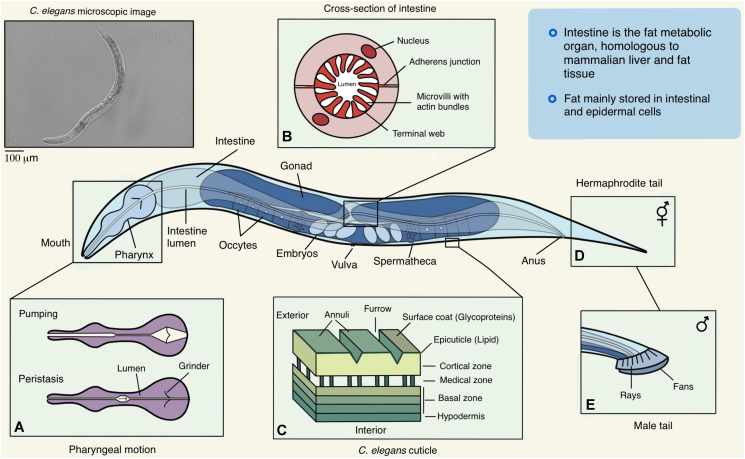
\includegraphics[width=\imsize]{gr1.jpg}
	\caption[ Anatomía del Caenorhabditis elegans adulto.]{ Anatomía del Caenorhabditis elegans adulto.La figura ilustra la anatomía fundamental del organismo modelo, Caenorhabditis elegans (C. elegans), que es crucial para contextualizar sus características biológicas. La anatomía básica de C. elegans comprende varios componentes esenciales. (A) La boca está formada por seis labios simétricos que crean una cavidad circular de \qtyrange{1}{2}{\micro\metre}, facilitando la ingestión de alimento que se dirige al órgano de alimentación, la faringe. (B) El intestino se compone de 20 células epiteliales grandes organizadas bilateralmente en pares simétricos para formar un tubo largo con un lumen central. (C) La cutícula, que en adultos jóvenes tiene un grosor de aproximadamente \qty{0.5}{\micro\metre}, consta de cuatro capas principales: epicutícula, cortical, medial y basal. (D y E) La cola de la hermafrodita se estrecha hacia un extremo afilado, mientras que la cola del macho se caracteriza por ser roma y contiene un aparato copulador distintivo.  (Adaptado de \protect\cite{yue_caenorhabditis_2021} ).}\label{fig:sistema_anatomia}
\end{figure}



\subsection{Sistema nervioso}





En el campo de la neurobiología, la comprensión de cómo el sistema nervioso desempeña sus funciones integrativas e instructivas es de suma importancia. El sistema nervioso es una red compleja de neuronas interconectadas, y la transmisión de actividad entre estas neuronas es esencial para su funcionamiento. Las sinapsis químicas y eléctricas son los elementos clave a través de los cuales la actividad de una neurona se comunica con otras. Además, cada neurona normalmente recibe entradas de múltiples neuronas presinápticas, y las interacciones entre estas entradas son cruciales para determinar la respuesta de la neurona postsináptica. Por consiguiente, la estructura de la red y las propiedades de las sinapsis son los principales determinantes del flujo de información en el sistema nervioso \cite{toyoshima_deducing_2022}.

En el caso específico de C. elegans, encontramos dos sistemas nerviosos prácticamente independientes. El sistema nervioso somático, presente en el hermafrodita adulto, consta de 302 neuronas agrupadas en 118 clases distintas, mientras que el sistema nervioso faríngeo, que se encarga de la alimentación, comprende 20 neuronas distribuidas en 14 clases. Estos dos sistemas nerviosos están conectados por una única conexión sináptica eléctrica entre las neuronas RIP somáticas y las neuronas I1 faríngeas \cite{fang-yen_illuminating_2015}. Por otro lado, los machos de C. elegans poseen 381 neuronas y 92 células gliales y de soporte. Aproximadamente la mitad de las neuronas se ubican en la cabeza, rodeando un neuropilo central denominado anillo nervioso, mientras que el resto se distribuye a lo largo del cordón ventral y en los ganglios de la cola. Las neuronas específicas de los machos se encuentran principalmente en la cola copulatoria. En ambos sexos, cada neurona se identifica de manera única en diferentes individuos por su posición y morfología característica.

Las neuronas de C. elegans se designan mediante un código de 2 o 3 letras, acompañado en ocasiones de un número, seguido generalmente de letras L (izquierda), R (derecha), D (dorsal) o V (ventral) para especificar su posición anatómica. Estas neuronas se pueden clasificar como sensoriales, interneuronas y motoras, en función de sus características anatómicas y su conectividad sináptica (\Cref{fig:conectoma_a, fig:sistema_nervioso2}). Las neuronas sensoriales poseen terminaciones sensoriales, ya sea que se haya demostrado su funcionalidad o no. Las neuronas motoras establecen sinapsis con células musculares, mientras que las interneuronas forman numerosas conexiones con otras neuronas. No obstante, estas categorías son en cierta medida arbitrarias, ya que muchas neuronas abarcan dos o más funciones. Por ejemplo, las neuronas motoras excitadoras de tipo B establecen sinapsis con diversas neuronas y, además, se ha demostrado que desempeñan una función sensorial propioceptiva. Para obtener una lista completa de las neuronas de C. elegans, su linaje y descripciones detalladas, se puede consultar la base de datos WormAtlas (\url{https://www.wormatlas.org/}).


 \begin{figure}[h!]
	\centering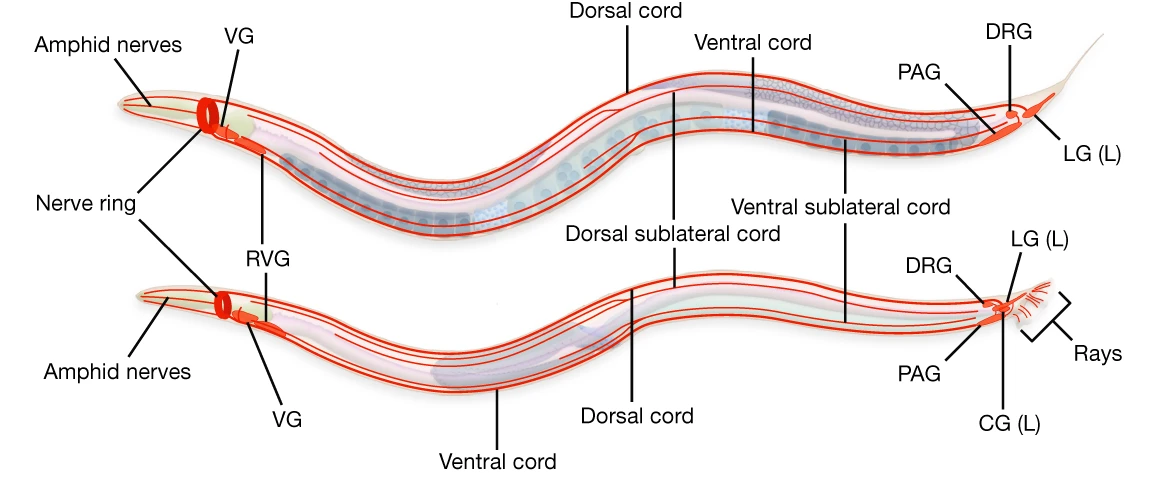
\includegraphics[width=\imsizeL]{conectoma_a.png}
	\caption[Representación del Sistema Nervioso de Caenorhabditis elegans.]{ Representación del Sistema Nervioso de Caenorhabditis elegans. En el hermafrodita adulto y el macho adulto, se destacan los principales ganglios y tractos nerviosos, dispuestos desde el extremo anterior hacia el izquierdo. De particular relevancia son los centros neurales de conectividad, entre los que se incluyen el anillo nervioso y, exclusivamente en el macho, el ganglio preanal. Se han identificado y etiquetado áreas significativas, tales como el ganglio cloacal (CG), el ganglio dorsorrectal (DRG), el ganglio lumbar (LG), el ganglio preanal (PAG), el ganglio retrovesicular (RVG) y el ganglio ventral (VG).   (Figura adaptada de \protect\cite{cook_whole-animal_2019}).}\label{fig:conectoma_a}
\end{figure}


 \begin{figure}[h!]
	\centering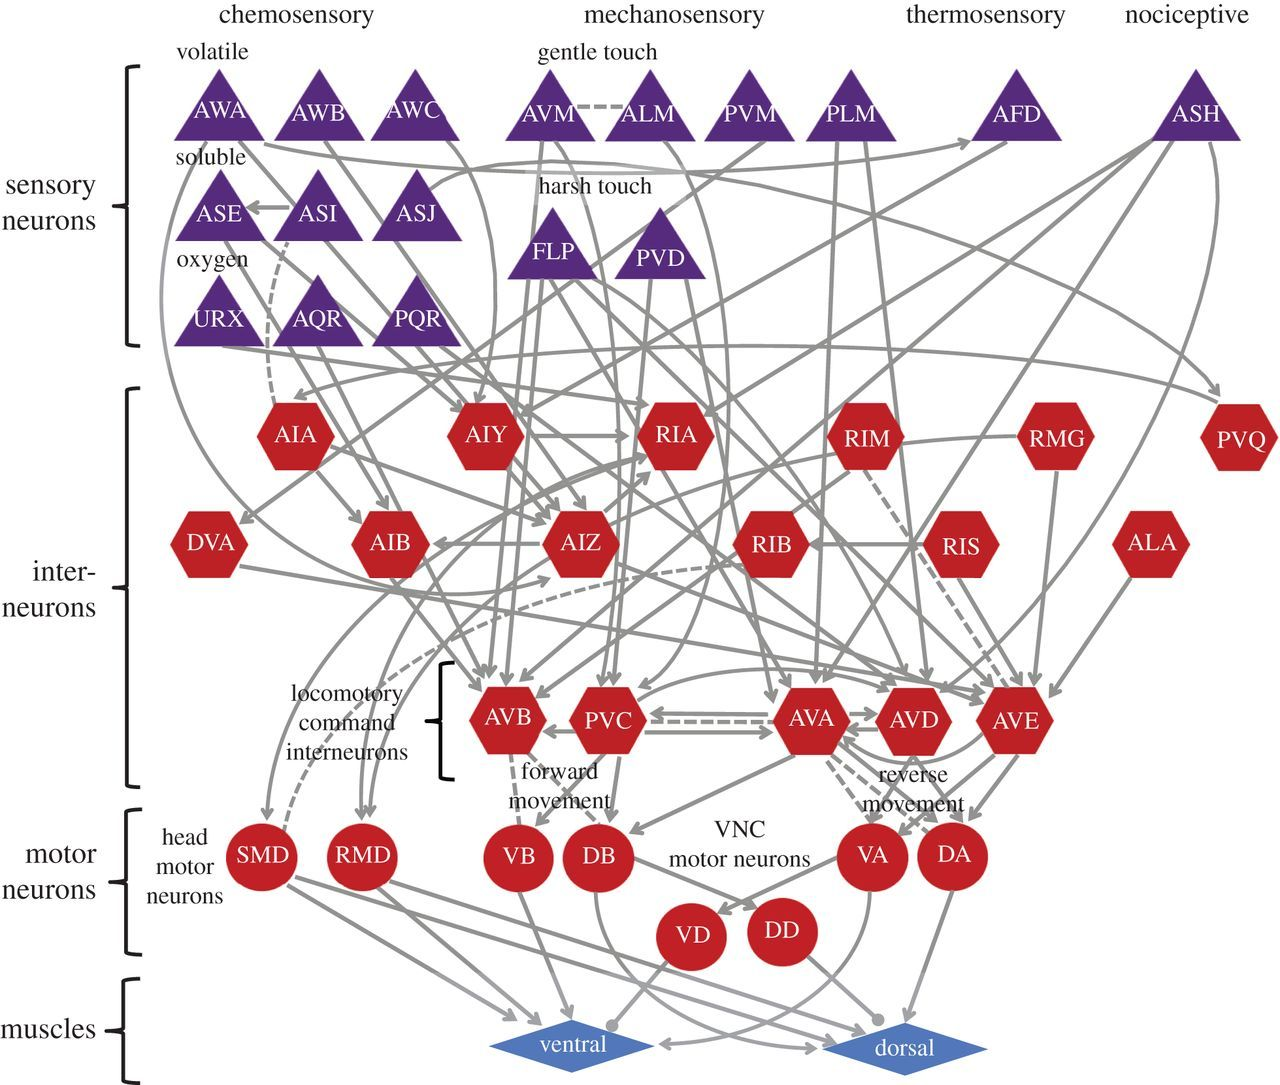
\includegraphics[width=\imsize]{rstb20140212f02.jpg}
	\caption[ Diagrama del circuito parcial del sistema nervioso somático y la musculatura de C. elegans. ]{ Diagrama del circuito parcial del sistema nervioso somático y la musculatura de C. elegans.  En el diagrama, se representan las neuronas sensoriales mediante triángulos, las interneuronas mediante hexágonos, las neuronas motoras mediante círculos y los músculos mediante diamantes. Las flechas indican conexiones sinápticas, que pueden ser de naturaleza excitatoria o inhibitoria, mientras que las líneas discontinuas señalan conexiones mediante sinapsis eléctricas. El cordón nervioso ventral (VNC) se identifica como una parte fundamental del sistema.  (Adaptado de \protect\cite{shibue_deconvolution_2020}).}\label{fig:sistema_nervioso2}
\end{figure}


\subsection{Locomoción}

La investigación en el comportamiento de Caenorhabditis elegans (C. elegans) se ha enfocado principalmente en el procesamiento sensorial de los estímulos ambientales que influyen en el patrón de locomoción de estos nematodos. La locomoción en C. elegans se lleva a cabo mediante un mecanismo de propulsión ondulatoria, caracterizado por la generación de un tren de ondas que se propaga a lo largo del cuerpo del gusano. La orientación del gusano, ya sea en su lado izquierdo o derecho, determina la formación de estas ondas, que resultan de la secuencia de contracciones y relajaciones alternas de los músculos longitudinales en la pared corporal, tanto dorsal como ventral. Tres fuerzas fundamentales permiten el movimiento en superficies sólidas: el esqueleto hidrostático, que sirve como punto de apoyo para la acción muscular; la tensión superficial, que presiona al gusano contra su sustrato; y la fricción entre el gusano y su superficie de apoyo, que permite que las ondas corporales avancen sin deslizamiento, generando así la propulsión hacia adelante.

El sistema muscular responsable de la locomoción en C. elegans comprende 95 células musculares de la pared corporal que reciben entradas excitatorias a través de uniones neuromusculares colinérgicas (NMJ) y entradas inhibitorias a través de NMJ GABAérgicas \cite{bono_neuronal_2005}. Diferentes clases de neuronas motoras distribuidas a lo largo del cuerpo regulan diferentes regiones de la musculatura. Un conjunto de neuronas dorsales (DB, DD) y ventrales (VB, VD), tanto excitatorias como inhibitorias, controla el movimiento hacia adelante, mientras que otro conjunto de neuronas (DA, DD y VA, VD) gobierna el movimiento hacia atrás. La interconexión de estas neuronas implica que, por ejemplo, la excitación de las neuronas motoras colinérgicas ventrales, como VB o VA, en una región específica de la musculatura ventral, resulta en la relajación de la musculatura dorsal opuesta debido a la inhibición de las neuronas motoras GABAérgicas (DD). Esto lleva a una curvatura específica del cuerpo. Esta inhibición recíproca es de suma importancia, especialmente en los movimientos de escape rápidos (\Cref{fig:movimiento}).



 \begin{figure}[h!]
	\centering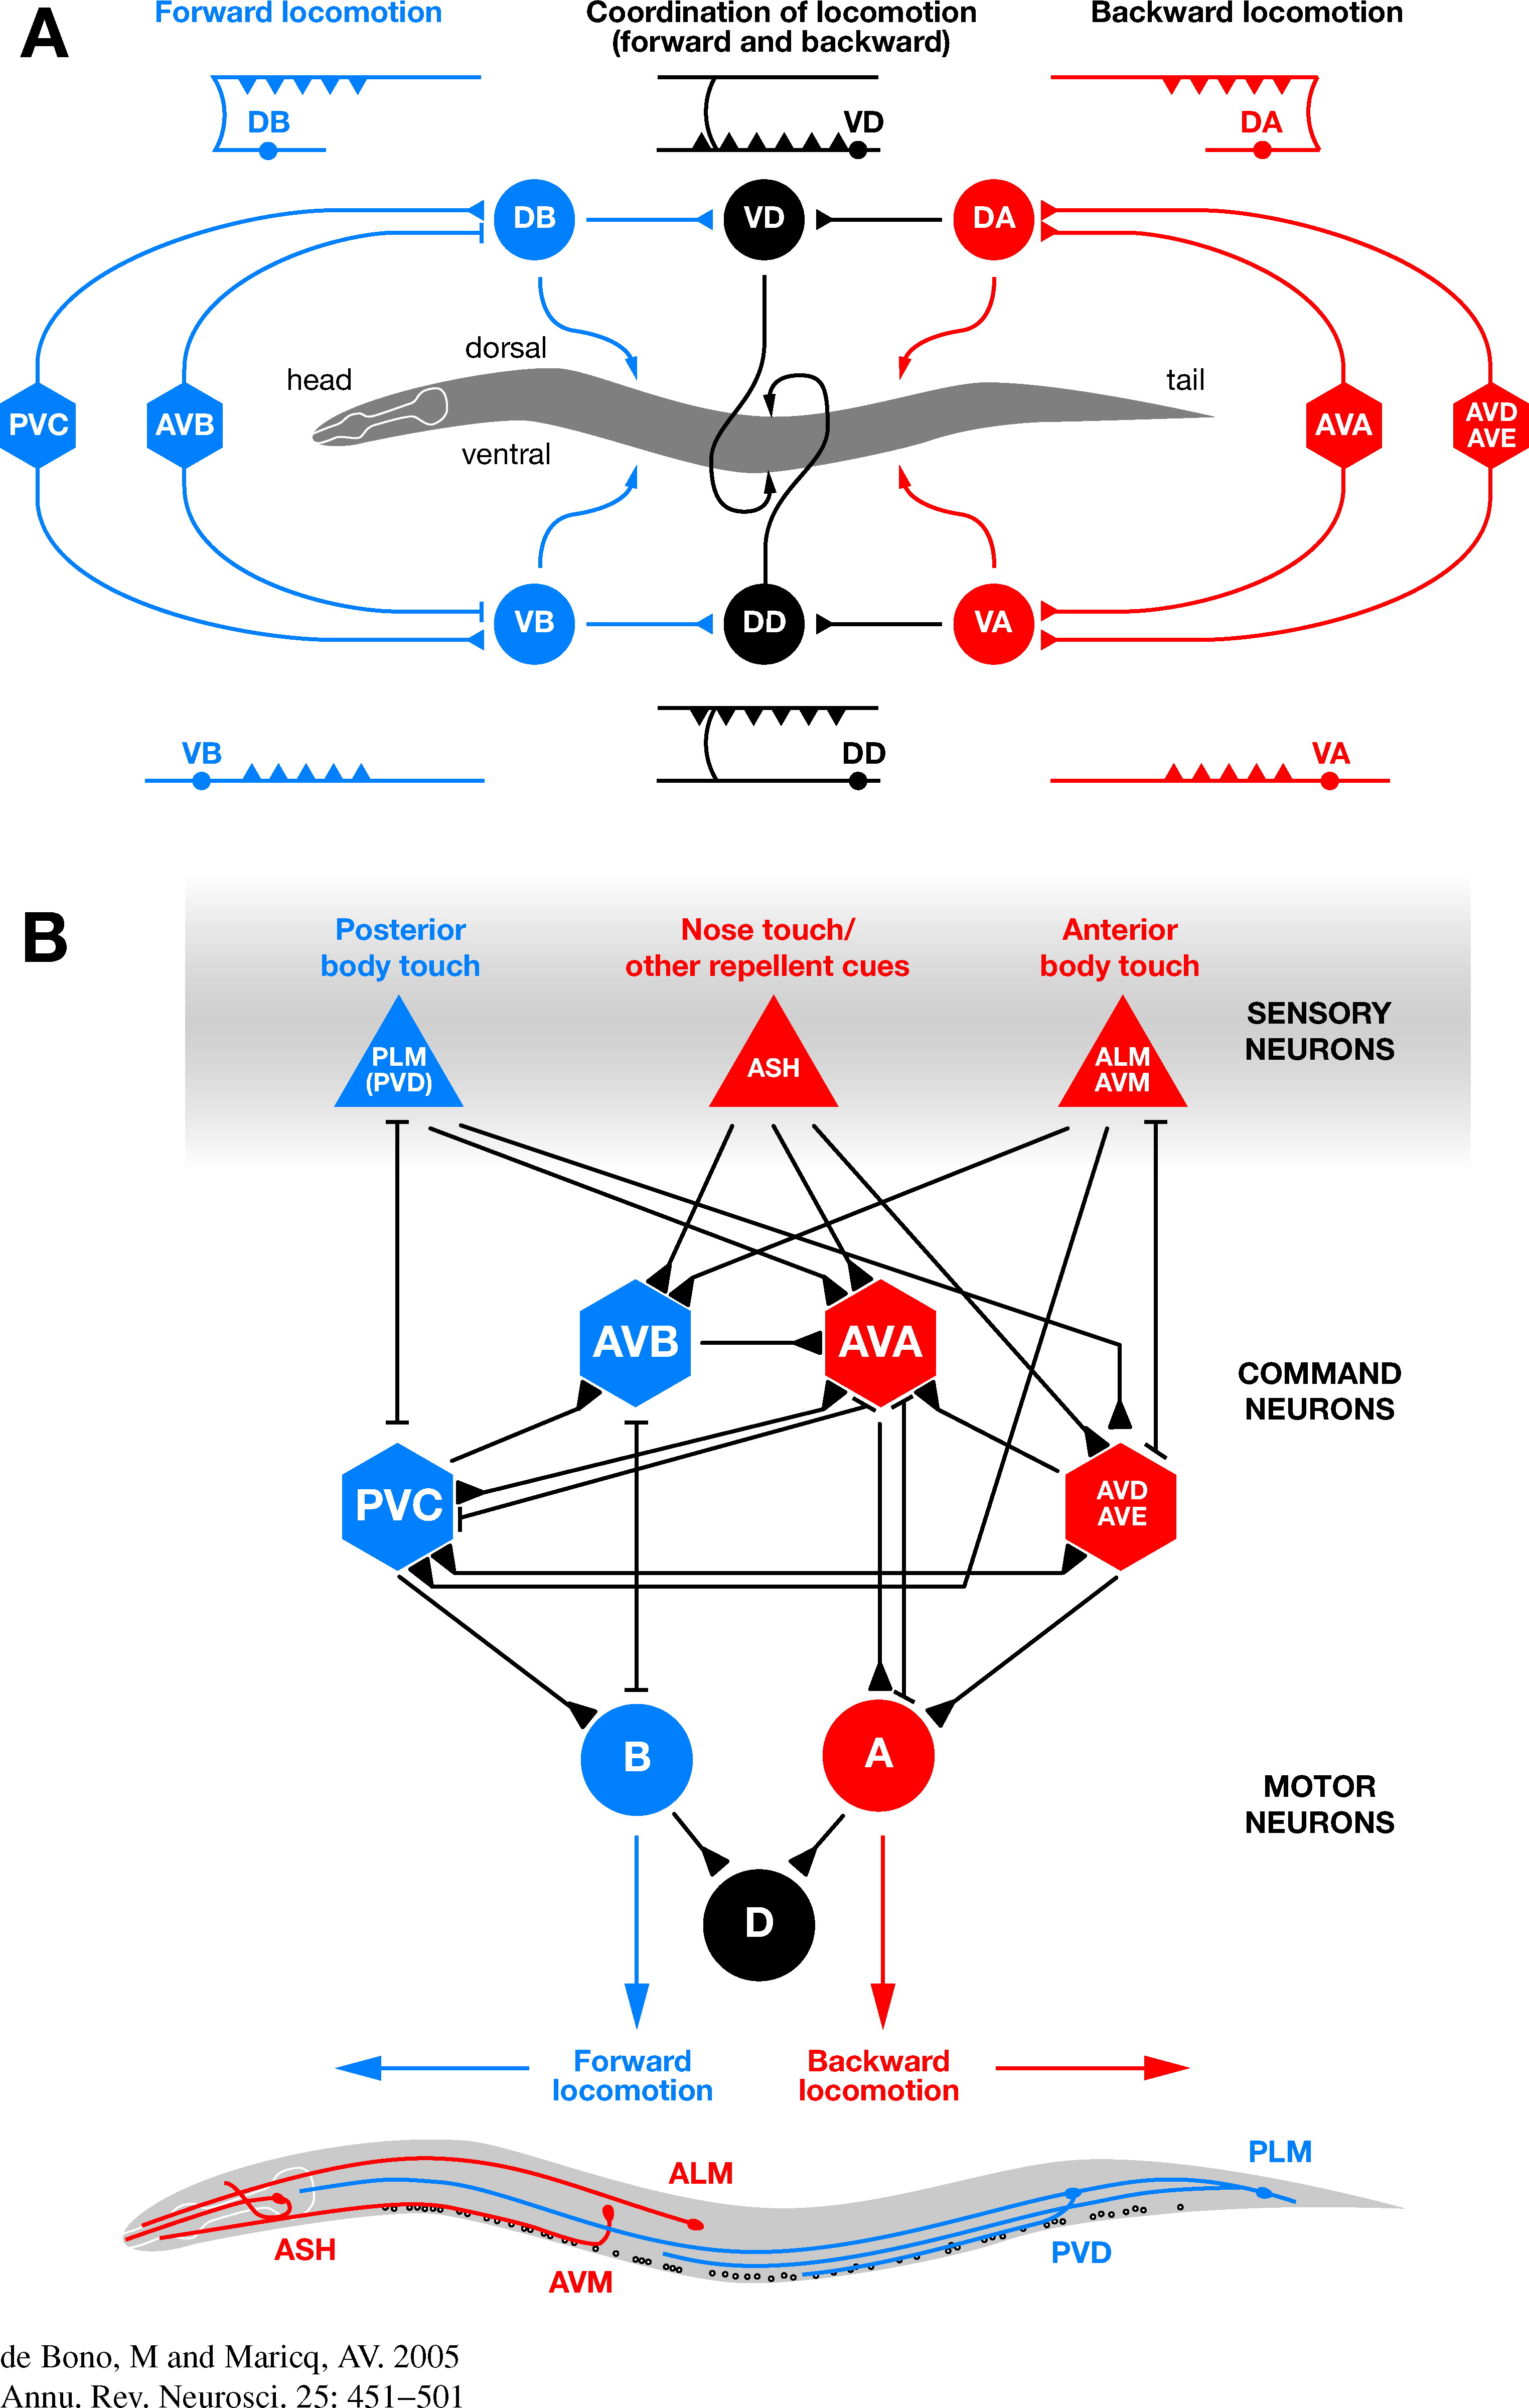
\includegraphics[width=\imsize]{ne280451.f1.jpeg}
	\caption[ Control Neuronal de la Locomoción hacia Adelante y Hacia Atrás ]{ Control Neuronal de la Locomoción hacia Adelante y Hacia Atrás. A) En este diagrama, se detalla la compleja conectividad entre las interneuronas de comando (hexágonos) y las neuronas motoras (círculos). Las sinapsis químicas se indican mediante triángulos, mientras que las eléctricas se representan mediante barras. Los pequeños círculos reflejan los cuerpos celulares, y las líneas representan los procesos neuronales, destacando las sinapsis de las neuronas motoras. Todos los cuerpos celulares se ubican en el lado ventral del gusano. 	B) El circuito que regula la respuesta al tacto, fundamental en la generación de movimientos de avance y retroceso, se ilustra en el diagrama superior. Se resalta la conectividad entre las neuronas sensoriales (triángulos), las interneuronas de comando y las neuronas motoras. Las neuronas PVD desempeñan un papel esencial en la respuesta a estímulos táctiles intensos, mientras que las neuronas PLM, ALM y AVM son críticas para las respuestas a estímulos táctiles más suaves. En el diagrama inferior, se presenta la morfología de las neuronas sensoriales en un hermafrodita adulto (con la parte anterior hacia la izquierda y la parte ventral hacia abajo). Las áreas coloreadas en azul y rojo representan las neuronas que están predominantemente involucradas en la locomoción hacia adelante y hacia atrás, respectivamente.   (Adaptado de \protect\cite{bono_neuronal_2005}).}\label{fig:movimiento}
\end{figure}



\subsubsection{Movimiento hacia adelante o hacia atrás}


La capacidad de moverse hacia adelante y hacia atrás en C. elegans está coordinada por neuronas sensoriales especializadas que detectan el tacto en regiones anteriores (AVM, ALM) o posteriores (PVM, PLM) del cuerpo del gusano (consultar \Cref{fig:movimiento}B). Estas neuronas establecen conexiones eléctricas y sinápticas con un conjunto prominente de interneuronas. Aunque la naturaleza precisa de estas sinapsis químicas no ha sido completamente elucidada, se ha observado que las neuronas PLM y ALM establecen conexiones de unión gap con PVC y AVD, respectivamente. AVD, en conjunto con otra interneurona denominada AVA, inerva las neuronas motoras VA y DA, las cuales coordinan el movimiento hacia atrás. Por otro lado, PVC y las interneuronas AVB inervan las neuronas motoras VB y DB, regulando así el movimiento hacia adelante (consultar \Cref{fig:movimiento}A). A pesar de que las funciones de estas cuatro interneuronas parecen estar interconectadas y distribuidas (a través de conexiones sinápticas recíprocas o mediante neuronas adicionales), se presume que estas interneuronas son las mediadoras de las respuestas de retirada al tacto corporal y regulan la elección entre el movimiento hacia adelante y hacia atrás. Dada su relevancia en los movimientos de propulsión y retroceso, AVA, AVB, AVD y PVC son comúnmente denominadas interneuronas de comando.


\subsubsection{Nocicepción por la neurona polimodal ASH}\label{sec:toquenariz}

Es relevante señalar que C. elegans exhibe un mecanismo de nocicepción, respondiendo a una variedad de estímulos nocivos, como alta osmolaridad, contacto en la nariz, ciertos olores, metales pesados como \ce{Cu^{2+}} y \ce{Cd^{2+}}, pH bajo, alcaloides como la quinina y detergentes, con una respuesta de escape caracterizada por un rápido retroceso seguido de la reanudación del movimiento, generalmente en una dirección diferente. La identificación de las neuronas sensoriales mediadoras de estas respuestas de evitación se ha logrado mediante técnicas de ablación láser (consultar \Cref{table:sensorialceelegans}).   Sorprendentemente, a pesar de la diversidad en la naturaleza física y química de estos estímulos nocivos, todos ellos convergen en una única neurona, la neurona polimodal ASH. 

\begin{table}[h!]
	\centering
	\caption[Neuronas Sensoriales Mediadoras de las Respuestas Aversivas en C. elegans a Estímulos Nocivos.]{ Neuronas Sensoriales Mediadoras de las Respuestas Aversivas en C. elegans a Estímulos Nocivos.}
	\begin{tblr}{colspec={ll},
			row{odd} = {bg=gray8},
			row{even} = {bg=gray9},
			row{1} = {bg=red3, fg=white, font=\sffamily},
		}
		
		Estímulo Nocivo	 & Neurona sensorial\\
		Alta Osmolaridad  &  ASH \\
		Tacto en la Nariz & ASH, OLQ, FLP \\
		Olores & ASH, ADL, AWB\\
		Metales Pesados & ASH, ADL, ASE\\
		Protones &   ASH, ADF, ASE, ASK \\
		Alcaloides & ASH, ASK \\
		Detergentes & ASH, ASK, PHA, PHB \\
	\end{tblr}
	\label{table:sensorialceelegans}
\end{table}


La neurona ASH es una neurona sensorial bilateral única que reside en la cabeza del gusano. Posee una dendrita bifurcada que se extiende hacia adelante a lo largo del lado ventral del gusano y termina en el extremo anterior del cuerpo. Además, presenta un axón que se extiende hacia atrás hasta el extremo posterior del gusano. La neurona ASH recibe información sensorial de diversos receptores químicos y mecanosensoriales a lo largo de su dendrita y axón. Cuando la neurona ASH se activa en respuesta a un estímulo nocivo, transmite señales a otras neuronas en el circuito de nocicepción, las cuales, a su vez, estimulan las neuronas motoras responsables del movimiento de retroceso en el gusano. De esta forma, el gusano ejecuta un rápido retroceso. Además de su papel en la locomoción de escape, la neurona ASH también interacciona con las neuronas responsables de los procesos de aprendizaje y memoria, permitiendo al gusano recordar y evitar estímulos nocivos en el futuro.



\subsection{Quimiosensación en C. elegans}\label{sec:quimiosensacion}

La quimiosensación desempeña un papel esencial en la vida de Caenorhabditis elegans (C. elegans), ya que le permite buscar alimento, evitar condiciones adversas, completar su desarrollo de manera adecuada y llevar a cabo el proceso de apareamiento. Este organismo detecta sustancias químicas a través de neuronas quimiosensoriales especializadas que extienden sus cilios sensoriales hacia el entorno. Estas neuronas quimiosensoriales se localizan en órganos específicos, incluyendo los anfídeos, fásmidos y labios internos, y su exposición al medio ambiente se facilita mediante aberturas reguladas por células gliales denominadas células de encaje y vaina. Además, en el caso de las neuronas amfídeas, un par adicional, conocido como AFD, desempeña un papel como termosensor. Un rasgo distintivo es que estas neuronas quimiosensoriales suelen presentarse en pares simétricos bilaterales, y los miembros de cada par, izquierdo y derecho, suelen compartir similitudes estructurales (Ver \Cref{table:quimico}). Tanto los estudios anatómicos como los funcionales han sugerido que las neuronas amfídeas y fásmidas participan activamente en los procesos de quimiosensación \cite{bargmann_chemosensation_2006}.

\begin{table}[h!]
	\centering
	\caption[Funciones y Propiedades de las Neuronas Quimiosensoriales.]{ Funciones y Propiedades de las Neuronas Quimiosensoriales. Estas neuronas desempeñan un papel crucial en diversos aspectos del comportamiento y la supervivencia de este organismo. }
	\begin{tblr}{colspec={X[l,1]X[l,4]},
			row{odd} = {bg=gray8},
			row{even} = {bg=gray9},
			row{1} = {bg=red3, fg=white, font=\sffamily},
		}
		
	Neurona & NeuronaFunción\\
	 ASE & Quimiotaxis soluble en agua \\
	 AWC & Quimiotaxis volátil, esperanza de vida, navegación \\
	 AWA & Quimiotaxis volátil, esperanza de vida (menor) \\
	 AWB & Evasión volátil \\
	 ASH & Nocicepción: Evasión osmótica, evasión del tacto nasal, evasión química, alimentación social \\
	 ASI & Formación de dauer, quimiotaxis (menor), navegación \\
	 ADF & Formación de dauer, quimiotaxis (menor) \\
	 ASG & Formación de dauer (menor), esperanza de vida, quimiotaxis (menor) \\
	 ASJ & Formación y recuperación de dauer, quimiotaxis (menor), esperanza de vida \\
	 ASK & Evasión (menor), quimiotaxis (menor), esperanza de vida, navegación \\
	 ADL & Evasión (menor), alimentación social	 
	\end{tblr}
	\label{table:quimico}
\end{table}

\subsubsection{Neuronas gustativas ASE}

En C. elegans, la capacidad de migrar hacia compuestos atractivos, como el cloruro (\ce{Cl^{-}}), en presencia de niveles elevados y uniformes de otros compuestos atractivos, como el sodio (\ce{Na^{+}}), destaca la especificidad de los sitios de unión de los diferentes atrayentes. Las neuronas gustativas ASE son las responsables de la detección de sales y sustancias atractivas solubles en agua. La quimiotaxis de C. elegans hacia cationes, aniones, nucleótidos cíclicos y aminoácidos fue inicialmente descrita por Ward \cite{ward_chemotaxis_1973}. Aunque la lista de compuestos atractivos ha aumentado con el tiempo, el número de sustancias solubles en agua conocidas como atrayentes sigue siendo limitado. 

La importancia de las neuronas sensoriales en las respuestas quimiosensoriales ha sido establecida mediante la ablación selectiva de neuronas específicas utilizando un microhaz láser, seguida de la evaluación de los comportamientos de los organismos tratados. La eliminación de un par de neuronas sensoriales amfídicas, conocidas como neuronas ASE, resulta en una disminución significativa en la capacidad de quimiotaxis hacia atrayentes solubles en agua, como \ce{Na^{+}},\ce{Cl^{-}}, AMPc, biotina, lisina y serotonina.  Es relevante destacar que la ablación simultánea de todas las neuronas amfídeas y fásmidas, excepto las ASE, no afecta la quimiotaxis, lo que sugiere un papel único de las neuronas ASE en la detección de sustancias solubles en agua. Posterior a la ablación de las neuronas ASE, se observa una respuesta quimiotáctica residual, aunque débil, hacia los atrayentes solubles en agua, la cual parece estar distribuida en diversas clases de neuronas, incluyendo ADF, ASG, ASI, ASK y ASJ. Es importante destacar que las dos neuronas ASE, ASER (derecha) y ASEL (izquierda), exhiben diferencias funcionales, ya que ASER tiene una preferencia por la detección de iones cloruro y potasio, mientras que ASEL muestra una preferencia por la detección de iones sodio.





\section{Conectoma}\label{sec:conectoma}



En esta sección, se analizan las técnicas y los resultados más significativos en el mapeo de las conexiones neuronales en organismos vivos, con un enfoque especial en Caenorhabditis elegans. Este organismo ha proporcionado el conectoma más completo registrado hasta la fecha y desempeñará un papel fundamental en la segunda parte de esta tesis, relacionada con los modelos de criticidad neuronal.

El sistema nervioso, aparentemente uniforme y cohesivo, encierra una complejidad celular casi inimaginable: miles de millones de neuronas que interactúan a través de trillones de sinapsis, formando circuitos para la percepción de estímulos, el almacenamiento de recuerdos y la generación de emociones. Esto plantea una cuestión fundamental: ¿qué ocurriría si pudiéramos trazar un mapa completo de estas conexiones? ¿Nos ayudaría a comprender el funcionamiento del cerebro? Este es el propósito de la \textquote{conectómica}, que consiste en la identificación sistemática de todas las conexiones en un sistema nervioso. Aunque el término es relativamente reciente, sus conceptos se remontan a décadas atrás, con los esfuerzos pioneros de Sydney Brenner en la década de 1960. Brenner eligió a Caenorhabditis elegans, apodado cariñosamente como el \textquote{gusano}, para llevar a cabo la ambiciosa tarea de mapear completamente su sistema nervioso \cite{portman_neural_2019}. A pesar de su tamaño diminuto, el sistema nervioso del gusano, compuesto por unas pocas centenas de neuronas, subyace a comportamientos complejos y flexibles. La tarea implicó la sección minuciosa del gusano en rebanadas delgadas, lo que permitió el estudio detallado de cada neurona y sus conexiones mediante microscopía (consulte la \Cref{fig:conectoma}). Este esfuerzo titánico se llevó a cabo en las décadas de 1970 y 1980, y se complementó con grabaciones de la actividad neuronal individual y la tinción de células para visualizar sus estructuras y patrones de proyección a través de microscopía óptica. En algunos casos, se utilizó la microscopía electrónica para examinar las sinapsis anatómicas presentes en estos circuitos microscópicos. El resultado fue el primer conectoma de su tipo, que se documentó en un influyente artículo de 1986, comúnmente denominado \textquote{La Mente del Gusano} \cite{white_structure_1997}. A lo largo del tiempo, este conectoma ha sido objeto de refinamientos significativos, y neurobiólogos de todo el mundo han trabajado incansablemente para comprender cómo emergen los comportamientos a partir de los circuitos descritos.


Hoy en día, disponemos de una abundante evidencia que respalda la idea de que tanto los conectomas de uniones gap como los conectomas sinápticos en C. elegans poseen propiedades de red complejas. El conectoma de C. elegans exhibe una organización jerárquica, en la que las neuronas sensoriales predominan en las conexiones pre-sinápticas, mientras que las neuronas motoras se destacan en las conexiones post-sinápticas. Además, se aprecia una estructura de comunidad modular entre neuronas que comparten funciones relacionadas. La conectividad sináptica binaria del gusano se ajusta a un patrón de organización de mundo pequeño y muestra una distribución de grados con colas largas. Además, se ha identificado una ocurrencia mayor que la esperada al azar de ciertos motivos de tripletes y cuartetos en la red. Un hallazgo intrigante es que las neuronas centrales del conectoma de C. elegans se organizan en una red altamente interconectada, a menudo denominada el \textquote{club rico}. Este núcleo de la red está principalmente compuesto por interneuronas que comandan los circuitos locomotores, exhiben una alta centralidad (es decir, muchos de los caminos más cortos entre las neuronas periféricas atraviesan una o más de estas interneuronas centrales del club rico) y facilitan numerosas conexiones de largo alcance entre módulos funcionales distantes. Este club rico emerge temprano en el desarrollo del conectoma \cite{schroter_micro-connectomics_2017}.  En promedio, se ha observado que el número mínimo de sinapsis químicas que conectan las neuronas sensoriales y las neuronas motoras es de aproximadamente 3. Esto implica que, en promedio, la ruta más corta desde una neurona sensorial hacia una neurona motora requiere el paso por dos interneuronas. En la categoría de interneuronas, un reducido grupo de interneuronas centrales, denominadas neuronas de comando, poseen la mayoría de las sinapsis en la red. Forman una red altamente interconectada propia que controla los movimientos hacia adelante y hacia atrás. Estas neuronas actúan como neuronas pre-sinápticas con respecto a las neuronas motoras del cuerpo y como neuronas post-sinápticas con respecto a una amplia variedad de otras interneuronas, que a su vez se conectan con las neuronas sensoriales \cite{flavell_dynamic_2022}. 


Diversos conectomas adicionales se han creado en diferentes organismos, ya sea a nivel sináptico, como en la larva de renacuajo del ascidia Ciona intestinalis \cite{ryan_cns_2016} y el anélido marino Platynereis dumerilii \cite{veraszto_whole-animal_2020}, o en sistemas nerviosos centrales completos, como el sistema nervioso central larvario de la mosca de la fruta Drosophila melanogaster \cite{scheffer_connectome_2020} y la larva de tres días del anélido Platynereis dumerilii. Finalmente en el 2023  Winding et al.  \cite{winding_connectome_2023}  obtuvieron el primer conectoma de cerebro completo de un cerebro de insecto, la larva de la mosca del vinagre ( Drosophila melanogaster ). Este  trabajo,  inspirará nuevos estudios sobre circuitos neuronales y arquitecturas de aprendizaje automático.

 

 
 
 
 

\begin{figure}[h!]
	\centering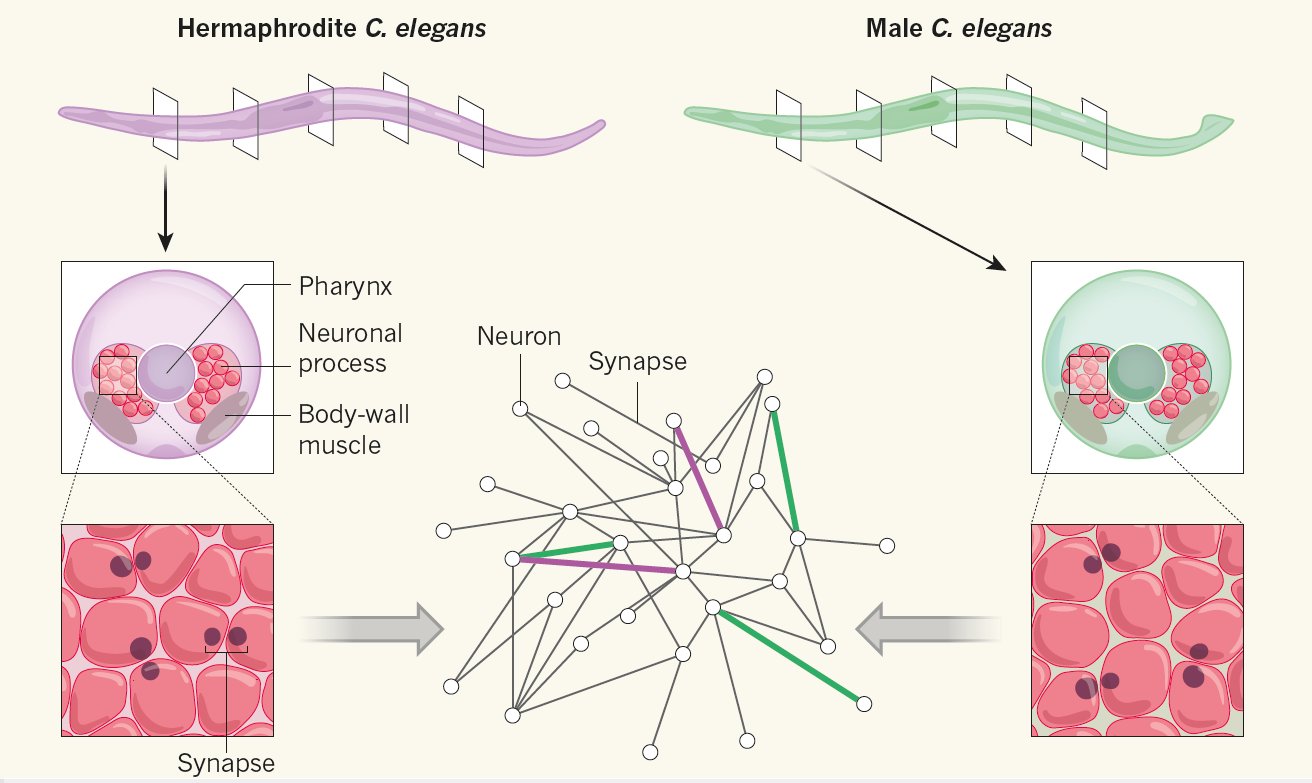
\includegraphics[width=\imsize]{conectoma.png}
	\caption[Mapeo del conectoma  del gusano.  ]{ Mapeo del conectoma  del gusano.  Cook et al. \protect\cite{cook_whole-animal_2019}  llevaron a cabo el mapeo de los sistemas nerviosos completos del gusano nematodo Caenorhabditis elegans, tanto del sexo hermafrodita como del macho, con una asombrosa resolución subcelular.   En la parte superior de la figura, se aprecia el uso de decenas de miles de secciones seriadas que abarcan la mayor parte del cuerpo del gusano adulto. Se obtuvieron imágenes de microscopía en baja y alta resolución de estas secciones, lo que permitió revelar la anatomía de una sección típica, incluyendo los procesos neuronales y las conexiones sinápticas. Estas imágenes sirvieron de base para la construcción de un conectoma, un mapa que visualiza las conexiones entre todas las neuronas. En el centro de la figura, se muestra una versión simplificada de este conectoma. La mayoría de las conexiones se encuentran en ambos sexos (indicadas en gris), aunque algunas son exclusivas de un sexo o presentan una mayor fortaleza en uno que en el otro (resaltadas en púrpura y verde).   (Adaptada de \protect\cite{portman_neural_2019}).}\label{fig:conectoma}
\end{figure}


\subsection{Métodos de Reconstrucción de Conectomas}

La reconstrucción de conectomas se ha beneficiado de diversas metodologías. La microscopía electrónica ha permitido la reconstrucción a nivel sináptico, mientras que la combinación de técnicas de inyección de trazadores con imágenes ópticas de tomografía seriada de alto rendimiento ha posibilitado la reconstrucción de alta resolución en ratones. Además, la recopilación sistemática de datos de una gran cantidad de experimentos de trazado ha dado como resultado matrices de consenso que condensan las conexiones cerebrales en gatos, monos y ratas. Los avances en técnicas de resonancia magnética de difusión in vivo están haciendo que sea cada vez más factible reconstruir conectomas a macroescala en cerebros individuales de grandes simios y humanos. Con el desarrollo de técnicas como CLARITY y la Imagen de Luz Polarizada en 3D (3D-PLI), es probable que se obtengan reconstrucciones sin precedentes de la conectividad del conectoma en animales y humanos en el futuro \cite{heuvel_comparative_2016}.


\subsection{Conectoma de C. elegans Completo (Cook et al., 2019)}

Hasta el año 2019, el conectoma más completo se basaba en la reconstrucción realizada por White et al. \cite{white_structure_1997}. No obstante, es fundamental tener en cuenta que este conectoma se limitaba al sexo hermafrodita, lo que generaba incertidumbre acerca de posibles diferencias en el cableado entre sexos.  Además, la construcción manual del conectoma original planteaba inquietudes sobre la precisión de los datos. Para abordar estos desafíos, Cook et al. \cite{cook_whole-animal_2019} desarrollaron un software especializado que permitió la reconstrucción del conectoma del macho adulto de C. elegans, una región que alberga circuitos exclusivos de este sexo. Posteriormente, Cook et al. \cite{cook_whole-animal_2019} informaron sobre la reconstrucción del conectoma masculino en su totalidad, incluyendo el anillo nervioso, una región crucial para el procesamiento de información en el gusano. Además, los autores emprendieron la tarea de reconstruir completamente el conectoma hermafrodita desde cero, aprovechando su software para reanalizar las microfotografías originales de la década de 1980. 

La \Cref{fig:conectomaa} presenta el conectoma de ambos sexos. Estos nuevos conectomas aportan una riqueza de información que promete avanzar significativamente en la comprensión del campo. Mientras que los conectomas originales simplemente indicaban la presencia de sinapsis, Cook et al. [16] proporcionaron información más detallada, que incluye la ubicación física y el peso de cada sinapsis, un indicador indirecto de la fuerza de la conexión en función de su tamaño físico. Este nivel de detalle permitirá análisis y modelados más sofisticados de la función de los circuitos neuronales. A través de su software, los investigadores también identificaron miles de conexiones previamente pasadas por alto en el hermafrodita. 

Utilizando herramientas de teoría de redes, introdujeron nuevas clasificaciones de grupos de neuronas en función de sus conexiones. Al comparar sus reconstrucciones de los lados izquierdo y derecho del gusano, que son en gran medida simétricos, los autores determinaron una alta precisión en los datos del conectoma. Los nuevos conectomas además incorporan detalles inéditos sobre las salidas del sistema nervioso, incluyendo conexiones previamente desconocidas con el intestino, la epidermis y la gónada masculina, lo cual inspira nuevas perspectivas en la fisiología y el metabolismo del gusano. También se identificó una complejidad inesperada en el control de los músculos del cuerpo \cite{portman_neural_2019}. 

A pesar de estos avances, el estudio presenta ciertas limitaciones, como la incertidumbre respecto a la cantidad de variabilidad entre individuos, la falta de claridad en cuanto a cómo la fuerza de una conexión se relaciona con su tamaño físico y el desafío de inferir la función únicamente a partir de la estructura del conectoma. En resumen, los conectomas representan mapas de posibilidades y, aunque revelan la totalidad de las sinapsis, proporcionan escasas pistas sobre cuáles están activas en un momento dado. 


 \begin{figure}[h!]
	\centering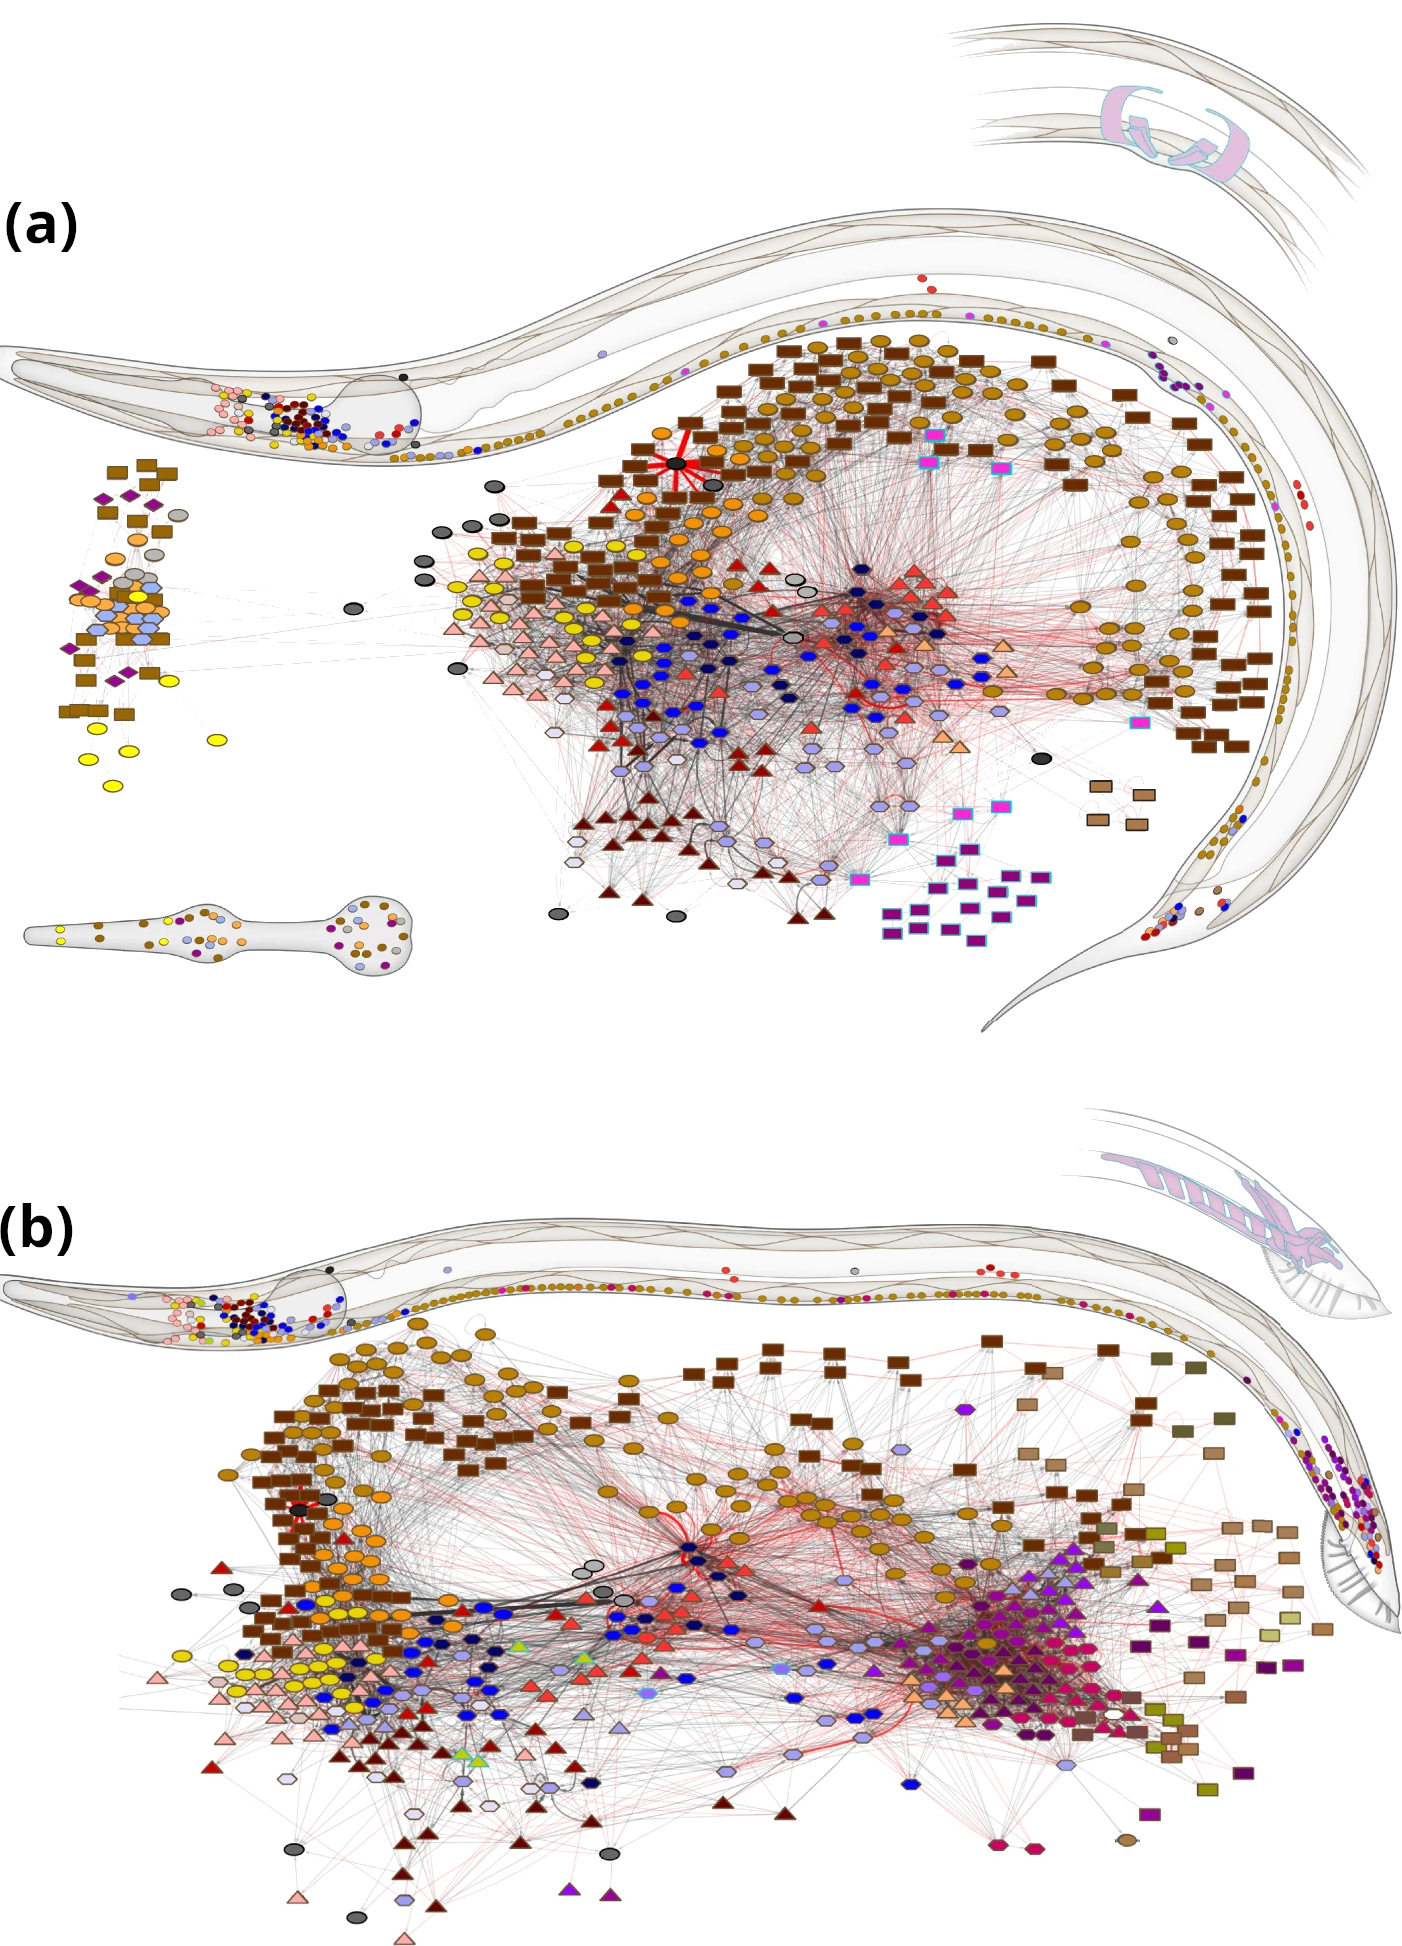
\includegraphics[width=\imsize]{conectoma_b.png}
	\caption[Conectividad del Sistema Nervioso  de C. elegans. Adultos.]{ Conectividad del Sistema Nervioso  de C. elegans. Adultos. (a) Representación del hermafrodita adulto. (b) Representación del macho adulto. En los cuadros ubicados en la esquina superior derecha de cada imagen, se resalta la ubicación de los músculos sexuales. Los diagramas de los gusanos indican la posición de los núcleos celulares.  En los grafos, la disposición de los vértices se basa en un algoritmo que agrupa las células altamente conectadas. Los bordes dirigidos, representados por flechas negras, indican las sinapsis químicas, mientras que los bordes no dirigidos, marcados con líneas rojas, representan las conexiones gap junctional. El ancho y la transparencia de las líneas denotan la fuerza de las conexiones. Una clave única se emplea para interpretar los diagramas de la red: triángulos para las neuronas sensoriales, hexágonos para las interneuronas, óvalos o círculos para las neuronas motoras, y rectángulos para los músculos. Los colores cumplen distintas funciones: varios tonos de rojo identifican las categorías de neuronas sensoriales según la modalidad y similitud de conectividad; tonos de azul señalan las categorías de interneuronas de acuerdo con su asignación a una capa específica; las clases de neuronas motoras se representan en varios tonos de amarillo y naranja, como se describe en el texto; por último, los órganos terminales no musculares se destacan en blanco, gris o negro.  (Adaptada de \protect\cite{cook_whole-animal_2019}).}\label{fig:conectomaa}
\end{figure}


\subsubsection{Matrices de adyacencia}


La matriz de adyacencia, que describe la estructura del sistema nervioso como un grafo de conectividad, se abstrae a partir de los mapas neuronales como una matriz de adyacencia con pesos que cuantifican la cantidad total de conectividad física entre cada par de células y se obtienen a partir de la suma de los tamaños de las conexiones sinápticas, que a menudo consisten en múltiples sinapsis. Dado que gran parte del sistema nervioso de C. elegans está compuesto por procesos simples y no ramificados que se encuentran en haces longitudinales donde establecen sinapsis de paso, se utilizó el método de anotación para estimar el tamaño de la mayoría de las sinapsis, contando las secciones atravesadas por la estructura sináptica. La cantidad de secciones varía entre 1 y 23 para las sinapsis químicas en el hermafrodita y entre 1 y 41 en el macho, mientras que para las sinapsis eléctricas oscila entre 1 y 20 en el hermafrodita y entre 1 y 30 en el macho. El grafo del conectoma hermafrodita consta de 460 nodos, que comprenden 302 neuronas, 132 músculos y 26 órganos terminales no musculares, mientras que el grafo del macho tiene 579 nodos, compuestos por 385 neuronas, 155 músculos y 39 órganos terminales no musculares. Estos grafos incluyen respectivamente 4.887 aristas químicas (con direccionalidad) y 1.447 aristas de unión en hendidura (sin direccionalidad) en el hermafrodita, y 5.315 químicas y 1.755 de unión en hendidura en el macho. A pesar de ser grafos dispersos, representan el 3,2 \% y el 2,4 \% de todas las aristas posibles en el caso del hermafrodita y el macho, respectivamente. Si se consideran todas las aristas sin direccionalidad en ambos sexos, se establece una conectividad débil, ya que existe al menos un camino que conecta cada par de nodos. La fracción de conectividad física debida a las uniones en hendidura varía ampliamente entre las clases de neuronas, fluctuando entre más del 90 \% y menos del 5 \% para las interneuronas no faríngeas. Los grafos de conectividad bidimensionales generados mediante métodos computacionales revelan las rutas de flujo de la información sensorial, con un pequeño número de pasos sinápticos (generalmente entre 1 y 5) entre las neuronas sensoriales y los órganos terminales, lo que sugiere una naturaleza de red "feedforward". La disposición de los nodos en los grafos muestra similitudes notables con la neuroanatomía del gusano, lo que refleja un cableado eficiente, una característica común en los sistemas nerviosos, incluso en C. elegans \cite{cook_whole-animal_2019}. .



La matriz de adyacencia generada se encuentra disponible en archivos de Excel que describen cada sinapsis, sus propiedades y un identificador único. Este número de identificación puede ingresarse en la página de neuronas de WormWiring (\url{http://wormwiring.org/}), lo que permite la ubicación de la sinapsis en el mapa. Al hacer clic en la sinapsis en el mapa, se acceden a las microfotografías pertinentes para su visualización.



\section{ Registro a Gran Escala de la Actividad Neuronal en C. elegans}


En los apartados  previos, se ha abordado la caracterización de las conexiones neuronales desde un enfoque principalmente estructural. Aunque el conectoma estructural proporciona una visión esencial del sistema nervioso, su comprensión integral se ve limitada por esta perspectiva.  Sin embargo, en la búsqueda de una comprensión más integral, la neurociencia ha desarrollado enfoques innovadores que tratan de cerrar la brecha entre la estructura anatómica y la función de los circuitos neuronales.

Estos nuevos enfoques aprovechan indicadores fluorescentes de actividad neuronal, permitiendo la observación en tiempo real del flujo de señales a través del sistema nervioso de C. elegans mientras el organismo se encuentra en un estado de comportamiento libre. Esta dinámica actividad neuronal se superpone con el conectoma estructural, proporcionando así una ventana a cómo la estructura física influye en la función.

Este apartado se centra en exponer los experimentos más recientes que siguen esta línea de investigación. La neurociencia de sistemas ha experimentado una tendencia general hacia la obtención de una imagen más completa de la actividad neuronal en el cerebro. La grabación simultánea de poblaciones neuronales ha emergido como una técnica superior en comparación con las grabaciones secuenciales de unidades individuales. No solo permite la captura de información de múltiples neuronas en un período de tiempo más corto, sino que también proporciona la oportunidad de realizar descubrimientos inesperados gracias a la simultaneidad de las grabaciones.


El registro de la actividad neuronal en todo el cerebro es atractivo debido a su potencial de ofrecer una visión exhaustiva. La idea subyacente es que el registro de la actividad de todas las neuronas de un organismo con un mapeo detallado de las conexiones neuronales podría eliminar las restricciones convencionales que dificultan la comprensión de fenómenos neuronales específicos. Esto reduciría la posibilidad de atribuir observaciones no explicadas a neuronas no registradas o conexiones no identificadas, lo que contribuye a la mejora de los modelos y al refinamiento de nuestra comprensión en este campo.


Aunque en organismos con sistemas nerviosos más complejos, como los vertebrados, esta perspectiva presenta desafíos sustanciales debido al aumento en la dimensionalidad de los datos, en organismos más pequeños, como C. elegans, se han logrado mediciones de actividad cerebral casi completa a nivel de una sola célula. Estos logros prometen brindar conceptos que pueden extrapolarse a redes de mayor tamaño.

Uno de los sujetos de estudio más exitosos en esta área es la larva del pez cebra. Investigadores han observado el cerebro de estos animales mientras llevan a cabo la natación ficticia y se mantienen inmovilizados en agar. Este avance se ha logrado mediante técnicas de microscopía de lámina de luz, lo que ha permitido la identificación de diversos patrones de actividad y sus relaciones en contextos de comportamiento. Además, otro organismo modelo que se presta bien a este tipo de análisis es el nematodo C. elegans. 

Este organismo destaca, en particular, por su transparencia óptica, siendo el primero en el que se expresó la proteína verde fluorescente (GFP). Este hito desencadenó una revolución en la imagenología biológica en tiempo real. Más recientemente, los investigadores han realizado trabajos pioneros para monitorear la actividad neuronal y muscular en gusanos a través de la fluorescencia de indicadores de calcio. Varios laboratorios han tenido éxito en la captura de imágenes de todo el cerebro de C. elegans \cite{kaplan_nested_2020,kato_global_2015,yemini_neuropal_2021}, demostrando que las actividades neuronales globales generan una diversidad de estados en los que se representan comportamientos característicos, como avanzar, retroceder y girar \cite{kato_global_2015}. Además, se han obtenido imágenes de todo el cerebro en animales en movimiento libre, lo que ha permitido la identificación de actividades relacionadas con comportamientos específicos \cite{kaplan_nested_2020}.


En este trabajo, nuestro enfoque se centrará principalmente en C. elegans. A pesar de las diferencias fundamentales en el sistema nervioso de C. elegans en comparación con los vertebrados, como la predominancia de potenciales graduales de variación lenta en lugar de los potenciales de acción rápidos comunes en vertebrados, el estudio del procesamiento de información, los patrones de circuitos y la relación entre la estructura y la función del sistema nervioso prometen proporcionar información valiosa que puede enriquecer nuestra comprensión, incluso a nivel inter-especie \cite{randi_measuring_2020}.


\subsection{Mapeo de la Actividad Neuronal Asociada a la Locomoción}\label{sec:kato}


En el afán de explorar cómo los sistemas nerviosos codifican, organizan y secuencian los comportamientos, Kato et al. (2015) realizaron una investigación que arrojó luz sobre la dinámica neuronal que subyace a la locomoción en C. elegans. Mediante la combinación de tecnologías innovadoras, incluyendo la obtención de imágenes de casi la totalidad del sistema nervioso con resolución celular, los autores presentan evidencia que sugiere que los comandos motores en C. elegans se encuentran representados por amplias poblaciones de neuronas con dinámicas cíclicas. Esta observación no solo extiende nuestras percepciones, sino que también refuerza observaciones previas relacionadas con una variedad de comportamientos que abarcan desde la digestión hasta la toma de decisiones en una amplia gama de organismos, desde sanguijuelas hasta primates \cite{branson_imaging_2015}.

El enfoque utilizado por Kato et al. implicó la obtención de imágenes de la actividad neuronal de aproximadamente 100 neuronas en los sistemas nerviosos de gusanos mantenidos en reposo en un canal angosto. Este proceso hizo uso del indicador de calcio genéticamente codificado GCAMP, el cual emite fluorescencia verde en las neuronas activas. Las imágenes se capturaron mediante un microscopio confocal comercial de alta velocidad, lo que permitió la adquisición de imágenes volumétricas de todo el cerebro a intervalos de un tercio de segundo. Este enfoque proporcionó una resolución de una sola neurona en la mayoría del sistema nervioso y, cuando se complementó con el profundo conocimiento previo de la anatomía neuronal de C. elegans, permitió la identificación de la gran mayoría de las neuronas.

A pesar de la inmovilidad de los gusanos, sus sistemas nerviosos mostraron actividad neuronal durante períodos prolongados, de aproximadamente 20 minutos por individuo. Los datos resultantes, que representan series temporales de 100 dimensiones describiendo la actividad neuronal (una dimensión por cada célula), son intrincados y requieren un análisis avanzado. Kato et al. emplearon el análisis de componentes principales (PCA) para reducir los datos de alta dimensión a trayectorias bidimensionales o tridimensionales (\Cref{fig:kato1}A). Estas representaciones simplificadas capturaron de manera más accesible la estructura de las poblaciones neuronales, revelando trayectorias de actividad neuronal que seguían patrones cíclicos y altamente repetitivos. Dichos patrones estereotipados de actividad neuronal se sucedían en secuencia, de tal manera que el ciclo se repetía. Además, se observó que múltiples neuronas contribuían a esta representación, lo que sugiere que estas dinámicas neuronales, a pesar de ser reducidas a unas pocas dimensiones, estaban distribuidas en una amplia variedad de neuronas.


 \begin{figure}[h!]
	\centering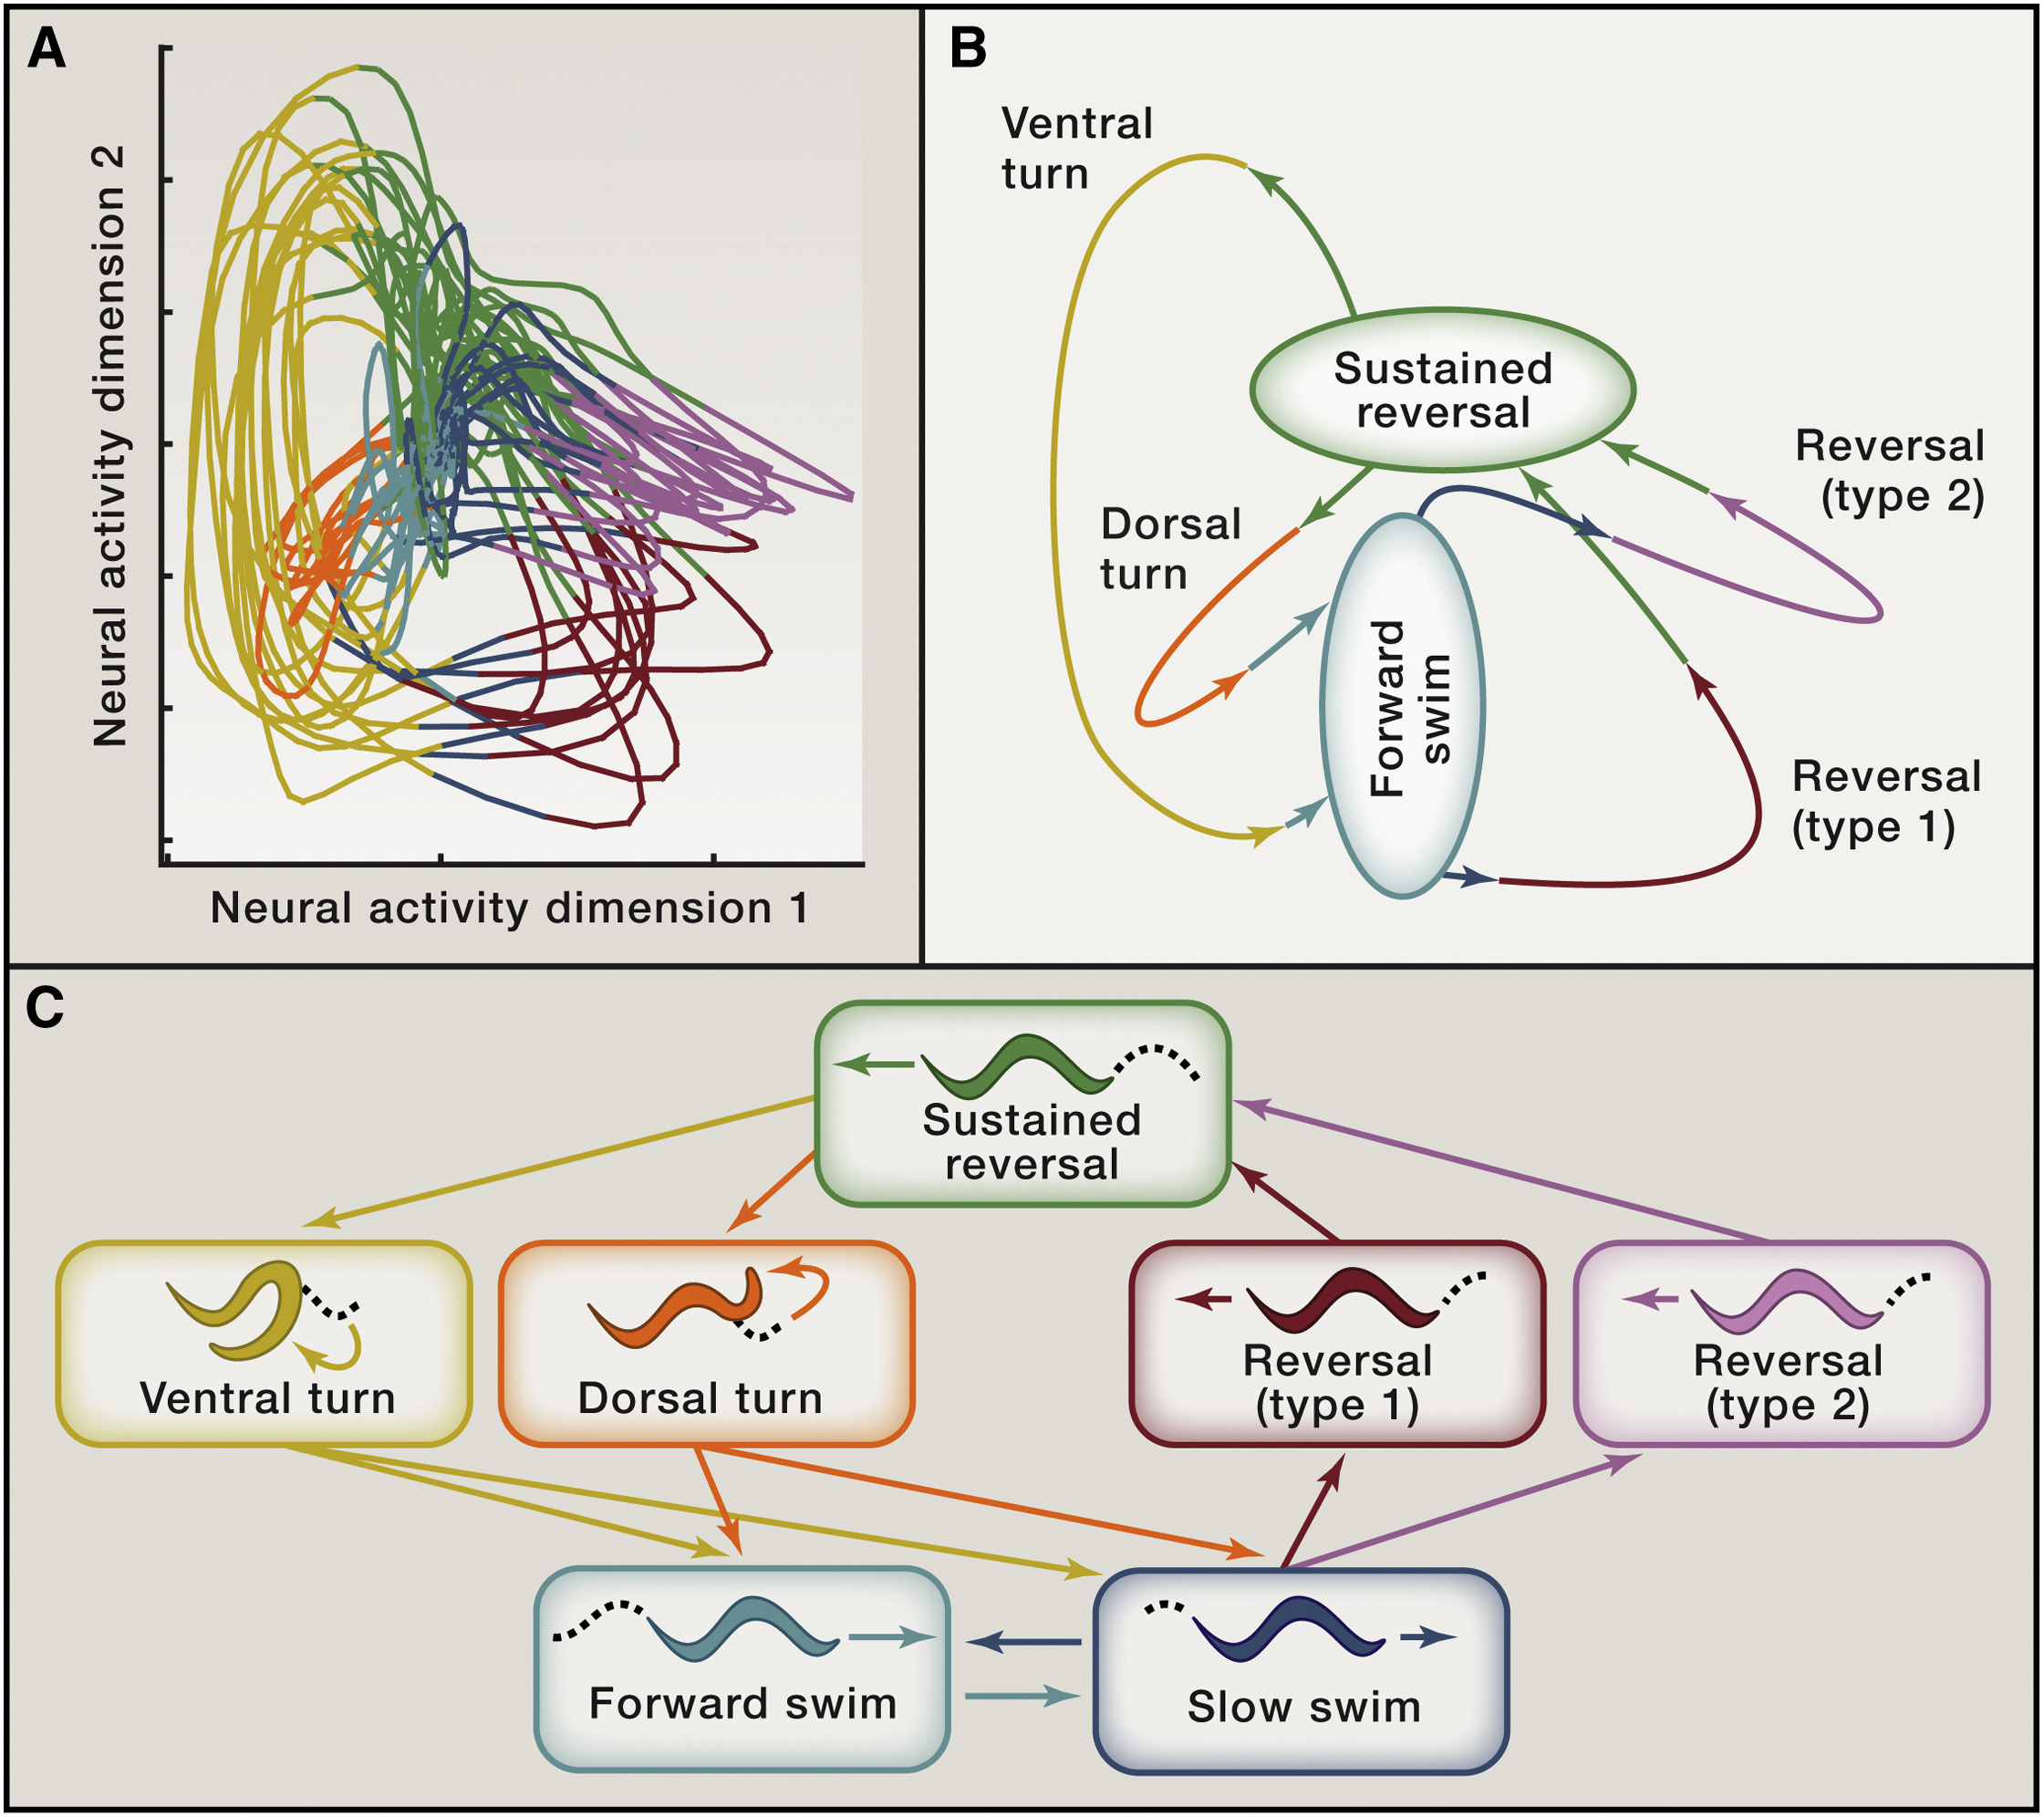
\includegraphics[width=\imsize]{kato_2.jpg}
	\caption[Representación de la Trayectoria de la Actividad Neuronal en C. elegans.]{ Representación de la Trayectoria de la Actividad Neuronal en C. elegans. (A) La trayectoria que ilustra la actividad neuronal, obtenida mediante imágenes que abarcan casi la totalidad del cerebro con una resolución celular en C. elegans, se proyecta en los dos primeros componentes principales. Esta dinámica presenta un patrón cíclico y estereotipado, donde la variación en el color identifica a qué grupo específico pertenece cada segmento de actividad neuronal. (B) En el espacio de actividad neuronal, se destacan regiones que se correlacionan con comportamientos específicos, indicando la relación entre la actividad neuronal y la locomoción observada. (C) Se presenta un diagrama de transición de estados que captura la dinámica de locomoción en C. elegans en paralelo con la actividad neuronal destacada en (B). Este diagrama arroja luz sobre la conexión entre la actividad neuronal y los comportamientos locomotores del gusano. (Adaptada de \protect\cite{branson_imaging_2015}). }\label{fig:kato1}
\end{figure}


Para validar estos resultados, Kato et al. llevaron a cabo un segundo conjunto de experimentos en los que obtuvieron imágenes de la actividad neuronal en gusanos que se comportaban libremente, mientras observaban simultáneamente la locomoción. Sorprendentemente, los grupos en el espacio de trayectoria neuronal, definidos únicamente en función de la actividad neuronal, se correlacionaban con diferentes comportamientos de locomoción, como avanzar, retroceder, girar y detenerse.


Por lo tanto, se infiere que una parte sustancial de la actividad neuronal en C. elegans, incluso en condiciones de inmovilidad, codifica el estado locomotor ficticio. El flujo de actividad neuronal (\Cref{fig:kato1}B) presenta similitudes con un diagrama de transición de estados de comportamiento  (\Cref{fig:kato1}C), una representación comúnmente utilizada para visualizar los tipos y probabilidades de transiciones de comportamiento observadas. Un rasgo sorprendente de estos patrones de actividad neuronal es que son en gran medida autogenerados. En conjunto, estos hallazgos sugieren que una parte sustancial del cerebro del gusano oscila constantemente entre estados que, cuando el animal se encuentra en movimiento libre, inducen distintos comportamientos de locomoción. La información sensorial modula las probabilidades de entrar y salir de estos estados, lo que podría explicar la variabilidad observada en el comportamiento de locomoción de C. elegans.




\subsection{Implementación Neural de Jerarquías Conductuales}\label{sec:kaplan}


La conducta es una secuencia de acciones ordenadas que los organismos llevan a cabo en el tiempo para interactuar con su entorno. Varias disciplinas, como la etología, la psicología y la neurociencia, han reconocido que muchos comportamientos, tanto innatos como adquiridos, presentan una estructura jerárquica que abarca múltiples niveles. Estos niveles van desde objetivos generales y estados conductuales hasta secuencias de acciones, subtareas y elementos motores específicos. La neurociencia contemporánea se enfrenta al desafío de profundizar en la comprensión de cómo el sistema nervioso controla y coordina estos niveles jerárquicos de comportamiento.

Para abordar este desafío, Kaplan et al. \cite{kaplan_nested_2020} llevaron a cabo una serie de experimentos que proporcionan información valiosa sobre la jerarquía espaciotemporal de dinámicas neuronales que abarcan todo el cerebro y la periferia de C. elegans durante su comportamiento locomotor  \cite{hollon_neural_2020}. Los mecanismos detallados de los circuitos descubiertos arrojan luz sobre cómo el sistema nervioso puede generar múltiples niveles de jerarquía conductual y coordinar sus interacciones para producir la salida motora en diferentes escalas temporales.


En su estudio, Kaplan et al.   caracterizaron por primera vez la locomoción en C. elegans como un proceso compuesto por varios niveles dentro de una jerarquía conductual (ver \Cref{fig:kaplan1}).  En el nivel superior, los gusanos se desplazan hacia adelante o hacia atrás, alterando su dirección de manera intermitente, aproximadamente cada 20 segundos. En el nivel intermedio, se encuentran las ondulaciones que se propagan a lo largo del cuerpo del gusano para impulsar su avance. Estas \textquote{curvas propagadas } inician su movimiento de la cabeza a la cola durante la locomoción hacia adelante y de la cola a la cabeza durante la locomoción hacia atrás, con un período de alrededor de 2 segundos. El nivel más bajo de la jerarquía conductual implica movimientos rápidos de la cabeza que ocasionalmente realizan los gusanos y que no se propagan completamente hasta la cola. Estos \textquote{lanzamientos de cabeza} de 1 segundo ocurren exclusivamente durante la locomoción hacia adelante, y su dirección está estrictamente ligada al ángulo de la última curva propagada, con lanzamientos de cabeza dorsales después de curvas dorsales y lanzamientos de cabeza ventrales después de curvas ventrales.




\begin{figure}[h!]
	\centering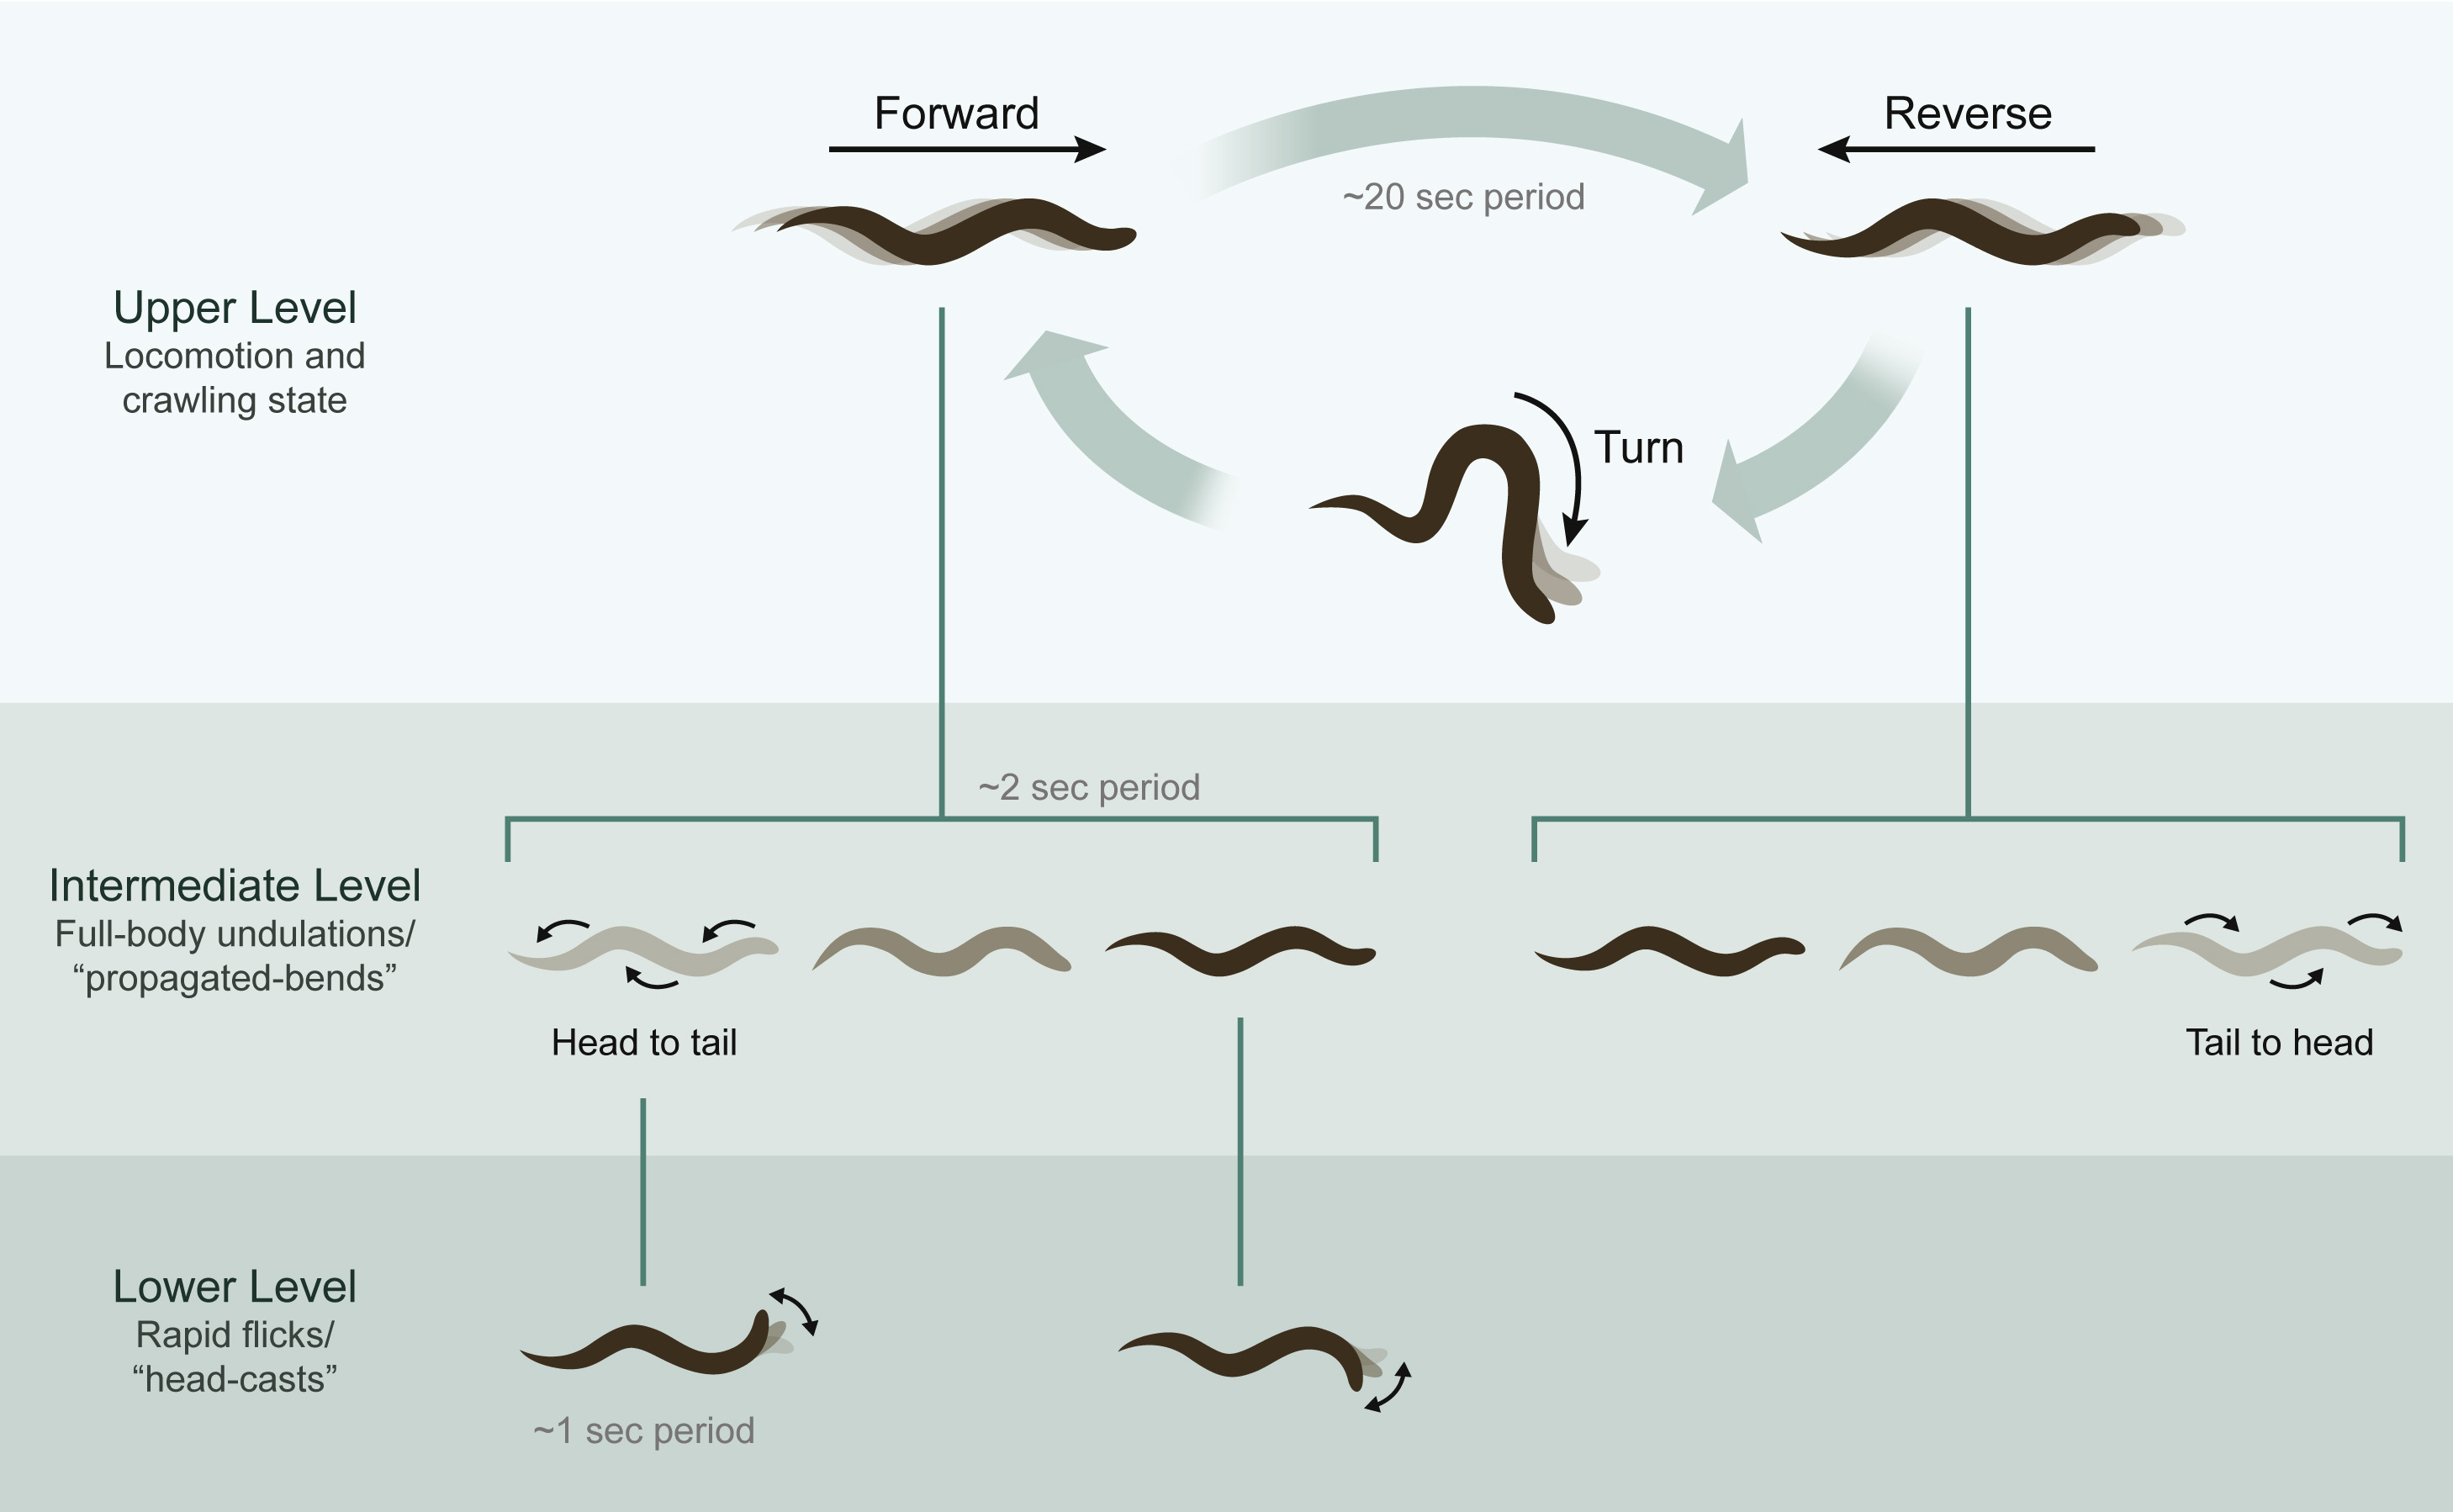
\includegraphics[width=\imsize]{kaplan1.jpg}
	\caption[Jerarquía Conductual en la Locomoción de C. elegans.]{ Jerarquía Conductual en la Locomoción de C. elegans. Esta representación visual nos permite observar cómo el comportamiento locomotor de C. elegans se organiza en distintos niveles jerárquicos, cada uno operando en escalas de tiempo específicas. La jerarquía conductual se refleja en la diferente duración de los comportamientos en C. elegans, lo que se traduce en distintas escalas de tiempo para cada nivel.	 (Figura adaptada de \protect\cite{hollon_neural_2020}). }\label{fig:kaplan1}
\end{figure}


Los experimentos de manipulación realizados por Kaplan et al.  indican que los diferentes niveles de la jerarquía de la locomoción en C. elegans están organizados de manera funcional jerárquica, con los niveles superiores ejerciendo influencia sobre los niveles inferiores, pero con una influencia limitada en la dirección opuesta. Es importante destacar que los patrones de actividad neuronal oscilatoria y su anidamiento jerárquico se mantuvieron incluso en animales físicamente inmovilizados, aunque a frecuencias generales más bajas, lo que sugiere que estas dinámicas rítmicas pueden persistir en gran medida independientemente de la retroalimentación propioceptiva. En conjunto, estos resultados respaldan la idea de que la organización jerárquica del comportamiento podría derivar, al menos en parte, de una organización intrínseca jerárquica de los circuitos de control motor.


\subsection{NeuroPAL: Un Avance en la Identificación Neuronal en C. elegans}


La adquisición y análisis de conjuntos de datos neuronales en C. elegans, como se ha detallado anteriormente, se han enfrentado a desafíos considerables, principalmente relacionados con la identificación precisa de neuronas en las imágenes microscópicas de estos organismos. En las investigaciones neurocientíficas con C. elegans, es común utilizar promotores de genes específicos para expresar la proteína verde fluorescente (GFP) con el propósito de determinar qué neuronas expresan dicho gen. Sin embargo, este enfoque se ha visto limitado por la identificación precisa de neuronas, ya que en muchas ocasiones, las neuronas adyacentes presentan morfologías similares y/o posiciones variables, lo que compromete la fiabilidad del proceso.

Para abordar este desafío, Yemini et al. \cite{yemini_neuropal_2021} han desarrollado la innovadora herramienta denominada \gls{NeuroPAL} (Neuronal Polychromatic Atlas of Landmarks).    El transgén NeuroPAL permite la expresión de diferentes combinaciones de cuatro proteínas fluorescentes distintas de la GFP en diversas neuronas de C. elegans. Este enfoque permite que las neuronas cercanas se iluminen con colores diferentes, lo que facilita su identificación de manera fiable (consulte la \Cref{fig:neuropal}). Las cuatro proteínas fluorescentes utilizadas en el NeuroPAL poseen espectros de excitación/emisión que las hacen fácilmente distinguibles entre sí y de la GFP. Como resultado, a través de sencillos cruces genéticos, es posible generar animales que portan tanto un transgén GFP como un transgén NeuroPAL, lo que, en principio, permite la identificación precisa de las neuronas que expresan GFP \cite{santiago_using_2022}.
 
La introducción de NeuroPAL ha supuesto un avance significativo en la identificación de neuronas en C. elegans, allanando el camino para un análisis más preciso y confiable de los datos neuronales. Esto, a su vez, ha contribuido al mejor entendimiento de la neurobiología de este modelo, fortaleciendo las bases para futuras investigaciones en este campo de estudio.

\begin{figure}[h!]
	\centering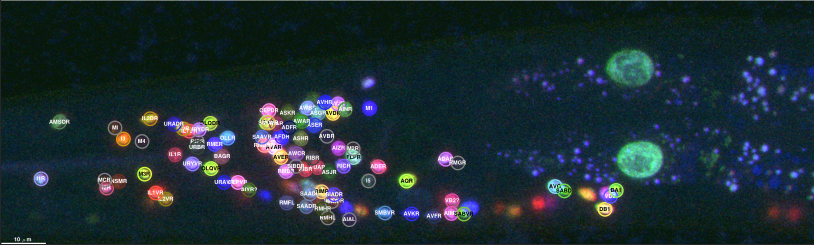
\includegraphics[width=\imsize]{neuropal.png}
	\caption[Visualización de la Actividad Neuronal en la Cabeza con NeuroPAL.	]{ Visualización de la Actividad Neuronal en la Cabeza con NeuroPAL.}\label{fig:neuropal}
\end{figure}


\section{Modelo de Procesamiento Sensoriomotor en C. elegans: Una Perspectiva Distribuida y Dinámica}\label{sec:modelo}

En esta sección, se presenta un modelo presente en la literatura que aborda la cuestión de cómo, desde una perspectiva neurobiológica, C. elegans podría llevar a cabo el procesamiento sensoriomotor. El propósito de este modelo es abordar la carencia teórica existente al integrar coherentemente los resultados previamente descritos relacionados con las conexiones neuronales (conectoma), los circuitos con funciones específicas y la dinámica neuronal a nivel global.  Este marco teórico proporcionará una base sólida para comprender la interacción entre la dinámica neuronal, el conectoma y el comportamiento en nuestro modelo robótico.


En investigaciones recientes, se ha avanzado hacia una visión más completa de cómo el sistema nervioso del C. elegans podría llevar a cabo cálculos y tomar decisiones en respuesta a las señales sensoriales recibidas. Estudios previos postulaban que la información fluía de manera predominantemente segregada y directa desde los circuitos sensoriales hacia los motores. Además, se clasificaban a las neuronas motoras en categorías dirigidas hacia los músculos de la cabeza o del cuerpo, mientras se identificaban cinco interneuronas premotoras como puntos neurales centrales en la red, recibiendo múltiples entradas de los circuitos sensoriales y funcionando como un cuello de botella en la transmisión de señales hacia las neuronas motoras del cuerpo  \cite{gray_circuit_2005} .  Esto sugiere una estrategia secuencial en la que la información sensorial de múltiples señales se integra en un grupo de interneuronas de la primera capa, que luego transmiten esta información, posiblemente transformada, a un grupo de interneuronas de la segunda capa. Estas últimas interconectan finalmente con las neuronas motoras de la cabeza y las interneuronas premotoras centrales para dirigir el comportamiento. La secuencia de procesamiento sensoriomotor se ilustra en la \Cref{fig:computosistema}.


\begin{figure}[h!]
	\centering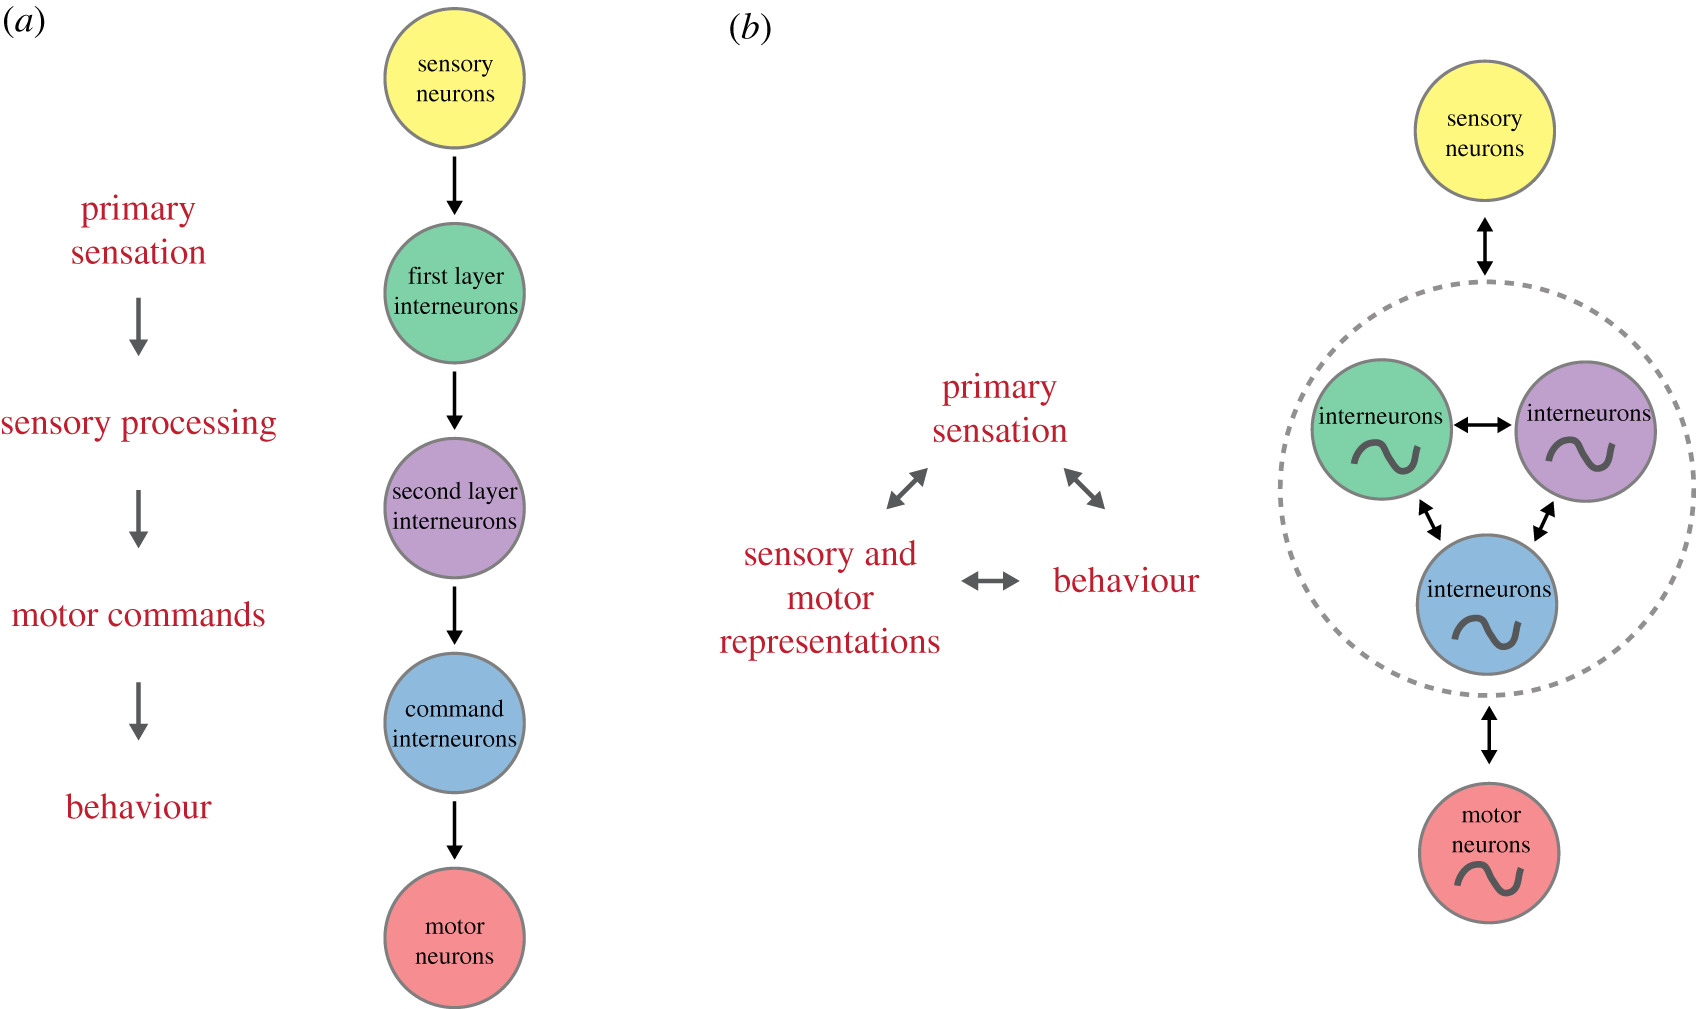
\includegraphics[width=\imsize]{sensioral.jpg}
	\caption[ Dos Modelos Contrastantes del Flujo Sensoriomotor en C. elegans.]{ Dos Modelos Contrastantes del Flujo Sensoriomotor en C. elegans. Dentro del contexto del procesamiento sensoriomotor en C. elegans, se contrastan dos modelos fundamentales  que representan enfoques diferentes para comprender cómo este organismo realiza estas funciones cruciales. El modelo (a), que denominamos \textquote{Modelos Secuenciales Segregados}, sugiere que la transformación de las representaciones sensoriales a las motoras sigue principalmente una ruta de alimentación directa y funcionalmente segregada a nivel de circuitos neuronales. En este enfoque, los cálculos se llevan a cabo en un orden temporal secuencial, con una clara distinción entre las etapas sensoriales y motoras. En contraste, el modelo (b), que llamaremos \textquote{Modelos Distribuidos}, es más consistente con los datos experimentales y propone una representación distribuida de las variables sensoriales y motoras a través de los circuitos neuronales. En este enfoque, se enfatiza la retroalimentación entre la mayoría de los elementos del sistema como una propiedad esencial. Las entradas sensoriales se integran de manera dinámica con la actividad interna de los circuitos neuronales, lo que permite que los cálculos se realicen de manera concurrente. En este modelo, las interacciones recíprocas dinámicas entre el cerebro, el cuerpo y el entorno son fundamentales para el procesamiento sensoriomotor.	  (Adaptada de \protect\cite{kaplan_sensorimotor_2018} ).}\label{fig:computosistema}
\end{figure}


No obstante, investigaciones más recientes han revelado una dinámica inesperada en la actividad de estas interneuronas. En lugar de actuar únicamente como mediadoras de la información sensorial, se ha observado que desempeñan un papel activo en la generación de comandos motores. Este hallazgo se sustenta en observaciones de animales inmovilizados, donde las actividades de las interneuronas se correlacionan de manera dinámica y coordinada. Las neuronas coactivas en estas grabaciones mantienen su actividad en un mismo estado motor, con escasas excepciones.

Kaplan et al. \cite{kaplan_sensorimotor_2018} postulan que el sistema nervioso del C. elegans se comprende mejor como un sistema distribuido y dinámico diseñado para generar comportamiento adaptativo. Esta red distribuida recibe entradas de neuronas sensoriales y ajusta su dinámica para la toma de decisiones. La  \Cref{fig:computosistema}B ilustra este procesamiento neuronal distribuido y dinámico. Los comandos motores se condensan eficientemente en el denominado colector de atractores, que representa una representación de baja dimensión de la actividad neuronal de alta dimensión, como se detalló previamente. Este colector se caracteriza por la participación de un gran número de neuronas, fuertes correlaciones y anti-correlaciones entre ellas, y una repetición cíclica de los estados de actividad de la red que involucra de manera consistente las mismas clases de neuronas en cada ciclo \cite{kato_global_2015}.


Un aspecto relevante es la suavidad del colector de atractores a nivel de la población neuronal en C. elegans, lo que implica una transición gradual en la actividad de la red (ver \Cref{fig:kato1}A). Esta característica es fundamental para ajustar las métricas del movimiento al cambiar entre diferentes patrones locomotores, similar a cómo se reduce gradualmente la velocidad de un vehículo antes de cambiar a la marcha atrás.

Para evaluar la hipótesis de codificación poblacional, se han desarrollado métodos computacionales avanzados \cite{elsayed_structure_2017}. Además, se espera que la obtención de imágenes del cerebro completo de gusanos en movimiento libre revele correlaciones entre características poblacionales y comportamiento. En última instancia, la actividad altamente correlacionada y consistente de la red subyace en los comandos motores en el C. elegans.


Kaplan et al. \cite{kaplan_sensorimotor_2018} plantean que esta característica contribuye a la producción robusta del comportamiento, proporcionando una columna vertebral preconfigurada que persiste bajo flujos complejos de entradas multisensoriales, como las que los gusanos encuentran en su entorno natural del suelo. Las interneuronas desempeñan un papel crucial en este proceso debido a su conectividad excepcional, formando un \textquote{club rico} \cite{cook_whole-animal_2019}. Se sugiere que las probabilidades de transición en el colector de atractores dependen de la dinámica interna y de una función ponderada de las entradas sensoriales a las interneuronas, lo que explicaría la redundancia en los patrones de actividad relacionados con los comandos motores de diferentes interneuronas. Estas interneuronas no son redundantes, sino canales que diferencian las entradas en una red distribuida de comandos motores, influyendo en la dinámica en curso. 



\section{Integración de Modelos Robóticos y Neurobiología en C. elegans para la Investigación en Neuro-robótica}
\label{sec:neurorobot}
En esta apartado, se examinan  los modelos robóticos documentados en la literatura que buscan integrar los componentes previamente descritos: el conectoma, la función neuronal y el comportamiento del nematodo C. elegans.

En las últimas décadas, hemos sido testigos de avances significativos en el desarrollo de técnicas de inteligencia artificial (IA) para su aplicación en la robótica. A pesar de estos notables logros, subsisten limitaciones críticas en términos de generalización, aprendizaje y robustez en las soluciones implementadas. Para abordar estas limitaciones, ha emergido un enfoque prometedor: el estudio de sistemas biológicos. La comprensión de la relación entre el comportamiento y el procesamiento de la información en los circuitos neuronales constituye un desafío central en el campo de la neurociencia. Asimismo, esta comprensión puede sentar las bases para el desarrollo de algoritmos inspirados en los principios neuronales, con aplicaciones en la robótica \cite{norman-tenazas_worminator_2018}.


Un aspecto crítico para llevar a cabo la simulación de un sistema nervioso completo radica en la disponibilidad del conectoma de dicho sistema. Como se discutió en el \Cref{sec:conectoma} el conectoma se concibe convencionalmente como un grafo que constituye un objeto matemático compuesto por vértices, bordes dirigidos y atributos. La construcción de conectomas a partir de microscopía electrónica da lugar a gráficos anatómicos, donde los vértices representan neuronas individuales y los bordes representan conexiones sinápticas dirigidas.


La simulación de circuitos neuronales también conlleva la necesidad de una comprensión profunda de la dinámica neuronal y la neuromodulación, ya que diferentes dinámicas temporales neuronales pueden resultar en diferentes respuestas a partir del mismo conectoma subyacente. C. elegans, como organismo modelo, constituye una base sólida para la simulación en circuito cerrado del comportamiento. Su conectoma se caracteriza con gran detalle, si bien persisten incógnitas en relación a la dinámica neuronal y al papel de la neuromodulación. A pesar de ello, se han propuesto circuitos neuronales que explican una variedad de comportamientos observables, como la retracción al tacto y la exploración de entornos \cite{bargmann_chemosensation_2006}.


En este contexto, el proyecto OpenWorm ha desarrollado una simulación detallada que abarca todas las células relevantes del nematodo C. elegans, involucradas en procesos de detección y actividad motora \cite{sarma_openworm_2018}. Estas simulaciones se basan en modelos que describen la dinámica de los canales neuronales.

Además, investigaciones recientes han comparado la respuesta de retracción al tacto del gusano con políticas de control óptimas \cite{lechner_worm-level_2017}, y se ha propuesto un modelo de Simulink del gusano que se fundamenta en modelos de un solo compartimento. Otro enfoque consiste en la implementación de simulaciones dinámicas del conectoma de C. elegans en plataformas físicas y robóticas. Estos estudios aplican principios computacionales neuronales inspirados en el comportamiento de C. elegans al control de robots, lo que permite la comparación entre algoritmos basados en la biología y enfoques convencionales. Un ejemplo de ello es una plataforma robótica que ha implementado una simulación de seis neuronas relacionadas con la quimiotaxis de C. elegans \cite{morse_robust_1998}, aunque no ha simulado todo el sistema nervioso del gusano.

Recientemente, Timothy Busbice \cite{Timothy_robot}  ha desarrollado un modelo de red neuronal utilizando el conectoma completo del nematodo C. elegans como sustrato (consultar Figura 2.11). Este modelo de red neuronal se ha empleado para el control de un vehículo robot. La actividad de las neuronas sensoriales se estimuló mediante lecturas de un sensor de posición, y las salidas de las neuronas motoras del modelo se utilizaron para el control de los motores del robot. El comportamiento resultante, en el que el robot exploró su entorno y eludió obstáculos, surgió de manera espontánea a partir de la interacción del modelo de red neuronal con el entorno (\url{https://www.youtube.com/watch?v=YWQnzylhgHc}).




\begin{figure}[h!]
	\centering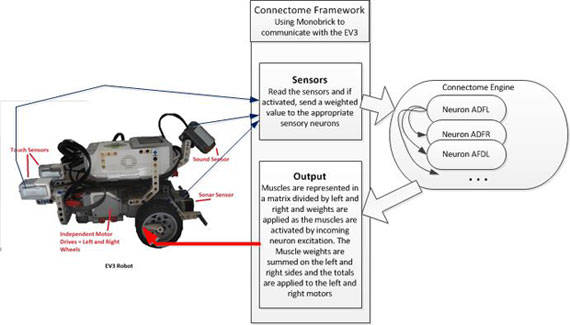
\includegraphics[width=\imsize]{connectomerobot.jpg}
	\caption[ Interacción Entre Sensores y Neuronas Motoras en el Robot de Timothy Busbice.]{  Interacción Entre Sensores y Neuronas Motoras en el Robot de Timothy Busbice. En esta figura se representa la interacción entre los sensores del robot construido por Timothy Busbice utilizando el Lego Mindstorms EV3 y el conectoma simulado del nematodo C. elegans. Un programa de entrada es responsable de activar las neuronas sensoriales correspondientes en el conectoma simulado en respuesta a las lecturas de los sensores del robot. Por otro lado, un programa de salida recopila las señales de las neuronas motoras y calcula valores ponderados que se utilizan para controlar las ruedas del robot, lo que resulta en su movimiento.  (Adaptada de \protect\cite{Timothy_robot} ).}\label{fig:timoty}
\end{figure}



Finalmente, inspirado en el trabajo de Timothy, Nathan Griffith ha concebido el proyecto \textquote{Nematoduino}, una simulación robótica del nematodo C. elegans compatible con Arduino Uno (El código esta disponible en \url{https://github.com/nategri/nematoduino}). Este proyecto se basa en un modelo de redes neuronales que utiliza un esquema de \textquote{leaky integrate-and-fire} del gusano biológico.  La implementación se caracteriza por una representación comprimida del conectoma (8 kilobytes) y la capacidad de ejecutarse en la plataforma económica y ampliamente disponible de Arduino Uno. A pesar de que el software \textquote{Nematoduino} consume una parte sustancial de la memoria y recursos del Arduino Uno, aún deja espacio para la personalización y experimentación. Con ruedas y un sensor de proximidad conectado a la placa, Nathan ha logrado imitar los movimientos y respuestas del gusano, como se puede apreciar en un video disponible en línea (\url{https://www.youtube.com/watch?v=u406m-v4Y3Y}).

Los esfuerzos en el campo de la neuro-robótica representan avances emocionantes al aplicar la biología computacional al diseño y control de sistemas robóticos, lo que podría tener un impacto significativo en el desarrollo de sistemas autónomos inspirados en la naturaleza, aspecto central en esta investigación doctoral.




\section{Discusión}



En este capítulo de la tesis, se presentan los fundamentos neurobiológicos del C. elegans, desde los experimentos realizados a nivel de toda la población neuronal, un modelo que integra la relación entre topología, función y comportamiento, hasta los modelos neurorrobóticos que podrían implementar físicamente estas características. Basándonos en el marco teórico anterior, en esta sección se presentan las preguntas que se desean resolver en los capítulos siguientes de esta parte de la tesis.

El nematodo Caenorhabditis elegans es un sistema modelo manejable para estudiar la locomoción, la navegación sensorial y la toma de decisiones. En su hábitat natural, se cree que navega por entornos multisensoriales complejos para encontrar comida y parejas sexuales, mientras evita amenazas como depredadores o entornos tóxicos. Si bien la investigación de las últimas décadas ha arrojado mucha luz sobre las funciones y los mecanismos de neuronas sensoriales seleccionadas, estamos al borde de comprender cómo la información sensorial es integrada por circuitos de interneuronas para la selección de acciones en el gusano. Los avances tecnológicos recientes han permitido la obtención de imágenes de \ce{Ca^{2+}} de todo el cerebro y de la actividad neuronal en gusanos que se mueven libremente.


Los animales que navegan por un entorno complejo no se limitan a reproducir los estímulos externos a través de sus acciones, sino que moldean su comportamiento en función de las condiciones. Los circuitos de quimiotaxis pueden transformar las entradas sensoriales suaves o ruidosas en reorientaciones discretas y probabilísticas. De manera más general, los animales toman decisiones y exploran entornos a través de acciones discretas y mutuamente excluyentes, que también son la base de paradigmas conductuales experimentales como las decisiones de ir/no ir o de elección forzada \cite{frederick_characterizing_2011}. Se hipotetiza que tanto las representaciones neuronales oscilatorias como las distribuidas son estrategias organizativas neuronales fundamentales, sobre las que quedan numerosas preguntas abiertas.

¿Cómo se relaciona el estado de actividad neuronal con el comportamiento? ¿Cómo se generan los patrones cíclicos y cómo coordinan su actividad las muchas neuronas de esta red? ¿Cuáles son las ventajas de estas implementaciones? ¿Cómo se integran la información sensorial, el aprendizaje y la historia del animal para cambiar la representación neuronal? Los experimentos presentados en los \Cref{sec:kato,sec:kaplan} respondieron a las anteriores preguntas al demostrar que la organización del comportamiento en el gusano está codificada en una estructura jerárquica de dinámica neuronal globalmente distribuida, continua y de baja dimensión, lo que lleva a la conclusión de que los estados de comportamiento están codificados en el cerebro como una representación interna que emerge del cerebro.

Para evaluar cómo se genera una actividad dinámica sostenida y de baja dimensión, es fundamental comprender el papel que juega el connectoma en la generación de movimiento rítmico. La estructura de la conectividad de una red neuronal a menudo determina cómo opera la red en su conjunto, codificando respuestas conductuales clave caracterizadas por patrones de actividad de baja dimensión. Sin embargo, la importancia exacta de la conectividad específica de una red no está clara, y la dinámica de la red neuronal a menudo se modela computacionalmente utilizando redes aleatorias uniformes. En C. elegans, sin embargo, la estructura del connectoma claramente no es aleatoria y puede desempeñar un papel crítico adicional en ayudar a generar o facilitar respuestas rítmicas. Esto se sugiere por el hecho de que los modelos computacionales del connectoma pueden generar oscilaciones de neuronas motoras relacionadas con la locomoción hacia adelante en respuesta a estímulos constantes, incluso sin propiocepción (e incluso cuando se modelan solo las dinámicas neuronales, sin modelado muscular, corporal o ambiental acoplado). Esto sugiere que las respuestas oscilatorias y estereotipadas están, en algún nivel, codificadas dentro del connectoma.


Por otro lado, la arquitectura de cableado de las redes neuronales se considera un determinante importante de sus cálculos dinámicos. Por lo tanto, un esfuerzo continuo en neurociencia es generar connectomas completos con resolución de sinapsis junto con mapas de actividad de todo el cerebro. Sin embargo, la relación estructura-función, es decir, cómo se relacionan el connectoma anatómico y la dinámica neuronal entre sí a escala global, sigue sin resolverse. Uzel et al. \cite{uzel_set_2022} compararon sistemáticamente las características de los grafos en el connectoma de C. elegans con las correlaciones en la dinámica neuronal de todo el sistema nervioso y encontraron que pocos motivos de conectividad local y principalmente otras características no locales, como los motivos de tripletes y las similitudes de entrada, pueden predecir relaciones funcionales entre neuronas. Sorprendentemente, cantidades como la fuerza de la conexión y la cantidad de entradas comunes no mejoran estas predicciones, lo que sugiere que la topología de la red es suficiente. Esto demuestra que las neuronas centrales en el connectoma son clave para estas características topológicas relevantes. De manera consistente, la inhibición de múltiples neuronas centrales interrumpe específicamente las correlaciones de todo el cerebro. Por lo tanto, los autores proponen que un conjunto de neuronas centrales y características de conectividad no locales proporcionan un sustrato anatómico para la dinámica cerebral global.


En los últimos años, el estudio de sistemas neuronales ha incorporado un nuevo paradigma que integra todo lo anteriormente expuesto, donde se considera la relación entre la información que procesa el cerebro, el cuerpo de los individuos y su interacción con el medio ambiente. Según este enfoque, el procesamiento de la información no puede considerarse de forma aislada en el cerebro, sino que debe hacerlo incorporando el estado dinámico del medio ambiente y cómo este es percibido por los diferentes sentidos propios de cada especie \cite{der_playful_2012}. Al mismo tiempo, otro de los grandes interrogantes en el estudio de las ciencias cognitivas y la inteligencia artificial está vinculado a la motivación que tienen los organismos para actuar de forma espontánea y cómo pueden diseñarse sistemas artificiales que actúen con una intención u objetivo sin que este tenga que estar programado de forma explícita \cite{brembs_towards_2010}.   Este paradigma resalta la importancia de estudiar el sistema nervioso, el cuerpo y el medio ambiente como un sistema acoplado, con el fin de comprender las propiedades que emergen de su interacción dinámica continua \cite{webb_robots_2002, floreano_robotics_2014}.  En este contexto, el uso de robots aparece como una herramienta de modelado atractiva, ya que es posible acceder y tener control total sobre los parámetros y variables dinámicas que gobiernan su comportamiento \cite{pfeifer_self-organization_2007}. Además, la implementación física de un robot permite probar el desempeño de algoritmos en un cuerpo sujeto a las leyes de la física e inmerso en tiempo real en un entorno natural, evitando así los complejos tecnicismos de la simulación del entorno, procedimiento que involucra sus propios modelos y, por lo tanto, agrega más variables, suposiciones y ruido al análisis. A su vez, esto nos permite centrarnos directamente en la dinámica global que emerge del connectoma y cómo afecta el comportamiento.


Tanto los resultados experimentales de Kato et al. \cite{kato_global_2015}, que muestran que la dinámica de la red interactúa con las neuronas sensoriales desde la primera sinapsis, proporcionando un andamiaje sólido para que las entradas sensoriales modulen el comportamiento, como los hallazgos del modelo del procesamiento sensoriomotor de Kaplan et al. \cite{kaplan_sensorimotor_2018}(\Cref{sec:modelo}) que muestran que la integración sensoriomotora en C. elegans ocurre de manera dinámica y distribuida, sugieren que la integración concurrente y distribuida de la dinámica sensorial y motora es un principio fundamental del funcionamiento del sistema nervioso. Por lo tanto, proponemos a C. elegans como un modelo manejable para estudiar las funciones y las ventajas computacionales de estas interacciones cerebro-cuerpo-entorno.

 Como se mencionó en el \Cref{sec:neurorobot}, Timothy Busbice, en línea con lo anterior, construyó un modelo de red neuronal utilizando como sustrato la información del connectoma del nematodo C. elegans. El robot presenta comportamientos emergentes que le permiten navegar espontáneamente cuando se estimulan las neuronas sensoriales asociadas con la presencia de alimentos y retroceder cuando se estimulan las neuronas de toque de la nariz al enfrentar un obstáculo. Es importante enfatizar que este comportamiento no fue programado intencionalmente en el robot, sino que surgió espontáneamente a partir del modelo de red neuronal y la interacción del robot con el medio ambiente.
 
 Pero ¿cómo emerge este comportamiento? Como objetivo general de esta parte de la tesis, buscaremos responder a este interrogante analizando las relaciones entre la estructura de red, la dinámica neuronal y el comportamiento emergente. Por tanto, el modelo robótico constituye una excelente plataforma para estudiar la interacción entre el connectoma, la dinámica neuronal y los comportamientos emergentes. Sin embargo, hasta ahora no se ha analizado ni la dinámica global del modelo ni su correlación con el connectoma subyacente y las acciones emergentes del robot.
 
 

 
 El primer objetivo específico busca cuantificar los comportamientos que emergen de un vehículo robótico que está controlado por una simulación numérica de red neuronal basada en el connectoma de C. elegans. En la simulación, las neuronas tienen el mismo umbral de activación y, en consecuencia, tienen una dinámica idéntica a la de las unidades aisladas. De esta manera, los cambios observados en su dinámica reflejan sus interacciones a través de la distribución no uniforme de la conectividad sináptica. Esto nos permite analizar la dinámica neuronal que emerge a través del connectoma y, al mismo tiempo, estudiar la interacción entre la dinámica neuronal y las acciones del robot. Esto proporciona una metodología para comprobar si las interacciones del circuito son suficientes para explicar el comportamiento o se necesitan más suposiciones. Primero reproduciremos los resultados publicados en C. elegans \cite{busbice_extending_nodate}. Luego analizaremos los comportamientos que emergen al manipular los circuitos más importantes del organismo real, asociados a la locomoción y la quimiosensación. La hipótesis de trabajo es que al implementar los circuitos funcionales en la red neuronal del robot, el robot tendrá comportamientos emergentes semejantes a los del organismo real.
 
 Al utilizar un modelo computacional para la dinámica del connectoma de C. elegans, proporcionamos un fuerte apoyo teórico y computacional para la hipótesis de que la propiocepción dentro de las neuronas motoras sí codifica e impulsa la actividad rítmica. El segundo objetivo busca caracterizar si algunos aspectos básicos de los comportamientos motores observados en el C. elegans están determinados por la estructura subyacente de la red neuronal asociada. Apoyados en estudios recientes que han demostrado que las redes biológicas, como el connectoma de C. elegans, tienen propiedades de redes complejas como mundo pequeño, caminos cortos entre dos nodos cualquiera, conexiones altamente agrupadas y principalmente motivos de red que podrían permitir procesamiento computacional canónico en números significativamente superiores a los de las redes aleatorias, proponemos la hipótesis de que esas características de red compleja, junto con una dinámica neuronal adecuada, permiten un comportamiento emergente, a diferencia de una red aleatoria que no tiene complejidad.
 
 El objetivo del experimento es comprobar que la estructura topológica de la red neuronal es necesaria para el comportamiento complejo del robot y no es un epifenómeno. Para corroborar esta hipótesis, se implementarán connectomas aleatorios en el robot para contrastar su resultado con el de la implementación con C. elegans.
 
 El tercer objetivo específico busca comprender cómo un sistema nervioso codifica, organiza y secuencia comportamientos. Se quiere ver si la dinámica neuronal global del gusano tiene la presencia de grupos de neuronas sincronizadas con una dinámica global de baja dimensión cíclica y estereotipada, como lo documentado en C. elegans reales. Para lograr esto, se realizarán experimentos monitorizando la dinámica neuronal global y aplicando las mismas técnicas que Kato et al. al conjunto de datos de la dinámica neuronal simulada. La hipótesis de trabajo es que en el robot se encontrará una actividad de red coordinada, al igual que en el organismo, como consecuencia de que la computación del comportamiento motor está implementada en el connectoma de C. elegans, tal como lo sugiere el modelo de Kaplan et al. (\Cref{sec.modelo})
 
 
 El cuarto objetivo específico busca comprender si la dinámica neuronal global del neurorobot también presenta una estructura jerárquica en los circuitos cerebrales y motores, donde las dinámicas más lentas limitan el estado y la función de las más rápidas, tal como en los experimentos en C. elegans. Nuestra hipótesis es que, a pesar de que todas las neuronas tienen el mismo umbral de activación y, por tanto, tienen una dinámica individual idéntica a la de las unidades aisladas, esperamos que su dinámica refleje la distribución no uniforme de la conectividad sináptica, dando como resultado una estructura jerárquica de frecuencias.
 
 En el siguiente capítulo se mostrarán los aspectos técnicos para la implementación de la dinámica neuronal de C. elegans en un robot. Se presentará el modelo de dinámica neuronal propuesto, los dos robots que implementarán esta dinámica y, finalmente, los métodos que se aplicarán sobre el resultado del comportamiento. El desarrollo de esta parte de la tesis tiene un alto impacto a nivel general, ya que intenta comprender la relación entre comportamientos emergentes en sistemas biológicos y la dinámica y estructura del cerebro, partiendo de un enfoque original que incorpora elementos de neurociencia experimental (connectomas), biología computacional (dinámica neuronal), sistemas complejos (comportamientos emergentes) y robótica (Arduino, Raspberry Pi). Este enfoque innovador abre la puerta a aspectos que nunca antes han sido considerados y se encontraron resultados novedosos, relevantes para el conocimiento científico en general y con alto impacto en todas estas áreas. Solo si podemos simular y manipular racionalmente un sistema nervioso, podremos comenzar a comprenderlo de verdad. Una vez más, el diminuto gusano de Brenner, que ocupa su lugar dulce único entre la simplicidad y la complejidad, se encuentra en la primera línea de los problemas más desafiantes de la biología.
 
 
\subsection{Hipótesis y Objetivos}
 
 \subsubsection{Hipótesis General}
 
 Se postula que la dinámica neuronal del nematodo C. elegans, basada en su connectoma, es un principio fundamental para el comportamiento emergente. Además, esta dinámica neuronal es replicable en un robot controlado por una red neuronal simulada, lo que permitirá comprender la relación entre el connectoma, la dinámica neuronal y los comportamientos emergentes.
 
 \subsubsection{Hipótesis Específica 1:}
 
 Se plantea que la implementación de circuitos funcionales del C. elegans en la red neuronal de un robot conducirá a comportamientos emergentes similares a los observados en el organismo real, respaldando la idea de que la propriocepción dentro de las neuronas motoras codifica e impulsa la actividad rítmica.
 
 \subsubsection{Hipótesis Específica 2:}
 
 Se sugiere que la estructura topológica de la red neuronal es un factor crítico para el comportamiento complejo del robot, en contraste con las redes aleatorias, lo que implica que las propiedades de redes complejas del connectoma de C. elegans son esenciales para el procesamiento computacional y el comportamiento emergente.
 
 \subsubsection{Hipótesis Específica 3:}
 
 La hipótesis sostiene que la dinámica neuronal global del robot mostrará una actividad de red coordinada, similar a la observada en C. elegans reales, debido a que la computación del comportamiento motor se basa en el connectoma del nematodo, según el modelo de Kaplan et al. \cite{kaplan_sensorimotor_2018}
 
 \subsubsection{Hipótesis Específica 4:}
 
 Se plantea que la dinámica neuronal global del neurorobot revelará una estructura jerárquica en los circuitos cerebrales y motores, donde las dinámicas más lentas limitan el estado y la función de las más rápidas, en concordancia con los experimentos en C. elegans.
 
 
 \subsection{Objetivos Generales y Específicos}
 
 Para abordar esta hipótesis general, se han formulado varios objetivos específicos:
 
 \subsection{Objetivo General}
 
 El propósito principal de esta investigación es comprender la relación entre el connectoma, la dinámica neuronal y los comportamientos emergentes, utilizando el nematodo C. elegans como modelo y replicando esta dinámica en un robot controlado por una red neuronal simulada.
 
 \subsubsection{Objetivo 1: Cuantificar Comportamientos Emergentes}
 
 El primer objetivo específico consiste en cuantificar los comportamientos emergentes en un vehículo robótico controlado por una simulación de red neuronal basada en el connectoma de C. elegans. Esto nos permitirá demostrar que la propriocepción dentro de las neuronas motoras codifica la actividad rítmica, respaldando así la hipótesis de trabajo.
 
 \subsubsection{Objetivo 2: Caracterizar la Estructura Topológica}
 
 El segundo objetivo específico se centra en caracterizar la importancia de la estructura topológica de la red neuronal en la generación de comportamientos complejos en el robot. Esto implica comparar la implementación de connectomas aleatorios con la del connectoma de C. elegans para corroborar la relevancia de las propiedades de redes complejas.
 
 
 \subsubsection{Objetivo 3: Analizar la Dinámica Neuronal Global}
 
 El tercer objetivo específico busca analizar la dinámica neuronal global del robot, examinando la presencia de grupos de neuronas sincronizadas con una dinámica de baja dimensión cíclica y estereotipada. Esto se hará en concordancia con los hallazgos en C. elegans y nos ayudará a comprender mejor la dinámica de la red neuronal.
 
 \subsubsection{Objetivo 4: Estudiar la Estructura Jerárquica de los Circuitos Cerebrales y Motores}
 
 El cuarto objetivo específico se enfoca en investigar si la dinámica neuronal global del neurorobot exhibe una estructura jerárquica en los circuitos cerebrales y motores. Esto incluye la evaluación de cómo las dinámicas más lentas limitan el estado y la función de las más rápidas, siguiendo los patrones observados en los experimentos con C. elegans.  
 
 Estos objetivos específicos se alinean con la hipótesis general y proporcionan un enfoque integral para la investigación. Cada objetivo contribuye a una comprensión más profunda de la dinámica neuronal y el comportamiento emergente en C. elegans y su replicación en un entorno robótico controlado por una red neuronal simulada. El estudio interconectado de estos objetivos nos permitirá avanzar hacia una comprensión más completa de la relación entre el connectoma, la dinámica neuronal y los comportamientos emergentes en estos sistemas biológicos y robóticos.
 
 
 




\chapter{Métodos y montaje experimental}\label{cap:modeloneuronal_robot}
\graphicspath{{figs/capitulo_modelo_dinamica_neuronal/}}

\chapterquote{We shall assume. . .\\
	. . . that all cows are spherical.
}{old joke}


En el capítulo anterior, se sentaron los fundamentos, tanto biológicos como conceptuales, que sustentan el entendimiento de la dinámica neuronal global en C. elegans. La disponibilidad de grabaciones neuronales a gran escala en organismos modelo ha transformado profundamente nuestras capacidades para llevar a cabo modelizaciones teóricas de la dinámica de poblaciones neuronales. Los recientes avances en tecnologías de imagen de todo el cerebro para el nematodo C. elegans \cite{kato_global_2015}, han desbloqueado la posibilidad de estudiar de manera integral la relación entre la actividad neuronal y los resultados conductuales. Es crucial destacar que C. elegans se presenta como un modelo excepcional que permite cuantificar la dinámica de poblaciones neuronales, ya que cuenta únicamente con 302 neuronas, cuya conectividad electrofisiológica estereotipada (conectoma) se ha detallado minuciosamente a través de microscopía electrónica de secciones seriadas\cite{cook_whole-animal_2019}.


En este contexto, el propósito de esta sección de la tesis es dilucidar cómo se manifiesta el comportamiento en un robot en el que se ha implementado la dinámica neuronal de C. elegans. Este enfoque nos conduce hacia una comprensión más profunda de cómo el sistema nervioso de C. elegans podría llevar a cabo cálculos y tomar decisiones en respuesta a las señales sensoriales que recibe. De acuerdo a la proposición de Kaplan et al., el sistema nervioso del gusano se comprende de mejor manera como un sistema distribuido y dinámico diseñado para generar un comportamiento adecuado, implicando la mayoría de las interneuronas y neuronas motoras. Esta red distribuida recibe entradas de neuronas sensoriales que actúan para modificar su dinámica con el fin de tomar decisiones. De esta forma, el conectoma funciona como una estructura análoga a la arquitectura de una computadora biológica, que, en conjunto con una dinámica neuronal apropiada, posibilita la emergencia del comportamiento.


En la investigación científica, los modelos y simulaciones juegan un rol esencial, proporcionando herramientas valiosas para validar observaciones y teorías relacionadas con las causas subyacentes de comportamientos específicos. No obstante, es vital reconocer que la modelización o simulación de comportamientos específicos puede derivar en interpretaciones sesgadas si no se considera el organismo en su totalidad. No siempre resulta obvio que una pequeña parte del organismo producirá los mismos resultados al incorporar más componentes del organismo al modelo. Para abordar estas limitaciones, en esta sección de la tesis se introduce un robot impulsado por una simulación que abarca todo el conectoma. Además, se proporciona un marco experimental que ilustra cómo se puede aprovechar la no linealidad para crear un modelo global de la dinámica de las poblaciones neuronales y cómo este enfoque puede aplicarse de manera sencilla a organismos modelo más complejos.


Este capítulo también detalla las metodologías utilizadas para comprender cómo se ensamblan las dinámicas de la red y cómo la estructura de la red, en conjunto con las conexiones sinápticas, generan las dinámicas observadas. Dado que los registros de la dinámica neuronal de todo el cerebro en C. elegans proporcionan datos de alta dimensión (datos de series de tiempo de alrededor de 300 neuronas), se torna esencial extraer información relevante mientras se reduce la dimensionalidad de los datos. Esta sección en su conjunto forma un enfoque holístico y coherente para abordar el problema de la dinámica neuronal en C. elegans y su aplicación a modelos más complejos en la investigación científica.




\section{Modelo de dinámica  neuronal}\label{sec:modelo_dinamica_neuronal}



En el transcurso de la locomoción animal, los organismos se ven inmersos en un continuo flujo de señales sensoriales provenientes de su entorno. Por lo tanto, resulta imperativo que los sistemas nerviosos de estos seres vivos sean capaces de discernir información relevante para la conducta, permitiéndoles generar respuestas adaptativas frente a estos estímulos. La comprensión de cómo los circuitos sensoriomotores procesan estas señales de manera adaptable, considerando factores como el contexto y la experiencia, ha sido objeto de una extensa investigación en las últimas décadas \cite{flavell_dynamic_2022}.

En este contexto, la modelización computacional emerge como una herramienta de gran potencial para investigar y comprender el procesamiento de información en sistemas neuronales. Estos modelos desempeñan un papel central en la desentrañación de los mecanismos subyacentes a la transmisión sináptica, el potencial de acción, la integración dendrítica y, más recientemente, la función de los circuitos neuronales. A pesar de la diversidad de estos modelos en cuanto a su nivel de detalle biológico, que va desde simplificaciones de alto nivel que arrojan luz sobre el comportamiento global de los circuitos, hasta modelos biológicamente detallados que permiten explorar en detalle los mecanismos subyacentes a la función de los circuitos, es importante destacar que los modelos biológicamente detallados a menudo se caracterizan por su intrincación y la inclusión de numerosos parámetros. Sin embargo, a pesar de la abundancia de datos experimentales procedentes del mapeo del conectoma, la cartografía de la actividad funcional y las iniciativas a gran escala relacionadas con el cerebro, la confianza en las predicciones de estos modelos suele verse limitada por su complejidad y la percepción de falta de restricción \cite{gleeson_open_2019}.



En lo que respecta al C. elegans, se han desarrollado modelos en varios niveles de complejidad \cite{gleeson_c302_2018}. Estos abarcan desde modelos de neuronas individuales \cite{kuramochi_computational_2017} y músculos \cite{boyle_caenorhabditis_2008}, hasta subcircuitos especializados en la generación de comportamientos específicos \cite{roberts_stochastic_nodate}. Además, se han modelado procesos corporales como la locomoción \cite{izquierdo_integrated_2015} y se han generado modelos detallados del sistema nervioso y la musculatura \cite{palyanov_towards_2012}. La dinámica neuronal en el cerebro completo ha involucrado una variedad de formalismos matemáticos, incluyendo enfoques discretos (como autómatas celulares, redes booleanas y redes booleanas probabilísticas) y continuos (como redes neuronales celulares, ecuaciones diferenciales ordinarias y ecuaciones diferenciales parciales). Entre los ejemplos de estos modelos se encuentran los sistemas dinámicos y los modelos basados en la máxima entropía, respaldados por inferencia estadística, que incluye métodos bayesianos \cite{randi_measuring_2020}. Cada uno de estos enfoques de modelización presenta diferencias sustanciales en cuanto a los parámetros, el nivel de detalle biofísico y el tratamiento del tiempo y la dinámica temporal, tal como se describe en el \Cref{table:modelos_dinamica}.



Cada modelo se enfrenta al desafío de equilibrar la representación de detalles biofísicos, la concordancia con los datos experimentales y la facilidad de interpretación para los investigadores. Por ejemplo, un modelo biofísico detallado puede abordar explícitamente cada sinapsis, lo que facilita la interpretación, pero puede dificultar la extracción de propiedades específicas de las sinapsis a partir de los datos. Por otro lado, un modelo que emplea una descripción eficaz de la red mediante variables latentes puede resultar más adecuado para guiar a los investigadores en la búsqueda de propiedades abstractas de la red. Los parámetros, ya sean numéricos y representativos de las sinapsis incluidas en el modelo, o conexiones abstractas entre las neuronas, son ejemplos de elementos críticos que influyen en la elección y adquisición de parámetros, lo que da forma a la naturaleza de los diferentes modelos.


\begin{table}[h!]
	\centering
	\caption[Variedad de Modelos para Explorar la Dinámica Neuronal en C. elegans.]{ Variedad de Modelos para Explorar la Dinámica Neuronal en C. elegans.  Los modelos utilizados para investigar la dinámica neuronal en el sistema nervioso del C. elegans varían en formas cruciales. Algunos de estos modelos derivan sus parámetros de la red neuronal a partir del conocimiento a priori del conectoma anatómico y estimaciones biofísicas, mientras que otros ajustan sus parámetros en función de registros de la actividad neuronal. (Adaptado de \protect\cite{randi_measuring_2020}) }
	\begin{tblr}{colspec={X[l,4]X[l,2]X[l,3]X[l,2]X[l,3]X[l,4]},
 			row{odd} = {bg=gray8},
			row{even} = {bg=gray9},
			row{1} = {bg=red3, fg=white, font=\sffamily},
		}
		
Formalismo Matemático	& Referencia & Fuente de Parámetros	 & Detalle	 & Grados de Libertad	& Dinámica temporal\\

Sistemas dinámicos	        &  Kunert et al. \cite{kunert_spatiotemporal_2017} &  A priori a partir del conectoma + estimaciones biofísicas  & Biofísico &  Neuronas + sinapsis & No lineal \\

Sistemas dinámicos + inferencia &  Morrison et al.  \cite{morrison_nonlinear_2021} &  Ajuste a partir de registros neuronales &  Efectivo &  PCs	 & No lineal (1er orden) \\

Sistemas dinámicos lineales conmutados + inferencia bayesiana &  Linderman et al. \cite{linderman_hierarchical_2019} &  Ajuste a partir de registros neuronales &  Efectivo  & Neuronas + variables latentes &   Lineal (1er orden) + parámetros que varían con el tiempo \\

Sistemas dinámicos lineales conmutados + inferencia de parámetros que varían con el tiempo &  Costa et al. \cite{costa_adaptive_2019} &  Ajuste a partir de registros neuronales &  Efectivo &  Neuronas & Lineal (1er orden) + parámetros que varían con el tiempo\\


Sistemas dinámicos (descomposición de modos dinámicos con control) + inferencia &  Fieseler et al. \cite{fieseler_unsupervised_2020}  &  Ajuste a partir de registros neuronales &  Efectivo &  Neuronas &   Lineal (1er orden) + control\\

Modelos de máxima entropía/mecánica estadística + inferencia	 &  Aguilera et al. \cite{aguilera_signatures_2017}   &  Ajuste a partir de registros neuronales &  Efectivo  &  Neuronas &   Independiente del tiempo.\\

	\end{tblr}
	\label{table:modelos_dinamica}
\end{table}


En este contexto, para nuestro propósito de identificar comportamientos motores emergentes en un robot equipado con el conectoma del C. elegans, se requiere un modelo que combine la suficiente complejidad para describir la dinámica neuronal, y al mismo tiempo, la simplicidad necesaria para su implementación en una red de neuronas interconectadas en el conectoma del C. elegans. Además, al enfocarnos en las propiedades colectivas, resulta razonable buscar modelos mínimos que, incluso sin considerar reglas microscópicas realistas, sean capaces de reproducir comportamientos macroscópicos de relevancia. En otras palabras, la precisión de la dinámica microscópica no se presenta como un requisito previo para describir con precisión las propiedades macroscópicas universales. Con esto en mente, hemos llevado a cabo la simulación de las 302 neuronas del C. elegans, que representan las unidades dinámicas microscópicas del modelo, considerándolas como osciladores en una simulación numérica.  Esta elección se basa en la evidencia experimental presentada por Kato et al. \cite{kato_global_2015} y Kaplan et al. \cite{kato_global_2015}, como se detalló en el capítulo previo. Estos estudios experimentales resaltan el carácter oscilatorio de varias neuronas del C. elegans. De hecho, utilizando análisis de componentes principales, Kato et al. \cite{kato_global_2015} demuestran que la evolución temporal del estado neuronal es cíclica, y que una parte sustancial de la variabilidad de los datos se puede explicar mediante estas neuronas. Aun más, Kaplan et al. \cite{kaplan_nested_2020} revelan que estas oscilaciones presentan una estructura jerárquica, en la que la dinámica neuronal anida a diferentes frecuencias, lo que permite la organización del comportamiento en múltiples escalas temporales.


En términos de la simulación numérica, las neuronas evolucionan en pasos de tiempo discretos. En cada uno de estos pasos, todas las neuronas suman sus señales de entrada hasta que alcanzan un valor de umbral previamente definido ($h = 30$). Cuando una neurona $S_j$ supera este umbral, se dispara, enviando señales a sus neuronas vecinas $S_i$ y restableciendo su estado a cero. El proceso de actualización de las neuronas se rige por la fórmula:


\begin{equation}\label{eq:99}
	S_i(t+1)=\begin{cases}
		S_i(t)+\sum_{j} W_{ij}\Theta\left[S_j(t)-h\right]  &  \text{ sí} \ S_i(t)\leq h  \\
		0 &  \text{en otro caso}
	\end{cases}
\end{equation}



Donde $W_{ij}$  representa el peso sináptico entre las neuronas $S_i$ y $S_j$, proporcionado por el conectoma, y $\Theta$ es una función escalón. Como se demostrará en el próximo capítulo, si el umbral h es demasiado bajo, la mayoría de las neuronas se disparan en cada paso de tiempo, lo que impide la emergencia de comportamientos significativos. Por otro lado, si el umbral es muy alto, casi ninguna neurona se dispara, ya que se requieren numerosos pasos de tiempo para que las neuronas superen el umbral. Sin embargo, es importante destacar que este valor no necesita ser ajustado con gran precisión, ya que obtuvimos resultados cualitativamente similares para umbrales que oscilan entre 10 y 100.

A pesar de la sencillez de la dinámica, el sistema manifiesta comportamientos complejos, propios de sistemas computacionales que, más allá de la simplicidad del modelo, pueden mostrar comportamientos complejos o caóticos, y poseen capacidades computacionales universales. Por tanto, este modelo se considera apropiado para analizar la dinámica de redes de este tipo sin renunciar a la complejidad y sin introducir elementos arbitrarios adicionales en el proceso de modelado. La red neuronal que controla el robot se basa en el conectoma de C. elegans de OpenWorm, lo que posibilita la construcción de un grafo dirigido, donde las conexiones a una misma neurona representan tanto uniones sinápticas como uniones en hendidura. Las neuronas del sistema nervioso del gusano se dividen en tres categorías en función de sus propiedades funcionales y estructurales: neuronas sensoriales, interneuronas y neuronas motoras \cite{cook_whole-animal_2019}. Siguiendo una nomenclatura estándar, cada neurona recibe un nombre compuesto por dos o tres letras mayúsculas que indican la clase y el número correspondiente dentro de esa clase. En caso de que las neuronas sean radialmente simétricas, se añaden letras adicionales para señalar su posición, ya sea izquierda (L), derecha (R), dorsal (D) o ventral (V).






\section{Modelo  Robótico Inspirado en C. elegans}\label{sec:Neuro-robot}

En el anterior apartado, se detalló el formalismo matemático de la dinámica neuronal que será implementado en el robot. Ahora, en esta sección, se abordarán los aspectos relacionados con el hardware.

En los últimos años, ha surgido un resurgimiento en el campo de la tecnología de la inteligencia artificial (IA) y sus aplicaciones, incluyendo la robótica. Muchas de estas soluciones se han enfocado en la resolución de problemas específicos en dominios y entornos concretos. Sin embargo, existe un creciente interés en el desarrollo de soluciones de IA robustas y generalizables, con aplicaciones en diversos dominios. Los organismos biológicos y sus sistemas nerviosos demuestran la viabilidad de lograr esta inteligencia generalizada. La robótica y la informática han desempeñado un papel fundamental en la investigación del cerebro, ya que las computadoras cada vez son más complejas y se utilizan para simular el funcionamiento del sistema nervioso.

El propósito de este robot radica en la creación de una aplicación Python única que pueda ejecutarse en una computadora y permitir al robot navegar su entorno, evitando obstáculos. Este comportamiento es logrado exclusivamente a través de la simulación del sistema nervioso del nematodo C. elegans.

En nuestros experimentos, empleamos un diseño de robot que consta esencialmente de un vehículo con dos motores laterales conectados a las ruedas y un sensor de distancia en la parte frontal (consulte las \Cref{fig:robot,fig:robot_personalizado})). Este diseño permite que el vehículo detecte su entorno y se desplace por el suelo. La simulación neuronal que controla el robot se basa en unidades dinámicas elementales que representan la dinámica neuronal previamente descrita y utiliza información biológica del connectoma para su interacción. No se emplea programación convencional para dirigir al robot o cambiar su dirección; únicamente el sistema nervioso simulado guía al robot, generando el comportamiento que le permite detenerse y cambiar de dirección al encontrar un obstáculo. Para nuestros experimentos, utilizamos dos tipos de robots.

Uno de ellos es el robot GoPiGo, disponible comercialmente a través de Dexter Industries \cite{noauthor_tutorial_nodate}. El software que controla este robot es de código abierto y se puede descargar de Industries \cite{noauthor_gopigo_2023}, lo que facilita la reproducción de nuestros experimentos. Dado que el hardware del robot GoPiGo no es de código abierto, decidimos desarrollar un robot personalizado con un diseño similar, que puede construirse de manera económica utilizando componentes comerciales disponibles. De esta forma, proporcionamos una alternativa de hardware y software de código abierto para replicar nuestros experimentos. La simulación numérica se ejecutó en una computadora Raspberry Pi \cite{foundation_teach_2023} incorporada en los vehículos, la cual se encuentra interconectada con el sensor de distancia y las placas de control de los motores. Ambos robots son equivalentes, y los resultados obtenidos con ambos fueron prácticamente idénticos.

El control de los robots se implementó mediante una simulación numérica personalizada utilizando el lenguaje de programación Python 3, basada en el programa original desarrollado por Busbice \cite{busbice_extending_nodate}, con una versión adaptada para el robot GoPiGo \cite{noauthor_gopigo_2023}. Para permitir que el robot funcione en tiempo real, el programa registra los estados neuronales y ejecuta los comandos de salida en cada paso de tiempo. El umbral de disparo de las neuronas establece la escala de tiempo de los estados neuronales, mientras que el programa de control de los motores utiliza un único parámetro para definir la escala de tiempo en la que los motores ejecutan los comandos de salida. De esta manera, el programa permite que todas las señales neuronales y las acciones del robot se muestreen una vez por segundo, estableciendo el límite superior de la frecuencia de cada señal individual en $\omega  = 0.5$ Hz. Esta frecuencia está directamente relacionada con las dimensiones físicas del robot y la velocidad a la que puede ejecutar las acciones. Ajustar este parámetro demasiado bajo conlleva a que los motores no puedan ejecutar las acciones, ya que tienen una limitación física en la velocidad a la que pueden girar y retroceder. Por otro lado, un valor demasiado alto haría que las acciones del robot se ejecuten demasiado lentamente, impidiendo la observación en tiempo real de comportamientos emergentes.

El sistema de simulación del connectoma se compone de tres partes fundamentales: el robot, que proporciona la entrada sensorial y la salida motora necesaria para la lectura y navegación en el entorno; un módulo de Python que lee los datos sensoriales y escribe los valores motores desde el módulo del connectoma; y finalmente, el módulo del connectoma, que simula cada neurona individual de C. elegans. Para programar el connectoma del gusano, se utilizó un código personalizado en Python 3.10, utilizando los comandos GoPiGo para gestionar la entrada sensorial y la salida motora. En términos generales, el programa realiza lo siguiente para simular el sistema nervioso del gusano:

\begin{itemize}
\item Si no se detecta ninguna entrada sensorial adicional, se estimulan las neuronas sensoriales de detección de alimentos.
\item Si un objeto se encuentra a una distancia de 30 cm del sensor láser de distancia, se estimulan las neuronas sensoriales táctiles de la nariz.
\end{itemize}

Cada estimulación de las neuronas sensoriales ejecuta el connectoma, en el que se añaden pesos a cada neurona sensorial dentro de un diccionario que representa la estructura neuronal completa del gusano (es decir, la función \textbf{dendriteAccumulate}). Tras la activación de cada neurona sensorial y la incorporación de pesos, el programa recorre todas las neuronas (mediante la función \textbf{runConnectome}), y cuando los pesos acumulados de una neurona superan un umbral predefinido, la neurona se activa (mediante la función \textbf{fireNeuron}), generando pesos adicionales en todo el connectoma, tanto en las neuronas como en los músculos. Cada vez que una neurona se activa, el acumulador se restablece a cero, lo que le confiere a nuestro connectoma artificial un paradigma temporal similar al de los connectomas vivos. Además, cuando se ejecuta el connectoma, los músculos, que forman parte del mismo diccionario que las neuronas, acumulan pesos para los músculos derecho e izquierdo (los pesos de los músculos pueden ser positivos o negativos), lo que activa las ruedas del robot de acuerdo con los valores ponderados. Tras cada activación de una neurona o músculo, los pesos se vuelven a poner a cero para que pueda comenzar un nuevo ciclo de acumulación. Este proceso se resume en un sencillo programa Python.


El programa Python utiliza un diccionario postsináptico basado en el modelo de connectoma de C. elegans de OpenWorm. El código comienza con un diccionario de definiciones de neuronas, que forma la biblioteca del cerebro y simula las funciones de cada neurona y cuándo se activan. Las neuronas están interconectadas, y cuando el GoPiGo se desplaza, se monitorea la distancia con el sensor láser. Si se detecta comida, se simula una respuesta. A continuación, se detallan las partes del modelo robótico mencionadas anteriormente.


\subsection{Robot GoPiGo}

Las instrucciones paso a paso para construir el robot GoPiGo se encuentran disponibles en \url{https://gopigo.io/getting-started}. El GoPiGo es un kit de robot educativo desarrollado por Dexter Industries, que se basa en la placa Raspberry Pi y utiliza una variedad de sensores y actuadores para permitir a los usuarios crear robots que puedan moverse, detectar obstáculos y llevar a cabo otras tareas \cite{noauthor_dexter_nodate}. El kit GoPiGo incluye los siguientes componentes:


\begin{itemize}
	\item \textbf{Placa Raspberry Pi:} La placa Raspberry Pi actúa como el cerebro del robot y controla los sensores y actuadores del mismo.
	\item \textbf{Motores: } Los motores permiten al robot moverse.
	\item \textbf{Sensores:} Estos permiten al robot detectar obstáculos y otros objetos.
	\item \textbf{Actuadores}: Los actuadores permiten al robot llevar a cabo acciones, como girar o moverse hacia adelante o atrás.
\end{itemize}


El robot GoPiGo ofrece varias ventajas, como su asequibilidad, facilidad de montaje y programación, versatilidad, y la posibilidad de ser compatible con una variedad de sensores y actuadores. Debido a estas ventajas, el robot GoPiGo se presenta como una excelente elección para nuestro modelo robótico, ya que buscamos un robot versátil, fácil de montar y programar, y con la capacidad de ampliar la cantidad de sensores en el futuro para explorar otros circuitos neuronales. El software que controla este robot es de código abierto y puede descargarse desde Github  (\url{https://github.com/Connectome/GoPiGo/blob/master/GoPiGoConnectome.py}).  El neurorobot se compone de un sensor de distancia que simula el sensor táctil de la nariz de C. elegans, el cual estimula neuronas sensoriales específicas del connectoma. Además, se han añadido dos motores al robot, uno en cada lado, para simular el movimiento del cuerpo derecho e izquierdo de C. elegans. Consulte la \Cref{fig:robot} para ver un diagrama del robot GoPiGo con los sensores de distancia, los motores y la Raspberry Pi que aloja la simulación del connectoma de C. elegans.


 \begin{figure}[h!]
	\centering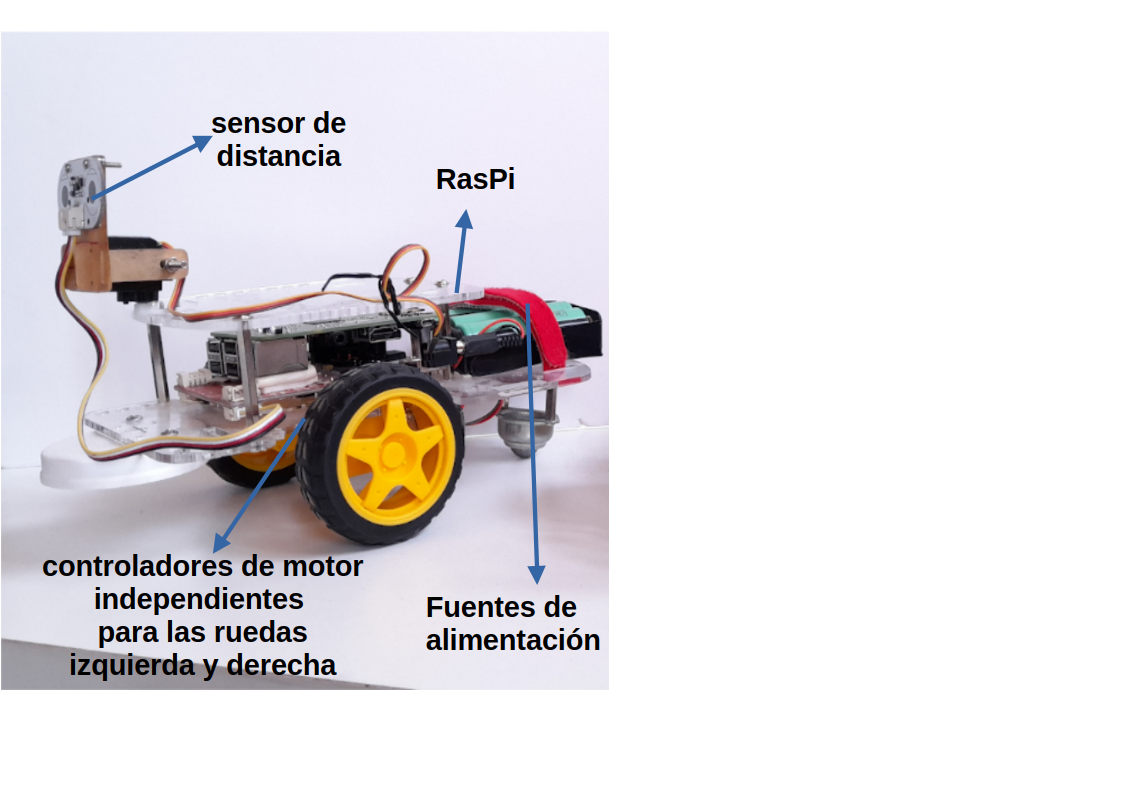
\includegraphics[width=\imsize]{robot_gopigo.png}
	\caption[Esquema del Robot GoPiGo de Dexter Industries, Mostrando Sensores de Distancia, Motores y Raspberry Pi Integrada, Utilizado en Conjunción con la Simulación del Connectoma de C. elegans.  ]{ Esquema del Robot GoPiGo de Dexter Industries, Mostrando Sensores de Distancia, Motores y Raspberry Pi Integrada, Utilizado en Conjunción con la Simulación del Connectoma de C. elegans.}\label{fig:robot}
\end{figure}



\subsection{Simulación de la dinámica neuronal en el connectoma de C. elegans}\label{sec:dinamica}

El robot sigue el diseño propuesto por Busbice, utilizando el connectoma de C. elegans (disponible en \url{https://github.com/openworm/}) para controlar un robot de dos ruedas. Para interactuar con el robot, se han creado dos módulos de Python: un módulo de entrada que lee los sensores del robot y estimula las neuronas apropiadas cuando se alcanzan umbrales específicos, y un módulo de salida que acumula estímulos de las neuronas motoras y, a su vez, envía la cantidad de potencia que se aplicará a cada uno de los dos motores. Estos dos módulos actúan como interfaces entre el robot y el connectoma.


\subsubsection{Modulo de entrada sensorial}

El robot utiliza un sensor de distancia GoPiGo para detectar obstáculos (\url{https://www.dexterindustries.com/store/distance-sensor/}). El sensor de distancia se ubica en la parte frontal del robot y se emplea para medir la distancia a los objetos en el camino del robot. Inicialmente, se utilizó un sensor ultrasónico estándar HC-SR04 para detectar obstáculos, pero se encontraron imprecisiones en las lecturas cuando el robot estaba en movimiento debido a que este tipo de sensor utiliza ondas de sonido para medir la distancia, y estas ondas pueden ser afectadas por el movimiento del robot. Por esta razón, se optó por cambiar al sensor GoPiGo Laser, el cual emplea el método de tiempo de vuelo para medir la distancia. Este método resulta mucho más preciso y no se ve afectado por el movimiento del robot. El proceso de detección de obstáculos funciona de la siguiente manera:


\begin{enumerate}
\item El sensor de distancia emite un pulso láser.
\item El pulso láser rebota en el obstáculo y regresa al sensor de distancia.
\item El sensor de distancia mide el tiempo que tarda el pulso láser en viajar de ida y vuelta.
\item Utilizando el tiempo de viaje, el sensor de distancia calcula la distancia al obstáculo.
\end{enumerate}


El sensor GoPiGo Laser ofrece varias ventajas sobre otros sensores de distancia basados en ultrasonido, incluyendo su precisión, velocidad y alcance. Puede medir la distancia de manera rápida y precisa, lo que lo convierte en una elección idónea para aplicaciones que requieren detección de obstáculos en tiempo real y con un alcance de hasta 5 metros, lo que resulta adecuado para situaciones en las que se necesita detectar obstáculos a distancia. Además de estas ventajas, el sensor GoPiGo Laser es fácil de instalar y usar, ya que se puede conectar a un puerto I2C en la placa Raspberry Pi y se puede utilizar con la biblioteca \textbf{DistanceSensor}. Las instrucciones detalladas sobre cómo conectar el sensor de distancia al robot se encuentran disponibles en \url{https://www.dexterindustries.com/GoPiGo/get-started-with-the-gopigo3-raspberry-pi-robot/}.


Basándonos en resultados de experimentos neurobiológicos y etológicos que demuestran que la nariz de C. elegans es una región altamente sensible, lo que lleva al nematodo a detenerse y cambiar de dirección cuando se encuentra con obstáculos (\Cref{sec:toquenariz}), decidimos utilizar el sensor mencionado para simular el sentido del tacto en la nariz del gusano. El sensor se activa cuando el robot se encuentra a menos de 30 centímetros de un objeto, una distancia que se ha comprobado ser efectiva. Las neuronas sensoriales estimuladas cuando el robot se encuentra a menos de 30 cm de un objeto son las siguientes: ASHL, ASHR, FLPL, FLPR, OLQDL, OLQDR, OLQVL, OLQVR, todas asociadas a este circuito sensorial.


\subsubsection{Detección de comida}

Detección de comida: Cuando el sensor de distancia no detecta obstáculos, estimulamos las neuronas quimiosensoriales responsables de la búsqueda de alimentos. Basándonos en resultados experimentales (\Cref{sec:quimiosensacion}) del comportamiento de búsqueda de alimentos, estimulamos las siguientes neuronas: ADFL, ADFR, ASGL, ASGR, ASIL, ASIR, ASJL, ASJR. En general, la estimulación de las neuronas sensoriales de alimentos activa el connectoma de manera más efectiva y hace que el robot comience a moverse hacia adelante.


 \subsubsection{Modulo de salida motora}
 
 
 Módulo de salida motora: El módulo de salida motora captura las salidas de las neuronas motoras y almacena los valores en una matriz en la que cada celda representa un músculo del cuerpo de C. elegans. Las neuronas motoras se conectan a los músculos para excitarlos o inhibirlos. El circuito neuromotor del gusano utiliza conexiones excitatorias e inhibidoras, lo que permite al gusano moverse de manera ondulante, contrayendo algunos músculos mientras relaja otros y viceversa. En total, hay 95 músculos corporales que recorren todo el cuerpo del gusano: 24 en la parte superior izquierda, 23 en la parte inferior izquierda, 24 en la parte superior derecha y 24 en la parte inferior derecha. Los músculos del cuerpo se dividen en izquierdos y derechos, y el valor acumulado se envía a los motores respectivos del robot. La velocidad máxima del motor se establece en 1000 DPS (grados por segundo), aunque este valor se suele reducir a 150 para evitar movimientos excesivamente rápidos en superficies lisas, aunque puede ajustarse en cualquier momento. Cuando el valor acumulado excede 150, el programa de salida lo restablece a 150. La relación entre los valores acumulados de los músculos izquierdos y derechos determina las señales que se envían a los motores del robot. La \Cref{fig:robot_2} muestra un diagrama de flujo que representa cómo se genera la salida motora.
 

 
  \begin{figure}[h!]
 	\centering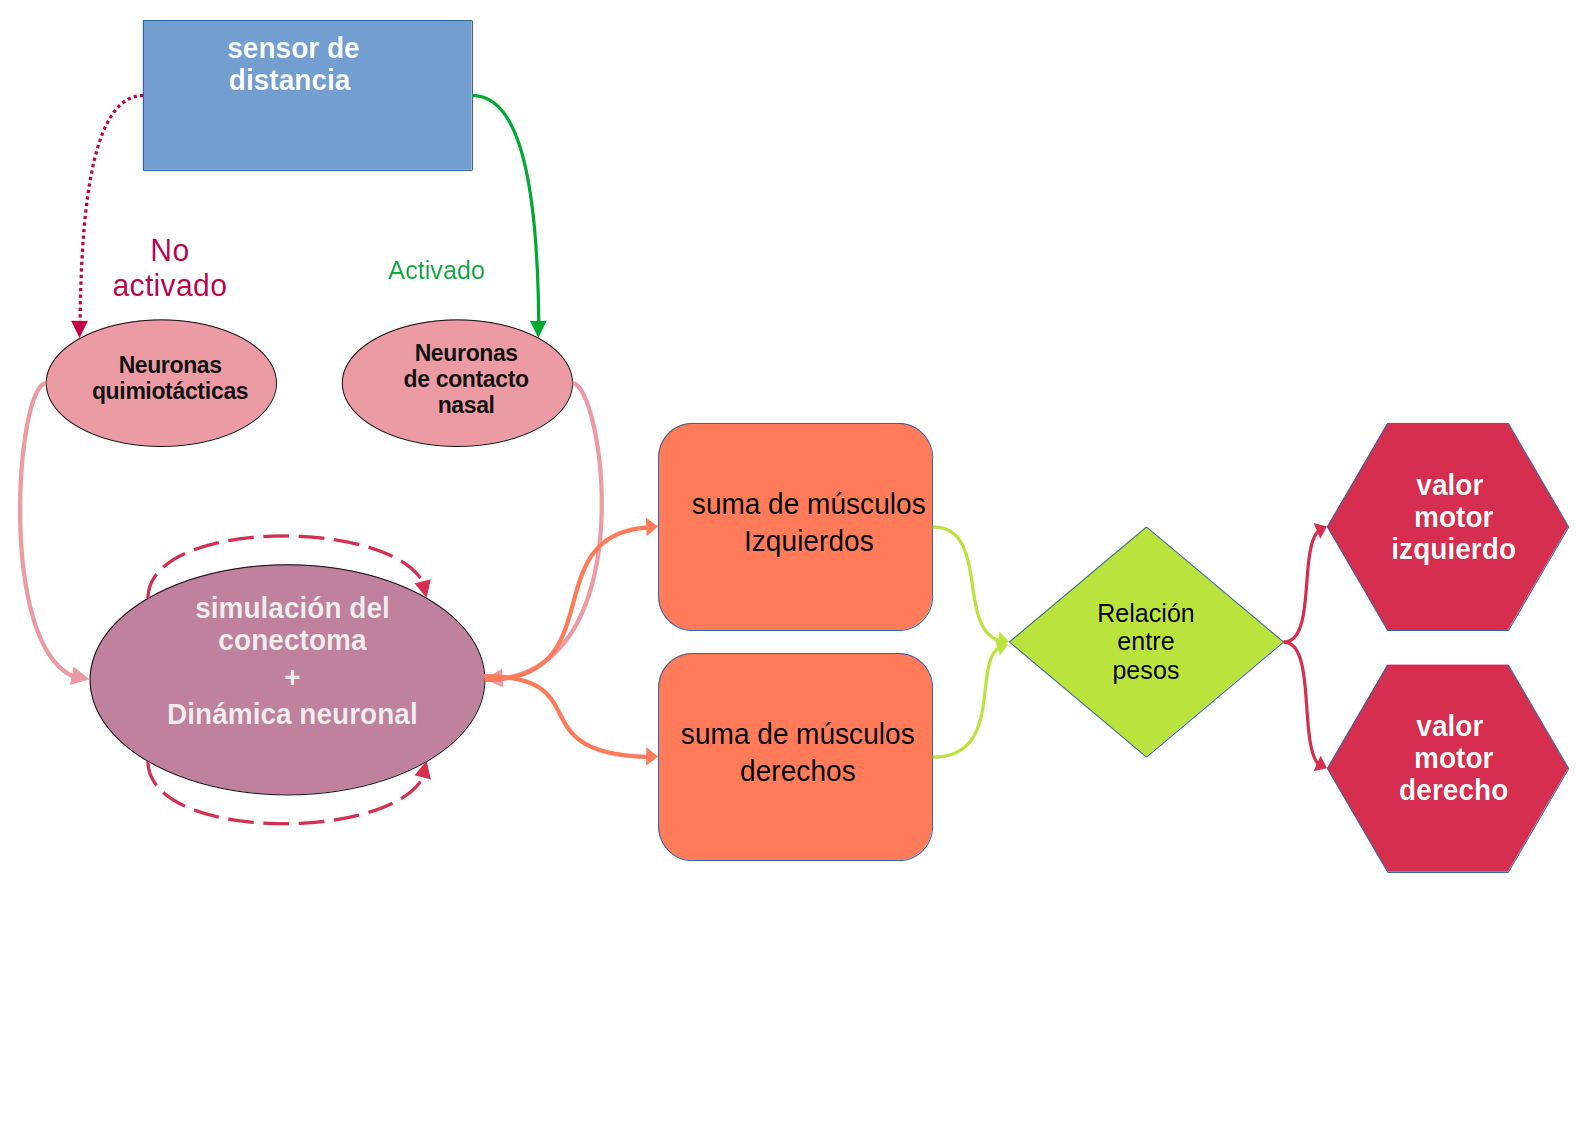
\includegraphics[width=\imsize]{robot_2.png}
 	\caption[Diagrama de Flujo que Ilustra la Generación de la Salida Motora.]{Diagrama de Flujo que Ilustra la Generación de la Salida Motora.}\label{fig:robot_2}
 \end{figure}
 

 
 
  \subsubsection{Modulo del conectoma}
 
El connectoma en sí se compone de un diccionario de Python con 300 entradas, cada una representando una neurona del connectoma de C. elegans (por ejemplo, AVAL, DB02 y VD03). Cada neurona está asociada a un diccionario que contiene las conexiones con otras neuronas, y el número de conexiones se utiliza como valor ponderado. Cuando una neurona dispara, se envía un valor ponderado a las neuronas conectadas. El programa principal se encarga de coordinar la simulación y controlar el robot.


 \subsection{Robot personalizado}

El robot personalizado sigue esencialmente los mismos pasos de construcción que el GoPiGo, pero en lugar de utilizar la placa GoPiGo 2 para el control de motores, emplea un controlador de motor dual L9110S (consulte las \Cref{fig:robot_personalizado,fig:robot_nuestro1,fig:robot_nuestro2}). En las \Cref{fig:sensor_distancia1,fig:sensor_distancia2} se muestra el diagrama de cableado del robot personalizado, que incluye la conexión del sensor de distancia directamente a la Raspberry Pi 3B y el cableado del controlador de motor L9110S.


\begin{figure}[h!]
	\centering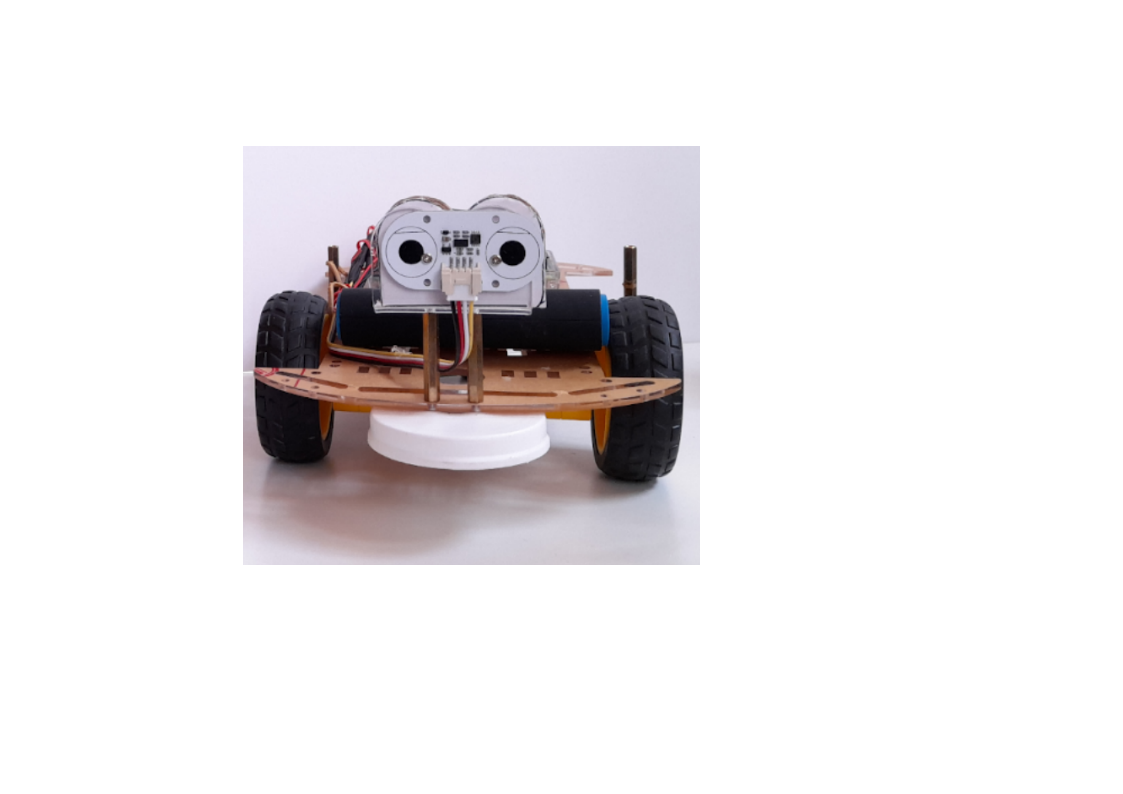
\includegraphics[width=\imsize]{robot_personalizado}
	\caption[Robot Personalizado Empleado en Nuestros Experimentos. ]{ Robot Personalizado Empleado en Nuestros Experimentos. Dado que el hardware del robot GoPiGo no es de código abierto, optamos por construir un robot personalizado, como se muestra a la derecha en la figura. En lugar de la placa GoPiGo 2, utilizamos un controlador de motor dual L9110S para el control de los motores. Este enfoque permite la construcción asequible del robot con componentes de fácil acceso y bajo costo.}\label{fig:robot_personalizado}
\end{figure}


\begin{figure}[h!]
	\centering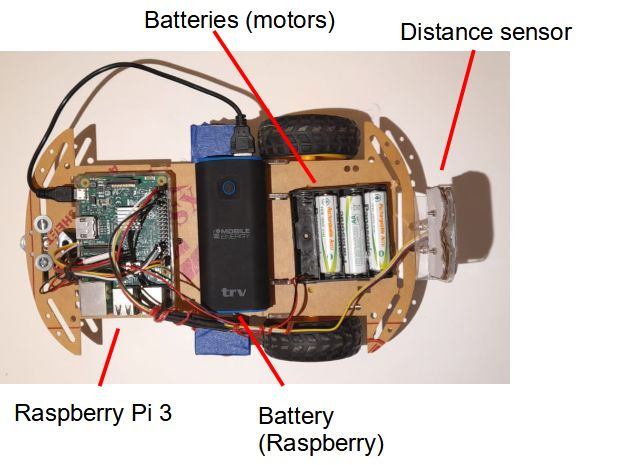
\includegraphics[width=\imsize]{robot_nuestro1.png}
	\caption[Vista Superior del Robot Personalizado.  ]{ Vista Superior del Robot Personalizado. En la imagen, se observa a la izquierda la Raspberry Pi, que ejecuta la simulación numérica para controlar el robot. La caja rectangular negra representa la batería que suministra energía a la Raspberry Pi, mientras que se emplea un paquete de baterías independiente para alimentar los motores. Además, se aprecia un sensor de distancia ubicado en la parte frontal del robot. }\label{fig:robot_nuestro1}
\end{figure}



\begin{figure}[h!]
	\centering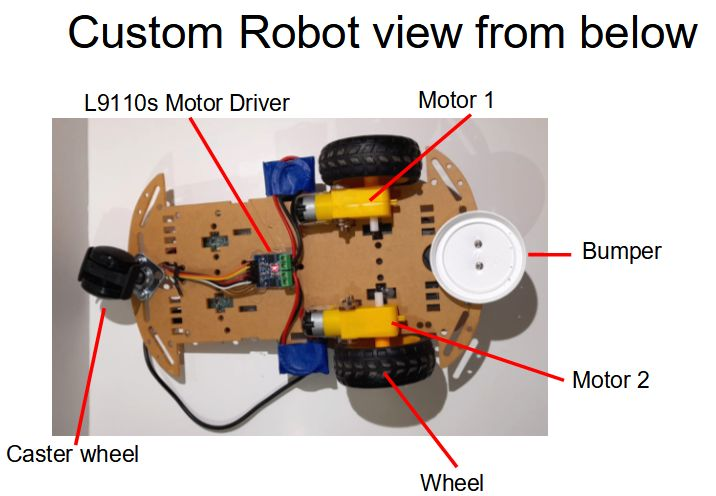
\includegraphics[width=\imsize]{robot_nuestro2.png}
	\caption[ Perspectiva Inferior del Robot Personalizado.]{ Perspectiva Inferior del Robot Personalizado. En esta vista, se aprecia la rueda giratoria a la izquierda, que proporciona soporte y facilita la maniobrabilidad del robot. En la parte inferior se encuentra el pequeño controlador de motores L9110s, permitiendo una conexión directa a los motores (en amarillo) que controlan las ruedas. Para proteger el sensor de distancia de posibles colisiones, se ha adjuntado un parachoques de goma en la parte delantera del vehículo.}\label{fig:robot_nuestro2}
\end{figure}


\begin{figure}[h!]
	\centering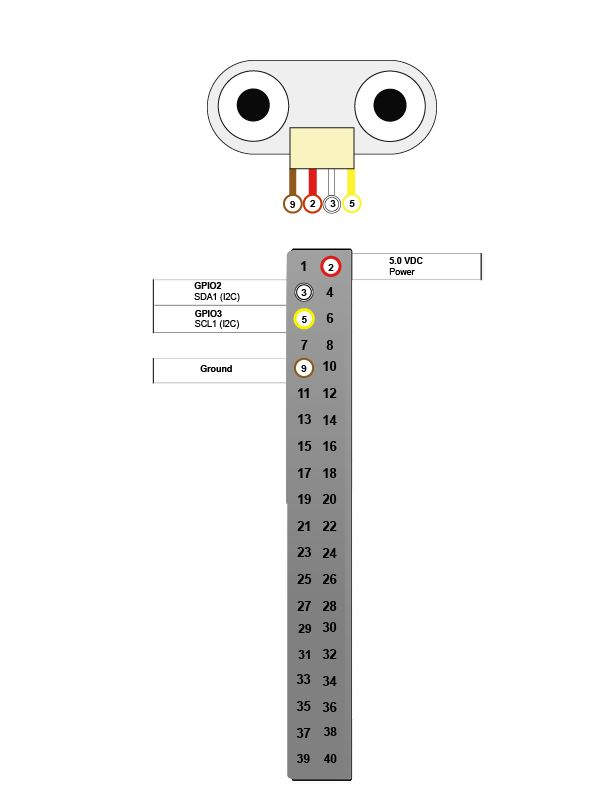
\includegraphics[width=\imsize]{sensor_distancia1.png}
	\caption[Conexión del Sensor de Distancia. ]{Conexión del Sensor de Distancia. En esta representación, se ilustra la conexión del sensor de distancia del GoPiGo directamente a los encabezados GPIO de una Raspberry Pi 3B en el robot personalizado. Las conexiones incluyen: Tierra (Ground), pin 9 (marrón), Alimentación (Power), pin 2 (rojo), SDA1 I2C, pin 3 (GPIO2, blanco) y SCL1 I2C, pin 5 (GPIO3, amarillo).}\label{fig:sensor_distancia1}
\end{figure}


\begin{figure}[h!]
	\centering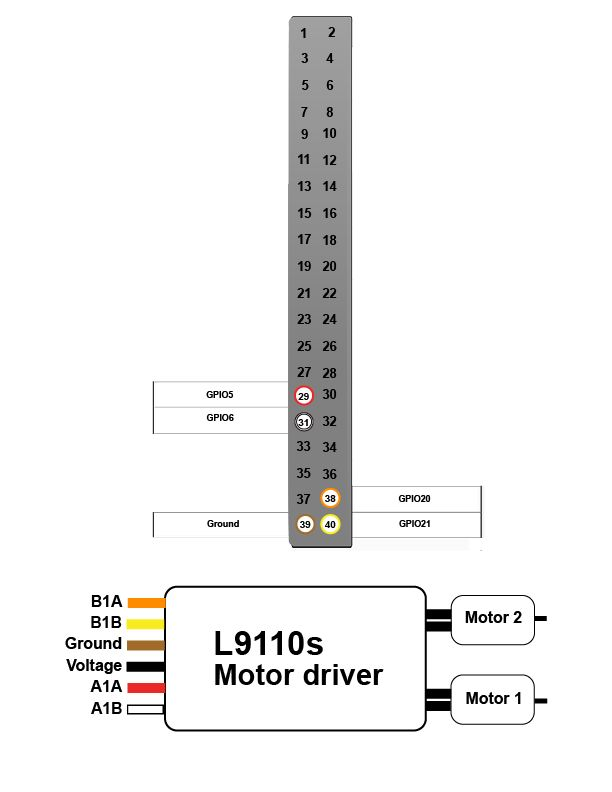
\includegraphics[width=\imsize]{sensor_distancia2.png}
	\caption[Conexión del Controlador de Motor.]{ Conexión del Controlador de Motor. En esta ilustración, se detalla cómo el controlador del motor L9110s se conecta a ambos motores y a los encabezados GPIO de una Raspberry Pi 3B en el robot personalizado. Las conexiones comprenden: B1A, pin 38 (GPIO20, naranja), B1B, pin 40 (GPIO21, amarillo), Tierra, pin 39 (marrón), Voltaje (conexión directa a la batería de 5V, negro), A1A, pin 29 (GPIO5, rojo) y A1B, pin 31 (GPIO6, blanco).}\label{fig:sensor_distancia2}
\end{figure}


\section{Dinámica neuronal global}\label{sec:dinamicakato}

Para explorar la dinámica global del robot que emula la actividad neuronal del C. elegans, hemos seguido la metodología propuesta por Kato et al. \cite{kato_global_2015}. En una primera etapa, calculamos las derivadas temporales de la actividad neuronal del robot. Para lograr esto, empleamos el método de diferenciación regularizada de variación total, cuyos detalles y justificaciones se encuentran en el \Cref{C:ap1}. La regularización desempeña un papel fundamental al reducir el ruido y la variabilidad en los datos, sin comprometer la información crítica.


Posteriormente, aplicamos el Análisis de Componentes Principales (PCA) a las derivadas temporales. Para este propósito, utilizamos la función de \textbf{PCA} de la biblioteca scikit-learn \footnote{https://scikit-learn.org/stable/modules/generated/sklearn.decomposition.PCA.html}. Esta técnica nos permitió no solo obtener los componentes principales (PC) ponderados de las neuronas, sino también calcular la varianza explicada por cada uno de estos componentes. Los PC se derivaron considerando la estructura de covarianza presente en los datos normalizados. Para una comprensión más completa de los PC, se recomienda la lectura de la referencia  \cite{noauthor_principal_2002}.

Con el objetivo de facilitar la interpretación de los resultados, aplicamos un filtro de promedio móvil a las trayectorias en el espacio de fases generadas mediante PCA. Este filtro consistió en un promedio de 10 muestras sucesivas. Paralelamente, generamos una serie de tiempo correspondiente a cada PC, denominada PC temporal. Esta serie se obtuvo mediante un promedio ponderado de las series temporales que abarcaban múltiples neuronas. Los PC temporales capturan señales compartidas por grupos de neuronas, que se agrupan en función de sus correlaciones.


Es importante destacar que realizamos el análisis PCA sobre las derivadas temporales de los datos, ya que los PC resultantes produjeron trayectorias en el espacio de estado que presentaban una organización espacial más coherente. Este enfoque nos brindó una visión más estructurada y representativa de la dinámica global del robot y su relación con el conectoma del C. elegans.



\section{Discusión}

En el marco de nuestra investigación, la elección de este diseño específico de robot se fundamenta en sus características intrínsecamente atractivas. La simplicidad en su construcción y su costo reducido lo destacan como una opción altamente replicable y económicamente eficiente en el contexto de la investigación científica. No obstante, la innovación reside en la simulación neuronal que rige el comportamiento del robot. Dicha simulación se basa en unidades dinámicas elementales e incorpora información biológica derivada del conectoma, lo que confiere al robot la capacidad de manifestar comportamientos emergentes, permitiéndole desenvolverse de manera autónoma y sortear obstáculos de forma natural.

Este modelo presenta una serie de distinciones clave en comparación con la mayoría de las simulaciones:

Primero, se trata de un modelo completo del conectoma, aunque es importante tener en cuenta que no se han incorporado todos los orgánulos o entradas sensoriales en el modelo en la etapa actual. Por ejemplo, los receptores de estiramiento, que podrían desempeñar un papel importante en los comportamientos de locomoción de C. elegans, aún no forman parte de este modelo en su estado actual de desarrollo.

Además, a diferencia de las simulaciones discretas, este modelo sigue una dinámica continua. La estimulación es constante y activa, imitando la operación de un sistema nervioso en tiempo real. Las modificaciones en la información sensorial tienen un impacto directo y continuo en el comportamiento del robot.

La naturaleza física del modelo también es una característica distintiva. El Connectome se encuentra conectado a un robot tridimensional real, lo que posibilita una interacción genuina con su entorno. Esta interacción es altamente impredecible y fundamental para la comprensión del comportamiento emergente.

En lo que respecta a la representación neuronal, cada neurona se modela mediante un programa individual, en analogía con el funcionamiento de las neuronas biológicas. Las entradas dendríticas y las salidas axonales solo responden a la cantidad de estimulación recibida por el programa correspondiente.

Dado que el Conectoma se representa mediante programas individuales, el tiempo de generación de la estimulación no es fijo, sino que varía según la evolución de los factores ambientales. El aspecto temporal es crucial, ya que la estimulación cambia a medida que los factores ambientales se modifican. Cada programa se configura para disparar su axón solo cuando se alcanzan ciertos umbrales, y con el tiempo, el programa se despolariza.

Sin embargo, a pesar de las ventajas mencionadas, hasta el momento no hemos realizado un análisis exhaustivo de la dinámica del modelo ni de su correlación con las acciones del robot. El capítulo siguiente se enfoca en presentar los resultados derivados de la aplicación de este modelo robótico al estudio del comportamiento motor emergente. Además, buscamos, en la medida de lo posible, comparar los resultados obtenidos en el robot con aquellos provenientes de experimentos recientes con C. elegans. Este enfoque nos brinda la oportunidad de adquirir una comprensión más profunda de la capacidad del modelo para simular con precisión el comportamiento del organismo biológico.












\chapter{Resultados de Comportamientos emergentes en Robots con el  Conectoma de C. elegans}\label{cap:resultados_robot}
\graphicspath{{figs/capitulo_resultados_robot/}}

\chapterquote{Far from being able to accept the idea of the individuality and independence of  	each nerve element, I have never had reason, up to now, to give up the concept 	which I have always stressed, that nerve cells, instead of working individually, act 	together [...]. However opposed it may seem to the popular tendency to individualize the elements, I cannot abandon the idea of a unitary action of the 	nervous system [...]}{Camillo Golgi, 1906}


El comportamiento adaptativo es un atributo distintivo de los organismos vivos y se manifiesta en su capacidad para responder con flexibilidad a las señales sensoriales. La comprensión de cómo los circuitos neuronales logran esta adaptabilidad es esencial para la neurociencia y la inteligencia artificial. En particular, es crucial descubrir cómo un conectoma anatómicamente estático puede ser modulado para permitir la regulación dinámica de la conectividad funcional en la red neuronal. En esta sección, mostraremos los resultados de  una investigación que se embarcó en el desafío de abordar esta cuestión fundamental.

La orientación en el entorno es una habilidad fundamental para un robot autónomo. En la naturaleza, los seres vivos, incluso los más simples, exhiben impresionantes capacidades de control de orientación. La supervivencia de muchas especies depende en gran medida de su capacidad para navegar en el espacio, lo que les permite buscar refugio, encontrar recursos alimenticios y emparejarse. Los mecanismos que permiten a los organismos detectar y responder a una amplia variedad de estímulos ambientales han evolucionado a lo largo del tiempo. Esta capacidad de orientación se ha convertido en un enigma intrigante y un punto de partida inspirador para el diseño de controladores de orientación de robots.

La importancia de comprender los mecanismos de control motor no puede subestimarse. Por lo tanto, en esta investigación, utilizamos un robot que incorpora el conectoma de C. elegans, un organismo modelo ampliamente estudiado en la biología. Nuestra elección se basa en la idea de que la eficacia de un robot en tareas de navegación y evitación de obstáculos podría arrojar luz sobre el funcionamiento de la habilidad motora de un organismo vivo. Para evaluar esta eficacia, diseñamos y ejecutamos una serie de experimentos en un entorno altamente controlado. Nuestro enfoque no se limita a un solo robot, sino que involucra tanto al robot comercial GoPiGo como a un robot de construcción personalizada. Esta elección meticulosa garantiza que los resultados sean consistentes y reproducibles en diferentes configuraciones y con diversas plataformas de robots.

El resultado de nuestros experimentos demostró la capacidad de los robots para detectar obstáculos y ajustar sus trayectorias, lo que a su vez les permitió navegar de manera segura en su entorno. Estos resultados son prometedores y abren la puerta a nuevas perspectivas para el diseño de robots autónomos y la comprensión de los principios subyacentes a la orientación en el espacio.

Este capítulo presenta los resultados de nuestra investigación y ofrece una visión más profunda de la relación entre el conectoma, la función y el comportamiento. Nuestros experimentos tienen como objetivo desentrañar cómo se ensamblan las dinámicas de la red neuronal y cómo la estructura del conectoma y las conexiones sinápticas dan lugar a los comportamientos observados. Además, buscamos identificar en la dinámica de los robots algunas características fundamentales que pueden compararse con la dinámica neuronal global de C. elegans. Al explorar la presencia de grupos de neuronas sincronizadas y una estructura jerárquica anidada, buscamos establecer vínculos entre la compleja estructura de red del connectoma y las características emergentes en la dinámica del robot.

Estos resultados no solo tienen implicaciones para la comprensión de cómo los organismos vivos se adaptan y responden a entornos cambiantes, sino que también abren nuevas vías de investigación en el campo de la inteligencia artificial. Al dotar a sistemas cibernéticos con características complejas inspiradas en seres vivos, podríamos avanzar hacia una nueva generación de inteligencia artificial que se base en principios biológicos. Además, la capacidad de realizar experimentos controlados con un organismo cibernético nos permitirá probar hipótesis de manera precisa y avanzar en nuestra comprensión de la adaptación biológica.

Esta sección de resultados es un paso importante hacia la confluencia de la biología y la robótica, y esperamos que los hallazgos presentados aquí inspiren investigaciones futuras en campos interdisciplinarios y abran nuevas perspectivas sobre la adaptación y la inteligencia.

 
\section{Evaluación del Comportamiento del Neurorobot}

Antes de llevar a cabo cualquier medición o análisis de la dinámica neuronal simulada del C. elegans, así como del comportamiento emergente del neurorobot en el que se implementa, es esencial garantizar la robustez y la idoneidad de los parámetros que controlan la dinámica neuronal del modelo. Además, se debe asegurar que el comportamiento resultante sea coherente con lo observado en organismos reales. En esta sección, se llevaron a cabo un conjunto de pruebas para verificar el óptimo funcionamiento de los algoritmos que simulan la dinámica neuronal del C. elegans y el comportamiento que emerge del robot.

\subsection{Prueba del Parámetro de Umbral ($h$)}	

La dinámica microscópica de nuestro modelo neurorobótico, expresada en la ecuación 1, se encuentra bajo la influencia de un parámetro de control denominado $h$. Con el fin de examinar cómo varía el comportamiento emergente en función de este parámetro, se llevaron a cabo experimentos de cinco minutos en varios rangos de valores de $h$. Posteriormente, se analizaron tanto el comportamiento macroscópico del robot como las matrices de dinámica neuronal y de acciones registradas. Los resultados se presentan en las \Cref{fig:valores_neuronas_umbrales,fig:accion_umbrales} .


\begin{figure}[h!]
	\centering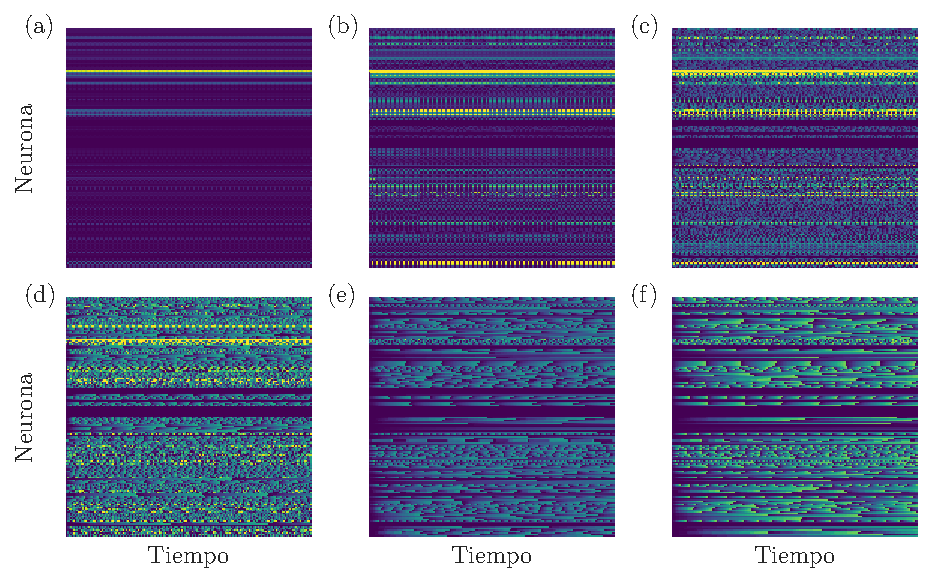
\includegraphics[width=\imsize]{valores-neuronas_umbrales.pdf}
	\caption[ Resultados de la Prueba del Parámetro de Umbral ($h$).]{ Las subfiguras (a-b) muestran la actividad de las neuronas cuando el umbral $h$ es demasiado bajo, lo que conduce a un comportamiento tipo epileptoide. En las subfiguras (c-d), se observa que la actividad neuronal se apaga cuando el umbral es demasiado alto, resultando en un estado comatoso del robot. Finalmente, en las subfiguras (e-f), se muestra la actividad óptima con un umbral intermedio, similar a los experimentos con organismos reales. }\label{fig:valores_neuronas_umbrales}
\end{figure}


\begin{figure}[h!]
	\centering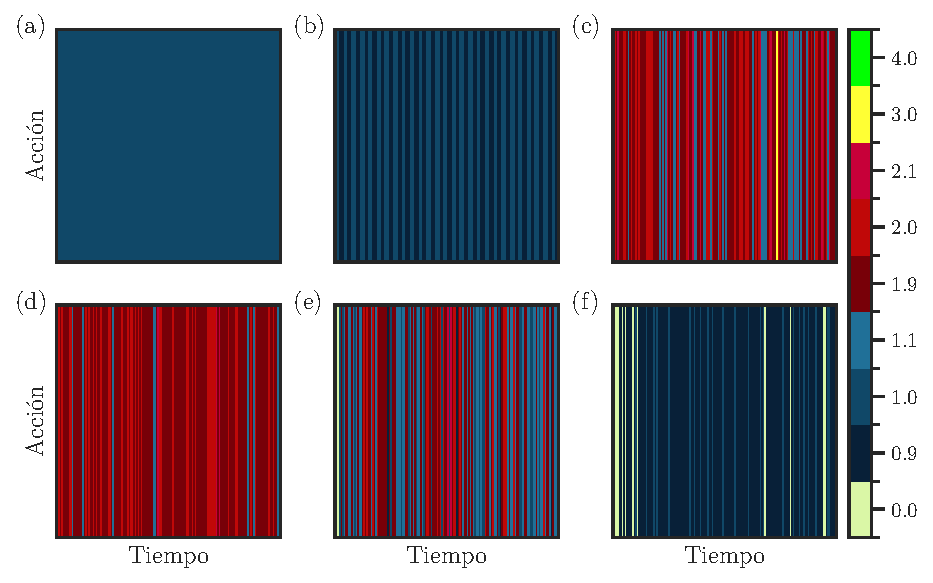
\includegraphics[width=\imsize]{accion_umbrales.pdf}
	\caption[ Matrices de Acciones Correspondientes a la Prueba de Umbral ($h$).]{ Matrices de Acciones Correspondientes a la Prueba de Umbral ($h$). Las subfiguras (a-b) muestran las acciones del robot cuando el umbral $h$ es demasiado bajo, lo que resulta en un comportamiento caótico. En las subfiguras (c-d), se observa la ausencia de movimiento cuando el umbral es demasiado alto. Por último, en las subfiguras (e-f), se representan las acciones complejas y coherentes con un comportamiento emergente óptimo, como el retroceso al encontrar obstáculos, cuando se utiliza un umbral intermedio. }\label{fig:accion_umbrales}
\end{figure}





Cuando el umbral $h$ es demasiado bajo (por ejemplo, $h=1$ o $h=5$), la mayoría de las neuronas disparan en cada paso de tiempo (\Cref{fig:valores_neuronas_umbrales}a-b). Este fenómeno resulta en la ausencia de una actividad de red rica y coordinada, es decir, no se observan grupos de neuronas sincronizadas. Como consecuencia, el comportamiento del robot se asemeja a un estado epiléptico, con giros en múltiples direcciones y avance constante, como se refleja en la matriz de acciones registrada (\Cref{fig:accion_umbrales}a-b). En estos valores, no se manifiestan comportamientos emergentes significativos.

Por otro lado, cuando el umbral es demasiado alto ($h>100$), casi ninguna neurona dispara, ya que se requieren numerosos pasos de tiempo para que las neuronas alcancen el umbral. En este escenario, la actividad de la red neuronal se encuentra apagada (\Cref{fig:valores_neuronas_umbrales}c-d), con un número reducido de neuronas sincronizadas. Esto conduce a un comportamiento que se asemeja a un estado comatoso del robot, donde prácticamente no se observa movimiento (\Cref{fig:accion_umbrales}c-d).

Finalmente, se observa que solo en los rangos intermedios (por ejemplo, $h=15$ y $h=30$), la actividad de la red muestra grupos de neuronas sincronizadas (\Cref{fig:valores_neuronas_umbrales}e-f), similar a lo que se observa en experimentos con organismos reales. Las matrices de acciones (\Cref{fig:accion_umbrales}e-f) concuerdan con un comportamiento emergente que implica acciones complejas, como la capacidad de retroceder al encontrar un obstáculo. Por lo tanto, se concluye que el comportamiento emergente del robot es óptimo en los rangos intermedios del umbral. Es importante destacar que, no obstante, este valor no requiere un ajuste preciso, ya que se obtuvieron resultados cualitativamente similares para umbrales que oscilan entre 10 y 100. Basándonos en estos resultados, se optó por el valor de umbral de 30 para el resto de los experimentos.

\subsubsection{Discusión}

Los hallazgos anteriores sugieren un comportamiento crítico, similar a lo que se observa en la física estadística de las transiciones de fase. En este contexto, los comportamientos más complejos se manifiestan únicamente en una región de este diagrama, que se denomina \textquote{región crítica}. Estos resultados sugieren que el sistema nervioso de los organismos podría manifestar su óptimo funcionamiento dentro de un rango crítico. Motivados por estos hallazgos, en la segunda parte de esta tesis se profundiza en la hipótesis anteriormente mencionada, conocida en la literatura como la \textquote{hipótesis de criticidad neuronal}.

\subsection{Variación de las Pausas y su Impacto en el Comportamiento}

La observación del comportamiento emergente en el neurorobot plantea una interrogante fundamental: ¿Cómo es posible que una red neuronal, adaptada para controlar la locomoción de un gusano de apenas 1 mm de longitud, pueda aplicarse de manera efectiva en el control de un vehículo robótico de aproximadamente 30 cm de longitud? Esta sección muestra los resultados de investigar en profundidad cómo la incorporación estratégica de pausas en el programa de control, con una variación de duraciones que oscila entre 0.5 y 0.8 segundos, permite al robot ejecutar con precisión los comandos transmitidos por el conectoma. Este enfoque se traduce en una sincronización exitosa entre la escala temporal de las simulaciones y la escala de respuesta del vehículo robótico, lo que plantea la posibilidad de aplicar el conectoma del C. elegans para controlar robots de distintos tamaños. Esta sección se centra en el análisis de cómo la variación de las pausas afecta el comportamiento del robot.

Para alcanzar este objetivo, se llevaron a cabo experimentos de un minuto de duración, en los cuales se empleó el neurorobot para simular la dinámica neuronal del C. elegans con diferentes valores de pausas entre la emisión de comandos y la ejecución de acciones. El análisis se centró en la relación entre los comandos enviados al robot y las acciones efectivamente realizadas. Se encontró la  existencia de un amplio rango de duraciones de pausas en el que el robot exhibe un comportamiento similar. Sin embargo, se observa que cuando las pausas son notoriamente cortas, el robot no puede seguir las acciones con la suficiente velocidad, lo que da lugar a un comportamiento errático que, en última instancia, paraliza el movimiento del robot. El análisis de las matrices de acciones revela que muchas de las acciones programadas superan las limitaciones de velocidad del robot, lo que resulta en la no ejecución de más de la mitad de las acciones planificadas. Por otro lado, cuando las pausas son significativamente prolongadas, el robot experimenta considerables retrasos en la ejecución de acciones. En estas condiciones, las matrices de acciones exhiben intervalos extensos entre las acciones, semejantes a las de un organismo con un metabolismo considerablemente lento. Solo en valores intermedios de la duración de las pausas se consigue un comportamiento adecuado que permite la ejecución de acciones sin que se superpongan.

Las \Cref{fig:pause_bajo,fig:pause_alto} presentan una representación gráfica de las matrices de acciones correspondientes a pausas de duración corta y larga, respectivamente. En la Figura 1, se observa una alta densidad de acciones programadas en un espacio de tiempo breve, lo que sobrecarga al robot y produce un comportamiento caótico. Por otro lado, en la Figura 2, la escasa densidad de acciones indica una larga duración entre cada acción



\begin{figure}[h!]
	\centering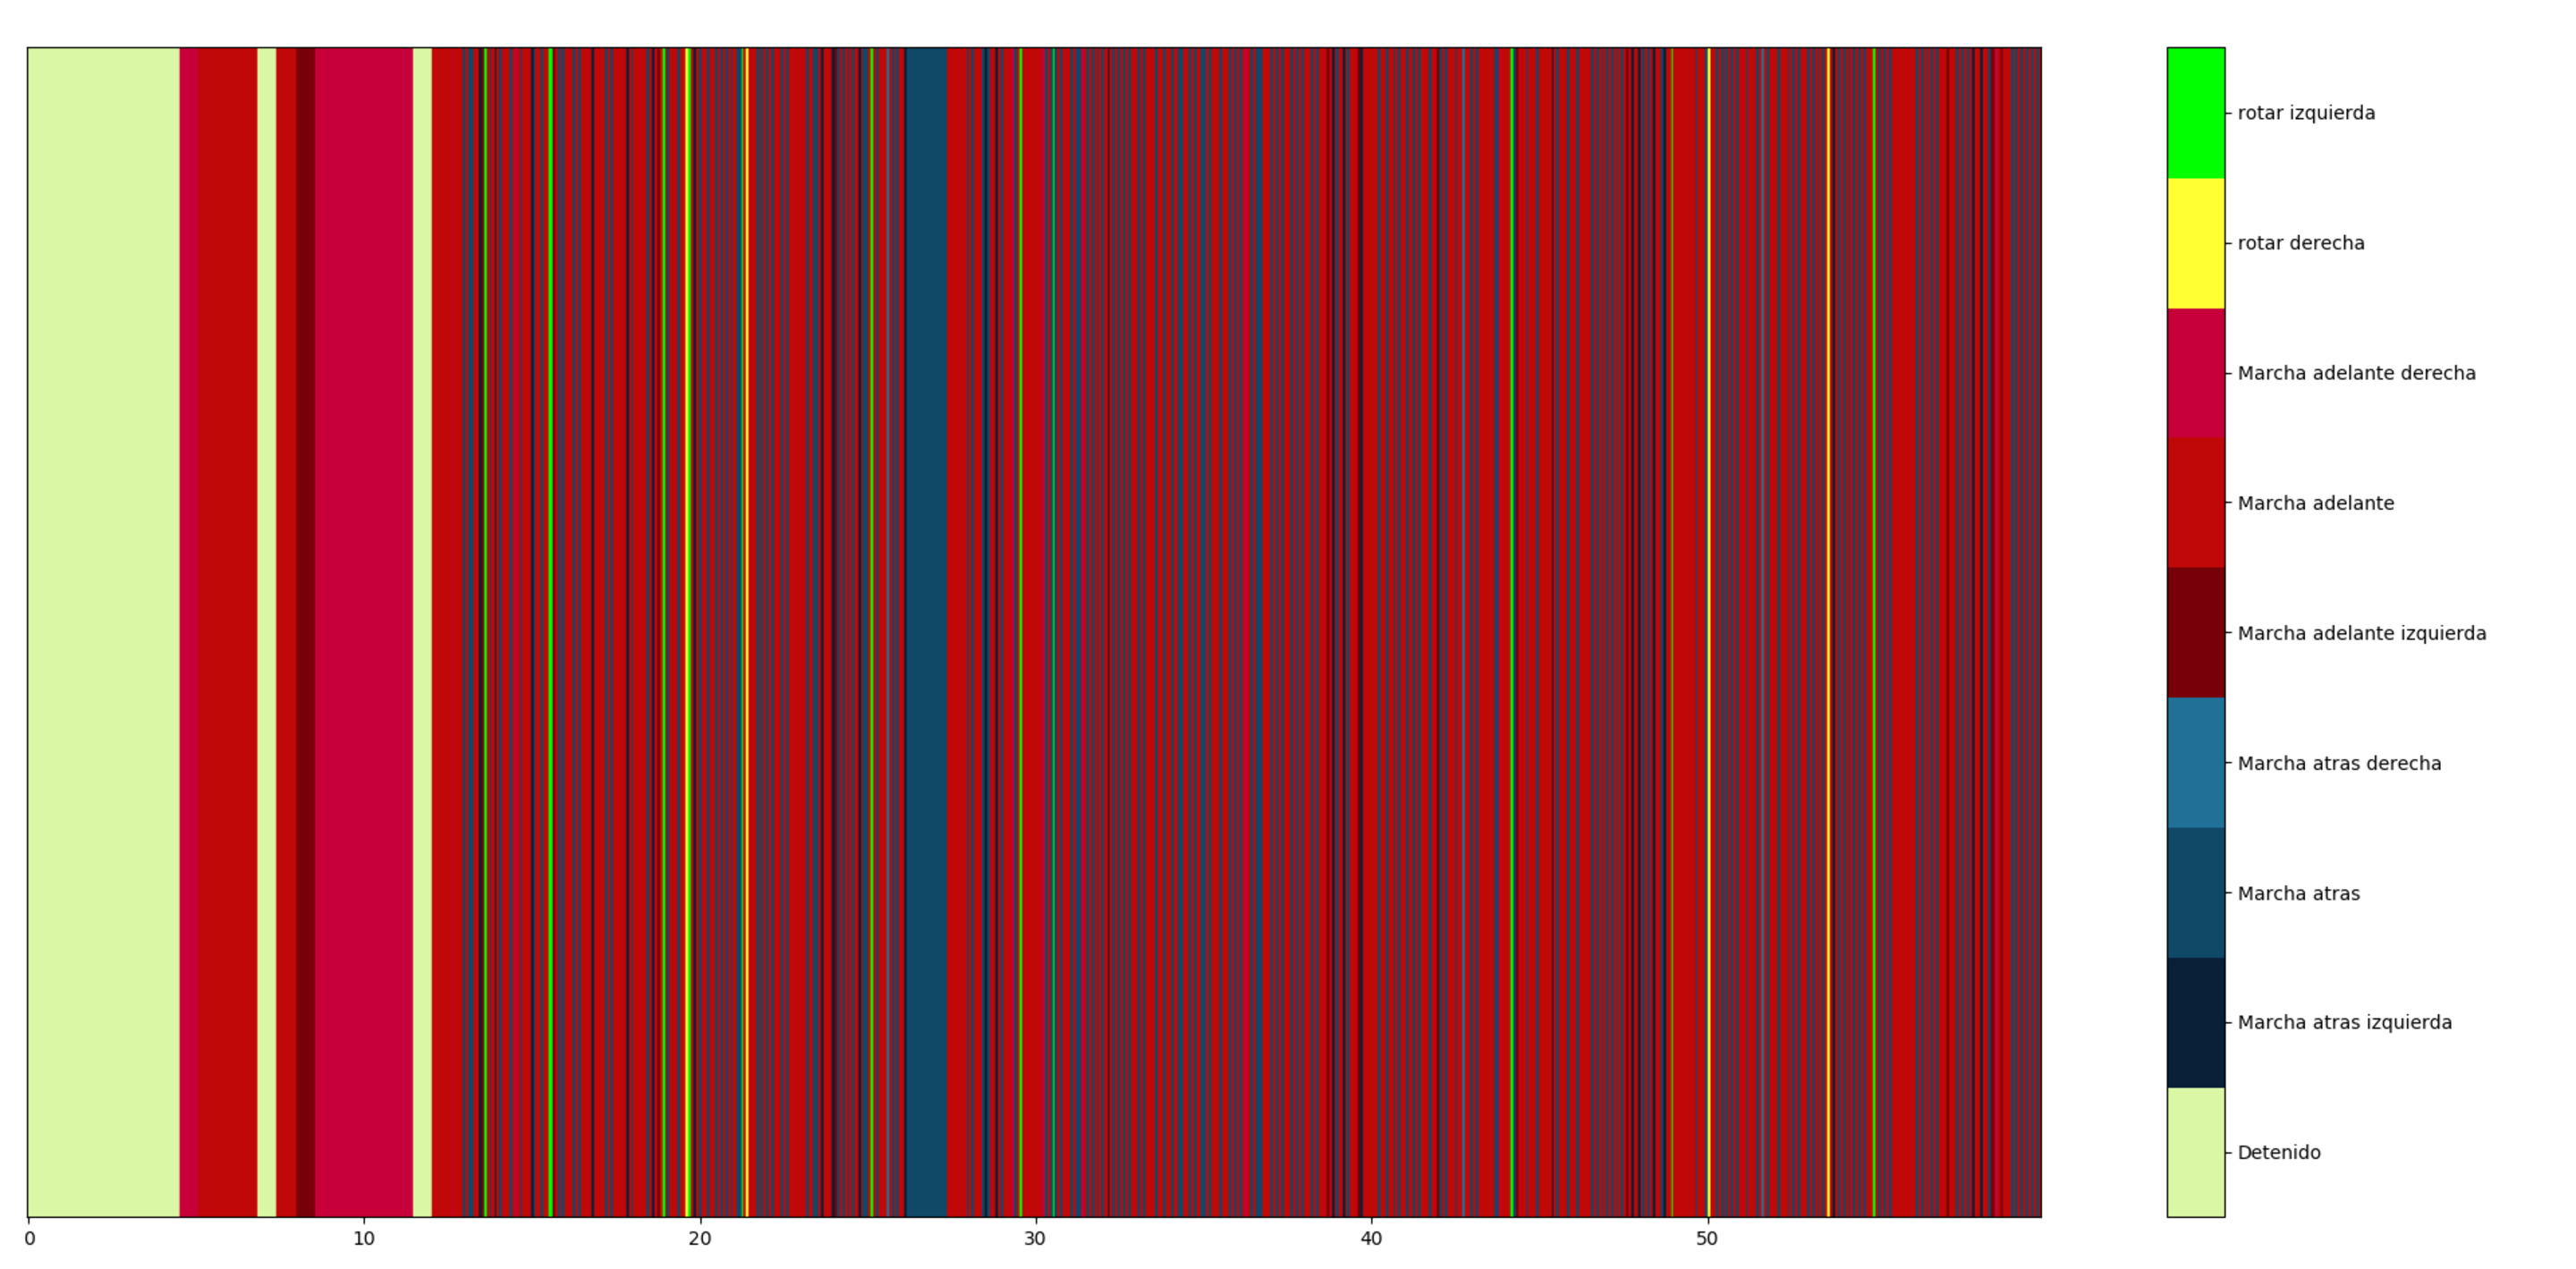
\includegraphics[width=\imsize]{pause_bajo.pdf}
	\caption[ Matriz de Acciones con Pausas largas.]{ Matriz de Acciones con Pausas largas. Esta figura presenta una matriz de acciones generada durante experimentos con pausas largas en el programa de control del robot, lo que da como resultado una baja densidad de acciones y un comportamiento más lento y deliberado, similar al de un organismo con un metabolismo lento.}\label{fig:pause_bajo}
\end{figure}


\begin{figure}[h!]
	\centering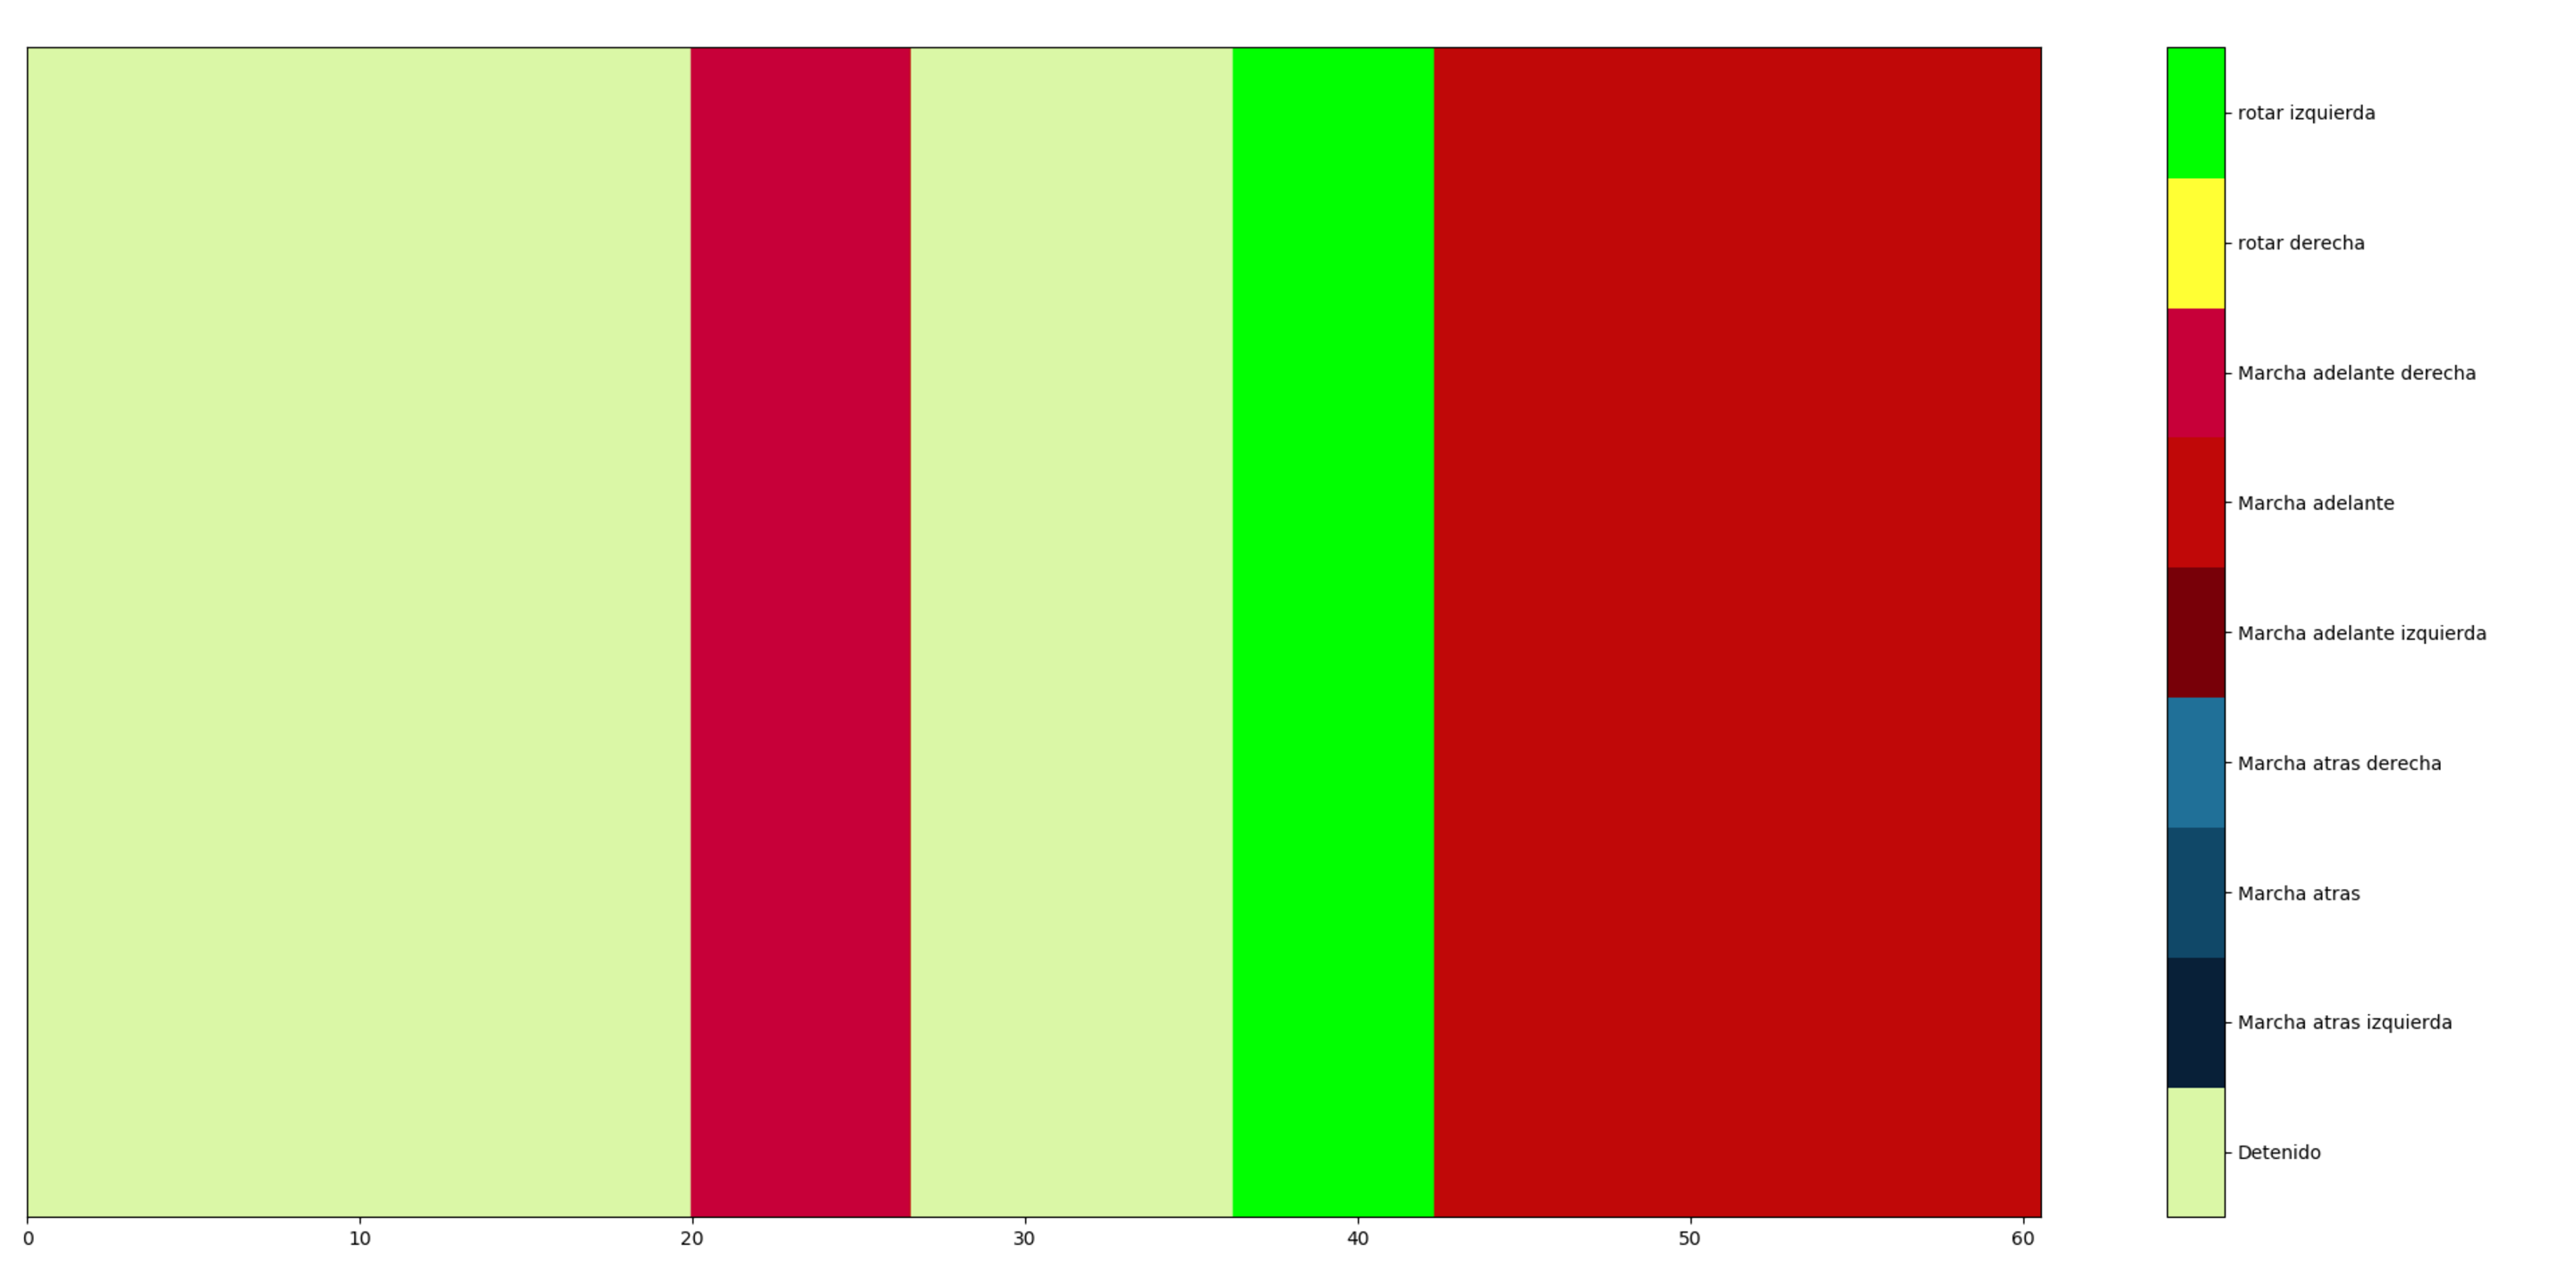
\includegraphics[width=\imsize]{pause_alto.pdf}
	\caption[ Matriz de Acciones con Pausas Cortas.]{ Matriz de Acciones con Pausas Cortas. Esta figura ilustra una matriz de acciones generada durante experimentos con pausas cortas en el programa de control del robot, lo que resulta en una alta densidad de acciones en un período de tiempo limitado, lo que provoca un comportamiento errático y sobrecarga en el robot. }\label{fig:pause_alto}
\end{figure}

\subsubsection{Discusión }

Los resultados anteriormente descritos evocan discusiones previas sobre el factor $h$ y los fenómenos tipo críticos. Se ha comprobado que la diferencia de tiempo entre la generación de un impulso neuronal (spike) y la ejecución de la acción juega un papel crucial en la manifestación de comportamientos complejos. En este sentido, las pausas en el programa de control pueden considerarse una simulación de aspectos neurales, como las dimensiones de los axones y las velocidades de propagación. Además, las pausas imitan la transición entre la generación de señales eléctricas y la traducción en acciones físicas.

Uno de los aspectos más notables de este resultado es la confirmación de que la sincronización precisa entre la generación de comandos y la ejecución de acciones es esencial para un control efectivo de los robots. Las pausas en el programa de control actúan como un amortiguador temporal que permite que las señales neurales se traduzcan en movimientos físicos de manera coherente. Este hallazgo es particularmente relevante para la robótica, donde la adaptabilidad y la eficiencia son fundamentales. Además, estos resultados sugieren que los robots controlados por redes neuronales pueden adaptarse a una variedad de tamaños y escalas, lo que tiene aplicaciones potenciales en el diseño de robots flexibles y versátiles.

En el futuro, se podría llevar a cabo una ampliación más detallada del modelo, incorporando elementos más biofísicos que representen con mayor precisión la diferencia entre un spike (impulso neuronal) y la ejecución de la acción. Esto no se limitaría a una simple pausa en el programa, sino que podría involucrar aspectos más complejos de la biología neuronal. De esta manera, el modelo podría adquirir una mayor organicidad y reflejar con mayor fidelidad los procesos observados en organismos reales. Estas investigaciones adicionales podrían contribuir de manera significativa al entendimiento de la relación entre la actividad neuronal y el comportamiento en sistemas biológicos y robóticos.




\subsection{Efectos de la Aleatoriedad en el Conectoma}\label{sec:aleaotrioconectoma}

Con el objetivo de evaluar si la aparición de grupos sincronizados es un fenómeno genuino y no un epifenómeno, llevamos a cabo un análisis de la dinámica neuronal en versiones aleatorizadas del conectoma del gusano C. elegans. Estas redes aleatorias conservan tanto la distribución de grados como la de pesos, es decir, mantienen el mismo grado de entrada y salida para las neuronas, con las conexiones y pesos distribuidos al azar \cite{milo_network_2002}.Esta sección del estudio tiene como propósito respaldar o refutar la hipótesis de que la complejidad de la red es fundamental para la emergencia del comportamiento, en contraste con una red completamente aleatoria.


Se realizaron un total de 10 experimentos, cada uno con una duración de 5 minutos, utilizando un conectoma aleatorio diferente. El robot fue ubicado en una caja de 1 metro de lado, lo que garantizó la reproducibilidad del experimento y el control de las variables. Además, se llevaron a cabo experimentos utilizando el conectoma no aleatorizado con el fin de realizar comparaciones. En todos los casos con conectomas aleatorizados, el robot no mostró comportamientos complejos emergentes, como se puede observar en el video suplementario 2 (\url{https://www.frontiersin.org/articles/10.3389/fnbot.2022.1041410/full#supplementary-material}). En todos estos experimentos, el robot exhibió patrones de comportamiento consistentes en giros repetitivos, avance sin retroceso y colisiones sin una respuesta coordinada. Esta falta de coherencia y coordinación en los comportamientos se refleja en la matriz de acciones (\Cref{fig:comportamiento_aleatorio}), donde se evidencia que el comportamiento complejo es prácticamente inexistente. En su mayoría, el robot permanece inmóvil o se desplaza hacia adelante o hacia atrás. La \Cref{fig:comportamiento_aleatorioneurona}, que muestra la dinámica neuronal, confirma la ausencia de grupos de neuronas sincronizadas que normalmente se esperaría encontrar en un organismo tan complejo como el C. elegans. Esta falta de comportamientos emergentes y sincronizados se observó en los 10 experimentos, lo que sugiere que la aleatoriedad no da lugar a comportamientos complejos, y que, por tanto, es la topología del conectoma la que permite la emergencia de comportamientos complejos.

\begin{figure}[h!]
	\centering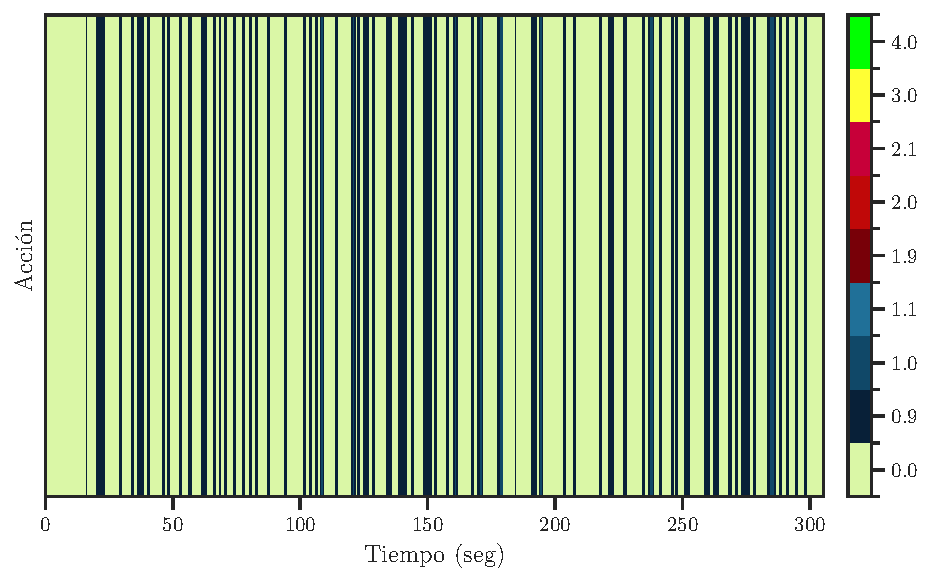
\includegraphics[width=\imsize]{accion_aleatorio.pdf}
	\caption[ Matriz de Acciones de un Conectoma Aleatorio.]{ Matriz de Acciones de un Conectoma Aleatorio. La Figura  muestra la matriz de acciones resultante de experimentos con un conectoma aleatorio. Los patrones de comportamiento del robot en este contexto carecen de coherencia y complejidad, predominando movimientos repetitivos sin respuestas coordinadas.  }\label{fig:comportamiento_aleatorio}
\end{figure}


\begin{figure}[h!]
	\centering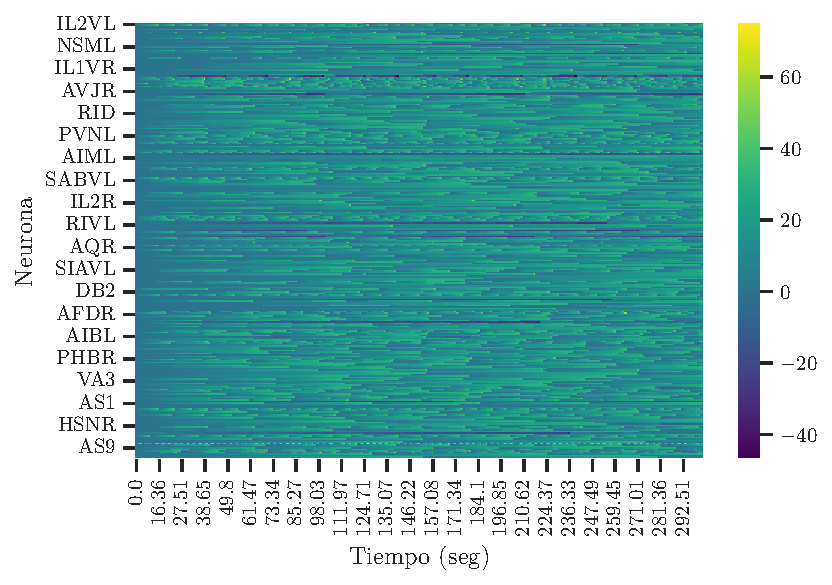
\includegraphics[width=\imsize]{matriz_valores_aleatorio.pdf}
	\caption[ Dinámica Neuronal en un Conectoma Aleatorio.]{ Dinámica Neuronal en un Conectoma Aleatorio.  En la Figura, se presenta la dinámica neuronal correspondiente a un conectoma aleatorio. Observamos la falta de grupos de neuronas sincronizadas, en contraste con lo que se esperaría encontrar en un organismo complejo como el C. elegans. }\label{fig:comportamiento_aleatorioneurona}
\end{figure}



En contraste, cuando el robot opera con la dinámica neuronal que contiene el conectoma del C. elegans, exhibe un comportamiento rico y complejo. Por ejemplo, cuando se enfrenta a un obstáculo, retrocede, emulando así el comportamiento del gusano real (véase la \Cref{fig:acciones} de la matriz de acciones en un experimento de 20 minutos). Además, en la dinámica neuronal se observan grupos de neuronas sincronizadas, tal como se muestra en la Figura 4, los cuales son comparables a los encontrados en experimentos con el C. elegans real (véase la \Cref{fig:kato} de un experimento con C. elegans realizado por Kato et al. \cite{kato_global_2015}).


\subsubsection{Discusión}

Los resultados previos son de relevancia, ya que si el comportamiento del robot con un conectoma aleatorio fuera idéntico al observado con el conectoma real, se podría argumentar que el comportamiento resulta de casualidades u otros factores, lo cual invalidaría cualquier análisis posterior. Afortunadamente, el comportamiento complejo, caracterizado por la exploración del entorno y respuestas a estímulos, solo emerge en una red compleja con características topológicas complejas, como el conectoma del C. elegans. El hecho de que la aleatoriedad no produzca un comportamiento coherente en el robot respalda la hipótesis de que el conectoma del C. elegans codifica de alguna manera parte de su comportamiento motor, posiblemente a través de la evolución, restricciones energéticas, genética o una combinación de estos factores. 

Recientemente, Azulay et al. \cite{azulay_c_2016} respaldaron esta hipótesis al revelar, mediante simulaciones de propagación de señales, que la red del C. elegans desempeña roles funcionales específicos. En áreas definidas de la red neuronal, se encuentran conjuntos homogéneos especializados que funcionan como bloques de construcción para llevar a cabo diversas tareas de procesamiento. Por ejemplo, los conjuntos homogéneos que se regulan mutuamente respaldan la integración, la memoria a corto plazo y la amplificación de señales en las capas sensoriales e interneuronales, mientras que los conjuntos homogéneos que se regulan mutuamente sincronizan múltiples entradas de neuronas comunes ascendentes para respaldar la actividad coordinada del sistema motor. Estas características no están presentes en una red aleatoria.  








\section{Comportamiento de la dinámica neuronal Global}



Se realizaron experimentos de $\sim$ 20 minutos de duración en un entorno experimental controlado. El gusano se coloco en una caja cuadrada de \qty{1}{\m^2}. En cada paso de tiempo, se realizaron registros en archivos separados de las variables más importantes, como se describe a continuación:

\begin{itemize}
	\item \textbf{Registro de actividad neuronal: } Este registro almacena los valores acumulados en ese tiempo dado de cada neurona. A partir de este registro, se generó un fichero final que muestra cómo varía la actividad neuronal en función del tiempo de cada una de las neuronas que compone el conectoma. Los datos se almacenaron en formato CSV, con cada fila representando un registro de actividad neuronal. Cada registro contiene los siguientes campos:
	
	\begin{itemize}
\item  	\textbf{Neurona:} El identificador de la neurona.
\item  \textbf{Tiempo: } El tiempo de la medición.
\item \textbf{Valor: }El valor de la actividad neuronal.
	\end{itemize}
		
	\item \textbf{Registro de acciones motoras:} Este registro almacena las acciones realizadas por el motor del robot en ese tiempo dado. Los valores numéricos de estas acciones se asignaron de acuerdo con el  \Cref{table:accioens_robot}. Los datos se almacenaron en formato CSV, con cada fila representando un registro de acciones motoras. Cada registro contiene los siguientes campos:
	
\begin{itemize}
\item \textbf{	Acción:} El tipo de acción.
\item \textbf{Tiempo:} El tiempo de la medición.
\end{itemize}
	\item \textbf{Registro de tiempo de simulación:} Este registro almacena el tiempo de simulación (iteraciones). Los datos se almacenaron en formato CSV, con cada fila representando un registro de tiempo de simulación. .
	\item \textbf{Registro de tiempo real:} Este registro almacena el tiempo real.
	\item \textbf{Registro de valor del sensor:} Este registro almacena el valor del sensor en cada instante de tiempo.
\end{itemize}

\begin{table}[h!]
	\centering
	\caption[Acciones registradas en el robot. ]{ Acciones registradas en el robot.	}
	\begin{tblr}{colspec={ll},
			row{odd} = {bg=gray8},
			row{even} = {bg=gray9},
			row{1} = {bg=red3, fg=white, font=\sffamily},
		}
		
		Acción	& Valor\\
		Detenido &	0.0 \\
		Marcha atrás izquierda &	0.9 \\
		Marcha atrás &	1.0 \\
		Marcha atrás derecha& 	1.1 \\
		Marcha adelante izquierda &	1.9 \\
		Marcha adelante	& 2.0\\
		Marcha adelante derecha	& 2.1\\
		Rotar derecha	& 3.0\\
		Rotar izquierda	& 4.0\\
	\end{tblr}
	\label{table:accioens_robot}
\end{table}



En general, el robot  que utiliza el conectoma artificial se comportó de forma muy similar a los comportamientos observados en el C. elegans biológico. En los términos más simples, la estimulación de las neuronas sensoriales de los alimentos provocó que el robot se moviera hacia adelante. Este comportamiento esta documentado en animales reales. La búsqueda restringida a un área (ARS) es una estrategia de alimentación universal bien descrita en la que los animales giran con más frecuencia después de un encuentro con la comida para restringir su búsqueda localmente. A medida que aumenta el período de tiempo desde el último encuentro con la comida, los animales giran con menos frecuencia y comienzan a moverse hacia nuevas áreas. Esto tiene sentido ecológico: los animales aprenden que la comida no está agrupada cerca y por lo tanto se mueven para buscar nuevas fuentes de alimentos. La ARS también se observa en C. elegans \cite{flavell_dynamic_2022}.  Por lo tanto, si un gusano que se está alimentando se transfiere a un entorno sin comida, inicialmente realiza movimientos de avance de corta duración y giros de alto ángulo. Si hay comida cerca, este comportamiento aumenta la probabilidad de que el gusano vuelva a encontrarla. Si no hay comida cerca, durante un cierto período  de tiempo, el comportamiento del gusano cambia de tal manera que la duración del movimiento hacia adelante aumenta y la probabilidad de reversos o giros de alto ángulo disminuye. Al analizar el comportamiento del robot sin ningún obstáculo (las neuronas del hambre son estimuladas), la proporción de  veces qe el robot realiza acciones de avances hacia adelante compara con los de avance hacia atrás es mayor.  Como se menciono anteriormente este comportamiento en el robot  esta en concordancia con lo encontrado en animales reales.   


La estimulación del sensor láser  del robot, que a su vez estimulaba las neuronas táctiles de la nariz, hacía que el robot detuviera su movimiento hacia adelante, retrocediera y luego siguiera adelante, normalmente en una trayectoria ligeramente sesgada.  Al igual que en el caso anterior el comportamiento es similar al de C. elgans reales. Los  C. elegans responden al tacto suave en la nariz iniciando la locomoción hacia atrás \cite{chalfie_assaying_2018,chalfie_neural_1985}. Esta respuesta se denomina \textquote{Respuesta al tacto en la nariz} o ensayo Not.  

No hay ningún programa que dirija al robot a comportarse de una manera específica. Solo el conectoma simulado dicta cuándo el robot moverá un motor hacia adelante, se detendrá o retrocederá. Esto podría responde, a un nivel muy básico, que el conectoma (es decir, cómo está cableado un sistema nervioso)  junto con una dinámica neural sencilla  podría dar lugar a los fenotipos que observamos en los animales. El  video suplementario 1 (\url{https://www.frontiersin.org/articles/10.3389/fnbot.2022.1041410/full#supplementary-material}) muestra al robot utilizando el conectoma y el sistema nervioso simulado de C. elegans.  La parte central del video muestra al robot cuando se acerca a una pared, activa las neuronas sensoriales táctiles de la nariz, se detiene y cambia de dirección, de nuevo totalmente bajo el control del sistema nervioso del C. elegans simulado. La repetición de estos experimentos arrojó resultados similares una y otra vez. El conectoma de C. elegans es altamente recursivo. Cuando el conectoma alcanza un nivel suficiente de estimulación, se autoestimula continuamente: una neurona (presináptica) estimula a otro conjunto de neuronas (postsinápticas), y a su vez, muchas de esas neuronas postsinápticas estimulan a la neurona presináptica original, creando bucles de estimulación. La naturaleza recursiva del conectoma ha demostrado ser un factor clave en la investigación del connectoma y los comportamientos resultantes de C. elegans. Se ha determinado que, si se deja solo, el conectoma simulado de C. Elegans, o su sistema nervioso, funcionará continuamente para siempre sin necesidad de más estimulación. Esto no es diferente de los cerebros biológicos de los animales, donde la actividad cerebral se observa constantemente incluso en estados de inconsciencia profunda. Como trabajo futuro se podría realizar una análisis utilizando medidas y herramientas de la teoría de grafos y  redes complejas  para determinar cómo estos bucles recursivos juegan en la topología y las acciones resultantes cuando el conectoma está totalmente comprometido.


\section{Neuronas Estimuladas y Comportamiento del Robot}\label{sec:estimuladas}


Este apartado se dedica a analizar la relación entre las neuronas estimuladas, es decir, los circuitos neuronales, y las respuestas ejecutadas por el robot. Es importante mencionar que nuestro modelo actual se encuentra limitado en su repertorio de acciones debido a su configuración de dos ruedas y un único sensor.  Para establecer una conexión efectiva entre la actividad neuronal y el comportamiento del robot, diseñamos una serie de experimentos que abarcan tres intervalos de tiempo:

\begin{itemize}
\item \textbf{Exploración Sin Obstáculos: } En el primer intervalo, el robot se movió libremente por un espacio sin obstáculos durante un período de 5 minutos, estimulando únicamente las neuronas relacionadas con el hambre.
\item \textbf{Reacción a Obstáculos: }  En el segundo intervalo de 5 minutos, el robot se posicionó frente a un obstáculo, desencadenando la estimulación de las neuronas responsables de la percepción táctil en la nariz.
\item \textbf{Entorno Complejo:} Finalmente, el robot volvió a moverse en un entorno con obstáculos, simbolizando un escenario más complejo
\end{itemize}

El propósito fundamental de estos experimentos reside en examinar cómo el comportamiento del robot se adapta a la estimulación de neuronas específicas. En el primer intervalo, la estimulación se concentró en las neuronas del hambre, que incluyeron ADFL(R), ASGL(R), ASIL(R) y ASJL(R). Estas neuronas están vinculadas a circuitos neuronales que guían la exploración y búsqueda de alimentos. En el organismo modelo, el C. elegans, la activación de estas neuronas induce movimientos hacia adelante y exploración del entorno, con episodios ocasionales de marcha atrás. La \Cref{fig:intervalos_hambre} presenta la dinámica neuronal de estas neuronas del hambre en los tres intervalos previamente mencionados, con el intervalo de obstáculos resaltado en azul. Se observa que algunas neuronas, como ADFL(R), experimentaron un cambio de oscilación de frecuencia baja a alta cuando se encontraron con un obstáculo, mientras que otras, como ASIL(R) y ASJL(R), manifestaron un efecto inverso, con una disminución de la frecuencia. La actividad de ASGL(R) se mantuvo constante en todos los intervalos. Este resultado resalta la adaptabilidad de la dinámica neuronal en respuesta a cambios en el entorno, sugiriendo que el robot ajusta su comportamiento en función de estas variaciones, con la dinámica neuronal modulando dicho comportamiento.

\begin{figure}[h!]
	\centering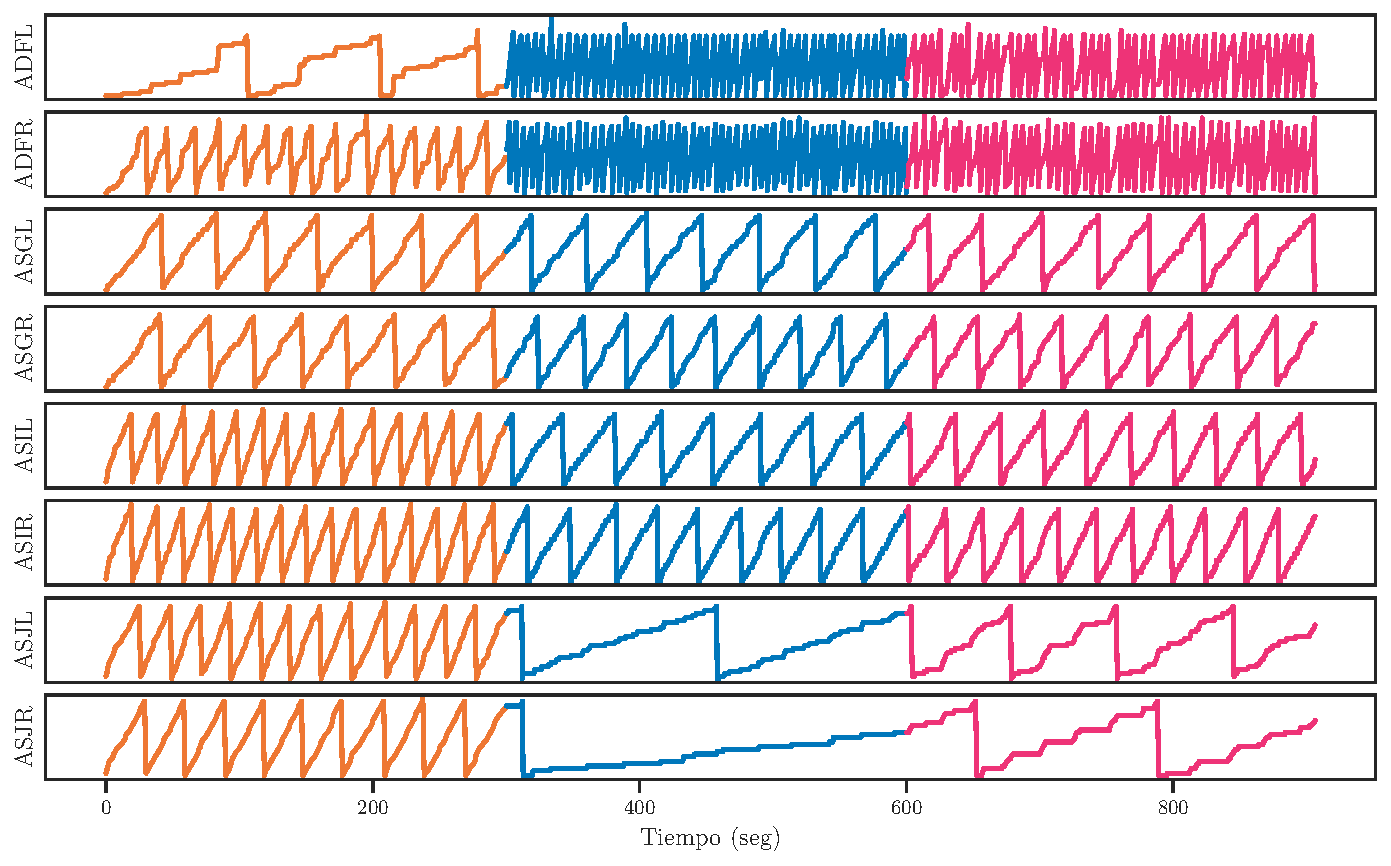
\includegraphics[width=\imsize]{intervalos_hambre.pdf}
	\caption[   Dinámica Neuronal de las Neuronas del Hambre en Tres Intervalos de Tiempo. ]{  Dinámica Neuronal de las Neuronas del Hambre en Tres Intervalos de Tiempo. La figura muestra cómo la frecuencia de oscilación de neuronas como ADFL(R), ASIL(R), y ASJL(R) varía en respuesta a diferentes entornos. El intervalo en el que el robot se encuentra frente a un obstáculo se destaca en azul, revelando cambios notables en la dinámica neuronal debido a la alteración del ambiente. }\label{fig:intervalos_hambre}
\end{figure}

En el segundo intervalo, se estimularon las neuronas de percepción táctil en la nariz, que incluyeron FLPR(L), ASHL(R), IL1VL(R), OLQDL(R) y OLQVR(L). Estas neuronas desencadenan movimientos de retroceso en el C. elegans en caso de colisión con un objeto. Tres clases de neuronas mecanosensoriales (ASH, FLP y OLQ) operan en paralelo para mediar esta respuesta, contribuyendo en fracciones distintas a la respuesta global: ASH (45\%), FLP (29\%) y OLQ (5\%). Las respuestas restantes ($\sim$10\%) son mediadas por las neuronas ALM y AVM, que detectan el tacto en la parte anterior del cuerpo. En el experimento con el robot, cuando se enfrenta a una pared y se activan estas neuronas, el robot ejecuta movimientos de retroceso para evitar el obstáculo. La \Cref{fig:intervalos_nariz} ilustra la actividad de estas neuronas, con el intervalo en el que el robot se encuentra frente a un obstáculo coloreado de azul. Al igual que en el caso de las neuronas del hambre, el impacto de la pared provoca un aumento en la frecuencia de algunas neuronas, como FLPR(L), ASHL, IL1VL(R) y OLQDL(R), mientras que ASHR mantiene su actividad inalterada. El último intervalo de tiempo refleja un comportamiento similar al descrito en el apartado anterior, donde el robot se adapta al entorno. Este intervalo se identifica visualmente mediante el color rosa.

\begin{figure}[h!]
	\centering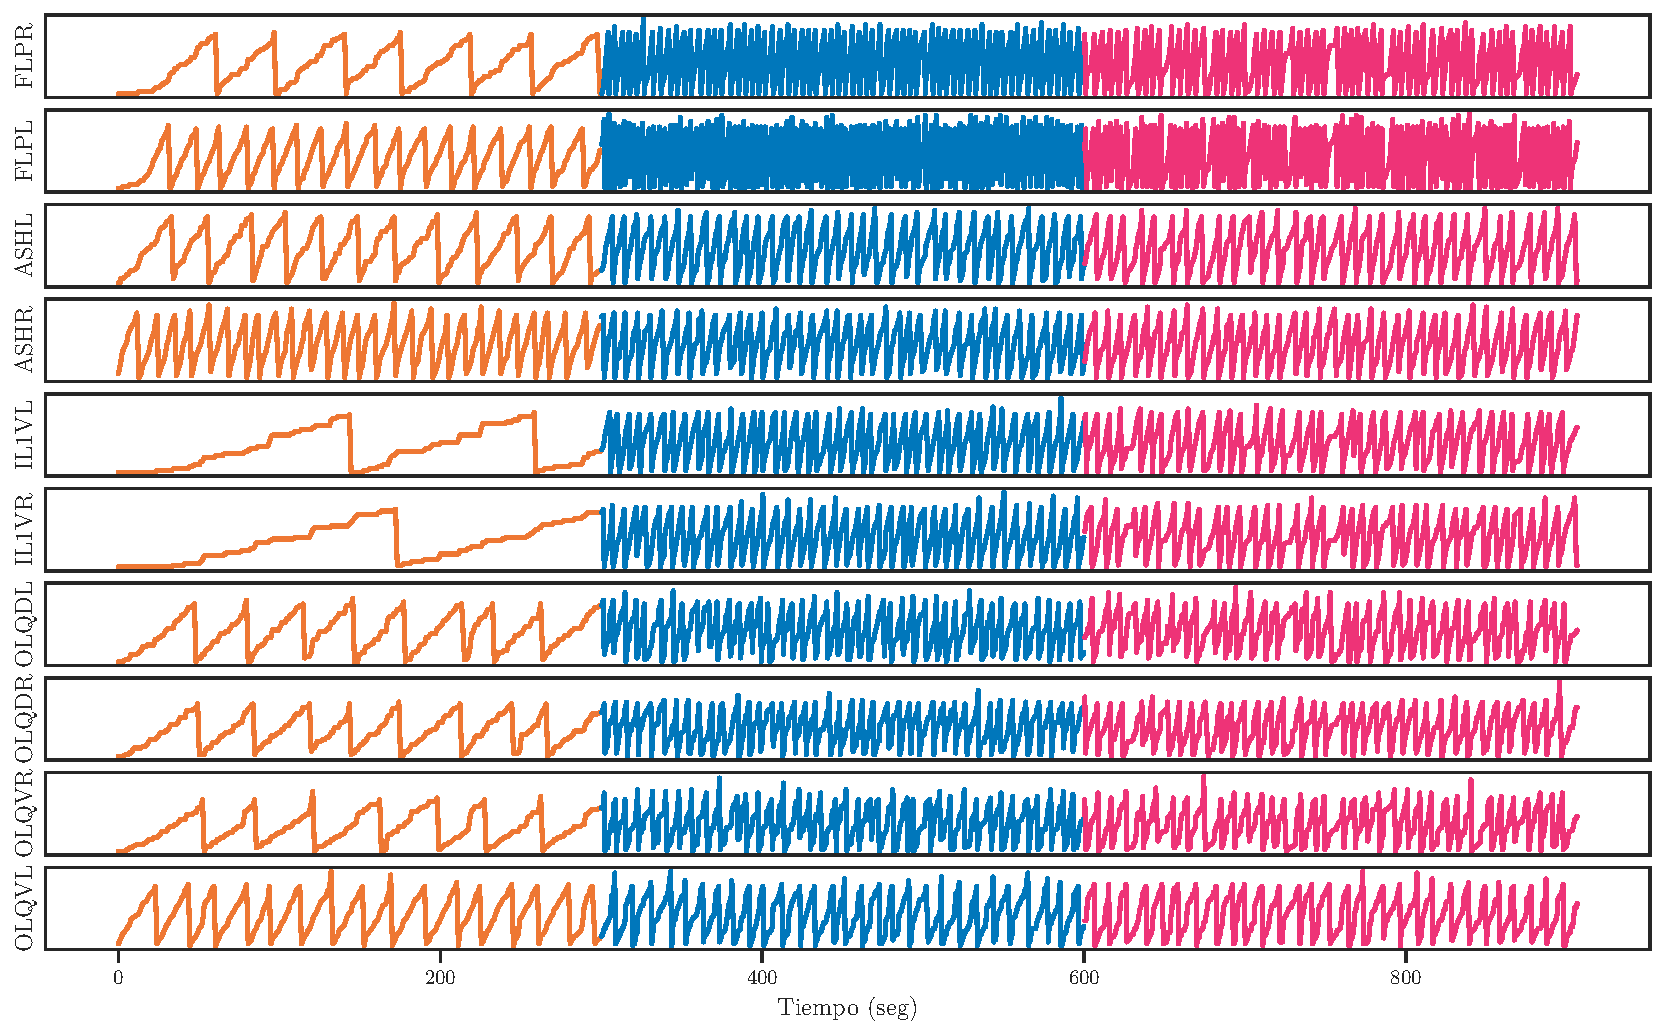
\includegraphics[width=\imsize]{intervalos_nariz.pdf}
	\caption[    Actividad Neuronal en el Segundo Intervalo con Estimulación de Neuronas de Tacto en la Nariz.  ]{   Actividad Neuronal en el Segundo Intervalo con Estimulación de Neuronas de Tacto en la Nariz.  En el intervalo en el que el robot se coloca frente a un obstáculo (resaltado en azul), se observa cómo las neuronas, como FLPR(L), ASHL, IL1VL(R), y OLQDL(R), experimentan cambios en su frecuencia de actividad en respuesta a la percepción táctil. La neurona ASHR, en cambio, mantiene su actividad constante.}\label{fig:intervalos_nariz}
\end{figure}

Para validar que el comportamiento emergente del robot se asemeja a lo observado en la biología del C. elegans, registramos las frecuencias de las acciones de avance, retroceso y rotación en la duración de los dos primeros intervalos. En el primer intervalo, donde solo se estimularon las neuronas del hambre (intervalo 1), predominaron las acciones de avanzar, en línea con la tendencia de los gusanos reales a explorar en busca de alimentos cuando se encuentran en un entorno rico en comida. En el caso de nuestro neuro-robot, el comportamiento fue análogo, con la mayor parte del tiempo destinado a avanzar y girar, explorando el espacio. Este patrón se refleja en las barras de la \Cref{fig:intervalo_comportamiento}a, donde las acciones relacionadas con el avance son más frecuentes que las demás. Por otro lado, en el segundo intervalo, se sabe que los gusanos reales tienden a huir de cualquier contacto, debido a su exposición a depredadores, como lo demuestran experimentos con pelos microscópicos. Por lo tanto, se esperaba que las acciones predominantes fueran las de retroceso, lo que se confirma en la \Cref{fig:intervalo_comportamiento}b, donde las acciones relacionadas con el retroceso son las más frecuentes.  Estos resultados indican que la dinámica cerebral modula el comportamiento del robot en función de las neuronas estimuladas, lo que refleja la adaptación del robot al entorno.

\begin{figure}[h!]
	\centering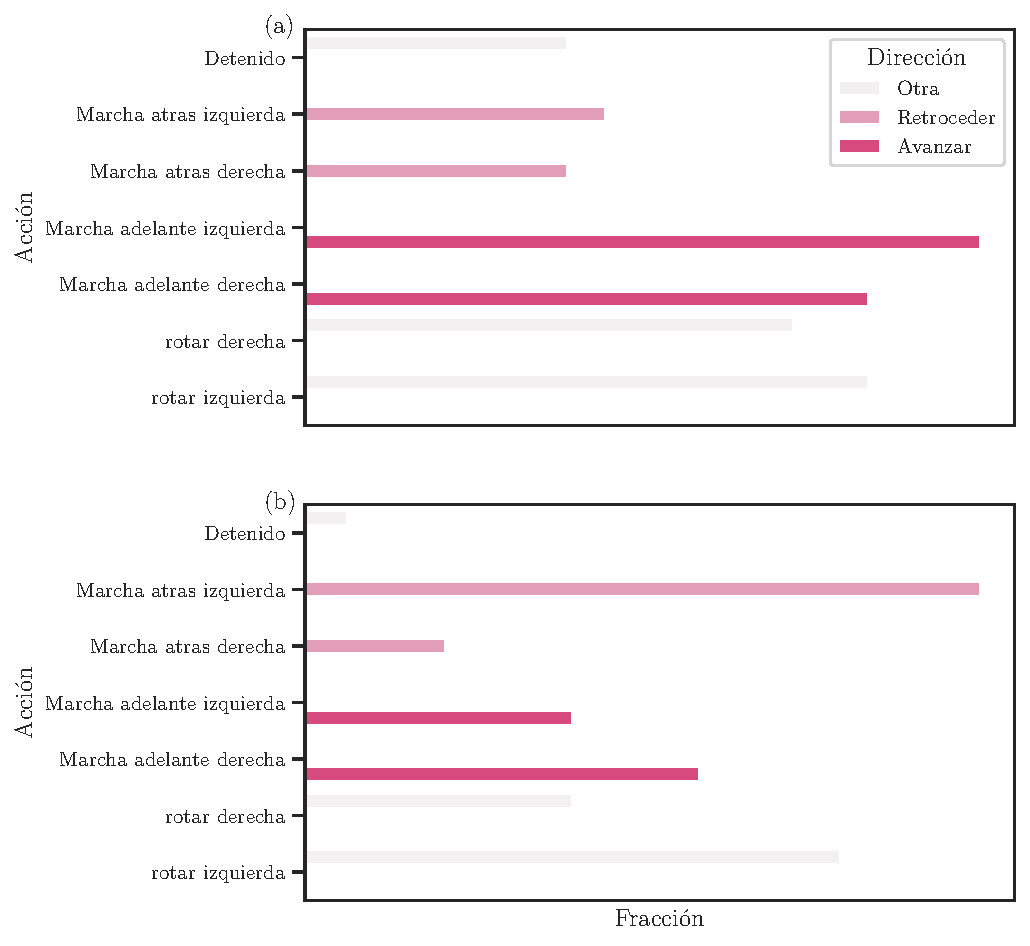
\includegraphics[width=\imsize]{fraccion_acciones.pdf}
	\caption[  Frecuencia de Acciones del Robot en el Primer y Segundo Intervalo.]{ Frecuencia de Acciones del Robot en el Primer y Segundo Intervalo.  (a) En el intervalo 1, con solo la estimulación de las neuronas del hambre, predominan las acciones de avanzar, reflejando la exploración en busca de alimentos, similar a lo observado en gusanos reales en entornos ricos en comida. (b) En el intervalo 2, cuando se estimulan las neuronas de percepción táctil en la nariz, las acciones de retroceso son prominentes, concordando con la tendencia de los gusanos reales a retroceder ante cualquier contacto debido a la presencia de posibles depredadores.}\label{fig:intervalo_comportamiento}
\end{figure}




\subsection{Discusión}

A pesar de contar únicamente con dos circuitos implementados en nuestro robot, hemos logrado obtener una amplia variedad de comportamientos complejos. Cabe destacar que en ningún momento se han programado órdenes específicas; en su lugar, se han activado los circuitos de mayor relevancia que previamente se habían identificado mediante ablación láser y otros experimentos. Para ampliar aún más el repertorio de comportamientos complejos, podríamos considerar la incorporación de más sensores y, basándonos en los hallazgos de la biología, activar los circuitos correspondientes. Por ejemplo, podríamos implementar un circuito relacionado con la detección de toques bruscos en el cuerpo a través de sensores táctiles. La implementación de hardware podría consistir en dos sensores táctiles, uno en la parte anterior y otro en la posterior del robot, cada uno con una entrada simple que puede estar "encendida" o "apagada". Cuando se presiona un sensor táctil, envía una señal de "encendido" que es leída por el programa de entrada. Si el sensor no se encuentra presionado (apagado), este envía una señal de "apagado". La activación de este sensor desencadenaría los circuitos relacionados con la percepción de toques bruscos, tanto en la parte anterior como en la posterior del robot. En el caso del C. elegans, la detección de toques bruscos en el cuerpo provoca una respuesta de retroceso marcada en el gusano. Sería interesante explorar si este modelo de conectoma puede reproducir el comportamiento cualitativo de orientación, tal como se investigó en el estudio de Morse et al. (1998), utilizando un sensor de luz.

El C. elegans localiza alimentos a través de la quimiotaxis, la capacidad de orientarse en respuesta a gradientes de concentración química. Sería valioso investigar si podemos observar un comportamiento de orientación similar a la quimiotaxis en nuestro modelo. Con un conjunto adecuado de sensores y una implementación precisa, podríamos estudiar circuitos neuronales asociados con comportamientos complejos en el robot de manera relativamente sencilla. Esto representa una ventaja significativa en comparación con los gusanos reales, ya que nos brinda acceso completo a la dinámica del sistema.

A pesar de las limitaciones actuales, este enfoque promete una mayor comprensión de los circuitos neuronales y del comportamiento emergente en los robots. Para lograr una mayor diversidad de comportamientos complejos, podríamos considerar la incorporación de más sensores y la activación de circuitos adicionales, lo que nos permitiría explorar una variedad de comportamientos complejos.





\section{La actividad neuronal global evoluciona en un colector de dimensión baja similar a un atractor}

La comprensión de cómo el sistema nervioso codifica, organiza y secuencializa los comportamientos es un pilar fundamental en la neurociencia de sistemas, ya sea al estudiar organismos tan simples como los gusanos o tan complejos como los seres humanos. En este contexto, nuestro estudio se enfoca en la evaluación de la relación entre la dinámica neuronal en el gusano C. elegans y su comportamiento, empleando técnicas experimentales afines a las utilizadas por Kato et al., cuyos resultados se presentan de manera resumida en la \Cref{sec:dinamicakato} y se ilustran en la \Cref{fig:kato}.

Con el propósito de abordar esta cuestión, llevamos a cabo un experimento que se extendió aproximadamente durante 20 minutos. Durante este período, el neurorobot emuló la actividad neuronal de C. elegans en el montaje experimental previamente descrito. Los datos resultantes comprenden 300 series temporales de datos dimensionales que detallan la actividad neuronal, con una dimensión asociada a cada neurona. La complejidad inherente de estos datos plantea un desafío inicial para su comprensión, lo que motiva la necesidad de un análisis más sofisticado.

En la \Cref{fig:matrizrobot}, se presenta la matriz de actividad que captura la dinámica neuronal del robot. Para identificar grupos de neuronas sincronizadas, implementamos un algoritmo de agrupación jerárquica utilizando la función \textbf{clustermap} de la biblioteca Seaborn. Esta aproximación nos permitió de manera efectiva visualizar la estructura subyacente en los datos y discernir los patrones de sincronización neuronal que son esenciales para comprender la relación entre la actividad neuronal y el comportamiento del neurorobot.


 \begin{figure}[h!]
	\centering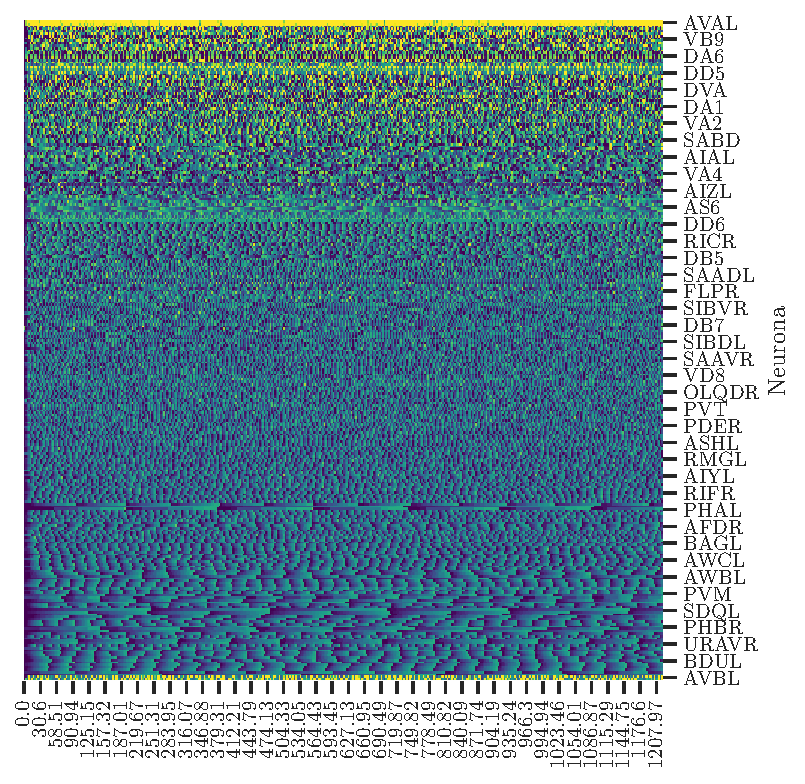
\includegraphics[width=\imsize]{clusteres_dinamica.pdf}
	\caption[ Matriz de Actividad que Representa la Dinámica Neuronal del Neurorobot.]{ Matriz de Actividad que Representa la Dinámica Neuronal del Neurorobot. Se muestra la matriz de actividad que refleja la dinámica neuronal del neurorobot durante el experimento. Cada entrada de la matriz corresponde a la actividad de una neurona en un instante de tiempo específico. Utilizando un algoritmo de agrupación jerárquica, se identificaron patrones de sincronización entre las neuronas, lo que proporciona una visión crucial de la coordinación neuronal en el sistema. Este análisis de la dinámica neuronal es fundamental para comprender la relación entre la actividad neuronal y el comportamiento emergente del neurorobot.}\label{fig:matrizrobot}
\end{figure}



 \begin{figure}[h!]
	\centering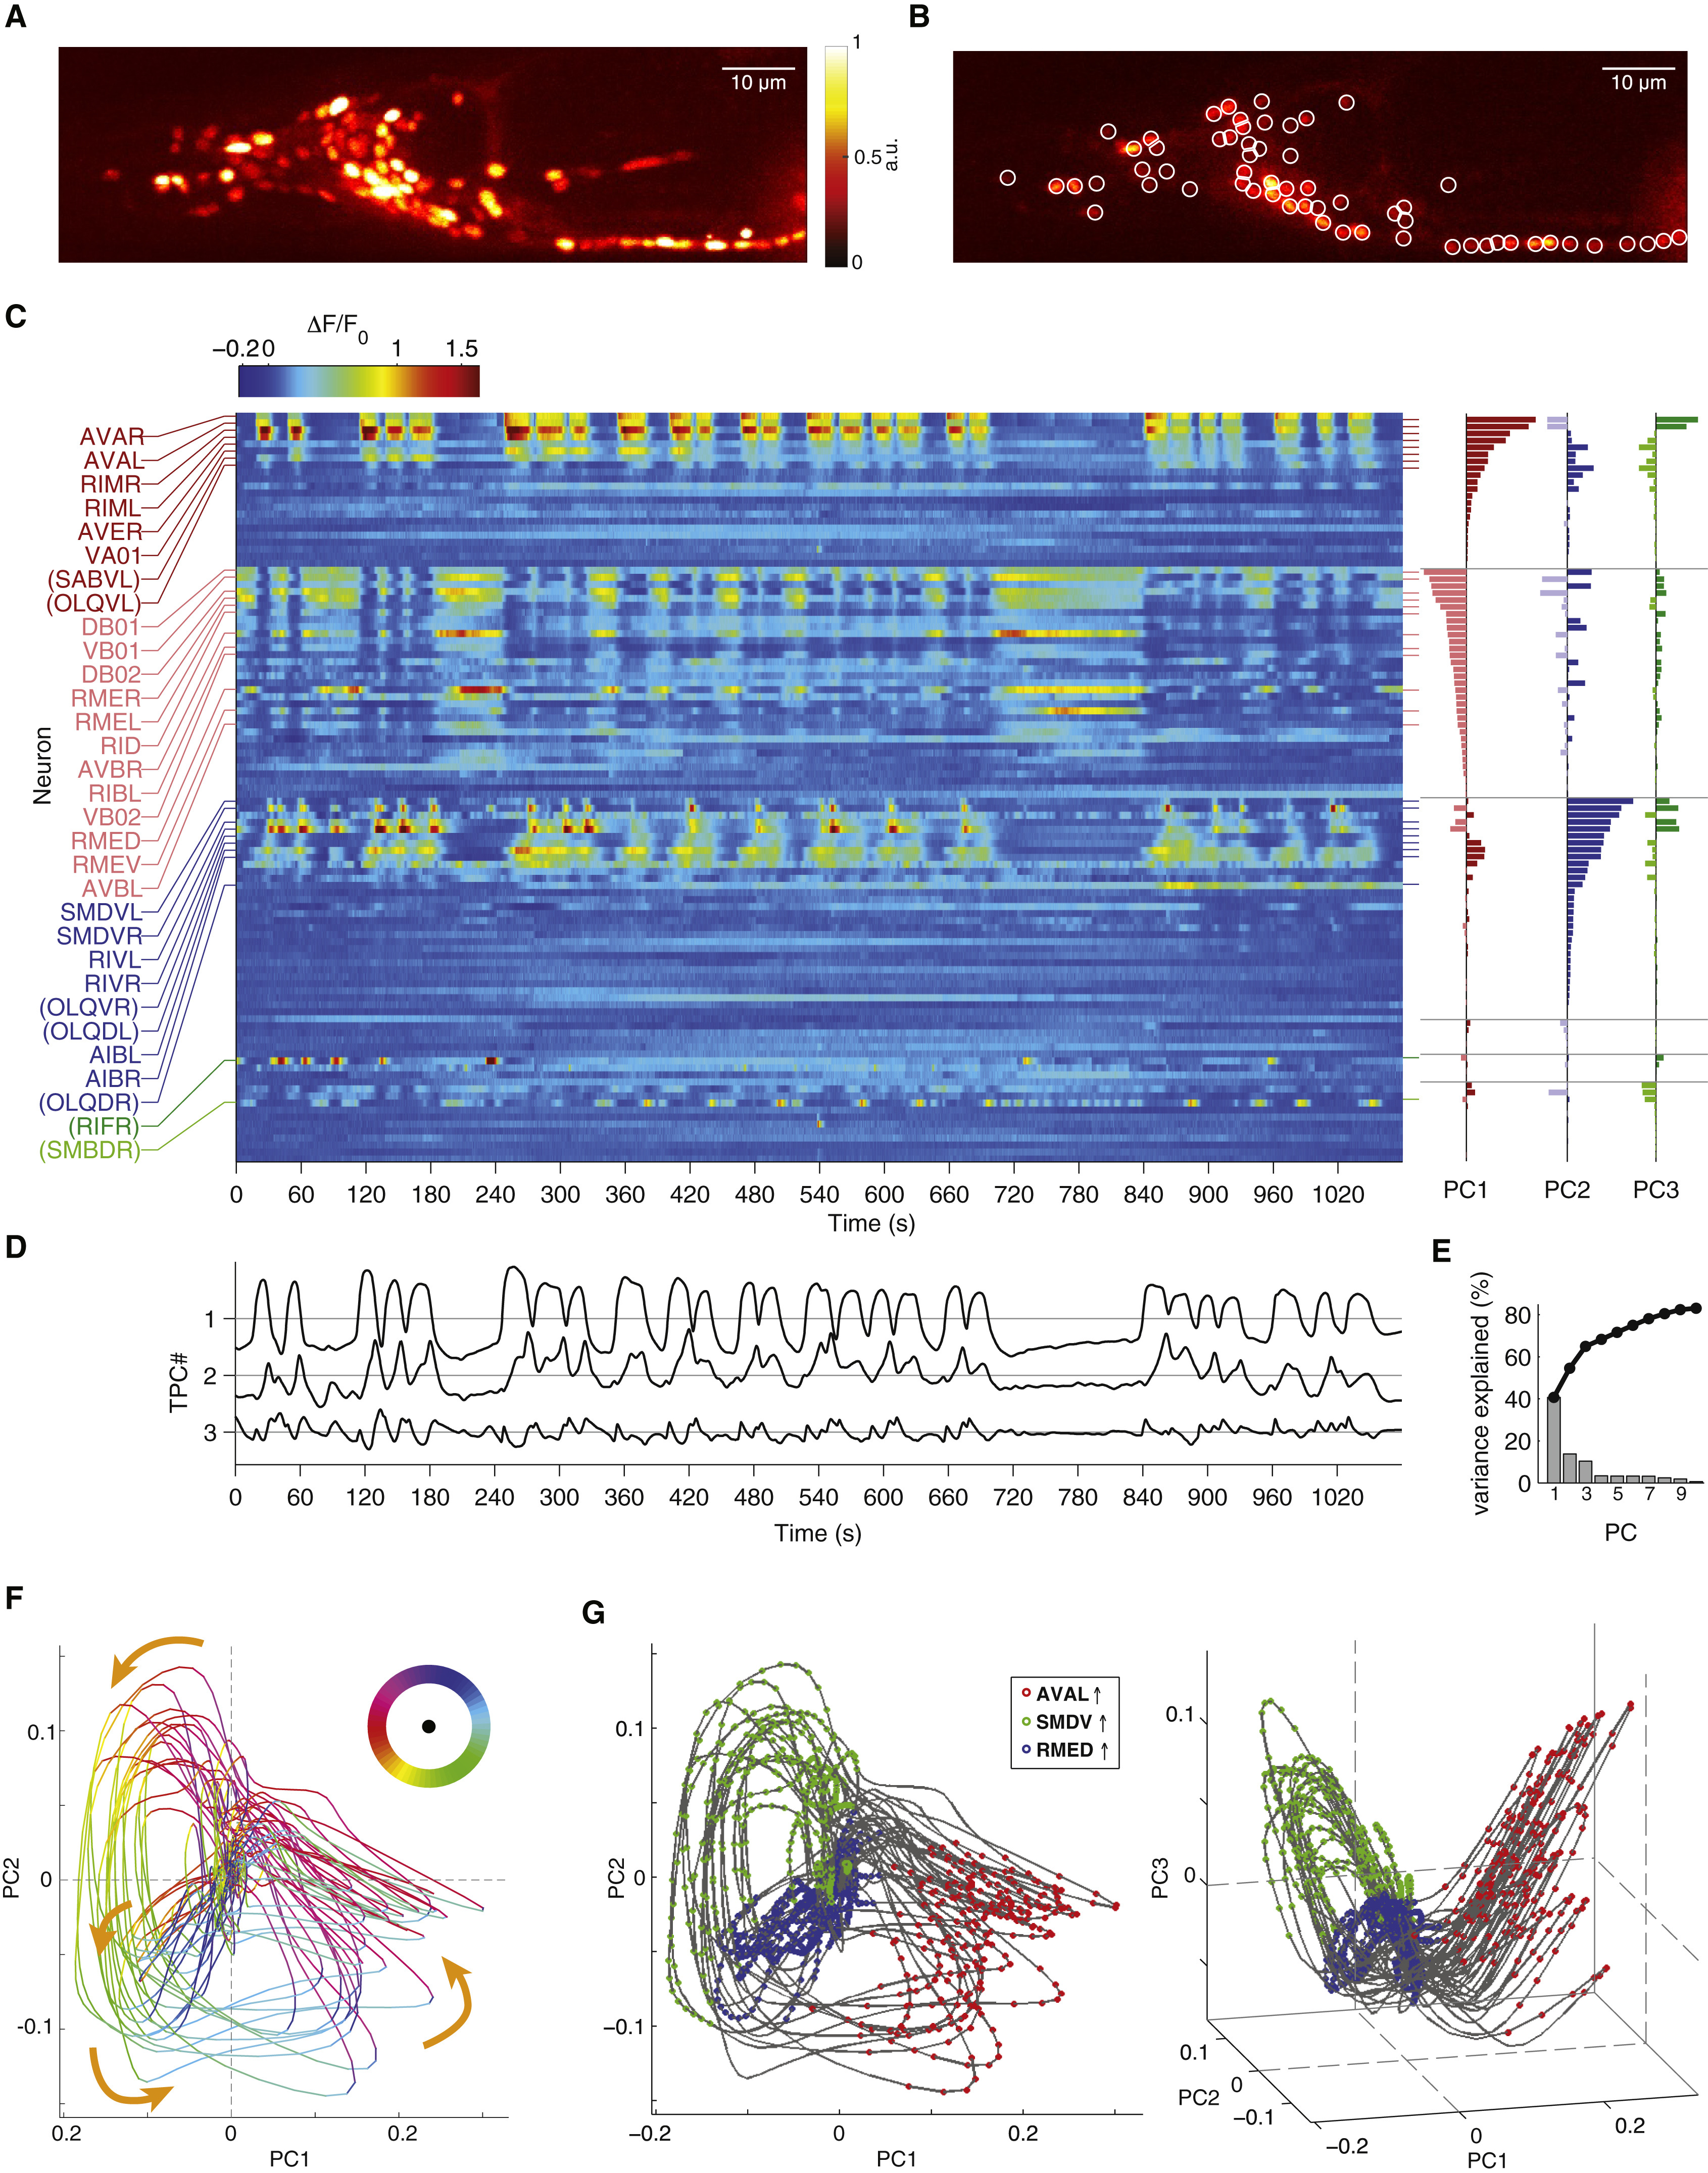
\includegraphics[width=\imsize]{kato.jpg}
	\caption[ La actividad cerebral se organiza en una trayectoria de espacio de estado neural cíclico de baja dimensión en gusanos reales.]{ La actividad cerebral se organiza en una trayectoria de espacio de estado neural cíclico de baja dimensión en gusanos reales.  (A) Proyección de máxima intensidad de una muestra representativa grabada en condiciones constantes.
		(B) Plano z único superpuesto con regiones neuronales segmentadas.
		(C) Mapa de calor de las series de tiempo de fluorescencia ($\Delta F/F$) de 109 neuronas cefálicas segmentadas, una neurona por fila.  Las neuronas están coloreadas y agrupadas por sus pesos y signos de componentes principales (PC1-3), que se muestran en los gráficos de barras de la derecha. (D) Integrales de los tres primeros PC temporales. (E) Varianza explicada por los primeros diez PC, la línea negra indica la varianza acumulada explicada. 		(F) Diagrama de fase de los dos primeros PC temporales coloreados por la dirección de la evolución temporal indicada por la leyenda de colores. (G) Diagramas de fase de los dos primeros (izquierda) y los tres primeros (derecha) PC temporales. }\label{fig:kato}
\end{figure}




 Dado que los datos son ruidosos, aplicamos una derivada temporal a nuestra matriz de actividad neuronal, utilizando una derivada regularizada (\Cref{eq:ap:2}) con un parámetro de regularización $\alpha$ de 2 (\Cref{fig:derivada_regularizada}). Luego, estandarizamos los datos, lo que implica transformarlos para que sigan una distribución normal estándar (gaussiana) con una media de cero y una varianza unitaria. Esta estandarización es un requisito común para muchos algoritmos de aprendizaje automático, como el Análisis de Componentes Principales (PCA).  Luego de estandarizar los datos, realizamos un análisis de componentes principales (PCA) de las derivadas temporales de las trazas normalizadas, lo que nos permitió proyectar los datos originales de 301 dimensiones en tres dimensiones. Estos nuevos componentes representan las tres dimensiones principales de la variación, como se ilustra en la \Cref{fig:pcs}. Además, para cada componente principal (PC), generamos una serie temporal correspondiente (PC temporal) al calcular la media ponderada de la serie temporal multineural completa. Los PC temporales capturan señales compartidas por neuronas que se agrupan en función de sus correlaciones. De manera sorprendente, descubrimos que los tres primeros PC explicaban el 30 \% de la varianza total en nuestros datos, como se muestra en la \Cref{fig:varianza}.
 
 
  \begin{figure}[h!]
 	\centering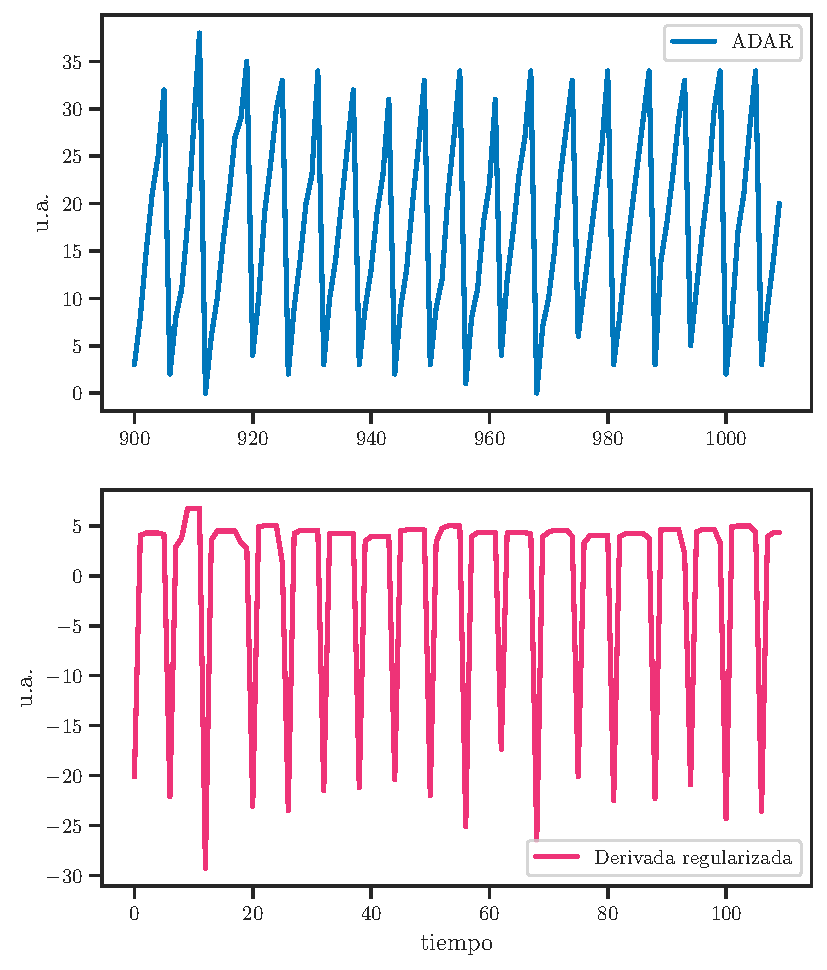
\includegraphics[width=\imsize]{derivada_robot.pdf}
 	\caption[Ejemplo de aplicar la derivada regularizada a una neurona del experimento.]{Ejemplo de aplicar la derivada regularizada a una neurona del experimento.}\label{fig:derivada_regularizada}
 \end{figure}
 
 
 \begin{figure}[h!]
 	\centering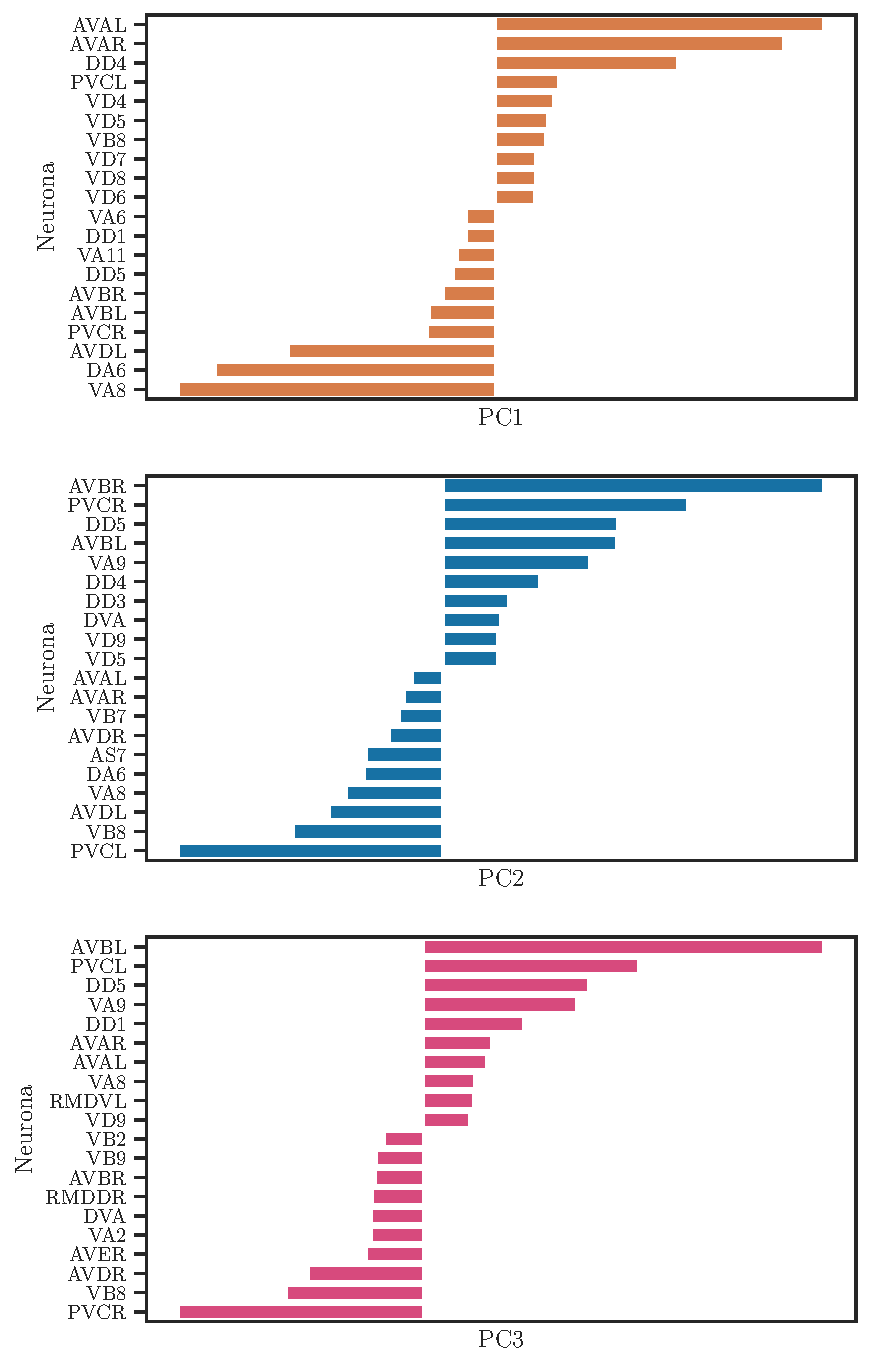
\includegraphics[width=\imsize]{PCs_robot.pdf}
 	\caption[Las neuronas están ordenas y agrupadas por sus pesos y signos de componentes principales (PC1-3).]{Las neuronas están ordenas y agrupadas por sus pesos y signos de componentes principales (PC1-3). (a) Coeficientes PC1, agrupados por orden de pesos. (b) Coeficientes PC2, (c) Coeficientes PC3.}\label{fig:pcs}
 \end{figure}


 \begin{figure}[h!]
	\centering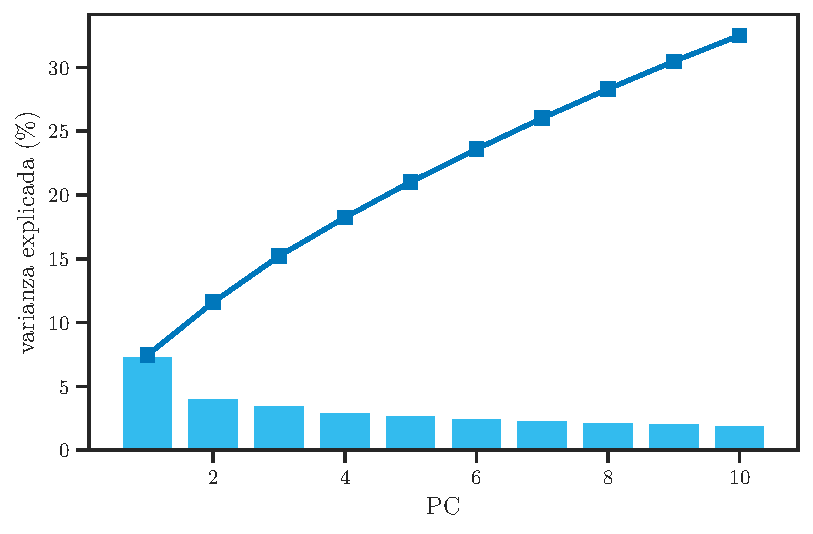
\includegraphics[width=\imsize]{varianza_explicada_robot.pdf}
	\caption[Varianza explicada por las primeros diez componentes principales, la línea azul oscuro indica la varianza acumulada explicada.]{Varianza explicada por las primeros diez componentes principales, la línea azul oscuro indica la varianza acumulada explicada.}\label{fig:varianza}
\end{figure}


La integral de tiempo del primer PC temporal mostró un patrón oscilatorio con variaciones en el tiempo, transiciones abruptas y períodos estables (\Cref{fig:ingegral_PCS}). Este patrón se deriva de la interacción entre dos grupos de interneuronas y neuronas motoras, previamente implicados en el control de la locomoción dirigida hacia adelante y hacia atrás. Notamos que las neuronas que anteriormente desempeñaban funciones opuestas tenían signos opuestos en sus pesos del primer PC (ver \Cref{fig:pcs} ; p. ej., AVA promueve el rastreo hacia atrás y AVB promueve el rastreo hacia adelante). En contraste, el segundo y tercer PC recibieron contribuciones significativas de las neuronas motoras de la cabeza, aunque sus pesos neuronales indicaron contribuciones de múltiples neuronas. Los patrones y contribuciones de los PC1 a PC3 se mantuvieron consistentes en múltiples repeticiones del experimento.


 \begin{figure}[h!]
	\centering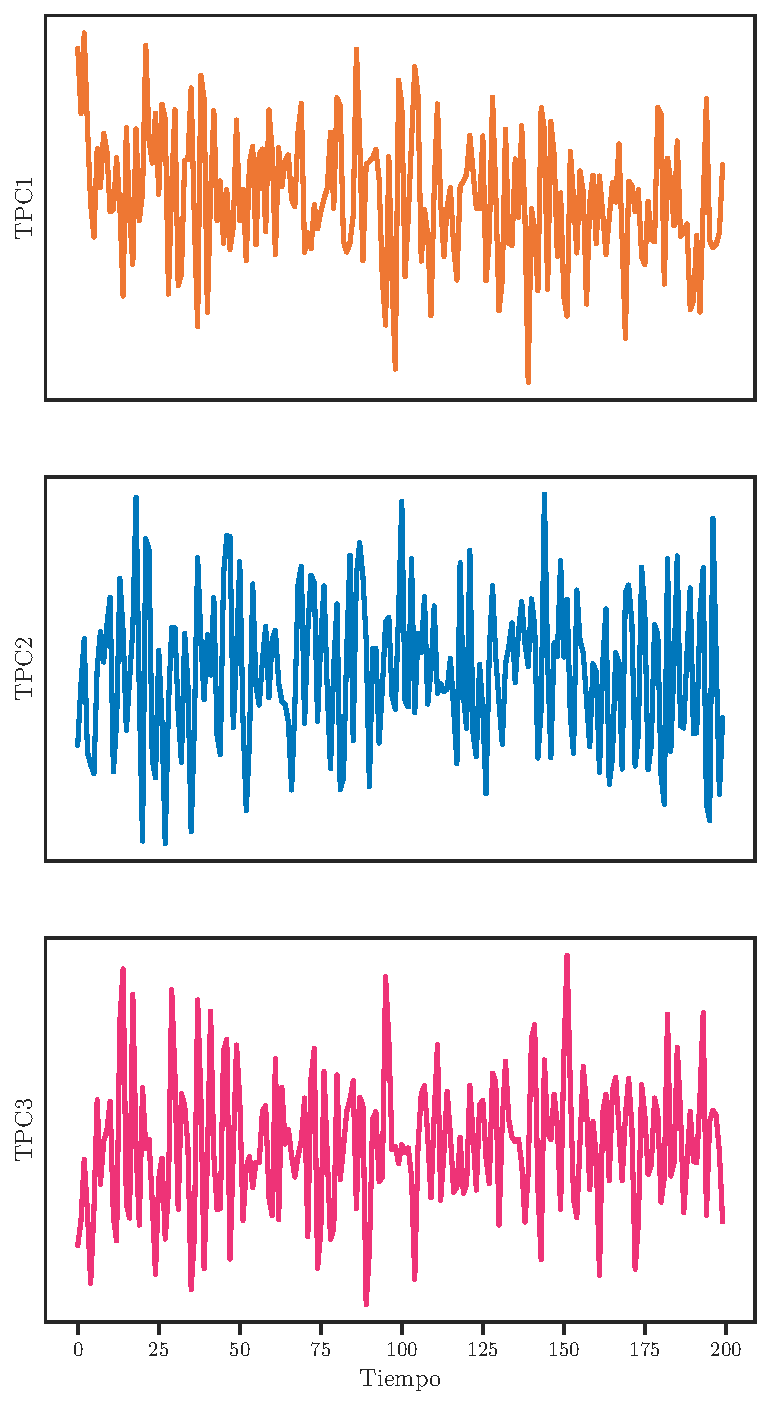
\includegraphics[width=\imsize]{TPCs_robot.pdf}
	\caption[ Integrales de los primeros tres PC temporales.]{ Integrales de los primeros tres PC temporales.}\label{fig:ingegral_PCS}
\end{figure}

El diagrama de fase de los PC1-3 (\Cref{fig:colector}) temporales mostró resultados similares a los de Kato et al. (\Cref{fig:kato}), en los que la evolución temporal del estado neural era cíclica, con estados que se repetían en cada ensayo. Estos ciclos de trayectoria formaban paquetes espacialmente coherentes en el espacio PCA. En consecuencia, toda la trayectoria del estado neural trazó un colector que definimos como el \textquote{subvolumen del espacio PCA ocupado por la trayectoria del estado neural}.  El hallazgo más destacado fue que, de manera similar a los resultados previos, la trayectoria del estado neural trazaba un conjunto que correspondía a diferentes comportamientos de locomoción. Estos comportamientos estaban asociados con la matriz de acciones realizadas por el robot (ver \Cref{fig:acciones}), donde cada trayectoria se relacionaba con una acción específica, representada por un color en nuestra visualización. Es importante destacar que las figuras anteriores se suavizaron mediante interpolación numérica. Nuestros resultados sugieren que la dinámica neural puede ser utilizada para predecir el comportamiento de un gusano C. elegans. Esto abre nuevas posibilidades para el desarrollo de robots bioinspirados que imitan el comportamiento de los animales.


 \begin{figure}[h!]
	\centering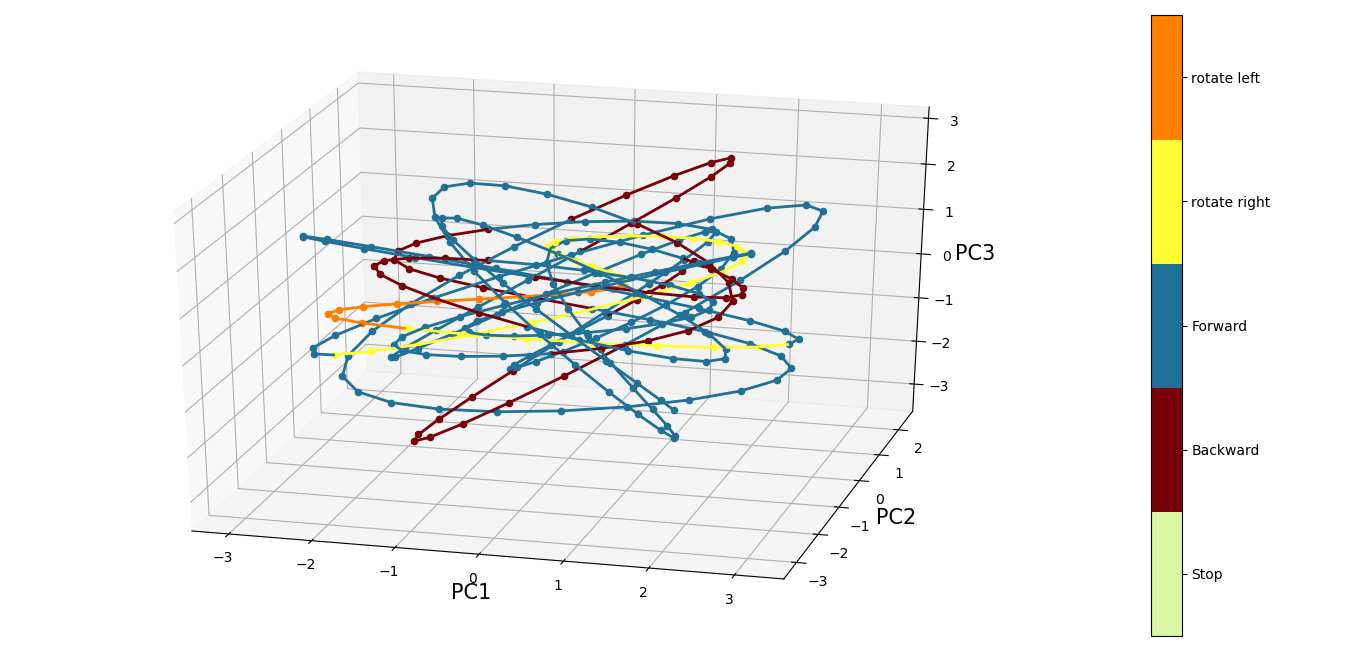
\includegraphics[width=\imsize]{PCs.png}
	\caption[ Dinámica neural global y acciones. Diagramas de fase de los tres primeros PC temporales en un intervalo de tiempo seleccionado.  ]{Dinámica neural global y acciones. Diagramas de fase de los tres primeros PC temporales en un intervalo de tiempo seleccionado. Las acciones del robot se representan con diferentes colores. La figura muestra que la dinámica global evoluciona en una órbita similar a un atractor de baja dimensión, donde diferentes segmentos de la trayectoria corresponden a estados motores bien definidos.}\label{fig:colector}
\end{figure}


 \begin{figure}[h!]
	\centering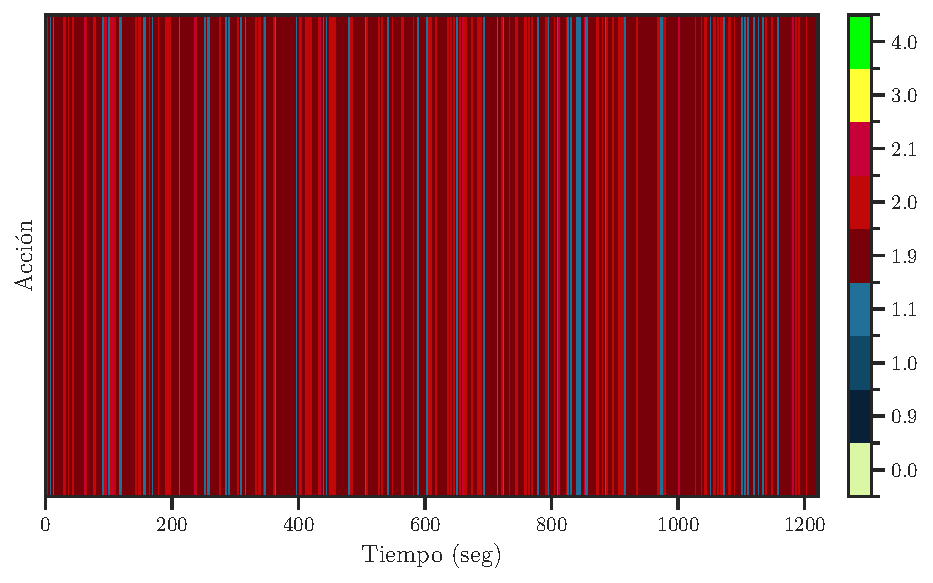
\includegraphics[width=\imsize]{accion_robot.pdf}
	\caption[ Matriz de acciones realizadas por el robot]{Matriz de acciones realizadas por el robot.}\label{fig:acciones}
\end{figure}


 \begin{figure}[h!]
	\centering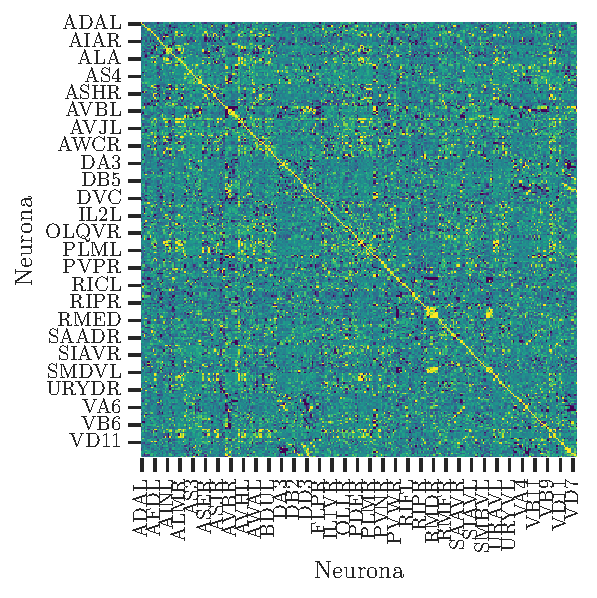
\includegraphics[width=\imsize]{correlacion_robot.pdf}
	\caption[ Correlación de Activación entre Neuronas.]{Correlación de Activación entre Neuronas.  En amarillo, se resaltan las neuronas que presentan correlación significativa, indicando que la dinámica global del robot se organiza en grupos o clústeres de neuronas. Esto sugiere una actividad de red rica y coordinada.}\label{fig:correlacion_robot}
\end{figure}

\subsection{Discusión}

Esta sección se centro en  la dinámica global y su relación con la acción. Al igual que \cite{kato_global_2015}, construimos series temporales de PC temporales tomando promedios ponderados de cada componente principal con la serie temporal mulineuronal completa. Esto permite una reducción drástica de la dimensionalidad, donde las PC temporales tienen señales que son representativas de grupos neuronales. La \Cref{fig:correlacion_robot} muestra un mapa de calor que representa la correlación de activación entre las neuronas en el robot. Las áreas coloreadas en amarillo indican que ciertas neuronas están correlacionadas, lo que sugiere una organización en grupos o clústeres de neuronas en la dinámica del robot. Esta correlación de actividad neuronal resalta la existencia de una red neuronal rica y coordinada en el sistema, lo que puede tener implicaciones significativas en la generación de comportamientos emergentes y adaptativos en el robot.

En la \Cref{fig:colector}  mostramos una representación paramétrica de las integrales temporales de las tres primeras PC temporales en un intervalo de tiempo fijo. La trayectoria presenta un comportamiento similar al de un sistema dinámico en una órbita tipo atractor. Además, encontramos que las trayectorias de la serie temporal completa de los experimentos siempre presentaban este comportamiento, y permanecían acotadas en un estado global caracterizado por la presencia de órbitas cíclicas.

Cuando se tuvo en cuenta la actividad del robot, encontramos que diferentes segmentos de las trayectorias corresponden a diferentes acciones. Esto se puede ver claramente en la \Cref{fig:colector}, donde utilizamos diferentes colores para representar la acción que el robot estaba ejecutando en un momento dado. Elegimos un segmento de tiempo particular en el que el robot se encuentra con un obstáculo, se detiene, retrocede y giraba. Obsérvese que las diferentes acciones pueden distinguirse claramente como segmentos bien definidos de la trayectoria.

En C. elegans, Kato et al. \cite{kato_global_2015} encontraron que la actividad neuronal evoluciona en una variedad de baja dimensión similar a un atractor. Además, diferentes segmentos en esta variedad, que corresponden a la sincronización de diferentes grupos de neuronas, están claramente correlacionados con diferentes estados motores. Nuestros resultados destacan el papel que juega el connectoma en la emergencia de estos estados cíclicos tipo atractor.




\section{Dinámicas neuronales emergentes}

 \subsection{ Sincronización de frecuencia y fase}

En este apartado analizaremos la correlación entre la dinámica global y el conectoma subyacente. Vale la pena destacar que en el modelo robótico, todas las neuronas tienen el mismo umbral de disparo y, por lo tanto, tienen dinámicas individuales idénticas como unidades aisladas. Sin embargo, esperamos que sus dinámicas reflejen la distribución no uniforme de la conectividad sináptica. Por ejemplo, las neuronas en una posición central, con un gran número de entradas o conexiones con pesos grandes, pueden alcanzar el umbral más rápido y, por lo tanto, disparar con frecuencia. De hecho, descubrimos que AVAL, AVBR y AVBL, nodos con la mayor centralidad de grado y también con la mayor centralidad de cercanía \cite{varshney_structural_2011}, oscilan con alta frecuencia. En contraste, los nodos en una posición periférica reciben menos entradas y, por lo tanto, tardarán más en alcanzar el umbral, lo que conduce a una dinámica más lenta. En la \Cref{fig:sincronia_1}A representamos las señales de tres neuronas motoras del cordón ventral en un intervalo de tiempo fijo, mostrando oscilaciones a diferentes frecuencias. Caracterizamos cuantitativamente estas oscilaciones realizando una transformada de Fourier (FT; \Cref{fig:sincronia_1}B). Encontramos que el valor real de la FT presenta picos definidos y, por lo tanto, definimos la frecuencia característica de las neuronas, $\Omega$, como el pico más alto en la FT.


 \begin{figure}[h!]
	\centering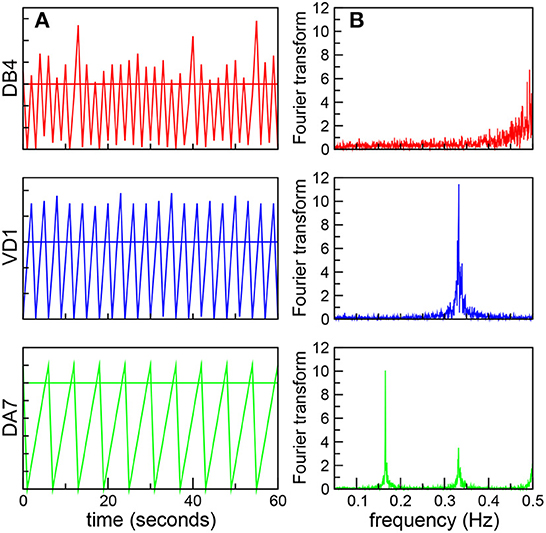
\includegraphics[width=\imsize]{sincronia1.jpg}
	\caption[ Las neuronas oscilan a diferentes frecuencias.]{Las neuronas oscilan a diferentes frecuencias. (A) Dinámica de tres neuronas motoras del cordón ventral, DB4 (arriba, rojo), VD1 (medio, azul) y DA7 (abajo, verde). La figura muestra las señales neuronales en función del tiempo en el mismo intervalo de tiempo de 60 segundos. Las líneas horizontales muestran el valor umbral h = 30. (B) Transformadas de Fourier correspondientes con picos definidos, utilizados para definir la frecuencia característica $\Omega$.}\label{fig:sincronia_1}
\end{figure}

Como se discutió en el \Cref{sec:kato}  Kato et al.\cite{kato_global_2015} registraron experimentalmente grupos de neuronas que presentan dinámicas coordinadas en C. elegans.  Con esta idea en mente, cuando extendemos nuestro enfoque de la dinámica individual a la colectiva, observamos que algunas neuronas se agrupan en grupos que comparten la misma frecuencia característica. Incluso más, en algunos casos la forma completa de su transformada de Fourier (FT), incluidos los picos más pequeños, se superpone. Esto nos permite definir grupos sincronizados como grupos de neuronas con FTs superpuestas.

 \begin{figure}[h!]
	\centering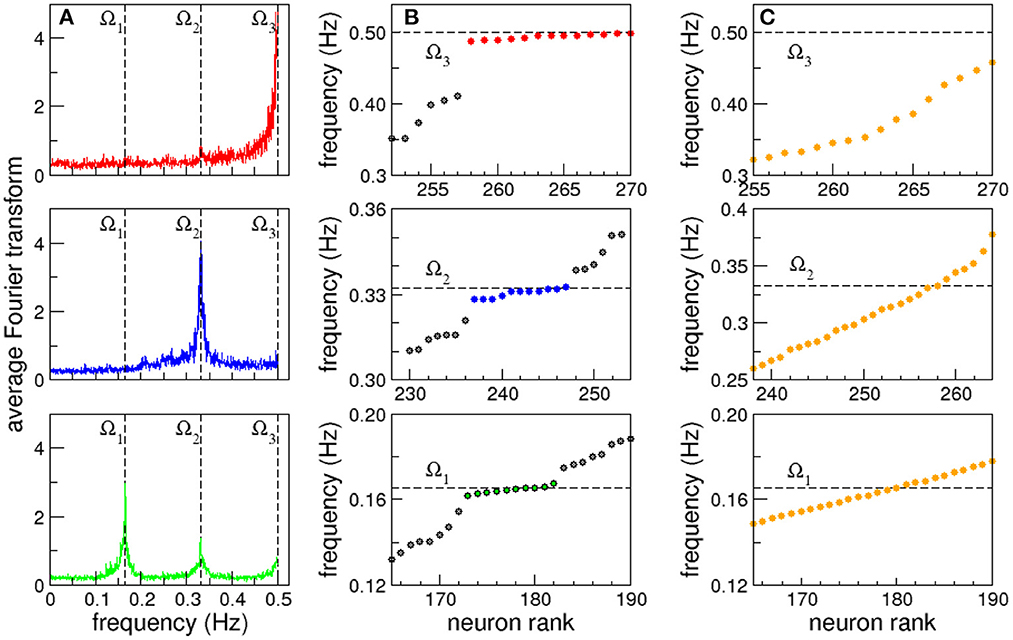
\includegraphics[width=\imsize]{sincronia2.jpg}
	\caption[ Sincronización de frecuencias.]{Sincronización de frecuencias. (A) Transformadas de Fourier promedio de las neuronas en tres grupos sincronizados para un experimento completo de 15 minutos de duración. (B) Neuronas ordenadas de menor a mayor frecuencia característica. Las líneas discontinuas se muestran como una guía para el ojo para mostrar la frecuencia característica de los grupos sincronizados que aparecen como líneas horizontales. (C) No se observan grupos sincronizados en los experimentos de control con versiones aleatorias del  conectoma.}\label{fig:sincronia_2}
\end{figure}

En la \Cref{fig:sincronia_2}A, trazamos la transformada de Fourier promedio de las neuronas en tres grupos sincronizados de frecuencia diferente. Las transformadas de Fourier promediadas tienen picos agudos, que nos permiten definir los grupos $\Omega$ por su frecuencia característica (media $\pm$ desviación estándar): $\Omega_1 = 0.165 \pm 0.002$ Hz (verde, inferior), $\Omega_2 = 0.332 \pm 0.003$ Hz (azul, medio) y $\Omega_3 = 0.496 \pm 0.004$ Hz (rojo, superior; consulte también las  \Cref{table:cluster_1,table:cluster_2,table:cluster_3} y las \Cref{fig:cluster_1,fig:cluster_2,fig:cluster_3} para una lista completa de neuronas en cada grupo, sus señales individuales y las FT correspondientes). Tenga en cuenta que $\Omega_2$ y $\Omega_3$ son aproximadamente múltiplos enteros de $\Omega_1$. Si bien el origen de tal relación armónica aparente aún no está claro, tener solo tres frecuencias no puede excluirse una coincidencia aleatoria. La \Cref{fig:sincronia_2}B muestra en detalle los tres grupos sincronizados cuando las neuronas se ordenan de menor a mayor frecuencia característica. Usamos líneas discontinuas como una guía para el ojo para mostrar las frecuencias características $\Omega$ de los grupos sincronizados que aparecen como líneas horizontales. En este punto, vale la pena enfatizar que la aparición de grupos sincronizados no parece depender de la topografía particular donde se mueve el robot. Esto se debe al hecho de que las neuronas sensoriales asociadas con el comportamiento de evitación solo se estimulan cuando el sensor de distancia mide una distancia por debajo del umbral y, dado que entonces el robot responde retrocediendo, el intervalo de tiempo en el que las neuronas sensoriales son estimuladas suele ser muy corto. Como consecuencia, la dinámica neuronal global converge rápidamente de nuevo a un atractor global.


 \begin{table}[h!]
	\centering
	\caption[La tabla  presenta las neuronas del grupo sincronizado $\Omega_1$, su descripción, la frecuencia característica correspondiente y el peso del primer componente principal (PC1). ]{ La tabla  presenta las neuronas del grupo sincronizado $\Omega_1$, su descripción, la frecuencia característica correspondiente y el peso del primer componente principal (PC1).  VCMN = Neurona motora del cordón ventral, 
		RVCI = Neurona interneuronal del anillo y el cordón ventral, RI = Neurona interneuronal del anillo.}
	\begin{tblr}{colspec={llll},
			row{odd} = {bg=gray8},
			row{even} = {bg=gray9},
			row{1} = {bg=red3, fg=white, font=\sffamily},
		}
		
Neurona & Descripción & $\Omega$  & PC1 \\
DA7  &  VCMN &  $0.166 \pm 0.001$ & $2.7 \pm 0.1$ \\
AVL  & RVCI & $0.164 \pm 0.001$ & $1.6 \pm 0.1$ \\
AS2 & VCMN & $0.163 \pm 0.001$ &  $0.1 \pm 0.1$ \\
DB4  & VCMN &  $0.165 \pm 0.001$ & $0.1 \pm 0.1$ \\
RMDL & VCMN & $0.167 \pm 0.001$ & $-0.2 \pm 0.1$ \\
VA7 & VCMN & $0.166 \pm 0.001$ & $-0.8 \pm 0.1$ \\
DD6 & VCMN & $0.166 \pm 0.001$ & $-1.2 \pm 0.1$ \\
SABVR & RI &  $0.162 \pm 0.001$ & $-4.2 \pm 0.1$\\
RID & RI & $0.164 \pm 0.001$ & $-7.1 \pm 0.1$\\
VD7 & VCMN & $0.165 \pm 0.001$ &  $-13.5 \pm 0.1$
	\end{tblr}
	\label{table:cluster_1}
\end{table}



\begin{table}[h!]
	\centering
	\caption[La tabla  presenta las neuronas del grupo sincronizado $\Omega_2$, su descripción, la frecuencia característica correspondiente y el peso del primer componente principal (PC1). ]{ La tabla  presenta las neuronas del grupo sincronizado $\Omega_2$, su descripción, la frecuencia característica correspondiente y el peso del primer componente principal (PC1).  VCMN = Neurona motora del cordón ventral}
	\begin{tblr}{colspec={llll},
			row{odd} = {bg=gray8},
			row{even} = {bg=gray9},
			row{1} = {bg=red3, fg=white, font=\sffamily},
		}
		
		Neurona & Descripción & $\Omega$  & PC1 \\
		VA11  &  VCMN &  $0.331 \pm 0.001$ & $15.3 \pm 0.1$ \\
		VA6  & VCMN & $0.331 \pm 0.001$ &  $9.8 \pm 0.1$ \\
		DA5 & VCMN &  $0.333 \pm 0.001$ &  $7.4 \pm 0.1$ \\
		VD3 & VCMN & $0.328 \pm 0.001$ &  $3.9 \pm 0.1$\\
		VD1  & VCMN& $0.330 \pm 0.001$ &  $0.6 \pm 0.1$ \\
		DA1 & VCMN & $0.332 \pm 0.001$ &  $-1.7 \pm 0.1$ \\
		AS11 & VCMN & $0.328 \pm 0.001$ & $-2.5 \pm 0.1$ \\
		DD3 & VCMN & $0.331 \pm 0.001$ &  $-6.4 \pm 0.1$ \\
		VD4 & VCMN & $0.328 \pm 0.001$ &  $-7.1 \pm 0.1$\\
		VD6 & VCMN &  $0.332 \pm 0.001$ &  $-12.7 \pm 0.1$\\	
		
	\end{tblr}
	\label{table:cluster_2}
\end{table}


\begin{table}[h!]
	\centering
	\caption[La tabla  presenta las neuronas del grupo sincronizado $\Omega_3$, su descripción, la frecuencia característica correspondiente y el peso del primer componente principal (PC1). ]{ La tabla  presenta las neuronas del grupo sincronizado $\Omega_3$, su descripción, la frecuencia característica correspondiente y el peso del primer componente principal (PC1).  VCMN = Neurona motora del cordón ventral, Interneurona del cordón ventral.}
	\begin{tblr}{colspec={llll},
			row{odd} = {bg=gray8},
			row{even} = {bg=gray9},
			row{1} = {bg=red3, fg=white, font=\sffamily},
		}
		
		Neurona & Descripción & $\Omega$  & PC1 \\
       VA8 & VCMN & $0.498 \pm 0.001$ & $110.1 \pm 0.1$\\
       DA6  & VCMN & $0.496 \pm 0.001$ & $95.8 \pm 0.1$\\
       AVDL & VCI & $0.496 \pm 0.001$ & $76.1 \pm 0.1$\\
       AS7 & VCMN  & $0.495 \pm 0.001$ & $29.9 \pm 0.1$\\
       AS8 & VCMN & $0.496 \pm 0.001$ & $17.8 \pm 0.1$\\
       AS9 & VCMN & $0.491 \pm 0.001$ & $5.7 \pm 0.1$\\
       PVCR & VCI  & $0.488 \pm 0.001$ &  $15.1 \pm 0.1$\\
       AVBL & VCI  & $0.499 \pm 0.001$ & $-10.1 \pm 0.1$ \\
       DD4 & VCMN & $0.499 \pm 0.001$ &  $-51.2 \pm 0.1$\\
       AVAR & VCI & $0.489 \pm 0.001$ & $-84.9 \pm 0.1$\\
       AVAL & VCI & $0.499 \pm 0.001$ & $-99.8 \pm  0.1$
		
	\end{tblr}
	\label{table:cluster_3}
\end{table}

 \begin{figure}[h!]
	\centering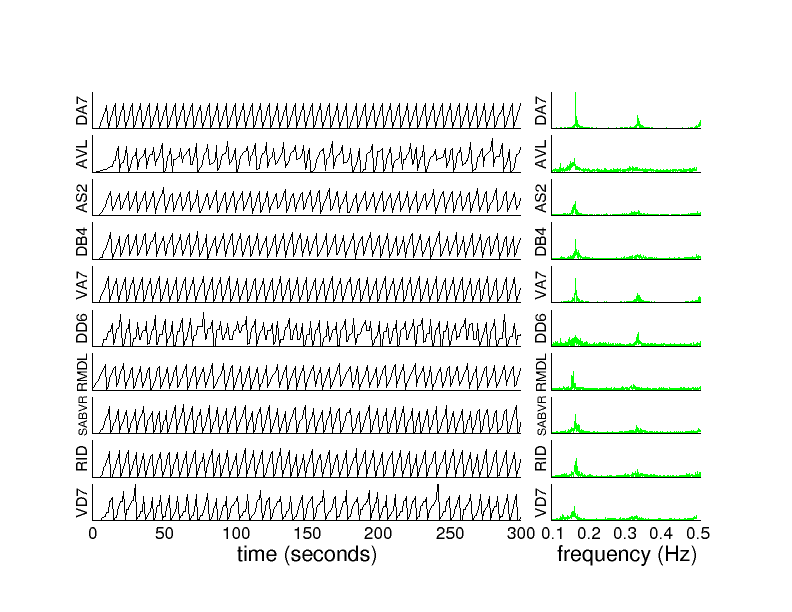
\includegraphics[width=\imsize]{cluster1.png}
	\caption[ Señales de todas las neuronas del grupo sincronizado $\Omega_1$ en un intervalo de cinco minutos, y sus transformadas de Fourier correspondientes en un experimento de 20 minutos de duración.]{Señales de todas las neuronas del grupo sincronizado $\Omega_1$ en un intervalo de cinco minutos, y sus transformadas de Fourier correspondientes en un experimento de 20 minutos de duración.}\label{fig:cluster_1}
\end{figure}
 \begin{figure}[h!]
	\centering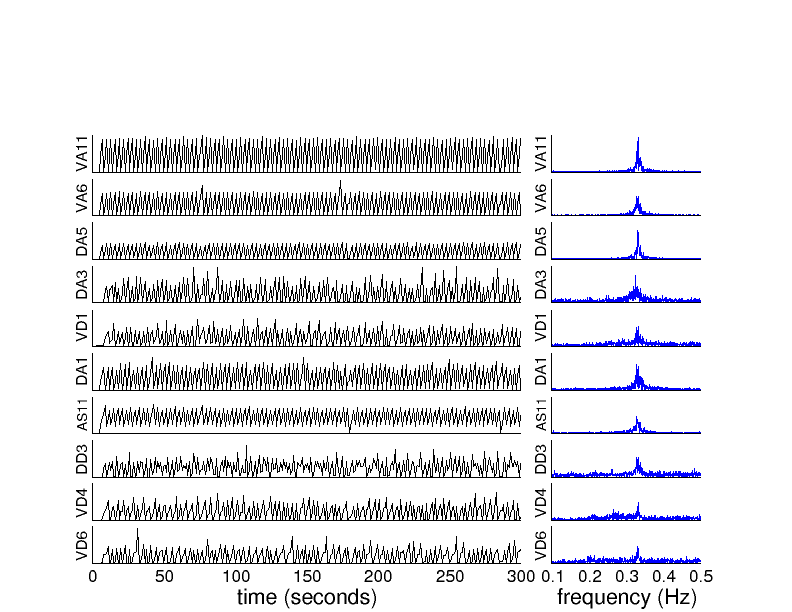
\includegraphics[width=\imsize]{cluster_2.png}
	\caption[ Señales de todas las neuronas del grupo sincronizado $\Omega_2$ en un intervalo de cinco minutos, y sus transformadas de Fourier correspondientes en un experimento de 20 minutos de duración.]{Señales de todas las neuronas del grupo sincronizado $\Omega_1$ en un intervalo de cinco minutos, y sus transformadas de Fourier correspondientes en un experimento de 20 minutos de duración.}\label{fig:cluster_2}
\end{figure}
 \begin{figure}[h!]
	\centering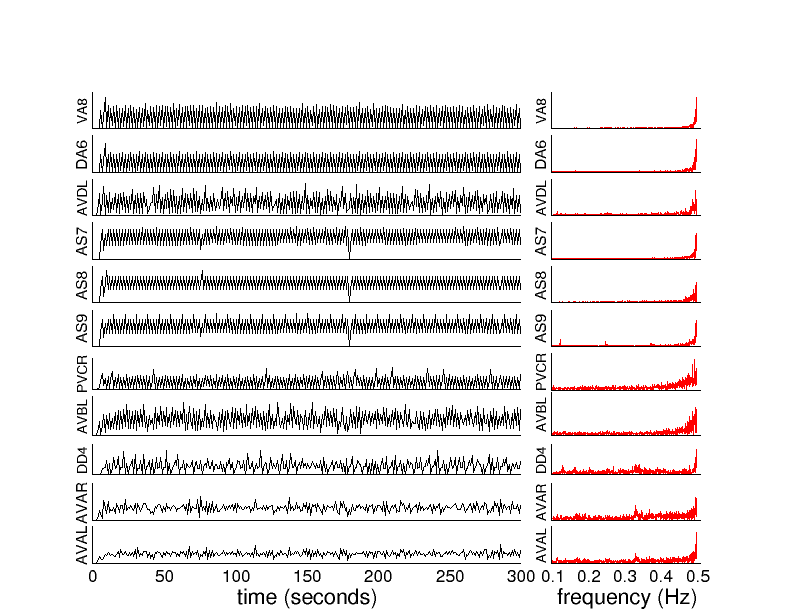
\includegraphics[width=\imsize]{cluster_3.png}
	\caption[ Señales de todas las neuronas del grupo sincronizado $\Omega_3$ en un intervalo de cinco minutos, y sus transformadas de Fourier correspondientes en un experimento de 20 minutos de duración.]{Señales de todas las neuronas del grupo sincronizado $\Omega_1$ en un intervalo de cinco minutos, y sus transformadas de Fourier correspondientes en un experimento de 20 minutos de duración.}\label{fig:cluster_3}
\end{figure}

La \Cref{fig:sincronia_2}B se asemeja mucho a la formación de grupos sincronizados en osciladores Kuramoto con una amplia distribución de frecuencias naturales \cite{manrubia_emergence_2004}.  Sin embargo, en este caso, los nodos tienen una dinámica idéntica, ya que todas las neuronas tienen el mismo umbral de disparo, y la heterogeneidad surge de la compleja red de interacciones dada por el conectoma de C. elegans. Una comparación directa de la lista de entradas sensoriales y salidas cinéticas con las neuronas de los grupos sincronizados revela que no es un efecto trivial de la estimulación directa (Ver la \Cref{sec:dinamica} para ver las neuronas estimuladas).  Como se discutió en el \Cref{sec:aleaotrioconectoma} para probar que la emergencia de grupos sincronizados no es un epifenómeno, analizamos la dinámica en versiones aleatorizadas del conectoma donde se conservan la distribución de grados y las distribuciones de pesos. Es decir, las redes aleatorias tienen exactamente la misma distribución de grados de entrada y salida y distribuciones de pesos asignadas aleatoriamente a los nodos y enlaces. En todos los casos, encontramos que las acciones emergentes del robot se pierden (ver video suplementario S2) y no se observan grupos sincronizados (ver \Cref{fig:sincronia_2}C).

Como se discutió anteriormente Kato et al. \cite{kato_global_2015} utilizaron técnicas de imagen de calcio para registrar la actividad neuronal con resolución de célula única en todos los ganglios cefálicos y algunas neuronas motoras del cordón ventral. En estos experimentos, se escanearon $\sim$100 neuronas tres veces por segundo durante periodos de 20 minutos, generando conjuntos de datos de alta dimensión. Utilizando el análisis de componentes principales (PCA) para la reducción de dimensionalidad, pudieron agrupar neuronas con señales correlacionadas. En particular, produjeron vectores de pesos neuronales (PC), mostrando que los grupos con signos opuestos en sus PC oscilan en antifase, y que de acuerdo con el signo de su vector de pesos se correlacionan con el comportamiento hacia adelante o hacia atrás del gusano.   Siguiendo el mismo procedimiento, también realizamos un análisis de componentes principales similar. Al igual que en Kato et al., cada una de las series temporales neuronales se normalizó utilizando el valor medio ($\bar{s}$) y la desviación estándar ($\sigma_s$):

\begin{equation}
s^{\prime}(t)=\frac{s(t)-\bar{s}(t)}{\sigma_s(t)}
\end{equation}


de modo que las nuevas series temporales tienen ahora media cero y desviación estándar unitaria. A continuación, se calcularon los componentes principales en función de la estructura de covarianza de los datos normalizados, produciendo vectores de pesos neuronales (PC) para las series temporales neuronales de todas las neuronas del robot. Esto nos permitió avanzar en la caracterización cuantitativa de los grupos sincronizados en frecuencia.  En la \Cref{fig:sincronia_3} (arriba) representamos las frecuencias características de los tres grupos sincronizados en frecuencia $\Omega_1$ (verde), $\Omega_2$ (azul) y $\Omega_3$ (rojo) ya presentados en la \Cref{fig:sincronia_2}. Las neuronas se han ordenado ahora en función de su primer peso de componente principal (PC1; \Cref{fig:sincronia_3} (abajo)), es decir, las neuronas de la izquierda tienen el valor positivo más alto, mientras que las de la derecha tienen el valor negativo más bajo de PC1. Obsérvese que todos los grupos sincronizados implican neuronas con valores de PC1 tanto positivos como negativos. El grupo con menor frecuencia, $\omega_1$, presenta una amplia distribución de pesos neuronales. Para frecuencias más altas, las neuronas presentan una mayor segregación hacia valores extremos de PC1. De hecho, tanto $\Omega_2$ como $\Omega_3$ están claramente divididos en dos subgrupos más pequeños: uno con solo valores positivos de PC1 y otro con solo valores negativos de PC1. Esta segregación refleja diferencias en los tiempos de disparo de las neuronas. En cada grupo, los tiempos de disparo de las neuronas son proximales. En cambio, cuando se comparan las señales de las neuronas entre grupos, se observa un desplazamiento en su fase relativa. El mayor desplazamiento se produce para valores extremos de PC, cuando las neuronas de los diferentes subgrupos de la misma frecuencia oscilan principalmente en antifase (véase la \Cref{fig:antifase}).

 \begin{figure}[h!]
	\centering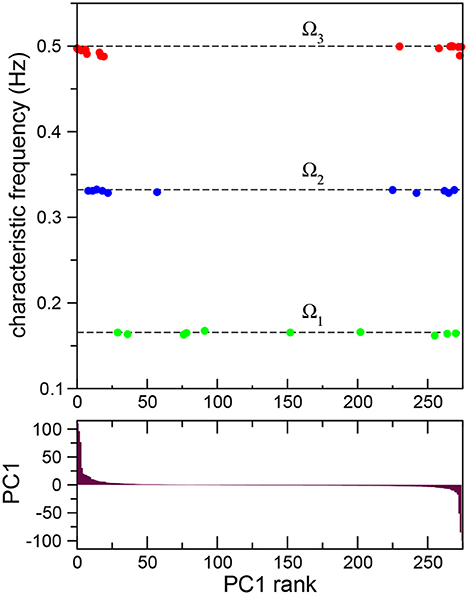
\includegraphics[width=\imsize]{sincronia3.jpg}
	\caption[ Sincronización de frecuencias ordenada según el análisis de componentes principales.]{Sincronización de frecuencias ordenada según el análisis de componentes principales. Transformadas de Fourier promedio de las neuronas de tres grupos sincronizados en frecuencia (arriba) para un experimento completo de 15 minutos de duración ordenadas según su primer componente principal PC1 (abajo). El análisis revela la presencia de subgrupos con signos opuestos en su peso de componente principal.}\label{fig:sincronia_3}
\end{figure}

 \begin{figure}[h!]
	\centering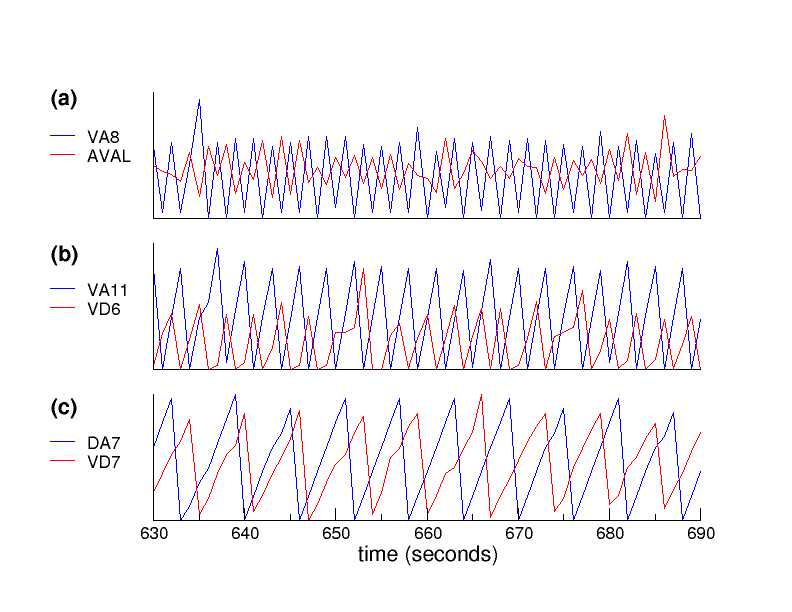
\includegraphics[width=\imsize]{antifase.png}
	\caption[ Sincronización de frecuencias ordenada según el análisis de componentes principales.]{Oscilaciones en antifase de las neuronas con el mayor PC1 positivo (azul) y el menor PC1 negativo (rojo). (a) VA8 y AVAL en el grupo $\Omega_3$, (b) VA11 y VD6 en el grupo $\Omega_2$, y (c) DA7 y VD7 en el grupo $\Omega_1$. Todas las figuras se presentan en el mismo intervalo de tiempo de 60 segundos.}\label{fig:antifase}
\end{figure}

\subsection{Dinámica neuronal anidada}

Ahora analizamos cómo las oscilaciones colectivas en los grupos sincronizados en frecuencia también están acopladas entre sí. En la \Cref{fig:sincronia_2}A mostramos las transformadas de Fourier promedio de las neuronas en tres grupos sincronizados en frecuencia. Obsérvese que la TF promedio del grupo con la frecuencia más baja, $\Omega_1$, también tiene dos picos más pequeños, que coinciden con la frecuencia característica de los otros grupos: $\Omega_2$ y $\Omega_3$. Como guía para el ojo, indicamos con líneas discontinuas estas frecuencias en los tres paneles. Esto revela un acoplamiento entre los diferentes grupos sincronizados en frecuencia.

Para estudiar cuantitativamente el acoplamiento entre oscilaciones a diferentes frecuencias, analizamos las señales de las neuronas de un grupo dado cuando la señal de una neurona de otro grupo con una frecuencia característica más baja alcanza su máximo \cite{jensen_cross-frequency_2007}.   Si hay un acoplamiento entre las oscilaciones, entonces esperamos que la señal de la neurona con mayor frecuencia pueda presentar pequeñas fluctuaciones alrededor del mismo valor medio cada vez que se alcanza el máximo con la frecuencia más baja. Por el contrario, si no hay acoplamiento, se espera que la señal varíe aleatoriamente. En la \Cref{fig:anidado} representamos las señales de las neuronas de $\Omega_2$ y $\Omega_3$ cuando una neurona seleccionada del grupo con menor frecuencia característica $\Omega_1$ alcanza su máximo. En particular, nos centramos en las neuronas con el mayor peso de PC1 positivo en cada uno de los grupos sincronizados. Las Figuras \Cref{fig:anidado}A, B muestran que estas neuronas están acopladas, ya que el mismo valor medio persiste en intervalos de tiempo prolongados. Además, para visualizar este resultado, representamos en la \Cref{fig:anidado}E las señales de estas neuronas en un intervalo de tiempo fijo, utilizando líneas verticales discontinuas como guía para el ojo. La figura muestra claramente una relación jerárquica anidada entre oscilaciones a diferentes frecuencias. En las \Cref{fig:anidado}C, D representamos las señales de las neuronas que tienen los pesos de PC1 negativos más bajos. En marcado contraste con las neuronas con pesos positivos, las señales no están correlacionadas y fluctúan a lo largo de todo el experimento.


 \begin{figure}[h!]
	\centering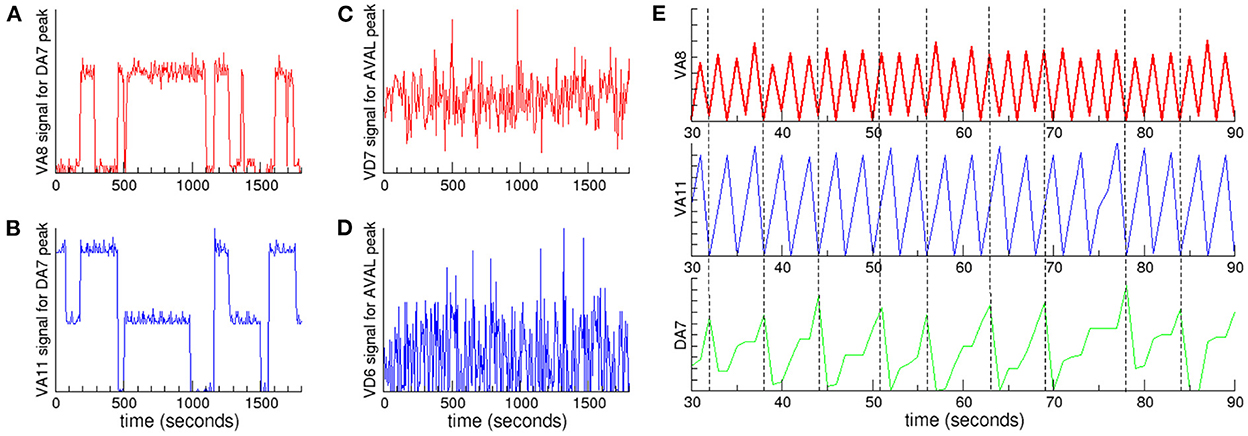
\includegraphics[width=\imsize]{anidado.jpg}
	\caption[ Dinámica neuronal anidada.]{Dinámica neuronal anidada. Representamos las señales de las neuronas de los grupos $\Omega_2$ y $\Omega_3$ cuando una neurona seleccionada del grupo $\Omega_1$ alcanza su máximo: (A) señal de VA8 (roja) del grupo $\Omega_3$ y (B) VA11 (azul) del grupo $\Omega_2$, cuando DA7 del grupo $\Omega_1$ alcanza su máximo. El acoplamiento entre las neuronas de estos grupos aparece como regiones caracterizadas por señales con pequeñas fluctuaciones alrededor de un valor medio. En cambio, cuando no hay acoplamiento las señales presentan grandes fluctuaciones, como se muestra por ejemplo para las señales de (C) VD7 (roja) del grupo $\Omega_3$ y (D) VD6 (azul) del grupo $\Omega_2$, cuando AVAL del grupo $\Omega_1$ alcanza su máximo. (E) Un intervalo de tiempo de 60 segundos de los datos presentados en (A, B) muestra la relación jerárquica. Las señales corresponden a VA8 (roja), VA11 (azul) y DA7 (verde). Las líneas verticales discontinuas son una guía para el ojo que muestran el momento en que DA7 alcanza su máximo.}\label{fig:anidado}
\end{figure}

\subsection{Dinámica neuronal y acciones del robot}

En esta sección analizamos la correlación entre la dinámica neuronal emergente y las acciones del robot. El modelo robótico es muy adecuado para este estudio, ya que permite registrar la dinámica neuronal mientras se registran simultáneamente las acciones. Para determinar si había una correlación entre una acción determinada y la actividad de neuronas específicas, contrastamos las series temporales de la dinámica neuronal con las series temporales de las acciones del robot. En primer lugar, registramos todos los eventos de acción en un experimento de 20 minutos de duración. A continuación, analizamos qué acciones estaba ejecutando el robot cuando una neurona determinada se había activado, es decir, cuando su valor se restablecía a cero. Por último, contrastamos las fracciones de eventos de estas dos series temporales para ver si había variaciones significativas.

En los experimentos, el robot se mueve principalmente hacia adelante y hacia atrás, mientras que los giros suelen ser eventos cortos en los que el robot solo cambia de dirección, por lo que nos centramos principalmente en los eventos de avance y retroceso. Estos eventos corresponden a la respuesta de la red a la estimulación de las neuronas sensoriales \footnote{\url{https://wormatlas.org/hermaphrodite/nervous/Images/neurotable1leg.htm}}.  Como se discutió en el \Cref{sec:estimuladas}  tal como se observa en el gusano, la estimulación de las neuronas de quimiotaxis promueve el desplazamiento sostenido y hace que el robot se mueva hacia adelante, mientras que la estimulación de las neuronas sensoriales que promueven la evitación hace que el robot se mueva hacia atrás. En este punto, cabe destacar que estas respuestas de acción son emergentes y no triviales, en el sentido de que solo se estimula una pequeña fracción de todas las unidades dinámicas, y por lo tanto las respuestas corresponden a una modulación de la dinámica global.


Encontramos que las neuronas de los grupos sincronizados con los mayores pesos de PC1 positivos promueven eventos de avance, mientras que las neuronas con los pesos negativos más bajos promueven eventos de retroceso. La \Cref{fig:neuronas_comportamiento} muestra la fracción de eventos registrados cuando se disparan las neuronas con los mayores pesos de PC1 positivos y negativos en los grupos sincronizados (véase también el \Cref{table:neuronas_comportamiento}). Las barras de color corresponden a: $\Omega_1$ (verde), $\Omega_2$ (azul) y $\Omega_3$ (rojo). En cada figura, los resultados se contrastan con las fracciones de eventos para todo el experimento (barras grises). Obsérvese que se observa un aumento significativo de los eventos de avance cuando se disparan las neuronas con el mayor PC1 positivo (primeras columnas de las \Cref{fig:neuronas_comportamiento}A, C, E), mientras que se observa una reducción en las neuronas con el menor PC1 negativo (primeras columnas de las \Cref{fig:neuronas_comportamiento}B, D, F). Al mismo tiempo, se observa un aumento de los eventos de retroceso cuando se disparan neuronas con PC negativas (columnas discontinuas de las \Cref{fig:neuronas_comportamiento}B, D, F), mientras que se observa una disminución de la fracción de eventos de retroceso en las neuronas con pesos positivos (columnas discontinuas de las \Cref{fig:neuronas_comportamiento}A, C, E). Estos resultados revelan el papel que juega la segregación de las neuronas en los grupos sincronizados en la promoción de diferentes acciones que el robot ejecuta. Es interesante que, en C. elegans, Kato et al. \cite{kato_global_2015} observaron que las neuronas que promueven comportamientos opuestos, como el avance y el retroceso, también tienen signos opuestos en sus pesos de PC1.

 \begin{figure}[h!]
	\centering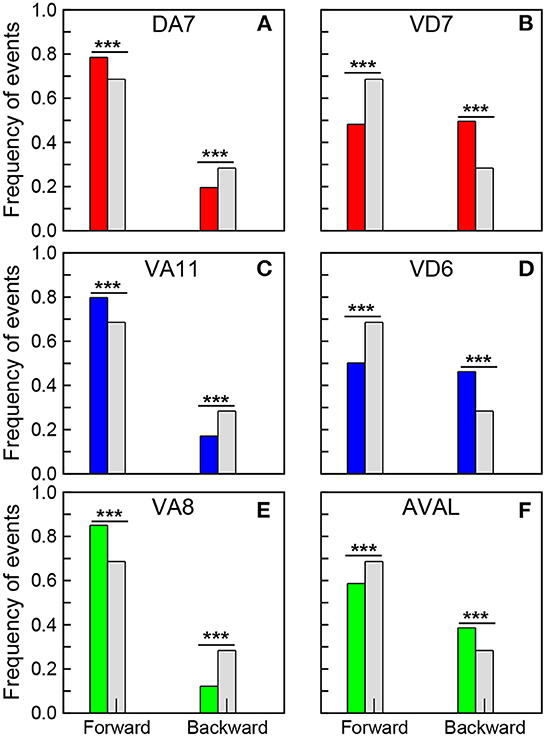
\includegraphics[width=\imsize]{neuronas_comportamiento.jpg}
	\caption[ Correlación de la dinámica neuronal con las acciones del robot.]{Correlación de la dinámica neuronal con las acciones del robot. Fracción de eventos de avance y retroceso registrados cuando las neuronas seleccionadas dispararon. (A) DA7, (C) VA11 y (E) VA8 corresponden a las neuronas con el mayor PC1 positivo en los grupos sincronizados $\Omega_1, \Omega_2$ y $\Omega_3$, mientras que (B) VD7, (D) VD6 y (F) AVAL corresponden a las neuronas con el PC1 negativo más bajo en estos grupos. Las barras grises corresponden a la fracción de eventos de avance y retroceso en un experimento de 20 minutos de duración. Una prueba de chi-cuadrado (estadísticamente significativa, $***p-value < 0.00001$) muestra que los efectos opuestos de todas estas neuronas en las acciones del robot son significativos.}\label{fig:neuronas_comportamiento}
\end{figure}


\begin{table}[h!]
	\centering
	\caption[Fracción de eventos hacia adelante y hacia atrás registrados cuando las neuronas correspondientes se dispararon.  ]{ Fracción de eventos hacia adelante y hacia atrás registrados cuando las neuronas correspondientes se dispararon.   La fracción de eventos para todo el experimento de 20 minutos fue Adelante = 0.69 y Atrás = 0.28.}
	\begin{tblr}{colspec={lll},
			row{odd} = {bg=gray8},
			row{even} = {bg=gray9},
			row{1} = {bg=red3, fg=white, font=\sffamily},
		}
		
Neurona & 	Adelante &	Atrás\\
DA7 &	0.79 &	0.20\\
VD7	& 0.48 &	0.50\\
VA11 &	0.80 &	0.17\\
VD6	& 0.50&	0.46\\
VA8	& 0.85 &	0.12\\
AVAL&	0.59&	0.39
		
	\end{tblr}
	\label{table:neuronas_comportamiento}
\end{table}

\subsection{Discusión}

Sorprendentemente, también observamos la emergencia de una estructura jerárquica anidada. En el gusano, Kaplan et al. \cite{kaplan_nested_2020} mostraron que la presencia de una estructura jerárquica en la dinámica neural permite la coordinación de comportamientos a través de diferentes escalas de tiempo. Esto incluye los movimientos de la cabeza, las ondulaciones del cuerpo y también los episodios de avance y retroceso. Vale la pena recalcar que el diseño simple del robot que utilizamos no permite la ejecución de algunos de estos comportamientos. Sin embargo, Kaplan et al. \cite{kaplan_nested_2020} observaron que la estructura jerárquica persistía incluso cuando los animales estaban inmovilizados, concluyendo que es una propiedad intrínseca que emerge de las neuronas y sus interacciones en los circuitos. Los resultados obtenidos con el robot destacan esta conclusión, es decir, que la presencia de una dinámica anidada es una propiedad emergente de las interacciones de las neuronas a través del conectoma.



\section{Discusión}

El nematodo C. elegans ha sido un organismo modelo de elección en la investigación neurocientífica debido a su capacidad para ofrecer una visión integrada de cómo el sistema nervioso, el cuerpo y el entorno interactúan como un sistema dinámico acoplado. Dos estudios destacados de Kato et al. \cite{kato_global_2015} y Kaplan et al. \cite{kaplan_nested_2020} han demostrado que el comportamiento de C. elegans se encuentra codificado en una jerarquía de dinámicas neuronales de baja dimensión. Estos hallazgos respaldan la hipótesis de que los estados de comportamiento emergen de la interacción neuronal y de circuitos complejos.

En este contexto, hemos aplicado un modelo robótico basado en el conectoma de C. elegans para explorar y poner a prueba estas ideas. No buscábamos replicar al gusano exactamente, sino construir robots inspirados en la conceptualización de Busbice. La elección se basó en el diseño simplificado de estos robots, que permite un enfoque de sistema complejo. A través de esta aproximación, hemos observado diversas características emergentes que también se manifiestan en C. elegans, incluyendo la formación de grupos sincronizados de actividad neuronal correlacionados con acciones.

Nuestros experimentos han revelado que el robot a menudo muestra comportamientos coherentes con las observaciones en C. Elegans. Esto sugiere que la integración de un conectoma en una entidad mecánica abre un abanico de oportunidades para futuras investigaciones. A medida que continuamos refinando nuestra capacidad para emular la dinámica neuronal, y para modelar una neurona con mayor precisión dentro de un conectoma completo, la exploración de los sistemas nerviosos se torna más accesible y ética en comparación con la experimentación con animales.

Nuestros hallazgos respaldan la idea de que la estructura de red del conectoma de C. elegans es fundamental para su dinámica neuronal. Estos resultados podrían extenderse a otros conectomas, ya que hemos identificado principios comunes en la organización de sistemas nerviosos en diferentes especies \cite{heuvel_comparative_2016}. Al mismo tiempo, las diferencias en los resultados pueden proporcionar insights valiosos sobre las adaptaciones específicas de cada especie.

A medida que avanzamos hacia redes neuronales de mayor envergadura y detalle, nos enfrentamos a nuevos desafíos relacionados con la complejidad y la alta dimensionalidad de los datos. El conectoma del hemicerebro de Drosophila, que involucra un gran número de neuronas \cite{scheffer_connectome_2020}, ejemplifica esta complejidad. Nuestro modelo robótico simple, sin embargo, proporciona una herramienta útil para probar hipótesis relacionadas con la estructura y la función del sistema nervioso.

Además, la implementación de conectomas funcionales en robots podría impulsar la investigación en robótica autónoma. Por ejemplo, la capacidad de emular a un organismo en la búsqueda de comida o la detección de sobrevivientes en un edificio derrumbado podría tener aplicaciones en situaciones de desastre. La extensión de este enfoque a otros conectomas de nivel superior, como los de peces, drosófilas y ratones, promete expandir significativamente nuestro conocimiento en neurociencia.

En la segunda parte de nuestra investigación, nos adentramos en el apasionante campo de la hipótesis de criticidad neuronal. Esta hipótesis postula que los organismos están optimizados para operar en el punto crítico, que es un estado intermedio entre el caos y el orden. Similar a las transiciones de fase en la física, en este estado, los organismos pueden realizar comportamientos complejos y adaptarse a su entorno de manera eficiente. Hasta el momento, la literatura científica carecía de estudios que investigaran si un organismo tan pequeño como C. elegans muestra signos de comportamientos complejos relacionados con la criticidad neuronal.

La próxima fase de nuestra tesis busca abordar esta pregunta fundamental: ¿Existen indicios de criticidad neuronal en C. elegans? Para responder a esta pregunta, realizaremos un análisis detallado utilizando datos experimentales de C. elegans reales y un modelo basado en el trabajo de Haimovici et al. Estos esfuerzos llenarán un vacío en la investigación y arrojarán luz sobre si C. elegans opera en un estado de criticidad neuronal, lo que tendría implicaciones significativas para nuestra comprensión de la biología y la neurociencia.
































\part{Modelado, Validación Experimental y Criticalidad Neuronal en C. elegans}\label{sec:parteII}

\chapter{Dinámica neuronal critica}\label{titulo-cap-critico}
\graphicspath{{figs/capitulo_critico/}}

\chapterquote{Can a machine be made to be supercritical? }{Alan Turing , 1950}






\section{Introducción}

La física de sistemas complejos ha demostrado que los comportamientos colectivos pueden surgir de la interacción entre los constituyentes elementales de la materia, dando lugar a fases con diferentes niveles de orden interno. Los sistemas biológicos no son la excepción, y algunos de ellos han sido identificados como operando en la vecindad del punto crítico de una transición de fase. En este sentido, la hipótesis de la criticidad neuronal sugiere que el cerebro puede estar en un estado crítico en el límite entre diferentes tipos de dinámicas, lo que le proporcionaría un equilibrio óptimo entre robustez y flexibilidad.

En este capítulo se revisarán las bases teóricas de la física de sistemas complejos y su aplicación en biología, así como los fundamentos de la hipótesis de la criticidad neuronal y las evidencias experimentales que la respaldan.






\section{Física de sistemas complejos y transiciones de fase}

\subsection{Transiciones de fase en física}

La materia, compuesta por átomos, moléculas y electrones, puede generar diversas fases cuyo comportamiento difiere significativamente de sus componentes individuales o pequeños grupos de ellos. A nivel microscópico, los sistemas que contienen muchos componentes pueden exhibir diferentes tipos de comportamientos colectivos a nivel macroscópico, es decir, fases, con diferentes niveles de orden interno. Es importante destacar que incluso pequeños cambios en las condiciones externas, como la temperatura o la presión, pueden inducir reordenamientos estructurales drásticos, lo que se conoce como transiciones de fase.\\

En la distinción de las distintas fases de un sistema, se consideran ciertas propiedades macroscópicas medibles, conocidas como parámetros de orden. La variación de una propiedad ambiental, denominada parámetro de control, permite observar cómo dichos parámetros de orden cambian. En general, una modificación gradual en el parámetro de control se traduce en una alteración suave en los parámetros de orden. Sin embargo, existen determinados puntos donde los valores de los parámetros de orden experimentan saltos o giros abruptos (ver \Cref{fig:trancisiones}). Estos puntos marcan los límites entre diferentes fases, y desplazar el parámetro de control a través de dicho límite induce una transición de fase.\\

En función de cómo se modifiquen los parámetros de orden durante una transición de fase, esta puede ser de dos tipos. Si la transición se caracteriza por un salto en los parámetros de orden del sistema, lo que matemáticamente corresponde a una discontinuidad en el diagrama de fase, se trata de una transición de fase discontinua (ver \Cref{fig:transicionI} ). Este tipo de transiciones son denominadas a veces como transiciones de primer orden. Por otra parte, si el diagrama de fase es continuo y la transición se caracteriza por una esquina aguda (es decir, un punto de no diferenciabilidad), se trata de una transición de fase continua (segundo orden, ver \Cref{fig:transicionII}). La terminología de \textquote{primer orden} y \textquote{segundo orden} se origina en la descripción de las transiciones de fase termodinámicas, haciendo referencia a la derivada más baja de la energía libre, la cual muestra una discontinuidad en el punto crítico.\\


\begin{figure}[ht]
	\centering
	\begin{subfigure}[b]{0.45\textwidth}
		\centering
		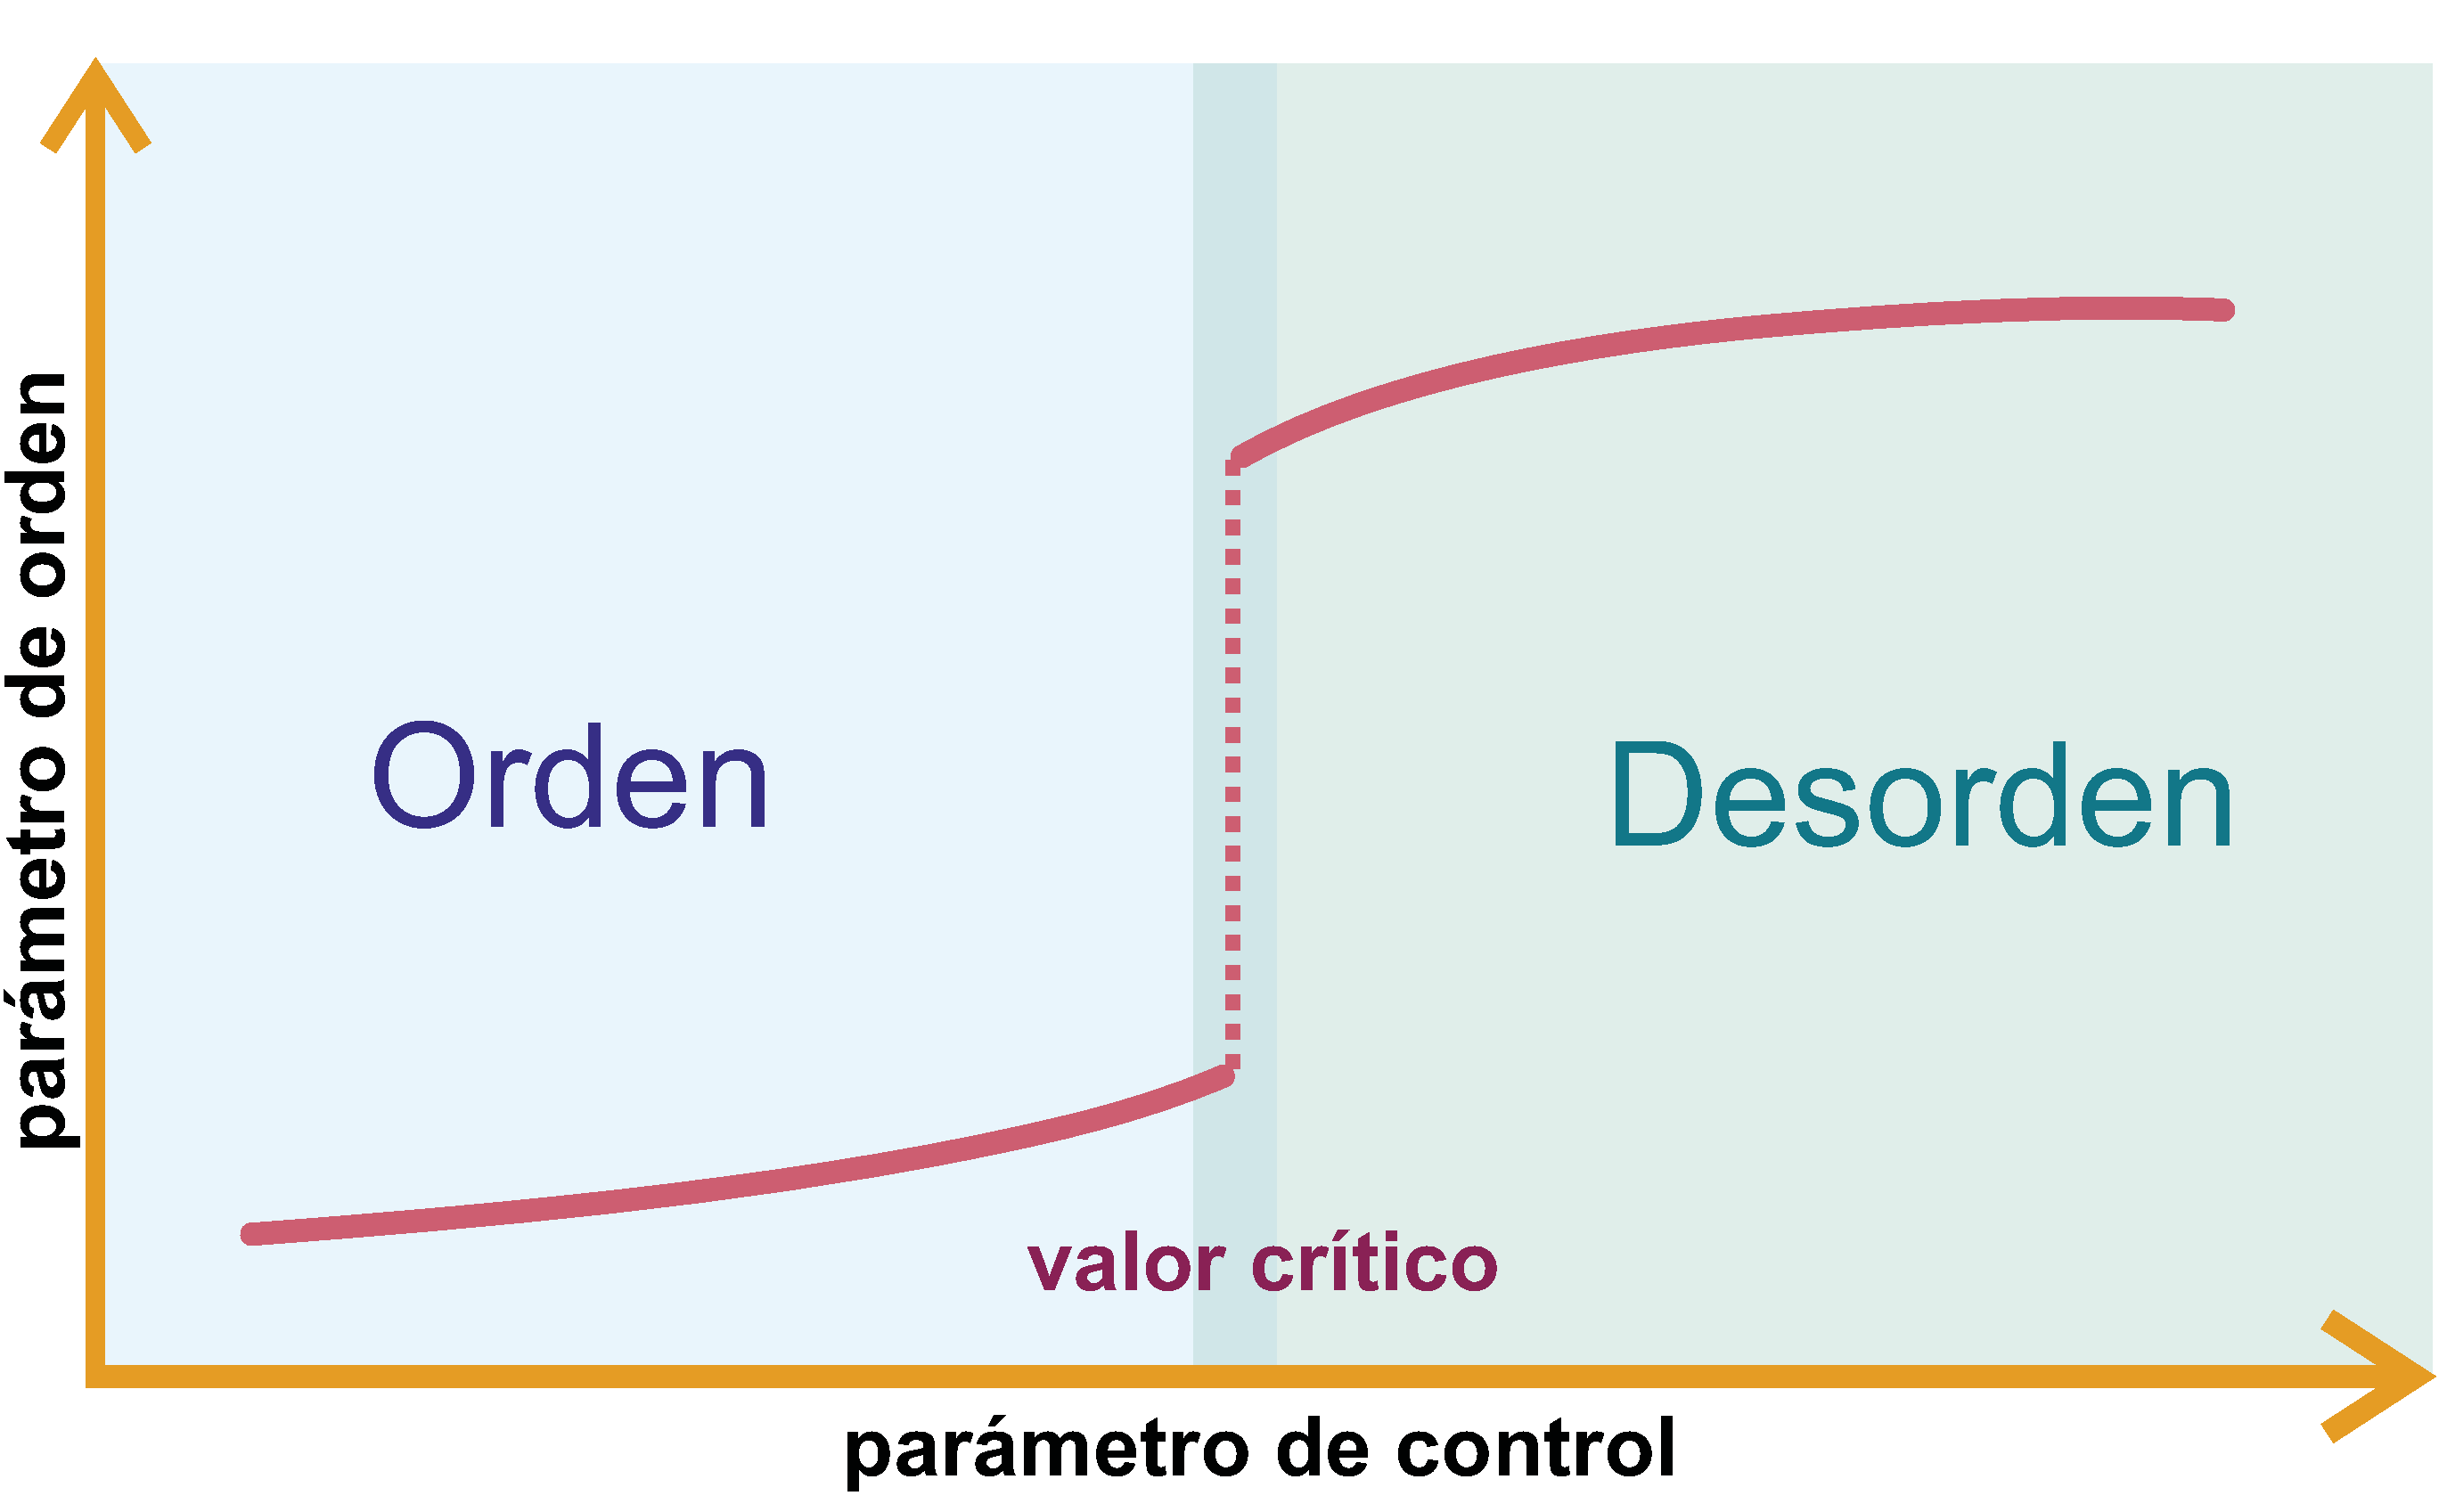
\includegraphics[width=\textwidth]{transiciones_fases_tipo_I.pdf}
		%\caption{transiciones de fase de primer orden}
		\caption{}
		\label{fig:transicionI}
	\end{subfigure}
	\begin{subfigure}[b]{0.45\textwidth}
		\centering
		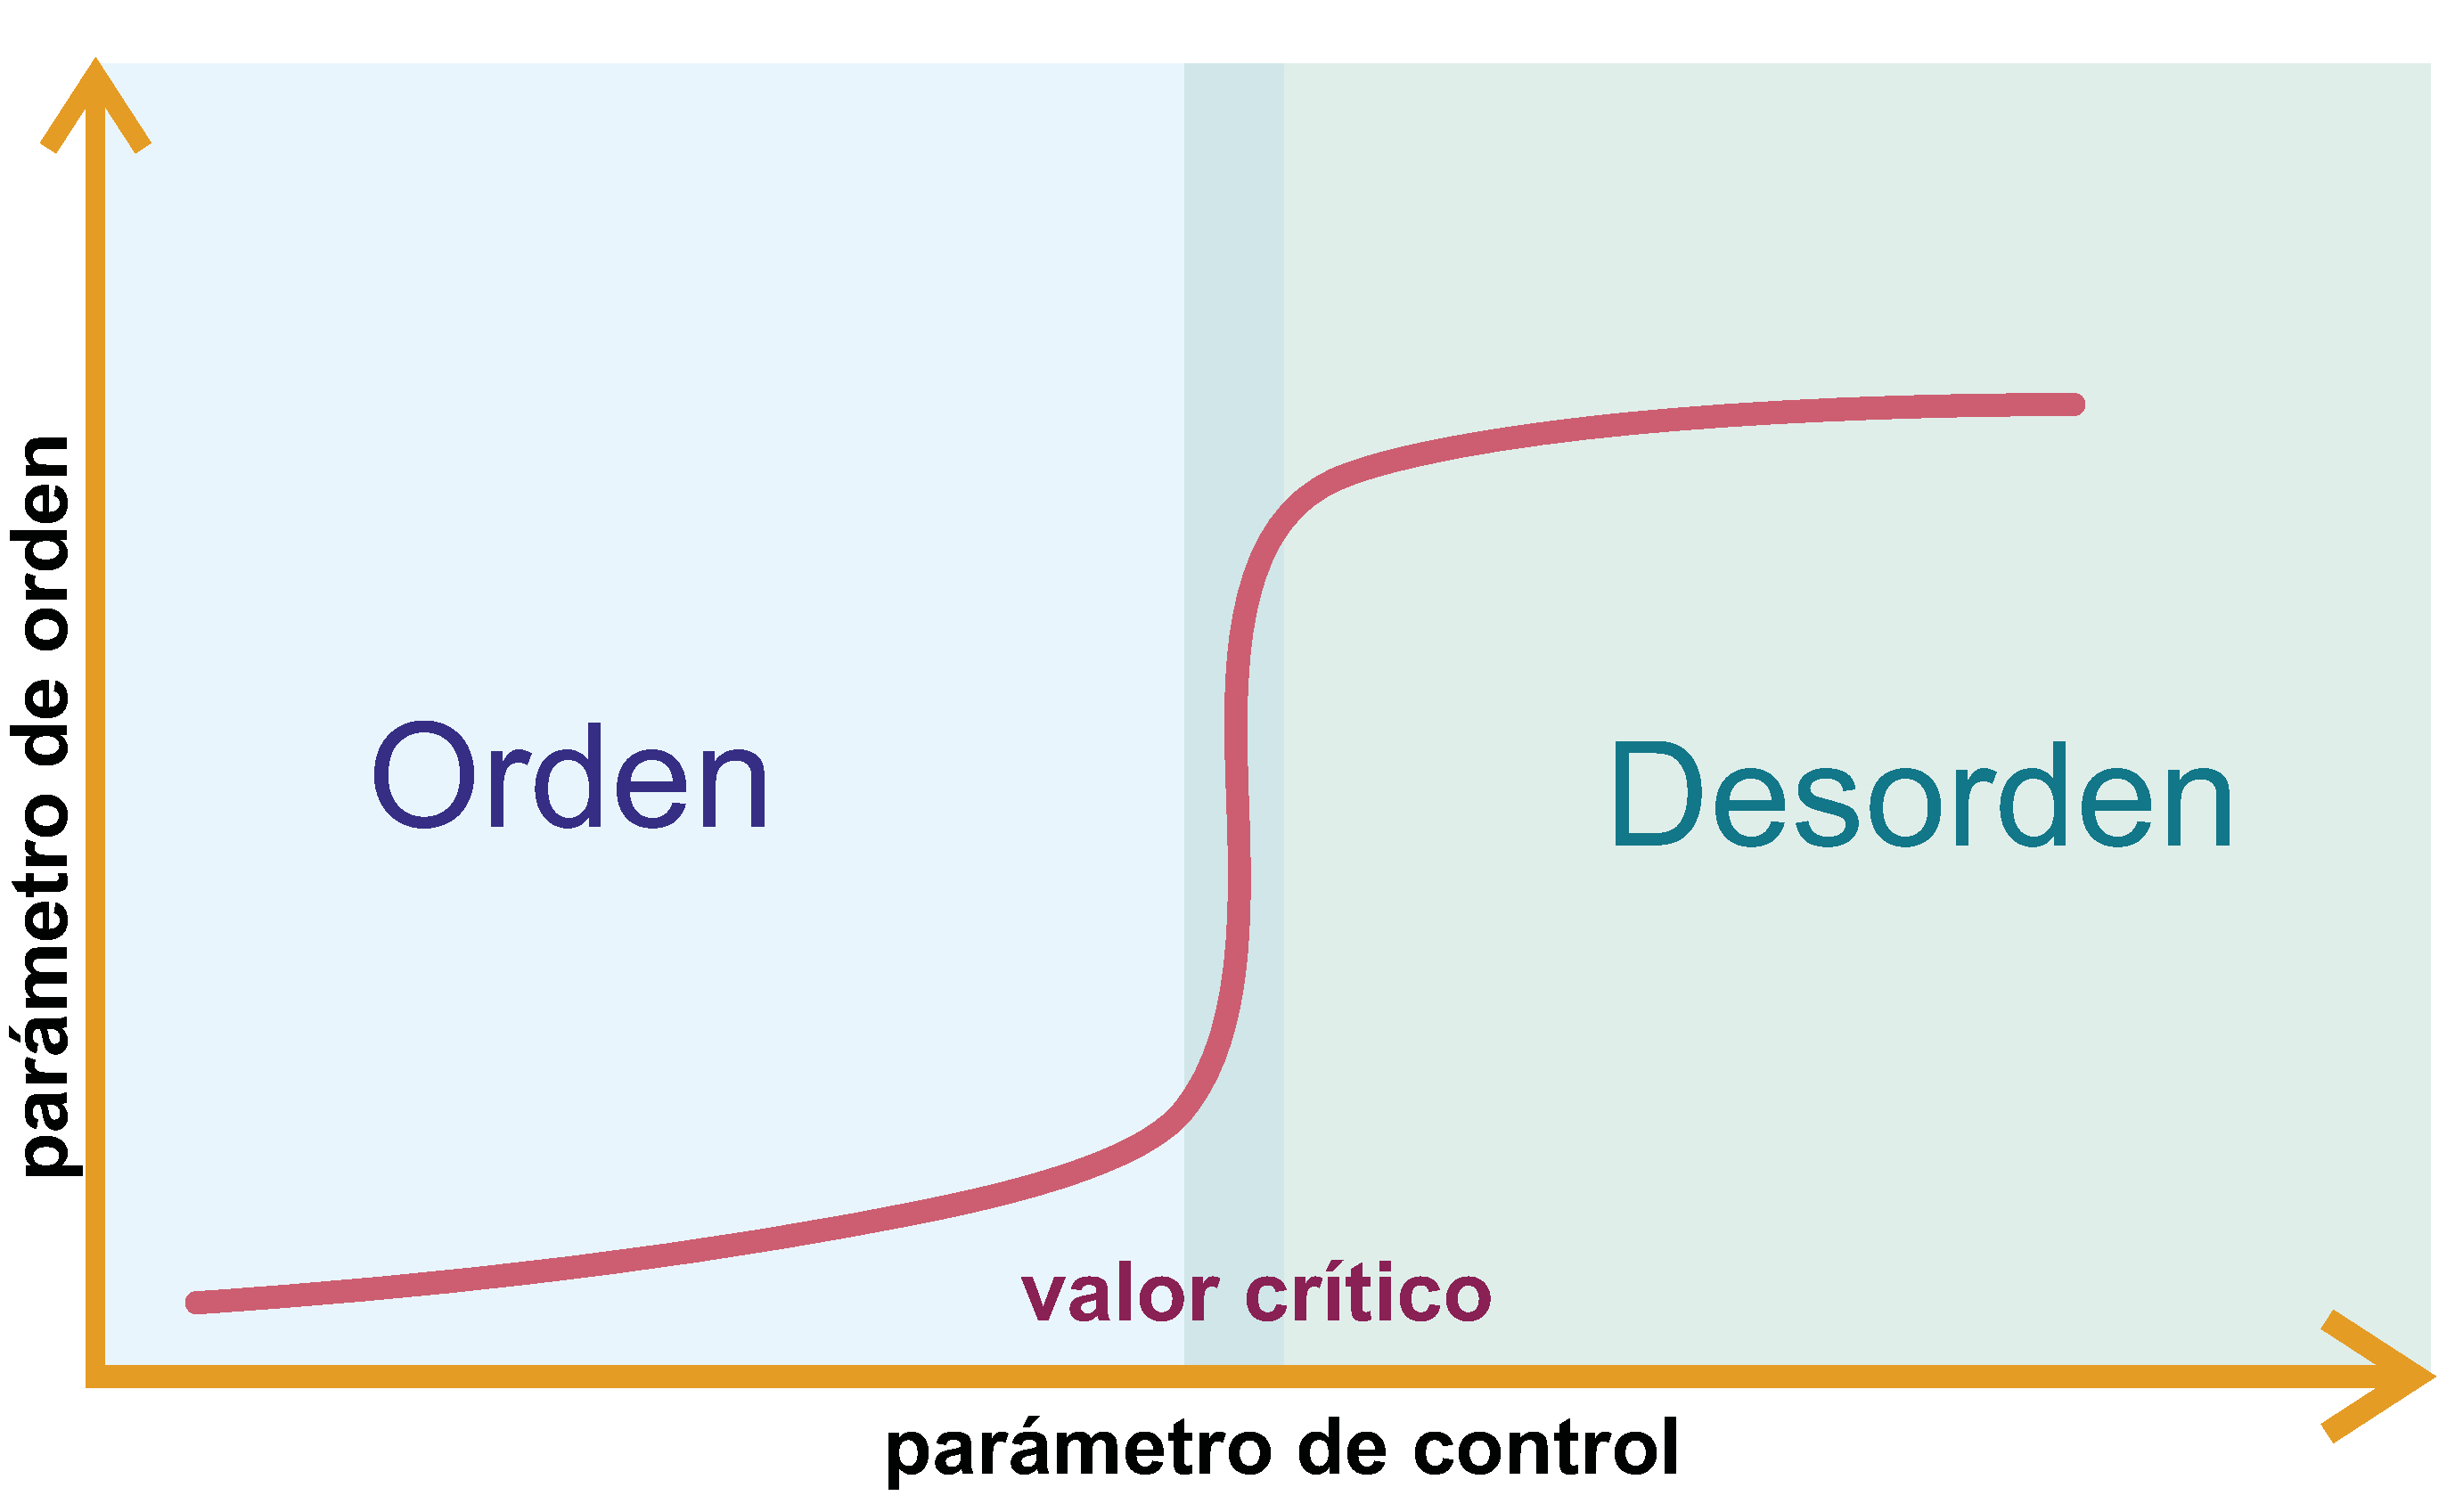
\includegraphics[width=\textwidth]{transiciones_fases_tipo_II.pdf}
		%\caption{transiciones de fase de segundo orden}
		\caption{}
		\label{fig:transicionII}
	\end{subfigure}
	\caption[Representaciones esquemáticas de transiciones de fase de primer y segundo orden.]{Representaciones esquemáticas de transiciones de fase de primer y segundo orden. La figura muestra dos ejemplos de transiciones de fase que ocurren en sistemas termodinámicos. En (a), se ilustra una transición de fase de primer orden, donde el parámetro de orden experimenta un cambio abrupto en su valor crítico del parámetro de control. En contraste, en (b) se muestra una transición de fase de segundo orden, donde el parámetro de orden varía suavemente a medida que cambia el parámetro de control.}
	\label{fig:trancisiones}
\end{figure}

Si un sistema exhibe una transición de fase continua, entonces puede existir en un punto crítico que se encuentra exactamente en la frontera entre dos fases distintas. Este estado límite, conocido como estado crítico, se caracteriza por la presencia de fluctuaciones importantes en el valor del parámetro de orden en el rango crítico, lo cual refleja la pérdida de simetría del sistema que ocurre durante las transiciones de fase. Por consiguiente, se considera que los estados críticos se encuentran en la frontera del caos. Las transiciones de fase críticas son especialmente interesantes debido al comportamiento crítico que se manifiesta en las grandes fluctuaciones del parámetro de orden, las cuales exhiben escalamiento de ley de potencia (Figura 1C).\\



\subsection{Transiciones de fase en biología}


El principio de universalidad es un concepto ampliamente aceptado en la física que establece que las características relevantes de los fenómenos a gran escala son altamente insensibles a los detalles específicos del modelo y se comparten entre sistemas aparentemente distintos. Siguiendo este principio, se ha propuesto una hipótesis controvertida, pero ampliamente investigada, según la cual algunos sistemas biológicos pueden obtener beneficios funcionales significativos al operar cerca del punto crítico de una transición de fase \cite{munoz_colloquium_2018,hidalgo_information-based_2014,kauffman_origins_1993,bak_how_1996,chialvo_brain_2008,chialvo_emergent_2010,plenz_critical_2013,niebur_criticality_2014,shew_functional_2013,cocchi_criticality_2017,zimmern_why_2020}. En particular, estos sistemas operarían en el límite entre una fase activa o caótica, en la que las fluctuaciones son amplificadas y la información se corrompe, y una fase inactiva u ordenada, en la que las fluctuaciones se amortiguan rápidamente y se reduce la capacidad de respuesta y adaptación. Se han identificado varios ejemplos de tales transiciones, como se resume en el \cref{table:transiciones_biologicas}.\\



% primer estilo 
%row{odd} = {bg=azure8},
%row{1} = {bg=azure3, fg=white, font=\sffamily},

% segundo estilo 

%row{odd} = {bg=red8},
%row{even} = {bg=red9},
%row{1} = {bg=red3, fg=white, font=\sffamily}

% tercer estilo 

%row{odd} = {bg=gray8},
%row{even} = {bg=gray9},
%row{1} = {bg=red3, fg=white, font=\sffamily},

%otra 

%row{odd} = {bg=teal9},
%row{1} = {bg=teal3, fg=white, font=\sffamily},
\begin{table}[h!]
	\centering
		\caption[Ejemplos seleccionados de transiciones de fase en biología.]{ Ejemplos seleccionados de transiciones de fase en biología, adaptado de Heffern et al\protect{\cite{heffern_phase_2021}}.}
\begin{tblr}{colspec={X[2,l]X[2,l]X[2,l]X[l]},
row{odd} = {bg=gray8},
row{even} = {bg=gray9},
row{1} = {bg=red3, fg=white, font=\sffamily},
}
	sistema	& parámetro de control	  &   parámetro de orden	& referencias seleccionadas
	  \\
	
	Fusión de la membrana plasmática	 & Temperatura	  &  Fluidez &    \cite{de_kruyff_effect_1972} \\
	

	Sincronización neuronal	 &   Fuerza sináptica; relación de excitación a inhibición	 &  Sincronización de tasas de disparo	 &    \cite{adhikari_time-delay-induced_2011,baumgarten_critical_2019}\\
	
	{Agrupamiento\\/enjambre}	 & Densidad; ruido en la percepción del comportamiento de los vecinos	  & Alineación de patrones de vuelo	  &   \cite{cavagna_scale-free_2010,bahar_flocking_2018,attanasi_finite-size_2014}  \\
	
	Rigidez de actina	 &   Densidad	 &   Rigidez &   \cite{gurmessa_triggered_2019,hussain_spatiotemporal_2013}  \\
	
Colapso de la población microbiana	 	&  Nivel de estrés	 & Crecimiento  &  \cite{mensonides_metabolic_2002,ordway_phase_2020}  \\
	
	Evolución cultural	 &  Cambios en el \gls{fitness} acompañado de \gls{epistasis} entre rasgos culturales	 &  Paradigma cultural	 & \cite{pascual_epistasis_2020}    \\
	
	
Rasgos del fitoplancton	 	& Condiciones de luz	  &   Contenido de clorofila	&  \cite{held_second-order_2020}  \\
	
	Colapso de la población de megafauna	 &   Variado& Tamaño de la poblacion	  &  \cite{hein_population_2019,lauerburg_socio-ecological_2020,heinze_quiet_2021}   \\
	
	Percolación de rigidez en embriogénesis de pez cebra	 &  Conectividad celular dependiente de la adhesión	 & Viscosidad del tejido, tamaño del grupo	  &  \cite{petridou_rigidity_2021}   \\
	
	\end{tblr}
	\label{table:transiciones_biologicas}
\end{table}

Existen varios experimentos que respaldan esta hipótesis. Algunos de estos ejemplos incluyen las transiciones de fase de sincronización en osciladores biológicos colectivos, como los relojes circadianos \cite{garcia-ojalvo_modeling_2004}; las transiciones de percolación de fibras en tejidos conectivos, como el colágeno \cite{forgacs_phase_1991,newman_phase_2004,alvarado_molecular_2013}; la transición de fase de fusión en hebras de ADN \cite{magee_jr_theory_1963,li_phase_2006}; las transiciones entre diferentes regímenes dinámicos, como las oscilaciones y los estallidos, en redes neuronales \cite{kelso_phase_1984,freeman_metastability_2005,rabinovich_dynamical_2006,werner_metastability_2007,adamatzky_chaos_2013,haken_principles_1996}; los patrones de expresión génica \cite{tsuchiya_self-organizing_2016};  el agrupamiento bacteriano \cite{larkin_signal_2018,ordway_phase_2020}  y la formación de colonias de C. elegans \cite{chen_c_2021}. Para obtener una revisión más completa de las aplicaciones de las transiciones de fase a problemas biológicos, se recomienda consultar la obra de Heffern et al \cite{heffern_phase_2021}.\\





\section{Hipótesis de la criticidad neuronal}
En línea con lo anteriormente expuesto, la hipótesis de la criticidad neuronal sostiene que el cerebro de los organismos puede estar en un estado crítico en el límite entre diferentes tipos de dinámicas \cite{hesse_self-organized_2014}.  De manera similar a lo que ocurre en los sistemas biológicos, se ha argumentado que la criticidad proporciona a los sistemas neuronales un equilibrio óptimo entre robustez frente a las perturbaciones y flexibilidad para adaptarse a condiciones cambiantes, así como para conferirles capacidades computacionales óptimas \cite{legenstein_edge_2007,tagliazucchi_signatures_2017}, amplios repertorios dinámicos \cite{shew_neuronal_2009}, gran estabilidad de la red \cite{bertschinger_real-time_2004}, transmisión y almacenamiento óptimo de la información \cite{plenz_organizing_2007,beggs_criticality_2007,haldeman_critical_2005,lombardi_balance_2012,vazquez-rodriguez_stochastic_2017}, máxima sensibilidad a los estímulos \cite{kinouchi_optimal_2006,liu_plasticity_2015}  y un comportamiento global coordinado \cite{schneidman_weak_2006,beggs_neuronal_2003}.\\

Numerosos modelos específicos, como redes booleanas \cite{kauffman_emergent_1984,derrida_random_1986}, máquinas de estado líquido \cite{langton_computation_1990}, redes neuronales y redes de filtración de nanopartículas de plata \cite{carstens_brain-like_2022} , han verificado esta hipótesis (ver también Haykin et al \cite{haykin_what_2007} para una revisión). \\

Experimentalmente, se ha evidenciado que los sistemas neuronales parecen mostrar características de los sistemas en estado crítico, lo que sugiere que la hipótesis de la criticidad neuronal podría ser una explicación plausible para la dinámica del cerebro. Estos estudios incluyen:

\begin{itemize}
\item Invariancia de escala de las avalanchas neuronales \cite{fontenele_criticality_2019,beggs_neuronal_2003,beggs_neuronal_2004}  reportadas en diversas especies \cite{hahn_neuronal_2010,petermann_spontaneous_2009,shriki_neuronal_2013}, a través de diferentes técnicas de imagen \cite{tagliazucchi_criticality_2012} y señales electrofisiológicas \cite{linkenkaer-hansen_long-range_2001}. Al igual que en los sistemas biológicos, se ha encontrado que los sistemas neuronales exhiben una dinámica que es independiente de la escala temporal y espacial, lo que sugiere que los procesos neuronales son más similares a los procesos de los sistemas complejos en estado crítico que a los procesos aleatorios o regulares.
\item La presencia de correlaciones espacio-temporales de largo alcance en las fluctuaciones de amplitud de las oscilaciones neuronales \cite{expert_self-similar_2010,fraiman_what_2012,kitzbichler_broadband_2009}, incluida la observación de espectros de potencia $1/f$ de señales \acrshort{MEG}/\acrshort{EEG} registradas simultáneamente \cite{linkenkaer-hansen_long-range_2001}, resonancia magnética funcional  \cite{kitzbichler_broadband_2009} y respuestas cognitivas  \cite{van_orden_human_2005,shew_adaptation_2015}. Estas correlaciones sugieren que los sistemas neuronales exhiben una dinámica compleja y a largo plazo, lo que es consistente con la dinámica en estado crítico.
\item El aumento de la longitud de correlación con el tamaño del sistema \cite{fraiman_what_2012,ribeiro_trial-by-trial_2022,haimovici_brain_2013}. Al igual que en los sistemas biológicos, los sistemas neuronales parecen ser más estables y tener una dinámica más compleja a medida que aumenta el número de componentes.
\end{itemize}




\subsection{Mecanismos homeostáticos de mantenimiento  del estado Crítico}

Es posible conjeturar que la criticidad emerge en los sistemas vivos como resultado de procesos adaptativos y evolutivos que sirven como una plantilla para una mayor complejidad. Esta hipótesis propone que la criticidad podría ser una estrategia organizativa común en biología derivada de la física de las transiciones de fase. Sin embargo, aún hay muchas preguntas sin respuesta sobre la hipótesis de la criticidad.\\

Una de las principales preguntas es cómo un sistema complejo como el cerebro puede permanecer sintonizado en un estado crítico. Es importante tener en cuenta que la teoría de las transiciones de fase normalmente considera sistemas infinitos, mientras que en sistemas grandes pero finitos, las transiciones de fase se suavizan en un pequeño rango de parámetros. En lugar del punto crítico singular, encontramos una pequeña región que no es técnicamente crítica, pero que aún conserva muchas propiedades de criticidad \cite{moretti_griffiths_2013}. Sin embargo, incluso permanecer en esta región \textquote{crítica}  debería requerir mecanismos que resintonicen activamente el cerebro. La idea general de sistemas que se ajustan a estados críticos a través de procesos descentralizados activos se conoce como criticidad autoorganizada (\gls{soc}, por sus siglas en inglés) \cite{bak_how_1996,christensen_evolution_1998,bornholdt_topological_2000,bornholdt_self-organized_2003}.\\

El término \gls{soc}  describe las propiedades de los sistemas fuera del equilibrio para alcanzar un estado estacionario caracterizado por correlaciones de largo alcance, que se asemejan a las transiciones de fase de segundo orden cerca del equilibrio. En tales casos, el sistema desarrolla una respuesta multiescala que gradualmente alcanza un estado metaestable con correlaciones espaciales y temporales de largo alcance sin un parámetro de ajuste obvio o una transición de fase (dinámica). Por lo tanto, los estados del  \gls{soc} aparecen como un atractor de la dinámica no lineal en un sistema abierto repetidamente impulsado por fuerzas externas (o endógenas) \cite{tadic_self-organised_2021,gross_adaptive_2007}. \\

Sin embargo, los sistemas nerviosos son sistemas no conservativos en contraste con los sistemas \gls{soc}  canónicos como los modelos de pilas de arena \cite{jensen_self-organized_1998,pruessner_self-organised_2012}. Para modelar tales sistemas, se utilizan redes no conservativas de elementos representados por autómatas celulares, mapas de tiempo discretos o ecuaciones diferenciales. Dichos modelos tienen características distintas de los sistemas conservadores. Una gran parte de ellos, en particular las redes neuronales, muestran \gls{SOqC} \cite{bonachela_self-organization_2009,bonachela_self-organization_2010,buendia_feedback_2020} o criticidad débil \cite{palmieri_emergence_2018,palmieri_forest_2020}. Con el tiempo, varios autores propusieron diferentes mecanismos biológicos que podrían eliminar el ajuste fino y convertir a la región crítica en un atractor autoorganizado \cite{kinouchi_mechanisms_2020,zeraati_self-organization_2021,meisel_adaptive_2009,droste_analytical_2013,tetzlaff_self-organized_2010,meisel_failure_2012,rocha_homeostatic_2018,plenz_self-organized_2021,levina_phase_2009,ma_cortical_2019}. La criticidad obtenida no es perfecta, pero es suficiente para dar cuenta de los datos experimentales. Además, los mecanismos (principalmente basados en sinapsis dinámicas, pero también en ganancias neuronales dinámicas, regulación homeostática de la inhibición y umbrales de activación adaptativos) son biológicamente plausibles y deben considerarse como un tema de investigación por derecho propio.


\section{Trastornos cerebrales y alteraciones de la criticidad}


En las anteriores secciones se ha examinado la relación de la criticidad con un comportamiento óptimo de la dinámica cerebral y los mecanismos que la organizan y mantienen. Se ha planteado la hipótesis de que las propiedades dinámicas que caracterizan un estado crítico pueden verse como un marcador importante del bienestar cerebral. En este sentido, las desviaciones de la criticidad pueden ser sintomáticas o causales de ciertas patologías, lo que allana el camino para nuevos diagnósticos y tratamientos.\\

A pesar del creciente interés en la criticidad biológica en las últimas dos décadas, ha habido una escasez de estudios experimentales y clínicos que conecten la criticidad con las perturbaciones. Debido a que la criticidad representa un estado óptimo para el cerebro, se esperaría que la salida del estado crítico suponga una interrupción en sí misma \cite{heiney_criticality_2021}. Sin embargo, en la práctica, las interrupciones en la dinámica de la red probablemente sean más complicadas que una transición fuera de la criticidad, ya que dichas transiciones pueden ser parte de una actividad saludable.\\

Es importante destacar que existen aplicaciones clínicas de estos hallazgos en varios trastornos neurológicos, como la epilepsia \cite{osorio_epileptic_2010,witton_rogue_2019,kramer_human_2012,moosavi_criticality_2023,meisel_antiepileptic_2020}, las enfermedades neurodegenerativas como la enfermedad de Alzheimer \cite{stam_disturbed_2005,montez_altered_2009,vysata_change_2014} y la enfermedad de Parkinson \cite{hohlefeld_long-range_2012,herrojo_ruiz_long-range_2014,west_parkinsonian_2016}, derrames cerebrales \cite{rocha_recovery_2022}, así como otros dominios clínicamente relevantes, como la anestesia \cite{alonso_dynamical_2014,thiery_long-range_2018,liu_scale-free_2014}, la medicina del sueño \cite{bocaccio_avalanche-like_2019} (incluyendo el insomnio \cite{meisel_decline_2017,colombo_more_2016}, la apnea del sueño \cite{lo_asymmetry_2013} y la narcolepsia), neurodesarrollo \cite{padilla_breakdown_2020,smit_scale-free_2011,mares_age-dependent_2013}, la cognición, atención, aprendizaje y autismo \cite{ezaki_closer_2020,jia_attenuation_2018,ouyang_decomposing_2020,tinker_power_2014,dimitriadis_altered_2013}, efectos psicológicos del neurofeedback y los psicodélicos \cite{zhigalov_modulation_2016,tagliazucchi_enhanced_2014}, las afecciones psiquiátricas comunes como la depresión \cite{gartner_aberrant_2017}, la esquizofrenia \cite{moran_long-range_2019}, la ansiedad \cite{tolkunov_power_2010} y el trastorno de estrés postraumático \cite{ros_tuning_2014}.  Se dispone de una revisión muy completa de estos temas en el artículo escrito por Vincent Zimmern \cite{zimmern_why_2020}.\\

No obstante, a pesar de los avances en la investigación, todavía no se ha incorporado la criticidad en la práctica clínica habitual. Esto se debe en parte a la falta de estudios experimentales y clínicos que conecten la criticidad con las perturbaciones, y también a la necesidad de formación de equipos multidisciplinarios en los que los físicos, matemáticos, científicos de datos y médicos colaboren para responder mejor a una pregunta clínica a través de la lente de la criticidad.\\

En este contexto, se espera que el futuro de la criticidad en el ámbito clínico dependa en gran medida de la formación de estos equipos multidisciplinarios y de la aplicación de técnicas de análisis cuantitativo de electroencefalografía (\gls{EEG}), \glossary{MEG} y resonancia magnética funcional (\gls{fMRI}), entre otras. De esta forma, podrían desarrollarse nuevas herramientas diagnósticas y terapéuticas que permitan una mejor comprensión y tratamiento de diversas enfermedades neurológicas y psiquiátricas.



\section{Métricas experimentales de criticidad}



En las secciones anteriores se ha presentado la hipótesis de criticidad y su relevancia en los sistemas biológicos, así como sus limitaciones y aplicaciones. En esta sección, se aborda la detección de las transiciones de fase y la dinámica crítica en experimentos y simulaciones.
La construcción de un diagrama de fase es la evidencia más directa de una transición de fase (ver \Cref{fig:trancisiones} ) \cite{dickman_paths_2000}. En este tipo de diagrama, se puede observar la respuesta del parámetro de orden ante las variaciones del parámetro de control, lo que permite detectar la existencia de una transición de fase. Sin embargo, la construcción de dicho diagrama requiere que el parámetro de control sea accesible y controlable en el entorno experimental, lo que puede resultar difícil en sistemas biológicos complejos.\\

Por ejemplo, la variación de la conectividad cerebral in vivo puede ser difícil de lograr experimentalmente. Debido a estas limitaciones, la mayor parte de la evidencia de la criticidad en sistemas biológicos proviene de la observación de características distintivas en los resultados experimentales. En esta sección, se discuten las características distintivas de la criticidad que se han identificado en la literatura científica y que se utilizan para establecer la presencia de criticidad en sistemas biológicos \cite{hesse_self-organized_2014}. Estas características distintivas son fundamentales para la identificación de la dinámica crítica en sistemas biológicos complejos, especialmente aquellos cuya dinámica interna es imposible o difícil  de modificar.



\subsection{Escalamiento de la ley de potencia}


En el ámbito de la estadística, una variable aleatoria continua $X$ se considera que tiene una distribución de ley de potencia cuando se extrae de una distribución de probabilidad con densidad $	\mathbb{P}\left(x\leq X\leq x+dx\right)=Cx^{-\alpha}dx$. El parámetro $\alpha$ se conoce como el exponente o parámetro de escala, mientras que $C$ es un parámetro de normalización. Por otro lado, una variable aleatoria discreta de ley de potencia tiene una versión discretizada similar de la probabilidad, que se puede expresar como 	$P(X=k)=Ck^{-\alpha}$.\\

Es importante señalar que en la práctica, son pocos los fenómenos empíricos que obedecen leyes de potencia para todos los valores de $X$. En general, las leyes de potencia se utilizan para caracterizar la cola de la distribución, es decir, la distribución de probabilidad de los valores de $X$ mayores que algún valor $x_{min}$. En estos casos, se dice que la cola de la distribución sigue una ley de potencia. Además, los datos a menudo muestran una distribución de ley de potencia truncada, lo que significa que el comportamiento de ley de potencia solo se observa en un rango limitado, $x_{min}\leq X \leq x_{max}$  \cite{touboul_can_2010}.\\

Cabe destacar que las leyes de potencia presentan invariancia de escala, lo que las convierte en distribuciones libres de escala. Una función $f(x)$ se considera invariante de escala si $ f(cx)  = \left(cx\right)^{-\alpha}=c^{-\alpha}x^{-\alpha}=c^{-\alpha}f(x)\propto f(x)$, lo que indica que escalar el argumento de la función es equivalente a escalar proporcionalmente la función misma. Además, como $\log(p(x))=\log_{\alpha}\left(ax^{-\alpha}\right) = -\alpha\log(x)+\log(a)$, el histograma de la ley de potencias presenta una relación afín en un gráfico logarítmico (\Cref{fig:leypotencia}).\\

Debido a esto, las leyes de potencia en datos empíricos se suelen analizar graficando el logaritmo del histograma en función del logaritmo de los valores de la variable aleatoria. Luego, se aplica un algoritmo de mínimos cuadrados para ajustar una línea afín a través de los puntos de datos. Este método se remonta a Pareto en el siglo XIX \cite{arnold_pareto_2008}. Sin embargo, es importante destacar que la inspección visual de un diagrama puede generar falsos positivos. Además, se ha señalado que las pruebas convencionales de bondad de ajuste no son adecuadas para las leyes de potencia \cite{newman_power_2005}.\\



\begin{figure}[ht]
	\centering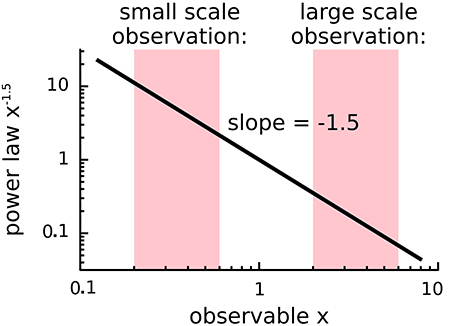
\includegraphics[width=\imsize]{fnsys-08-00166-g003.jpg}
	\caption[Representación gráfica de la independencia de escala de las leyes de potencia en una distribución de datos.]{Representación gráfica de la independencia de escala de las leyes de potencia en una distribución de datos, donde se ha utilizado la ley de potencia $f(x) = x^{-\alpha}$  con un exponente crítico de $\alpha=-1.5$ y una escala logarítmica en el eje $x$. La figura muestra que, independientemente del rango o escala utilizada para medir la distribución, se observa una ley de potencia con el mismo exponente crítico.} 	\label{fig:leypotencia}
\end{figure}


La hipótesis de criticidad en experimentos y simulaciones se basa en la presencia de leyes de potencia, que se espera se manifiesten en la mayoría de los sistemas críticos. Sin embargo, la existencia de leyes de potencia por sí sola no es suficiente para probar la criticidad \cite{goldstein_problems_2004,priesemann_can_2018}, ya que estas leyes también pueden ser explicadas por mecanismos no críticos \cite{touboul_can_2010,markovic_power_2014,noauthor_critical_2006,beggs_being_2012}. Por tanto, la identificación de leyes de potencia es un asunto delicado que requiere procedimientos de ajuste avanzados, debido a la dificultad para diferenciarlas de otras distribuciones de colas pesadas.\\

Las distribuciones de cola pesada son aquellas distribuciones de probabilidad cuyas colas son \textquote{más pesadas} que la distribución exponencial, siendo la gaussiana un subtipo de esta última. Entre los ejemplos de distribuciones de cola pesada se encuentran la distribución de Fisher-Tippett (doble exponencial), la distribución logarítmica normal y la distribución de Weibull, entre otras. Aunque se espera la presencia de leyes de potencia en sistemas críticos, estas distribuciones también pueden presentarse en otros sistemas no críticos. Por ende, para una mejor comprensión de la relevancia de las distribuciones de cola pesada en la neurociencia, se sugiere consultar la obra de Roberts et al  \cite{roberts_heavy_2015}.\\

Para abordar esta problemática, los investigadores han tenido acceso a metodologías estadísticas más sofisticadas gracias a los trabajos realizados por Clauset et al  \cite{clauset_power-law_2009} y otros estudios posteriores \cite{klaus_statistical_2011,markovic_power_2014}. Estas metodologías permiten distinguir las leyes de potencia de otras distribuciones de colas pesadas y evaluar su presencia en sistemas críticos. Sin embargo, es importante tener en cuenta que las leyes de potencia se truncan en sistemas de tamaño finito \cite{bonachela_self-organization_2010} y pueden verse afectadas por el submuestreo \cite{ribeiro_undersampled_2014}. Por lo tanto, es necesario emplear medidas cuantitativas para evaluar la diferencia entre las distribuciones de probabilidad acumulada experimental y ajustada por ejemplo  a través del parámetro $\kappa$ \cite{shew_neuronal_2009}.



\subsection{Escalamiento de  la ley de potencia de las avalanchas neuronales }

Beggs y Plenz demostraron experimentalmente que el comportamiento espontáneo de las redes corticales in vitro exhibe características consistentes con dinámicas críticas en su estudio histórico sobre avalanchas neuronales en cortes corticales interconectados con arreglos de microelectrodos (\gls{MEA}) \cite{beggs_neuronal_2003} . Una avalancha neuronal es una duración de actividad persistente que se propaga a través de la red y está marcada por períodos de silencio que preceden y siguen al período activo (ver \Cref{fig:avalancha}). En el caso de sistemas in vitro (es decir, cortes o cultivos disociados), la \textquote{actividad } puede referirse a los picos de mayor frecuencia o el \gls{LFP} de menor frecuencia, ya que se han estudiado ambas modalidades.\\

\begin{figure}[ht]
	\centering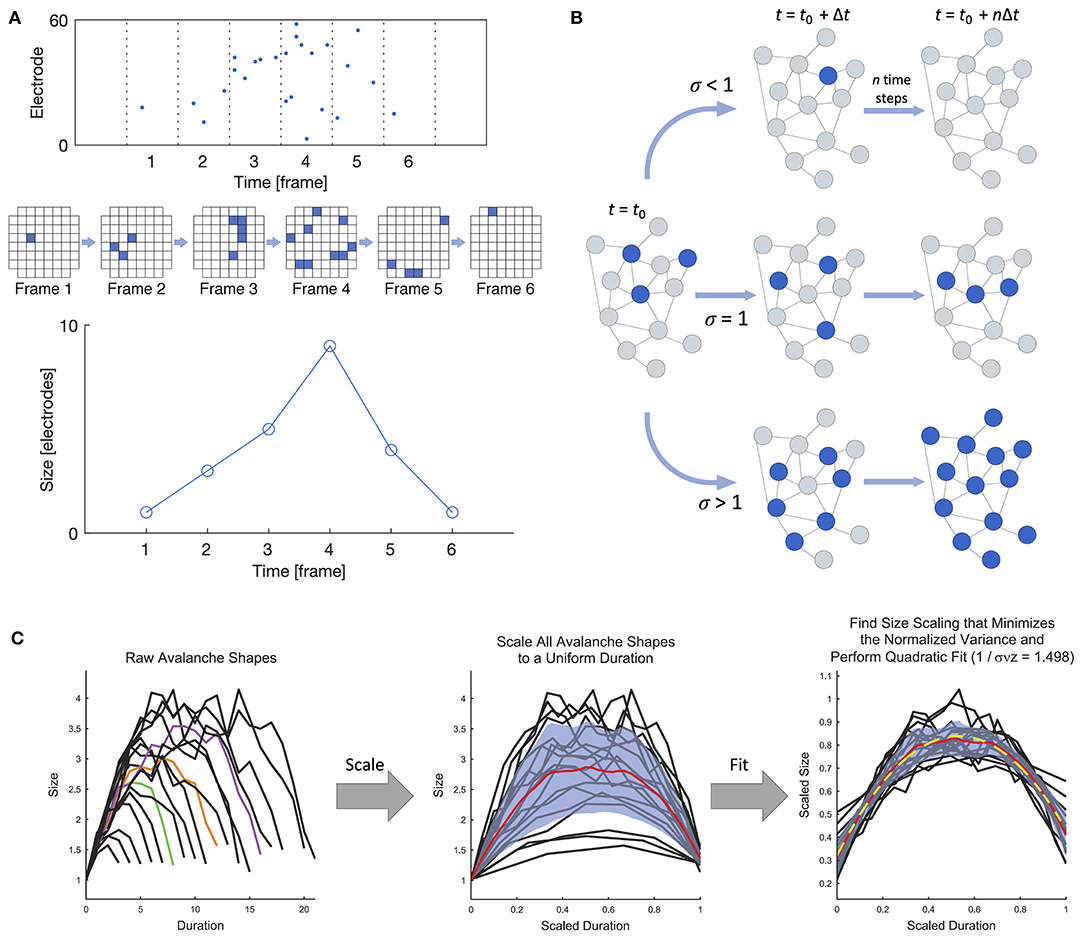
\includegraphics[width=\imsize]{fncom-15-611183-g002.jpg}
	\caption[Definición de avalancha neuronal y ejemplos de medidas empíricas de criticidad. ]{Definición de avalancha neuronal y ejemplos de medidas empíricas de criticidad. 
		(a) Se presenta la definición de avalancha neuronal, mostrando en el panel superior un gráfico rasterizado dividido en intervalos de tiempo. La avalancha representada abarca seis fotogramas activos, precedidos y seguidos por fotogramas inactivos. A continuación, se muestra una vista alternativa de la actividad en los seis marcos, en la que cada cuadrado representa un electrodo activo en una cuadrícula de 8x8. El panel inferior exhibe la definición de la forma de avalancha, la cual se obtiene a partir del número de electrodos activos en cada cuadro.
		(b) Se ilustra la relación de ramificación, en la cual los nodos azules representan actividad activa y los grises, inactiva. En una relación de ramificación de 1, la actividad persiste sin sobrecargar el sistema.
		(c) Se observa el colapso de forma en un sistema crítico, donde todas las avalanchas deberían mostrar el mismo perfil de forma temporal media en diferentes escalas de tamaño.
		Esta representación ha sido adaptada de Heiney et al.  \protect{\cite{heiney_criticality_2021}}.} 	\label{fig:avalancha}
\end{figure}


El escalamiento de la ley de potencia del tamaño $S$ y la duración $T$ de las avalanchas neuronales es un sello distintivo de la criticidad en las redes neuronales. Es decir, $P(S) \propto S^{-\alpha}$  y $P(T) \propto T^{-\beta}$, donde $P(·)$  es la función de distribución de probabilidad. El tamaño se define generalmente como el número de electrodos o neuronas activados, y la duración es el número de intervalos de tiempo activos. Los exponentes de la ley de potencia del tamaño y la duración son aproximadamente $\alpha=1.5$ y $\beta= 2.0$, respectivamente, cuando se selecciona el ancho del intervalo de tiempo para que se corresponda con el intervalo promedio entre picos. Sin embargo, la escala de la ley de potencia debe persistir en un rango de resoluciones temporales cercano al orden de magnitud del intervalo promedio entre picos, con el exponente $\alpha$ cambiando sistemáticamente con el tamaño del intervalo de tiempo seleccionado \cite{beggs_neuronal_2003,pasquale_self-organization_2008}. La escala de ley de potencia también debe mantenerse cuando se considera una resolución espacial de grano más grueso, utilizando solo un subconjunto de todos los puntos de registro. Las redes neuronales pueden mostrar varios puntos críticos dinámicos únicos, de los cuales solo uno es la transición de fase que da lugar a las avalanchas neuronales. Por lo tanto, es crucial considerar el contexto más amplio y no limitarse a la transición de fase en sí misma \cite{kanders_avalanche_2017}.







\subsection{Parámetro de ramificación}



En la teoría de los procesos de ramificación \cite{harris_theory_1963} se utiliza una medida común, la relación de ramificación $\sigma$, para evaluar el número de descendientes y ancestros en un sistema. En particular, esta medida establece la proporción entre el número de descendientes y el número de ancestros, en el que la actividad en un electrodo o neurona ancestro precede inmediatamente a la actividad en un electrodo o neurona descendiente \cite{beggs_neuronal_2003}. En un sistema en estado crítico, la relación de ramificación se aproxima a $1$, lo que permite que la actividad fluya a través de la red sin extinguirse ($\sigma < 1$) o saturar toda la red ($\sigma > 1$), tal como se muestra en la \cref{fig:avalancha}. Por tanto, la presencia de una relación de ramificación $\sigma = 1$ en respuesta a una excitación artificial en un sistema lo suficientemente inactivo puede considerarse como una evidencia de criticidad.\\

No obstante, es importante destacar que, en comparación con otras características, la evidencia proporcionada por una relación de ramificación de uno es relativamente débil. Esto se debe a que dicha relación no implica necesariamente una dinámica crítica, ya que también puede ser observada en estados supercríticos \cite{hesse_self-organized_2014}. Por lo tanto, se requiere de un análisis más riguroso que permita distinguir entre ambos estados.


\subsection{Colapso de forma}


La dinámica de los sistemas críticos se caracteriza por la presencia de avalanchas de actividad, que exhiben una naturaleza autosimilar o fractal. Se espera que la \textquote{forma} de la actividad de la avalancha se comporte como un fractal en dichos sistemas. En un estado crítico, se espera que todas las avalanchas muestren el mismo perfil temporal medio en todas las escalas. El perfil temporal de una avalancha se define como el número de sitios activos en función del tiempo. Para un sistema en estado crítico, los perfiles temporales de todas las avalanchas colapsan en la misma forma de perfil cuando se escala espacio-temporalmente con un exponente de escala$\gamma$ cercano a $2$(\Cref{fig:avalancha}). Esta propiedad se describe por  $ \left\langle S\right\rangle(T) \propto T^{-\gamma}$, donde $\left\langle S\right\rangle(T)$  representa el tamaño promedio de todas las avalanchas de una duración determinada $T$.\\

Se puede encontrar información detallada sobre el colapso de la forma en la literatura científica, como en Sethna et al \cite{sethna_crackling_2001} y Friedman et al \cite{friedman_universal_2012}. Además, Miller et al \cite{miller_scale-invariant_2019} proporciona una demostración experimental del colapso de la forma en primates no humanos. El coeficiente de criticidad (DCC) de Ma et al \cite{ma_cortical_2019} se relaciona con el concepto de colapso de forma y se calcula a partir de la diferencia entre el exponente de escala $\gamma$, obtenido a partir de datos empíricos mediante regresión lineal, y el valor esperado obtenido a partir del exponente de ley de potencia $\alpha$ de la distribución de tamaños.


\subsection{Submuestreo espacial}

Debido a la naturaleza intrínseca de la observación de los sistemas neuronales, se ve limitada la capacidad de muestrear todos los componentes del sistema. Como consecuencia, se puede obtener únicamente una muestra espacialmente submuestreada del sistema, la cual puede resultar insuficiente para obtener conclusiones precisas acerca de la dinámica subyacente del sistema. Para abordar este problema, se han desarrollado métodos que involucran el escalado del submuestreo espacial \cite{levina_subsampling_2017} y el uso de un estimador invariante de submuestreo \cite{wilting_inferring_2018}. Estos métodos permiten la evaluación precisa de los estados dinámicos de sistemas submuestreados, incluso en situaciones donde el número de componentes muestreados es significativamente menor que el número total de componentes del sistema.



\subsection{Correlación temporal de largo alcance, ralentización crítica y flickering}


En sistemas críticos, la respuesta del sistema a los estímulos externos se maximiza, lo que se conoce como rango dinámico o correlación dinámica. La criticidad del sistema genera retornos geométricos al estado estacionario \cite{hesse_self-organized_2014}, lo que resulta en una correlación temporal de largo alcance \gls{LRTC} o memoria larga. La \gls{LRTC} puede medirse de diversas maneras, siendo los métodos más populares el exponente de Hurst, a través de varios estimadores, y   \gls{DFA}  \cite{hardstone_detrended_2012}. Este último produce un exponente de escala durante un período de tiempo determinado. Un exponente de escala entre $0.5$ y $1$, con un buen ajuste, indica que la serie de tiempo exhibe \gls{LRTC} durante ese período.\\

La tasa geométrica de retorno al estado estacionario también se conoce como desaceleración crítica \cite{scheffer_early-warning_2009}. En el punto crítico, la correlación dinámica del sistema diverge de tal manera que se producen avalanchas, es decir, actividad de la red, en todas las escalas del sistema \cite{hesse_self-organized_2014}. Este fenómeno se debe a que la fluctuación en la criticidad del sistema se propaga a través de la red, generando actividad a diferentes escalas. Además, en la transición crítica, surge el fenómeno del flickering, que se produce cuando el ruido permite que un sistema migre de un lado a otro entre dos cuencas atractoras \cite{wang_flickering_2012}. En este caso, el sistema se encuentra en un estado metaestable y su comportamiento no puede ser descrito por un solo atractor.




\subsection{Ruido $(1/ f )$ y ley de potencia}

Los sistemas críticos exhiben respuestas geométricas superpuestas a entradas débiles, lo que produce ruido $1/f$, también conocido como ruido rosa, ruido de ley de potencia o ruido flicker. La dependencia de largo alcance o memoria larga se utiliza a menudo como sinónimo de estos términos, ya que se trata de fenómenos idénticos. El término ruido $1/f$ se refiere al espectro de potencia $S(f)$ de una serie temporal, el cual sigue una ley de potencia de la forma $S( f ) = \alpha f^{-\beta}$. Históricamente, se han identificado los casos $\beta=0$, $\beta=1$, $\beta=2$ como ruido \textquote{blanco}, ruido \textquote{rosa}  y ruido \textquote{marrón}, respectivamente \cite{li_fractal_2005}. El ruido $1/f$ se acepta comúnmente en el rango  $0.5 < \beta < 1.5$. Si bien todos los sistemas críticos deben exhibir ruido $1/f$, no todo el ruido $1/f$ es indicativo de criticidad \cite{bedard_does_2006,hesse_self-organized_2014}. 



\section{Discusión}

La hipótesis de la criticidad neuronal está motivada por la relación entre la criticidad y las propiedades computacionales óptimas. La hipótesis está respaldada por experimentos que observaron características de criticidad para una amplia gama de animales, en varios estados de conciencia y en muchas escalas experimentales diferentes, desde grabaciones de unas pocas neuronas hasta todo el cerebro.  Sin embargo, se ha señalado que algunas pruebas pueden ser engañosas \cite{clauset_power-law_2009} y podrían explicarse potencialmente por mecanismos alternativos \cite{botcharova_power-law_2012,galinsky_neuronal_2023}. Algunos estudios experimentales también informan resultados negativos donde no se observaron características de criticidad en la actividad neuronal  \cite{yu_scale-invariant_2014,bedard_does_2006,dehghani_avalanche_2012}. En general, la relación entre el marco teórico y su realización biológica sigue sin estar clara.  Con base con lo presentando en este capitulo , consideramos que la criticidad es preferible a las explicaciones alternativas porque proporciona una explicación motivada por la evolución para varias observaciones que de otro modo estarían desconectadas.\\

A pesar de las advertencias antes mencionadas, la creciente investigación empírica y de modelado respalda claramente la opinión de que la dinámica neuronal probablemente ocurra cerca de inestabilidades críticas. El reconocimiento de las limitaciones de este nuevo campo simplemente muestra que ha madurado más allá de las primeras etapas. El objetivo principal de este capitulo fue el de realizar una revisión de la relevancia, limitaciones y aplicaciones de la hipótesis de criticidad neuronal.   En la mayor parte de estas investigaciones tanto en los experimento  como en  el modelado  la criticidad fue analizada a nivel \textquote{macroscópico} es decir en grandes regiones del cerebro particularmente en la corteza cerebral.  Desafortunadamente no existen experimentos que analicen la criticidad neuronal a nivel de todo el sistema nervioso de un organismo. Esto en parte es debido a que las técnicas que realizan  un seguimiento de la actividad neuronal de todo el sistema nervioso  son  recientes y están limitadas a organismos simples como por ejemplo el C. elegans \cite{kato_global_2015,kaplan_nested_2020,yemini_neuropal_2021}. Otro inconveniente es que aun teniendo toda la dinámica neuronal global  de un organismo esta debe modificarse  mediante fármacos, manipulación genética u otras técnicas para verificar que el estado optimo es el cercano al estado critico, por lo que muchos animales deben utilizarse y adaptar varios protocolos experimentales a estos cambios. Por otro lado los modelos que analizan la dinámica  critica  con el  conectoma completo del C. elegans son escasos  \cite{ciftci_synaptic_2018} y ninguno de ellos  analiza la dinámica critica de todo el sistema nervioso en ausencia de estímulos y los contrasta con resultados experimentales.\\

Sabiendo las limitaciones experimentales y los pocos modelos que analizan la dinámica critica a nivel global esta parte de la tesis busca  aportar  a estas limitaciones proponiendo una solución a la pregunta ¿Existe una dinámica critica a nivel global en el C. elgans  en ausencia de estímulos
externos?. Para responder a esta pregunta  en primer lugar  se aplicaran  algunas de las métricas experimentales de criticidad presentadas en este capitulo  en  datos experimentales de la dinámica neuronal global de  gusanos inmovilizados suministrados por (Kato et al) \cite{kato_global_2015}, (Kaplan et al)  \cite{kaplan_nested_2020} y neuropal \cite{yemini_neuropal_2021}.  El  objetivo especifico es analizar en que región se encuentra los datos experimentales de las   dinámicas neuronales del C. elgans.  Nuestra hipótesis de trabajo es que aun en un organismo tan pequeño como lo es el C. elegans la dinámica neuronal se encuentran en un régimen dinámico cercano al punto crítico de una transición de fase de segundo orden.\\


Por otro lado para superar las limitaciones experimentales de no poder manipular en tiempo real la dinámica neuronal y  tener un mayor control de los parámetros del sistema se plantea un modelo utilizando  el Conectoma  realizado por Cook y coautores  \cite{cook_whole-animal_2019} el cual abarca  todas las conexiones  neuronales  del C. elegans  junto a una  dinámica neuronal descrita por una regla dinámica no lineal muy simple la cual es una  adaptación del modelo neural Greenberg-Hastings introducida por Haimovici y coautores  \cite{haimovici_brain_2013}.   El  objetivo específico busca cuantificar la dinámica critica  en términos de un parámetro de orden   que emerge al manipular tanto los parámetros de  la dinámica neuronal  como el parámetro de control del sistema.  La hipótesis de trabajo es que los patrones espacio temporales observados de manera experimental en la actividad cerebral en ausencia de estímulos  solo pueden ser descriptos por un modelo de red neural si la misma se encuentra en un estado crítico. Finalmente, como objetivo específico buscaremos establecer relaciones entre los resultados experimentales y  nuestro modelo. En el siguiente capitulo se introducirá  mediante la teoría de percolaciones  el parámetro de orden que  nos permitirá caracterizar la transición de fase que surge al aplicar una dinámica critica al conectoma del C. elegans. 









%%% Local Variables: 
%%% mode: latex
%%% TeX-master: "template"
%%% End: 

\chapter{Teoría de la percolación y parámetro de orden}\label{titulo-cap-percolacion}
\graphicspath{{figs/capitulo_percolacion/}}

\chapterquote{For power laws hint that a system may be organizing itself. They arise at phase transitions, when a system is poised at the brink, teetering between order and chaos. They arise in fractals, when an arbitrarily small piece of a complex shape is a microcosm of the whole }{Steven H. Strogatz}


\section{Introducción}

En el capítulo anterior se expusieron los fundamentos de la hipótesis de la criticidad neuronal, respaldada por evidencias experimentales, y se presentaron las medidas utilizadas para caracterizar el estado crítico de un sistema. En los capítulos siguientes, se aplicarán estas medidas al estudio de la dinámica neuronal en experimentos con  C. elegans, así como en un modelo que simula una dinámica neuronal crítica basada en su conectoma. El objetivo principal de estos análisis es comprobar o refutar la hipótesis de que el cerebro de este organismo se encuentra en un estado crítico en la frontera entre distintos tipos de dinámicas.

Con el fin de alcanzar dicho objetivo, se procederá a la construcción de un diagrama de fase mediante la variación de los parámetros del modelo.  Como se discutió previamente, el diagrama de fase constituye una evidencia directa de las transiciones de fase en el sistema. Para lograr una caracterización precisa de este diagrama, resulta fundamental contar con un parámetro de orden que permita cuantificar el grado de organización del sistema. Estos parámetros de orden son variables que describen la ruptura de simetría entre fases ordenadas (más simétricas) y desordenadas  (menos simétricas), y deben cumplir dos requisitos esenciales: en primer lugar, presentar valores distintos para las diferentes fases; y en segundo lugar, mostrar un salto en su momento de segundo orden (susceptibilidad) en los puntos de transición  \cite{yin_neural_2021}. La elección adecuada de un parámetro de orden, que pueda medirse experimentalmente y esté estrechamente relacionado con el \textquote{grado de orden}, se convierte así en un aspecto crucial y delicado en este análisis \cite{kleman_order_2003}.




Según lo  mencionado en la parte I, Kato et al \cite{kato_global_2015}  han demostrado la  participación significativa de las neuronas en el cerebro de C. elegans en una actividad de red dinámica y coordinada cuando los animales se encuentran inmovilizados. De esta manera, resulta sumamente interesante caracterizar el diagrama de fase del modelo utilizando un parámetro de orden que permita cuantificar los clústeres de neuronas sincronizadas en la dinámica neuronal. Afortunadamente, en el ámbito de la física estadística, existe una teoría  conocida como teoría de la percolación que aborda precisamente este problema. La teoría de la percolación se enfoca en los efectos derivados de la variación de la conectividad de los elementos en un sistema aleatorio y describe la aparición de conectividad de largo alcance al alcanzar un umbral de percolación \cite{torquato_percolation_2002}. Esta teoría, respaldada por leyes de escala, fractales, criticidad y renormalización, posee una gran relevancia teórica en diversos campos de la física. A lo largo del tiempo, la percolación ha sido ampliamente utilizada como un modelo básico para demostrar transiciones de fase y fenómenos críticos \cite{li_percolation_2021}. En el contexto de la percolación, se plantean tres interrogantes fundamentales:

\begin{enumerate}[label={(\alph*)}]
\item  ¿Cuál es la propiedad geométrica o física relevante que influye en la conectividad del sistema en estudio? Por ejemplo, uno puede considerar la sincronización neuronal como un factor determinante.
\item ¿Cuál es el umbral de percolación ($p_c$) específico para dicho sistema?
\item  ¿Cuál es el exponente que describe el comportamiento del parámetro de orden en las proximidades del umbral de percolación ($p_c$)?
\end{enumerate}

Un aspecto particularmente fascinante y útil de la teoría de la percolación radica en la presencia de un exponente crítico compartido por muchos sistemas. Esto implica que al encontrar y resolver un modelo simple, se puede predecir el valor de este exponente para sistemas más complejos. A esta propiedad, conocida como \textquote{universalidad}, se le atribuye una importancia central en la teoría de la percolación. No obstante, es importante señalar que el umbral de percolación debe determinarse de forma específica para cada sistema, aunque existen pautas generales que pueden resultar útiles en dicho proceso \cite{berkowitz_percolation_1998}.

En este capítulo, se busca proporcionar una caracterización precisa de la sincronización neuronal mediante el uso de un parámetro de orden. Para lograr este objetivo, se recurre a la teoría de la percolación como una introducción a los enfoques basados en clústeres para el análisis de fenómenos colectivos. En la física estadística, los sistemas que involucran interacciones entre unidades, como moléculas o espines, presentan dificultades para ser resueltos de manera exacta, mientras que aquellos sin interacciones son más fáciles de abordar. Por lo tanto, se utiliza frecuentemente la aproximación de clústeres, que permite transformar el problema de unidades interactuantes en uno de clústeres no interactivos \cite{stauffer_scaling_1979}.

Para respaldar de manera sólida los modelos de clústeres en transiciones de fase generales, se estudian modelos simplificados en lugar de utilizar unidades reales. Esta estrategia brinda la posibilidad de examinar directamente los clústeres microscópicos y su influencia en magnitudes macroscópicas, como la susceptibilidad, entre otras. Sin embargo, para que un modelo de clústeres sea efectivo, debe cumplir con cinco propiedades fundamentales:

 \begin{enumerate}[label=(\roman*)]
	\item  Cada configuración debe presentar una separación clara y natural de las unidades en clústeres.
	\item  La definición de clústeres debe ser lo suficientemente simple como para permitir su implementación computacional.
	\item  Se deben poder calcular de manera confiable algunas magnitudes macroscópicas a partir de las propiedades de los clústeres.
	\item  El sistema debe tener un punto crítico en el que se formen clústeres grandes.
\end{enumerate}


En linea con lo anterior, se propone un modelo que involucra la interacción de unidades neuronales agrupadas en clústeres dentro de un marco estructural conocido como conectoma. Estas interacciones generan cambios en el estado de las neuronas, activándolas o desactivándolas, lo que a su vez provoca modificaciones en la topología de la red. El objetivo principal de este capítulo es caracterizar los clústeres neuronales a través del uso de observables geométricos y describir las propiedades correspondientes a diferentes fases: subcrítica, crítica y supercrítica.


En el \cref{sec:fenomenologia}, se presentan de forma concisa las definiciones básicas, los conceptos fundamentales y los resultados clave de la percolación discreta. A continuación, en el \cref{sec:matematicaspercolacion}, se realiza un análisis exhaustivo de los aspectos matemáticos relevantes de la teoría de la percolación, estableciendo la probabilidad de percolación $P_\infty(p)$. El \cref{sec:percolacion_critico} se enfoca en la teoría de la percolación como fenómeno crítico, donde se definen propiedades fundamentales como la distribución del tamaño de los clústeres $n_s(p)$ y la susceptibilidad $\chi(p)$, que está relacionada con el tamaño promedio de los clústeres. Además, se introduce un parámetro de orden para caracterizar de manera precisa el diagrama de fase del modelo propuesto. En esta sección también se exploran los fundamentos teóricos de propiedades importantes cerca del umbral de percolación, como las leyes de escala, los fractales y el comportamiento a escala finita.

Para una comprensión más profunda de los aspectos teóricos y matemáticos de la teoría de la percolación, se recomienda consultar las referencias proporcionadas \cite{dorogovtsev_critical_2008,rong_estimation_2022,newman_networks_2018,ariel_percolation,Hugo_percolation,hammersley_percolation_1980,bunde_fractals_2012,grimmett_probability_2018,albert_statistical_2002,boccaletti_structure_2014}.


\section{Fenomenología}\label{sec:fenomenologia}


La teoría de la percolación se centra en el análisis de la conectividad global en sistemas compuestos por múltiples objetos, los cuales se conectan a través de reglas locales restringidas por una topología subyacente. Su objetivo fundamental es comprender cómo emerge el comportamiento global a partir de las interacciones locales en dichos sistemas \cite{hunt_percolation_2014}. En la literatura, se encuentran los trabajos pioneros sobre percolación, destacándose los estudios clásicos realizados por Flory y Stockmayer, quienes investigaron fenómenos como la polimerización y la transición sol-gel \cite{flory_molecular_1941,stockmayer_theory_2004}. A medida que la teoría de la percolación se desarrolló, se establecieron conexiones con las teorías de grafos y redes, situándose en la intersección de la teoría de la probabilidad y la topología.

En el contexto de nuestro modelo de criticidad neuronal, la teoría de la percolación adquiere una relevancia fundamental, ya que nos permite obtener información sobre propiedades globales a partir de especificaciones locales. Sin embargo, comprender las relaciones entre las propiedades locales y globales no es una tarea trivial debido a la complejidad inherente de los sistemas estudiados. Estas propiedades globales pueden estar relacionadas tanto con características topológicas universales como con particularidades específicas del sistema analizado.

Dentro de la teoría de la percolación, la topología se refiere a la estructura espacial $d$-dimensional que existe de manera independiente a las características probabilísticas. Un ejemplo común de estas estructuras son las redes regulares, donde los nodos o sitios se interconectan mediante enlaces. Sin embargo, en la teoría de la percolación se introduce un componente probabilístico en la existencia de estos enlaces (nodos), generando topologías más complejas derivadas de las estructuras conocidas. Se presentan tres variantes fundamentales de la teoría de la percolación: percolación de enlace, percolación de sitio y percolación continua, estando estrechamente relacionadas con las redes previamente mencionadas. Además, existen variantes interesantes y potencialmente relevantes, como la percolación de bootstrap \cite{chalupa_bootstrap_1979}, la percolación de gradiente \cite{rosso_gradient_1986} y la percolación de invasión \cite{chandler_capillary_1982,nickel_invasion_1983,wilkinson_invasion_1983}.


\subsection{Percolación de enlaces y sitios}



La percolación se refiere al fenómeno de formación de un componente conexo de gran tamaño en un grafo. Inicialmente, este proceso fue estudiado en grafos infinitos, donde los vértices representan el conjunto $\mathbf{Z}^d$  y los bordes conectan cada vértice con sus vecinos más cercanos. Sin embargo, también se consideran grafos aleatorios más generales en investigaciones recientes.

En este contexto, se introduce el parámetro $p$, que indica la probabilidad de que una arista en el grafo esté abierta o cerrada. Cada arista se considera independiente de las demás, con una probabilidad de cierre de $1-p$. Desde un punto de vista práctico, se distingue entre la percolación de enlaces, que se refiere al estado abierto o cerrado de las aristas, y la percolación de sitios, que se enfoca en la apertura o cierre de los vértices.

A medida que se varía el valor de p en el proceso de percolación de $0$ a $1$, se llega a un punto en el que surge un componente abierto gigante, conocido como clúster gigante o clúster expansivo. Este fenómeno ocurre cuando se alcanza el umbral de percolación, $p_c$. La probabilidad de percolación muestra un comportamiento escalonado alrededor de $p_c$, siendo igual a $1$ para $p > p_c$ y 0 para $p \leq p_c$. Aunque en $p = p_c$ no existe un clúster infinito, es común observar la presencia de clústeres muy grandes cerca de este punto (ver \Cref{fig:probabilidadinf}) \cite{aizenman_number_1997}.


 \begin{figure}[ht]
	\centering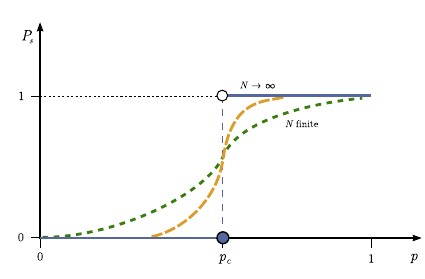
\includegraphics[width=\imsize]{probabilidad}
	\caption[Gráfico esquemático que ilustra la relación entre la probabilidad de percolación y la ocupación en un sistema]{Gráfico esquemático que ilustra la relación entre la probabilidad de percolación y la ocupación en un sistema. A medida que el tamaño del sistema ($N$) se aproxima a infinito, la probabilidad de percolación ($P_\infty$) converge hacia una función escalonada alrededor del umbral crítico ($p_c$). En determinados casos de sistemas altamente específicos, se observa una intersección en un punto único para todos los gráficos correspondientes a valores finitos de $N$. Sin embargo, debido a las correcciones de tamaño finito inherentes, en general esta intersección no ocurre en un único punto para sistemas finitos.}\label{fig:probabilidadinf}
\end{figure}

Es relevante destacar que, en general, los enlaces de una red tienen más vecinos cercanos que los sitios. Por lo tanto, los clústeres de enlaces se forman de manera más eficiente que los clústeres de sitios, lo que implica que se requiere una menor concentración de enlaces para generar un clúster expansivo. En otras palabras, el umbral de percolación de los enlaces es menor que el umbral de percolación de los sitios en una red dada \cite{bunde_fractals_2012}.



Dentro del campo de la percolación, un tema de investigación activo es la determinación precisa de los umbrales de percolación, ya sea mediante métodos exactos o simulaciones. Estos umbrales son una característica fundamental en la teoría de la percolación y su valor no es universal, sino que depende en gran medida de la estructura del grafo subyacente y su dimensionalidad. Se postula que los umbrales alcanzan valores de campo medio solo en el límite de dimensionalidad infinita \cite{Artem,fisher_clúster_2004}. Encontrar pruebas rigurosas de los umbrales y límites exactos ha sido un desafío constante para los investigadores \cite{kesten_critical_1980,wierman_bond_1984,grimmett_percolation_2013}. Aunque se han obtenido los umbrales exactos en 2D para redes cuadradas, triangulares, de panal y estructuras similares utilizando la transformación estrella-triángulo (ver \Cref{table:umbral}) \cite{wierman_bond_1984}, aún existen numerosos sistemas de interés para los cuales los umbrales exactos son desconocidos

 
 \begin{table}[h!]
 	\centering
 	\caption[Umbrales de percolación para varias redes en diferentes dimensiones y la red de Bethe. ]{ Umbrales de percolación para varias redes en diferentes dimensiones y la red de Bethe. La segunda columna enumera el número de vecinos más cercanos (nn), también conocido como número de coordinación. En una dimensión dada, se observa una disminución del umbral de percolación a medida que aumenta el número de vecinos más cercanos. La red o árbol de Bethe es una red no periódica infinita sin bucles cerrados (circuitos), en la cual cada sitio (excepto los múltiples sitios en la superficie) tiene un número de coordinación $Z$, que representa el número de enlaces conectados a dicho sitio.
 	}
 	\begin{tblr}{colspec={X[l,2]X[l,1]X[l,3]X[l,3]},
 			row{odd} = {bg=gray8},
 			row{even} = {bg=gray9},
 			row{1} = {bg=red3, fg=white, font=\sffamily},
 		}
 		
 		red	&  \# nn  &  {Percolación \\ de sitios}  &   {Percolación \\ de enlaces} \\
 		1d & $2$  & $1$ & $1$ \\
 		Triangular (2d) & $6$ &  $1/2$ & $2\sin(\pi/18)\approx 0.34729$ \\
 		Cuadrada (2d) &  $4$ &  $0.592746$ &  $1/2$ \\
 		Panal (2d)        &  $3$ &  $0.6962$ &  $1-2\sin(\pi/18)\approx0.65271$ \\
 		FCC (3d)           &  $12$ &  $0.198$   &  $0.119$ \\
 		BCC (3d)          &  $8$ & $0.246$    &  $0.1803$ \\ 
 		CS (3d) & $6$ &  $0.31161$ &  $0.248814$ \\
 		Diamante (3d) & $4$ & $0.43$ & $0.388$ \\
 		Hipercubo (4d) & $8$ & $0.197$ & $0.1601$ \\
 		Hipercubo (5d) & $10$ & $0.141$ & $0.1182$ \\
 		Hipercubo (6d) & $12$ & $0.107$ & $0.0942$ \\
 		Hipercubo (7d) &  $14$ & $0.089$ &  $0.0787$ \\
 		red de Bethe &  $z$ & $1/(z-1)$  &  $1/(z-1)$  \\
 	\end{tblr}
 	\label{table:umbral}
 \end{table}
 
 
 
 Consideremos un fragmento de la red cuadrada  $\mathbf{Z}^2$ como ejemplo ilustrativo de la definición anterior. En esta red, los puntos de intersección de las líneas se denominan \textquote{sitios}, mientras que los segmentos que los conectan se conocen como \textquote{enlaces}. En una red cuadrada, cada enlace se encuentra conectado a los seis enlaces vecinos más cercanos, mientras que cada sitio solo tiene cuatro sitios vecinos más cercanos. Se asume que cada sitio puede estar en uno de dos estados posibles: \textquote{vacío} o \textquote{abierto} (también se podría utilizar la terminología de \textquote{permitido}, aunque no existe una terminología universalmente aceptada para estos estados, y se podrían emplear términos como \textquote{encendido} o \textquote{apagado}). Además, se considera que la apertura de un sitio ocurre de manera aleatoria e independiente de sus vecinos, con una probabilidad $p$. En esta red, cada par de sitios vecinos más cercanos está conectado por un enlace. Cuando se observa que un poco más de la mitad de los sitios están abiertos (\Cref{fig:percolacion_enlaces_sitios}b, centro), se evidencia una tendencia de los sitios abiertos a agruparse en clústeres de diversas formas y tamaños. Estos clústeres pueden ser clasificados de acuerdo a su tamaño. Por ejemplo, un grupo de tamaño $1$ corresponde a un solo sitio abierto sin vecinos abiertos inmediatos, mientras que un grupo de tamaño $2$ consiste en dos sitios abiertos adyacentes sin vecinos abiertos, y así sucesivamente.
 
 
 
 Cuando la probabilidad $p$ se incrementa a $0.605$ (\Cref{fig:percolacion_enlaces_sitios}b, derecha), se observan varios fenómenos significativos. 
 En primer lugar, con una probabilidad entre $1/2$ y $2/3$, muchos de los sitios se unen en un \textquote{clúster gigante} que abarca tanto la matriz en sentido vertical como horizontal . Esta probabilidad crítica $p_c$, es aproximadamente $p_c \approx 0.593$  para los sitios de la red cuadrada. Un enfoque analógico se puede realizar considerando un \textquote{fluido} que únicamente puede fluir a través de los enlaces que conectan sitios abiertos. Por debajo del umbral de la probabilidad crítica, la red presenta una conductividad cero, mientras que por encima de dicho umbral, la conductividad aumenta a medida que se incrementa la probabilidad. De esta manera, se establece una fuerte relación entre la conectividad de los elementos microscópicos del sistema y las propiedades físicas a nivel macroscópico. Además, a medida que se incrementa la proporción de sitios abiertos, también aumenta la proporción de sitios vacíos con vecinos abiertos. Este aumento en la proporción de sitios vacíos conectados a vecinos abiertos tiene implicaciones significativas en el comportamiento global del sistema.
 
  

\begin{figure}[ht]
	\centering\includegraphics[width=\imsize]{percolacion_enlaces_sitios.png}
	\caption[Diagramas esquemáticos que ilustran la percolación clásica en una red cuadrada.]{Diagramas esquemáticos que ilustran la percolación clásica en una red cuadrada. En estos diagramas, se utilizan diferentes colores para representar clústeres distintos. El tamaño del sistema utilizado es $N = L \times L = 80 \times 80$. Los valores de $p$ etiquetados en las figuras corresponden a las probabilidades de ocupación de los sitios o enlaces correspondientes. (a), se muestra la percolación de enlaces, donde se omiten los sitios y enlaces no ocupados para facilitar la identificación. Para un valor de $p = 0.51$, se observa la existencia de un clúster gigante destacado en color amarillo.(b), se ilustra la percolación de sitios, nuevamente omitiendo los enlaces y sitios no ocupados para una mejor visualización. Para $p = 0.605$, se identifica un clúster gigante en color azul (adaptado de \protect\cite{li_percolation_2021}).}\label{fig:percolacion_enlaces_sitios}
\end{figure}


Una vez que se supera el umbral crítico $p_c$, se observa que el flujo de fluido en la red ocurre exclusivamente a través de los enlaces que conectan los sitios abiertos. Al examinar la estructura resultante, se evidencia la presencia de una columna vertebral compuesta por enlaces que permiten el flujo continuo del fluido, mientras que otros enlaces se convierten en callejones sin salida aislados o ramas colgantes. La proporción de estas ramas varía en función del valor de $p$. La función de accesibilidad se define como la proporción de sitios abiertos que forman parte del clúster infinito, es decir, aquellos que serían atravesados por el fluido en los límites de la red.  A medida que incrementa el valor de $p$, los clústeres experimentan un crecimiento y se fusionan entre sí, mientras que los sitios vacíos se fragmentan y se agrupan en clústeres más pequeños. Cabe destacar que el ejemplo mencionado anteriormente corresponde a la percolación de sitios, donde se varía exclusivamente la proporción de sitios abiertos. Existe también un procedimiento similar conocido como percolación de enlaces, en el cual se varía la proporción de enlaces abiertos (\Cref{fig:percolacion_enlaces_sitios}a). Es importante tener en cuenta que estos dos procedimientos no son intercambiables y no existe una fórmula simple que permita predecir la percolación de enlaces a partir de la percolación de sitios. Además, el valor crítico $p_c$ para la percolación de sitios siempre es mayor que el valor crítico $p_c$ para la percolación de enlaces (consultar \Cref{table:umbral}).


El contorno irregular y \textquote{ramificado} de un clúster en percolación presenta similitudes con los fractales. De hecho, se ha demostrado que los clústeres cercanos al umbral de percolación exhiben propiedades fractales \cite{aharony_introduction_2017}. La dimensión fractal de un clúster de percolación es aproximadamente constante ($D \approx 1.896$) independientemente del tipo de red bidimensional utilizada, ya sea cuadrada, triangular, de panal, de Voronoi u otra (\Cref{fig:distitnasredes}a–d), a pesar de las diferencias en sus conectividades, las cuales pueden ser cuantificadas mediante el número de coordinación $z$, definido como el promedio de enlaces por sitio. No obstante, la dimensión fractal varía según la dimensionalidad o la dimensión de incrustación $d$ de la red. Por ejemplo, los clústeres que se percolan en redes bidimensionales presentan dimensiones fractales distintas a las de las redes tridimensionales, como las redes cúbicas (\Cref{fig:distitnasredes}e).



\begin{figure}[ht]
	\centering\includegraphics[width=\imsize]{distitnasredes.png}
	\caption[Ejemplos de redes bidimensionales.]{ Ejemplos de redes bidimensionales, en las cuales los sitios son representados por círculos, mientras que los enlaces se muestran mediante líneas oscuras. En esta figura, se exhiben diversas configuraciones de redes: (a) una red cuadrada con  $z=4$, (b) una red triangular con  $z=6$, (c) una red tipo panal con $z=3$, (d) una red Voronoi con un grado promedio de conectividad de $\left\langle z \right\rangle = 6$, (e) una red cúbica con  $z=6$, y (f) un árbol de Cayley con  $z=3$ (adaptado de \protect\cite{berkowitz_percolation_1998})}\label{fig:distitnasredes}
\end{figure}






\section{Fundamentos matemáticos de la percolación}\label{sec:matematicaspercolacion}

Se considera un grafo $\mathcal{G}=(\mathcal{V},\mathcal{E})$, donde $\mathcal{V}$ representa el conjunto de vértices y $\mathcal{E}$ el conjunto de aristas. En el marco del modelo de percolación de enlace, cada arista tiene la capacidad de abrirse de manera independiente con una probabilidad $p$ o cerrarse con una probabilidad $1-p$. Este fenómeno se describe mediante la medida de probabilidad $P_p$. El conjunto de aristas abiertas forma así un subgrafo aleatorio de $\mathcal{G}$ y la pregunta original formulada por Broadbent se centra en determinar si la componente conexa del origen en este subgrafo aleatorio es finita o infinita \cite{beffara_percolation_2006}.



Se define un camino en $\mathcal{G}$ como una secuencia $v_1, v_2, \cdots$ en la cual cada par de vértices sucesivos, $v_i$ y $v_{i +1}$, se encuentran conectados mediante una arista en $\mathcal{G}$. Un camino se considera abierto si todas las aristas $\left\{v_i,v_{i+1}\right\}$ que lo componen están en estado abierto. El clúster infinito del origen se refiere a la existencia de un camino abierto ilimitado que se origina en el vértice de origen. Además, se presenta un modelo análogo denominado percolación del sitio, en el cual todas las aristas son transitables, aunque cada vértice puede encontrarse en estado abierto o cerrado de manera independiente, con probabilidades $p$ y $1 - p$, respectivamente. En este caso, se define un camino abierto como aquel en el cual todos los vértices a lo largo del camino se encuentran en estado abierto.

 Se asume que todos los grafos considerados son conexos, localmente finitos y cuasi-transitivos. Si $A$ y $B$ son subconjuntos de vértices en $\mathcal{V}$, se establece que $A\leftrightarrow B$ si existe un camino abierto que conecta algún vértice en $A$ con algún vértice en $B$. Para simplificar la notación, se utiliza la notación $u \leftrightarrow v$ para denotar la existencia de un camino entre los vértices $u$ y $v$, es decir, el evento $\left\{u\right\} \leftrightarrow \left\{v\right\}$. El clúster abierto $C(v)$  de un vértice $v$ se define como el conjunto de todos los vértices abiertos que se encuentran conectados a $v$ mediante un camino abierto:

\begin{equation}\label{eq:1}
	C(v) = \left\{u\in \mathcal{V}: u \leftrightarrow v \right\}
\end{equation}

La probabilidad de percolación $\theta(p)$  se considera el parámetro central en la teoría de la percolación, y representa la probabilidad de que un sitio seleccionado aleatoriamente pertenezca a un clúster infinito \cite{torquato_percolation_2002}. Es importante resaltar que $\theta(p)$  siempre es menor que $p$, excepto en el caso trivial cuando $\theta(p) = p = 1$. En un sistema infinito, la probabilidad de percolación es cero para valores de $p$ por debajo de $p_c$.


\begin{equation}\label{eq:2}
\theta(p)  \equiv P_\infty = P_p\left\{\mathbf{0} \leftrightarrow \infty\right\} = P_p\left\{\left| C(\mathbf{0})\right|=\infty \right\}  = \begin{cases}
	0 & \text{sí } p<p_c\\
	>0 & \text{sí } p>p_c
\end{cases}
\end{equation}

El modelo de percolación se distingue por su propiedad más destacada: la presencia de una transición de fase geométrica, en la cual el parámetro $\theta(p)$ desempeña el papel de un parámetro de orden en una transición de fase termodinámica. Esta transición se produce en un valor crítico $p_c \in  [0 , 1]$, donde el comportamiento global del sistema experimenta cambios sustanciales en dos regiones distintas: $p < p_c$ y $p > p_c$.  Para definir esta propiedad de forma rigurosa, se emplea la construcción conjunta de sistemas de percolación de Hammersley \cite{broadbent_percolation_1957}  en el grafo $\mathcal{G}$. Se considera una colección de variables aleatorias independientes $\left\{U(v),v\in\mathcal{V}\right\}$, distribuidas uniformemente en el intervalo $[0,1]$. Un vértice $v$ se declara como $p$-abierto si $U(v) \leq p$; de lo contrario, se declara como $p$-cerrado. La configuración de vértices $p$-abiertos sigue la distribución $P_p$ para cada valor de $p\in [0, 1]$. Es relevante destacar que la colección de vértices $p$-abiertos no disminuye a medida que $p$ aumenta, lo que implica que $\theta(p)$ también es una función no decreciente. Esta propiedad se puede demostrar observando que $\theta(0) = 0$ y $\theta(1) = 1$  (ver \Cref{fig:probabilidadtheta}). Por lo tanto, $\theta(p)$  juega un papel fundamental como parámetro de orden en la transición de fase.



\begin{figure}[ht]
	\centering\includegraphics[width=\imsize]{probabilidadtheta.png}
	\caption[El comportamiento de la función $\theta(p)$ en las cercanías del punto crítico.]{El comportamiento de la función $\theta(p)$ en las cercanías del punto crítico.}\label{fig:probabilidadtheta}
\end{figure}


El valor crítico o umbral de percolación $p_c$ se define formalmente (para un sistema infinito) como:

\begin{equation}\label{eq:3}
p_c \equiv p_c( \mathcal{G}) = \sup\left\{p:\theta(p)=0\right\},
\end{equation}


donde $\sup$ representa el supremo, es decir, el límite superior mínimo. Cuando $p < p_c$, el clúster abierto que contiene el origen es finito, lo que implica que todos los clústeres también son finitos. En contraste, cuando $p > p_c$, la distribución $P_p$ presenta una probabilidad estrictamente positiva de que el clúster que contiene el origen sea infinito. Por lo tanto, $p_c$ marca la transición en la cual el comportamiento global del sistema experimenta un cambio significativo.



\begin{theorem}[Ley Cero-Uno de Kolmogórov] % Specify a name/title in square brackets, or leave them out for no title
	Sea $\omega(e)_e$  una secuencia de variables aleatorias independientes e idénticamente distribuidas, y $A$ un evento de cola. Entonces, se cumple que $\mathbb{P}[A] \in {0, 1}$ .
\end{theorem}

La Ley Cero-Uno de Kolmogórov establece que 

\begin{equation}\label{eq:4}
P_p\left\{\left| C(v)\right| =\infty \ \text{para algún} \ v \in  \mathcal{V}  \right\} = 1 \ \text{para} \quad p>p_c
\end{equation}

Esta ley implica que cuando el valor de $p$ supera el umbral $p_c$, se garantiza que al menos un vértice $v \in \mathcal{V}$ pertenezca a un clúster de tamaño infinito.
Por lo tanto, si los intervalos $[0, p_c)$ y $(p_c, 1]$ no están vacíos, se produce una transición de fase en $p_c$. Esta transición de fase indica un cambio cualitativo en el comportamiento del sistema al cruzar el umbral $p_c$.  Utilizando el argumento de Peierls, es posible demostrar de manera sencilla que $p_c(\mathcal{G} )$ es mayor que cero para cualquier grafo $\mathcal{G}$ con un grado acotado. Este resultado implica que en todos los grafos $\mathcal{G}$  con grados acotados, se establece un valor umbral $p_c$ por encima del cual el sistema exhibe una fase supercrítica, donde es probable la existencia de clústeres de tamaño infinito.


\section{La percolación como fenómeno crítico}\label{sec:percolacion_critico}


En la sección anterior, se exploró la percolación como una transición de fase geométrica  que ocurre cuando la concentración crítica $p_c$ divide el sistema en dos fases distintas: una con clústeres finitos ($p < p_c$) y otra con un clúster de gran tamaño ($p > p_c$). Es importante destacar que una verdadera transición de fase se presenta únicamente en sistemas infinitos, conocidos como el \textquote{límite termodinámico}. En este contexto, la concentración crítica $p_c$ se define de forma única en sistemas infinitos. La transición de percolación se caracteriza por las propiedades geométricas de los clústeres cercanos a $p_c$. Un parámetro clave en este sentido es la probabilidad $P_\infty$, definida mediante la  \cref{eq:2}. Esta probabilidad es nula por debajo de $p_c$ y distinta de cero por encima de $p_c$. Para valores ligeramente superiores a $p_c$, se establece una relación de la forma

 \begin{equation}\label{eq:10}
	P_\infty \propto \left(p-p_c\right)^\beta,
\end{equation}

donde $\beta$ es el \textquote{exponente crítico}. El comportamiento crítico en la teoría de la percolación se refiere al estudio de la red infinita y los clústeres grandes pero finitos en las cercanías de $p_c$, también conocido como región de escalamiento. En esta región, se observa un comportamiento crítico independiente de las propiedades locales del sistema, como el tipo de red y el mecanismo de percolación. Esto se debe al principio de universalidad, que establece que el valor de $p_c$ está determinado por la estructura local del sistema, mientras que el comportamiento de los clústeres cercanos a $p_c$ es independiente de dicha estructura local. En consecuencia, la percolación se considera un fenómeno dependiente del sustrato pero independiente del modelo específico. Los exponentes críticos, como $\beta$, son determinados exclusivamente por la geometría del sistema y son idénticos tanto en la percolación de enlaces como en la percolación de sitios.

 \subsection{Parámetro de orden}\label{sec:parametro_orden}
 
 
 
 
 
La teoría de escalamiento de los clústeres de percolación es el enfoque más elegante para caracterizar la percolación como un fenómeno crítico \cite{stauffer_scaling_1979}. En términos de estadísticas de clústeres, se puede formular gran parte de la teoría de la percolación, lo que facilita establecer analogías con otras transiciones de fase. En este sentido, se propone la definición de un parámetro de orden que permita caracterizar nuestro modelo de criticidad neuronal a través de observables geométricos. En el contexto de la percolación, los clústeres desempeñan un papel fundamental.
 
 
\begin{definition}[clúster] % Specify a name/title in square brackets, or leave them out for no title
Un clúster se define como  un conjunto de componentes o elementos interconectados en una red, donde la conexión entre ellos se establece mediante vínculos o relaciones específicas.
\end{definition}

Se consideran clústeres de tamaño unitario a los nodos aislados, mientras que se denomina $s$-clúster a cualquier conjunto de $s$ nodos conectados. El análisis de la percolación se centra en la aparición del clúster infinito a medida que aumenta la probabilidad $p$. Una medida común para caracterizar este fenómeno es la probabilidad $\bar{S}_1/N$ de que un nodo pertenezca al clúster infinito, donde $N$ representa el tamaño del sistema (número de sitios) y $\bar{S}_1$ es el promedio en ensamble del número de sitios $S_1$ en el clúster más grande.  Como se ilustra en la \cref{fig:probabilidadtheta}, a medida que $p$ aumenta, también lo hace la probabilidad de encontrar clústeres de mayor tamaño. En una red finita, como se muestra en la \cref{fig:percolacion_enlaces_sitios}, se identifica un valor crítico $p_c$ por encima del cual al menos un clúster conecta los extremos \textquote{inferior} y \textquote{superior} (o \textquote{izquierdo} y \textquote{derecho}) de la red. En otras palabras, se establece un punto crítico $p_c$ para el cual $\bar{S}_1/N$ adquiere un valor distinto de cero. En el campo de la ciencia de redes, el tamaño del clúster más grande se considera un parámetro de orden preferido. En el umbral de percolación, este parámetro de orden muestra un comportamiento crítico a medida que el sistema tiende al límite $N \to\infty$. Dicha relación puede expresarse de la siguiente manera:

\begin{equation}\label{eq:5}
	P_\infty = \lim_{N\to\infty} \frac{\bar{S}_1}{N} =  \begin{cases}
		0 & \text{sí } p<p_c\\
		a\left(p-p_c\right)^\beta & \text{sí } p>p_c
	\end{cases}
\end{equation}

donde $a$ representa una constante y $\beta$ es el exponente crítico del parámetro de orden. La formulación basada en la teoría de escalamiento de los clústeres de percolación permite una caracterización precisa de la transición de fase en el modelo de criticidad neuronal abordado en esta parte de la tesis. Al introducir un parámetro de orden, se establece una conexión rigurosa entre las propiedades estadísticas de los clústeres y la dinámica coordinada de la actividad neuronal en el organismo modelo C. elegans. 


\subsection{ El tamaño promedio de los clústeres  $ \chi(p)$}\label{sec:Sucebtibilidad}

Como la percolación es un proceso estocástico se da lugar a la formación de clústeres con una amplia variedad de tamaños y formas en diversas redes \cite{aharony_introduction_2017}. Para analizar las propiedades estadísticas promedio de estos clústeres, es necesario examinar sus distribuciones. En particular, se investiga la distribución del tamaño de los clúster  \( p_s=\frac{m_s}{\sum_{s}m_s} \), donde $m_s$ representa el número de clústeres de tamaño $s$ presentes en una red de tamaño $N$. Además, se utiliza comúnmente la distribución normalizada de tamaño de clústeres, \(n_s=\frac{m_s}{N}\), que indica la cantidad de clústeres de tamaño $s$ por nodo en la red, considerando la probabilidad de percolación $p$ \cite{barrat_dynamical_2008}. La probabilidad de que un nodo $i$ pertenezca a un clúster de tamaño $s$ se denota como $sn_s(p)$, donde $i$ puede ser cualquier elemento del clúster en cuestión. Es importante destacar que \(p_s=\frac{n_sN}{\sum_{s}m_s}=n_s\left\langle S \right\rangle \), donde \(\left\langle S \right\rangle =\frac{N}{\sum_{s}m_s} = \sum_{s} sP_s \) representa el tamaño promedio del clúster. Cabe señalar que el tamaño promedio \(\left\langle  S \right\rangle \)   difiere del tamaño promedio de clúster \(\chi\) , el cual se define más adelante. La probabilidad $p$ de que un sitio esté ocupado se puede expresar como la suma de estas probabilidades para todos los tamaños posibles. En el caso de $p < p_c$, esta relación se formula de la siguiente manera:

\begin{equation}\label{eq:12}
p=\sum_{s}{sn_s}(p)
\end{equation}

Cuando $p > p_c$, se observa la presencia de un clúster gigante, en el cual cada nodo tiene una probabilidad finita $\bar{S}_1/N > 0$ de formar parte del mismo. Por otro lado, los demás clústeres presentan un tamaño finito $s$ para cualquier valor arbitrario de $p$, y su comportamiento se describe mediante la distribución de tamaño de clúster $n_s(p)$. Por lo tanto, la suma de todas las probabilidades de que un nodo dado pertenezca a un clúster de tamaño finito, excluyendo el clúster gigante, debe ser igual a $p$:

\begin{equation}\label{eq:13}
	p=P_\infty+{\sum_{s}}^{\prime}sn_s(p) 
\end{equation}

Aquí, la suma ${\sum_{s}}^{\prime}$ abarca todos los valores finitos de $s$, lo cual implica que el clúster gigante se excluye de dicha suma. Resulta primordial establecer una medida objetiva para cuantificar con precisión el tamaño de los clústeres.  Al analizar el fenómeno de la percolación, se observa de manera intuitiva que, a medida que el valor de $p$ disminuye, el tamaño de los clústeres es pequeño, mientras que su tamaño tiende a aumentar a medida que $p$ se incrementa, hasta llegar a un umbral crítico donde el clúster gigante adquiere un rol dominante, por lo que el tamaño de los clústeres debe divergir \cite{saberi_recent_2015}. No obstante, una vez superado dicho umbral, es imperativo excluir al clúster gigante de los análisis, ya que su presencia constante puede sesgar los resultados. Además, a medida que los clústeres son absorbidos por el clúster gigante, el tamaño promedio de los clústeres restantes vuelve a disminuir. Por consiguiente, buscamos una medida que exhiba un comportamiento creciente, divergente en el umbral crítico y, posteriormente, decreciente (véase la \Cref{fig:promedio}). Aplicando el teorema de Bayes, podemos expresar de forma rigurosa la probabilidad condicional de que un nodo ocupado pertenezca a un clúster de tamaño $s$ mediante la siguiente formulación:

\begin{equation}\label{eq:14}
w_s(p) = \frac{sn_s(p)}{{\sum_{s}}^{\prime}sn_s(p)}
\end{equation}

Con base en esto, definimos el tamaño promedio de los clústeres $\chi(p)$  a los cuales pertenece cualquier nodo ocupado como:

\begin{equation}\label{eq:15}
\chi(p)={\sum_{s}}^{\prime}{sw_s(p)}=\frac{{\sum_{s}}^{\prime}{s^2n_s(p)}}{{\sum_{s}}^{\prime}{sn_s(p)}}
\end{equation}

Es importante resaltar que, al considerar las sumas ${\sum_{s}}^{\prime}$, no se toma en cuenta la divergencia generada por la presencia del clúster gigante. Sin embargo, la definición proporcionada por la \cref{eq:15} carece de información sobre la estructura de los clústeres, como su compacidad y extensión espacial. No obstante, resulta imprescindible abordar esta limitación y analizar la extensión geométrica de los clústeres. Para tal propósito, se consideran los sitios pertenecientes a un clúster de tamaño $s$, representados por las coordenadas $\mathbf{r}_i$, donde $i = 1, 2,\cdots,s$. Con el fin de examinar de manera más exhaustiva la estructura interna, se introduce el concepto de centro de masa del clúster, $\mathbf{r}_0 = \sum{\mathbf{r}_i}/s$, definido como el promedio de las coordenadas de los sitios, dividido por el tamaño del clúster $s$. A partir de esta definición, se plantea el concepto de radio de giro del clúster, $R_s$, que se obtiene al calcular la raíz cuadrada de la suma de las distancias al cuadrado entre cada sitio y el centro de masa, dividida por el tamaño del clúster $s$:

\begin{equation}\label{eq:19}
R_s^2=	\frac{\sum{\left(\left| \mathbf{r}_i-\mathbf{r}_0\right|^2 \right)}}{s}=\frac{1}{2s^2}\sum_{i,j}{\left|\mathbf{r}_i-\mathbf{r}_j\right|^2}
\end{equation}

Este parámetro permite evaluar la distancia promedio entre dos sitios dentro del mismo clúster. Un valor menor de $R_s$ indica una mayor compacidad y una menor extensión espacial del clúster en cuestión. Adicionalmente, otro aspecto relevante para describir la estructura de los clústeres es la longitud de correlación, $\xi$. Esta medida se basa en la función de correlación de dos puntos, $g_c(r )$, que representa la probabilidad de que dos puntos se encuentren en el mismo clúster, dada una distancia $r$ entre ellos. Por lo general, esta función sigue un patrón de decaimiento exponencial expresado como:


\begin{equation}\label{eq:16}
g_c(r) \sim e^{-r/\xi},  \ r\to\infty
\end{equation}

La longitud de correlación, $\xi$, constituye una escala característica de la distribución de clústeres y establece la distancia máxima a partir de la cual los clústeres se vuelven escasos de manera exponencial. Además, $\xi$ delimita la región de escala en la cual los clústeres de percolación exhiben un comportamiento autosimilar. Para calcular $\xi$, se utiliza la siguiente relación:

\begin{equation}\label{eq:17}
\xi^2=\frac{\sum_r{r^2g_c(r)}}{\sum_r{g_c(r)}}
\end{equation}

Dentro de esta expresión, se reemplaza $r^2$  en la suma anterior por el cuadrado de la distancia promedio entre dos puntos del clúster, es decir, $2R_{s}^2$. Asimismo, considerando la probabilidad $sn_s$ de que un punto pertenezca a un clúster de tamaño $s$ y teniendo en cuenta que dicho punto está conectado a $s$ sitios, se sustituye $g_c(r)$ por $s^2n_s$. Esto nos lleva a la siguiente relación para el cuadrado de la longitud de correlación:

\begin{equation}\label{eq:18}
	\xi^2(p)=\frac{{\sum_s}^{\prime}{2R_{s}^2s^2n_s(p)}}{{\sum_{s}}^{\prime}{s^2n_s(p)}}
\end{equation}

Estas definiciones de los diferentes parámetros característicos son aplicables en todas las dimensiones $d$.



\begin{figure}[ht]
	\centering\includegraphics[width=\imsize]{promedio.png}
	\caption[Evolución del tamaño promedio de los clústeres finitos y la longitud de correlación cerca de la transición percolativa.]{ Evolución del tamaño promedio de los clústeres finitos y la longitud de correlación cerca de la transición percolativa. Como se puede observar en el diagrama, al alcanzar el umbral crítico $p_c$, se evidencia la aparición del componente gigante, lo que implica la presencia de clústeres de distintos tamaños en el sistema en estudio. Asimismo, se aprecia que la longitud de correlación experimenta un aumento significativo, indicando una relación proporcional con el tamaño del sistema $L$.}\label{fig:promedio}
\end{figure}


\subsection{Teoría de escala y exponentes críticos}



El comportamiento del proceso de percolación en un sistema está estrechamente ligado a su posición en el régimen subcrítico ($p < p_c$) o supercrítico ($p > p_c$). En el régimen subcrítico, la probabilidad de encontrar un clúster finito $s$ de gran tamaño en un punto dado disminuye exponencialmente con $s$, lo que implica una distribución de tamaños de clúster con una cola de decaimiento exponencial. Esta disminución exponencial puede ser descrita mediante el parámetro $\kappa(p) > 0$, que $\kappa(p) \to\infty$ cuando $p\to0$, y $\kappa(p = p_c ) = 0$. En otras palabras, se puede aproximar la distribución de tamaños de clústeres utilizando la expresión:

\begin{equation}\label{eq:20}
w_s(p) \approx e^{-\kappa(p)s}, \ s\to\infty
\end{equation}

Por otro lado, en el régimen supercrítico, la cola de la distribución de tamaños de clústeres finitos muestra un decaimiento más suave. En este caso, existen dos funciones,  $\kappa_1(p)$  y $\kappa_2 (p)$, que cumplen con $0 < \kappa_2(p) \leq  \kappa_1(p) < \infty$ \cite{grimmett_percolation_2013}, tales que:

\begin{equation}\label{eq:21}
	\exp{\left(-\kappa_1(p)s^{\frac{d-1}{d}}\right)} \leq w_s(p) \leq \exp{\left(-\kappa_2(p)s^{\frac{d-1}{d}}\right)}
\end{equation}

Además, la potencia $s^{(d-1)/d}$, que representa el orden del área superficial de una esfera en $d$ dimensiones con volumen $s$, indica que los clústeres son compactos en la región supercrítica \cite{djordjevic_scaling_1987}. Es importante destacar que, aunque el valor numérico de las cantidades que caracterizan la percolación depende de los detalles microscópicos del sistema, como el número de conexiones entre los nodos, cerca del umbral de percolación $p_c$, la mayoría de estas cantidades siguen leyes de escala que son ampliamente independientes de la estructura de la red y sus detalles microscópicos. En consonancia con la hipótesis de escala, se establece una relación general entre el número $n_s(p)$ de clústeres finitos por sitio y el tamaño $s$, dada por:
\begin{equation}\label{eq:22}
	n_s(p)  \propto s^{-\tau}F\left(c(p)s\right), \ s\to\infty,
\end{equation}

Donde $\tau$ es un exponente libre y $F$ es una función de escala.  Además, cerca del umbral de percolación, se ha observado que  $c(p)$ puede ser descripta mediante una ley de potencia general, $c (p) \propto \left|p-p_c \right|^{1/\sigma}$, donde $\sigma$ es otro exponente crítico.  En relación con la distribución del tamaño de los clústeres, se pueden considerar los $m$-ésimos momentos, definidos como $M_m(p) = \sum_{s}s^mn_s(p)$, con $m \geq 1$. También se ha conjeturado la existencia de relaciones de escala cerca del umbral de percolación que involucran diferentes exponentes críticos, tales como $\beta$, $\gamma$, $\alpha$, $\Delta$,  $\tau$ y $\nu$:


\begin{align} 
	P_\infty(p) & \simeq B\left(p-p_c\right)^\beta, \label{eq:6a}\\ 
	\chi(p)  & \simeq \Gamma^{\pm}\left| p-p_c \right|^{-\gamma}, \label{eq:6b} \\
	n_s(p) & \simeq A^{\pm}  \left| p-p_c \right|^{2-\alpha}, \label{eq:6c} \\
	\frac{M_{m+1}(p)}{M_m(p)} &\simeq D^{\pm} \left| p-p_c \right|^{-\Delta}, \label{eq:6d}\\
	\xi(p) &\simeq f^{\pm}\left| p-p_c \right|^{-\nu}, \label{eq:6e} \\
	s_\xi(p) &\simeq \left| p-p_c \right|^{-\frac{1}{\sigma}}, \label{eq:6f}\\
	p_s &\propto s^{-\tau}.
	\end{align}
	
	
que también definen las amplitudes críticas, donde estas desempeñan un papel crucial al determinar las magnitudes que se acercan al punto crítico ($p_c$), ya sea desde arriba o desde abajo, indicadas por los superíndices $+$ o $-$. Estas amplitudes combinadas proporcionan una forma canónica de codificar la información universal relacionada con la aproximación a la criticidad \cite{aharony_universal_1980}. La caracterización del comportamiento crítico de la transición de percolación se basa en los exponentes  $\beta$, $\gamma$, $\alpha$, $\Delta$,  $\tau$ y $\nu$. Estos exponentes, conocidos como exponentes críticos, describen las propiedades geométricas de la transición y son independientes de los detalles estructurales de la red, como su forma (cuadrada o triangular), así como del tipo de percolación (sitio, enlace o continua). En cambio, su valor depende únicamente de la dimensión $d$ de la red.  La propiedad de universalidad, inherente a las transiciones de fase en general, también se manifiesta en la transición de percolación. En esta transición, el parámetro de orden experimenta una desaparición continua en el punto crítico. Esto se refleja en el comportamiento característico de ley de potencia y funciones singulares observado en el umbral de percolación. Estos fenómenos indican que el sistema exhibe grandes fluctuaciones en sus propiedades estadísticas antes de la aparición de una fase macroscópicamente ordenada, como la formación de una estructura global conexa. Cuando las fluctuaciones alcanzan el tamaño del sistema en el punto crítico, el sistema experimenta una transición hacia una nueva fase con orden macroscópico \cite{barrat_dynamical_2008}.

	
Es importante destacar que todas las cantidades mencionadas se definen en el límite termodinámico de sistemas de gran tamaño \cite{bunde_fractals_2012}. Sin embargo, hasta el momento, no se ha logrado obtener cálculos exactos y rigurosos de los exponentes críticos para la percolación, ni siquiera para otras transiciones de fase \cite{stauffer_scaling_1979}. El objetivo de una teoría de escala, en este contexto, es establecer relaciones entre estos exponentes críticos. Dicha teoría se basa en un enfoque fenomenológico que se limita a relacionar magnitudes medibles sin requerir el cálculo directo de las mismas. Asimismo, es importante tener presente que los exponentes no son independientes entre sí, sino que satisfacen las relaciones de escala expresadas por:


 \begin{align}\label{eq:7}
 	&\beta = \Delta\left(\tau-2\right)=\frac{\tau-2}{\sigma},\\
 	&\gamma=\frac{3-\tau}{\sigma},\\
 	&2-\alpha= \gamma + 2\beta =\frac{\tau-1}{\sigma}.\\	
 	 \end{align}



\subsection{ Teoría de  escala en el número de clústeres }


Se pretende determinar el comportamiento asintótico del número de clústeres en el umbral, $n_s(p_c)$.  Se ha observado una relación proporcional entre el tamaño de los clústeres y su segundo momento, expresada como  $\chi \propto \sum_s s^2n_s$,   la cual se mantiene constante en el umbral debido a un denominador finito.  
Sin embargo, cuando $p = p_c$, esta suma se vuelve infinita, mientras que para cualquier otro valor de $p$ permanece finita. Se postula que un decaimiento de ley de potencia es más plausible para el número de clústeres $n_s(p_c)$, lo cual implica que el tamaño promedio de los clústeres, $\chi$, seguiría siendo finito en $p = p_c$. Por lo tanto, se define el exponente $\tau$ de Fisher (modelo de gotas de Fisher \cite{fisher_theory_1967}) mediante la relación $n_s(p_c) \propto s^{-\tau}$, considerando valores grandes de $s$. Con el fin de minimizar los errores en los cálculos numéricos, es común calcular la función de distribución acumulada complementaria (CCDF) de la distribución de tamaños de clústeres, que representa la probabilidad de que los clústeres tengan un tamaño mayor que $s$,

\begin{equation}\label{eq:36}
CCDF=P_{acc}(s)=\int_{0}^{\infty}n_sd_s=\int_{0}^{\infty}{s^{-\tau}}ds\propto s^{1-\tau}
\end{equation}
En este contexto, la distribución de clústeres sigue una relación de escala:


\begin{equation}\label{eq:37}
n_s\sim s^{1-\tau}f\left(\frac{s}{s^{*}}\right) \ \text{donde} \ s^*=\left| p_c-p\right|^{-\frac{1}{\sigma}}
\end{equation}

Es importante destacar que, en el caso de redes con tamaño finito $N < \infty$, la distribución de clústeres sigue una relación de escala modificada expresada como:

\begin{equation}\label{eq:38}
P(s)\sim s^{1-\tau}g\left(\frac{s}{s^\prime}\right) \ \text{donde} \ s^{\prime} \sim \xi^{d^c_f}
\end{equation}

Además, al asumir que $\xi\sim L$, podemos inferir que

\begin{equation}\label{eq:39}
s^{\prime} \sim L^{d_f^c}\sim N^{\frac{d_f^c}{d}}
\end{equation}

En las redes con tamaño $N < \infty$, el valor de $s^{\prime}$ es proporcional al tamaño del segundo clúster más grande ($S_2$) en la red ($S_2 \propto  s^{\prime}$). Por lo tanto, para derivar la dimensión fractal, se utiliza el valor de $S_2$, lo cual resulta útil para analizar la estructura de los clústeres en la red y obtener información relevante \cite{tesis_Mahdi}.



\subsection{Estructura fractal de los clústeres en el fenómeno de percolación}

La teoría de la escala postula que el comportamiento de un sistema, cuando se analiza a escalas de longitud inferiores a la longitud de correlación $\xi$, se asemeja al estado umbral. En el punto crítico, donde $\xi$ representa la única escala de longitud que determina el comportamiento crítico de una red infinita, la longitud de correlación tiende a infinito ($\xi\to\infty$). Esta desaparición de escala en $p = p_c$ evoca la invariancia de escala, la cual implica la aparición de autosimilitud en las características geométricas de los clústeres de percolación. En el contexto de los clústeres de percolación, las propiedades fractales persisten incluso cuando $p = p_c$ y $\xi$ es finita, siempre y cuando la escala de longitud utilizada para el estudio del sistema sea menor que $\xi$. Sin embargo, una vez que se supera la longitud de correlación, la geometría adquiere una forma euclidiana. Para una comprensión más precisa de este fenómeno, se considera un sistema de percolación observado a través de una ventana hipercúbica de tamaño $L^d$, donde $L$ representa el tamaño lineal de la ventana o puede interpretarse como el tamaño de un sistema finito.

Dentro del marco teórico de la invariancia de escala, se deduce que la masa media $M$ de los clústeres dentro de la ventana aumenta siguiendo una ley de potencias en relación con el tamaño, es decir, $M(\xi,L)\sim L^{d_f^c}$, donde $d_f^c$ representa la dimensión fractal del clúster. Esta dimensión fractal describe cómo, en promedio, la masa $M$ del clúster dentro de una esfera de radio $r $ escala con $r$:

\begin{equation}
	M(r)\sim r^{d_f^c}.
\end{equation}

En el caso de los fractales aleatorios, $M(r)$ representa el promedio de múltiples configuraciones de clústeres diferentes o, en otras palabras, de muchos centros de esferas distintos en el mismo clúster infinito. Cuando nos encontramos por encima de $p_c$ y trabajamos con escalas de longitud $L\gg\xi$, se considera que el clúster infinito consiste en un objeto homogéneo compuesto por numerosas celdas de tamaño $\xi$. En esta situación, la masa media $M(\xi,L)$ se relaciona con $L^{d_f^c}$ mediante una función de cruce $\mathfrak{m}$:

\begin{equation}\label{eq:23}
M(\xi,L) \sim L^{d_f^c} \mathfrak{m}(L/\xi), \ \text{donde} \  \mathfrak{m}(L/\xi)= \begin{cases}
	\text{constante }& \text{sí } L\ll\xi\\
	\left(\frac{L}{\xi}\right)^{d-d_f^c} & \text{sí } L\gg\xi
\end{cases}
\end{equation}

Además, la masa $M$ es proporcional a $L^dP_\infty$.   Al igualar esta relación con la ecuación \Cref{eq:23} y reescribiendo en términos de $(p - p_c)$ utilizando  la \Cref{eq:6a} y \Cref{eq:6e}, se obtiene la relación de escala:

\begin{equation}\label{eq:24}
d_f^c=d-\frac{\beta}{\nu}
\end{equation}

 La cual proporciona información sobre la dimensión fractal en función de la dimensión del sistema y el exponente crítico $\nu$.  La dimensión fractal $d_f^c$ se determina mediante los exponentes universales $\beta$ y $\nu$, los cuales son independientes de la estructura topológica del sistema. Como resultado, $d_f^c$ se considera una propiedad intrínseca del sistema, invariable ante la configuración espacial.  Cabe destacar que en dimensiones específicas, como $2D$ y $d \geq d_c = 6$, se conocen los valores exactos de $d_f^c$, siendo $d_f^c = 91/48$ y $4$, respectivamente. Sin embargo, en dimensiones distintas, solo es posible obtener estimaciones de $d_f^c$ a través de simulaciones numéricas. Además de las relaciones mencionadas, existen otras interconexiones significativas entre los exponentes críticos y la dimensión fractal, las cuales contribuyen a una mejor comprensión de las transiciones de fase. 

\begin{align}\label{eq:25}
	\frac{1}{d_f^c} &= \sigma\nu,\\
	d\nu &= \gamma + 2\beta	=2-\alpha=\frac{\tau-1}{\alpha}.
\end{align}

En el marco de la teoría de transición de fase, se postula la existencia de una dimensión crítica superior, $d_c$, que en el caso de la percolación es igual a $6$.  Por encima de esta dimensión crítica, los exponentes críticos adquieren los mismos valores que en la teoría de campo medio. En consecuencia, la relación de hiperescala mencionada anteriormente solo se cumple para dimensiones $d \leq d_c$. Esto revela la conexión entre el comportamiento a gran escala del sistema y su estructura topológica en diferentes dimensiones.  Es importante destacar que la estructura geométrica de los clústeres de percolación en dimensiones altas no puede ser completamente explicada mediante analogías con redes aleatorias, a pesar de compartir una naturaleza de campo medio. Esta discrepancia sugiere la existencia de otros factores y mecanismos que influyen en la formación de los clústeres. 

Además, es necesario considerar que el comportamiento crítico por debajo de la dimensión crítica superior $d_c$ difiere de la aproximación de campo medio, que solo es válida fuera de la transición de fase. Para comprender mejor estos sistemas, se recurre a la teoría de grupos de renormalización, la cual ha realizado predicciones significativas sobre el comportamiento de la percolación cerca y en el umbral. Esta teoría proporciona un marco teórico sólido para comprender los fenómenos críticos y la influencia de las fluctuaciones en el sistema. Es relevante mencionar que la teoría del grupo de renormalización también establece la existencia de una dimensión crítica inferior, $d_l$, que en el caso de la percolación se encuentra en $2$ dimensiones. Por debajo de esta dimensión crítica inferior, no se produce una transición de fase, lo cual impone una limitación fundamental en la percolación en dimensiones más bajas.




\subsection{ Escaleo con el tamaño finito (Finite-Size	Scaling,FSS)}\label{sec:escaleo}



Hasta el momento, se ha enfocado el estudio en sistemas de tamaño infinito. Sin embargo, es de suma importancia comprender el comportamiento de las magnitudes que caracterizan la percolación cerca del umbral en sistemas finitos pero de gran escala. En la práctica, es común trabajar con este tipo de sistemas, ya sea a través de la recolección de datos experimentales o mediante simulaciones por computadora. En este contexto, el análisis del escalado con tamaño finito se convierte en una herramienta precisa para determinar los exponentes críticos. Este enfoque, inicialmente introducido por Fisher en el estudio de sistemas térmicos cercanos a su punto crítico \cite{Fisher_critical}, puede ser adaptado para investigar el comportamiento de la percolación. Es esperable que las magnitudes relevantes dependan del tamaño del sistema, y la longitud de correlación $\xi$, definida para sistemas infinitos, desempeña un papel fundamental en este aspecto. Por consiguiente, se espera que existan diferencias significativas en el comportamiento de estas magnitudes cuando consideramos casos donde $L/\xi\gg1$ y $L/\xi \ll 1$ \cite{bunde_fractals_2012}.


En relación a $P_\infty$, se observa que cuando el tamaño del sistema $L$ es mucho mayor que la longitud de correlación $\xi$, el sistema exhibe un comportamiento análogo al de un sistema infinito. En otras palabras, la magnitud $P_\infty$ se vuelve independiente de $L$ y puede ser descripta mediante la relación $P_\infty \propto (p - p_c)^{x}$. Por otro lado, cuando $\xi\gg L\gg1$, el número de sitios del clúster gigante en una \textquote{ventana} se vuelve proporcional a $L^{d_f^c}$. A partir de esta observación, podemos obtener $P_\infty$ dividiendo dicho resultado por el número total de sitios ocupados en la ventana, que corresponde a $pL^d$. Por lo tanto, se concluye que $P_\infty\sim L^{d_f^c-d}$. Dado que la longitud de correlación $\xi$ es la única característica relevante, $P_\infty$ depende exclusivamente de $L$ a través de la relación $L/\xi$, lo cual motiva la formulación del \gls{ansatz} de escala:

\begin{equation}\label{eq:30}
P_\infty\sim \left(p-p_c\right)^AG\left(\frac{L}{\xi}\right)\sim \xi^{-\frac{A}{\nu}}G\left(\frac{L}{\xi}\right)
\end{equation}

Para describir la transición desde el régimen donde $L/\xi\ll1$ hasta el régimen donde $L\xi\gg 1$, es necesario introducir la función de escala $G(x)$. Para obtener los resultados esperados en ambos regímenes, se requiere que se cumpla $A = \beta$  y que:

\begin{equation}\label{eq:31}
G(x) \sim \begin{cases}
	x^{d_f^c-d} & \text{sí } x\ll 1\\
\text{constante} & \text{sí } x\gg1
\end{cases}
\end{equation}


Con el fin de examinar las implicaciones de estas relaciones, imaginemos que llevamos a cabo simulaciones por ordenador de $P_\infty$  en una red triangular. En esta red, la concentración crítica para la percolación de sitios en una red infinita es precisamente de $1/2$. Para dichas simulaciones, se seleccionará una red de considerable tamaño, como $L = 1000$, y se asignarán aleatoriamente los sitios con una probabilidad $p$. Posteriormente, se analizarán los clústeres y se determinará la presencia de un clúster gigante. Este procedimiento se repetirá para $5000$ configuraciones de la red, calculando el promedio de $P_\infty$ en todas ellas.  Cuando la probabilidad $p$ se encuentra sustancialmente por encima del umbral de percolación, donde la longitud de correlación $\xi$ es considerablemente menor que $L = 1000$, no se aprecia el impacto del tamaño finito de la red.  En otras palabras, el comportamiento percolativo se asemeja al de una red infinita. A medida que nos acercamos al valor crítico $p_c$, la probabilidad de encontrar un clúster gigante, $P_\infty$, disminuye siguiendo una ley de potencias, específicamente $\left(p-p_c\right)^\beta$, siempre y cuando el tamaño de la red, $L$, sea significativamente mayor que la longitud de correlación, $\xi$ ($L\gg\xi$). Además, al acercarnos aún más a $p_c$, alcanzamos una concentración de cruce $p^*$, donde el tamaño de la red y la longitud de correlación son comparables ($L \sim \xi$). En el rango entre $p^*$ y $p_c$ donde el tamaño de la red es menor que la longitud de correlación ($L < \xi$), $P_\infty$ se mantiene aproximadamente constante en un valor finito. 

Este fenómeno puede entenderse considerando un sistema finito de $10^6$ sitios, donde un cambio marginal en la concentración equivale, en promedio, a agregar o eliminar tan solo unos pocos sitios ocupados, lo cual tiene un impacto prácticamente insignificante en el sistema. Por tanto, en la red en cuestión, no se aprecia diferencia alguna en $P_\infty$ al comparar $p = p_c + 10^{-6}$ y $p = p_c + 10^{-12}$. No obstante, a medida que incrementamos el tamaño de la red, este ligero cambio en la concentración adquiere mayor relevancia. Además, para el caso de una red infinita, se presentan cambios drásticos en las proximidades de $p_c$. En el ejemplo previamente mencionado, $P\infty$ disminuye en un factor de $10^{6\beta}$, lo cual corresponde a un orden de magnitud de $10$. En consecuencia, resulta conveniente expresar la relación de escala establecida por la \cref{eq:30} en una forma ligeramente alterada. Mediante la multiplicación y división por $L^{-\beta/\nu}$, obtenemos:

\begin{equation}\label{eq:32}
	P_\infty\sim L^{-\frac{\beta}{\nu}}H\left(\frac{L}{\xi}\right) \sim \begin{cases}
		L^{-\frac{\beta}{\nu}} & \text{sí } L\ll \xi\\
		\xi^{-\frac{\beta}{\nu}}& \text{sí } L\gg\xi
	\end{cases},
\end{equation}

donde $H(x)=G(x)x^{\frac{\beta}{\nu}}$.  Así, se evidencia que los efectos del tamaño finito descritos para $P_\infty$ también se manifiestan en la distribución $n_s(p)$ y en otras cantidades relacionadas, como el tamaño promedio de los clústeres:


\begin{equation}\label{eq:33}
	\chi(L,\xi) \sim \begin{cases}
		L^{\frac{\gamma}{\nu}} & \text{sí } L\ll \xi\\
		\xi^{\frac{\gamma}{\nu}}& \text{sí } L\gg\xi
	\end{cases},
\end{equation}
	
En general, si consideramos una magnitud

\begin{equation}\label{eq:34}
X\propto\left|p-p_c \right|^{-x} \propto \xi^{\frac{x}{\nu}} \ \text{para} \ L\gg\xi
\end{equation}

se espera que

\begin{align}
	X(L,\xi) &\propto \begin{cases}
		L^{\frac{x}{\nu}} & \text{sí } L\ll \xi\\
		\xi^{\frac{x}{\nu}}& \text{sí } L\gg\xi
	\end{cases}\\
	&= \xi^{-\frac{x}{\nu}}G\left(\frac{L}{\xi}\right)
\end{align}

El análisis del escalamiento con el tamaño finito proporciona un enfoque preciso para determinar el exponente crítico $x$ asociado a una magnitud $X$ específica, la cual exhibe una dependencia característica representada por $X \sim (p - p_c)^{-x}$. Este enfoque se basa en la realización de simulaciones computacionales que permiten un estudio riguroso de los sistemas. En lugar de calcular directamente la magnitud $X$ en función de $(p - p_c)$, se procede a evaluar $X$ de manera precisa en el punto crítico $p_c$ para diferentes tamaños de sistema. Esto nos conduce a una relación bien definida $X\sim L^{x/\nu}$, donde $L$ representa el tamaño del sistema. Al tener el conocimiento previo del exponente crítico $\nu$ correspondiente, se logra determinar con exactitud el valor del exponente $x$. 



En nuestro problema, utilizamos el conectoma del C. elegans, el cual puede ser representado como una red compleja.  Sin embargo, en este tipo de redes, el tamaño lineal $L$ carece de una definición precisa. A pesar de esto, es posible establecer una relación entre $L$ y el número de sitios $N$ utilizando la ecuación $N = L^d$, donde $d$ representa la dimensión efectiva del espacio en el cual la red está embebida. Para las redes regulares, la dimensión $d$ coincide con la dimensión espacial cuando $d$ es menor que $d_c$, siendo $d_c$ la dimensión crítica superior. En el caso de las redes de alta dimensionalidad, como las redes de Bravais con una dimensión mayor a $d_c$, tenemos $d = d_c$. Por lo tanto, podemos generalizar las expresiones anteriores reemplazando $L$ por $N^{1/d}$.

En el contexto de las redes de tamaño finito, la longitud de correlación máxima $\xi$ alcanza aproximadamente el valor de $\xi \simeq L$. De manera similar, este valor corresponde al máximo que puede alcanzar la susceptibilidad $\chi$, tal como se muestra en la \cref{eq:33}:

\begin{equation}\label{eq:41}
	\chi \sim L^{\frac{\gamma}{\nu}}\sim N^{\frac{\gamma}{\nu d}}
\end{equation}


En el contexto del estudio de percolación, se ha prestado especial atención al tamaño del segundo clúster más grande, denominado $S_2$, y se ha utilizado como medida para determinar la dimensión fractal $d_f^c$ del sistema. Se ha definido el parámetro $\bar{S}_2$ como la probabilidad de que un nodo pertenezca a este segundo clúster más grande. Para valores de $p$ inferiores al umbral crítico $p_c$, se ha observado que $\bar{S}_2$ presenta un valor finito. A medida que se incrementa $p$, $\bar{S}_2$ también aumenta hasta alcanzar su valor máximo en $p = p_c$. Posteriormente, $\bar{S}_2$ disminuye hasta estabilizarse en un valor finito para $p > p_c$. En el umbral de percolación, $\bar{S}_2$ experimenta un crecimiento proporcional al tamaño del sistema. Por consiguiente, se concluye que $\bar{S}_2$ es una función singular en $p_c$ y puede expresarse de la siguiente manera:


\begin{equation}
\max\left(\bar{S}_2\right)\sim N^{\frac{d_f^d}{D}},
\end{equation}
 
 En esta expresión, $N$ representa el tamaño del sistema, $d_f$ es la dimensión fractal, y $d$ es la dimensión efectiva.
 
 
 
 
 

\section{Discusión}



A lo largo de este capítulo, se han examinado los fundamentos teóricos y matemáticos  de la teoría de la percolación, la cual se centra en el fenómeno del \textquote{flujo} de elementos a través de una red, acompañado por procesos dinámicos no lineales en los nodos \cite{bagnoli_percolation_2019}. Se ha destacado la importancia de la percolación como modelo básico para demostrar transiciones de fase y fenómenos críticos en diversas disciplinas científicas.  En concordancia con lo expuesto en el capítulo anterior, donde se discutió la existencia de fluctuaciones correlacionadas e invariancia de escala en la actividad funcional cerebral, surge la conjetura de que la organización a gran escala del cerebro emerge en un estado crítico. Por lo tanto, el objetivo central de esta para de la investigación es desarrollar un modelo de dinámica neuronal crítica utilizando el conectoma del C. elegans como sustrato, con el fin de investigar si las fluctuaciones espontáneas de la actividad neuronal en ausencia de un estímulo particular, conocidas como Redes de Estado en Reposo (RSN), se presentan exclusivamente cuando el sistema se encuentra en un estado crítico.

Con el propósito de abordar este objetivo, se plantea inicialmente el problema desde la perspectiva de la percolación, donde las neuronas se modelan como nodos en una red y pueden adoptar distintos estados: inactivo, excitado o refractario. A su vez, el conectoma se representa como la red que conecta estas neuronas, y el  \textquote{flujo}  que se propaga a través de la red corresponde al potencial de acción. Es importante mencionar que el modelo propuesto puede ampliarse de diversas formas. Una opción es la incorporación de reacciones no lineales en los nodos mediante el uso de \glspl{AC}, los cuales permiten simular la dinámica excitatoria de las neuronas \cite{hartarsky_bootstrap_2022}. Al enfocarnos en las propiedades colectivas, es justificable buscar modelos mínimos capaces de reproducir un comportamiento macroscópico relevante, aun si carecen de reglas microscópicas realistas. En este sentido, se ha propuesto una regla de interacción neuronal basada en el estado de los vecinos presinápticos, lo que da lugar a un modelo compuesto por agentes excitables que interactúan entre sí. Para lograr el objetivo de reproducir la emergencia de patrones complejos en un medio excitatorio, se ha optado por utilizar la familia de autómatas celulares de Greenberg-Hastings (GHS), conocida por su capacidad de generar este tipo de patrones \cite{greenberg_spatial_1978}.

En el próximo capítulo, se desarrollará un modelo de dinámica neuronal crítica basado en una variante estocástica del autómata celular de GHS, propuesta por Haimovici et al \cite{haimovici_brain_2013}. Este modelo nos permitirá explorar de manera más precisa y detallada si las fluctuaciones espontáneas de la actividad neuronal, las RSN, se presentan exclusivamente cuando el sistema se encuentra en un estado crítico. Para llevar a cabo las simulaciones, utilizaremos el conectoma del C. elegans como sustrato, lo que nos brindará un contexto biológicamente relevante para investigar esta relación.




Finalmente, según se discutió en el \cref{sec:percolacion_critico}, el principio de universalidad desempeña un papel fundamental al reformular los resultados del modelo en términos de estadísticas de clústeres, lo cual facilita la descripción de la transición de fase en el contexto de la percolación.  El logro más significativo de este capítulo consiste en la definición de tres componentes clave: el parámetro de orden (\cref{sec:parametro_orden}), la susceptibilidad  $\chi$ (\cref{sec:Sucebtibilidad}) y la función singular $\bar{S}_2$  (\cref{sec:escaleo}). Se espera que, en presencia de un punto crítico similar al de la percolación, el parámetro de orden experimente un cambio abrupto, mientras que $\chi$ y $\bar{S}_2$  alcancen su valor máximo en un punto pseudocrítico específico determinado por el parámetro de control. Estas medidas permiten una caracterización precisa del modelo de criticidad neuronal a través de observables geométricos. En consecuencia, la utilización de estas medidas conlleva una caracterización exhaustiva y precisa del modelo de criticidad neuronal, lo cual amplía nuestro conocimiento de sus propiedades y comportamiento en términos de clústeres y transiciones de fase. 



 






\chapter{Modelo de criticidad neuronal}\label{titulo-modelo-criticidad}
\graphicspath{{figs/capitulo_modelo_criticidad/}}

\chapterquote{My question is, \textquote{can physics be simulated by a universal computer?}. . . I would like to have the elements of this computer locally 	interconnected, and therefore sort of think about cellular automata as an example. . . We might change the idea that space is continuous to the 	idea that space perhaps is a simple lattice and everything is discrete. . .and that time jumps discontinously. }{Richard P. Feynman}
%\chapterquote{...Why should it take an infinite amount of logic to figure out what a tiny piece of space/time is going to do? So I have often made the hypothesis that ultimately physics will not require a mathematical  statement, that in the end the machinery will be revealed, and the laws will turn out to be simple, like the chequer board with all its apparent complexities }{Richard P. Feynman}



En el capítulo anterior, se desarrollaron medidas matemáticas basadas en la teoría de percolaciones para caracterizar la dinámica global de un sistema en estado crítico y su correspondiente diagrama de fase. Estas medidas permiten evaluar el grado de organización y desorden del sistema en cuestión. Además, se hizo referencia al estudio realizado por Kato et al., donde se demostró la participación significativa de las neuronas en el cerebro de C. elegans en una actividad dinámica y coordinada , incluso en gusanos inmovilizados \cite{kato_global_2015}. Basándonos en estos antecedentes, planteamos la hipótesis de que la actividad espontánea en los cerebros en reposo surge de la interacción entre la estructura cerebral a gran escala y la dinámica neuronal a nivel local. Para abordar esta cuestión, se ha adoptado un enfoque de modelado en este capítulo. Se presentará un modelo que simula la dinámica neuronal en ausencia de estímulos externos, utilizando el conectoma del C. elegans como base. El objetivo principal consiste en obtener una dinámica rica, caracterizada por la presencia de clústeres de neuronas sincronizadas, tal y como se ha observado en investigaciones previas.



La comprensión de la dinámica y estructura de las redes neuronales representa un desafío para investigadores de diversas disciplinas científicas, como la biología, matemáticas y física. Estas redes neuronales son sistemas altamente complejos que se componen de conexiones interneuronales, donde las dendritas y los axones se extienden y ramifican para establecer enlaces sinápticos. La presencia de axones largos en las redes neuronales típicas confiere propiedades propias de los sistemas de \textquote{mundo pequeño}, como caminos cortos, altos coeficientes de agrupamiento  y distribuciones de grado sesgadas. Esta arquitectura compleja desempeña un papel crucial en los procesos cerebrales, especialmente en la generación de oscilaciones y sincronización neuronal. Además de su estructura heterogénea y compacta, las redes neuronales presentan un comportamiento intrínsecamente ruidoso. Aunque tradicionalmente se ha considerado que el ruido es perjudicial, en el caso de las redes neuronales, juega un papel beneficioso al respaldar las oscilaciones, la sincronización e incluso la generación de resonancia estocástica. La evidencia experimental respalda la idea de que estas oscilaciones y resonancias estocásticas pueden considerarse como un \textquote{ruido beneficioso} \cite{goltsev_stochastic_2010}. Sin embargo, aún no hemos alcanzado una comprensión completa de la dinámica global de estos sistemas ruidosos.


Por tanto, resulta esencial desarrollar un modelo que integre las complejas características topológicas de las redes cerebrales heterogéneas, junto con la dinámica estocástica capaz de generar patrones de sincronización neuronal a nivel global. Hasta la fecha, los modelos propuestos en la literatura científica no han logrado una integración efectiva de estas características. Por un lado, la mayoría de los estudios se han centrado en redes neuronales artificiales que imitan un conectoma real y presentan una estructura similar a la de un \textquote{mundo pequeño}. Algunos ejemplos de estos conectomas se basan en la red estructural de interconexiones entre las regiones mesoscópicas del cerebro \cite{hagmann_mapping_2008,copelli_excitable_2007,rocha_homeostatic_2018}. Por otro lado, los modelos más detallados y complejos de la dinámica cerebral a gran escala, debido a su complejidad matemática y computacional, a menudo se implementan en arquitecturas de red poco realistas.


Por lo tanto, en este capítulo, presentaremos un modelo novedoso que combina tanto la estructura como la dinámica de las redes neuronales, con el objetivo de proporcionar una descripción más completa y precisa de la dinámica cerebral espontánea. En contraste con los conectomas artificiales, se opta por emplear el conectoma completo del sistema nervioso del C. elegans, el cual fue exhaustivamente reconstruido en 2019 por Cook et al. \cite{cook_whole-animal_2019}. Dicha reconstrucción constituye hasta la fecha la representación más completa del sistema nervioso de un organismo vivo. La utilización de este conectoma conlleva diversas ventajas. En primer lugar, al tratarse de una reconstrucción a nivel de sinapsis del sistema nervioso completo, nos permite implementar una dinámica neuronal microscópica y obtener un modelo que simule la dinámica global del cerebro en su totalidad. Es importante destacar que son escasas las investigaciones que han logrado desarrollar un modelo neuronal basado en el conectoma completo del sistema nervioso de un organismo. En segundo lugar, al utilizar una red basada en un organismo biológico, se consigue capturar los atributos deseables previamente mencionados que caracterizan a una red neuronal compleja. Por último, al contar con dos conectomas distintos de la misma especie (macho y hermafrodita), que exhiben variaciones tanto en su arquitectura como en su funcionamiento, se posibilita el análisis del impacto que la arquitectura de la red tiene en su dinámica.

En cuanto a la dinámica neuronal que se busca modelar, se enfoca en la actividad neuronal espontánea, la cual hace referencia a la actividad intrínsecamente generada por el cerebro y no atribuible a entradas o salidas específicas. Es importante tener presente que esta actividad se encuentra estrechamente relacionada con el ruido y la estocasticidad. Los sistemas neuronales se ven sometidos a una cantidad considerable de ruido, ya sea de origen experimental (externo) o debido a fluctuaciones internas derivadas del  número reducido de partículas involucradas.  La presencia de ruido puede ocasionar cambios cualitativos en las características del sistema y dar lugar a efectos nuevos y no observados previamente. Por estas razones, resulta fundamental incorporar el ruido en el modelo y simularlo adecuadamente para alcanzar una comprensión exhaustiva del sistema.

En el contexto del estudio de organismos vivos, resulta esencial considerar la dinámica de las neuronas en el marco de una red neuronal, teniendo en cuenta las interacciones que ocurren entre ellas. Sin embargo, debido a la complejidad inherente de estos sistemas biológicos, resulta desafiante obtener descripciones matemáticas precisas, lo que nos lleva a recurrir a simplificaciones. Una de estas simplificaciones consiste en discretizar el tiempo, asumiendo que el comportamiento de un sistema en un momento dado depende de su estado anterior. Además, se postula que los elementos de la red neuronal presentan un número limitado de valores distintos. Estas simplificaciones nos conducen al uso de autómatas celulares estocásticos (SCA) como herramientas de simulación apropiadas. Los SCA representan una formulación matemática simple pero poderosa para modelar sistemas complejos y están estrechamente relacionados con los modelos estadísticos discretos. Aunque su principal utilidad radica en explorar conceptos fundamentales y principios generales de la mecánica estadística, ha surgido un creciente interés en la posibilidad de que los SCA puedan establecer las bases de una nueva y revolucionaria física fundamental discreta.

En este contexto, los SCA resultan invaluables para investigar aspectos clave de la mecánica estadística y la física matemática, tales como las transiciones de fase, la metaestabilidad, la percolación y la teoría del transporte. La dinámica de los SCA se caracteriza por dos rasgos distintivos: la emergencia y el comportamiento multiescala.

\begin{itemize}
\item La emergencia se refiere al fenómeno mediante el cual el comportamiento colectivo complejo emerge como resultado de reglas locales. En otras palabras, para comprender plenamente el comportamiento de un sistema, resulta esencial considerar las interacciones locales entre las neuronas, en lugar de analizar exclusivamente las propiedades individuales de cada una de estas.
\item El comportamiento multiescala constituye otra característica distintiva de los SCA, ya que la emergencia se manifiesta en diferentes escalas con niveles variables de complejidad. Esta propiedad refleja la capacidad de los SCA para capturar la intrincada complejidad de los sistemas biológicos vivos.
\end{itemize}

Desde una perspectiva matemática, los SCA pueden concebirse como sistemas de cadenas de Markov interconectadas mediante una red. Estas cadenas evolucionan de manera paralela pero acoplada, de modo que la distribución de los estados futuros de cada cadena depende de los estados actuales de las cadenas vecinas. Es importante destacar que este acoplamiento de probabilidades de transición es local. Esta característica hace que los SCA resulten atractivos para aplicaciones en computación de alto rendimiento, computación distribuida y simulaciones.  En consecuencia, los SCA se han convertido en una de las clases de modelos más utilizadas para el análisis de sistemas complejos. Las simulaciones basadas en SCA resultan altamente valiosas para comprender comportamientos complejos y realizar análisis predictivos, especialmente en el ámbito del modelado biológico, donde los sistemas SCA muestran sensibilidad a la heterogeneidad espacial y pueden generar estructuras globales autoorganizadas.



En base a lo expuesto anteriormente, los autómatas celulares estocásticos  se destacan como un enfoque excepcional para simular la dinámica neuronal en nuestro sistema crítico.  A diferencia de las simulaciones convencionales, los AC no se limitan a buscar una simple concordancia numérica con los sistemas físicos, sino que se enfocan en capturar la estructura intrínseca de los sistemas simulados, incluyendo su topología, simetrías y propiedades fundamentales. Una de las ventajas más significativas de los autómatas celulares estocásticos radica en su capacidad inherente para incorporar el ruido en el modelo, lo cual resulta crucial para lograr una simulación realista de la actividad neuronal espontánea.  Basándonos en evidencia experimental, se ha observado que los procesos de activación neuronal presentan un componente estocástico, lo que implica que las neuronas pueden activarse con cierta probabilidad. Esta activación puede ser desencadenada por estímulos externos, surgir espontáneamente o ser resultado de fluctuaciones generadas por neuronas presinápticas activas. Por lo tanto, el modelo de autómata celular estocástico de redes neuronales ruidosas se adapta adecuadamente a esta dinámica neuronal.

A pesar de su aparente simplicidad, este modelo ha demostrado su capacidad para exhibir diversos patrones de autoorganización en las redes neuronales, así como transiciones de fase de segundo orden y avalanchas neuronales, entre otras propiedades críticas. Al adoptar este enfoque, podemos realizar un análisis detallado de la dinámica crítica de la actividad espontánea en el C. elegans.

En el presente capítulo, hemos estructurado cuidadosamente el contenido con el fin de proporcionar una comprensión exhaustiva de los autómatas celulares estocásticos y su aplicación en la simulación de sistemas neurales. En el cref{sec:automata}, se aborda la definición, importancia e historia breve de los AC. A continuación, en el \cref{sec:SCA}, se presenta una definición formal tanto de los AC como de los autómatas celulares estocásticos (SCA), y se exploran conceptos clave, como la ecuación de Chapman-Kolmogorov y la teoría de campo medio. Posteriormente, en el \cref{sec:medios_excitables} , se profundiza en los AC como modelos de medios excitables y se describe el modelo prototipo de autómata celular para estos medios, conocido como el modelo de Greenberg-Hastings. Finalmente, en  el  \cref{sec:modelocritico}, se formula el modelo que utilizaremos para investigar en detalle la dinámica crítica de la actividad espontánea en el C. elegans.

Para obtener una comprensión más profunda de los aspectos teóricos, matemáticos y de modelado relacionados con los autómatas celulares estocásticos y su aplicación en este contexto, se recomienda consultar las referencias proporcionadas \cite{louis_probabilistic_2018,ilachinski_cellular_2001,vichniac_simulating_1984,deutsch_cellular_2017,hadeler_cellular_2017}. 



\section{Introducción}


\subsection{Autómatas celulares}\label{sec:automata}



Los autómatas celulares son sistemas compuestos por arreglos de autómatas de estado finito interconectados, conocidos como celdas. Cada celda tiene un estado interno que consiste en una cantidad limitada de bits de información. Estos sistemas evolucionan en pasos discretos de tiempo, siguiendo una sencilla regla para calcular su nuevo estado interno. Esta regla de evolución es común a todas las celdas y depende de los estados de las celdas vecinas. Al igual que en los sistemas biológicos, la actividad de los autómatas celulares ocurre simultáneamente, impulsada por un reloj que sincroniza la actualización del estado interno de cada celda. Aunque las actualizaciones pueden ser sincrónicas, también existe la posibilidad de que sean asincrónicas \cite{louis_probabilistic_2018}. Cuando las actualizaciones son aleatorias, se denominan autómatas celulares probabilísticos (PCA). En cada paso de tiempo de un PCA, el nuevo estado de cada celda se actualiza de manera aleatoria e independiente de las demás celdas, siguiendo una distribución determinada por el patrón actual de estados en una colección finita de celdas vecinas. Dado que el término PCA ya se utiliza comúnmente como abreviatura para el análisis de componentes principales en estadística, en esta tesis se empleará su nombre alternativo más frecuente: autómatas celulares estocásticos (SCA).



El estudio matemático de los autómatas celulares generales fue iniciado hace más de 70 años por John von Neumann, quien buscaba emular el comportamiento del cerebro humano para construir una máquina capaz de resolver problemas complejos. Von Neumann propuso eliminar la distinción entre procesadores y datos, considerándolos en un mismo plano. Su visión consistía en una máquina autorreplicante que utilizaría materiales disponibles. En su búsqueda, von Neumann intentó definir las propiedades que un sistema debe tener para lograr la autorreplicación, sin hacer referencia a los procesos biológicos involucrados \cite{chopard_cellular_1998}. En colaboración con Stanislaw Ulam, desarrolló un autómata celular bidimensional capaz de autorreplicarse, lo que llevó a la creación de una \textquote{máquina} capaz de generar nuevas máquinas con la misma complejidad y capacidades.

El interés en los autómatas celulares se intensificó en la década de 1970 con el desarrollo del Juego de la Vida por John H. Conway. Utilizando reglas simples y dos estados (vivo o muerto), Conway creó un \textquote{universo discreto} que exhibía un comportamiento altamente complejo, incluyendo patrones intrincados y autoorganización. El Juego de la Vida se convirtió en un ejemplo destacado de cómo reglas locales simples entre las celdas pueden generar una complejidad significativa en el comportamiento global. Por ejemplo, se pueden formar estructuras llamadas planeadores, que son arreglos específicos de celdas adyacentes capaces de moverse en trayectorias rectas a través del espacio. La amplia literatura dedicada al Juego de la Vida ha identificado numerosas estructuras similares y ha demostrado que este autómata celular tiene capacidad de computación universal \cite{gardner_mathematical_1970}..


Aunque el modelo de Conway atrajo mucha atención, su falta de profundidad científica y aplicabilidad práctica limitó el interés en la aplicación de los autómatas celulares. Fue el trabajo pionero de Stephen Wolfram a principios de la década de 1980 el que revolucionó el campo de los autómatas celulares. Wolfram llevó a cabo un estudio riguroso de las propiedades estadísticas, el comportamiento dinámico y las capacidades computacionales de los autómatas celulares, lo que les otorgó una legitimidad científica y los estableció como herramientas de investigación valiosas \cite{wolfram_cellular_2002}. Wolfram destacó que los autómatas celulares tienen una clara ventaja sobre los modelos continuos cuando las interacciones entre las celdas impulsan la evolución global del sistema modelado \cite{lehotzky_cellular_2019}. Uno de los ejemplos más conocidos de autómata celular unidimensional estudiado por Wolfram es la regla $30$, que genera patrones interesantes y complejos. La \Cref{fig:regla30} muestra un patrón generado por la regla 30 a partir de una condición inicial seleccionada al azar. Además, se han observado patrones similares en la naturaleza, como se ilustra en la \Cref{fig:conus}, que muestra una fotografía de un caparazón del molusco gasterópodo venenoso Conus textile con una pigmentación sorprendentemente similar.


  
\begin{figure}[ht]
	\centering\includegraphics[width=\imsize]{regla30.jpg}
	\caption[ Diagrama que ilustra el patrón generado por la regla 30 del autómata celular (AC) unidimensional.]{  Diagrama que ilustra el patrón generado por la regla 30 del autómata celular (AC)  unidimensional.  Las celdas son coloreadas de acuerdo con su estado anterior en relación a su entorno, asignando tonos más oscuros al estado $1$ y tonos más claros al estado $0$. El eje vertical representa la dimensión temporal, permitiendo visualizar la evolución del patrón a lo largo del tiempo. En la parte superior del diagrama, se presentan las reglas que gobiernan la transición hacia el siguiente estado del autómata, expresadas mediante la fórmula $[\text{celda izquierda} \veebar (\text{celda central} \lor \text{celda derecha})]$. Esta regla específica se denomina Regla $30$ debido a su correspondencia binaria, donde ${00011110}_2$ se representa como el número 30.} \label{fig:regla30}
\end{figure}

\begin{figure}[ht]
	\centering\includegraphics[width=\imsize]{Textile_cone}
	\caption[C Caparazón de Conus textile, una especie presente en las aguas del Indo-Pacífico, que exhibe un patrón de autómata celular con similitudes visuales a la Regla 30.]{ Caparazón de Conus textile, una especie presente en las aguas del Indo-Pacífico, que exhibe un patrón de autómata celular con similitudes visuales a la Regla 30 (Figura adaptada de \protect\cite{ling_english_2005})} \label{fig:conus}
\end{figure}


\subsection{Modelado matemático de autómatas celulares deterministas y estocásticos}\label{sec:SCA}

Los autómatas celulares estocásticos (SCA) pertenecen a la categoría de modelos de red de no equilibrio. Estos modelos se caracterizan por la distribución de celdas (autómatas) en los vértices de una red, donde los enlaces facilitan la interacción y comunicación entre ellas. El análisis de los SCA se centra en los fenómenos que ocurren durante la evolución hacia el equilibrio, así como en aspectos fundamentales como la existencia, número, naturaleza y atracción de las medidas invariantes  de equilibrio \cite{louis_probabilistic_2018}.   En contraste con otras dinámicas asincrónicas, como las ecuaciones diferenciales acopladas o los sistemas de partículas interactuantes, los AC y los SCA pueden definirse directamente en redes infinitas de nodos debido a su naturaleza paralela. Esto evita la necesidad de imponer restricciones a regiones finitas o condiciones adicionales sobre los parámetros para asegurar la existencia del proceso correspondiente. Los AC y SCA se describen mediante el mismo objeto sintáctico, tal como se presenta en la siguiente definición. La distinción entre ellos radica en la forma en que se observa el comportamiento global asociado. Además, los AC deterministas se consideran un caso particular de los SCA. A continuación, se detallan los elementos clave de la configuración matemática de los autómatas:

\begin{itemize}
\item La red  $G$: Se define como un grafo dirigido  $G=(V(G),E(G))$, donde $V(G)$  representa el conjunto de vértices que indican la ubicación de las celdas,  y $E(G)\subseteq V(G)\times V(G)$ es el conjunto de aristas que representan los canales de interacción entre las celdas.
\item El alfabeto $\mathcal{E}$: También conocido como espacio local,, describe los posibles estados o configuraciones que pueden ser adoptados por cada celda. En la mayoría de los autómatas celulares, $\mathcal{E}$ es un conjunto finito con una $\sigma$- álgebra discreta, una topología discreta y una medida uniforme.
\item La vecindad de interacción $\mathcal{N}^I(i)$:  Cada $\mathcal{N}^I(i)\subseteq V(G)$ representa el conjunto de celdas que pueden interactuar con la celda ubicada en $i\in V(G)$. 
\item  El espacio de estado o configuración $\mathcal{S}$:  Representa el estado global de la red de autómatas.   Está equipado con una topología producto y una medida adecuada.  Las configuraciones se denotan como $\mathbf{s}=\left\{s_i:i\in V(G)\right\}$, donde $s_i$ representa el estado de la celda en la ubicación  $i$.
\item Una regla $\mathcal{R}$ que determina la dinámica de los estados de las celdas
\end{itemize}


\subsubsection{Topología de la red y condiciones de contorno}

Los autómatas celulares se definen mediante un grafo $G = (V(G), E(G))$.  El grafo está compuesto por un conjunto $V(G)$ de $N$ nodos (vértices) identificados por el índice $i = 1, \cdots, N$, y un conjunto de aristas $E(G)$ que establecen conexiones entre los nodos, definiendo así la estructura del autómata.  Generalmente, se utiliza un subconjunto finito de la red cuadrada $\mathbb{Z}^2$ como grafo $G$. Esta red cuadrada está compuesta por nodos ubicados en coordenadas enteras en un plano. Los nodos se denominan \textquote{sitios} y la red es invariante ante traslaciones. 

Una arista $(i,j)\in E(G)$ se define como una conexión que tiene origen en el nodo $i$ y destino en el nodo $j$. Se considera una arista saliente de $i$ y entrante en $j$. Decimos que el nodo $i$ es vecino de $j$ si existe una arista entrante de $i$ a $j$, es decir, $(i, j) \in E(G)$. La vecindad de $j$ se define como el conjunto $\mathcal{N}(j) \subseteq V$ que comprende todos los vecinos del nodo $i$.  

\begin{equation}\label{eq:61}
	\mathcal{N}(i)= \left\{j:(i,j)\in E\right\}
\end{equation}

La vecindad también puede ser representada mediante una matriz de adyacencia $\bm{A}$, cuyos elementos están determinados por:

\begin{equation}\label{eq:62}
	a_{ij}=	\begin{cases}
		1, & \text{si} \ \left(i,j\right)\in \mathcal{E}\\
		0, & \text{en caso contrario}
	\end{cases}
\end{equation}

con $i, j = 1,\cdots, N$. Es importante destacar que las conexiones entre nodos pueden ser unidireccionales, lo que significa que no necesariamente son simétricas. Además, es posible tener múltiples redes de conexión entre los mismos nodos, conocidas como multigrafos, representadas mediante diferentes matrices de adyacencia $a_{ij}^{(1)} , a_{ij} ^{(2)}, \cdots$.

Durante los experimentos computacionales en autómatas celulares, se trabaja con redes finitas. Para abordar esta limitación, se establecen condiciones de frontera que determinan la vecindad de las celdas en los bordes de la red. Una estrategia común es la extensión periódica de la red, donde los límites opuestos de la red se conectan. Esto permite que los nodos en los bordes tengan vecinos en el extremo opuesto de la red, creando una estructura anular en una dimensión o un toro en dos dimensiones. Estas condiciones de contorno periódicas se utilizan para aproximar la simulación en una red infinita.  Es importante tener en cuenta que también es posible introducir periodicidades espaciales artificiales en el sistema.

\subsubsection{Vecindario de interacción}

En las redes, se observa una disminución en la fuerza de interacción entre dos nodos a medida que aumenta la distancia en el grafo. Para abordar esta característica, los AC introducen el concepto de vecindad. La vecindad se define como los nodos que están conectados por un número máximo de enlaces, lo cual es crucial en el estudio de los AC, ya que permite evaluar la influencia de los nodos vecinos en el estado de un nodo en particular. En este contexto, se establece el vecindario de interacción $\mathcal{N}^I(i)$ como el conjunto de nodos que afectan el estado del nodo $i$. 

\begin{equation}\label{eq:43}
	\mathcal{N}^I(i) = \left\{j:(i,j)\in E^I\right\}=\left\{j\right\}_{a_{ij}=1}\subseteq G,
\end{equation}

En el caso particular de redes periódicas con condiciones de contorno no periódicas, es necesario considerar la vecindad de interacción en los límites de la red. En las redes bidimensionales cuadradas, se utilizan dos tipos de vecindades comunes: la vecindad de von Neumann y la vecindad de Moore. La vecindad de von Neumann se compone de una celda central y sus cuatro vecinos adyacentes: norte, oeste, sur y este. Por otro lado, la vecindad de Moore incluye los cuatro vecinos adyacentes y los cuatro vecinos diagonales: noreste, noroeste, sureste y suroeste, lo que da un total de nueve celdas.  Estos dos tipos de vecindades estándar se presentan visualmente en la Figura 5.3, proporcionando una representación clara de sus configuraciones en una red bidimensional cuadrada.


\begin{figure}[ht]
	\centering\includegraphics[width=\imsize]{celdas}
	\caption[Ejemplos de vecindades de interacción en una red cuadrada bidimensional. ]{Ejemplos de vecindades de interacción en una red cuadrada bidimensional. Se destacan las celdas grises y negras, que representan los nodos en la red, mientras que la celda negra corresponde al nodo central de interés.} 	\label{fig:celdas}
\end{figure}


\subsubsection{Estados}


Cada nodo $i\in G$ se le asigna un valor de estado $s_i$ tomado de un conjunto finito $\mathcal{E}$ que contiene estados elementales. Esta asignación se define mediante una función de mapeo:

\begin{equation}
	s:G\rightarrow\mathcal{E}.
\end{equation}

El conjunto  $\mathcal{E}$ puede incluir números, símbolos u otros objetos, como células biológicas.  La configuración global del autómata, representada por el vector $\mathbf{s} \in  \mathcal{E}^{N}$, se determina a partir de los valores de estado de todos los nodos en la red, es decir,

\begin{equation}\label{eq:44}
\mathbf{s} \coloneqq \left(s_1,\cdots,s_N\right) = \left(s_i\right)_{i\in G}.
\end{equation}
El espacio de estado $\mathcal{S}$  abarca todas las posibles configuraciones globales y se define como  $\mathcal{S} = \mathcal{E}^{N}$.  Por otro lado, una configuración local se refiere a un vector $\mathbf{s}_\mathcal{M}$   compuesto por los valores de estado de un subconjunto ordenado $\mathcal{M}$   de nodos en la red $G$

\begin{equation}\label{eq:45}
\mathbf{s}_\mathcal{M} \coloneqq \left(s_1,\cdots,s_\mathcal{M}\right)=(s_i)_{i\in\mathcal{M}}, \ \mathcal{M} \subset G.
\end{equation}

La notación $\mathbf{s}\mid\mathcal{M}=\mathbf{s}_\mathcal{M}\in\mathcal{S}\mid\mathcal{M}$  se utiliza para indicar la restricción de la configuración global  $\mathbf{s}$ 
al conjunto $\mathcal{M}$.  Además, la configuración local en relación al entorno de interacción  $\mathcal{N}^I( )\subseteq G$ de un nodo  $i$ se denota como $\mathbf{s}_{\mathcal{N}(i)} \in \mathcal{S}_{\mathcal{N}(i)} \coloneqq \mathcal{S}\mid \mathcal{N}^I(i)$.

\subsection{Dinámica del sistema}\label{sec:dinamica_automata}

La dinámica de un autómata celular está determinada por una regla de transición local, representada por $\mathcal{R}$, que determina el estado futuro de cada nodo en función de su configuración de vecindad de interacción. Formalmente, esta regla se define como:


\begin{align}\label{eq:46}
	\mathcal{R}&:\mathcal{E}^\nu\rightarrow\mathcal{E}, \quad \text{donde} \  \nu = \left| \mathcal{N}_n^I\right|.\\
\end{align}


Donde $ \nu = \left| \mathcal{N}_n^I\right|$ representa la cardinalidad de $\mathcal{N}_n^I$. Se considera que la regla $\mathcal{R}$  es espacialmente homogénea, lo que significa que no depende explícitamente de la posición del nodo $i$. Sin embargo, se pueden introducir variaciones para permitir la falta de homogeneidad espacial y temporal en la regla. Por ejemplo, es posible incorporar reglas dependientes del tiempo, como alternar entre dos reglas en pasos de tiempo pares e impares, tal como se utiliza en modelos de autómatas celulares para casos como la percolación dirigida o la dinámica de espín de Ising. Aunque en general se asume que la regla de transición es espacialmente homogénea.


En un autómata celular determinista, la regla local es determinista y genera un único estado siguiente para cada nodo. Por lo tanto, bajo condiciones iniciales fijas, la evolución futura del autómata es predecible y está determinada de manera única.

Por otro lado, cuando las actualizaciones son aleatorias, se tiene un autómata celular estocástico que sigue un proceso de Markov. En cada paso de tiempo, el estado de cada nodo se actualiza aleatoriamente e independientemente de los demás, siguiendo una distribución de probabilidad que depende del patrón actual de símbolos en una colección finita de sitios vecinos \cite{marcovici_ergodicity_2019}. En un autómata celular estocástico, la regla de transición local se define de la siguiente manera:

\begin{equation}\label{eq:47}
\mathcal{R}\left(\mathbf{s}_{\mathcal{N}(i)}\right) = \begin{cases}
	z^1& \text{con probabilidad} \ W\left(\mathbf{s}_{\mathcal{N}(i)}\rightarrow z^1\right),\\
	\vdots\\
	z^{\left\| \mathcal{E}\right\|} & \text{con probabilidad} \ W\left(\mathbf{s}_{\mathcal{N}(i)}\rightarrow z^{\left\| \mathcal{E}\right\|} \right),
\end{cases}
\end{equation}

donde $z^j \in \mathcal{E} := \left\{z^1,\cdots,z^{\left\|\mathcal{E} \right\| }\right\}$ y $W\left(\mathbf{s}_{\mathcal{N}(i)}\rightarrow z^j\right)$ es la probabilidad de transición independiente del tiempo.  Esta probabilidad indica la posibilidad de que el nodo alcance el estado elemental $z^j$, dada la configuración de vecindad $\mathbf{s}_{\mathcal{N}(i)}$ en ese momento. Es importante destacar que esta probabilidad de transición debe satisfacer ciertas condiciones:

\begin{equation}\label{eq:48}
W:\mathcal{E}^\nu\times\mathcal{E}\rightarrow[0,1] \quad \text{y} \quad  \sum_{j=1}^{\left\| \mathcal{E}\right\| }{W\left(\mathbf{s}_{\mathcal{N}(i)}\rightarrow z^j\right)}=1, \quad \mathbf{s}_{\mathcal{N}(i)}\in\mathcal{E}^\nu,z^j\in\mathcal{E}.
\end{equation}

Es relevante mencionar que cualquier regla local determinista puede considerarse como un caso especial de una regla probabilística, donde la probabilidad de transición es igual a $1$ para el estado objetivo y $0$ para los demás estados, es decir

\begin{equation}\label{eq:49}
	W\left(\mathbf{s}_{\mathcal{N}(i)}\rightarrow z^j\right)=1 \quad \text{y} \quad W\left(\mathbf{s}_{\mathcal{N}(i)}\rightarrow z^l\right)=0 \quad \forall l\neq j,z^j,z^l\in\mathcal{E}.
\end{equation}


Los autómatas celulares estocásticos son una generalización valiosa en el campo de los sistemas complejos, debido a su capacidad para ajustar los parámetros de una regla en un rango continuo de valores, a pesar de la naturaleza discreta inherente a los autómatas celulares.   En un autómata celular con actualización síncrona, la regla local se aplica simultáneamente a cada nodo de la red antes de que los nuevos estados influyan en otros nodos. Esto implica que la dinámica global está determinada por una función global  $\mathcal{R}_g:\mathcal{S}\rightarrow\mathcal{S}$ tal que para cada configuración global $\mathbf{s} \in \mathcal{S}$,

\begin{equation}\label{eq:50}
	\mathcal{R}_g(\mathbf{s}(i))=\mathcal{R}\left(\mathbf{s}_{\mathcal{N}(i)}\right) \quad \forall i\in G.
\end{equation}

En consecuencia, la dinámica global está completamente definida por la regla local $\mathcal{R}$.   Denotamos la configuración global en pasos de tiempo posteriores $t \in \mathbb{N}_0$ como  $\mathbf{s}(t)= (s_1(t),\cdots, s_N( t)) \in \mathcal{S}$, donde $s_i(t) \in \mathcal{E}$ representa el estado del nodo  $i$ en el tiempo $t$.  La configuración local del nodo $i$ en el tiempo $t$  está dada por $\mathbf{s}_{\mathcal{N}(i)} (t) \in  \mathcal{S}_{\mathcal{N} (t)}$.   Para cada configuración global inicial 
 $\mathbf{s} (0) \in \mathcal{S}$ en el tiempo $t=0$,  el desarrollo temporal del sistema se describe mediante la siguiente relación:


\begin{equation}\label{eq:51}
\mathbf{s}(t+1)=\mathcal{R}_g(\mathbf{s}(t)),
\end{equation}

La dinámica de un estado $s_i(t)$ se determina mediante la regla local $\mathcal{R}$,  es decir:
\begin{equation}\label{eq:52}
s_i(t+1)=\mathcal{R}\left(\mathbf{s}_{\mathcal{N}(i)}(t)\right).
\end{equation}

En otras palabras, el estado del nodo $s_i( t )$ depende de los estados anteriores de los nodos de entrada.  Dado que el número de configuraciones posibles es finito para una red finita, cualquier condición inicial eventualmente conduce a un ciclo temporal periódico en un autómata celular determinista. En el caso de los autómatas celulares estocásticos, se puede entender su evolución como una cadena de Markov, donde los elementos de la matriz de transición se obtienen multiplicando las probabilidades de transición locales. La dinámica global de los autómatas celulares finitos se puede visualizar mediante un grafo de transiciones globales, donde cada nodo representa una configuración única del autómata celular y las aristas que los conectan representan las transiciones globales entre las configuraciones.


En extensiones de los modelos de autómatas celulares, se permite la actualización asíncrona y no se limita a vecindarios finitos. En este caso, la regla local se aplica de forma independiente a cada nodo, lo que implica que el nuevo estado de un nodo afecta el cálculo de los estados en celdas vecinas. Estas diferencias en la actualización asíncrona tienen implicaciones significativas en la dinámica y los patrones generados por los autómatas celulares. Se han propuesto y analizado varios algoritmos de actualización asíncrona \cite{schonfisch_synchronous_1999,cornforth_ordered_2005,fates_guided_2013}. Cabe destacar que varios estudios han implementado modelos asíncronos y han observado que su comportamiento difiere de los modelos síncronos. Sin embargo, Nehaniv demostró que es posible emular con precisión el comportamiento de un autómata celular síncrono mediante una sencilla modificación del autómata celular asíncrono utilizando un método general \cite{nehaniv_asynchronous_2011}.



\section{Modelos de AC de sistemas excitables}\label{sec:medios_excitables}

En el apartado \cref{sec:mediosexcitables}  se discute la naturaleza de los medios excitables, los cuales son sistemas extendidos de no equilibrio. Estos sistemas exhiben estados uniformes que son linealmente estables, pero que pueden ser perturbados por estímulos finitos. Los medios excitables consisten en elementos acoplados, cada uno de los cuales muestra una dinámica estable hasta que se alcanza un umbral específico. La evolución de estos elementos en el espacio de fase se manifiesta como ondas viajeras en el tiempo real. La capacidad de respuesta a las perturbaciones es una característica fundamental de los elementos excitables. Cuando se supera un umbral determinado, una perturbación excitará un elemento inactivo, que luego volverá a la inactividad tras un tiempo característico, sin importar la magnitud de la perturbación. Estas ondas excitables ilustran de manera sorprendente la ruptura de simetría espontánea y la organización espacio-temporal en sistemas físicos y químicos.

La investigación experimental y numérica de los sistemas excitables tiene una larga trayectoria. Por lo general, se utiliza un sistema de ecuaciones diferenciales parciales para modelar el mecanismo de reacción-difusión subyacente. Si bien estos modelos suelen ser efectivos, la implementación de métodos numéricos adecuados puede ser compleja y las simulaciones computacionales pueden requerir mucho tiempo, especialmente en el caso de sistemas tridimensionales.

En los últimos años, los modelos basados en autómatas celulares han ganado popularidad como una alternativa para el modelado de dichos sistemas. Estos modelos presentan ventajas significativas, como un menor costo computacional, una mayor flexibilidad y una configuración más sencilla. Los modelos de autómatas celulares para medios excitables buscan simplificar el sistema al máximo, donde cada unidad excitante puede asumir un número finito de estados. La dinámica de actualización de cada unidad excitante depende tanto de su estado actual como del estado de sus vecinos \cite{sinha_patterns_2019}.



En 1946, Wiener y Rosenblueth dieron los primeros pasos hacia la comprensión de los medios biológicos excitables al utilizar autómatas celulares. Su estudio se enfocó en explicar las arritmias cardíacas generadas por las ondas espirales, y propusieron los estados refractario, quiescente y excitado como base para entender el comportamiento de dichos medios \cite{wiener_mathematical_1946}.  Posteriormente, en 1978, Greenberg y Hastings llevaron a cabo un estudio fundamental en el que presentaron un modelo de autómatas celulares con una dinámica trifásica, cíclica y excitante para el modelado de medios excitables. Este modelo, conocido como el modelo de autómatas celulares de Greenberg-Hastings (GHCA) \cite{greenberg_spatial_1978}, ha demostrado ser un marco fructífero para el estudio y análisis de dichos sistemas. En particular, se ha utilizado con éxito para modelar las reacciones de Belousov-Zhabotinsky, que representan un ejemplo prototípico de medios excitables, y ha proporcionado información valiosa sobre estos sistemas. En general, el modelo GHCA pertenece a una clase más amplia de autómatas celulares con dinámica local excitante y cíclica, y se ha implementado en modelos computacionales para estudiar fenómenos biológicos, como los patrones espaciotemporales de los ritmos cardíacos, las ondas cerebrales macroscópicas y los procesos epidémicos  \cite{hadeler_cellular_2017}.



\subsection{Modelo  de Greenberg-Hastings}\label{sec:modeloGH}


El modelo Greenberg-Hastings fue desarrollado por Greenberg y Hastings como una simplificación del modelo Fitzhugh-Nagumo, que describe la excitación nerviosa. Mientras que el modelo Fitzhugh-Nagumo exhibe un comportamiento periódico cuando la entrada dendrítica supera un umbral  (ver \cref{modelo_Fitzhugh-Nagumo}), el modelo Greenberg-Hastings se centra en capturar esta dinámica de manera más simplificada y abstraída. El modelo Fitzhugh-Nagumo se compone de dos ecuaciones diferenciales acopladas, que representan el estado del sistema. En su mayoría, el sistema permanece en las dos partes estables del manifold lento, y los saltos a través del manifold rápido son breves y pueden ser desestimados. Al discretizar el tiempo y analizar la solución de las ecuaciones en puntos de tiempo discretos equidistantes, se observa que la célula sigue una secuencia discreta: primero avanza por la rama activada del manifold lento y luego por la rama refractaria (ver  \Cref{fig:Nagumo}). Se utiliza el estado 0 para denotar el estado de reposo, y los estados se numeran en orden ascendente \cite{hadeler_cellular_2017}. Dentro del manifold lento, encontramos varios estados excitados, que se denominan $K$, junto con $\kappa - K$ estados refractarios. Además, se incluye el estado de reposo, lo que da un total de $\kappa + 1$ estados posibles. Estos estados se recorren de forma cíclica, siguiendo la secuencia:

\begin{equation}
	\underbrace{0}_{\text{quiescente}}\to \underbrace{1\to2\to\cdots K-1\to K}_{\text{excitado}}\to\underbrace{K+1\to K+2\to\cdots \kappa-1\to \kappa}_{\text{refractario}}\to\underbrace{0}_{\text{quiescente}}.
\end{equation}

\begin{figure}[ht]
	\centering\includegraphics[width=\imsize]{Nagumo.png}
	\caption[Reducción del modelo Fitzhugh-Nagumo a un sistema discreto. ]{Reducción del modelo Fitzhugh-Nagumo a un sistema discreto. El estado sigue la parte excitada y luego la parte refractaria del manifold lento. Utilizando pasos de tiempo discretos, el sistema recorre los estados marcados con puntos negros. (adaptada de \protect\cite{hadeler_cellular_2017})}\label{fig:Nagumo}
\end{figure}

Para proporcionar una descripción completa del modelo, se deben tener en cuenta las siguientes características:

\begin{enumerate}
	\item  Una vez que una celda alcanza el estado $1$, sigue una secuencia determinista de estados ascendentes  $2,\cdots,\kappa$, independientemente de las celdas vecinas. En cada paso de tiempo, el estado se incrementa en uno, hasta que alcanza el estado $\kappa + 1$, que se reduce a $0$ mediante el módulo $\kappa + 1$. El acoplamiento entre las células vecinas es tan débil que solo el estado de reposo puede ser afectado por las células adyacentes.
	\item Si una celda está en estado de reposo, la transición $0\to1$  ocurre cuando al menos $\theta$ celdas en la vecindad de von Neumann se encuentran en un estado excitado $1,\cdots,K$ . 
\end{enumerate}

\begin{definitionT}[Autómata Celular de Greenberg-Hastings]
	Consideremos $G=\mathbb{Z}^2$ como la cuadrícula y $\mathcal{N}_4^I(i)$  como la vecindad de von Neumann. Sean $K,\kappa,\theta, \in \mathbb{N}$, donde $0<K<\kappa$ y  sea $\mathcal{E}=\left\{0,\cdots,\kappa\right\}$.   La dinámica de un estado $s_i(t)$ se describe mediante la siguiente ecuación discreta:
	\begin{align}\label{eq:53}
	s_i(t+1)&= \mathcal{R}(\mathbf{s}_{\mathcal{N}(i)}(t)) \\	
		&=\begin{cases}
			(i+1) \mod (\kappa+1) & \text{si} \ s_i(t)=i\in\mathcal{E}\backslash \left\{0\right\},\\
			0 & \text{si} \ s_i(t)=0 \land \# \left\{ j \in \mathcal{N}^I(i):  1 \leq s_j \leq K\right\}<\theta,\\
			1 & \text{si} \ s_i(t)=0 \land \# \left\{ j \in \mathcal{N}^I(i):  1 \leq s_j \leq K\right\}\geq\theta,
		\end{cases}
	\end{align}
	
	este sistema dinámico discreto se denomina autómata celular de AC de Greenberg-Hastings. 
\end{definitionT}

Este sistema  ha demostrado converger hacia un estado estacionario de oscilaciones espaciotemporales o hacia un punto fijo sin actividad en el sistema.   Para facilitar su análisis, asignamos colores a los $\kappa + 1$ posibles estados en cada celda. La \Cref{fig:gh} muestra ejemplos representativos de la evolución del modelo GHCA en una cuadrícula de tamaño $240\times240$ , con diferentes valores de $\theta$ y $\kappa$. En estos experimentos, partimos de una configuración inicial conocida como \textquote{sopa primordial}, donde los colores iniciales de las celdas son independientes y tienen igual probabilidad de tomar cualquiera de los $\kappa + 1$ valores posibles.


\begin{figure}[h!]
	\centering
	\begin{subfigure}{0.45\linewidth}
		\includegraphics[width=\linewidth]{gh1} 
		\caption{$\theta=6,\kappa=8$}
		\label{fig:gh1a}
	\end{subfigure}\hfill
	\begin{subfigure}{0.45\linewidth}
		\includegraphics[width=\linewidth]{gh2}
		\caption{$\theta=7,\kappa=8$}
		\label{fig:gh1b}
	\end{subfigure}
	
	\begin{subfigure}{0.45\linewidth}
		\includegraphics[width=\linewidth]{gh3}
		\caption{$\theta=9,\kappa=6$}
		\label{fig:gh1c}
	\end{subfigure}\hfill
	\begin{subfigure}{0.45\linewidth}
		\includegraphics[width=\linewidth]{gh4}
		\caption{$\theta=10,\kappa=5$}
		\label{fig:ghd}
	\end{subfigure}
	\caption[Instantáneas representativas que ilustran la evolución del modelo de Greenberg-Hastings en una cuadrícula de tamaño $240\times240$, con variaciones en los valores de $\theta$ y $\kappa$. ]{Instantáneas representativas que ilustran la evolución del modelo de Greenberg-Hastings en una cuadrícula de tamaño $240\times240$, con variaciones en los valores de $\theta$ y $\kappa$. Los estados iniciales se generaron asignando colores de manera aleatoria a cada celda con la misma probabilidad. Las instantáneas fueron capturadas después de $100$ pasos. Se implementaron condiciones de contorno periódicas para garantizar la consistencia, lo que implica que los bordes opuestos son idénticos (Imágenes obtenidas de \protect\cite{durrett_asymptotic_1993}).}
	\label{fig:gh}
\end{figure}





\section{Dinámica critica en el C elegans}

En el campo de la neurociencia actual, uno de los desafíos más relevantes consiste en comprender cómo surge y se organiza la actividad neuronal compleja a partir de las interacciones entre las neuronas. En los últimos años, se ha prestado mayor atención a este desafío a medida que se han desarrollado y mejorado las técnicas experimentales para registrar simultáneamente la actividad de múltiples neuronas, lo que proporciona conjuntos de datos valiosos para su análisis. Se ha observado que, incluso en ausencia de estímulos externos, la actividad de la red neuronal se organiza en patrones espacio-temporales complejos que reflejan, hasta cierto punto, la arquitectura subyacente de la red. Estos patrones dinámicos muestran similitudes con los sistemas termodinámicos que experimentan una transición de fase de segundo orden, lo que respalda la hipótesis de que el cerebro funciona como un sistema autoorganizado en un estado crítico. Un experimento relevante realizado por Kato et al. combinó tecnologías avanzadas, como la obtención de imágenes de calcio a nivel de una sola célula, para registrar la actividad neuronal en todo el cerebro de un  gusano Caenorhabditis elegans  inmovilizado  en un pequeño canal \cite{kato_global_2015}.  Los resultados obtenidos demostraron una actividad dinámica y coordinada en una amplia proporción de las neuronas cerebrales. Además, Kaplan et al. realizaron experimentos adicionales que confirmaron y ampliaron estos hallazgos  \cite{kaplan_nested_2020}.


Asimismo, es fundamental investigar la relación entre la actividad neuronal y la arquitectura de la red. Estudios previos han demostrado que la complejidad de la arquitectura determina las interacciones complejas entre las diferentes áreas del cerebro \cite{galan_how_2008}. Se ha observado que las conexiones locales densas y las conexiones de largo alcance escasas tienden a generar un comportamiento complejo a gran escala. Sin embargo, la mayoría de estos estudios se han centrado en un nivel macroscópico, describiendo las interacciones entre áreas cerebrales o en el contexto general de arquitecturas de redes complejas pero que no abarca todo el sistema nervioso de forma global, lo que limita su aplicabilidad y generalización.


En esta tesis de doctorado, se propone un enfoque novedoso para abordar estos desafíos, integrando la dinámica neuronal a nivel de sinapsis en una arquitectura que abarque todo el cerebro. Para lograrlo, se utilizará el conectoma completo de ambos sexos de Caenorhabditis elegans. Este enfoque supera las limitaciones de los modelos actuales, que se basan en regiones cerebrales macroscópicas y emplean una dinámica de red basada en un número reducido de neuronas. Además, al aprovechar las diferencias en el sistema nervioso entre los sexos de Caenorhabditis elegans, será posible investigar la relación entre la arquitectura de la red y la actividad espontánea a nivel global.  Para abordar este problema, se empleará un enfoque de modelado estocástico, ampliamente utilizado en la neurociencia matemática. La actividad neuronal presenta un carácter estocástico, por lo que la interacción entre la excitabilidad neuronal y el estocasticismo constituye un aspecto central en esta investigación. En ausencia de estímulos externos, la red neuronal estará influenciada por fluctuaciones intrínsecas y aleatorias, modeladas como actividad espontanea. Estas fluctuaciones surgirán de las variaciones en los eventos de apertura y cierre de los canales iónicos, así como de la liberación sináptica espontánea y otras fuentes de variabilidad biológica. Estas corrientes aleatorias desencadenarán tasas moderadas de activación en las neuronas individuales, las cuales se propagarán a través de la red neuronal gracias a las interacciones sinápticas.





\subsection{Modelo de dinámica neuronal estocástica en el cerebro de C. elegans }\label{sec:modelocritico}


En esta sección, se abordará la construcción de un modelo de red neuronal basado en autómatas celulares estocásticos para simular el comportamiento de las neuronas de disparo. Con el fin de lograr una representación adecuada de la dinámica real de estas neuronas, es crucial comprender  su fisiología, lo que permitirá desarrollar un modelo más realista. Por lo tanto, se iniciará este estudio profundizando en la fisiología de las neuronas de disparo, centrándonos en los detalles del potencial de acción, tal como se muestra en la \cref{fig:spikeautomata}.   Previo a esta sección, se estableció en el \cref{sec:modelo_dinamica_neuronal} que las neuronas de disparo pueden clasificarse en tres estados principales: el estado quiescente, corresponde al período de reposo, en el cual el potencial de membrana neuronal se mantiene estable en a \qty{-70}{\milli\volt}; el estado excitado, cuando el potencial de membrana se eleva desde un umbral de alrededor de \qty{-55}{\milli\volt} hasta \qty{40}{\milli\volt} (potencial de inversión del sodio), para luego retornar a  \qty{-80}{\milli\volt} (potencial de inversión del potasio) en aproximadamente  \qty{1}{\milli\second}; Por último, el estado refractario se caracteriza por el retorno gradual del potencial de membrana hacia el estado de reposo. Con base en los argumentos expuestos en el \cref{sec:modeloGH}, se representa estos estados mediante una variable de estado discreta,  $\mathbf{s} = \{Q, E, R\}$. En esta notación,  $s_i = Q$ representa el estado quiescente, $s_i = E$ el estado excitado y $s_i = R$ corresponde al período refractario. Es importante destacar que la neurona puede disparar únicamente en el estado quiescente ($s_i = Q$), no durante el período refractario. Por lo tanto, se deben considerar tres transiciones de estado: $Q\to E$ , que depende de las conexiones que esta neurona tenga con otras, y $E\to R$, $R\to Q$, que corresponden a decaimientos simples.



\begin{figure}[ht]
	\centering\includegraphics[width=\imsize]{modelo}
	\caption[Modelado de la función de la red cerebral.]{ Modelado de la función de la red cerebral. En el panel izquierdo, se presenta el esquema del potencial de acción de una neurona real, el cual sirve como fundamento del modelo neural. En el panel central, se exhibe el diagrama de estados de los autómatas finitos que representan a las neuronas en el modelo. Estos autómatas pueden adoptar tres estados diferentes: quiescente (Q), excitado (E) o refractario (R). La discretización del potencial de acción, explicada previamente, es esencial para definir estos estados. Las neuronas activas (E; en rojo) emiten ráfagas de potenciales de acción antes de ingresar al estado refractario (R; en verde) durante un período determinado por la probabilidad de $1-r_2$, donde $r_2$ representa la probabilidad de que una neurona pase al estado quiescente. Por otro lado, las neuronas quiescentes (Q; en azul) también desempeñan un papel significativo. Pueden generar potenciales de acción espontáneamente con una probabilidad $r_1$, o ser reclutadas en una ola de actividad por otras neuronas activas si la suma de sus pesos supera un umbral $T$. La probabilidad de esta reclutación, representada en el diagrama de estados mediante el parámetro $\lambda=1-\left[1-r_1\right]\left[1-\Theta\left(\sum_{j=1}^{k_{in,i}}W_{ji}\delta_{s_j,1}-T\right)\right]$, es esencial para la dinámica del modelo y se basa en las características específicas de cada estado neuronal. Para simular la actividad a gran escala del cerebro completo, los autómatas se incorporan al conectoma del C. elegans, lo que permite la aparición de interacciones complejas entre las neuronas y da lugar a una dinámica global compleja, ilustrada en el panel derecho. Cada una de estas neuronas sigue la dinámica presentada en el diagrama de estados y contribuye al comportamiento del modelo a gran escala (La figura ha sido adaptada de las referencias \cite{lynn_physics_2019, jjfroehlich_english_2022}).}\label{fig:spikeautomata}
\end{figure}


Para representar esta abstracción discreta de la fisiología de las neuronas de disparo, se adaptará el modelo computacional del autómata celular de Greenberg-Hastings descrito en el \cref{sec:modeloGH}. En este estudio, se seguirá de cerca la implementación propuesta por \cite{haimovici_brain_2013}.  Las conexiones en el modelo se basarán en la matriz de adjacencia del conectoma del C. elegans, tanto para los sexos hermafrodita como macho, construida por Cook et al \cite{cook_whole-animal_2019}. Para obtener una descripción detallada del conectoma y su derivación a partir de la microscopía electrónica en serie, se puede consultar el apartado 1.1. En resumen, el conectoma del hermafrodita consta de 460 nodos (302 neuronas, 132 músculos y 26 órganos terminales no musculares), mientras que el conectoma del macho cuenta con 579 nodos (385 neuronas, 155 músculos y 39 órganos terminales no musculares). Dichos conectomas presentan un total de 4,887 conexiones químicas (o dirigidas) y 1,447 conexiones gap junction (o no dirigidas) en el caso del hermafrodita, y 5,315 conexiones químicas y 1,755 conexiones gap junction en el caso del macho. Los pesos de estas conexiones, denotados como wij, corresponden al número total de secciones seriales de conectividad EM, teniendo en cuenta tanto el número como el tamaño de las sinapsis. Cabe mencionar que este modelo se limitará únicamente a las conexiones químicas del conectoma, ya que nuestro objetivo es enfocarnos exclusivamente en las sinapsis entre neuronas. Sin embargo, es importante destacar que el modelo es lo suficientemente flexible como para incorporar fácilmente las conexiones eléctricas si se desea (ver, por ejemplo, \cite{protachevicz_how_2018}).

Además de las conexiones, el modelo también tendrá en cuenta otros aspectos relevantes desde el punto de vista neurofisiológico, que pueden tener implicaciones dinámicas significativas.  Entre ellos, se destaca la incorporación de una probabilidad de excitación espontánea $r_1$ en cada neurona, lo que implica que existe una pequeña posibilidad de que una neurona dispare en ausencia total de estímulos externos. Esta excitación espontánea está asociada al ruido neuronal, que proviene de diversas fuentes \cref{table:ruido_neuronas}), como la liberación aleatoria de neurotransmisores en las sinapsis, la activación aleatoria de canales iónicos y, especialmente, la entrada sináptica aleatoria proveniente de otras neuronas.  Para un análisis más detallado del ruido en los sistemas neuronales, se recomienda consultar \cite{faisal_noise_2008,destexhe_neuronal_2012}.  Estudios anteriores han demostrado que un nivel moderado de ruido puede tener efectos beneficiosos en la organización y actividad de los sistemas neuronales \cite{lindner_effects_2004,gosak_spatial_2007,vigelius_stochastic_2012}.

Con toda la información presentada, se procederá a construir el modelo de dinámica neuronal en el conectoma del C. elegans utilizando un autómata celular estocástico, siguiendo el formalismo matemático descrito en el \cref{sec:SCA}.


		

\begin{table}[h!]
	\centering
	\caption[Diversas fuentes de ruido en el sistema nervioso.]{ Diversas fuentes de ruido en el sistema nervioso, adaptada de A. Aldo Faisal et al. \protect{\cite{faisal_noise_2008}}.}
	\begin{tblr}{colspec={X[1,l]X[2,l]},
			row{odd} = {bg=gray8},
			row{even} = {bg=gray9},
			row{1} = {bg=red3, fg=white, font=\sffamily},
		}
		Fuente del ruido neuronal	& Descripción	  \\
		
		Ruido sensorial &   Los estímulos sensoriales externos exhiben intrínsecamente un nivel de ruido debido a su naturaleza termodinámica o mecano-cuántica.\\
		
		Ruido celular &  En cada neurona se acumula ruido debido a la aleatoriedad presente en los procesos celulares encargados del procesamiento de información. Esta variabilidad puede amplificarse aún más como resultado de cálculos no lineales e interacciones en la red neuronal. A nivel bioquímico y biofísico, se desencadenan múltiples procesos estocásticos en las neuronas, entre ellos la síntesis y degradación de proteínas, la apertura y cierre de canales iónicos, la fusión de vesículas sinápticas, así como la difusión y unión de moléculas de señalización a receptores.\\
		
		
		{Ruido eléctrico y \\ potenciales de acción} &   La actividad eléctrica en las neuronas provoca fluctuaciones en el potencial de membrana, incluso en ausencia de entradas sinápticas. El ruido eléctrico, generado por la apertura y cierre aleatorios de los canales iónicos activados por voltaje o ligando, constituye la fuente principal de estas variaciones. \\
		 
		Ruido sináptico &  El ruido sináptico se manifiesta mediante corrientes diminutas (mPSC) que surgen de la liberación espontánea de una o más vesículas neurotransmisoras por las terminales presinápticas. Estas corrientes sinápticas evidencian la naturaleza cuántica de la transmisión sináptica.\\
		
		Ruido  motor &  Este tipo de ruido se atribuye a la variabilidad inherente en los comandos motores (espinales), originada tanto por el ruido presente en las neuronas motoras como por otras fuentes de variabilidad en los músculos y otros elementos relacionados.\\	
	\end{tblr}
	\label{table:ruido_neuronas}
\end{table}



\begin{definitionT}[Modelo estocástico de autómata celular para la dinámica neuronal en C. elegans]
		
Sea $G=(V(G), E(G))$ una red  que  representa el conectoma del C. elegans, donde $V(G)$ y $E(G)$ corresponden al conjunto de nodos y aristas, respectivamente. Cada nodo $i$ (etiquetado como $i = 1, 2, \cdots, N$) en esta red representa una neurona, mientras que las aristas representan las conexiones sinápticas entre ellas (ver Figura 1). Cada neurona $i$ en la red tiene un estado dinámico $s_i(t) \in \mathcal{E} = \{Q, E, R\}$, que describe su actividad en un tiempo $t$ dado.  Específicamente, cada nodo puede encontrarse en uno de los tres estados: quiescente ($Q$), indicando inactividad pero con capacidad de excitación; excitado ($E$), correspondiente al estado de disparo; o refractario ($R$), denotando la incapacidad para disparar.  Se utilizará  una codificación numérica para estos estados: $s_i = 0$ para el estado quiescente, $s_i = 1$ para el estado excitado y $s_i = 0.5$ para el estado refractario.
	
La estructura de la red está completamente descrita por una matriz de adyacencia ponderada $\bm{A} = \{a_{i,j}\}$ de tamaño $N\times N$.  Los elementos no nulos en $\bm{A}$ indican las conexiones entre neuronas, con pesos $w_{ij} \geq 0$ que representan la fuerza de las conexiones. Tanto la conectividad como los pesos son constantes en el tiempo, lo que implica que el conectoma es estático (consideramos un régimen de desorden templado).
	
	
La configuración global de la red en un momento $t$ se expresa mediante el vector $\mathbf{s}(t)\in\mathcal{S}$, de longitud $N$, donde $\mathbf{s}(t) = (s_1(t), s_2(t), \cdots, s_N(t))$. El espacio de estados $\mathcal{S} = \left\{Q,E,R\right\}^N$ abarca todas las combinaciones posibles de estados de las neuronas. La evolución de cada nodo ocurre en tiempo de máquina y su estado en el siguiente instante depende del estado actual de las neuronas que la regulan. Bajo la suposición de que los tiempos característicos de transición son similares para todas las neuronas, estas se actualizan de manera sincrónica en cada paso de tiempo.  Para una configuración global inicial $\mathbf{s}(t = 0) \in \mathcal{S}$, el desarrollo temporal del sistema está determinado por la regla de actualización $\mathbf{s}(t + 1) = \mathcal{R}_g(\mathbf{s}(t))$, donde la dinámica del estado $s_i(t)$ de una neurona $i$ evoluciona según las siguientes reglas:
	
\begin{enumerate}[label=(\roman*)]
\item Si la neurona $i$ se encuentra en estado excitado en el tiempo $t$ ($s_i(t) = E$), entonces en el siguiente paso temporal estará en estado refractario ($s_i(t + 1) = R$).
\item Si la neurona $i$ se encuentra en estado refractario en el tiempo $t$  ($s_i(t) = R$), entonces en el siguiente paso temporal estará en estado quiescente ($s_i(t + 1) = Q$) con una probabilidad fija $r_2$ .  En caso contrario, la neurona permanecerá en estado refractario con una probabilidad de $1 - r_2$.
\item Si la neurona $i$ se encuentra en estado quiescente en el tiempo   $t$  ($s_i(t) = Q$), entonces en el siguiente paso temporal estará en estado excitado ($s_i(t + 1) = E$) si la suma ponderada de los pesos de las conexiones provenientes de las neuronas vecinas activas supera un umbral $T$, es decir, $\sum_j w_{ji}\delta_{s_j(t),E}>T$ (ver \Cref{fig:reglaautomata}). En caso contrario, la neurona aún tiene la posibilidad de transicionar al estado excitado con una probabilidad fija $r_1$. De lo contrario, permanecerá en estado quiescente ($s_i(t + 1) = Q)$.

\end{enumerate}	
	
La evolución dinámica de la red se puede modelar como un proceso de Markov de tiempo discreto, en el cual todas las neuronas se actualizan simultáneamente. En términos matemáticos, la dinámica de cada neurona en la red puede ser formalizada de la siguiente manera:

\begin{equation}
	s_i(t+1)=\mathcal{R}(\mathbf{s}_{\mathcal{N}(i)}(t))=\begin{cases}
 	R& \left\{\begin{aligned}
 		  \text{si}  & \  s_i(t)=E &\  \text{con probabilidad} & \ W(E\to R)  \\
 		\text{si}  &\   s_i(t)=R   & \ \text{con probabilidad}  &\  1-W(R\to Q)
 	\end{aligned}\right.\\
	 	Q & \left\{\begin{aligned}
		\text{si}  & \  s_i(t)=R &\  \text{con probabilidad} & \ W(R\to Q)  \\
		\text{si}  &\   s_i(t)=Q   & \ \text{con probabilidad}  &\  1-W(Q\to E)
	\end{aligned}\right.\\	
		E & \left.\begin{aligned}
		\ \ \text{si}  & \  s_i(t)=Q &\  \text{con probabilidad} & \ W(Q\to E)  \\
	\end{aligned}\right.\\
	\end{cases}
\end{equation}

Donde las probabilidades de transición $W(\tilde{s}_i\to s_i)$ se calculan en el tiempo $t$ y se define como:

\begin{align}\label{eq:55}
	W(E\to R)&=1,\\
	W(R\to Q)&=r_2,\\
	W(Q\to E) &= 1-\left[1-r_1\right]\left[1-\Theta\left(\sum_{j=1}^{k_{in,i}}W_{ji}\delta_{s_j,1}-T\right)\right],\\
\end{align}

La probabilidad $W(\tilde{s}_i\to s_i)$  indica la probabilidad de que la neurona $i$ transicione del estado $\tilde{s}_i$ al estado $s_i$ en el tiempo $t + 1$. La suma se realiza sobre todas las neuronas $j$ que se conectan a la neurona $i$, y $k_{in,i}$ denota el grado de entrada de la neurona $i$.  La función escalón de Heaviside $\Theta(x)$ se define como  $\Theta(x)=1$ si $x \geq 0$, y $0$ en caso contrario. Además, $\delta_{i,j}$ representa la delta de Kronecker. Los parámetros $r_1$ y $r_2$ son números aleatorios independientes extraídos de una distribución uniforme en el intervalo $[0, 1]$. Es importante destacar que los parámetros $r_1$, $r_2$ y $T$ son los mismos para todas las neuronas en este modelo.
\end{definitionT}



\begin{figure}[ht]
	\centering\includegraphics[width=\imsize]{reglaautomata}
	\caption[Regla para la propagación de la actividad neuronal en el modelo GH.]{Regla para la propagación de la actividad neuronal en el modelo GH. En este modelo, la activación de la neurona $i$ en el tiempo $t + 1$ está determinada por una suma ponderada de las contribuciones de todas las neuronas presinápticas activas, denotadas por $j_1$ y $j_2$, y multiplicadas por sus respectivas interacciones sinápticas $w_{ji}$. Esta suma ponderada debe superar el umbral $T$ para que la neurona $i$ se active en el siguiente paso de tiempo. Este proceso de actualización se repite para todas las neuronas inactivas $i$ en cada paso de tiempo. La Figura utiliza triángulos para representar las neuronas y líneas para indicar las interacciones sinápticas entre ellas. Las neuronas activas se muestran en color rojo, mientras que las neuronas inactivas se representan con triángulos grises punteados, tanto en el tiempo $t$ como en $t + 1$. Es importante resaltar que el término de suma en la regla de actualización refleja que el estado de la neurona $i$ en el tiempo $t + 1$ depende de la suma de las contribuciones de las neuronas $j_1$ a $j_n$.} 	\label{fig:reglaautomata}
\end{figure}



Por lo tanto,  las neuronas siempre exhiben un período refractario después de su activación, mientras que las neuronas en estado refractario tienen una probabilidad $r_2$ de retornar al estado quiescente en el siguiente intervalo de tiempo. La probabilidad de activación de una neurona en estado quiescente se define como el complemento del producto de las probabilidades de no activación a través de los distintos mecanismos \cite{diaz_similar_2021}. Un ejemplo de dos pasos de transición consecutivos se esquematiza en la \Cref{fig:modelopasos}. El modelo considera dos mecanismos de excitación: la excitación espontánea, que ocurre con una probabilidad $r_1$ y ejerce un papel de ruido en el sistema, y la excitación transmitida, que se produce de manera determinista.  En particular, una neurona se activará únicamente si se encuentra en estado quiescente y la suma de los pesos de las conexiones con sus vecinos activos supera el umbral $T$ (ver  \Cref{fig:modelopasos}). Los pesos $w_{ij}$ representan la distribución de pesos en el conectoma del C. elegans. Es importante destacar que el estado de cada neurona se actualiza una vez completada la actualización de toda la red.  Durante la dinámica temporal, la activación de una neurona ocurre con mayor frecuencia cuando la excitación entrante proveniente de sus vecinos activos más cercanos excede el umbral fijo $T$. En otras palabras, $T$ funciona como un parámetro umbral que regula la propagación de la actividad excitatoria entrante, de manera similar al potencial de acción en los modelos de neuronas de disparo \cite{rocha_homeostatic_2018}. Por otro lado, los parámetros $r_1$ y $r_2$ controlan la escala temporal de autoactivación y recuperación del estado excitado, respectivamente. Estos parámetros se ajustan en función del tamaño de la red, mientras que $T$ se establece como el parámetro de control del modelo.


\begin{figure}[ht]
	\centering\includegraphics[width=\imsize]{modelopasos}
	\caption[Ejemplo de transiciones dinámicas en el modelo.]{Ejemplo de transiciones dinámicas en el modelo: en $t = t_0$ las neuronas activas son $x_2$,$x_4$ y $x_5$, que excitan $x_1$ en $t = t_0 + 1$, y luego ingresan al estado refractario con $t = t_0 + 2$, $x_3$ y $x_5$ se han recuperado y son susceptibles de excitarse nuevamente,
		mientras que $x_2$ y $x_4$ siguen siendo refractarios.} 	\label{fig:modelopasos}
\end{figure}




\subsection{Teoría de campo medio del modelo neuronal}

En sistemas reales, así como en autómatas celulares estocásticos, se busca comúnmente el estado de equilibrio promediado en el tiempo después de que hayan ocurrido los procesos iniciales rápidos, incluso en presencia de ciclos o aleatoriedad. En esta sección, se analiza el sistema neuronal del modelo previamente presentado que posee múltiples grados de libertad, utilizando herramientas de la mecánica estadística del equilibrio. Estas herramientas permiten describir directamente el estado de equilibrio del sistema en lugar de su evolución temporal. Aunque encontrar una solución exacta para este estado de equilibrio puede ser sumamente difícil e incluso imposible en muchos casos, se hará hincapié en una técnica de aproximación poderosa conocida como aproximación del campo medio, utilizada para describir sistemas con múltiples componentes que interactúan entre sí. La idea detrás de esta aproximación es considerar un solo elemento del sistema influenciado de manera promedio por el resto del sistema, y para lograrlo de manera correcta, es crucial calcular este promedio de manera autoconsistente \cite{bar-yam_dynamics_2003}.

Comenzando con la definición de la probabilidad de que una neurona se encuentre en un estado elemental específico $z^j \in \mathcal{E}=\left\{Q,E,R\right\}$  en el tiempo $t+1$   , podemos expresar esta probabilidad como:

\begin{equation}\label{eq:67}
	P\left(\xi_i(t+1)=z^j\right)=\sum_{\tilde{\mathbf{s}}_{\mathcal{N}(i)}\in\mathcal{S}_{\mathcal{N}(i)}}{P_t(\tilde{\mathbf{s}}_{\mathcal{N}(i)})}\prod_{i\in G}  {p_i\left(\xi_i(t+1)=z^j \mid  \bm{\xi}(t)\mid  \mathcal{N}^I(i) = \tilde{\mathbf{s}}\mid \mathcal{N}^I(i)   \right)}.	
\end{equation}

Al expresar la  \cref{eq:67}  en términos de la probabilidad de que la neurona $i$ esté excitada ($p_i^t \coloneqq  P_t(\tilde{s}=E)$),  en estado quiescente ($q_i^t \coloneqq  P_t(\tilde{s}=Q)$),  o en estado refractario ($r_i^t \coloneqq  P_t(\tilde{s}=R) =1-p_i^t-q_i^t$), se obtienen las siguientes ecuaciones:


\begin{align}
p_i^{t+1}&=q_i^t\left[r_1+\left(1-r_1\right)\Theta\left(\sum_{j=1}^{N}W_{ji}p_j^t-T\right)\right], \label{eq:56}\\
q_i^{t+1}&=q_i^t+r_2\left(1-p_i^t-q_i^t\right)-p_i^{t+1} \label{eq:57},
\end{align}

La \cref{eq:56} se deduce al considerar que  $q_i^t=1-p_i^t$, lo cual representa la probabilidad de que la neurona $i$ esté en estado quiescente en el momento $t$. El término entre paréntesis representa la probabilidad de que la neurona haga una transición al estado excitado, asumiendo que los sucesos en los que los vecinos de la neurona $i$ están excitados en el momento  $t$ son estadísticamente independientes.  Esta aproximación ha demostrado ser efectiva incluso en redes con bucles cortos significativos \cite{rocha_homeostatic_2018,larremore_predicting_2011}.


\subsubsection{Predicción de campo medio del punto crítico}

Pasemos ahora a la predicción del punto crítico mediante el campo medio. Obtener soluciones analíticas para  $p_i^t$ y $q_i^t$ en  las \cref{eq:56,eq:57} es difícil. Sin embargo, estudiando la solución de estado estacionario  ( $t \to\infty$ ) de la aproximación del campo medio, podemos encontrar una solución aproximada para el punto crítico $T_c$.  Para utilizar la aproximación del campo medio, seleccionamos una neurona particular $i$  y hallamos el campo efectivo (o campo medio) al que está expuesta.  Este campo se obtiene sustituyendo todas las variables por sus valores medios. Al establecer  $p_i^t = \left\langle p_i \right\rangle_t   = \bar{p}$ y $q_i^t =\left\langle q_i\right\rangle_t = \bar{q}$ en las ecuaciones \cref{eq:56,eq:57}, donde $\left\langle \cdot \right\rangle_t$ denota el valor esperado en el tiempo, y aproximando $W_i \coloneqq \sum_j W_{ji} \approx \left\langle W \right\rangle$,  con $\left\langle W \right\rangle = \sum_i W_i/N$ como la fuerza media de la red, obtenemos:
 

\begin{align}
	\bar{p}&=\bar{q}\left[r_1+\left(1-r_1\right)\Theta\left(\left< W\right>\bar{p}-T\right)\right], \label{eq:76}\\
	\bar{q}&=\bar{q}+r_2\left(1-\bar{p}-\bar{q}\right)-\bar{p} \label{eq:77},
\end{align}

Considerando la función Heaviside \[\left(\left< W\right>\bar{p}-T\right) = \begin{cases}
	1 & \text{si} T\leq T_c\\
	0 & \text{si } T>T_c
\end{cases}\] y $T_c=\left< W\right>\bar{p}$ como el valor del punto crítico, tras algunas manipulaciones se obtiene:

\begin{equation}\label{eq:78}
	\begin{aligned}
		T_c &= \left\langle W\right\rangle p_{-} =\frac{r_2 }{1+2r_2}\left\langle W\right\rangle ,	\\
		\bar{p}&=\bar{q}=\frac{r_2}{1+2r_2} \eqqcolon p_{-} &\ \text{cuando} \ T<T_c \\
		\bar{p} &= r_1\bar{q} = \frac{r_1r_2}{r_1+r_2+r_1r_2}\eqqcolon p_{+} &\ \text{cuando} \ T>T_c\\
		\end{aligned}
\end{equation}

como era de esperar, $p_{+} < p_{-}$, lo que implica que la actividad es alta cuando el umbral es bajo. Esta expresión es solo una aproximación del umbral crítico exacto. Sin embargo, la solución del campo medio proporciona un resultado razonable al considerar la variabilidad de los puntos críticos con la fuerza de la red  $\left\langle W \right\rangle$, como se ha observado numéricamente. Cabe destacar que $T_c$ depende del sistema nervioso considerado, ya que  $\left\langle W \right\rangle$ varía entre distintos sistemas nerviosos.





de tres estados.  A , q , y  R representan estados activos, inactivos y refractarios, respectivamente. Las flechas representan posibles transiciones con las tasas de transición indicadas. Las flechas abiertas indican que la tasa correspondiente es potencialmente dependiente del estado de la red, es decir, la actividad de las otras neuronas en la red, con funciones de tasa de activación  F y  g.
.

Ahora consideramos el modelo de campo neural con tres estados como un modelo genérico de una neurona en pico (\Cref{fig:estadoneuronas}), donde una neurona puede estar en un estado de pico activo (A), refractario (R) o inactivo (Q). Suponemos que las neuronas pueden sufrir las siguientes cuatro transiciones:


\begin{figure}[ht]
	\centering\includegraphics[width=\imsize]{estadoneuronas.png}
	\caption[Modelo neural de 3 estados quiescente-activo-refractario (QAR) .]{Modelo neural de 3 estados quiescente-activo-refractario (QAR). Las células en la retina en desarrollo se modelan con tres estados de actividad. Las células activas ( A ; rojo) disparan ráfagas de potenciales de acción, antes de volverse refractarias ( R ; verde) durante un período prolongado de tiempo. Las células inactivas ( Q ; azul) pueden estallar espontáneamente o pueden ser reclutadas en una ola por otras células activas.} 	\label{fig:estadoneuronas}
\end{figure}




\section{Discusión}
	
El presente capítulo se centró en la dinámica neuronal del cerebro de un organismo, destacando su naturaleza incesante y la exhibición constante de patrones espacio-temporales complejos de actividad coordinada, aun en la inactividad. Estas características de flexibilidad y adaptabilidad son fundamentales para enfrentar los desafíos ambientales relacionados con la supervivencia y la reproducción, y probablemente se originan debido a presiones evolutivas \cite{haimovici_dynamical_2016}. Se ha propuesto que estos patrones complejos emergen de la interacción entre la topología compleja del sistema nervioso del organismo y la dinámica de las neuronas individuales. En concreto, las redes neuronales en los cerebros de los organismos presentan características como longitudes de camino cortas, coeficientes de agrupamiento elevados y distribuciones de grado sesgadas. Estas arquitecturas altamente complejas influyen significativamente en los procesos que ocurren en las redes, lo que sugiere que el cableado neuronal puede ser crucial para la generación de oscilaciones y sincronización en el cerebro. Además de esta estructura altamente heterogénea y compacta, las redes neuronales también exhiben ruido intrínseco. Aunque las neuronas están sujetas a fluctuaciones térmicas que actúan como una fuente externa de ruido, la mayor parte de la variabilidad en los circuitos parece provenir de la actividad generada dentro de las propias redes neuronales. Esto implica que un enfoque estocástico es inevitable para abordar las actividades neuronales. A pesar de que inicialmente el ruido podría parecer perjudicial, en las redes neuronales puede tener un papel positivo al favorecer oscilaciones y sincronización, o al inducir resonancia estocástica.


El resultado más significativo de este capítulo es la formulación de un modelo de dinámica neuronal que exhibe todas las características mencionadas anteriormente. Este modelo integra una arquitectura de red basada en el conectoma del C. elegans, el cual posee propiedades topológicas complejas similares a las de un organismo real. Además, se incorpora una dinámica de red estocástica que representa el ruido intrínseco presente en las redes neuronales reales. Esta compleja interacción permite que la red exhiba estados de actividad irregular intrínsecamente generados, similares a la actividad coordinada que emerge del estado de reposo. La lógica computacional de este modelo se basa en la generación de eventos dinámicos locales y su comunicación global a través de la arquitectura de red característica. La generación de eventos se fundamenta en la acumulación de entradas en los nodos susceptibles, los cuales son excitados más allá de un umbral de entrada crítico. Después de su activación, los nodos pueden entrar en un período refractario durante el cual no pueden generar nuevos eventos, antes de regresar a un estado susceptible. Este ciclo básico de activación e inactividad es el sello distintivo de los medios excitables discutidos en el \cref{sec:mediosexcitables}. A pesar de su aparente simplicidad, este mecanismo básico puede dar lugar a dinámicas globales ricas cuando se combina con una organización de red heterogénea, como la proporcionada por el conectoma.

El modelo se implementa como un autómata celular estocástico, lo que lleva a la discusión de los autómatas celulares en este capítulo. Los autómatas celulares son sistemas dinámicos en grafos en los cuales los vértices tienen un conjunto finito de estados en tiempos discretos $t$. Los estados de los vértices cambian según una regla de actualización homogénea (la misma regla se aplica a todos los vértices) y local (la regla depende solo de una vecindad finita del vértice en cuestión). Aunque los autómatas celulares están definidos por reglas simples, pueden exhibir comportamientos dinámicos complejos a gran escala. De esta manera, ofrecen un mundo microscópico ficticio que reproduce la física correcta a una escala de granularidad gruesa, siendo la contrapartida del concepto físico de \textquote{campo}. Enfocándonos en las propiedades colectivas, es razonable buscar modelos mínimos que, incluso careciendo de reglas microscópicas realistas, puedan reproducir un comportamiento macroscópico relevante. Dadas las ventajas y características de los autómatas celulares, la dinámica de red del modelo se implementó en este marco matemático. Los autómatas celulares (AC) son una herramienta clave en la simulación de fenómenos naturales debido a su capacidad de proyectar y describir fenómenos simulados en un marco matemático adecuado. Además, describen una arquitectura masivamente paralela en la cual se puede implementar el simulador. El enfoque de los autómatas celulares es efectivo cuando la simplificación de las leyes microscópicas relacionadas con un fenómeno dado no es relevante a una escala macroscópica de observación. La mecánica estadística nos enseña que este hecho suele ser cierto para sistemas cuya complejidad surge de un comportamiento colectivo en lugar de aspectos distintivos de las interacciones microscópicas.


Por último, con el marco teórico presentado en este y los capítulos anteriores, estamos en condiciones de desarrollar los métodos y experimentos computacionales necesarios para confirmar o refutar la hipótesis de que la dinámica del cerebro de C. elegans inmovilizados opera cerca de un punto crítico. El siguiente capítulo presentará los resultados obtenidos al aplicar herramientas que permiten detectar firmas de criticidad tanto en experimentos con C. elegans reales como en la dinámica global que emerge del modelo. En el caso del modelo, realizaremos una caracterización cuantitativa de los regímenes dinámicos mediante el análisis estadístico del tamaño de los clústeres activos en el estado estacionario a lo largo del tiempo. Los clústeres se definen como conjuntos de nodos conectados que están activos simultáneamente, y su tamaño se calculará en cada paso de tiempo. Esta estrategia nos permitirá emplear las herramientas de la teoría de percolación que se presentaron en el \cref{sec:cap-percolacion}. En relación a los experimentos con gusanos inmovilizados, buscaremos propiedades de criticidad, como la presencia de cascadas espacio-temporales de actividad neuronal denominadas avalanchas neuronales.   La teoría de las transiciones de fase distingue diferentes tipos de dinámicas en los sistemas físicos. Se introducirán las herramientas estadísticas para detectar este tipo de fenómenos, y se discutirá cómo se aplicarán a los datos reales.   La detección de estas propiedades permitirá establecer un paralelismo entre el comportamiento de la dinámica cerebral del gusano real y las predicciones del modelo.

	
Concluyendo, Los anteriores capítulos sientan las bases teóricas necesarias para explorar la dinámica neuronal y su relación con la criticidad en el cerebro de C. elegans. El modelo de autómatas celulares se presenta como una herramienta valiosa para estudiar la aparición de patrones complejos de actividad coordinada en redes neuronales. La combinación de este modelo con herramientas de la teoría de percolación, la teoría crítica y la mecánica estadística nos permitirá identificar signos de criticidad, respaldando así la hipótesis de que el cerebro de C. elegans, incluso en estado inmovilizado, opera cerca de un punto crítico. Los resultados obtenidos en el siguiente capítulo serán esenciales para comprender mejor la dinámica cerebral y su relevancia en el procesamiento de información y la adaptabilidad en organismos más complejos.





















\chapter{Métodos y protocolos}\label{cap:metodos_critico}
\graphicspath{{figs/capitulo_metodos_critico/}}
\chapterquote{The method is the key to the door of knowledge. }{Galileo Galilei}



\section{Introducción}

%La imagen de calcio es un método poderoso para registrar la actividad de las poblaciones neuronales en muchas especies, pero la inferencia de los tiempos de disparo a partir de las señales de calcio es un problema desafiante. Comparamos varios enfoques utilizando varios conjuntos de datos con electrofisiología de referencia y encontramos que la simple deconvolución no negativa (NND) superó a todos los demás algoritmos en datos de prueba fuera de muestra.
%
%La imagen de calcio de dos fotones se puede utilizar para controlar la actividad de poblaciones de hasta 10,000 neuronas (Pachitariu et al., 2016; Stringer et al., 2018). Sin embargo, las señales de fluorescencia sensibles al calcio son una lectura indirecta de la actividad celular. Por lo tanto, se requerirán métodos de procesamiento de datos precisos y bien calibrados para aprovechar al máximo esta actividad (Vogelstein et al., 2010; Andilla y Hamprecht, 2014; Reynolds et al., 2015; Deneux et al., 2016; Theis et al., 2016; Friedrich et al., 2017; Jewell y Witten, 2017; Sebastian et al., 2017; Kazemipour et al., 2018). 
%
%
%
%Esta parte se muestran los algoritmos para inferir la serie de pulsos aproximadamente más probable de cada neurona, dadas las observaciones de fluorescencia.  



En este apartado, se presenta la metodología que se ha empleado para analizar tanto los datos experimentales del nematodo C. elegans como los resultados del modelo computacional. La precisión y robustez de los métodos desempeñan un papel crucial en la comprensión de las propiedades de criticidad neuronal y en la determinación de su emergencia en el sistema nervioso de C. elegans. La metodología abarca diversas técnicas de análisis de datos, métricas de criticidad, procesamiento de registros neuronales y ajuste de colas pesadas. Cada uno de estos pasos contribuye a una comprensión en profundidad de la dinámica neuronal a niveles microscópicos y macroscópicos.

En el \Cref{sec:inferencia_spikes}  se explicará el proceso detallado de procesamiento y análisis de los datos neuronales capturados durante la actividad espontánea del C. elegans. Esto incluye la identificación de eventos de disparo neuronal (spikes) y la extracción de información relevante de las grabaciones experimentales. Por otro lado en el \Cref{sec:clusteres} Se presentarán las métricas y técnicas empleadas para el análisis y la caracterización de los clústeres neuronales en el C. elegans. Esto incluye el uso del enfoque de componentes conexas y cómo se aplicó a los datos experimentales. Finalmente el \Cref{sec:leypotencia} Se describirá en detalle el procedimiento de ajuste de colas pesadas que se aplicó a los datos con el propósito de evaluar la distribución de eventos y la existencia de patrones relacionados con la criticidad. La comprensión detallada de cada etapa de la metodología es esencial para garantizar la confiabilidad y la significación de los resultados obtenidos. Estos métodos desempeñan un papel fundamental en la evaluación de las propiedades de criticidad neuronal, lo que contribuye significativamente a la comprensión de la dinámica del sistema nervioso en el C. elegans.




\section{Inferencia de spikes}\label{sec:inferencia_spikes}

El registro de la dinámica neuronal  simultanea de todo el sistema nervioso  de los distintos experimentos con  C elegans   se realizan mediante técnicas de  imágenes de señales de calcio  utilizando indicadores fluorescentes orgánicos o genéticamente codificados. Sin embargo, las señales de calcio son solo un proxy indirecto, a menudo no lineal y con filtro de paso bajo, de la variable de interés más fundamental, es decir, la serie de potenciales de acción (spikes) \cite{rupprecht_database_2021}. Un  problema clave en el análisis de los datos de imagen de calcio es la inferencia de los tiempos de spikes exactos a partir de la señal de calcio ruidosa, que tiene una dinámica más lenta que los spikes neuronales y se muestrean a una tasa de adquisición relativamente baja lo que hace que las transiciones inducidas por spikes individuales se solapen, a menudo sumándose de forma no lineal \cite{pnevmatikakis_bayesian_2013}. Además, las señales suelen estar contaminadas por  ruido, incluyendo las fluctuaciones de base similares a las respuestas reales.  Por lo tanto, la reconstrucción precisa de los spikes a partir de señales de calcio ruidosas es  una tarea computacional desafiante, debido a las limitaciones en la \gls{SNR} y la resolución temporal, los parámetros desconocidos y la intractabilidad analítica.  Para abordar este problema,  en este apartado se presentan los métodos  utilizados en este trabajo para inferir los tiempos de los potenciales de acción (spikes) a partir de las trazas de fluorescencia de los datos experimentales. Se busco que los algoritmos implementados   tuvieran  características tales como:  Poder analizar conjuntos de datos de imágenes de calcio a gran escala,   una reconstrucción de spikes sólida y precisa, una inferencia confiable sobre los parámetros y variables del método,  aplicable a una gran variedad de datos, computacionalmente eficiente y fácil de usar, en el sentido de que la intervención humana necesaria se limita al ajuste de unos pocos parámetros intuitivos.

\subsection{Algoritmos de deconvolución}


La concentración de calcio se observa como una serie de tiempo continua que aumenta bruscamente cuando la neurona se activa y posteriormente decae lentamente de manera exponencial con una constante de tiempo pequeña \cite{shibue_deconvolution_2020}. Si se producen múltiples spikes en un corto período de tiempo, la lenta disminución de la fluorescencia del calcio puede hacer que estos disparos se superpongan en el dominio temporal (ver \Cref{fig:dinamicacalcio}). Por  tanto los  algoritmos de deconvolución de spikes,  infieren una serie de spikes bajo la suposición de que la traza de fluorescencia representa una convolución aproximada de la serie de spikes subyacente con la respuesta de calcio de la célula. La deconvolución no negativa (NND) es un tipo de deconvolución que asume que las señales a desconvoluir son no negativas. Esto es razonable en el contexto de la imagen de calcio, ya que la fluorescencia de calcio es siempre positiva.  Una de las ventajas de los algoritmos NND es que son  muy robustos a las suposiciones sobre la forma supuesta de la respuesta del calcio a spikes únicos \cite{pachitariu_robustness_2018}. Se adopta  un enfoque completamente no supervisado para realizar la deconvolución donde en primer lugar se estima  un modelo paramétrico para la respuesta transitoria de la concentración de calcio que evocaría un solo spike.

 \begin{figure}[h!]
	\centering\includegraphics[width=\imsize]{dinamicacalcio.png}
	\caption[Superposición de la fluorescencia de calcio en el dominio temporal.]{Superposición de la fluorescencia de calcio en el dominio temporal. La fluorescencia de calcio observada  es la convolución de la dinámica de iones de calcio en un tren de spikes.  Si se producen dos picos en un tiempo corto en relación con la constante temporal de estas dinámicas, los aumentos de la concentración de iones de calcio debidos a estos picos se solaparán entre sí. (Figura adaptada de \protect\cite{shibue_deconvolution_2020})}\label{fig:dinamicacalcio}
\end{figure}




\subsubsection{Modelo autorregresivo de la dinámica del calcio}

La fluorescencia observada a menudo se considera como una comprensión ruidosa de la verdadera concentración de calcio subyacente.  Para modelar la actividad de una neurona, adoptamos un modelo popular en la literatura de neurociencia, donde la disminución de la fluorescencia se modela mediante un proceso autorregresivo y los spikes se modelan como saltos en correspondencia con los eventos de activación de la neurona.  Supongamos  que observamos la señal de fluorescencia durante $T$ intervalos de tiempo, y denotemos por $s(t)$ el número de spikes que la neurona disparó en el t-ésimo intervalo de tiempo, $t =1,\cdots, T$. Aproximamos las dinámicas de la concentración de calcio $c$ utilizando un proceso autorregresivo estable de orden $p$ ($AR(p)$) donde $p$ es un entero positivo pequeño,

\begin{equation}\label{eq:85}
	c(t)=\sum_{j=1}^{p}\gamma_jc\left(t-j\right)+s(t).
\end{equation}

La constante de tiempo $\gamma$ modela la tasa de tiempo de decaimiento más larga del indicador de calcio.  En palabras simples, el modelo $AR(p)$ asume que la concentración de calcio en el intervalo de tiempo actual $t$ depende de la concentración de calcio en los $p$ intervalos de tiempo anteriores. El valor de $p$ se elige típicamente entre 1 y 2, ya que valores más altos de $p$ pueden dar lugar a modelos que son demasiado complejos y difíciles de estimar \cite{pnevmatikakis_simultaneous_2016}.  Aunque  si se desea obtener  respuestas más estructuradas (por ejemplo, múltiples constantes de tiempo de decaimiento) también se pueden modelar los datos con valores más altos para el orden $p$. 

 La fluorescencia observada $y\in\mathbb{R}^T$ está relacionada con la concentración de calcio como:
 
 \begin{equation}\label{eq:86}
 	y(t)=\alpha c(t) + b  + \varepsilon(t), \quad \varepsilon(t) \sim \mathcal{N}(0,\sigma^2)
 \end{equation}
 

 
 El parámetro $\alpha$ absorbe todas las variables experimentales que influyen en la escala de la señal, incluido el número de sensores dentro de la célula, los fotones por ion calcio, la amplificación del sistema de formación de imágenes, etc. Del mismo modo, el offset $b$ absorbe, por ejemplo, la concentración de calcio de referencia de la célula, la fluorescencia de fondo del fluoróforo y el offset del sistema de formación de imágenes.   El ruido  $\varepsilon(t)$ en cada momento  se distribuye de forma  i.i.d según una distribución normal con media cero y varianza $\sigma^2$  \cite{vogelstein_fast_2010}. El objetivo de la deconvolución de calcio es extraer una estimación  de la actividad neuronal $\mathbf{s}$ del vector de observaciones $\mathbf{y}$. Esto conduce al siguiente problema de \gls{LASSO} no negativo para estimar la concentración de calcio:

\begin{equation}\label{eq:87}
	\underset{\hat{\mathbf{c}},\hat{\mathbf{s}}}{\text{minimize}} \quad  \frac{1}{2}\left\| \hat{\mathbf{c}}-\hat{\mathbf{y}}\right\|^2 +\lambda\cdot L(s) \quad \text{subject to}  \quad \hat{\mathbf{s}}\geq0
\end{equation}

donde $\left\|\cdot \right\|^2 $ es la norma euclidiana y $L(\mathbf{s})$ describe una función de penalización en los trenes de spikes inferidos.  El problema de optimización de la \cref{eq:87} se puede resolver utilizando solucionadores de programas convexos genéricos. Friedrich et al \cite{friedrich_fast_2017}   derivaron  un método mucho más rápido denominado Online Active Set method to Infer Spikes  (OASIS). El algoritmo se inspira en el algoritmo pool adjacent violators algorithm (PAVA). El algoritmo es  iterativo y  avanza a través de los datos y actualiza los valores estimados de la actividad neuronal. Cuando se detecta una violación de las restricciones, el algoritmo retrocede hasta el pico más reciente y vuelve a intentarlo. Este proceso continúa hasta que se alcanza el final de los datos.   OASIS ajusta los hiperparámetros $\lambda$ y $\gamma$ utilizando un método de validación cruzada. En la validación cruzada, el algoritmo  se ejecuta en un conjunto de datos de entrenamiento y se evalúa en un conjunto de datos de prueba. Los hiperparámetros que dan como resultado el mejor rendimiento en el conjunto de datos de prueba se seleccionan como los mejores hiperparámetros. Para una exposición más completa de este método como también una  interpretación en tiempo continuo del marco autorregresivo que conecta los coeficientes AR con algunas propiedades biofísicas de los indicadores de calcio se recomienda consultar los siguientes artículos \cite{pachitariu_robustness_2018,pnevmatikakis_simultaneous_2016,pnevmatikakis_bayesian_2013,friedrich_fast_2017}.


\subsubsection{Markov Chain Monte Carlo (MCMC)}\label{sec:MCMC}

Aunque el proceso de identificación de los parámetros  AR suele ser muy útil para estimar la respuesta transitoria que surgiría de un solo spike, es útil refinar estas estimaciones dadas las estimaciones iniciales de los tiempos de spike. Pnevmatikakis et al \cite{pnevmatikakis_simultaneous_2016} sugieren  que una extensión de los métodos bayesianos descritos en \cite{pnevmatikakis_bayesian_2013} proporcionan una estrategia eficaz. Este  enfoque bayesiano utiliza métodos de Montecarlo basados en cadenas de Markov  (\gls{MCMC}) para muestrear recursivamente los spikes y estimar la distribución posterior conjunta completa de todo el tren de spikes, condicionada a los datos de fluorescencia.  este enfoque goza de varias propiedades  deseables como la consistencia y estimaciones suaves de la posterior marginal del spike utilizando un esquema Rao-Blackwellizado.   

En la implementación que utilizamos  en este trabajo, el algoritmo utiliza un muestreador que muestrea directamente los tiempos de los spikes en tiempo continuo, dados los datos de calcio.  El espacio de estado corresponde al conjunto de tiempos de los spikes, y los movimientos transdimensionales cambian la dimensionalidad de este espacio de estado. En cada iteración, se muestrea el nuevo tiempo del i-ésimo pico $t_i$ dado la ubicación actual del resto de los picos y los hiperparámetros. Dado que el número de picos $K$ es en general desconocido, también se permiten  inserciones y eliminaciones de spikes en cada iteración.


\subsection{Algoritmos de aprendizaje profundo}

Recientemente, se ha afirmado que un nuevo enfoque para la detección de picos, basado en el aprendizaje supervisado profundo, supera a varios algoritmos de deconvolución existentes \cite{theis_benchmarking_2016}. Estos algoritmos aprenden a detectar spikes entrenándose con datos donde se conocen los tiempos de spike. Esto se hace alimentando al algoritmo con pares de señales de calcio y tiempos de spike que se miden electrofisiológicamente, y luego dejando que el algoritmo aprenda a asociar los dos. La principal ventaja de los algoritmos de aprendizaje supervisado es que potencialmente pueden lograr una mayor precisión que los algoritmos de deconvolución. Esto se debe a que pueden aprender a tener en cuenta factores que los algoritmos de deconvolución no pueden, como la forma de la señal de calcio y el ruido de los datos. Sin embargo, los algoritmos de aprendizaje supervisado también tienen algunas desventajas. Una es que requieren datos de \textquote{verdad fundamental}, que pueden ser difíciles y costosos de obtener. Otra es que es posible que no se generalicen bien a datos nuevos  realizados en condiciones diferentes a las de los datos de entrenamiento disponibles \cite{pachitariu_robustness_2018}.

Para superar estas limitaciones Rupprecht et al \cite{rupprecht_database_2021}  abordaron la cuestión de la generalización de forma sistemática. Para reunir una gran base de datos de la verdad fundamental, realizaron grabaciones intracelulares e imágenes de calcio de dos fotones utilizando diferentes indicadores de calcio y en diferentes regiones cerebrales de peces cebra y ratones. Esta base de datos se amplió con una cuidadosa selección de conjuntos de datos de la verdad fundamental disponibles públicamente. Utilizando esta gran base de datos, desarrollaron un método supervisado para la inferencia calibrada de spikes de datos de calcio utilizando redes profundas (\gls{CASCADE}). La red predeterminada consta de una red convolucional estándar con seis capas ocultas, incluidas tres capas convolucionales  (ver \Cref{fig:cascade}a). La entrada consiste en una ventana de 64 puntos temporales simétrica alrededor del punto temporal para el que se realiza la inferencia. Las tres capas convolucionales tienen tamaños de filtro relativamente grandes pero decrecientes (31, 19 y 5 puntos temporales), con un número creciente de características (20, 30 y 40 filtros por capa). Después de la segunda y la tercera capa, se insertan capas de pooling máximo. Una capa oculta densa final que consta de diez neuronas transmite el resultado a una sola neurona de salida. Aunque todas las neuronas en las capas ocultas se basan en ReLU, la neurona de salida se basa en una función de transferencia de identidad lineal. En total, el modelo consta de 18.541 parámetros entrenables.  




\begin{figure}[h!]
	\centering\includegraphics[width=\imsize]{cascade.png}
	\caption[El entrenamiento de una red profunda con la verdad fundamental ajustada al ruido mejora la inferencia de spikes.]{El entrenamiento de una red profunda con la verdad fundamental ajustada al ruido mejora la inferencia de spikes. (a) La red profunda por defecto consiste en una ventana de tiempo de entrada de 64 puntos de tiempo centrados alrededor del punto de tiempo de interés. A través de tres capas convolucionales, dos capas de agrupación y una pequeñ capa densa, la probabilidad de spike se extrae de la ventana de tiempo de entrada y se devuelve como un número único para cada punto de tiempo. (b), Se extraen las propiedades de los datos de población (velocidad de fotogramas y nivel de ruido; línea discontinua) y se utilizan para el remuestreo ajustado al ruido de los conjuntos de datos de la verdad fundamental existentes. La verdad fundamental remuestreada se utiliza para entrenar el algoritmo, resultando en una inferencia de spike calibrada de los datos de imagen de población (Figura adaptada de \protect\cite{rupprecht_database_2021})}\label{fig:cascade}
\end{figure}


CASCADE incluye métodos para volver a muestrear los conjuntos de datos originales de la verdad fundamental para que coincidan con su frecuencia de muestreo y nivel de ruido con un conjunto de datos específico de imágenes de calcio de interés. Este procedimiento permite entrenar algoritmos de aprendizaje automático bajo demanda en un amplio espectro de conjuntos de datos reales remuestreados, que coinciden con una amplia gama de condiciones experimentales (ver \Cref{fig:cascade}b). Por último, se probó sistemáticamente el rendimiento de CASCADE cuando se aplicó a datos no vistos. CASCADE fue robusto con respecto a cualquier elección de hiperparámetros y superó a los algoritmos existentes en las pruebas de referencia en todos los conjuntos de datos de verdad fundamental y niveles de ruido. El algoritmo CASCADE se puede utilizar directamente a través de una aplicación web basada en la nube y también está disponible, junto con los conjuntos de datos de verdad fundamental, como una caja de herramientas sencilla y fácil de usar basada en Python.

\subsection{Método de Kaplan para detectar picos neuronales}\label{sec:metodos_picos}

Finalmente,  el método de  detección de picos de Kaplan et al. \cite{kaplan_nested_2020}  también se utilizó para cuantificar los datos de actividad neuronal. Para todas las detecciones de picos, derivadas y no derivadas, adoptamos el siguiente enfoque:



\begin{enumerate}
	
	\item  A cada serie temporal $\Delta F/F_0$ de la actividad neuronal del experimento   se calcula sus derivadas temporales suavizadas con el método de Total-Variation Regularization  el cual es abordado en el \cref{C:ap1}. Para encontrar el parámetro de regularización  $\alpha$ optimo adoptamos un enfoque basado en principios y se utiliza un marco de optimización multiobjetivo para elegir los parámetros que minimizan una función de pérdida para equilibrar la fidelidad y la suavidad de la estimación de la derivada.  La función de pérdida para encontrar los parámetros óptimos esta dada por la \cref{eq:ap:1}, donde $\mathbf{y}$  son las series temporales, $\mathbf{\hat{\dot{x}}}$ es la estimación de la derivada,  $\text{trapz}(\cdot)$ es la integral numérica trapezoidal en tiempo discreto,  $\mu$	es la constante de integración desconocida,  $\gamma$ es un hiperparámetro, y  $TV$  es la variación total dada por la \cref{eq:ap:2}.  Para encontrar el parámetro $\gamma$ que minimiza a la \cref{eq:ap:1}   Van Breugel et al \cite{van_breugel_numerical_2020} propusieron que la mejor elección de $\gamma$ depende del contenido frecuencial de los datos. En resumen, la elección óptima de $\gamma$ , suponiendo que se valora tanto un RMSE bajo como una baja correlación de errores, puede hallarse según la siguiente relación: 
	
	
	\begin{equation}\label{eq:84}
		\log (\gamma) = -1.6\log (f) -0.71\log (dt) -5.1.
	\end{equation}
	
	A partir de los espectros de potencia que serán calculados mediante la función  de Scipy \textbf{scipy.signal.periodogram}, seleccionamos una frecuencia $f$ correspondiente a aquella en la que la potencia empieza a disminuir y el ruido del espectro aumenta. Aunque un tanto arbitrario, este enfoque (junto con la \cref{eq:84}) nos permite utilizar una herramienta estándar de procesamiento de señales para determinar rápidamente una elección de $\gamma$. Para facilitar la aplicación a nuestros datos del anterior marco de optimización utilizamos la biblioteca de Python de código abierto, \textbf{pynumdiff} \footnote{La documentación se puede encontrar en  el siguiente enlace \url{https://github.com/florisvb/PyNumDiff}}.  El  objetivo de este paquete es desarrollar un enfoque general para elegir metódicamente parámetros que equilibren la necesidad de minimizar tanto el error como el sesgo. 
	
	\item Para todas las detecciones de los picos, tanto en las  derivadas como en los datos de las series temporales, adoptamos el siguiente enfoque
	\begin{itemize}
		\item Mediante la función de  de Scipy   \textbf{scipy.signal.find\_peaks} detectamos máximos y mínimos locales en cada serie temporal: los picos máximos se encontraron como valores máximos que iban precedidos y seguidos de valores mínimos separados del máximo por una diferencia de amplitud de al menos delta, un parámetro clave.  La detección de picos implica un compromiso entre falsos positivos y falsos negativos; el parámetro delta determina lo liberal (más falsos positivos) o conservadora (más falsos negativos) que es la detección de picos. Se ha desarrollado un método sencillo para determinar automáticamente un valor de delta casi óptimo (es decir, que minimice tanto los falsos positivos como los falsos negativos). Para cada serie temporal   se realiza lo siguiente,  
		
		\begin{enumerate}[label=(\roman*)]
			\item realizamos la detección de picos con un amplio rango de deltas  que va desde demasiado liberal (muchos falsos positivos, debido a la detección de ruido) a demasiado conservador (muchos falsos negativos, algunos picos de gran amplitud no serán detectados). 
			\item graficamos el número de picos detectados en función de delta. La forma de esta curva varía en función de la serie temporal, pero a menudo se asemeja a una función lineal definida a trozos  de dos partes. En valores bajos de delta, la pendiente es alta: el número de picos detectados  está dominado por falsos positivos debido al ruido y, en este caso, pequeños aumentos de delta provocan grandes disminuciones del número de picos detectados. En valores altos de delta, la pendiente es baja: los picos detectados  son sólo reales (es decir, de gran amplitud) y, en este caso, pequeños aumentos de delta suelen dar lugar a poco o ningún cambio en el número de picos detectados. Por lo tanto, la pendiente de la curva en valores delta altos está mucho más cerca de 0 que en valores delta bajos.  En el caso ideal, el punto de cambio entre estas dos líneas es claro, dando un valor delta óptimo en el que se minimiza el número tanto de falsos positivos como de falsos negativos. 
			\item Suavizamos la curva de picos utilizando un filtro de Savitzky-Golay utilizando la función de Scipy \textbf{scipy.signal.savgol\_filter} . La principal ventaja de esta aproximación es que tiende a preservar características de la distribución inicial tales como los máximos y mínimos relativos, así como el ancho de los picos, que normalmente desaparecen con otras técnicas de promediado (como la media desplazada).
			\item Para detectar el punto de cambio utilizamos uno de los algoritmos disponibles para la detección  de múltiples puntos de cambio en series temporales multivariadas revisados por  Truong et al \cite{truong_selective_2020}.   Truong et al adoptaron una estrategia metodológica general. Los algoritmos de detección considerados se caracterizan por tres elementos: una función de coste, un método de búsqueda y una restricción sobre el número de cambios. Cada uno de estos elementos se describe, revisa y discute por separado en el articulo original  \cite{truong_selective_2020}. Las implementaciones de los principales algoritmos descritos en este artículo se proporcionan dentro de un paquete de Python llamado \textbf{ruptures}\footnote{La documentación de la librería se encuentra en: \url{https://centre-borelli.github.io/ruptures-docs/}}  el cual utilizamos en nuestros datos. Utilizamos el algoritmo que produce  el índice de la curva en la que tanto la media como la pendiente cambian más abruptamente.
		\end{enumerate}
		
		\item Para la detección de picos en derivadas, se realizaron dos pasos adicionales:
		\begin{enumerate}[label=(\roman*)]
			\item se excluyeron los picos con amplitudes inferiores a 0, ya que se trata de cambios en la pendiente de una caída y no de subidas; 
			\item el segundo de dos máximos posteriores sólo se incluyó si el mínimo intermedio caía por debajo de 0. Si el mínimo intermedio no caía por debajo de 0, los dos picos correspondían a cambios en la pendiente y no a picos de calcio individuales, por lo que se excluyó el segundo pico.
		\end{enumerate}
		
	\end{itemize}
\end{enumerate}


\section{Clústeres de la dinámica neuronal}\label{sec:clusteres}

Definimos los clústeres como conjuntos máximos de neuronas que comparten el mismo tipo de actividad (en el modelo de Haimovici estados activos) conectados siguiendo la matriz de adyacencia. El tamaño del clúster es el número total de neuronas participantes. Entre todos los tamaños de clústeres, nos centramos en los dos mas grandes, $S_1$ y $S_2$ como también el tamaño promedio de los clústeres $\chi$ que son parámetros de orden estándar en la teoría de la percolaciones. Medimos los tamaños promediados durante el tiempo de simulación $t_{sim}$ comenzando desde un tiempo transitorio  $t_{tran}$:

\begin{equation}\label{eq:80}
	\bar{s}_i=\frac{1}{t_{sim}-t_{tran}}\sum_{t=t_{tran}}^{t_{sim}}s_i(t), \quad i=1,2
\end{equation}
donde $s_i(t)$  es el tamaño del i-ésimo  clúster más grande encontrado en el tiempo $t$.   Con las \cref{eq:80,eq:15}  se puede calcular el tamaño promedio de clústeres $\chi$.  La distribución del tamaño de los clústeres depende crucialmente de $T$ y se utiliza para construir dos indicadores de criticidad bien establecidos: (a) un cambio abrupto en el tamaño promedio temporal de $S_1$
y (b) un pico en el tamaño promediado en el tiempo de $S_2$ y $\chi$; ambos ocurren cerca del umbral crítico $T_C$. 

\subsection{ Componentes conexas }

Para calcular los clústeres   tanto de la dinámica neuronal de los experimentos como del modelo computacional utilizamos un algoritmo que calcula las  componentes conexas de los estados neuronales de la dinámica del sistema.   Un grafo no dirigido es conexo si existe un camino entre cualquier par de vértices. El grafo de la Figura 3.6 no es conexo porque, por ejemplo, no hay camino de A a K. Sin embargo, tiene tres regiones conexas disjuntas, correspondientes a los siguientes conjuntos de vértices:

\begin{equation*}
	\left\{A,B,E,I,J\right\} \quad \left\{ C,D,G,H,K,L\right\} \quad \left\{ F\right\}
\end{equation*}

Estas regiones se denominan componentes conexas: cada una de ellas es un subgrafo internamente conexo pero que no tiene aristas hacia los restantes vértices.   Mas formalmente  una componente conexa de un grafo no dirigido $G = (V, E)$ es un conjunto máximo de vértices $S \subset V$ tales que para cada $u \in  S$ y $v \in  S$, existe un camino en $G$ desde el vértice $u$ hasta el vértice $v$ \cite{componetes1}.

\begin{definitionT}[Componente conexa]
	Sea $u \sim v$ si y solo si $G$ tiene un camino desde el vértice $u$ hasta el vértice $v$. Esta es una relación de equivalencia (es simétrica, reflexiva y transitiva). Entonces, una componente conexa de $G$ es una clase de equivalencia de esta relación $\sim$. Recuérdese que la clase de equivalencia de un vértice $u$ sobre una relación $\sim$ es el conjunto de todos los vértices $v$ tales que $u \sim  v$.
\end{definitionT}

Para un grafo dirigido, hay dos tipos de componentes: 

\subsubsection{Componente fuertemente conexa}


una componente fuertemente conexa tiene una ruta dirigida entre dos nodos, 
\begin{definitionT}[Componentes fuertemente conexas (SCC)]
	Una componente fuertemente conexa en un grafo dirigido $G = (V, E)$ es un conjunto máximo de vértices $S \subset V$ tal que cada vértice  $v \in S$ tiene un camino a cada otro vértice $u\in S$. Esto es lo mismo que la definición usando clases de equivalencia para grafos no dirigidos, excepto que ahora $u \sim v$  si y solo si hay un camino de $u$ a $v$ y un camino de $v$ a $u$.
\end{definitionT}

\subsubsection{Componentes débilmente conexas}
Una componente débilmente conexa ignora la dirección y solo requiere que exista una ruta entre dos nodos,

\begin{definitionT}[Componentes débilmente conexas (WCC)]\label{WCC}
	Sea $G = (V, E)$ un grafo dirigido, y sea $G^\prime$ el grafo no dirigido que se forma sustituyendo cada arista dirigida de $G$ por una arista no dirigida. Entonces las componentes débilmente conexas de $G$ son exactamente las componentes conexas de $G^\prime$.
\end{definitionT}

Para grafos dirigidos, los algoritmos usuales para calcular las Componentes fuertemente conexas (SCC)  son el algoritmo de Kosaraju, algoritmo de componentes fuertemente conectados de Tarjan, algoritmo de componentes fuertes basado en el camino. 

\subsection{Algoritmo de clústeres neuronales }\label{sec:alg_cluster}

Tanto en los experimentos como en el modelo computacional utilizamos un algoritmo de  componentes débilmente conexas para calcular los clústeres en cada paso de tiempo. El grafo en  el cual  se encontraron los clústeres de neuronas sincronizadas es el conectoma del C. elegans. Este grafo no se mantiene estático si no que evoluciona dinámicamente    como consecuencia de la dinámica neuronal del sistema. En cada paso de tiempo las componentes conexas del  grafo  (ver por ejemplo la figura)   cambian de forma dinámica ya que  que se forman o se pierden conexiones entre nodos  como consecuencia de que el estado de cada uno de estos evoluciona siguiendo las reglas de transición del sistema y solo las conexiones entre nodos en el estado excitado forman parte de estas componentes.   El \cref{alg:CC}   calcula los clústeres de neuronas sincronizadas en cada paso de tiempo.  Primero el grafo dirigido del conectoma $G$ se convierte en su equivalente no dirigido $G^\prime$ (\cref{WCC}). En cada paso de tiempo  se eliminan los  vértices que no están en el estado excitado ( y por ende las conexiones que estos puedan tener con otros nodos) esto crea un grafo $\tilde{G}$ no conexo en el cual se  se buscaran sus componentes conexas.    Para encontrar una componente conexa de este grafo $\tilde{G}$, podemos elegir un nodo y comenzar a hacer una búsqueda (\gls{BFS}, \gls{DFS} o  Unión-Buscar) de ese nodo \cite{dasgupta_algorithms_2006}. Todos los nodos que podemos alcanzar desde ese nodo componen una sola componente conexa. Para encontrar todas las componentes conexas, entonces solo necesitamos pasar por cada nodo, encontrando sus componentes conexas una a la vez buscando en el grafo. Sin embargo, no se necesita buscar en un nodo $V$ si ya se ha encontrado que es parte de una componente conexa anterior. Por lo tanto, si se realiza  un seguimiento de los nodos que ya se han encontrado, solo se debe realizar   un \gls{DFS} (o \gls{BFS}) para cada componente conexa.   El algoritmo también mantiene un vector $cc(v)$ para cada nodo $V$, para recordar qué componente conexa lo contiene.  Las búsquedas en este algoritmo toman tiempo total $\mathcal{O}\left(\left|V\right| + \left|E\right| \right)$, porque cada llamada \gls{BFS} o \gls{DFS} lleva tiempo lineal en el número de enlaces y nodos para su componente, y cada componente solo se busca una vez, por lo que todas las búsquedas tomarán tiempo lineal en el número total de enlaces y nodos.  

\begin{algorithm}{Componentes débilmente conexas}{CC}
	\textbf{Entradas:}  El grafo dirigido del conectoma  $G = (V, E)$ en representación de lista de adyacencia, siendo $V = \{1, 2, 3, \cdots , N\}$ las neuronas y $\mathbf{s}=\{s_1,s_2,\cdots,s_N\}\quad s_i\in\mathcal{E}=\left\{Q,E,R\right\}$ los estados de cada una de ellas.
	
	\textbf{Salida:}   el vector $cc[v]$ que asigna a cada nodo $v$ un número entero  que identifica el componente conectado al que pertenece. Para todo $u, v \in  V$, $cc(u) = cc(v)$ si y sólo si $u, v$ están en la misma componente conexa.
	
	\begin{pseudo}[indent-mark]
		\ct{Convierte el grafo dirigido $G(V,E)$ en su equivalente no dirigido $G^\prime (V,E) $} \\
		$G^\prime (V,E) $ =   \pr{To\_undirected}($G(V,E)$)   \\
		\kw{for} \tn{each}  $v\in V$ \kw{do}  \\+
		\kw{if} $s[v] \== E$ \kw{then}                           \\+ 
		$\tilde{V}  \leftarrow v$ \\--
		marcar todos los vértices como inexplorados \\
		$numCC \coloneqq 0$ \\
		\kw{for} \tn{each}  $\tilde{v}\in \tilde{V}$ \kw{do}  \ct{prueba todos los vértices}  \\+		
		\kw{if}  $\tilde{v}$ is  unexplored  \kw{then}  \ct{evitar la redundancia} \\+		
		$numCC \coloneqq numCC + 1$ \ct{nuevo componente} \\
		\ct{Utilizamos BFS} \\
		$Q \coloneqq$ una estructura de datos de cola, inicializada con $\tilde{v}$\\
		\kw{while} $Q$ is not empty \kw{do} \\+
		quitar el vértice de la parte inicial de $Q$\\
		$cc(\tilde{v}) := numCC$\\
		\kw{for} each ($\tilde{v}$, w) in la lista de adyacencia de $\tilde{v}$ \kw{do} \\+
		\kw{if}  $w$ is unexplored \kw{then} \\+
		marcar $w$ como explorado \\
		añadir $w$ al final de Q \\
	\end{pseudo}
\end{algorithm}



\subsection{Medición de la densidad de números de clústeres}\label{sec:medicion_clusteres}

Como se discutió en el apartado anterior, tanto  en la simulaciones  y en los datos experimentales  el sistema se caracterizá por una amplia distribución de clústeres, es decir, regiones de nodos conectados. Los clústeres tienen diferente formas y tamaños. Si aumentamos $p$ para acercarnos a $p_c$,  los clústeres aumentan de tamaño hasta alcanzar el tamaño del sistema. Donde el tamaño se refiere al número de $nodos$ en un clúster.  En la teoría de la percolación, caracterizamos los tamaños de los clústeres haciendo una pregunta concreta: Si apuntamos a un nodo (aleatorio) en la red, ¿cuál es la probabilidad de que este nodo pertenezca a un clúster de tamaño $s$?,  esta probabilidad esta dada por $sn(s,p)$, donde $n(s,p)$ es la densidad del número de clústeres  que es la probabilidad de que un nodo sea un nodo específico en un clúster de tamaño $s$.\cite{percolacion_python}.

Para estudiar  la distribución de clústeres numéricamente  introducimos un histograma de tamaños de clústeres. Escribimos $N_s$ como el número de clústeres de tamaño $s$.  ¿Cómo podemos ahora estimar $sn(s, p)$, la probabilidad de que un nodo dado sea parte de un clúster de tamaño $s$, a partir de $N_s$? La probabilidad de que un nodo pertenezca a un clúster de tamaño $s$ puede estimarse dividiendo el número de nodos que pertenecen a un clúster de tamaño $s$ por el número total de nodos. El número de nodos que pertenecen a un clúster de tamaño $s$ es $sN_s$, y el número total de nodos es $L^d$, donde $L$ es el tamaño del sistema y $d$ es la dimensionalidad. Para producir buenas estimaciones estadísticas para $n(s, p)$ debemos muestrear a partir de muchas realizaciones aleatorias del sistema. Si muestreamos a partir de $M$ realizaciones, y luego medimos el número total de clústeres de tamaño $s$, $N_s(M)$, sumado sobre todas las realizaciones, estimamos la densidad de números de clúster a partir de: 

\begin{equation}\label{eq:88}
\overline{n(s,p;L)}=\frac{N_s(M)}{L^d\cdot M}.
\end{equation}

donde usamos una barra para mostrar que esta es una cantidad estimada y no la probabilidad real. Se debe tener  en cuenta que todas las simulaciones son para $L$ finito, por lo que esperamos desviaciones debido a $L$, así como aleatoriedad debido al número finito de muestras. Sin embargo, esperamos que el $\overline{n(s, p; L)}$ estimado se acerque al $n(s, p)$ subyacente a medida que $M$ y $L$ se acerquen al infinito.



 \section{Ajuste de distribuciones de cola pesada}\label{sec:leypotencia}




En este apartado abordamos un tema recurrente en la literatura científica, la cuestión de cómo reconocer una ley de potencia en datos empíricos. En la práctica, rara vez o nunca podemos estar seguros de que una cantidad observada se extraiga de una distribución de ley de potencia. Lo máximo que podemos decir es que nuestras observaciones son consistentes con la hipótesis de que $x$ se extrae de una distribución  con forma de ley de potencia \cite{clauset_power-law_2009}. Otra de las cuestiones pendientes en la literatura es el ajuste preciso de distribuciones de ley de potencia discretas doblemente truncadas (es decir, distribuciones con un límite mínimo y máximo).   Esta cuestión es significativa porque la gran mayoría de los datos reales potencialmente de ley de potencia están doblemente truncados \cite{marshall_analysis_2016}. El límite máximo suele estar causado por efectos de tamaño finito. En nuestros datos experimentales y del modelo de criticidad  hay límites prácticos como el  máximo numero de neuronas que pueden registrarse simultáneamente y  el número máximo de neuronas en el cerebro del C. elegans.


Descuidar la existencia de estos límites máximo en los datos  puede conducir a resultados inexactos, incluso cuando los datos son verdaderamente descritos por una  ley de potencia. Esto se debe a que las distribuciones de ley de potencia doblemente truncadas no producen funciones de distribución acumuladas (CDFs) de ley de potencia y  por ende muchos  de los métodos en la literatura convencional (ver por ejemplo \cite{clauset_power-law_2009})  basados en esta distribución podrían producir  resultados inexactos. En esta sección describimos dos nuevos métodos que abordan estas preocupaciones y son más precisos para ajustar datos de ley de potencia doblemente truncados.  El primer método que trataremos es una extensión  de  las técnicas de MLE (estimación de máxima verosimilitud) previamente utilizadas (\cite{clauset_power-law_2009}).  Mientras que el segundo  propone una estrategia de promedio para los mínimos cuadrados ordinarios denominada LSavg.



\subsection{Primer método}

Para una ley de potencia discreta truncada, la función de masa de probabilidad se da mediante la ecuación


\begin{equation}\label{eq:90}
	p(x)=A\left(\alpha, x_{min}, x_{max}\right)\left(\frac{1}{x}\right)^\alpha.
\end{equation}

$A$  es una constante de normalización, $\left\{x\in\mathbb{Z}: x_{min}\leq x \leq x_{max} \right\}$, $\left\{\alpha\in\mathbb{R}:\alpha>1\right\}$, $x_{min}$ es el valor mínimo de $x$ y $x_{max}$ es el valor máximo. El valor de $A$ se puede encontrar normalizando la función de masa de probabilidad

\begin{equation}
	A(\alpha,x_{min},x_{max})=\frac{1}{\sum_{x=x_{min}}^{x_{max}}\left(\frac{1}{x_i}\right)^{\alpha}}.
\end{equation} 

La función de verosimilitud $L(\alpha)$ para todas las $N$ mediciones individuales $x_i$ se da mediante 

\begin{equation}
	L(\alpha)=\prod_{i=1}^{N}p(x_i)=A(\alpha,x_{min},x_{max})^N\prod_{i=1}^{N}\left(\frac{1}{x_i}\right)^{\alpha}.
\end{equation}
Entonces, la verosimilitud logarítmica se da mediante 

\begin{equation}\label{eq:91}
	l(\alpha)=-\log\left(\sum_{x=x_{min}}^{x_{max}}\left(\frac{1}{x}\right)^\alpha\right)-\frac{\alpha}{N}\sum_{i=1}^{N}\log(x_i).
\end{equation}

La primera expresión de la \Cref{eq:91} es monótonamente creciente en $\alpha$, mientras que el segundo término es linealmente decreciente en $\alpha$. Por lo tanto, habrá un valor máximo único para $l(\alpha)$.  Se utiliza un algoritmo (\Cref{alg:ABR}) de búsqueda de red para estimar el exponente de la ley de potencia $\alpha_{fit}$ que maximiza $l(\alpha)$.

\begin{algorithm}{Búsqueda de red}{ABR}
	
	\begin{pseudo}[indent-mark]
	Comenzar con un intervalo inicial para $\alpha$.\\
	Calcular $l(\alpha)$ para cada valor de $\alpha$ en el intervalo.\\
	Seleccionar el valor de $\alpha$ que maximiza $l(\alpha)$.\\
	Reducir el intervalo para $\alpha$ en función del valor seleccionado en el paso 3.\\
	Repetir los pasos 2 a 4 hasta que se alcance una precisión deseada.
	\end{pseudo}
\end{algorithm}


\subsubsection{ Prueba de la hipótesis de la ley de potencia}\label{sec:ajusteybondad}


Dado que es posible ajustar una distribución de ley de potencia a cualquier conjunto de datos, es apropiado probar si los datos observados realmente siguen una ley de potencia.  Por lo tanto, se utiliza  el siguiente procedimiento para cuantificar ajustes aceptables. 


\begin{procedimiento}[Prueba de la hipótesis de la ley de potencia]
\phantom{text}
\begin{enumerate}
\item Utilizar un modelo de ley de potencia para producir conjuntos de datos sobre el rango de ajuste.
\item Comparar las estadísticas de la prueba de Kolmogorov-Smirnov (KS) entre los datos reales y el ajuste frente a los datos modelo y el ajuste.
\item Si los datos reales producían una estadística KS que era menor que la estadística KS encontrada para al menos el 20\% de los modelos de ley de potencia (es decir, $p \geq pthresh = 0.2$), se aceptan los datos como ajustados por la ley de potencia truncada.
\item Si lo contrario era cierto, se rechaza la hipótesis de que los datos se ajustan mediante una ley de potencia truncada.
\end{enumerate}
\end{procedimiento}

\subsection{Segundo método}

La estimación por mínimos cuadrados ordinarios (LSE) se ha demostrado que es el mejor estimador lineal insesgado con mínima varianza entre la clase de estimadores lineales insesgados según el teorema de Gauss-Markov.  Zhong et al.  \cite{zhong_is_2022} propusieron una estrategia de promedio para los LSE ordinarios denominada LSavg para estimar los parámetros de los modelos de ley de potencia. La idea que subyace a la estrategia de promedio es que si un conjunto de puntos de datos sigue perfectamente una distribución de ley de potencia, entonces el uso de cualquier subconjunto de dos o más puntos de datos puede encontrar la pendiente óptima de la línea en el sistema doblemente logarítmico, y todas estas pendientes y su media aritmética son iguales. 
\section{Metodología}

Para un conjunto de puntos de datos, si siguen una distribución de ley de potencia, entonces pueden caracterizarse por la ecuación

\begin{equation}\label{eq:92}
	p(x)=K\cdot x^{-\alpha},
\end{equation}
donde $\alpha$ es el exponente de escala y $K$ es una constante. Sacando $\log$ a ambos lados de la \Cref{eq:92} encontramos 

\begin{equation}\label{eq:93}
	s=\alpha\cdot t+ c,
\end{equation}

donde $s=-\log p(x)$, $t=\log x$, y $c=-\log K$. Dada una serie de puntos de datos $\left\{(t_i,s_i)\right\}, 1 \leq i\leq N$ que siguen una línea como la  \Cref{eq:93}, se utiliza  LSE para encontrar el valor óptimo de $\alpha$ resolviendo:

\begin{equation}
	\hat{\alpha}=\underset{x}{\arg\min}  \sum_{i=1}^{N} \left(s_i-\left(\alpha t_i+c\right)\right)^2.
\end{equation}
Poniendo a cero el gradiente de la función de pérdida, obtenemos
\begin{equation}\label{eq:94}
	\hat{\alpha}=\frac{\sum_{i=1}^{N}\left(t_i-\bar{t}\right)\left(s_i-\bar{s}\right)}{\sum_{i=1}^{N}\left(t_i-\bar{t}\right)^2},
\end{equation}

donde $\bar{t}=\frac{1}{N}\sum_{i=1}^{N}t_i$ y $\bar{s}=\frac{1}{N}\sum_{i=1}^{N}s_i.$ Si el conjunto de puntos de datos $\left\{\left(t_i,s_i\right)\right\}$, $1\leq i \leq N$  pueden ajustarse perfectamente a la ecuación \Cref{eq:93}, entonces usando cualquier subconjunto de dos o más puntos de datos se puede encontrar el óptimo $\hat{\alpha}$ , y todos estos óptimos $\alpha$ y su media aritmética son iguales. Sea $\hat{\alpha}_j$ el  óptimo  $\hat{\alpha}$ estimado utilizando los primeros $j$ puntos de datos, donde $2\leq j \leq N$. En condiciones de ajuste perfecto, $\hat{\alpha}_2=\cdots=\hat{\alpha}_N=\hat{\alpha}_{avg}$, donde 

\begin{equation}\label{eq:95}
	\hat{\alpha}_{avg}=\frac{1}{N-1}\sum_{j=2}^{N}\hat{\alpha}_j.
\end{equation}

Aunque en la práctica es raro que haya un ajuste perfecto y en la mayoría de los casos no todos los $\hat{\alpha}_j$ son iguales, usar su media aritmética puede reducir el impacto de los puntos de datos que se desvían de la línea. Utilizamos $LS_{norm}$ para denotar los LSE normales definidos por la \Cref{eq:94} y $LS_{avg}$ para denotar los LSE con estrategia de promedio definidos por la  \Cref{eq:95}. 


\subsection{Prueba de hipótesis de la ley de potencia}

Se utiliza la prueba de Kolmogorov-Smirnov (KS)   para examinar si se debe aceptar la hipótesis: los datos investigados siguen una distribución de ley de potencia. La estadística KS ($D_n$) se define como

\begin{equation}\label{eq:96}
	D_n=\underset{x}{\sup}\left| F_n(x)-F(x)\right|,
\end{equation}

donde $F_n( x)$ es la función de distribución acumulada \gls{CDF} de una muestra o un conjunto de puntos de datos, $F( x)$ es la \gls{CDF} de la distribución teórica, $\sup_x$ es el supremo del conjunto de distancias y $D_n \in [0, 1]$. Mientras que la estadística \gls{KS} de dos muestras $(D_{n, m}$) se define mediante

\begin{equation}\label{eq:97}
	D_{n,m}=\underset{x}{\sup}\left| F_n(x)-F_m(x)\right|,
\end{equation}

donde $F_n(x)$ y $F_m(x)$ son las \gls{CDF} de las dos muestras que se están comparando. 

En la \Cref{eq:96}, la hipótesis nula ($H_0$) es que la muestra se extrae de la distribución teórica, mientras que la alternativa ($H_1$) es que no se extrae de la distribución teórica. En la \Cref{eq:96}, la hipótesis nula ($H^{\prime}_0$)  es que las dos muestras se extraen de la misma distribución, mientras que la alternativa (
($H^{\prime}_1$) es que no se extraen de la misma distribución. Zhong et al \cite{zhong_is_2022} encontraron  que la estadística KS es útil, pero su p-valor derivado no puede probar la hipótesis de la ley de potencia en la práctica.  Para resolver el fallo del p-valor de la prueba KS, se establece la estadística KS máxima de dos muestras entre un gran grupo de muestras extraídas de un modelo de ley de potencia con $n$ como umbral $D^T_n$ para determinar si se acepta o no la hipótesis. $D^T_n$ se define mediante la ecuación

\begin{equation}\label{eq:98}
	D_n^T = \max\left\{D_n^{i,j}\right\}
\end{equation} 

donde $D_n^{i,j}$ es la estadística \gls{KS} de la muestra $i$-ésima y la muestra $j$-ésima.  En la práctica, se prueba la hipótesis de la ley de potencia mediante la siguiente estrategia:

\begin{procedimiento}[Prueba de la hipótesis de la ley de potencia]\label{procedimiento1}
\phantom{text}
\begin{enumerate}
\item Estimar un modelo de ley de potencia a partir de un conjunto de datos y calcular $D_n$ entre el conjunto de datos y el modelo de ley de potencia estimado.
\item Extraer 300 muestras del modelo de ley de potencia estimado con el mismo tamaño de muestra que el conjunto de datos y calcular $D_n^T$ entre las 300 muestras.
\item Comparar $D_n$ y $D^T_n$ para examinar la hipótesis $H_0$:
\begin{itemize}
\item Si $D_n\leq D^T_n$,  entonces se \textbf{acepta} la hipótesis $H_0$.
\item Si $D^T_n < D_n \leq 2D^T_n$, entonces se \textbf{acepta moderadamente} la hipótesis $H_0$.
\item Si $2D^T_n < D_n$, entonces se \textbf{rechaza} la hipótesis $H_0$.
\end{itemize}
\end{enumerate}
\end{procedimiento}



\section{Discusión}


La metodología presentada en este apartado proporciona las herramientas necesarias para abordar los objetivos clave de esta tesis: analizar la existencia de criticidad neuronal en el C. elegans a nivel microscópico y macroscópico. La selección y aplicación rigurosa de las técnicas de procesamiento de datos, cálculo de parámetros de orden, análisis de clústeres neuronales y ajuste de colas pesadas son fundamentales para evaluar de manera objetiva y precisa si los datos experimentales y el modelo computacional exhiben características de criticidad.

Al aplicar estas metodologías en los próximos capítulos a los datos experimentales y al modelo de conectoma del C. elegans, se espera obtener resultados significativos que arrojen luz sobre la dinámica del sistema nervioso de este organismo modelo. Los parámetros de orden calculados permitirán determinar si la actividad neuronal se encuentra en un estado cercano al punto crítico de una transición de fase de segundo orden, como se hipotetiza.

Además, al analizar los clústeres neuronales y sus propiedades, se podrá comprender mejor la organización y la dinámica de las redes neuronales en el C. elegans. Esto es fundamental para establecer relaciones entre la conectividad neuronal y los patrones emergentes de actividad, lo que a su vez contribuirá a la evaluación de la criticidad neuronal.

El ajuste de colas pesadas es una técnica crucial que permitirá evaluar la distribución de eventos en los datos experimentales y el modelo. La presencia de colas pesadas es un indicio significativo de que los datos pueden estar relacionados con la criticidad y la dinámica de fase crítica.

En los próximos capítulos, se aplicarán estas metodologías a los datos experimentales y al modelo, lo que nos permitirá obtener resultados cuantitativos y cualitativos. Estos resultados serán fundamentales para responder a la pregunta central de la tesis: ¿El C. elegans exhibe características de criticidad neuronal? Además, contribuirán a una comprensión más profunda de la dinámica del sistema nervioso de este organismo modelo y su relevancia en el contexto de la neurociencia computacional.
 
\cite{kaplan_nested_2020}




\chapter{Dinámica neuronal experimental del C. elegans}\label{cap:resultado_critico}
\graphicspath{{figs/capitulo_resultado_critico/}}

\chapterquote{dynamical systems with extended spatial
	degrees of freedom naturally evolve into self-organized critical structures of states which
	are barely stable. The combination of dynamical minimal stability and spatial scaling
	leads to a power law for temporal fluctuations}{Bak}

Este apartado presenta los resultados de los experimentos realizados con datos experimentales del nematodo C. elegans. El objetivo central de este análisis es examinar si el sistema nervioso de este organismo exhibe características de criticidad neuronal. Para lograrlo, se recopilaron datos de actividad neuronal en gusanos inmovilizados proporcionados por investigaciones previas y se aplicaron diversas métricas. Estos experimentos proporcionarán una comprensión más profunda acerca de si el C. elegans muestra propiedades típicas de la criticidad neuronal a nivel microscópico.

Este apartado se centra en la exposición de los datos experimentales recopilados, los métodos empleados en su análisis y, en última instancia, los resultados obtenidos. Exploraremos en detalle las métricas de criticidad aplicadas y cómo estas han revelado patrones y propiedades específicas en la actividad neuronal. También examinaremos las implicaciones de estos resultados en el contexto de nuestra hipótesis principal y su posible relevancia en los campos de la neurociencia y la investigación computacional.

A lo largo de este apartado, se evaluará la coherencia de los hallazgos con la teoría de la criticidad neuronal y cómo estos resultados contribuyen a una comprensión más completa de la dinámica neuronal en el C. elegans. Además, se considerarán las posibles limitaciones y alcances de estos resultados experimentales.


%Las cuatro características que acabamos de describir se observan comúnmente en sistemas complejos que experimentan una transición de fase orden-desorden [1, 10, 13]. Este escenario fue explorado en [58] definiendo un parámetro de control y un parámetro de orden a partir de los datos
%
%Para representar el grado de orden (es decir, el parámetro de orden), se calculó el tamaño del grupo más grande (normalizado por el número de sitios activos) en todo el cerebro y se representó en función del número de puntos activos (es decir, el parámetro de control). Esto se hizo para todos los pasos de tiempo y se representó en la Figura 3.7e (círculos pequeños). Como parámetro de control, se utilizó el nivel global de actividad como en otros modelos bien estudiados de transiciones orden-desorden (el ejemplo más claro es la percolación [59]).
%
%
%El mismo razonamiento lleva a la conjetura [1, 6, 7] de que la complejidad de la dinámica cerebral es solo otra firma de un proceso crítico subyacente. Debido a que el mayor número de estados metaestables existe en el punto cercano a la transición, el cerebro puede acceder al mayor repertorio de comportamientos de manera flexible. Esa visión afirmó que las propiedades más fundamentales del cerebro solo son posibles manteniéndose cerca de esa inestabilidad crítica, independientemente de cómo se alcance o mantenga dicho estado. En las siguientes secciones, se analiza la evidencia empírica reciente que apoya esta hipótesis.
%La presencia de escalado y correlaciones que abarcan el tamaño del sistema suelen ser indicios de fenómenos críticos. Si bien, en principio, es relativamente sencillo identificar estas firmas, en el caso de datos finitos y la ausencia de una teoría formal, como es el caso del cerebro, cualquier indicio inicial de criticidad debe verificarse con muchos artefactos conocidos. En los próximos párrafos, discutimos los esfuerzos más relevantes para identificar estas firmas en datos cerebrales a gran escala.
%
%a aplicación de este nuevo método permitió, por primera vez, definir un marco teórico en términos de un parámetro de orden y control derivado de los datos de fMRI, donde el régimen dinámico puede interpretarse como uno correspondiente a un sistema cercano al punto crítico de una transición de fase de segundo orden. El análisis demostró que el cerebro en reposo pasa la mayor parte del tiempo cerca del punto crítico de dicha transición y exhibe avalanchas de actividad regidas por las mismas propiedades dinámicas y estadísticas descritas anteriormente para los eventos neuronales a escalas más pequeñas.
%
%Esto se explora aquí compilando las estadísticas y la dinámica de los grupos de puntos tanto en el espacio como en el tiempo. Los grupos son grupos de vóxeles contiguos con señales por encima del umbral en un momento dado, identificados por un algoritmo de escaneo en cada volumen de fMRI. La Figura 3.7a muestra ejemplos de grupos (en este caso no consecutivos en el tiempo) representados con diferentes colores. Por lo general (Figura 3.7b, arriba), el número de grupos en un momento dado solo varía un orden de magnitud alrededor de la media (50). Por el contrario, el tamaño del grupo activo más grande fluctúa ampliamente, abarcando más de cuatro órdenes de magnitud.


%\chapterquote{...Why should it take an infinite amount of logic to figure out what a tiny piece of space/time is going to do? So I have often made the hypothesis that ultimately physics will not require a mathematical  statement, that in the end the machinery will be revealed, and the laws will turn out to be simple, like the chequer board with all its apparent complexities }{Richard P. Feynman}

%
%Los resultados presentados en esta Carta muestran que se pueden predecir aspectos muy relevantes de la dinámica cerebral a partir de la estructura, siempre que la dinámica subyacente sea crítica. Para guiar nuestra comparación con los resultados experimentales disponibles, elegimos concentrarnos en hallazgos sólidos sobre la dinámica cerebral. Específicamente, preguntamos cómo la dinámica cerebral espontánea a gran escala se organiza en los relativamente pocos patrones espaciotemporales revelados experimentalmente en los últimos años [4]. Esto es importante porque una amplia gama de experimentos que utilizan imágenes de resonancia magnética funcional (fMRI) ha enfatizado que estos grupos espaciales de actividad coherente, denominados redes de estado de reposo (RSN) [5], están específicamente asociados con sistemas neuronales responsables de sensorial, cognitiva, y funciones conductuales
%
%
%El cerebro animal está compuesto por miles de millones de neuronas, que interactúan entre sí a través de miles de sinapsis por neurona. El resultado de tal interacción es la aparición de patrones espaciotemporales complejos de actividad neuronal que respaldan la percepción, la acción y el comportamiento. Una propuesta reciente considera al cerebro como una red de neuronas preparadas cerca de una transición dinámica [1–4], un punto de vista que está respaldado por resultados experimentales obtenidos de animales tanto in vitro [5] como in vivo [6], así como de estudios completos. experimentos humanos de neuroimagen cerebral [7-9].
%
%
%
%% Homeostatic plasticity and emergence of functional networks in a whole-brain model at criticality
%Estas ideas han sido particularmente investigadas en los últimos quince años en neurociencia y la hipótesis de que el cerebro está cerca de un estado crítico (en mecánica estadística sensu) está ganando consenso en la comunidad neurocientífica14,17,23–25. En los sistemas cerebrales, el concepto de criticidad está respaldado principalmente por los siguientes dos hallazgos experimentales: (i) el descubrimiento de avalanchas neuronales libres de escala19, como se describe mediante distribuciones de ley de potencia para el tamaño y la duración de los estallidos espontáneos de actividad en la corteza; (ii) la presencia de correlaciones temporales de largo alcance en las fluctuaciones de amplitud de las oscilaciones neuronales26,27. Otros estudios informaron sobre la universalidad de los exponentes de la ley de potencia encontrados originalmente en 19 entre diferentes especies, por ejemplo, rata28; primates no humanos29,30 y humanos mediante diversas técnicas, como MEG31–33; EEG34 y fMRI15,35. También desde un punto de vista teórico, muchos modelos de cerebro completo describen al máximo las actividades neuronales reales cuando se encuentran en un punto crítico15,19,35–38.
%
%
%
% La hipótesis emergente es que los sistemas vivos, o partes de ellos, como el cerebro, se acercan espontáneamente a una transición de fase crítica (estrictamente hablando, las transiciones de fase existen solo para sistemas con un número infinito de grados de libertad, que en el mejor de los casos son una buena aproximación de sistemas grandes, pero finitos, como un cerebro)16,17, lo que les confiere las características emergentes de los sistemas críticos como la falta de escalas espaciales y temporales y la alta capacidad de respuesta a las perturbaciones externas. Estas características se traducirían en la capacidad del cerebro, a través de una actividad de gran escala espacial y temporal, para reaccionar rápidamente ante estímulos externos generando un comportamiento global coordinado18, para maximizar la transmisión de información19,20, la sensibilidad a los estímulos sensoriales 21 y el almacenamiento de información22.
%
%
%
%
%Desde un punto de vista teórico, la física estadística ha contribuido decisivamente a resaltar la ventaja potencial que puede tener un cerebro en un estado crítico y también proporciona una descripción cuantitativa de las actividades cerebrales a través de modelos mesoscópicos minimalistas14,15. Los sistemas que constan de muchos componentes microscópicos (p. ej., neuronas) pueden exhibir tipos bastante diversos de comportamiento colectivo macroscópico con diferentes niveles de organización interna (p. ej., actividad cerebral). Además, ligeros cambios en los estímulos externos (p. ej., auditivos, visuales, etc.) o en la fuerza de las propias interacciones pueden inducir cambios estructurales drásticos, es decir, transiciones de fase. Por lo tanto, es tentador plantear la hipótesis de que los estados biológicos podrían ser manifestaciones de fases colectivas similares y que los cambios entre ellos podrían corresponder a transiciones de fase.
%
%
%
%La hipótesis del cerebro crítico establece que las redes neuronales biológicas, debido a su arquitectura estructural y funcional, trabajan cerca de las transiciones de fase para una respuesta óptima a las entradas internas y externas. Por lo tanto, la criticidad proporciona funciones y capacidades de comportamiento óptimas. Este capitulo pureba  esta hipótesis en la dinamica neuronal de C. elegans reales examinando la influencia de la lesión cerebral (ictus) en la criticidad de la dinámica neuronal estimada a nivel de sujetos individuales utilizando modelos de cerebro completo.
%
%
%Recientemente se ha encontrado evidencia de dinámica crítica tanto en experimentos como en modelos de dinámica cerebral a gran escala.
%
%Encontramos que la variación de los parámetros topológicos puede dar lugar a un comportamiento invariante de escala que pertenece a la clase de universalidad de percolación de campo medio o que tiene exponentes críticos no universales.
%
%El estudio de la actividad funcional cerebral ha revelado la existencia de fluctuaciones correlacionadas e invariancia de escala similares a las observadas en los fenómenos críticos. Tal evidencia provocó la conjetura de que la organización a gran escala del cerebro emerge en la criticidad [1-3].
%
%
%
%
%
%El documento está organizado de la siguiente manera. en la seg. II se describe el modelo, así como los métodos de simulación y escalado de tamaño finito utilizados. Los resultados se presentan en la Sec. tercero Discutimos la relevancia de los principales hallazgos en la Sec. IV.
%


%\section{Introducción}



%Traducción al español:
%
%En estas notas, discutimos la idea propuesta hace dos décadas por Bak [1] de que el cerebro en funcionamiento se mantiene en un régimen intermedio (crítico) caracterizado por correlaciones de ley de potencia. Una dinámica cerebral altamente correlacionada produce estados sincronizados sin valor conductual, mientras que una dinámica débilmente correlacionada impide el flujo de información. Entre estos estados, las características dinámicas únicas del estado crítico dotan al cerebro de propiedades que son fundamentales para el comportamiento adaptativo. Esta simple propuesta está ahora respaldada por un amplio conjunto de pruebas empíricas a diferentes escalas, que demuestran que la dinámica espaciotemporal del cerebro exhibe las firmas clave de la dinámica crítica, previamente reconocidas en otros sistemas complejos.
%
%
%Los circuitos neuronales muestran complejos patrones de actividad temporal espontáneos y evocados por estímulos. Como los transitorios de calcio dentro de las neuronas individuales reflejan uno o más eventos de potenciales de acción, la coincidencia temporal de los transitorios de calcio entre las neuronas ofrece una oportunidad para caracterizar la estructura de la red.  Una característica destacada de los sistemas dinámicos interconectados es su capacidad para sincronizarse (Acebrón et al., 2005). In vivo, la sincronización desempeña un papel más general al unir grupos de ensamblajes neuronales distribuidos en unidades funcionales para que estos ensamblajes puedan transferir información más fácilmente (Melloni et al., 2007; Uhlhaas et al., 2008; Uhlhaas y Singer, 2006; Womelsdorf et al., 2007). Para identificar grupos de neuronas con un patrón de actividad similar y cuantificar su sincronía	

%
%Realizamos simulaciones para varios valores del parámetro de control T que los resultados previos [16] indican que produce dinámicas subcríticas (para valores muy altos de T), supercríticas (para valores muy bajos de T) o críticas. Para acumular suficientes estadísticas, ejecutamos 20 simulaciones numéricas (que duran 105 pasos de tiempo, descartando los 5000 pasos de tiempo iniciales). Para cada simulación construimos una red con los mismos parámetros promedio  k y pi  (es decir, son realizaciones estocásticas). Para imitar situaciones experimentalmente relevantes, registramos la dinámica de las neuronas dentro de una ventana cuadrada de neuronas W × W (con W <= L), vea la Fig. 1-a.
%
%Si el sistema presenta un punto crítico similar a la percolación, se espera que tanto s como S 2 exhiban un máximo (dependiente del tamaño) para un cierto valor pseudocrítico del parámetro de control (el umbral T en el presente caso)
%
%
%Para caracterizar la transición entre estos regímenes se definió un parámetro de orden considerando los tamaños de los clusters activos. Los clústeres son grupos de nodos activados simultáneamente y vinculados entre sí a través de un w distinto de cero. En cada paso de tiempo se calcularon los tamaños del grupo más grande (S1) y el segundo grupo más grande (S2). 
%
%
%n un valor intermedio, un punto crítico [Tc en el panel (c) de la Fig. 1] puede identificarse por el pico en el tamaño del segundo grupo más grande, como se hace generalmente en percolación [16], así como recientemente en IRMf humana experimentos [10]. El tamaño finito del conectoma disponible hace que la demostración habitual de criticidad en el límite termodinámico no sea práctica; por lo tanto, en su lugar, se proporciona una gama de indicadores alternativos (ver también el Material Suplementario [17])
%
%Como ya se mencionó, la distribución de tamaños de conglomerados de actividad puede ser informativa de los diferentes regímenes dinámicos del modelo. Calculamos tales medidas como una función del umbral T
%
%
%
%Como se discutió en el \cref{cap:dinamica_critica} los mecanismos fundamentales que subyacen a la dinámica de la actividad cerebral aún se desconocen en gran medida. La investigación neurocientífica interdisciplinaria, inspirada en la física estadística, ha sugerido que la dinámica neuronal del cerebro de los organismos permanece cerca de un estado crítico, es decir, en la vecindad de una fase crítica de transición entre orden y desorden, o entre actividad oscilatoria asincrónica o sincrónica.  De  hecho, los sistemas neuronales parecen mostrar características  de los sistemas en estado crítico. Estos incluyen i) la invariancia de escala de las avalanchas neurales  reportadas en diversas especies, por ejemplo, ratas \cite{gireesh_neuronal_2008}, primates no humanos \cite{petermann_spontaneous_2009, yu_higher-order_2011}, imágenes de calcio de cerebro completo de pez cebra \cite{ponce-alvarez_whole-brain_2018}  y humanos a través de diferentes técnicas de imagen y señales electrofisiológicas; ii) la presencia de correlaciones espacio-temporales de largo alcance en las fluctuaciones de amplitud de las oscilaciones neuronales, incluida la observación de espectros de potencia $1/ f$ de señales MEG/EEG registradas simultáneamente.  iii)   la distribución del tamaño de los clústeres  en señales BOLD de la conectividad estructural del cerebro humano  \cite{haimovici_brain_2013}. 
%
%Por otra parte  desde mediados de la década de los 90, la intrigante dinámica del cerebro en reposo ha atraído un creciente cuerpo de investigación en neurociencia. Los estudios de neuroimagen han revelado distintas redes funcionales que se activan y desactivan lentamente, lo que apunta a la existencia de una dinámica de red subyacente que emerge espontáneamente durante el reposo, con características espaciales, temporales y espectrales específicas. Si bien la actividad en reposo  se mide comúnmente en humanos, ha sido menos común hacerlo en modelos animales debido a limitaciones técnicas. Sin embargo, se han aplicado técnicas de imagen  en animales, pero generalmente requieren anestesia o fijación de la cabeza. Más recientemente, los avances en la obtención de imágenes de sensores de voltaje o calcio in vivo han sido reconocidos como otro enfoque para evaluar la conectividad funcional en modelos animales despiertos. Se han logrado avances significativos con estas técnicas, que ahora pueden generar imágenes de miles de neuronas y grandes volúmenes de corteza en roedores que se comportan libremente. Si bien estos avances permiten nuevas y emocionantes formas de estudiar la dinámica de la población neuronal in vivo, estos enfoques aún no permiten obtener imágenes de todo el cerebro.
%
%Dada la importancia de   estudiar la criticidad en el sistema nervioso, es deseable monitorear la dinámica de todo el cerebro con  resolución de una sola célula.  En este capitulo  utilizando   los datos de la  la actividad cerebral de  imágenes de calcio en todo el cerebro de  C. elegans  inmovilizados en un dispositivo microfluídico  de experimentos realizados por  Kato et al \cite{kato_global_2015}, Kaplan et al \cite{kaplan_nested_2020}  y mas recientemente Yeminiet al \cite{yemini_neuropal_2021} se buscara aportar a  los pocos estudios existentes sobre la criticidad neuronal en un sistema  a nivel de de todo el cerebro.  Queremos resolver la pregunta de que si en un organismo con un sistema nervioso tan reducido como el C. elegans  ($\sim 302$ )  existen evidencias de criticidad neuronal.  Abordamos  esta pregunta abierta estudiando las estadísticas de la dinámica del cerebro completo del  C.  elegans e interpretándolas en el marco de la criticidad. Específicamente, utilizamos los datos de los experimentos   para monitorear la dinámica de todo el cerebro con una resolución de  una sola neurona. Con este enfoque, podremos estudiar la dinámica colectiva de la actividad neuronal y su propagación por todo el cerebro, en forma de avalanchas  y  clústeres neuronales. 
%
%Nuestra  hipótesis es que estos fenómenos críticos surgen de la interacción entre la estructura cerebral a gran escala y la dinámica neuronal a nivel local. Para abordar  la pregunta de que si la dinámica neuronal del C. elegans tiene evidencias de ser critica  adoptamos  un enfoque de modelado híbrido que combina el conectoma del C. elegans hermafrodita  con  registros   de   series temporales de la dinámica neuronal  de los tres experimentos   con C. elgans  anteriormente descritos.   De esta combinación se desea encontrar  una serie de resultados consistentes con los estudios existentes de criticidad neuronal. Se estudiaron  dos firmas  de  criticidad en los datos: la invariancia de escala en avalanchas neuronales \cite{plenz_critical_2013} y la distribución de clústeres de neuronas sincronizadas \cite{haimovici_brain_2013} . Es importante analizar los patrones de actividad espaciotemporal  porque los comportamientos invariantes de escala observados en la criticidad no dependen de los detalles microscópicos del sistema. En cambio, a menudo dependen de la dimensión del sistema y del tipo de transición de fase. Por lo tanto, un sistema en estado crítico tiene propiedades universales que pueden explicarse mediante modelos matemáticos simples los cuales serán explorados en la siguiente sección.


\section{Dinamica neuronal experimentos C. elegans}\label{sec:umbralizacion}

 Para estudiar los patrones de actividad espaciotemporal que emergen de la dinámica de todo el cerebro, analizamos la actividad neuronal de 5 gusanos hermafroditas inmovilizados  de experimentos realizados por Kato et al \cite{kato_global_2015},   5 gusanos hermafroditas de experimentos realizados por Kaplan et al \cite{kaplan_nested_2020} y 21 gusanos hermafroditas de experimentos realizados por Yeminiet et al \cite{yemini_neuropal_2021}, cuyo  conjunto de datos se pueden encontrar en los repositorios OSF \cite{Zimmer_2022,Zimmer_20222} y  Zenodo \cite{eviatar_yemini_2020_3906530} respectivamente.  Como se discutió en el capitulo C. elegans,   en los experimentos de Kato et al y Kaplan et al  en cada animal se registraron la actividad cerebral en condiciones ambientales constantes durante \qty{18}{\minute } y \qty{30}{\minute}  respectivamente. La actividad de todo el cerebro se caracterizó por la activación de grupos de neuronas  que podían abarcar grandes partes del cerebro. Nuestro objetivo fue describir las estadísticas de estos eventos.  Para la extracción de fluorescencia y la inferencia de spikes utilizamos los métodos descritos en el \cref{sec:inferencia_spikes}.  Los parámetros utilizados para cada uno de estos enfoques  se encuentran de manera automática.  
 
 
 En esta sección, probamos el rendimiento de los algoritmos en los datos reales. Por simplicidad solo se mostraran los resultados del conjunto de datos RIShisCl  del gusano 1 de los experimentos de Kaplan \cite{Zimmer_20222}. Cabe resaltar que en el resto de experimentos se obtuvieron  resultados similares.  Para implementar el algoritmo de deconvolución  OASIS utilizamos la biblioteca de código abierto CaImAn \cite{giovannucci_caiman_2019}, el algoritmo MCMC esta implementado en MATLAB cuyo código esta disponible en \url{https://github.com/epnev/continuous_time_ca_sampler}, para el procedimiento de búsqueda de picos de Kaplan et al. se utilizo un algoritmo de python a medida.   Finalmente CASCADE no necesita  ninguna instalación, ya que todo el algoritmo se ejecuta en la nube en un cuaderno de Google Colab \url{https://github.com/HelmchenLabSoftware/Cascade}.    Aunque los métodos basados en modelos son, en principio, no supervisados, es necesario ajustar varios parámetros para lograr el máximo rendimiento, por tanto todas las implementaciones tienen autoajustes que encuentran el valor mas optimo de los parámetros en los datos.
 
 \subsection{OASIS}
 
 Para realizar la deconvolución utilizamos la función de CaImAn  \textbf{constrained\_foopsi}\footnote{\url{https://caiman.readthedocs.io/en/master/core_functions.html}}   cuyo resultado es inferir el tren de spikes discretizado más probable subyacente a una traza de fluorescencia. Para la intensidad de fluorescencia $y$ (ver \Cref{eq:86}) se utilizo   la traza $\Delta F/F$ corregida de  bleaching .  Dado que los datos se registran a una frecuencia de  \qty{3.0303}{\Hz}, la serie neuronal resultante consta de 5455 puntos temporales para un total de \qty{30}{\minute}.   Centramos nuestro análisis en  la neurona AVAL.  Esta neurona fue elegida debido a su importante rol biológico   como también su gran grado de conectividad. Es importante resaltar que en las otras series neuronales del conjunto de datos se obtuvieron resultados similares.     Para mejorar  la precision de la inferencia  utilizamos la restricción sobre el tamaño mínimo de los spikes, con esta opción el algoritmo varia un umbral hasta que el RSS cruza el umbral $\sigma^2T$.    La adición de esta restricción ayuda a  tomar una decisión binaria sobre si asignar un spike o no en un determinado tiempo $t$.    Finalmente  la función también estima los parámetros    del modelo a partir de los datos.
 
 Los resultados se muestran en las \Cref{f:oasis_p1,f:oasis_p2}.  La traza de fluorescencia observado se muestra con una línea rosada y un marcador en forma de estrella en ambas figuras.   Si $p = 1$ (\Cref{f:oasis_p1}), entonces el transitorio de calcio en respuesta a un spike se modela por una función exponencial que aumenta instantáneamente y se desintegra lentamente.  Esto se recomienda cuando la constante de tiempo de subida es pequeña en comparación con la longitud del intervalo de tiempo.   El marco AR(1) propuesto hace una serie de suposiciones simplificadoras sobre la dinámica de fluorescencia, con el beneficio de una mayor trazabilidad computacional. Se supone que la dinámica es lineal e invariante en el tiempo, y no se asume ningún nivel de saturación. Es posible encontrar claras violaciones de estos supuestos en la \Cref{f:oasis_p1}: en $t\approx1125$ el algoritmo infiere unos spikes de pequeña amplitud que no estarían presentes en la traza neuronal.     Si queremos modelar explícitamente el tiempo de subida, elegimos $p = 2$ (\Cref{f:oasis_p2}). El método AR(2) mejora notablemente el  resultado de la deconvolución, adaptándose mejor a la dinámica neuronal.  Como se ve en la \Cref{f:oasis_p2} este método reduce eficazmente el ruido de la traza de fluorescencia observada y es  capas   de  deconvolver la actividad de los spikes correctamente. 
 
 
 
 
   \begin{figure}[h!]
 	\centering{}\includegraphics[width=\imsize]{oasis_p1.pdf}
 	\caption[Modelo autorregresivo generativo para la dinámica del calcio de la neurona AVAL.]{Modelo autorregresivo generativo para la dinámica del calcio de la neurona AVAL. El tren de spikes $s(t)$ se filtra para producir la traza de calcio $c(t)$; se utilizó $p = 1$ como orden del proceso AR. El ruido añadido por las mediciones produce la fluorescencia observada $y(t)$. }\label{f:oasis_p1}  
 \end{figure}
 
    \begin{figure}[h!]
 	\centering{}\includegraphics[width=\imsize]{oasis_p2.pdf}
 	\caption[Modelo autorregresivo generativo para la dinámica del calcio de la neurona AVAL.]{Modelo autorregresivo generativo para la dinámica del calcio de la neurona AVAL. El tren de spikes $s(t)$ se filtra para producir la traza de calcio $c(t)$; se utilizó $p = 2$ como orden del proceso AR. El ruido añadido por las mediciones produce la fluorescencia observada $y(t)$. }\label{f:oasis_p2}  
 \end{figure}
   
 Finalmente el marco AR tiene ciertas ventajas con respecto de los otros algoritmos estudiados en este apartado, como lo es el  permitir  un marco de modelado flexible e interpretable que conserva la trazabilidad computacional.   Además, los coeficientes AR se pueden estimar directamente a partir de los datos brutos de una manera completamente no supervisada, no requieren la existencia de spikes aislados para el ajuste fino de los distintos parámetros, y se pueden ajustar aún más durante el algoritmo de deconvolución \cite{pnevmatikakis_simultaneous_2016}. Aunque este marco AR(p) hace ciertas suposiciones simplificadoras sobre la linealidad y la dinámica del indicador de calcio, no obstante, da como resultado un estimador altamente eficiente desde el punto de vista computacional que alcanza un rendimiento de vanguardia entre los métodos no supervisados, como se ha demostrado  en Theis et al \cite{theis_benchmarking_2016}.
 
 \subsection{MCMC}
 
 Aunque el proceso de identificación de los parámetros AR del algoritmo OASIS suele ser muy útil para estimar la respuesta transitoria que surgiría de un solo spike, es útil refinar estas estimaciones dadas las estimaciones iniciales de los tiempos de spike. Para ello utilizamos  una extensión de los métodos Markov Chain Monte Carlo (MCMC) descritos en el \cref{sec:MCMC}. 
 
La \Cref{f:MCMC}(a) muestra la traza de calcio media obtenida con 500 muestras del algoritmo MCMC (azul) superpuesta a los datos reales (rosado), el método sigue  bastante bien la  traza de fluorescencia observada; el método MCMC puede modificar las constantes de tiempo inferidas para ajustarse mejor a los datos. Nótese que aquí el método MCMC se inicializó con los resultados obtenidos con el enfoque AR(2) explicado anteriormente. El método MCMC produce muestras de trenes de spikes con una resolución temporal continua y, por lo tanto, puede proporcionar más información sobre el número de spikes producidas en cada intervalo de tiempo y la incertidumbre de estas estimaciones debido al ruido y a la tasa de imagen finita. Esto se muestra en la \Cref{f:mcmc}, donde se traza la posterior marginal del número de spikes en cada intervalo de tiempo. Esta cuantificación de la incertidumbre temporal no está disponible con el algoritmo OASIS, que se basa en un marco de optimización convexa y, por lo tanto, proporciona una única estimación de la actividad neuronal, dividida en intervalos según la resolución de la tasa de imágenes.  El algoritmo predice la mayoría de los spikes ( \Cref{f:MCMC}c ) y proporciona estimaciones de baja varianza de los parámetros del modelo. Finalmente al comparar los metodos de deconvolución   AR(2)-MCMC (\Cref{f:MCMC}) obtiene mejores resultados que AR(2)-OASIS (\Cref{f:oasis_p2}). Ambos métodos superan al metodo  AR(1) (\cref{f:oasis_p1}), estableciendo que modelar el tiempo de subida puede mejorar significativamente la calidad de la deconvolución
 
 
 

    \begin{figure}[h!]
	\centering{}\includegraphics[width=\imsize]{MCMC.pdf}
	\caption[Aplicación del método MCMC.]{Aplicación del método MCMC. (a)  Datos de fluorescencia  de la neurona AVAL  y traza de fluorescencia reconstruida con  la  media de las muestras obtenida por el método MCMC completamente bayesiano con actualización de la constante temporal. El método MCMC  afina las constantes de tiempo para que se ajusten mejor a los datos observados.  (b)  Raster plot de los spikes de los  eventos del método MCMC. (c)  Actividad neuronal estimada  a partir de la media del marginal posterior por timebin con el método MCMC.  El método detecta con precisión los intervalos de bursting de las neuronas.  El método MCMC aunque más caro da una mejora significativa en la deconvolución de spikes comparado con el método OASIS. }\label{f:MCMC}  
\end{figure}


    \begin{figure}[h!]
	\centering{}\includegraphics[width=\imsize]{mcmc.png}
	\caption[Aplicación del método MCMC.]{Representación codificada por colores del histograma marginal posterior empírico obtenido con el método MCMC. El mapa de colores muestra la probabilidad de un cierto número de spikes dentro de un timebin dado. El método MCMC puede cuantificar la incertidumbre e identificar múltiples spikes dentro de un mismo intervalo de tiempo.}\label{f:mcmc}  
\end{figure}

  
\subsection{Método de Kaplan  para detectar picos neuronales}

Aplicar diferencias finitas convencionales en los datos experimentales amplificará en gran medida cualquier ruido presente. La eliminación del ruido antes o después de la diferenciación no suele dar resultados satisfactorios. Un método que da buenos resultados es regularizar el propio proceso de diferenciación. Esto garantiza que la derivada calculada tendrá cierto grado de regularidad, hasta un punto que a menudo se puede controlar ajustando los parámetros. El marco que adoptaremos se encuentra en el \cref{C:ap1}. Sin embargo, el nivel y el tipo de regularización suelen imponerse de forma ad hoc, por lo que actualmente no existe un \textquote{mejor método} consensuado para obtener las derivadas \textquote{mejor ajustadas}. Para solventar este problema utilizamos un marco de optimización multiobjetivo para elegir los parámetros que equilibra dos métricas independientes.  Este enfoque minimiza una función de pérdida consistente en una suma ponderada de dos métricas calculadas a partir de la estimación de la derivada: la fidelidad de la integral de la derivada y su suavidad (\Cref{eq:ap:1}). Van breugel et al \cite{van_breugel_numerical_2020} sugieren estas métricas como aproximaciones para minimizar el error y el sesgo de la derivada estimada, y mostraron  que el barrido a través de los valores de un único hiperparámetro $\gamma$ produce estimaciones de la derivada que generalmente trazan el frente de Pareto de soluciones que minimizan el error y el sesgo. Es importante destacar que este marco de optimización no asume ningún conocimiento de la verdadera derivada subyacente y reduce la tarea de seleccionar muchos parámetros de cualquier algoritmo de diferenciación a la resolución de una función de pérdida con un único hiperparámetro. 

Para determinar un valor de $\gamma$  adecuada se utilizara  una heurística sencilla que es explicada en \cite{van_breugel_numerical_2020}  que se deriva del espectro de potencia y la resolución temporal de los datos. Todo este procedimiento se implementara  con el conjunto de herramientas Python de código abierto, pynumdiff.  Descubrimos que la mejor elección de $\gamma$ depende del contenido frecuencial de los datos.   En primer lugar, examinamos los espectros de potencia de los datos para elegir una frecuencia de corte que corresponda al inicio de la caída de potencia.  La \Cref{f:espectro_potencias_experimentos} muestra los espectros de potencia de los datos, indicando la frecuencia de corte (rojo) utilizada para seleccionar $\gamma$.  En cada conjunto de datos  la magnitud del ruido no cambia, esto se ve evidenciado  en que en un mismo experimento tanto los  espectro de potencias y la frecuencia de corte de las series neuronales son similares.  Esta frecuencia de corte, junto con la resolución temporal de los datos, se utilizan como entradas de la  heurística descrita por la \Cref{eq:84} para determinar un valor óptimo de $\gamma$.  

\begin{figure}[h!]
	\centering{}\includegraphics[width=\imsize]{espectro_potencias_experimentos.pdf}
	\caption[La frecuencia de los datos se evalúa inspeccionando los espectros de potencia; la línea roja indica la frecuencia utilizada para determinar $\gamma$]{La frecuencia de los datos se evalúa inspeccionando los espectros de potencia algunas neuronas de las series neuronales correspondientes a  los experimentos  Kaplan; la línea roja indica la frecuencia utilizada para determinar $\gamma$. }\label{f:espectro_potencias_experimentos}  
\end{figure}

Con $\gamma$ elegido, minimizamos nuestra función de pérdida de la \Cref{eq:ap:1} para encontrar los parámetros óptimos para la diferenciación numérica. La \Cref{f:resultado_picos}(naranja)   muestra  la derivada   de la serie temporal de la neurona AVAL de uno de los cinco gusanos de los experimentos de Kaplan \cite{kaplan_nested_2020}.   Habiendo encontrado  la derivada para inferir los spikes discretos utilizamos el método descrito en el \Cref{sec:metodos_picos}.   Este método depende de dos parámetros. En primer lugar, todos los métodos de detección de picos dependen en gran medida del grado de suavizado de los datos, que se logra en nuestro caso ajustando el hiperparámetro $\gamma$. En segundo lugar, la gama de deltas probados determina si este método tendrá éxito o no. Si el intervalo de deltas está dominado por deltas demasiado bajos o demasiado altos, no encontrará un punto de cambio adecuado, o el punto de cambio será demasiado liberal o demasiado conservador para todas las trazas. En este trabajo para determinar el rango delta  para una traza particular se utilizó la desviación estándar, estableciendo este valor como el máximo del rango delta, mientras que el mínimo y el intervalo entre deltas se establecían como la desviación estándar dividida por 100. La   \Cref{f:resultado_picos}(rosada) muestra los spikes inferidos por este método.




\begin{figure}[h!]
	\centering{}\includegraphics[width=\imsize]{kaplan_derivada.pdf}
	\caption[Inferencia de la actividad de spikes con el método de picos.]{Inferencia de la actividad de spikes con el método de picos.  trazas de calcio ($\Delta F/F$, azul), derivada regularizada (naranja) y spikes discretas inferidas de la derivada regularizada (rosado), se  destaca la eliminación de ruido a través de la inferencia de spikes.}\label{f:resultado_picos}  
\end{figure}




\subsection{CASCADE}

La idea clave en la que se basa este enfoque  de aprendizaje automático es que los datos de referencia (datos de entrenamiento) son tan importantes como el propio algoritmo y deben coincidir lo mejor posible con el nivel de ruido y la frecuencia de muestreo de los datos de imágenes de calcio de nuestros datos.  Para extraer los niveles de ruido, calculamos una métrica de ruido estandarizada $\nu$ que es robusta a los valores atípicos y aproxima la desviación estándar de las fluctuaciones de la línea de base de $\Delta F/F$
\begin{equation}
\nu = \frac{\text{Median}_t\left| \frac{\Delta F}{F}(t+1)-\frac{\Delta F}{F}(t) \right| }{\sqrt{f_r}},
\end{equation}

esta métrica se normalizó por la raíz cuadrada de la frecuencia de muestreo para permitir la comparación de las mediciones de ruido entre conjuntos de datos. En consecuencia, $\nu$ tiene unidades de  \unit{\percent \per\hertz^{-1/2}}.   La \Cref{f:nivel_ruido} muestra  el nivel de ruido $\nu$ en función del número de neuronas registradas simultáneamente en todos los experimentos considerados. Cada punto de datos representa un animal.  En el caso del conjunto de datos considerado en este apartado, el  nivel de ruido  promedio es de $1.52\pm0.45$  ( \unit{\percent \per\hertz^{-1/2}}; mediana $\pm$ s.d.) en 103 neuronas, el cual es un nivel de ruido bastante bajo. La  \Cref{f:histruido} muestra la distribución de ruido entre las neuronas de este conjunto de datos. En estas condiciones, se espera que las predicciones sean muy precisas por el algoritmo. 

    \begin{figure}[h!]
	\centering{}\includegraphics[width=\imsize]{nivel_ruido.pdf}
	\caption[Número de neuronas registradas en función de los niveles de ruido estandarizados.]{Número de neuronas registradas en función de los niveles de ruido estandarizados (en \unit{\percent \per\hertz^{-1/2}}) para todos los experimentos.}\label{f:nivel_ruido}  
\end{figure}



    \begin{figure}[h!]
	\centering{}\includegraphics[width=\imsize]{histograma_ruido.pdf}
	\caption[Histograma de los niveles de ruido entre las neuronas]{Histograma de los niveles de ruido entre las neuronas
}\label{f:histruido}  
\end{figure}

A continuación, se buscó    el modelo preentrenado  de CASCADE que mejor se adapte a los datos. En nuestro caso como no tenemos una verdad fundamental específica para el conjunto de datos,  utilizamos un modelo que ha sido entrenado en todos los conjuntos de datos disponibles (llamado \textquote{Modelo Global EXC}).   Este modelo está entrenado en un conjunto de datos de verdad fundamental remuestreado. El conjunto de datos de entrenamiento se remuestrea a la frecuencia de muestreo deseada y a múltiples niveles de ruido. El modelo elige automáticamente el modelo con los niveles de ruido coincidentes para cada neurona. Solo se tiene  que seleccionar la frecuencia de muestreo correcta (que se indica en el nombre del modelo). En nuestro caso la frecuencia de muestro es \qty{3}{\hertz}.  Ademas existen  dos especificaciones del modelo adicionales que se pueden elegir: núcleos \textquote{causales} y \textquote{suavizados}.  El mas adecuado a nuestros datos es el núcleo casual ya que   la actividad de spikes se asigna casi exclusivamente a puntos de tiempo posteriores al inicio del evento de calcio. 

Por lo tanto utilizando el modelo   \textbf{ Global EXC 3Hz smoothing400ms causalkernel}, estimamos las tasas de spikes  de las 103 neuronas. La \Cref{f:cascade_spikes} destaca cómo el algoritmo de inferencia de spikes puede eliminar el ruido de las trazas de calcio. Esto se puede observar comparando las trazas de calcio sin procesar (azul) con las tasas de spikes inferidas (naranja). Las tasas de spikes inferidas son mucho más suaves y menos ruidosas que las trazas de calcio sin procesar. Para obtener eventos de spikes discretos a partir de las probabilidades inferidas, se aplicó un umbral para binarizar estas probabilidades. Se encontró que un umbral de $0.4$ es adecuado para realizar una buena discretización. El resultado se muestra en el rasterplot de la \Cref{f:cascade_spikes}, en donde se evidencia que los tiempos de los spike  estan sincronizados con  la dinámica de la neurona.

    \begin{figure}[h!]
	\centering{}\includegraphics[width=\imsize]{cascade_spikes.pdf}
	\caption[Inferencia de la actividad de spikes con CASCADE.]{Inferencia de la actividad de spikes con CASCADE.  trazas de calcio ($\Delta F/F$, azul), tasas de spikes inferidas (naranja) y spikes discretas inferidas (rosado), se  destaca la eliminación de ruido a través de la inferencia de spikes.}\label{f:cascade_spikes}  
\end{figure}

Ademas los datos $\Delta F/F$ sin procesar a menudo también presentaban ruido correlacionado, visible como una franja vertical ruidosa en los gráficos de matriz, que era pequeño para las neuronas individuales pero tendía en algunos conjuntos de datos a dominar el $\Delta F/F$ medio entre las neuronas, posiblemente debido al ruido técnico. CASCADE eliminó visiblemente estos artefactos (\Cref{f:cascade_2}). Este ejemplo ilustra cómo la inferencia de spikes calibrada por CASCADE puede aplicarse para eliminar el ruido de las señales de calcio y para analizar la estructura temporal de la dinámica de las poblaciones neuronales. 


    \begin{figure}[h!]
	\centering{}\includegraphics[width=\imsize]{cascade_2.pdf}
	\caption[Tasas de spikes inferidas con CASCADE  del conjunto de datos RIShisCl  (gusano 1).]{Tasas de spikes inferidas con CASCADE  del conjunto de datos RIShisCl  (gusano 1). El ruido se redujo por parte del algoritmo.}\label{f:cascade_2}  
\end{figure}

  
\subsection{Patrones de actividad neuronal observados}


Se utilizaron los anteriores algoritmos   para inferir los spikes de las 103 neuronas registradas simultáneamente del gusano 1 del conjunto de datos RIShisCl del experimento de Kaplan.  La \Cref{f:cascade_1} muestra las señales de calcio  sin procesar. Las franjas verticales recurrentes visibles a nivel global  marcan la presencia de actividad de red correlacionada, en consonancia con la presencia de oscilaciones colectivas  (estados ascendentes y descendentes) que se sabe que ocurren en diversas circunstancias en la dinámica neuronal espontanea. 


    \begin{figure}[h!]
	\centering{}\includegraphics[width=\imsize]{cascade_1.pdf}
	\caption[Trazas $\Delta F/F$ sin procesar  del conjunto de datos RIShisCl  (gusano 1).]{Trazas $\Delta F/F$ sin procesar  del conjunto de datos RIShisCl  (gusano 1).  Las franjas verticales recurrentes visibles a nivel global  marcan la presencia de actividad de red correlacionada.}\label{f:cascade_1}  
\end{figure}



Al aplicar los algoritmos anteriormente descritos se obtienen los resultados mostrados en las \Cref{f:oasis_spike,f:MCMC_spike,f:kaplan_raster,f:cascade}.   El algoritmo OASIS (\Cref{f:oasis_spike}) muestra claras diferencias en la actividad de red correlacionada  con respecto a las  trazas de fluorescencia    (\Cref{f:cascade_1}). Esto puede deberse a que el algoritmo no hace una inferencia a nivel poblacional y por tanto puede ser sensible  a artefactos de ruido de neuronas individuales que hace que parte de la sincronización a nivel temporal se pierda.  En el caso de el algoritmo MCMC (\Cref{f:MCMC_spike})  el resultado es mas consistente con la dinámica	 real de los datos, esto se debe a que este algoritmo  realiza muestreos estocásticos aumentando la calidad de la inferencia, la desventaja de este tipo de algoritmos es su alto costo computacional. Por otro lado el método de Kaplan (\Cref{f:kaplan_raster}) muestra una característica deseable de los spikes la  escasez de picos (spike sparsity) de la actividad neuronal, el problema es que algunas dinámicas de baja frecuencia pueden perderse por este método.   Finalmente  en comparación con los otros enfoques, las predicciones de spikes  de CASCADE fueron más precisas (\Cref{f:cascade}). Se logro encontrar la presencia de actividad de red correlacionada tal como en los datos reales.   La comparación de las señales $\Delta F/F$ y  los spikes inferidos mostró que CASCADE detectó fases de actividad, pero suprimió de forma efectiva las fluctuaciones irregulares pequeñas en las trazas de actividad, lo que indica que la inferencia de spikes suprimió el ruido. 

 \begin{figure}[h!]
	\centering{}\includegraphics[width=\imsize]{oasis_spike.pdf}
	\caption[Representación  matricial de los spikes de las 103 neuronas obtenidas con OASIS. ]{Representación  matricial de los spikes de las 103 neuronas obtenidas con OASIS.}\label{f:oasis_spike}  
\end{figure}

\begin{figure}[h!]
	\centering{}\includegraphics[width=\imsize]{MCMC_spike.pdf}
	\caption[Representación  matricial de los spikes de las 103 neuronas obtenidas con MCMC. ]{Representación  matricial de los spikes de las 103 neuronas obtenidas con MCMC. La matriz muestra  actividades correlacionadas en la red (que aparecen como alineaciones verticales de spikes).}\label{f:MCMC_spike}  
\end{figure}


\begin{figure}[h!]
	\centering{}\includegraphics[width=\imsize]{kaplan_raster.pdf}
	\caption[Representación  matricial de los spikes de las 103 neuronas obtenidas con el método de Kaplan et al. ]{Representación  matricial de los spikes de las 103 neuronas obtenidas con el método de Kaplan et al. La matriz muestra  actividades correlacionadas en la red (que aparecen como alineaciones verticales de spikes).}\label{f:kaplan_raster}  
\end{figure}

\begin{figure}[h!]
	\centering{}\includegraphics[width=\imsize]{cascade_3.pdf}
	\caption[Representación  matricial de los spikes de las 103 neuronas obtenidas con CASCADE. ]{Representación  matricial de los spikes de las 103 neuronas obtenidas con CASCADE. La matriz muestra  actividades correlacionadas en la red (que aparecen como alineaciones verticales de spikes).}\label{f:cascade}  
\end{figure}



\subsection{Discusión}

Estamos interesados en los grupos de neuronas coactivos y contiguos. Para ello, primero buscamos inferir  la actividad de cada una de las neuronas umbralizando las fluctuaciones de intensidad de fluorescencia $\Delta F/F$.  Para realizar esta umbralizacion  nos basamos  en tres algoritmos disponibles en la literatura: métodos auto-regresivos AR(p), métodos de inferencia bayesiana y métodos de aprendizaje profundo.  Los enfoques bayesianos  (MCMC)   superaron a los métodos auto-regresivos AR(p)  (OASIS) tanto en la estimación de tasas de spike como en la actividad global de red coordinada. Curiosamente, el algoritmo MCMC  devuelve trenes de spikes de muestra reales que pueden utilizarse, por ejemplo, para investigar las propiedades de la red en función de los tiempos de los spikes. Al mismo tiempo, MCMC devuelve muchos de estos trenes de spikes, muestreados según la distribución de probabilidad posterior, lo que permite tanto la estimación de las probabilidades de spikes como una indicación del nivel de incertidumbre de la estimación \cite{deneux_accurate_2016}. 

CASCADE funcionó mejor que todos los demás métodos en la mayoría de los casos. El método  puede inferir  los spikes con alta precisión, incluso a niveles de SNR bajos. Esto sugiere que CASCADE puede utilizarse para analizar datos de imágenes de calcio de poblaciones muy grandes de neuronas. Por lo que  en comparación con los otros enfoques estudiados en este apartado, las predicciones de la actividad global correlacionada   de CASCADE fueron más precisas, pero también menos sesgadas hacia subestimaciones de los spikes reales tal como el algoritmo OASIS (\Cref{f:oasis_spike}). En segundo lugar, dado que no se  necesita ajustar los hiperparámetros, la aplicación de la inferencia de spikes se vuelve sencilla en la práctica. Estos resultados sugieren que CASCADE es un método robusto y confiable para la inferencia de spikes en una amplia gama de condiciones experimentales. Por lo tanto en conjunto, estos aspectos reflejan que, a diferencia de los algoritmos basados en modelos, CASCADE puede hacer uso de conjuntos de datos de referencia de manera eficiente y natural. Por lo que en el resto de este documento utilizamos CASCADE para  la inferencia de los spikes de la  dinámica global de todos los experimentos.

  
 
 \section{Clústeres de actividad neuronal}\label{sec:actividad_neuronal_experimento}
 
 
 
En este apartado, caracterizamos los patrones espaciales de la actividad neuronal colectiva calculando el número de clústeres y su distribución de tamaños (número de activaciones; ver \cref{sec:clusteres}) en los datos experimentales. Estudiamos las estadísticas de los clústeres en el marco de la teoría de la percolación. Como se discutió en el \cref{sec:cap-percolacion}, la percolación describe el comportamiento de los clústeres en un grafo y cómo cambian los tamaños de los clústeres con el número de unidades activas, pasando de pequeños clústeres a la aparición de un gran clúster más allá de un nivel crítico de actividad \cite{rocha_recovery_2022}. A lo largo de este estudio, analizamos la actividad espontánea.
 
 \subsection{Correlación entre actividades neuronales}\label{sec:correlacion}
 
 Antes de abordar la caracterización de los clústeres neuronales de la actividad neuronal de los experimentos con C. elegans vamos a detallar varias características destacadas en estas series temporales. Para visualizar mejor los grupos de neuronas que comparten actividad en  las series temporales, se aplico a los conjuntos de datos un algoritmo de clustering jerárquico/aglomerativo mediante la función de seaborn  \textbf{clustermap}\footnote{https://seaborn.pydata.org/generated/seaborn.clustermap.html} (  \Cref{fig:seriedatos}).  En primer lugar, existen grupos de neuronas  que mostraron activación e inactivación sincronizadas. Dado que no existe estimulación en los datos de Kaplan et al. y Kato et al. este comportamiento se considera como  actividades espontáneas. Estas observaciones son consistentes con lo reportado por Kat et al. \cite{kato_global_2015}. Para aclarar aún más esto, se determinaron las correlaciones cruzadas en las actividades neuronales utilizando el metodo de correlación de Pearson 
 en todas las combinaciones de neuronas por pares (\Cref{fig:correlaciones_experimentos}). Se observó que el tamaño de cada grupo correlacionado difería considerablemente entre los distintos conjuntos de datos. Aquí, también es evidente que en muchos casos, en cada conjunto  hay al menos un grupo principal de neuronas con actividad correlacionada, y a menudo hay otro grupo correlacionado que está correlacionado negativamente con el primer grupo. Al detallar las  neuronas miembro por ejemplo en el conjunto de Yemini et al se revela que estos grupos corresponden a los grupos bien conocidos de neuronas relacionadas con los movimientos de retroceso y avance de los animales, a saber, las neuronas AVA, AVE y RIM, etc. en el primer grupo (las correlaciones son por ejemplo: (AVAR,AVAL): 0.942, (AVAL,AVER): 0.8941, (AVAL,RIMR): 0.8911 ), y las neuronas RIB, RID y RME, etc. en el segundo grupo ((RIBL,RID): 0.918, (RIBL,RMEL): 0.5181, (RID,RMER): 0.46). Otros grupos que se correlacionaron entre los datos incluyeron  [(OLLL,OLLR): 0.96, (OLLL,OLQDL): 0.82, (OLQDL, OLQDR): 0.582 ]  y [(I2L,I2R): 0.97, (I2L,MCL): 0.9963, (I2R,MCL): 0.971]     , y  [(BAGL,BAGR): 0.72, (RIAL,RIAR): 0.52, (RMDVL,RMDVR): 0.667, (SMDDL,SMDDR): -0.51] \cite{toyoshima_deducing_2022}. Es importante destacar  que la correlación entre la actividad de estos grupos era consistente en diferentes muestras de gusanos de los distintos experimentos.
 

 
  \begin{figure}
 	\centering
 	\begin{subfigure}[b]{0.3\textwidth}
 		\centering
 		\includegraphics[width=\textwidth]{cluster_neuropal.pdf}
 		\caption{}
 		\label{fig:cluster_neuropal}
 	\end{subfigure}
 	\begin{subfigure}[b]{0.3\textwidth}
 		\centering
 		\includegraphics[width=\textwidth]{cluster_kaplan.pdf}
 		\caption{}
 		\label{fig:cluster_kaplan}
 	\end{subfigure}
 	\begin{subfigure}[b]{0.3\textwidth}
 		\centering
 		\includegraphics[width=\textwidth]{cluster_kato.pdf}
 		\caption{}
 		\label{fig:cluster_kato}
 	\end{subfigure}
 	\caption[Serie temporal de actividad de las neuronas del primer gusano en cada conjunto de datos.]{ Serie temporal de actividad de las neuronas del primer gusano en cada conjunto de datos. Cada fila representa una neurona, cuyo orden se determinó mediante agrupamiento jerárquico. (a) Yemini et al. (b) Kaplan et al. (c) Kato et al.}\label{fig:seriedatos}
 \end{figure}
 
 \begin{figure}[h!]
\centering
 	 	\begin{subfigure}[b]{0.3\textwidth}
	\centering
	\includegraphics[width=\textwidth]{correlacion_neuropal.pdf}
	\caption{}
	\label{fig:correlacion_neuropal}
\end{subfigure}
\begin{subfigure}[b]{0.3\textwidth}
	\centering
	\includegraphics[width=\textwidth]{correlacion_kaplan.pdf}
	\caption{}
	\label{fig:correlacion_kaplan}
\end{subfigure}
\begin{subfigure}[b]{0.3\textwidth}
	\centering
	\includegraphics[width=\textwidth]{correlacion_kato.pdf}
	\caption{}
	\label{fig:correlacion_kato}
\end{subfigure}
\caption[Correlación cruzada por pares de las actividades de las neuronas  del primer conjunto de datos de los experimentos con C elegans.]{Correlación cruzada por pares de las actividades de las neuronas  del primer conjunto de datos de los experimentos con C elegans. (a)  Yemini et al. (b) Kaplan et al. (c) Kato et al. El color amarillo muestra una correlación positiva y el color azul muestra una correlación negativa.} \label{fig:correlaciones_experimentos}
 \end{figure}
 
 
 

 
 
 
 \subsection{Calculo de distribución de clústeres red cuadrada}\label{eq:redcuadarda_clusteres}
 
 Antes de encontrar la distribución de los tamaños de los clústeres de los datos experimentales,   corroboraremos el buen funcionamiento del algoritmo  descrito en el  \cref{sec:alg_cluster}. Para este fin,  utilizaremos la red cuadrada como  modelo de control.  La ventaja de este modelo es que tanto la   distribución de clústeres  y sus propiedades estadísticas están disponibles  en la literatura, por lo que podemos compararlos con los resultados del  algoritmo.   Generamos  una red de puntos $L\times L$ que están ocupados con probabilidad $p$.   La matriz resultante se ilustra en la \Cref{f:matriz_clusteres}(a). Sin embargo, esta visualización no nos proporciona ninguna información sobre la conectividad de los sitios en este sistema. En su lugar, analizamos las regiones conectadas en el sistema. Para encontrar las regiones conectadas utilizamos el algoritmo descrito en el  \cref{sec:alg_cluster}. Tanto para este ejemplo como para los resultados experimentales y el modelo  de criticidad neuronal utilizamos la funcion de Scipy \textbf{sparse.csgraph.connected\_components}\footnote{\url{https://docs.scipy.org/doc/scipy/reference/generated/scipy.sparse.csgraph.connected_components.html}} para analizar los componentes conectados de un grafo cuya entrada es  la matriz de adyacencia del grafo.  Ademas como deseamos calcular las componentes débilmente conexas utilizamos el valor \textquote{weak} del parámetro  connection. 
 
 \begin{figure}[h!]
 	\centering{}\includegraphics[width=\imsize]{matriz_clusteres.pdf}
 	\caption[ Ilustración de una matriz de números aleatorios de $10\times10$, y los diversos sitios establecidos para $p=0.45$. ]{ Ilustración de una matriz de números aleatorios de $10\times10$, y los diversos sitios establecidos para $p=0.45$. (a) Ilustración de una matriz de números aleatorios de $10\times10$ . (b) Ilustración de la matriz de índices  para $p = 0.45$.}\label{f:matriz_clusteres}  
 \end{figure}

 Esta función devuelve la matriz de etiquetas, que para cada nodo en la matriz de adyacencia original indica a qué clúster pertenece. Los clústeres se numeran secuencialmente y a cada clúster se le asigna un índice. Todos los nodos con el mismo índice pertenecen al mismo clúster. La matriz resultante se muestra en la \Cref{f:matriz_clusteres}(b), donde se muestra el índice para cada sitio y se utiliza un color para indicar los diversos clústeres. 
 
 \subsubsection{Distribución del numero de clústeres}
 
  Para comprender mejor la distribución de los tamaños de los clústeres, estudiemos la \Cref{f:matriz_clusteres} con más detalle.  Hay 3 clústeres de tamaño $s = 1$, un clúster de tamaño $s = 2$, 2 clústeres de tamaño $s=3$ y 1 clústeres de tamaño $s=4$, $s=8$, $s=15$ y $s=17$ respectivamente.   Tal como se describió en el \Cref{sec:medicion_clusteres}  
mediante  un histograma de tamaños de clústeres podemos encontrar la distribución de clústeres numéricamente.  Para los clústeres en la  \Cref{f:matriz_clusteres}   la estimación de $\overline{n(s, p;L)}$ (\Cref{eq:88}) basada en esta única realización se resume  en el \cref{table:histograma_cluster}. 
 \begin{table}[h!]
	\centering
	\caption[Histograma de tamaños de clústeres]{ Histograma de tamaños de clústeres.}
	\begin{tblr}{colspec={llllllll},
			row{odd} = {bg=gray8},
			row{even} = {bg=gray9},
			column{1} = {bg=red3, fg=white, font=\sffamily},
		}
		
		$s$ & 1 & 2 & 3 & 4 &     8 &15 & 17 \\
		$Ns$ & 3 & 1 & 2 & 1 &   1 & 1  & 1\\
		$n(s,p)$ & 3/100 & 1/100 & 2/100 & 1/100   & 1/100 &  1/100 &  1/100\\
	\end{tblr}
	\label{table:histograma_cluster}
\end{table}

Teniendo en cuenta lo anterior se simulo una red cuadrada con  $L=1000$. Para producir buenas estimaciones estadísticas de $n(s, p)$ se realizaron $M=1000$  realizaciones aleatorias del sistema. Estimamos $\overline{n(s, p; L)}$ utilizando la  \Cref{eq:88} para $p=0.57$, el resultado se muestra en la  \Cref{f:num_clusteres_red_cuadrada}a,b.    Desafortunadamente, este gráfico no es muy útil. El problema es que hay muchos valores de $s$ para los que tenemos pocos o ningún dato. Para los valores pequeños de $s$ tenemos muchos clústeres para cada valor de $s$ y las estadísticas son buenas. Pero para los valores grandes de $s$, tenemos menos de un punto de datos para cada valor de $s$. Por lo tanto, nuestra distribución medida $\overline{n(s, p; L)}$ es una mala representación de la $n(s, p; L)$ real en este rango.

El problema con los resultados medidos en la  \Cref{f:num_clusteres_red_cuadrada}a,b ocurre porque hemos elegido un tamaño de bin muy pequeño para el histograma. Sin embargo, vemos que para valores pequeños de $s$ queremos tener un tamaño de bin pequeño, ya que las estadísticas aquí son buenas, pero para valores grandes de $s$ queremos tener tamaños de bin más grandes. Esto a menudo se resuelve utilizando un binning logarítmico.  El gráfico resultante  se muestra en la \Cref{f:num_clusteres_red_cuadrada}c. Observase que el gráfico resultante ahora es mucho más fácil de interpretar que el gráfico binneado linealmente.  Por lo tanto, en lo siguiente adaptaremos estrategias de binning logarítmico siempre que midamos un conjunto de datos que es escaso.



\begin{figure}[h!]
	\centering{}\includegraphics[width=\imsize]{num_clusteres_red_cuadrada.pdf}
	\caption[Gráfico de $n(s, p; L)$ estimado a partir de $M = 1000$ muestras para  $p=0.57$ y $L = 1000$.]{Gráfico de $n(s, p; L)$ estimado a partir de $M = 1000$ muestras para $p=0.57$ y $L = 1000$. (a) Gráfico directo. (b) Gráfico log-log. (c) Gráfico de la distribución agrupada logarítmicamente.}\label{f:num_clusteres_red_cuadrada}  
\end{figure}


\subsubsection{Mediciones de $n(s, p)$ cuando $p \to p_c$}\label{sec_critico}

¿Qué sucede con $n(s, p;L)$ cuando cambiamos $p$ para que se acerque a $p_c$? Realizamos una secuencia de simulaciones para varios valores de $p$ para la red anteriormente simulada y trazamos los valores resultantes para $\overline{n(s, p; L)}$. El gráfico resultante se muestra en la \Cref{f:num_cluster_critico}. Dado que el gráfico es doblemente logarítmico, una línea recta corresponde a un comportamiento de tipo ley de potencia, $n(s, p) \propto s^{-\tau}$.  En el caso de una red cuadrada bidimensional el valor del umbra critico es $p_c\approx0.592746$ (ver \Cref{table:umbral}), que en la  \Cref{f:num_cluster_critico} es la linea roja. Esto  sugiere que en este valor de $p$ el algoritmo que calcula la distribución de clústeres da un comportamiento que puede describirse mediante una ley de potencia, tal como se esperaba. Como se discutió en  el \cref{sec:leypotencia_intro}   el  hecho que un histograma de la ley de potencias presente una relación lineal en un gráfico doblemente logarítmico es una condición necesaria pero no suficiente para decir que los datos siguen una distribución de tipo ley de potencia. Por lo que la inspección visual de un diagrama puede generar falsos positivos.  Sumado a esto  ajustar con precisión una distribución de ley de potencia a datos empíricos, así como medir la bondad de ese ajuste, no es trivial. Para solventar estas dificultades aplicamos los métodos descritos en el \cref{sec:leypotencia} tanto para ajustar y evaluar distribuciones de colas pesadas en los datos. La implementación del algoritmo LSavg en Python se encuentra disponible en el repositorio de GitHub  de los autores \url{https://github.com/xszhong/LSavg/tree/main}.  


\begin{figure}[h!]
	\centering{}\includegraphics[width=\imsize]{num_cluster_critico.pdf}
	\caption[Gráfico de $n(s, p; L)$ en función de $s$ para varios valores de $p$ para una red de $1000\times1000$.]{Gráfico de $n(s, p; L)$ en función de $s$ para varios valores de $p$ para una red de $1000\times1000$.}\label{f:num_cluster_critico}  
\end{figure}



Para comprobar el funcionamiento del método de ajuste de leyes de potencia, se simularon $M=1000$ realizaciones  aleatorias de    una red cuadrada con  $L=1000$ y $p=p_c\approx0.592746$. Las estimaciones estadísticas de $n(s, p)$  
se agrupan mediante un conjunto de puntos de datos $\left\{\left(x_i,f(x_i)\right)\right\}$ en orden ascendente por sus valores $x$, donde $f(x_i)$ es la frecuencia de $x_i$ en la muestra. Ademas establecemos cuatro puntos de datos críticos cuyos valores de $x$ son $X_{5th}$ , $X_f$ , $X_1$ , $X_{max}$.  Por conveniencia, usamos los cuatro valores críticos de $x$ para representar sus puntos de datos correspondientes y los usamos con llaves para representar el subconjunto de puntos de datos desde el primer punto de datos hasta ellos; por ejemplo, $\{ X_{5th}\}$ representa el conjunto de los primeros cinco puntos de datos mientras que $\{ X_1 \}$ representa el conjunto de puntos de datos desde el primero hasta $X_1$. Las definiciones de estos puntos de datos críticos son las siguientes. $X_{5th}$ indica el quinto punto de datos. $X_f$ indica el último punto de datos en el que todos los puntos de datos de $\{ X_f \}$ satisfacen la propiedad  estrictamente decreciente del punto de datos ; mientras que su primer punto de datos posterior no satisface  esta  propiedad. $X_1=\min\left\{x_i\mid f(x_i)=\frac{1}{n}\right\}$ indica el primer punto de datos cuya frecuencia es $1/n$. $X_{max} = \max\left\{x_i\right\}$ indica el último punto de datos. Según las definiciones anteriores, la relación entre ellos es $X_f \leq  X_1 \leq X_{max}$.


Supongamos que el muestreo es perfecto (lo que significa que los datos muestreados siguen perfectamente una distribución de ley de potencia), la frecuencia del punto de datos de menor frecuencia es $1/n$ y sea este punto de datos $(X^T_1,1/n)$ entonces resolviendo $p(X^T_1)=K\cdot1/n$, obtenemos $X^T_1=(K\cdot n)^{1/\alpha}$. Esto significa que $X^T_1\propto n^{1/\alpha}$, y cuando $n \to\infty, X^T_1\to\infty$ \cite{zhong_is_2022}. Si el muestreo es perfecto, entonces $X_f=X_1=X^T_1=X_{max}$ según sus definiciones. Sin embargo, para una muestra de tamaño finito, el muestreo no es perfecto en la realidad y estos valores críticos no son iguales. Su relación empírica es $X_f<X_1<X^T_1\ll X_{max}$.



El resultado se muestra en la \Cref{f:ley_potencia_red_cuadrada}.  El \cref{table:valoresalpha_redcuadrada}  reporta el resultado de aplicar LSE para ajustar los datos discretos.  $\hat{\alpha}_{5th},  \hat{\alpha}_{f}, \hat{\alpha}_{X1}$ y $\hat{\alpha}_{all}$ indican el  $\hat{\alpha}$  ajustado por $LS_{norm}$ en $\{X5th\}, \{X_f\}, \{X_1\}$, y $\{X_{max}\}$, respectivamente. Mientras los que contienen el súper indice $avg$   indican el  $\alpha$ ajustado por $LS_{avg}$ en los puntos de datos correspondientes.   El \cref{table:valoresalpha_redcuadrada}   muestra  que  $\alpha_{all}$ tiene un valor de $0.7802$, lo que supone un sesgo significativo con respecto al valor real de $36/91$ reportado en la literatura (ver \Cref{table:exponentepercolacion} ).  Esta estimación sesgada es consistente con la reportada por los críticos de los métodos LSE. El mal resultado de este ajuste se debe a que se incluyen los ruidos de cola larga, los cuales no pueden tratarse como datos de ley de potencia.






\begin{figure}[h!]
	\centering{}\includegraphics[width=\imsize]{ley_potencia_red_cuadrada.pdf}
	\caption[Métodos LSE  aplicados a la distribución de tamaños de clústeres $n(s,p$) para la red cuadrada para $L=1000$ y $M=1000$ realizaciones aleatorias.]{Métodos LSE  aplicados a la distribución de tamaños de clústeres $n(s,p$) para la red cuadrada para $L=1000$ y $M=1000$ realizaciones aleatorias. $LS_{all}$ indica la aplicación de $LS_{norm}$ a todos los datos para estimar $\alpha$. $LS_{X5th}$ indica la aplicación de $LS_{avg}$ a $\{X_{5th}\}$ para estimar $\alpha$; $LS_{Xf}$ aplica $LS_{avg}$ a $\{X_f\}$; y $LS_{X1}$ aplica $LS_{avg}$ a $\{X_1\}$. $X_1^T=\left(\hat{K}\cdot n\right)^{1/\hat{\alpha}}$ es el valor $x$ de  $(X^T_1,1/n)$ donde $n$ es el tamaño de la muestra.}\label{f:ley_potencia_red_cuadrada}  
\end{figure}




	


\begin{table}[h!]
	\centering
	\caption[Estimación de $\alpha$ para el ajuste de  la distribución de tamaños de clústeres $n(s,p$) para la red cuadrada para $L=1000$ y $M=1000$ realizaciones aleatorias.]{Estimación de $\alpha$ para el ajuste de  la distribución de tamaños de clústeres $n(s,p$) para la red cuadrada para $L=1000$ y $M=1000$ realizaciones aleatorias.}
	\begin{tblr}{colspec={lllllll},
			row{odd} = {bg=gray8},
			row{even} = {bg=gray9},
			row{1} = {bg=red3, fg=white, font=\sffamily},
		}
		
		$\hat{\alpha}_{5th}$ &  $\hat{\alpha}_{5th}^{avg}$ & $\hat{\alpha}_{f}$  & $\hat{\alpha}_{f}^{avg}$  & $\hat{\alpha}_{X1}$ &  $\hat{\alpha}_{X1}^{avg}$ &  $\hat{\alpha}_{all}$ \\
		
		{2.0145} &  {2.01446} & {1.8389} & {1.8388} & {1.9543} & {1.9542} & {0.7802}
		
	\end{tblr}
	\label{table:valoresalpha_redcuadrada}
\end{table}



\begin{table}[h!]
	\centering
	\caption[Estimaciones para los exponentes críticos de la teoría de percolación de varios sistemas. ]{Estimaciones para los exponentes críticos de la teoría de percolación de varios sistemas}
	\begin{tblr}{colspec={lllllllllll},
			row{odd} = {bg=gray8},
			row{even} = {bg=gray9},
			row{1} = {bg=red3, fg=white, font=\sffamily},
		}
		
		dimensión & $\beta$ & $\tau$ & $\sigma$ & $\gamma$ & $\nu$ & $D$ & $\mu$ & $D_{min}$ & $D_{max}$ & $D_B$ \\
		1 &  & 2 & 1 & 1 & 1 & &&&&&\\
		2 & 5/36 & 	187/91 & 36/91 & 43/18 & 	4/3 &	91/48 & 1.30 &	1.13 & 	1.4 & 1.6 \\
		3 & 0.41 &	2.18 & 	0.45 & 	1.80 & 	0.88 & 	2.53 & 	2.0 & 	1.34 & 	1.6 & 	1.7 \\
		4  & 0.64 & 2.31 & 	0.48 & 	1.44 & 	0.68 & 	3.06 & 	2.4 & 	1.5 & 	1.7 & 	1.9		\\
		Bethe & 	1 & 5/2 & 	1/2 & 	1 & 	1/2 & 	4 & 	3 & 	2 & 	2 & 2
	\end{tblr}
	\label{table:exponentepercolacion}
\end{table}

	Tanto $\hat{\alpha}_{5th}$,  $\hat{\alpha}_{5th}^{avg}$, $\hat{\alpha}_{f}$, $\hat{\alpha}_{f}^{avg}$, $\hat{\alpha}_{X1}$ y   $\hat{\alpha}_{X1}^{avg}$ se estiman sin  los ruidos de cola larga. Todos ellos oscilan alrededor del valor verdadero de $\alpha$.  Específicamente $\hat{\alpha}_{5th}^{avg}=2.014$ se acerca mucho más al valor verdadero.  Esto significa que, al excluir los ruidos de cola larga, $\hat{\alpha}$ cambia de significativamente sesgado a casi no sesgado. Son los ruidos de cola larga los que causan un sesgo significativo en el LSE.  Comparando los $\hat{\alpha}$ con los $\hat{\alpha}^{avg}$, podemos ver que $LS_{avg}$ funciona mucho mejor que  $LS_{norm}$.  La razón es que la estrategia de promediado utilizada en $LS_{avg}$ reduce el impacto de aquellos puntos de datos desviados de la línea de regresión. La  \Cref{f:ley_potencia_red_cuadrada}  demuestra que $LS_{avg}$ se ajusta perfectamente a los datos de la ley potencial.
	
	
	
Después de obtener los modelos de ley de potencia estimados, calculamos sus estadísticas KS correspondientes en $\{ X_1 \}$, escogemos $D_n^{X_{5th}}$ por tener el valor  mínimo de $D_n$.  Del modelo de ley de potencia estimado extraemos 500 muestras, luego calculamos $D_n^T$ por la  \Cref{eq:98} (ver \Cref{table:valoresD_redcuadrada})  y utilizamos la estrategia descrita en el \cref{procedimiento1}. En este conjunto de datos $D_n^T=0.086$ y $D_n^{X_{5th}}=0.067$ por lo que se cumple que $D_n\leq D_n^T$ entonces aceptamos la hipótesis $H_0$ de que los datos son sacados de una distribución de tipo de ley de potencia, lo que era de esperar ya que se sabe que estos datos siguen esta distribución. Lo anterior evidencia que el algoritmo esta funcionando correctamente y puede  utilizarse para ayudarnos a corroborar la hipótesis de  que los clústeres de neuronas  en los experimentos de C. elegans  siguen una ley de potencias evidenciando  un comportamiento critico. 


 \begin{table}[h!]
	\centering
	\caption[Valores máximos de $D_{n,n}$  y sus p-valores de la prueba KS de muestras extraídas del modelo de ley de potencias con $\alpha = 2.015$ y $n = 10^4$. ]{ Valores máximos de $D_{n,n}$  y sus p-valores de la prueba KS de muestras extraídas del modelo de ley de potencias con $\alpha = 2.015$ y $n = 10^4$.  El tamaño indica el número de muestras en el grupo.}
	\begin{tblr}{colspec={lll},
			row{odd} = {bg=gray8},
			row{even} = {bg=gray9},
			row{1} = {bg=red3, fg=white, font=\sffamily},
		}
		
			Tamaño & $D_{n,m}$  &  $p_{value}$  \\
             100        &  {0.069} & {0.01709} \\
             200        & {0.086}  & {0.0012} \\
             300        & {0.086}  & {0.00122} \\
             400        & {0.094}  & {0.00028} \\
             500        & {0.094} & {0.00028} \\
	\end{tblr}
	\label{table:valoresD_redcuadrada}
\end{table}

\subsection{Estadísticas de los clústeres de la actividad neuronal }\label{eq:estadistica_cllusteres}


En la parte  anterior se utilizo un modelo de control para corroborar el funcionamiento del algoritmo del calculo de clústeres y del ajustes de colas pesadas. En esta parte se estudiara los patrones de actividad espacio-temporal que emergen de la dinámica cerebral completa de los experimentos de C elegans siguiendo los métodos anteriormente descritos.  La actividad cerebral completa se caracterizó por la activación de grupos de neuronas que podían abarcar grandes partes del cerebro. Nuestro objetivo es describir las estadísticas de estos eventos.  Para ello, la actividad de cada  neurona se binarizó utilizando los métodos descritos en los \cref{sec:umbralizacion,sec:inferencia_spikes}. Para los 21 gusanos de los experimentos de Yemini et al \cite{yemini_neuropal_2021} se utilizo el método de Kaplan de inferencia de picos en la traza  $\Delta F/F$ de cada conjunto de datos. Por otro lado, en el resto de experimentos (Kato et al \cite{kato_global_2015}, Kaplan et al \cite{kaplan_nested_2020})  se utilizo el método CASCADE para la inferencia de spikes con un umbral adecuado . A continuación, identificamos grupos de neuronas coactivadas y espacialmente contiguas y cuantificamos su número, tamaño y evolución en el tiempo.


Para caracterizar los grupos de neuronas coactivadas y espacialmente contiguas se utilizó  un enfoque de modelado híbrido que combina el conectoma del C. elegans hermafrodita reconstruido por Cook et al.  \cite{cook_whole-animal_2019}  junto con   los registros   de  las  series temporales de la dinámica neuronal binarizada  de los tres experimentos   con C. elgans. Las conexiones sinápticas entre pares de neuronas en todo el sistema nervioso (connectoma) se han descrito completamente.  Una desventaja de este método, es que  solo consideramos las neuronas etiquetadas, por lo que la cantidad de series temporales usadas para los cálculos puede ser menor que la serie neuronal Completa.  En cada paso de tiempo  se agrupan los spikes de neuronas  que comparten el mismo tipo de actividad conectados siguiendo la matriz de adyacencia del conectoma de Cook y posteriormente mediante el algoritmo descrito en el \cref{sec:alg_cluster} se calcula el tamaño del clúster, el cual  es el número total de neuronas participantes.  Posteriormente para cada tiempo $t$, calculamos la proporción de neuronas activas ($\left\langle A(t) \right\rangle$), el número de clústeres ($m$) y el tamaño del $i$-ésimo clúster ($C_s(i), 1 \leq i \leq m$ ).  



En primer lugar, tal como se realizo en  \cite{ponce-alvarez_whole-brain_2018,tagliazucchi_criticality_2012} calculamos la relación entre $\left\langle A(t) \right\rangle$ y $m$ encontrando  que  siguen una relación no lineal que se asemeja a la de la percolación.  El número de clústeres alcanzaba su máximo en un nivel crítico de actividad global  $ \left\langle A(t) \right\rangle \approx 11\%$ para los experimentos de Yemini et al \cite{yemini_neuropal_2021},  un valor que denotamos como $\left\langle A(t) \right\rangle_c$ (línea  vertical discontinua rosada en la  \Cref{fig:estadisticas_clusteres_neuropal}(a)). La variabilidad de $m$ también se maximizaba a este nivel de activación.  Ademas La correlación entre el la densidad  de sitios activos (un índice de la actividad total) y el número de clústeres se invierte por encima de este umbral crítico de actividad, una característica que ya se ha descrito en otros sistemas complejos en los que alguna densidad creciente compite con la capacidad limitada. Este resultado es interesante porque sugiere que la actividad neuronal colectiva se organiza de forma más compleja en un rango intermedio de actividad neuronal. A bajos niveles de actividad, hay pocos clústeres y la actividad neuronal está muy dispersa. A altos niveles de actividad, hay un gran clúster dominante y la actividad neuronal es más homogénea. Sin embargo, a niveles de actividad intermedios, hay una mayor diversidad de clústeres, lo que sugiere que la actividad neuronal está más organizada y que hay una mayor interacción entre diferentes grupos de neuronas. Con respecto a la variabilidad existe una mayor incertidumbre en el número de clústeres que se observarán en $\left\langle A(t) \right\rangle_c$. Esto podría deberse a que el sistema está en un punto crítico en el que pequeños cambios en la actividad neuronal pueden conducir a grandes cambios en la organización de la actividad neuronal colectiva.

\begin{figure}[h!]
	\centering\includegraphics[width=\imsize]{estadisticas_clusteres_neuropal.pdf}
	\caption[ El nivel de actividad cerebral fluctúa continuamente por encima y por debajo de una transición de fase.] {El nivel de actividad cerebral fluctúa continuamente por encima y por debajo de una transición de fase.  (a) Número de clústeres ($m$) en función de la proporción de neuronas activas ($\left\langle A(t) \right\rangle$) para los distintos grupos de datos de los experimentos con C. elegans  de Yemini et al. Cada punto de diferente intensidad de gris  y forma es un gusano distinto. Línea roja, es la media de $m$; área roja, su desviación estándar.  (b)   El parámetro de orden, definido aquí como el tamaño (normalizado) del clúster más grande, se representa en función de la fracción de sitios activos $\left\langle A(t) \right\rangle$ ( los promedios se representan con la curva roja).   (c) La varianza del parámetro de orden ($\sigma$) aumenta como se espera para una transición de fase. Ademas se observa que el pico de $\sigma$ en este panel coincide con el pico del número de clusteres $m$  en  (a). } \label{fig:estadisticas_clusteres_neuropal}
\end{figure}


Las anteriores  características recuerdan a otros sistemas complejos que atraviesan una transición de fase orden-desorden
por lo que siguiendo técnicas estándar de la  física estadística, se definieron y calcularon dos parámetros a partir de los parametros $C_s$ y $\left\langle A(t) \right\rangle$.  Para representar el grado de orden (es decir, el parámetro de orden), se calculó el tamaño normalizado del clúster más grande (es decir, $\bar{S}_1 = \max(C_s)/N_{E}$, donde $N_E$  es el número de sitios activos) en todo el cerebro y se representó en función del número de puntos activos (es decir, el parámetro de control).  Esto se hizo para todos los pasos de tiempo de los 21 gusanos. La \Cref{fig:estadisticas_clusteres_neuropal}(b) muestra la relación entre $\left\langle A(t) \right\rangle$ y el tamaño normalizado del clúster más grande.  Encontramos  varias características clave, todas muy sugestivas de una transición de fase.  En primer lugar, hay un fuerte aumento en el parámetro de orden promedio (linea roja), acompañado de un aumento de su variabilidad (\Cref{fig:estadisticas_clusteres_neuropal}(c)). En segundo lugar, la transición coincide con el pico en la función discutida en la Figura \Cref{fig:estadisticas_clusteres_neuropal}(a), que representa el número (no el tamaño) de los clústeres.  Finalmente encontramos que $\bar{S}_1$ crece con $\left\langle A(t) \right\rangle$  y abarca un amplio rango de escalas, desde unas pocas neuronas hasta una gran proporción del cerebro  lo que indica que la mayor parte de las neuronas están coactivadas.     Por lo tanto, el hecho de que el clúster más grande abarque una gran parte del cerebro también podría ser un indicador de criticidad neuronal.


Se encontró también  la distribución de $\left\langle A(t) \right\rangle$ , denotada como $p(\left\langle A(t) \right\rangle)$ utilizando el histograma de los datos de Yemini et al y su KDE. En la mayoría de los casos, el nivel de activación espontánea estaba por debajo de $\left\langle A(t) \right\rangle_c$, y entre el 10\% y el 30\% del tiempo,  $p(\left\langle A(t) \right\rangle)$ era mayor que  $p(\left\langle A(t) \right\rangle)_c$ (\Cref{fig:distactivos}). 



\begin{figure}[h!]
	\centering\includegraphics[width=\imsize]{distactivos.pdf}
	\caption[Distribución de $p(\left\langle A(t) \right\rangle)$    calculada para cada uno de los  21 gusanos del conjunto de datos de Yemini et al.]{Distribución de $p(\left\langle A(t) \right\rangle)$    calculada para cada uno de los  21 gusanos del conjunto de datos de Yemini et al. Se calculo también la KDE de cada distribución.} \label{fig:distactivos}
\end{figure}

Finalmente para identificar si los  grupos de neuronas que pertenecen a un mismo clúster presentan  un patrón de actividad similar y  poder cuantificar su sincronía, utilizamos un enfoque basado en la correlación cruzada con retardo en ventana deslizante  (RWTLCC).  Este proceso realiza una correlación cruzada con retardo en múltiples ventanas de la señal. El resultado es una serie temporal de correlaciones cruzadas, que muestra cómo la interacción entre las dos señales cambia a lo largo del tiempo. 

Para realizar este calculo,  en un determinado paso de tiempo   se seleccionaron  al azar dos pares de neuronas pertenecientes al mismo clúster $s$  del conjunto de datos del gusano 1 de Kaplan et al y otro par que no pertenecían al mismo clúster.   Posteriormente  a este par de neuronas se le realizaron  dos  pruebas de dependencias estadísticas en su actividad de calcio. En primer lugar, se realizo una  inspección visual de su sincronización y posteriormente se   calculó el correlograma mediante  RWTLCC del trazo de fluorescencia. Cuando las neuronas pertenecen al mismo clúster (señales azules y naranjas en la \Cref{fig:correlaciones_clusteres})  tanto la inspección visual como el correlograma muestran una similitud temporal entre estos dos  pares de neuronas. Por el contrario si no hacen parte del mismo clúster (señales verdes y rosadas)  no  existe esta similitud. Nótese como el correlograma no muestra sincronización en este ultimo caso. 


\begin{figure}[h!]
	\centering\includegraphics[width=\imsize]{correlaciones_clusteres.pdf}
	\caption[Prueba de dependencias estadísticas en la actividad de calcio de dos pares de neuronas que pueden hacer parte o no de un mismo clúster.]{Prueba de dependencias estadísticas en la actividad de calcio de dos pares de neuronas que pueden hacer parte o no de un mismo clúster.   (a)  inspección visual de sincronización entre las dos neuronas (b)   correlograma del algoritmo  RWTLCC aplicado a la  traza de fluorescencia.  Las señales azul y naranja pertenecen a un mismo clúster mientras que las señales verde y rosado no hacen parte del mismo clúster.  } \label{fig:correlaciones_clusteres}
\end{figure}





\subsection{Distribución del tamaño de clústeres $n(s,p)$}\label{sec:distribucion_tamaño}


Los comportamientos anteriores son firmas de la existencia de un punto crítico de percolación ($p_c$). La teoría de la percolación muestra que, cerca de la probabilidad crítica, la distribución de los tamaños de los clústeres sigue una ley de potencias con un exponente que solo depende de las dimensiones del sistema (no depende de los detalles del sistema físico). Para probar esto, calculamos la distribución de los tamaños de los clústeres $P(n(s,p))$ en cada conjunto de datos y la aproximamos por una ley de potencias, que aparece como una línea recta en una gráfica log-log con binneo logarítmico, de modo que $P(n(s,p)) \sim s^{-\tau}$ (\Cref{fig:ley_potencia_experimentos}).


\begin{figure}[h!]
	\centering\includegraphics[width=\imsize]{ley_potencia_experimentos.pdf}
	\caption[Distribución de tamaños de los clústeres $n(s,p)$ para los conjuntos de datos de los distintos experimentos con C. elgans: (a) Yemini et al. (b) Kaplan et al. (c) Kato. et al. ]{Distribución de tamaños de los clústeres $n(s,p)$ para los conjuntos de datos de los distintos experimentos con C. elgans: (a) Yemini et al. (b) Kaplan et al. (c) Kato. et al. Cada punto con diferente color y forma es un gusano correspondiente a cada conjunto de datos.  La linea roja  es el mejor ajuste de la ley de potencia a la distribución de tamaños de clústeres. } \label{fig:ley_potencia_experimentos}
\end{figure}

Aplicamos los métodos LSavg y MLE discutidos en el \Cref{sec:leypotencia} para ajustar las distribuciones de ley de potencia de los conjuntos de datos. Como se discutió anteriormente el algoritmo de LSavg se encuentra en el repositorio de GitHub de los autores \footnote{\url{https://github.com/xszhong/LSavg}}.  Para la implementación de MLE utilizamos la caja de herramientas NCC (Neural Criticality and Complexity) de  Matlab \cite{marshall_analysis_2016}  que se encuentra disponible en \url{http://www.nicholastimme.com/software.html}.  En el caso del algoritmo de LSavg  para cada conjunto de puntos de datos,  aplicamos LSavg en  $X_{5th}$, $X_f$ y $X_1$ ( para una discusión de estos valores ver el \Cref{sec_critico})   y denotamos el $\tau$ inferido por $\tau(X_{5th}), \tau(X_f)$ y $\tau(X_1)$. Estos tres puntos de datos críticos se utilizan para definir el rango de ajuste de la ley de potencia truncada.  Después de obtener los modelos de ley de potencia estimados, calculamos sus estadísticas KS correspondientes $D_n$, y elegimos  el mínimo y su modelo correspondiente como resultados finales de este método. En este caso el conjunto $X_{5th}$ es el que tiene mejores resultados. 

 La \cref{fig:exponentes_experimentos}   muestra los $\tau$ ajustados por LSavg en los puntos de datos que dieron el mejor resultado ($X_{5th}$).   El exponente de la ley de potencia correspondiente $\tau$ estaba entre $1.8$ y $2.22$ para los diferentes conjuntos de datos, con unos promedios de $2.1478\pm 0.06$, $2.2104\pm0.24$, $2.022\pm0.356$ para los experimentos de Yemini et al, Kaplan et al y Kato et al respectivamente. El mejor resultado (menor desviación estándar) se obtuvo con el conjunto de datos de Yemini et al. Este resultado  era esperable debido al hecho que este conjunto tiene etiquetadas aproximadamente 170 neuronas en cada gusano, comparado con las 50 y 39 neuronas etiquetadas en los conjuntos de Kaplan et al y Kato et al.  Dado que nuestro método requiere encontrar los vecinos de las neuronas utilizando la matriz de adyacencia del conectoma de C. elegans, el numero de neuronas conocidas es importante. El bajo numero de neuronas etiquetadas en los experimentos de Kaplan et al y Kato et al  se debe a las clásicas  limitaciones del registro neuronal por el método de imágenes de Calcio.  Por otro lado, los gusanos transgénico desarrollados por Yemini et al conocidos como  Neuropal fueron diseñados con el objetivo de superar estas falencias, de ahí que todo el set de datos tiene la totalidad de sus neuronas etiquetadas. 
 
  


 \begin{figure}[h!]
 	\centering\includegraphics[width=\imsize]{exponentes_experimentos.pdf}
 	\caption[ Exponentes de potencia $\tau$ estimados usando LSavg en los distintos conjuntos de datos. (a) Yemini et al. (b) Kaplan et al. (c) Kato et al. Cada punto es un gusano diferente. ]{ Exponentes de potencia $\tau$ estimados usando LSavg en los distintos conjuntos de datos. (a) Yemini et al. (b) Kaplan et al. (c) Kato et al. Cada punto es un gusano diferente. La linea roja punteada se corresponde al valor de $\tau$ promedio en todos los gusanos de un mismo experimento. } \label{fig:exponentes_experimentos}
 \end{figure}
 
 
 Para corroborar los exponentes $\tau$ calculados anteriormente mediante el método LSavg en el conjunto de datos que dio el mejor resultado (Yemini et al), se procede a estimar la ley de potencia truncada que mejor se ajusta a la distribución   de estos datos  mediante  el algoritmo  de máxima verosimilitud (MLE).  El $\tau$ promedio (\Cref{fig:exponentes_experimentos2}(a)) tiene un valor de $\left\langle \tau \right\rangle =\approx 1.906 $  que es muy cercano al calculado con el otro método.   Los puntos  de truncamiento mínimo  y máximo   tienen un valor  promedio de $x_{min}=1$ y $x_max=15$ respectivamente.  Obsérvese que, el punto de truncamiento máximo coincide aproximadamente con el valor critico $\left\langle A(t) \right\rangle_c$, donde el numero de clústeres $m$ es máximo (\Cref{fig:mvsfrac}(a)).    
 
Para cuantificar si el ajuste de ley de potencia es aceptable, utilizamos el  algoritmo  descrito en el \cref{sec:ajusteybondad}.  Al aplicar este algoritmo en los distintos gusanos ( \cref{fig:exponentes_experimentos2}) encontramos un valor promedio de $p=0.2696\pm 0.05 \geq pthresh =0.2$, por lo que aceptamos que los datos se ajustan moderadamente (debido a su cercanía al valor de umbral) a la ley de potencia truncada porque las fluctuaciones de los datos reales de la ley de potencia fueron similares en el sentido de KS a las fluctuaciones aleatorias en un modelo de ley de potencia perfecto.  Tenga en cuenta que este método no puede probar que los datos se generaron mediante una ley de potencia truncada, sino que solo puede rechazar la hipótesis de la ley de potencia truncada. Dado al reducido tamaño del sistema podemos sugerir solamente que los datos pareciera seguir una ley de potencias. 
 

 
  \begin{figure}[h!]
 	\centering\includegraphics[width=\imsize]{exponentes_experimentos2.pdf}
 	\caption[ Estadísticas del ajuste  de máxima verosimilitud (MLE) en los distintos gusanos del  experimento  Yemini et al. ]{ Estadísticas del ajuste  de máxima verosimilitud (MLE) en los distintos gusanos del  experimento  Yemini et al. Cada punto es un gusano diferente. (a) Exponentes de potencia $\tau$ estimados usando un ajuste de máxima verosimilitud (MLE). La linea roja punteada se corresponde al valor de $\tau$ promediado en todos los gusanos. (b) Valores de $p$ para  para cuantificar  que tan bien es el ajuste en cada conjunto de datos. La linea roja punteada se corresponde al valor de $p$ promediado en todos los gusanos. (c) desviación estándar de los exponentes de la ley de potencia calculados mediante el algoritmo MLE. La linea roja punteada se corresponde al valor de la desviación estándar  promediada en todos los gusanos. } \label{fig:exponentes_experimentos2}
 \end{figure}
 
 
 
 
 \subsection{Longitud de correlación}
 
Como se abordo en el \Cref{sec:Sucebtibilidad}  longitud de correlación es una medida importante de la estructura de un sistema. Se puede utilizar para estudiar cómo se propaga la información o la energía a través de un sistema.  Podemos medir el tamaño típico de un clúster a partir de la función de correlación. La función de correlación $g(r, p)$, que es la probabilidad de que dos nodos, que están a una distancia $r$ entre sí, estén conectados y formen parte del mismo clúster para un sistema con probabilidad de ocupación $p$. Podemos utilizarla para definir la distancia cuadrática media entre dos sitios $i$ y $j$ que pertenecen al mismo clúster mediante la \Cref{eq:17}.  Para medir la función de correlación, utilizamos un algoritmo que recorre todos los pares de nodos en el sistema y calcula su distancia $r_{ij}$ mediante una métrica adecuada (camino mas corto, euclidiana, etc.).  Estimamos la probabilidad de que dos sitios a una distancia $r_{ij}$ estén conectados contando cuántos de los sitios que están a una distancia $r_{ij}$ están conectados, en comparación con cuántos sitios en total están a una distancia $r_{ij}$.  La distancia que utilizaremos en nuestros experimentos es la correspondiente al resolver el  problema del camino más corto que consiste  en encontrar un camino entre dos neuronas(nodos) del conectoma, de tal manera que la suma de los pesos de las aristas que lo constituyen sea mínima. Para realizar el calculo de esta longitud utilizamos la función de Scipy \textbf{csgraph.shortest\_path} \footnote{\url{https://docs.scipy.org/doc/scipy/reference/generated/scipy.sparse.csgraph.shortest_path.html}}, cuya entrada es el conectoma del C. elegans. 
 
 Al aplicar el algoritmo que calcula $g(r,p)$ junto con la distancia del camino mas corto a los datos experimentales obtenemos la \Cref{fig:correlacion_experimento}.   Encontramos la presencia de correlaciones funcionales de largo alcance entre las neuronas.   Las correlaciones  de largo alcance son un sello distintivo de los sistemas complejos en criticidad, que se caracterizan por dinámicas espaciotemporales colectivas emergentes no triviales.
 
   \begin{figure}[h!]
 	\centering\includegraphics[width=\imsize]{correlacion_experimento.pdf}
 	\caption[  Función de correlación $g(r)$: correlación media entre pares de células en función de la distancia mas corta  $r$, para cada conjunto de datos de Yemini et al.]{  Función de correlación $g(r)$: correlación media entre pares de células en función de la distancia mas corta  $r$, para cada conjunto de datos de Yemini et al.} \label{fig:correlacion_experimento}
 \end{figure}

 
 
% 
%\section{Discusión}
%
%La reducción de la señal fMRI BOLD a eventos discretos no solo permite la identificación de redes de estado de reposo bien descritas como se muestra en la Figura 2, sino que también revela que la actividad cerebral a gran escala se organiza en avalanchas de actividad con distribuciones de tamaño de ley de potencias. El enfoque del proceso puntual permitió por primera vez identificar explícitamente los parámetros de orden y control y definir el estado del cerebro en reposo como una fluctuación alrededor de una transición de fase. El análisis muestra no solo que la actividad se propaga como avalanchas sin escala que se asemejan a las observadas en escalas más pequeñas (Beggs y Plenz, 2003)
%
%La observación de que la dinámica cerebral a gran escala puede rastrearse como avalanchas discretas sin escala de actividad plantea la cuestión de la relevancia fisiológica codificada en el momento de estos eventos a gran escala, ya sugerida por observaciones a escalas más pequeñas y modelos computacionales (Kinouchi y Copelli, 2006; Shew et al., 2009, 2011; de Arcangelis y Herrmann, 2010). Por ejemplo, aunque son relativamente raras, las avalanchas en la cola de la distribución de la ley de potencias surgen de un origen local y se propagan hasta la longitud de toda la corteza, lo que sugiere un papel en los procesos de vinculación de regiones corticales distantes. Sería interesante investigar si la interrupción total o parcial de estos grandes eventos, así como las alteraciones en el equilibrio entre activación y segregación en grupos, se correlacionan con condiciones patológicas y con el nivel de conciencia del sujeto.
%
%
%Además, la relación no lineal entre el tejido cortical activado y el número de grupos exhibe un punto óptimo, en el que el nivel de actividad cerebral se segrega en el número máximo de activaciones espacialmente aisladas. Podemos hipotetizar que este resultado es relevante para la solución del dilema integración/segregación propuesto por Tononi et al. (1994); Sporns (2010) como el enigma fundamental que la corteza sana necesita estar ejecutando en cualquier momento dado. Si nuestra hipótesis es verdadera, podemos predecir, junto con las teorías de integración/segregación de la conciencia (Tononi et al., 1994; Tononi, 2004), que se debería observar un desplazamiento del punto óptimo para estados cerebrales de contenido consciente disminuido como el sueño profundo, la anestesia o el coma (Lee et al., 2009).
%
%
%
%
%Hasta donde sabemos, este es el primer intento de describir la dinámica fMRI cerebral a gran escala como un proceso puntual y el primero en descubrir una transición de fase en la dinámica de los grupos activos, con eventos de avalancha sin escala en toda la corteza humana. En cuanto al análisis del proceso puntual, el único informe previo del que tenemos conocimiento (Vedel Jensen y Thorarinsdottir, 2007) trataba de la situación inversa: cómo modelar la señal fMRI continua a partir de un proceso puntual espaciotemporal.
%
%% parte de maximizzacion  figura  fig:mvsfrac
%
%(1) En cualquier momento dado, el número de grupos y la actividad total (es decir, el número de vóxeles activos) siguen una relación no lineal que se asemeja a la de la percolación (Stauffer y Aharony, 1992). En un nivel crítico de actividad global (~2500 vóxeles, línea horizontal discontinua en la Figura 3B,3B, vertical en la Figura 3C)3C) el número de grupos alcanza un máximo (~100-150), junto con su variabilidad.
%
%2) La correlación entre el número de sitios activos (un índice de la actividad total) y el número de grupos se invierte por encima de un nivel crítico de actividad, una característica que ya se ha descrito en otros sistemas complejos en los que alguna densidad creciente compite con la capacidad limitada (Stauffer y Aharony, 1992; Bak, 1996).
%
%
%
%
%el sistema nervioso de C. elegans incluye varios grupos de neuronas que muestran actividades sincronizadas, mostrando correlaciones cruzadas positivas entre sus miembros.Sin embargo, la mayoría de los cambios de actividad de estos grupos no son periódicos y son irregulares, excepto en las respuestas a los estímulos sensoriales regulares que fueron aplicados por el experimentador. Esta característica del conjunto neuronal corresponde a la naturaleza estocástica de los comportamientos. Es decir, el "cuándo" se activa un grupo de neuronas es impredecible, pero una vez que las neuronas se activan, lo hacen "al mismo tiempo", lo que impulsa el comportamiento robusto. 
%
%
%
%
%
%
%Los autores creen que sus hallazgos podrían ayudarnos a comprender mejor cómo funciona el cerebro. Por ejemplo, el hecho de que la actividad de las neuronas en el cerebro del gusano estuviera correlacionada sugiere que estas neuronas están trabajando juntas para realizar tareas específicas. Los autores también creen que sus hallazgos podrían ayudarnos a desarrollar nuevos tratamientos para los trastornos cerebrales. Por ejemplo, al comprender cómo se organizan las neuronas en el cerebro y cómo se comunican entre sí, es posible que podamos desarrollar nuevos fármacos o terapias que puedan dirigirse a grupos específicos de neuronas.
%
%
%
%El promedio de los  exponentes  de la ley de potencia  $\tau$  correspondiente a los distintos conjuntos de datos de los experimentos de C elegans  calculados por los dos métodos ($2.1478\pm 0.06$, $2.2104\pm0.24$, $2.022\pm0.356$  para el caso de LSavg y   $1.906$ para el caso de MLE)   fueron cercanos al exponente teórico de un proceso de percolación 3D cercano al punto crítico, igual a $2.18$ (ver \Cref{table:exponentepercolacion}).  El hecho de que el valor experimental estuviera cerca del valor teórico apoya la hipótesis de que el sistema estaba operando en un punto crítico.
%
%
%
%
%
%Pusimos el software necesario para realizar estos análisis a disposición gratuita en la caja de herramientas NNC (Neural Criticality and Complexity) de MATLAB
%
%
%
%
%
%
%
%
%La figura 1 muestra las distribuciones de los dos conjuntos de datos junto con los ajustes realizados con los parámetros estimados. (En este y en todos los gráficos posteriores de este tipo, no mostramos la función de densidad de probabilidad (PDF), sino la CDF complementaria P(x). En general, la forma visual de la CDF es más robusta que la de la PDF frente a las fluctuaciones debidas a los tamaños de muestra finitos, especialmente en la cola de la distribución.)
%
%
%
%La identificación de una transición de fase en el cerebro en reposo sugirió el trabajo adicional para caracterizar sus propiedades, incluyendo una cuantificación de las propiedades dinámicas de la evolución espacial de los grupos.
%
%
%















%
% Ademas  vemos que a medida que $p$ se acerca a $p_c$, la densidad del número de clústeres $n(s, p)$ se acerca cada vez más a un comportamiento de ley de potencia. Para un valor de $p$ que está lejos de $p_c$ (como por ejemplo $p=0.45$ en la \Cref{f:num_cluster_critico}), la curva de $n(s, p)$ sigue el comportamiento de la ley de potencia durante algún tiempo, pero luego se desvía al caer rápidamente.
%
%
%
%
%
%
%
%
%Hemos encontrado que la densidad numérica de cúmulos juega un papel fundamental en nuestra comprensión del problema de la percolación, y la utilizaremos aquí como base para la teoría de escalado de la percolación.
%
%En la Fig. 2.2 hemos graficado n(s, p) para varios valores de p. Para comparar ver la dependencia de s de la gráfica directamente para varios valores de p, graficamos
%Cuando discutimos la red de Bethe, encontramos que podíamos escribir la densidad numérica de cúmulos como una suma sobre todas las configuraciones posibles de tamaño de cúmulo, s:
%
%
%
% Los métodos de [5] encuentran este valor óptimo creando un ajuste de ley de potencia a partir de cada valor único del conjunto de datos, y luego seleccionando el que da como resultado la mínima distancia de Kolmogorov-Smirnov, entre los datos y el ajuste.
% 
%  En cualquier momento dado, el número de grupos y la actividad total (es decir, el número de vóxeles activos) siguen una relación no lineal que se asemeja a la de la percolación [59]. A un nivel crítico de actividad global (2500 vóxeles, línea horizontal discontinua en la Figura 3.7b, vertical en la Figura 3.7c), el número de grupos alcanza un máximo (10050), junto con su variabilidad.
%  
%La correlación entre el número de sitios activos (un índice de la actividad total) y el número de grupos se revierte por encima de un nivel crítico de actividad, una característica ya descrita en otros sistemas complejos en los que alguna densidad creciente compite con una capacidad limitada [1, 59].
%
%La distribución de tamaños de grupos (Figura 3.7d) revela una distribución sin escala (cuyo corte depende del nivel de actividad; ver panel f).
%
%
%Varias características de los datos reportados en [58] sugieren una transición de fase: primero, hay un aumento brusco en el parámetro de orden promedio (círculos vacíos en la Figura 3.7e), acompañado de un aumento de su variabilidad (cuadrados vacíos). En segundo lugar, la transición coincide con el pico de la función trazada en la Figura 3.7c, que representa el número de grupos. Finalmente, el cálculo de la frecuencia relativa del número de sitios activos (es decir, la distribución del tiempo de residencia) muestra una fuerte divergencia en la cercanía del punto crítico, como se muestra en la Figura 3.7f.
%
%Es importante tener en cuenta que la descripción en términos de un proceso puntual permite observar las fluctuaciones de actividad en el espacio y el tiempo. En particular, observe que los resultados de la Figura 3.7c,e muestran que la dinámica del cerebro en reposo alcanza la máxima variabilidad a un nivel particular de activación que coincide con la criticidad. Como se sabe que el pico de variabilidad en los fenómenos críticos se encuentra en la criticidad, es tentador especular que el origen de las fluctuaciones cerebrales espontáneas puede remontarse a una transición de fase. Esta posibilidad se fortalece aún más por el hecho de que los datos muestran que el cerebro pasa la mayor parte del tiempo alrededor de tales transiciones.
%
%Por lo tanto, en general, los resultados apuntan a una clase diferente de modelos que necesitan enfatizar la variabilidad autogenerada en no equilibrio. Los datos son ortogonales a la mayoría de los modelos actuales en los que, sin el ruido externo, la dinámica se queda atascada en un estado de equilibrio estable. Por otro lado, los sistemas en no equilibrio cerca de la criticidad no necesitan la introducción de ruido: la variabilidad es autogenerada por la dinámica colectiva, que fluctúa espontáneamente cerca del punto crítico.
%
%
%Como se discutió en secciones anteriores, la dinámica crítica implica una coherencia de la actividad más allá de lo que está dictado por las conexiones de vecinos más cercanos y correlaciones más largas que las de la estructura neuronal y el escalado no trivial de las fluctuaciones.
%
%% avalancha  
%
%Inter-event time (IET), definido como el número medio de pasos de tiempo entre dos activaciones consecutivas. Si un nodo no se activó durante toda la simulación, su tiempo entre eventos se estableció igual a la longitud de la simulación (300 pasos de tiempo). El tiempo entre eventos es una medida local de la frecuencia de activaciones y es relevante para la simulación de lesiones estructurales, ya que se sabe que la lesión cerebral aguda ralentiza la frecuencia de la actividad registrada con electroencefalografía (EEG) (Tebano et al 1988; Thatcher et al, 2001; Machado et al, 2004; Gaetz, 2004


\chapter{Dinámica neuronal en el conectoma del C. elegans}\label{cap:resultado_critico_modelo}
\graphicspath{{figs/capitulo_resultado_critico/}}

\chapterquote{My question is, \textquote{can physics be simulated by a universal computer?}. . . I would like to have the elements of this computer locally 	interconnected, and therefore sort of think about cellular automata as an example. . . We might change the idea that space is continuous to the 	idea that space perhaps is a simple lattice and everything is discrete. . .and that time jumps discontinously. }{Richard P. Feynman}

En este apartado, se exponen los resultados derivados de nuestro modelo computacional basado en el conectoma del nematodo C. elegans. Nuestro enfoque en este capítulo consiste en explorar cómo emergen las propiedades de la criticidad neuronal en un sistema nervioso simplificado y modelado. Esta perspectiva nos permite analizar las dinámicas neuronales a nivel macroscópico y determinar si el C. elegans manifiesta propiedades de criticidad neuronal a nivel global.

A lo largo de este capítulo, se describirá minuciosamente el modelo computacional utilizado, incluyendo sus parámetros y suposiciones subyacentes. Se presentarán los resultados de las simulaciones y se examinará cómo la manipulación de los parámetros de la dinámica neuronal y del sistema en su conjunto influye en la emergencia de la criticidad neuronal.

De manera similar al capítulo anterior, se evaluará la coherencia de los hallazgos con la teoría de la criticidad neuronal y se explorará su relevancia en los campos de la neurociencia y la computación neuronal. Se discutirán las contribuciones específicas de nuestro modelo y cómo complementa los resultados obtenidos a partir de los datos experimentales. Además, se considerarán las posibles limitaciones y futuras direcciones de esta investigación interdisciplinaria.


\section{Modelo computacional de dinámica neuronal}




%Emergent Complexity is Always Critical
%
%La comunalidad de la dinámica libre de escala en el cerebro nos lleva naturalmente a preguntarnos qué sabe la física sobre mecanismos muy generales que son capaces de producir tal dinámica. Los intentos de explicar y generar la no uniformidad de la naturaleza incluyeron varios modelos y recetas matemáticos, pero pocos lograron crear complejidad sin incrustar las ecuaciones con complejidad. El punto importante es que incluir la complejidad en el modelo solo resultará en una simulación del sistema real, sin implicar ninguna comprensión de la complejidad. Los esfuerzos más significativos fueron aquellos destinados a descubrir las condiciones en las que algo complejo emerge de la interacción de los elementos constituyentes no complejos [1, 9].
%
%
%
%Los intentos de construir modelos de equilibrio biológicamente realistas de redes neuronales requieren como ingrediente principal la introducción de ruido (a veces finamente afinado) (Deco et al., 2009; Rolls y Deco, 2010). En este tipo de modelos, sin el ruido externo la dinámica se atasca en un estado de equilibrio estable, por lo que el ruido debe ser introducido ad hoc para permitir suficiente variabilidad en el comportamiento dinámico del sistema. Sin embargo, hay que ser muy cuidadoso para no sobreestimar la relevancia biológica de una construcción necesaria para superar las deficiencias de una clase restringida de modelos. Los resultados de la física estadística nos dicen que las fluctuaciones dinámicas en torno a los estados estacionarios son pequeñas, excepto cerca de los puntos críticos (Prigogine, 1962). Por el contrario, un sistema fuera de equilibrio que sufre criticidad no necesita la introducción de ruido: la variabilidad es autogenerada por la dinámica colectiva que fluctúa espontáneamente cerca del punto crítico (para una discusión más detallada, véase (Tagliazucchi y Chialvo, 2011)). Casualmente, los resultados actuales muestran que la organización espaciotemporal de la dinámica cerebral en reposo alcanza la máxima variabilidad (es )3C,E) a un nivel particular de activación, y el análisis de los parámetros de orden y control revela que el origen de dicha variabilidad puede, de hecho, rastrearse hasta una transición de fase. Además, el nivel de actividad pasa la mayor cantidad de tiempo alrededor de dicha transición. Por lo tanto, estos resultados apuntan a que se necesita una clase diferente de modelos: uno que enfatice la variabilidad autogenerada fuera de equilibrio sobre el ruido introducido ad hoc de origen incierto.
%
%
%
%
%%  Brain complexity born out of criticality Enzo Tagliazucchi ∗ and Dante R Chialvo†
%
%A pesar de lo convincentes que puedan ser los hallazgos experimentales de invariancia de escala anteriores, no revelan pistas sobre su origen. Eventualmente, lo que se necesita es identificar a partir de los datos los elementos fundamentales de una transición de fase de segundo orden, a saber, los cambios dinámicos en un parámetro de orden en función de algún parámetro de control. La derivación de estos no es necesaria solo por razones teóricas, sino que también tiene una importante relevancia práctica: un parámetro de control permite cuantificar el "grado de criticidad" presente en el sistema. Como en cualquier sistema finito fuera de equilibrio, las fluctuaciones de la actividad cerebral imponen cambios espontáneos en el régimen dinámico. Un parámetro de orden y control permitiría, por ejemplo, disipar la idea de que el régimen dinámico del cerebro es fijo y, por lo tanto, estudiar el impacto de la criticidad en los aspectos fluctuantes espontáneos del comportamiento y la cognición.
%
%El parámetro de control definido aquí es aproximadamente equivalente al nivel de actividad global instantáneo. El parámetro de orden es equivalente al tamaño del grupo más grande de actividad cortical activada (normalizado por el nivel de actividad global). Con estas definiciones, un diagrama de dispersión de orden frente a parámetros de control mostró una transición brusca alrededor de un nivel crítico de actividad global, produciendo un diagrama que se asemeja a los derivados para otros sistemas que experimentan una transición de fase de segundo orden.




Algunos aspectos cruciales de la dinámica neuronal  de los experimentos discutidos en la apartado anterior se reproducen bien en el régimen crítico del modelo de autómata celular desarrollado en el  \cref{titulo-modelo-criticidad}. En este apartado, demostramos las características cuantitativas del modelo computacional y discutimos su relación con estados críticos y no críticos.  Para simular la actividad neuronal a nivel de todo el cerebro, empleamos el modelo de dinámicas estocásticas basado en un autómata celular discreto desarrollado por Haimovici et al.   La \Cref{fig:spikeautomata} ilustra los principales ingredientes de nuestra estrategia de modelado.  La  matriz de adjacencia del conectoma del C. elegans es  la entrada clave del modelo estocástico (\Cref{fig:spikeautomata} Derecha).  El sistema se describe como un grafo  de $N$  nodos que se corresponde con las neuronas del C. elegans.  El grafo del conectoma hermafrodita tiene  $302$ nodos, mientras que el grafo del macho tiene $385$ nodos.  Los pesos de la matriz de adyacencia, $W_{i j}$  indican la cantidad total de conectividad física entre cada par de neuronas.  Los grafos respectivos tienen $4887$ enlaces químicos (o dirigidos)  en el hermafrodita y $5315$ enlaces químicos  en el macho. Son grafos dispersos con respectivamente 3,2\% (para el hermafrodita) y 2,4\% (para el macho) de todos los enlaces posibles.   Aunque es escaso, si se considera que todos los enlaces para ambos sexos no están dirigidos existe  una ruta que conecta cada par de nodos (débilmente conectados).  La figura 1A muestra la topografía de las conexiones estructurales, la asignación de red correspondiente y la matriz estructural correspondiente.


La dinámica del modelo es discreta. En cada paso, una neurona está en uno de los tres estados: quiescente ($Q$), excitado ($E$), o refractario ($R$). Una configuración global $\mathbf{s} \in \varepsilon^N$ del autómata está determinada por los valores de estado de todas las $N$ neuronas en la red (fig. 4.10), es decir, $\mathbf{s} \coloneq \left(s_1,\cdots,s_N  \right)=\left(s_i\right)_{i\in N}$.  Este vector asume valores en el espacio de estado $\mathcal{S} = \mathcal{E}^N$.  El estado de una neurona $i$, $s_i(t)$, se establece en $1$ si la neurona está activa, $0.5$ si esta refractario  y $0$  si se encuentra  en el estado quiescente. La dinámica temporal de la $i$-ésima neurona se rige por las probabilidades de transición entre un par de estados que fueron presantadas en  la   \cref{def_modelo}.  La \Cref{fig:modelopasos}  muestra un ejemplo ilustrativo de estas transiciones.  El estado de cada neurona se sobrescribe sólo después de que se actualice toda la red es decir el autómata celular tendrá una actualización sincrónica. Por lo tanto, durante la dinámica temporal, la activación de un nodo ocurre (más frecuentemente) cuando la excitación de entrada entrante de sus vecinos activos más cercanos excede un umbral fijo $T$, es decir, $\sum_j W_{ji}\delta_{j,1}>T$. En otras palabras, $T$ juega el papel de un parámetro de umbral que regula la propagación de la actividad excitatoria entrante.

Denotamos la configuración global en pasos de tiempo discretos posteriores $t \in \mathbb{N}_0$ como $\mathbf{s}(t) = (s_1(t),\cdots , s_N(t))\in \mathcal{S}$, donde $s_i(t) \in \mathcal{E}$ es el estado de la neurona $i$ en el tiempo $t$.  Para cada configuración global inicial  $\mathbf{s} (t=0) \in \mathcal{S}$, el desarrollo temporal del sistema está determinado por $\mathbf{s}(t+1)=\mathcal{R}_g(\mathbf{s}(t))$, donde la dinámica de un estado $s_i$ se determina mediante $s_i(t+1)=\mathcal{R}\left(\mathbf{s}_{\mathcal{N}(i)}(t)\right)$.


\begin{figure}[h!]
	\centering\includegraphics[width=\imsize]{modelopasos}
	\caption[Ejemplo de transiciones dinámicas en el modelo.]{Ejemplo de transiciones dinámicas en el modelo: en $t = t_0$ las neuronas activas son $x_2$,$x_4$ y $x_5$, que excitan $x_1$ en $t = t_0 + 1$, y luego ingresan al estado refractario con $t = t_0 + 2$, $x_3$ y $x_5$ se han recuperado y son susceptibles de excitarse nuevamente,
		mientras que $x_2$ y $x_4$ siguen siendo refractarios.} \label{fig:modelopasos}
\end{figure}





\subsection{Caracterización de la dinámica neuronal simulada}

Todas las simulaciones computacionales de este capitulo se realizaron en Python 3. Con el fin de obtener buenas estadísticas para las funciones de distribución de probabilidad, los parámetros de orden así como otras firmas de criticidad,  realizamos simulaciones para $100$ realizaciones diferentes del modelo  y $5000$ pasos de tiempo para cada realización. En la simulación numérica se ha discretizado el tiempo en pasos $dt$.  Para cada valor del umbral $T$  se calculan las variables macroscópicas que caracterizan al sistema,  el calculo se realiza simulando distintas configuraciones del sistema  donde para cada una de estas  los estados iniciales de la red son  tomados de forma aleatoria del vector de estados.     Los promedios sobre configuraciones se calculan  mediante

\begin{equation}\label{eq:63}
	\left\langle X\right\rangle_c \coloneqq  \frac{1}{M}\sum_{i=1}^{M} \left\langle X \right\rangle_t 
\end{equation}

donde $\left\langle X \right\rangle_t $  es el promedio temporal de la variable $X$ y $\left\langle X\right\rangle_c$ es el promedio sobre un total de $M$ configuraciones del sistema. A lo largo de este capitulo, a menos que se indique lo contrario, los resultados numéricos finales presentados fueron promedios de $100$ configuraciones  con condiciones iniciales aleatorias, para un total de $t_s$ pasos de tiempo.  En cada una de estas configuraciones para cada punto de tiempo  exploramos un conjunto de diferentes métricas para describir la dinámica del modelo. Su elección estuvo motivada por que  se ha demostrado previamente que se comportan de manera diferente en los casos supercrítico, subcrítico y crítico (ya sea teórica o empíricamente). Se investigaron las siguientes métricas:



\begin{itemize}
	\item  la actividad media de la red,
	\begin{equation}\label{eq:58}
		\left\langle A(t)\right\rangle_t  = \bar{A(t)} = \frac{1}{t_s-\tau_1}\sum_{t=\tau_1}^{t_s} A(t),
	\end{equation}
	donde 
	\begin{equation}\label{eq:59}
		A(t) = \frac{1}{N}\sum_{i=1}^{N} \delta_{s_i(t),E}
	\end{equation}
	corresponde a la fracción de neuronas activas en el tiempo $t$, es decir  es la actividad instantánea, $N$ es el número total de neuronas, $\tau_1$ es el tiempo de relajación, esto es el tiempo característico que demora el sistema en alcanzar un estado estacionario a partir de un estado inicial aleatorio arbitrario y $t_s$ es el tiempo total de simulación;
	\item la desviación estándar de $A(t)$,
	
	\begin{equation}
		\sigma_A=\sqrt{\frac{1}{t_s-\tau_1}\sum_{t=\tau_1}^{t_s}\left(A(t)-\left\langle  A\right\rangle \right)^2}
	\end{equation}
	Estas métricas capturan el grado de actividad y si la dinámica cerebral global presenta variabilidad temporal o es relativamente constante en el tiempo.
	\item el tamaño del promedio de los clústeres $\chi$, el primer clúster más grande $\bar{S}_1$ y  el tamaño del segundo clúster más grande ($\bar{S}_2$) los cuales fueron definidos en el \Cref{sec:percolacion_critico}. $\bar{S}_2$  en contraste con  $\bar{S}_1$ (que crece monótonamente a medida que aumenta la actividad en el modelo), $\bar{S}_2$ alcanza su punto máximo justo antes de que la actividad se fusione en un componente conectado gigante y luego disminuye. Estas dos métricas son parámetros de orden estándar en la teoría de la percolación \cite{stauffer_scaling_1979} y también se han empleado como parámetros de orden para el modelo de GreenbergHastings \cite{haimovici_brain_2013}. Biológicamente, $\bar{S}_2$  captura qué tan cerca está el cerebro de experimentar una coactivación masiva, similar a una avalancha de actividad neuronal.
	
	\item Tiempo entre eventos ($\Delta t_{ev}$ ), definido como el número medio de pasos de tiempo entre dos activaciones consecutivas. Si un nodo no se activaba durante toda la simulación, su tiempo entre eventos se establecía igual a la duración de la simulación (300 pasos de tiempo). El tiempo entre eventos es una medida local de la frecuencia de activaciones
	
\end{itemize}


Para el cálculo de los datos del modelo, descartamos la dinámica transitoria inicial (primeros $100$ pasos de tiempo).


Como se vio en la \cref{sec:modelocritico}, el modelo tiene tres parámetros: $r_1$, $r_2$ y $T$. $r_1$ es la probabilidad de autoexcitación. Este parámetro se introduce para impedir que el sistema ingrese a una fase absorbente de inactividad. $r_2$ define el tiempo de recuperación el cual retrasar la transición del estado $R$ al estado $Q$ durante algunos pasos de tiempo. $T$ es el umbral de excitación y modula la actividad general del sistema. Lo usaremos como un parámetro de control que establecerá el sistema en diferentes regímenes dinámicos. En la siguiente sección explicaremos como encontrar los mejores valores para estos parámetros.

\subsection{Estimación de los tiempos de relajación }

Para estimar el tiempo de relajación ($\tau_1$ ) se realizaron 6 realizaciones del sistema. Cada simulación comienza a partir de una distribución aleatoria de sitios activados y en cada paso de tiempo se calcula el tamaño del primer cluster gigante $\bar{S}_1/N$ . El tiempo de relajación se asume como el valor a partir del cual tanto el valor medio como la variancia de $\bar{S}_1/N$ (a lo largo de la evolución temporal) se vuelven independientes del tiempo. 

Como se ve en la \Cref{fig:transitorio}, el intervalo de 100 pasos de tiempo es suficiente para que el sistema alcance un estado estacionario para cualquiera de las 6 realizaciones que se muestran en gris como también lo es para el promedio sobre 100 configuraciones que se muestra en rojo. Los parámetros que se usan en la simulación
son: $r_1=$\num{1e-3}, $r_2 = 0.6$.   Por lo tanto a partir de este análisis, los valores utilizados en todas la simulaciones  fueron $\tau_1$ = 1300.


\begin{figure}[h!]
	\centering\includegraphics[width=\imsize]{transitorio.pdf}
	\caption[Parámetro de orden ($\bar{S}_1/N$ ) en función del tiempo, para 6 realizaciones  en el punto crítico, y los parámetros $r_1=$\num{1e-3}, $r_2 = 0.6$. La linea roja es un promedio sobre 100 configuraciones del sistema.]{Parámetro de orden ($\bar{S}_1/N$ ) en función del tiempo, para 6 realizaciones  en el punto crítico, y los parámetros $r_1=$\num{1e-3}, $r_2 = 0.6$. La linea roja es un promedio sobre 100 configuraciones del sistema.}\label{fig:transitorio}
\end{figure}


\subsection{Elección de los valores $r_1$ y $r_2$}

Las probabilidades $r_1$ y $r_2$  son números pequeños, $r_1,r_2\ll1$, elegidos antes del inicio de una simulación y determinan la escala de tiempo del sistema. Para escoger  los valores óptimos de estos parámetros  optamos el  criterio  de que esta elección pueda facilitar lo máximo posible la determinación del punto crítico $T_c$.     Para encontrar el valor de $r_1$  de manera   sistemática  y eficiente   se varió  el valor del  este parámetro  manteniendo fijo el  valor  de $r_2$. Dado que $r_2$ es una probabilidad que esta relacionada con el tiempo en que pasa la dinámica neuronal del sistema en el periodo refractario, se optó por tomar un valor de $r_2=0.5$, este valor nos permite  tener un balance entre el tiempo que esta en el estado  refractario y quiescente.  Para cada par $(r_1,r_2)$  se midieron los valores de $\frac{\bar{S}_1}{N}$, $\bar{S}_2$ y $\chi(T)$ promediados para $100$ configuraciones en función del umbral $T$.   El resultado se muestra en la \Cref{fig:diagrama_fase_variando_r1}. Para un valor demasiado grande     $r_1$=\num{1e-1}  la actividad neuronal  no se extingue para valores muy grandes de  $T$, esto nos sugiere que para este valor de $r_1$  la dinámica neuronal esta dominada por  la  auto-excitación  de las neuronas. Este comportamiento no es biológicamente correcto, debido a  que se espera que para grandes valores de $T$ la dinámica neuronal se extinga.  Para valores grandes de $r_1$ como  \num{1e-2}, el punto critico no se puede determinar de forma precisa debido a que los parámetros   $\left\langle\frac{\bar{S}_1}{N}\right\rangle_c, \left\langle\chi\right\rangle_c$   no poseen un máximo claro. Finalmente al bajar el valor de $r_1=$ \num{1e-4} se evidencia  que el parámetro de orden $\left\langle\frac{\bar{S}_1}{N}\right\rangle_c$ empieza con un valor finito arriba del punto crítico y llega  a un  valor cercano a cero en el punto crítico, mientras que $\left\langle\frac{\bar{S}_1}{N}\right\rangle_c$ y $\left\langle\chi\right\rangle_c$ muestran un pico en el entorno del punto crítico, tal como se espera en un fenómeno tipo percolación.\\


\begin{figure}[h!]
	\centering\includegraphics[width=\imsize]{variando_r1_hermafrodita.pdf}
	\caption[Comportamiento de los parámetros  que caracterizan la  dinámica neuronal   en función del parámetro de umbral $T$  para diferentes
	valores de $r_1$ manteniendo fijo el parámetro $r_2=0.5$.]{Comportamiento de los parámetros de orden que caracterizan la  dinámica neuronal   en función del parámetro de umbral $T$  para diferentes
		valores de $r_1$ manteniendo fijo el parámetro $r_2=0.5$. (a) Parámetro de orden $\left\langle\frac{\bar{S}_1}{N}\right\rangle_c$. (b) Tamaño del segundo mayor cluster $\left\langle\bar{S}_2\right\rangle_c$. (c) Tamaño promedio de los clústeres $\left\langle\chi\right\rangle_c$. Todos los parámetros fueron promediados durante $100$ configuraciones de la dinámica neuronal.}\label{fig:diagrama_fase_variando_r1}
\end{figure}



Para determinar el valor de $r_2$, se realizó el mismo procedimiento para determinar el valor de $r_1$,  es decir, para un tamaño fijo y un valor constante de $r_1$ se cambió el valor $r_2$, y se observó  el comportamiento de los tres parámetros $\left\langle\frac{\bar{S}_1}{N}\right\rangle_c$ , $\left\langle\bar{S}_2\right\rangle_c$ y $\left\langle\chi\right\rangle_c$ en función del umbral $T$ cada uno para 100 realizaciones de la dinámica neuronal . Como se ve en la \Cref{fig:diagrama_fase_variando_r2}  para un valor muy bajo de $r_2=$\num{1e-2}  el diagrama de fase no muestra un pico en los parámetros  $\left\langle\frac{\bar{S}_1}{N}\right\rangle_c$ y $\left\langle\bar{S}_2\right\rangle_c$  y el comportamiento del parámetro de orden $\left\langle\frac{\bar{S}_1}{N}\right\rangle_c$ muestra que la dinámica neuronal es cercana a $0$. Esto se debe al hecho de que  $r_2$ es la probabilidad de transición $R\to Q$  por lo tanto al ser tan baja esta probabilidad es poco probable que el sistema realice esta transición y en consecuencia el sistema pasa gran parte de su dinámica  en el estado refractario. Para los valores $r_2 = 0.2$  o $0.3$, el tamaño de los parámetros $\left\langle\frac{\bar{S}_1}{N}\right\rangle_c$ y $\left\langle\bar{S}_2\right\rangle_c$ no exhibe tanta diferencia, en cambio para los valores grandes
disminuyen significativamente y los picos de dichos valores aparecen en valores menores de
éstos parámetros. Esto significa que para los valores grandes de $r_2$ aparecen clústeres con tamaños más pequeños. En base a estos resultados, se eligió el valor $r_2 = 0.6$  en todas las siguientes simulaciones.

\begin{figure}[h!]
	\centering\includegraphics[width=\imsize]{variando_r2_hermafrodita.pdf}
	\caption[Comportamiento de los parámetros  que caracterizan la  dinámica neuronal   en función del parámetro de umbral $T$  para diferentes
	valores de $r_2$ manteniendo fijo el parámetro $r_1$.]{Comportamiento de los parámetros de orden que caracterizan la  dinámica neuronal   en función del parámetro de umbral $T$  para diferentes valores de $r_2$ manteniendo fijo el parámetro $r_1$. (a) Parámetro de orden $\left\langle\frac{\bar{S}_1}{N}\right\rangle_c$. (b) Tamaño del segundo mayor cluster $\left\langle\bar{S}_2\right\rangle_c$. (c) Tamaño promedio de los clústeres $\left\langle\chi\right\rangle_c$. Todos los parámetros fueron promediados durante $100$ configuraciones de la dinámica neuronal.}\label{fig:diagrama_fase_variando_r2}
\end{figure}





\section{Resultados de la  dinámica del modelo}


\subsection{Diagrama de fases}

Habiendo encontrado los parámetros $r_1$ y $r_2$ óptimos, en esta parte se  procedió  a caracterizar los distintos regímenes del diagrama de fase de la dinámica neuronal del sistema. Teniendo en cuenta los resultados anteriores para cada  configuración del sistema se fijaron  los parámetros del modelo a los siguientes valores: $r_1=$\num{1e-4}, $r_ 2 =0.6$,  $t_s = 10000$ con un transitorio de $800$ pasos de tiempo. Luego calculamos los parámetros $\left\langle   A(t) \right\rangle $,  $\sigma(A)$, $\left\langle S_1/N \right\rangle $ y $\left\langle S_2\right\rangle $, como una función del umbral $T$ en el intervalo  $[0, 40]$.  Para obtener buenas estadísticas los anteriores parámetros fueron promediados  en $100$ configuraciones del sistema, partiendo de valores de estados iniciales aleatorios. El umbral de activación $T$ es el parámetro utilizado para controlar la dinámica del sistema. Con el conectoma de cook hermafrodita como red subyacente, el modelo admite una transición de fase dinámica, y el valor crítico del umbral es $T_c\approx12$.


En la figura \Cref{fig:diagrama_fase} se ilustra el resultado de la actividad neuronal simulada promediada en $100$ configuraciones para diferentes valores de $T$, mientras se mantienen fijos $r_1$ y $r_2$.  Las franjas de color indican el intervalo de confianza con áreas iguales alrededor de la mediana de los parámetros. De acuerdo a esta figura, cada una de las  cantidades calculadas muestra un comportamiento suave en función de $T$ por tanto tal comportamiento es un fuerte indicador de una transición de fase dinámica  segundo orden o critica  en el umbral crítico $T_c$ dado por el valor correspondiente de $T$ tal como  la teoría  de percolaciónes estudiada en el \Cref{sec:Sucebtibilidad} predecía.   Como se muestra en la  \Cref{fig:diagrama_fase}a y  \Cref{fig:diagrama_fase}b  el tamaño promedio de clústeres $\left\langle \chi \right\rangle $ y el tamaño del segundo clúster  más grande $\left\langle S_2\right\rangle $, son   cantidades adecuadas para caracterizar la transición de fase y esta se encuentra cerca del máximo local (si existe el máximo) de estas cantidades. 


esta ocurre en el valor correspondiente de $T=T_c$ donde estos parámetros  son máximos.   Además  del tamaño promedio de los clústeres y del tamaño del segundo clúster, el pico en la desviación estándar, $\sigma(A)$, también se puede usar para inferir la transición crítica.   También el parámetro de orden   $\left\langle S_1/N \right\rangle $ y el promedio de la fracción de sitios activos $ \left\langle A(t) \right\rangle$     presentan  un cambio pronunciado en el punto critico.   Por el contrario, para valores pequeños del umbral de activación ($T \ll T_c$ ), el sistema se caracteriza por altos niveles de excitación, es decir, la señal de una neurona  activa se propagará fácilmente a sus neuronas postsinápticas. En este escenario, tenemos la llamada fase supercrítica o desordenada, que se caracteriza por una actividad espontánea sostenida con fluctuaciones rápidas y temporalmente no correlacionadas (\Cref{fig:actividad_activos}, serie temporal azul).  Por otro lado, valores altos de $T$ ($T \gg T_c$ ) conducen a una fase subcrítica u ordenada, que se caracteriza por una actividad regular, de propagación corta,  donde se alternan los períodos de activación y quiescencia y en donde la excitación espontánea no podía volverse autosostenida. En este caso, solo aquellas neuronas con las conexiones más fuertes determinarán el flujo de excitación en la red (\Cref{fig:actividad_activos}, serie temporal verde).  La fase crítica aparece entre estos dos estados, cuando la actividad neuronal muestra un comportamiento oscilatorio y con correlaciones temporales de largo (\Cref{fig:actividad_activos}, serie temporal roja).  En esta fase los parámetros  revelan una transición  entre una fase en la que un clúster gigante cubre aproximadamente el 15\% del sistema (mientras que el segundo clúster más grande y el tamaño promedio de los clústeres tienen un tamaño insignificante)  y otra fase en la las neuronas no logran fusionarse en grandes clústeres.    


\begin{figure}[h!]
	\centering\includegraphics[width=\imsize]{diagrama_fase_hermafrodita_completo.pdf}
	\caption[Resultados del modelo de criticidad neuronal  sobre el conectoma de C. elegans hermafrodita. ]{Resultados del modelo de criticidad neuronal  sobre el conectoma de C. elegans hermafrodita. Los parámetros fueron el resultado de promediar  100 configuraciones del sistema. Las franjas de color indican el intervalo de confianza con áreas iguales alrededor de la mediana de los parámetros. (a)  muestra el tamaño del clúster gigante (es decir, el parámetro de orden, $\bar{S}_1/N$, línea naranja) y el tamaño promedio de los clústeres ($\bar{\chi}$, línea azul) en función del umbral $T$ (parámetro de control), así como el punto crítico $T_c \sim 12$. El pico en $\bar{\chi}$ (punto rojo) se identifica como la transición de fase crítica. Los puntos azules y verdes corresponden a  valores de T en la fase supercritica y subcritica respectivamente. (b)  El clúster mas grande  (linea naranja) y el tamaño del segundo clúster mas grande  (linea azul). (c)   Actividad media (línea naranja) y su desviación estándar (linea azul).  Tanto el parámetro de orden  como la actividad media muestran un cambio abrupto al rededor del punto critico $T_c$, mientras que los parámetros  $\left\langle  \chi \right\rangle$, $\left\langle S_2 \right\rangle$ y $\sigma(A)$ muestran un pico al rededor de este parámetro. }\label{fig:diagrama_fase}
\end{figure}



\begin{figure}[h!]
	\centering\includegraphics[width=\imsize]{actividad_activos_hermafrodita.pdf}
	\caption[Dinámica de la actividad media del sistema , $A(t) = 1/N \sum_j \delta_{s_j(t),E}$, para diferentes valores del umbral de activación $T$. ]{Dinámica de la actividad media del sistema, $A(t) = 1/N \sum_j \delta_{s_j(t),E}$, para diferentes valores del umbral de activación $T$; la fase supercrítica $T \ll Tc$ (serie temporal azul), la fase crítica $T = T_c$ (rojo) y la fase subcrítica $T \gg Tc$ (verde). }\label{fig:actividad_activos}
\end{figure}



En la \Cref{fig:probabilidad} mostramos ejemplos de la propagación espacio-temporal de la actividad a partir de una configuración de estados iniciales aleatorios. El eje vertical indexa las neuronas de la red (ordenados por tiempo de primera activación) y en el eje horizontal se codifica la evolución temporal. El código de colores representa la probabilidad de que una neurona  se active sobre un total de 100 simulaciones independientes. Es evidente que un umbral de propagación bajo dio como resultado una  actividad neuronal que decae rápidamente. Un umbral de propagación alto resultó en una probabilidad muy alta de observar neuronas activadas en cualquier momento. Finalmente, el umbral crítico $T_C$ permitió una actividad autosostenida con niveles intermedios de actividad después del estado inicial. 



\begin{figure}[h!]
	\centering\includegraphics[width=\imsize]{probabilidad_hermafrodita.pdf}
	\caption[Probabilidad de observar activaciones de neuronas (100 simulaciones independientes) en función del tiempo para tres umbrales diferentes .]{Probabilidad de observar activaciones de neuronas (100 simulaciones independientes) en función del tiempo para tres umbrales diferentes.}\label{fig:probabilidad}
\end{figure}


Otra forma de caracterizar el sistema es  analizar como varia para cada valor de $T$ las fracciones de sitios excitados, refractarios y quiescentes.  Es importante recordar que como estos 3 parámetros son probabilidades en cada valor de $T$ se cumple la relación $\bar{Q} + \bar{A} +\bar{R} = 1$.  El resultado se muestra en la \Cref{fig:fraccion_sitios}. El comportamiento de la fracción de sitios quiescentes $\bar{Q(t)}$ es del tipo de una curva de crecimiento logístico  donde esta muestra una progresión  desde unos niveles bajos al inicio, hasta acercarse a un punto de inflexión para un cierto valor de $T$ que coincide con el punto critico $T_c$; la transición se produce en una región caracterizada por una fuerte aceleración intermedia hasta que para valores muy grandes de ($T \gg T_c$)  la curva  se satura hasta probabilidad cercana a 1 de permanecer en el estado quiescente, es decir la actividad neuronal se extingue.  Por otro lado La fracción  de sitios activos $\bar{A(t)}$ y refractarios $\bar{R(t)}$ disminuyen monótonamente a medida que la fraccion de sitios quiescentes  $\bar{Q(t)}$ aumenta monótonamente. Tanto la fracción de sitios activos $\bar{A(t)}$ y refractarios $\bar{R(t)}$ tienen un punto de inflexión al igual que   $\bar{Q(t)}$ en el punto critico.



\begin{figure}[h!]
	\centering\includegraphics[width=\imsize]{fraccion_de_sitios.pdf}
	\caption[Fracción de sitios activos, refractarios y quiescentes en función del parámetro de control $T$ promediados en  100 configuraciones del sistema .]{Fracción de sitios activos, refractarios y quiescentes en función del parámetro de control $T$ promediados en  100 configuraciones del sistema.}\label{fig:fraccion_sitios}
\end{figure}



Finalmente se compararon  las predicciones de campo medio del punto crítico  dadas en el \cref{sec:campomedio} con los resultados de las simulaciones del modelo.  Para el conectoma hermafrodita  el valor de la fuerza media de la red es $\left\langle W \right\rangle = \sum_i W_i/N=69.42052$ .  Sustituyendo el valor de $\left\langle W \right\rangle $  y los valores de $r_1$ y $r_2$ en la \cref{eq:78} obtenemos la predicción de la probabilidad probabilidad de que la neurona  esté excitada,  en estado quiescente,  o en estado refractario  y el valor del punto crítico mediante el campo medio.


\begin{equation}\label{eq:79}
	\begin{aligned}
		T_c & \approx 18.93 ,	\\
		\bar{p}&=\bar{A(t)}= \eqqcolon p_{-} \approx 0.2727 &\ \text{cuando} \ T<T_c \\
		\bar{p} &= r_1\bar{q} = \frac{r_1r_2}{r_1+r_2+r_1r_2}\eqqcolon p_{+}  \approx \num{9.9973e-5} &\ \text{cuando} \ T>T_c\\
	\end{aligned}
\end{equation}

Los resultados de las simulaciones nos arrojan un valor de  $\bar{p}=\bar{A(t)}=0.247=p_{-}$, $\bar{q} = 0.34$ cuando $T<T_c$ y $\bar{p}=\bar{A(t)}=0.0006965$, $r_1\bar{q} = \num{9.98e-5}$  cuando $T>T_c$, estos resultados son muy cercanos a los predichos. Como era de esperar, $p_{+} < p_{-}$, lo que implica que la actividad es alta cuando el umbral es bajo. Por otro lado el valor de $T_c$ es mucho mas alejado de lo esperado, esto se debe a que el sistema tiene un valor de $N$ muy pequeño y la aproximación de campo medio es mas fiable cuando $N\to\infty$.




\section{Clústeres de actividad neuronal }\label{sec:actividad_neuronal_modelo}

En este apartado, caracterizamos los patrones espaciales de la actividad neuronal colectiva calculando el número de clústeres y su distribución de tamaños  en el modelo de dinámica neuronal para posteriormente comparar sus resultados  con lo obtenido en los datos experimentales (\Cref{sec:actividad_neuronal_experimento}).  

\subsection{Correlación entre actividades neuronales }\label{sec:correlacion_modelo}


Para visualizar  los grupos de neuronas que comparten actividad en  las series temporales, se aplicó a la actividad neuronal simulada (una sola realización del sistema)  un algoritmo de clustering jerárquico a las tres  regiones  del diagrama de fase (súper-crítico: $T<T_c$; crítico: $T=T_c$ y sub-critico: $T>T_c$ ).  En la región súper-critica (\Cref{fig:cluster_supercritico}) la actividad neuronal es aleatoria y no existen clústeres de neuronas sincronizadas. Esto se ve evidenciado al  calcular el coeficiente de correlación de Pearson  por pares de neuronas a la dinámica neuronal, dando como resultado correlaciones cercanas a cero. Como evidencia de lo  anterior, dos neuronas con una actividad neuronal  espontanea muy similar en los datos experimentales  ( (AVAL, AVAR), cuyo  coeficiente de correlación en los datos de Kato et al. es 0.969 ) tienen un coeficiente de correlación de -0.015, lo que nos sugiere que no existe correlación alguna en este par de neuronas, lo que contradice a los datos experimentales.  


Por otro lado, en la región sub-critica  (\Cref{fig:cluster_subcritico})   la dinámica neuronal esta limitada a pocas neuronas y los coeficientes de correlación entre neuronas distantes  son prácticamente cero.  Lo que nos sugiere que la dinámica neuronal se limita a  neuronas cercanas con conexiones fuertes.  Finalmente, el comportamiento mas rico y complejo de la actividad neuronal simulada  se encuentra al rededor del punto critico (\Cref{fig:cluster_critico}). Mostrando  grupos de neuronas  que tienen  activación e inactivación sincronizadas tal como los datos experimentales (\Cref{fig:seriedatos}). Al determinar las correlaciones cruzadas en las actividades neuronales (\Cref{fig:correlacion_critico}) encontramos algunos de los grupos  bien conocidos de neuronas relacionadas con los movimientos de retroceso y avance tal como los encontramos en los datos experimentales ([AVA, AVE,  RIM], [RIB,RID y RME] ). 



\begin{figure}
	\centering
	\begin{subfigure}[b]{0.3\textwidth}
		\centering
		\includegraphics[width=\textwidth]{cluster_super_critico}
		\caption{}
		\label{fig:cluster_supercritico}
	\end{subfigure}
	\begin{subfigure}[b]{0.3\textwidth}
		\centering
		\includegraphics[width=\textwidth]{cluster_critico}
		\caption{}
		\label{fig:cluster_critico}
	\end{subfigure}
	\begin{subfigure}[b]{0.3\textwidth}
		\centering
		\includegraphics[width=\textwidth]{cluster_sub_critico}
		\caption{}
		\label{fig:cluster_subcritico}
	\end{subfigure}
	\caption[Serie temporal de la actividad de las neuronas simuladas en las tres regiones distintas del diagrama de fase del para una realización del modelo de criticidad neuronal.]{ Serie temporal de la actividad de las neuronas simuladas en las tres regiones distintas del diagrama de fase para una realización  del modelo de criticidad neuronal. Cada fila representa una neurona, cuyo orden se determinó mediante agrupamiento jerárquico. (a) Región súper-crítica  (b) Región critica (c) Región sub-crítica. En los diagramas el color amarillo se corresponde al estado excitado ($s=1$), el azul al  quiescente ($s=0$) y el verde al refractario ($s=0.5$). }\label{fig:series_simulacion}
\end{figure}



\begin{figure}[h!]
	\centering
	\begin{subfigure}[b]{0.3\textwidth}
		\centering
		\includegraphics[width=\textwidth]{correlacion_super_critico.pdf}
		\caption{}
		\label{fig:correlacion_super_critico}
	\end{subfigure}
	\begin{subfigure}[b]{0.3\textwidth}
		\centering
		\includegraphics[width=\textwidth]{correlacion_critico.pdf}
		\caption{}
		\label{fig:correlacion_critico}
	\end{subfigure}
	\begin{subfigure}[b]{0.3\textwidth}
		\centering
		\includegraphics[width=\textwidth]{correlacion_sub_critico.pdf}
		\caption{}
		\label{fig:correlacion_sub_critico}
	\end{subfigure}
	\caption[ Correlación cruzada por pares de las actividades de las neuronas simuladas  en las tres regiones del diagrama de fase para para una realización del sistema del modelo de criticidad neuronal.]{ Correlación cruzada por pares de las actividades de las neuronas simuladas  en las tres regiones del diagrama de fase para para una realización del sistema del modelo de criticidad neuronal. (a) Región súper-crítica  (b) Región critica (c) Región sub-crítica. El color amarillo muestra una correlación positiva y el color azul muestra una correlación negativa.} \label{fig:correlaciones_modelo}
\end{figure}


Finalmente,  la matriz de correlación  puede verse como una forma de etiquetar los clústeres con actividad coherente, por lo que en el régimen más ordenado ($T>T_c$) todo el cerebro está activo y se fusiona en un solo grupo  activado, mientras que en el más desordenado ($T<T_c$), cada región del cerebro actúa de forma independiente. Es solo en la criticidad ($T_c$) donde son posibles clústeres coherentes de todos los tamaños, optimizando así el equilibrio integración/segregación.


\subsection{Estadísticas de los clústeres de la actividad neuronal }\label{eq:estadistica_clusteres_modelo}



Ahora se compararan  las estadísticas de los clústeres de la actividad neuronal  de los  datos experimentales (\Cref{eq:estadistica_cllusteres})  con las de la   dinámica neuronal del modelo en la región cercana al  punto criticó (\Cref{fig:estadisticas_clusteres_modelo}).   En primer lugar,  calculamos la relación entre $\left\langle A(t) \right\rangle$ y $m$ encontrando  que el número de clústeres alcanzaba su máximo cuando $ \left\langle A(t) \right\rangle \approx 8\%$,  un valor cercano al de los datos experimentales. El modelo revela que estas activaciones aparecen espontáneamente en el estado de reposo, sino que también muestra su relación con el régimen dinámico: orden significa una coactivación (integración) compartida de los procesos subyacentes a estos clústeres, desorden significa una segregación aumentada. En el medio, el punto de transición posiblemente represente un equilibrio óptimo de segregación/integración. También corresponde al punto en el que el cerebro muestra la mayor variabilidad en su repertorio de estados, como lo demuestra un pico en la variabilidad del parámetro $m$  frente  a este nivel de activación


En segundo lugar, calculamos la relación entre $\left\langle A(t) \right\rangle$ y el tamaño normalizado del clúster más grande.  Tal como en los datos experimentales $\bar{S}_1$  se comporta como un parámetro de orden $\left\langle A(t) \right\rangle$  y abarca un amplio rango de escalas, desde unas pocas neuronas hasta una gran proporción del cerebro (\Cref{fig:mvsfrac_modelo}(b)), solo en niveles intermedios de actividad su varianza es alta (\Cref{fig:mvsfrac_modelo}(c)). En tercer lugar, se encontró  la distribución de $\left\langle A(t) \right\rangle$ , denotada como $p(\left\langle A(t) \right\rangle)$ utilizando el histograma de los datos neuronales de la simulación, el nivel de activación espontánea estaba por debajo de $\left\langle A(t) \right\rangle_c$, y practicante no existen los eventos en donde  $p(\left\langle A(t) \right\rangle)$ era mayor que  $p(\left\langle A(t) \right\rangle)_c$ (\Cref{fig:distactivos_exp}). 


\begin{figure}[h!]
	\centering\includegraphics[width=\imsize]{estadisticas_clusteres_modelo.pdf}
	\caption[ El nivel de actividad cerebral fluctúa continuamente por encima y por debajo de una transición de fase solo en el punto critico.] {El nivel de actividad cerebral fluctúa continuamente por encima y por debajo de una transición de fase solo en el punto critico.  (a) Número de clústeres ($m$) en función de la proporción de neuronas activas ($\left\langle A(t) \right\rangle$) para la actividad neuronal simulada cercana al punto critico. Línea roja, es la media de $m$; área roja, su desviación estándar.  (b)   El parámetro de orden, definido aquí como el tamaño (normalizado) del clúster más grande, se representa en función de la fracción de sitios activos $\left\langle A(t) \right\rangle$ ( los promedios se representan con la curva roja).   (c) La varianza del parámetro de orden ($\sigma$) aumenta como se espera para una transición de fase. Ademas se observa que el pico de $\sigma$ en este panel coincide con el pico del número de clusteres $m$  en  (a). } \label{fig:estadisticas_clusteres_modelo}
\end{figure}




\begin{figure}[h!]
	\centering\includegraphics[width=\imsize]{fig_distactivos_modelo.pdf}
	\caption[Distribución de $p(\left\langle A(t) \right\rangle)$    de la dinámica neuronal simulada cercana al punto critico.]{Distribución de $p(\left\langle A(t) \right\rangle)$    de la dinámica neuronal simulada cercana al punto critico.. Se calculo también la KDE de cada distribución.} \label{fig:distactivos_exp}
\end{figure}

Finalmente como prueba de que los   grupos de neuronas que pertenecen a un mismo clúster presentan  un patrón de actividad similar, se realizo una  inspección visual de su sincronización y posteriormente se   calculó el correlograma mediante  RWTLCC de la dinámica neuronal simulada.  El resultado se muestra en la \Cref{fig:correlaciones_clusteres_modelo}.  Cuando las neuronas pertenecen al mismo clúster (señales azules y naranjas en la \Cref{fig:correlaciones_clusteres_modelo})  tanto la inspección visual como el correlograma muestran una similitud temporal entre estos dos  pares de neuronas. Por el contrario si no hacen parte del mismo clúster (señales verdes y rosadas)  no  existe esta similitud. 

\begin{figure}[h!]
	\centering\includegraphics[width=\imsize]{correlaciones_modelo.pdf}
	\caption[Prueba de dependencias estadísticas en la actividad neuronal simulada de dos pares de neuronas que pueden hacer parte o no de un mismo clúster.]{Prueba de dependencias estadísticas en la actividad  neuronal simulada de dos pares de neuronas que pueden hacer parte o no de un mismo clúster.   Se muestra tanto la   inspección visual de sincronización entre las dos neuronas y el  correlograma del algoritmo  RWTLCC aplicado a la  dinámica neuronal.  Las señales azul y naranja pertenecen a un mismo clúster mientras que las señales verde y rosado no hacen parte del mismo clúster.  } \label{fig:correlaciones_clusteres_modelo}
\end{figure}





\subsection{Distribución del tamaño de clústeres $n(s,p)$}\label{sec:distribucion_tamaño_modelo}

Otra firma de la criticidad en el sistema es la distribución de tamaños de clústeres, $p(S)$. como se discutió en el \cref{sec:distribucion_tamaño} el  cerebro forma clústeres de actividad cuyos tamaños siguen una distribución de ley de potencia truncada, es decir, $p(s) \sim s^{-\tau}\exp\left(-s\gamma\right)$, con el cut-off exponencial debido al tamaño finito ( $\gamma \propto 1/ N$ ). Para identificar el punto crítico del sistema, calculamos la distribución de tamaños de clústeres para algunos valores de $T$, incluidos los correspondientes a los picos de $\left\langle\chi\right\rangle_c$ y $\left\langle\bar{S}_2\right\rangle_c$ (véanse la \Cref{fig:diagrama_fase}).  La gráfica resultante se muestra en la \Cref{fig:cerca_a_T_c}. Dado que la gráfica es doblemente logarítmica, una línea recta corresponde a un comportamiento de tipo ley de potencia. Vemos que a medida que el valor del parámetro $T$ se acerca a los máximos de  $\left\langle\chi\right\rangle_c$ y $\left\langle\bar{S}_2\right\rangle_c$, la distribución de tamaños de clústeres  se acerca cada vez más a un comportamiento de tipo de ley de potencia. Para un valor de $T$ que está lejos de estos picos ($T>12$), la curva $n(s, p)$ sigue el comportamiento de ley de potencia durante algún tiempo, pero luego se desvía al caer rápidamente. Este es un efecto del tamaño característico del clúster. Las distribuciones que se corresponden mas con un comportamiento de tipo de ley de potencia  son las correspondientes a los puntos $T=10$, $T=11$ y $T=12$. 

\begin{figure}[h!]
	\centering\includegraphics[width=\imsize]{cerca_a_T_c.pdf}
	\caption[Distribución de tamaño de clústeres  $n(s, p;)$ en función de $s$ para varios valores de $T$ cercanos  a los máximos de $\left\langle\chi\right\rangle_c$  y $\left\langle\bar{S}_2\right\rangle_c$.   ]{Distribución de tamaño de clústeres  $n(s, p;)$ en función de $s$ para varios valores de $T$ cercanos  a los máximos de $\left\langle\chi\right\rangle_c$  y $\left\langle\bar{S}_2\right\rangle_c$.    } \label{fig:cerca_a_T_c}
\end{figure}


Como ya se ha mencionado, la distribución de tamaños de los clústeres de actividad puede ser informativa de los diferentes regímenes dinámicos del modelo. Calculamos estas medidas en función del umbral $T$ para las tres regiones del diagrama de fase.  Las distribuciones de tamaños de clústeres se muestran en la \Cref{fig:comparacion_modelo_experimento} y se comparan con la distribución empírica obtenida en  los experimentos de Yemini et al (\Cref{fig:ley_potencia_experimentos}).   En el régimen subcrítico $T > T_c$ todos los clústeres son finitos y la distribución de los  tamaños de los clústeres tiene una cola que decae exponencialmente. En el régimen supercrítico $T < T_c$ , donde existen clústeres de gran tamaño  con probabilidad 1, la distribución tiene una cola que decae más lentamente que una exponencial. Sin embargo, cerca del punto crítico $ T\sim  T_c$, muchas cantidades se anulan o divergen exhibiendo un escaleo de tipo ley de potencia.  Solo en este punto, la distribución $n(s,p)$ del modelo, coincide con los resultados experimentales.    La distribución del tamaño de los clústeres en los datos biológicos se ajusta a una ley de potencias con un exponente de $2.15$. Esto significa que la mayoría de los clústeres son pequeños, pero hay una cola larga de clústeres grandes. La distribución del tamaño de los clústeres en los datos simulados se ajusta a una ley de potencias truncada con un exponente  $\tau = 2.22$ muy cercano al de los datos experimentales.  


Para realizar algunas comparaciones de como varia el exponente $\tau$ para  valores del parámetro de control cercanos al punto critico, aplicamos el método de MLE   a la distribución de clústeres del modelo con tres valores de $T$ distintos. Los $\tau$ calculados y su coeficiente de bondad de ajuste  tienen un valor de  ($\tau=2.4780, p=0.428$), ($\tau=2.28, p=0.912$), ($\tau=1.3450, p=0.242$) para $T=10$, $T=11$ y $T=12$ respectivamente. En todos los casos la bondad del ajuste, supera la hipótesis $H_0$ de que la distribución sigue una ley de potencias. Curiosamente en el caso de $T=12$, el modelo seguía una ley de potencias truncada con un exponente crítico $\tau$ cercano al exponente característico de los tamaños de avalanchas, $\tau = 3/2$. 


\begin{figure}[h!]
	\centering\includegraphics[width=\imsize]{comparacion_modelo_experimento.pdf}
	\caption[Distribución de tamaño de clústeres  $n(s, p;)$ en función de $s$ para varios valores de $T$  de distintas regiones del diagrama de fase.  ]{cercanos  a los máximos de $\left\langle\chi\right\rangle_c$  y $\left\langle\bar{S}_2\right\rangle_c$. La distribución de tamaños de clústeres en el umbral crítico ($T_c$) coincide con la que se observa experimentalmente. La única diferencia está en el corte de la caída de la ley de potencias, dado por la resolución más gruesa del modelo. En el régimen supercrítico ($T < T_c$) la distribución muestra la presencia de un clúster gigante, y el régimen subcrítico ($T >T_c$) solo muestra unos pocos clústeres compuestos por unos pocos nodos.} \label{fig:comparacion_modelo_experimento}
\end{figure}

 \subsection{Longitud de correlación}
 
  Al aplicar el algoritmo que calcula $g(r,p)$ junto con la distancia del camino mas corto a los distintas regiones del modelo  obtenemos la \Cref{fig:correlacion_experimento_gusano}.   Encontramos que solo en la criticidad existe  la presencia de correlaciones funcionales de largo alcance entre las neuronas.   Las correlaciones  de largo alcance son un sello distintivo de los sistemas complejos en criticidad, que se caracterizan por dinámicas espaciotemporales colectivas emergentes no triviales.   Al comparar con los datos experimentales, encontramos que los resultados se corresponden solo en el punto critico.
  

\begin{figure}[h!]
	\centering\includegraphics[width=\imsize]{correlacion_experimento_gusano.pdf}
	\caption[Función de correlación $g(r)$: en función de $r$ para varios valores de $T$  de distintas regiones del diagrama de fase.  ]{cercanos  a los máximos de $\left\langle\chi\right\rangle_c$  y $\left\langle\bar{S}_2\right\rangle_c$. La función de correlación $g(r)$ en el umbral crítico ($T_c$) coincide con la que se observa experimentalmente.} \label{fig:correlacion_experimento_gusano}
\end{figure}

Al calcular la distancia cuadrada promedio entre dos nodos $i$ y $j$ que pertenecen al mismo clúster mediante las \Cref{eq:17,eq:18} obtenemos la \Cref{fig:correlacion_modelo}. Notese que la divergencia (pico) se obtiene en los mismos valores que nuestros parámetros de orden.  Dado que $\xi$ diverge a medida que $T$  se acerca a $T_c$, y estamos en un sistema finito de tamaño $N$, no observaremos clústeres que sean más grandes que $N$. Esto significa que si medimos $\xi(T)$ e intentamos estimar $T_c$, solo sabemos que está en algún lugar de la región donde $\xi(T) > N$, pero en realidad no sabemos dónde. Esto también significa que si estamos estudiando un sistema donde $T$ es diferente de, pero cercano a $T_c$, necesitamos estudiar clústeres que sean al menos del tamaño de $\xi$ para notar que no estamos en $T = T_c$.

Si estudiamos un sistema de tamaño $N \ll\xi$, típicamente observaremos un clúster que abarca el sistema, ya que el tamaño típico del clúster, $\xi$, es mayor que el tamaño del sistema. Por lo tanto, no podemos determinar si observamos un clúster que abarca el sistema porque estamos en $T_c$ o solo porque estamos suficientemente cerca de $p_c$.  La longitud de correlación $\xi$ es, por lo tanto, la longitud natural que caracteriza la geometría del clúster. A distancias menores que $\xi$, el sistema se comporta como si estuviera a $T = T_c$. Sin embargo, a distancias mucho mayores que $\xi$, el sistema es esencialmente homogéneo.


\begin{figure}[h!]
	\centering\includegraphics[width=\imsize]{correlacion_modelo.pdf}
	\caption[ Grafico de $\xi$ en función de $T$ para nuestro modelo.  ]{ Grafico de $\xi$ en función de $T$ para nuestro modelo. Observamos que $\xi$ diverge cuando $T \to T_c$ . Observamos que la longitud de correlación no diverge, sino que tiene un pico  como resultado del tamaño finito del sistema. } \label{fig:correlacion_modelo}
\end{figure}










%\section{Discusión}
%
%
%La cuantificación de la evolución espaciotemporal del grupo demuestra avalanchas sin escala que se propagan en estructuras de tipo fractal (con una dimensión ligeramente mayor que dos, véase la Fig. 2F, la Fig. 2G y la Fig. 2H). Este resultado es una confirmación de lo que se conocía previamente para la dinámica cerebral a escalas más pequeñas mediante experimentos electrofisiológicos [12]. Sin embargo, destaca el hecho de que las predicciones basadas en las propiedades del estado crítico se manifiestan en todas las escalas espaciales y temporales de la dinámica cerebral. La invariancia de escala dicta que las avalanchas de actividad deben seguir la misma distribución independientemente de su tamaño y que deben encontrarse eventos tan grandes como el tamaño del sistema. 
%
%
%
%Los tres ejemplos son el tipo de grupos (como ya se definió para los resultados de la figura 2) que se encuentran en los regímenes desordenado, intermedio y ordenado. Es solo en el régimen crítico donde se pueden observar grupos de todos los tamaños, que en términos dinámicos representan el equilibrio entre alta integración (pocos grupos grandes) y alta segregación (muchos grupos pequeños). De hecho, esta mezcla se caracteriza por una distribución invariante de escala de tamaños de grupos (ver la figura 2D para la distribución encontrada experimentalmente).**
%
%
%Como reveló la investigación detallada del modelo FHN, la definición de conectividad funcional, a través del coeficiente de correlación cruzada entre las series temporales de dos nodos,  solo es igual en el crtico 
%
%
%
%Para ello, se contrastaron las redes de correlación de la fMRI cerebral humana con las redes de correlación extraídas de simulaciones numéricas del modelo de Ising en 2D, a diferentes temperaturas. Para la temperatura crítica Tc, aparecen similitudes sorprendentes (como se muestra en la Figura 3.2) en las propiedades estadísticas más relevantes, lo que hace que las dos redes sean indistinguibles entre sí. Estos resultados se interpretaron como un apoyo adicional a la conjetura de que la dinámica del cerebro en funcionamiento está cerca de un punto crítico.
%
%
% Esta distribución también se encontró en el modelo de Ising y Kuramoto [51] en el estado crítico, lo que sugiere que los datos exhibían criticidad. 
% 
% 
% Se obtuvieron diferentes dinámicas cambiando la excitabilidad de los nodos, pero solo los resultados recopilados en criticidad se compararon bien con la fMRI humana. Estos sorprendentes resultados indican que la actividad cerebral espaciotemporal en la RSN humana representa un fenómeno emergente colectivo exhibido por la estructura subyacente solo en criticidad. Al indicar bajo qué condiciones dinámicas específicas la estructura del cerebro producirá la conectividad funcional observada empíricamente, los resultados de Haimovici no solo enfatizaron que "la misma red estructural puede soportar una amplia gama de estados dinámicos y cognitivos", sino que también mostraron, por primera vez, cómo se puede hac
% 
% Motivado por nuestras observaciones de ondas espirales fisiológicas, uno de nosotros desarrolló un nuevo análisis estadístico adecuado para caracterizar cuantitativamente dichas ondas (Jung, 1997). El análisis produce distribuciones de tamaño, p(s)  s0a , que, tanto para datos numéricos como biológicos, se describen con precisión mediante leyes de potencias con exponentes a bastante similares. En el SNC sano, la señalización de largo alcance por iones de calcio probablemente ocurre a través de estas ondas coherentes.
% 
% 
% En primer lugar, hemos introducido un nuevo modelo de red probabilístico que puede capturar la dinámica de propagación espacio-temporal de las convulsiones en redes cerebrales complejas específicas del paciente. 
% 
% 
% Esta es la primera demostración de que un enfoque de modelización híbrido (conectividad anatómica realista más una regla dinámica simple) es suficiente para capturar aspectos espaciotemporales relevantes de la dinámica cerebral, siempre que el régimen dinámico sea crítico. Estos aspectos incluyen características genéricas de los sistemas críticos, pero también la emergencia de estructuras que tienen un significado neurobiológico bien establecido, a saber, la RSN cortical. Si bien la evidencia experimental de las firmas de criticidad mencionadas anteriormente en los sistemas cerebrales ya había sido discutida [8], aquí hicimos un punto más fuerte: en el modelo, el régimen crítico aparece como una condición necesaria para la emergencia de aspectos neurobiológicamente relevantes de la dinámica cerebral.
% 
% Las redes de estado de reposo simuladas exhibieron patrones espaciales más realistas en presencia de principios de plasticidad homeostática
% 
% 
% 
% discusion final 
% 
% El modelo que presentamos es un "modelo de juguete" que simplifica brutalmente los verdaderos procesos neurofisiológicos subyacentes. Precisamente por su sencillez, los modelos de juguete son útiles como primeras aproximaciones al análisis de sistemas complejos. La indiferencia de las leyes estadísticas a los detalles microscópicos justifica sólo en parte la simplificación despiadada que los modelos deben hacer de la realidad. De hecho, en lugar de insistir en su realismo, estos modelos de juguete se consideran mejor como realidades estilizadas en las que los agentes interactúan en entornos bien definidos, capturando algunos elementos clave de los sistemas reales [43]. En el lenguaje de la mecánica estadística, se podría argumentar que los sistemas críticos están organizados en clases universales [44], donde los detalles microscópicos se vuelven irrelevantes para entender el comportamiento colectivo emergente. Entendemos que la existencia de tales clases universales en los sistemas biológicos es todavía una cuestión controvertida [45, ?], y no presentamos aquí una caracterización exhaustiva de nuestro modelo en términos de exponentes críticos.
% 	Sin embargo, lo que queremos destacar aquí es que este modelo tan simple fue capaz de replicar por primera vez resultados fundamentales de los experimentos de fMRI en estado de reposo, como las redes en estado de reposo. Además, es precisamente su sencillez lo que nos ha permitido hacer hincapié en la relación entre estructura y función: es necesario que haya una dinámica crítica para desvelar las estructuras subyacentes que dan forma a las redes en estado de reposo.
% 	
% 	
% 	Hasta donde sabemos, los resultados presentados en este capítulo constituyen la primera demostración de que un enfoque de modelado híbrido que utiliza conectividad anatómica realista más una regla dinámica simple es suficiente para capturar aspectos espacio-temporales relevantes de la dinámica, siempre que el régimen dinámico sea crítico.
% 	
 	

\part{Conclusiones y trabajo futuro}
\chapter{Conclusiones y Trabajo futuro}\label{cap:conclusuiones}
\graphicspath{{figs/capitulo_introduccion_robot/}}

\chapterquote{Far from being able to accept the idea of the individuality and
	independence of  	each nerve element, I have never had reason, up to now, to
	give up the concept 	which I have always stressed, that nerve cells, instead of
	working individually, act 	together [...]. However opposed it may seem to the
	popular tendency to individualize the elements, I cannot abandon the idea of a
	unitary action of the 	nervous system [...]}{Camillo Golgi, 1906}

\section{Conclusiones generales}

\subsection{Comportamientos emergentes en un robot con la dinámica neuronal del C.
	elegans}

Llegamos al punto culminante de este extenso viaje de investigación, donde convergen los hilos conductores de nuestros esfuerzos y exploraciones. Esta sección de conclusiones representa el punto de encuentro de los hallazgos, las reflexiones y las perspectivas que hemos adquirido a lo largo de esta indagación exhaustiva sobre la relación entre el conectoma y el comportamiento emergente en nuestro modelo robótico bioinspirado en C. elegans.

Durante este viaje, nos sumergimos en el mundo de la dinámica neuronal, la simulación de comportamientos, la estructura del conectoma y las conexiones entre neuronas. Hemos desentrañado los misterios de cómo la arquitectura cerebral influye en la generación de acciones observables y cómo esta relación se traduce en un comportamiento complejo, tanto en el robot como en el organismo biológico. Ahora, en esta sección de conclusiones, sintetizamos y consolidamos estas percepciones para comprender el alcance y la relevancia de nuestros hallazgos.

A lo largo de estas páginas, hemos explorado no solo las bases científicas que respaldan nuestros descubrimientos, sino también las implicaciones más amplias de nuestro trabajo. Hemos establecido una conexión directa entre la estructura del conectoma y el comportamiento emergente en un robot, lo que nos lleva a cuestionar y repensar cómo se modela y se interpreta la complejidad del sistema nervioso. Además, hemos identificado vías emocionantes para ampliar y mejorar aún más nuestros enfoques, lo que promete arrojar luz sobre cómo los sistemas biológicos resuelven problemas en entornos en constante cambio.



\begin{itemize}
	
	\item En este trabajo, hemos desarrollado un robot basado en el conectoma del
	nematodo C. elegans. Los resultados de los experimentos muestran que el robot se
	comporta de forma muy similar a los comportamientos observados en el C. elegans
	biológico.
	
	En particular, el robot se mueve hacia adelante cuando se estimulan las neuronas
	sensoriales de los alimentos. Cuando se estimula el sensor láser del robot, que
	a su vez estimula las neuronas táctiles de la nariz, el robot devuelve su
	movimiento hacia adelante, retrocede y luego sigue adelante, normalmente en una
	trayectoria ligeramente sesgada.
	
	Estos resultados respaldan la hipótesis de que el conectoma del C. elegans
	codifica de alguna manera parte de su comportamiento motor. Esta hipótesis
	sugiere que la estructura de la red neuronal del gusano juega un papel
	fundamental en la generación de su comportamiento.
	
	\item  En este trabajo, hemos demostrado que la dinámica neuronal en el modelo
	robótico basado en el connectoma del nematodo C. elegans presenta una serie de
	características que también se observan en el gusano real. Estas características
	incluyen la emergencia de grupos sincronizados que pueden correlacionarse con
	las acciones del robot, y un estado global que evoluciona en una trayectoria
	tipo atractor, donde diferentes segmentos corresponden a las acciones que el
	robot está ejecutando.
	
	Estos resultados respaldan nuestra hipótesis principal de que la organización
	del comportamiento en el gusano está codificada en una estructura jerárquica de
	dinámicas neuronales distribuidas globalmente, continuas y de baja dimensión.
	
	Nuestro objetivo no era establecer una comparación uno a uno entre el vehículo
	robótico y el gusano. De hecho, elegimos construir robots siguiendo la idea
	propuesta por T. Busbice debido a su diseño simplificado. Con este enfoque,
	hemos demostrado que la interacción de unidades dinámicas extremadamente simples
	a través de la red compleja definida por el connectoma permite la emergencia de
	una dinámica global que presenta una serie de características que también se
	observan en el gusano.
	
	Estos resultados tienen implicaciones importantes para nuestra comprensión de la
	base neuronal del comportamiento. Muestran que los estados comportamentales
	están codificados en el cerebro como una representación interna que emerge de
	las neuronas y sus interacciones en los circuitos.
	
	
	\item En este trabajo, hemos demostrado que nuestro modelo robótico presenta un
	comportamiento crítico, similar a lo que se observa en la física estadística de
	las transiciones de fase. Este comportamiento crítico está caracterizado por la
	presencia de grupos de neuronas sincronizadas y comportamientos emergentes, que
	solo se observan en un rango de valores críticos de los parámetros de control,
	$\omega$ y $h$.
	
	
	Estos resultados respaldan la hipótesis de criticidad neuronal, que propone que
	los sistemas neuronales complejos exhiben un comportamiento crítico que optimiza
	su capacidad de procesamiento de información y aprendizaje.
	
	En nuestro modelo, los parámetros de control $\omega$ y $h$ se corresponden con
	dos aspectos distintos de la dinámica neuronal: $\omega$ se corresponde con el
	aspecto temporal, y $h$ con el aspecto espacial. En la hipótesis de criticidad
	neuronal, estos aspectos se asocian con los clusteres de neuronas y avalanchas
	neuronales, respectivamente.
	
	Cuando los valores de $\omega$ y $h$ están fuera del rango crítico, el modelo
	exhibe un comportamiento subcrítico o supercrítico. En el caso subcrítico, no
	existen grupos de neuronas sincronizadas y los comportamientos emergentes son
	simples. En el caso supercrítico, la actividad neuronal es demasiado caótica y
	el modelo no es capaz de ejecutar acciones complejas.
	
	Estos resultados tienen implicaciones importantes para nuestra comprensión de la
	base neuronal del comportamiento. Muestran que los sistemas neuronales complejos
	pueden aprovechar un comportamiento crítico para optimizar su capacidad de
	procesamiento de información y aprendizaje.
	
	
	
	
	\item En este trabajo, hemos comparado el comportamiento que emerge en un robot
	al implementar una red aleatoria con el de una red compleja como la del C.
	elegans. Los resultados muestran que el comportamiento complejo, caracterizado
	por la exploración del entorno y respuestas a estímulos, solo emerge en una red
	compleja con características topológicas complejas. 
	
	Estos resultados respaldan nuestra hipótesis de que el conectoma del C. elegans
	codifica de alguna manera parte de su comportamiento motor. Esta hipótesis
	sugiere que la estructura de la red neuronal del gusano juega un papel
	fundamental en la generación de su comportamiento.
	
	
	\item   En este trabajo, hemos demostrado que existe una relación entre las
	neuronas estimuladas y las respuestas ejecutadas por un robot basado en el
	conectoma del nematodo C. elegans.
	
	En particular, encontramos que la proporción de movimientos de avance es mayor
	cuando se estimula el circuito neuronal asociado a la búsqueda de hambre, la
	proporción de retrocesos es mayor cuando se estimula el circuito neuronal
	asociado al toque de nariz, y las proporciones son variables en un entorno
	complejo.
	
	Estos resultados son consistentes con la función real de estos circuitos en los
	gusanos reales. En el primer intervalo, el gusano avanzaría buscando comida, en
	el segundo intervalo evitaría el obstáculo, y en el tercero sería una mezcla de
	ambos comportamientos.
	
	Este enfoque tiene el potencial de mejorar nuestra comprensión de los circuitos
	neuronales y del comportamiento emergente en los robots. Además, estos
	resultados son interesantes porque podrían utilizarse para probar hipótesis
	sobre circuitos neuronales y su rol funcional en gusanos reales.
	
	
	\item  En este estudio, hemos demostrado que la dinámica neuronal de un robot de
	locomoción artificial está organizada en un ciclo de actividad cerebral global.
	Este ciclo está compuesto por segmentos que reclutan diferentes subpoblaciones
	neuronales para realizar las principales órdenes motoras del robot. Esta
	organización define el ensamblaje de comandos motores en una serie de ciclos de
	secuencia de acción de avanzar y girar, incluidas decisiones entre
	comportamientos alternativos.
	
	Estos resultados muestran que la coordinación de los patrones de actividad
	neuronal en la dinámica cerebral global subyace a la organización de alto nivel
	del comportamiento. Este resultado es similar a lo encontrado experimentalmente
	por Kato et al. en gusanos reales. Por lo tanto, nuestros resultados destacan el
	papel que juega el connectoma en la emergencia de estos estados cíclicos tipo
	atractor.
	
	\item En este estudio, observamos la emergencia de una estructura jerárquica
	anidada en la dinámica neuronal de un robot de locomoción artificial. Esta
	estructura, que consiste en un ciclo de actividad cerebral global compuesto por
	segmentos que reclutan diferentes subpoblaciones neuronales, subyace a la
	organización de alto nivel del comportamiento del robot.
	
	Nuestros resultados son similares a los encontrados experimentalmente en gusanos
	reales, donde la estructura jerárquica permite la coordinación de
	comportamientos en diferentes escalas de tiempo. En el robot, la estructura
	jerárquica persiste incluso cuando no puede ser explotada por el robot, lo que
	sugiere que es una propiedad intrínseca de las interacciones neuronales.
	
	Estos resultados tienen implicaciones importantes para la comprensión del
	comportamiento animal. La presencia de una estructura jerárquica anidada en la
	dinámica neuronal sugiere que los comportamientos complejos pueden emerger de la
	interacción de un pequeño número de elementos básicos. Esto podría ayudar a
	explicar cómo los animales pueden aprender y adaptarse a nuevos entornos.
	
	\item Los resultados de nuestros experimentos con un robot que implementa el
	connectoma de C. elegans respaldan la hipótesis de Kaplan et al. de que el
	cerebro del gusano es un sistema distribuido y dinámico que produce un
	comportamiento adecuado. Esta red distribuida recibe entradas de las neuronas
	sensoriales, que modifican su dinámica para tomar decisiones.
	
	Este modelo permite interacciones recíprocas dinámicas entre el cerebro, el
	cuerpo y el entorno. Nuestros resultados sugieren que este modelo es una
	descripción precisa del funcionamiento del cerebro del gusano.
	
\end{itemize}


En resumen, hemos demostrado que la compleja estructura de red del connectoma de
C. elegans subyace a una serie de características observadas en su dinámica
neuronal. Estas características incluyen la emergencia de patrones de actividad
neuronal recurrentes, la coordinación de comportamientos complejos y la
capacidad de aprendizaje y adaptación.

Esperamos que nuestros resultados puedan extenderse a otros connectomes, ya que
se han identificado una serie de principios comunes en la comparación de la
disposición topológica de los sistemas nerviosos entre especies. Sin embargo,
las diferencias en los resultados podrían arrojar luz sobre los efectos de las
variaciones específicas de cada especie.



\subsection{Dinámica neuronal critica en el C. elegans}

\begin{itemize}
	
\item 	En este trabajo, utilizamos datos de imágenes de calcio de experimentos de C elegans junto con el conectoma de C elegans para estudiar la dinámica espacial y temporal de la actividad neuronal. Nuestros hallazgos muestran que la actividad neuronal en el cerebro de C elegans es coherente con la criticidad. En concreto, encontramos que:

\begin{itemize}
\item La actividad de neuronas sincronizadas, que son ráfagas de actividad que se propagan por el cerebro, presenta estadísticas invariantes de escala. Esto significa que avalanchas de todos los tamaños se producen con la misma probabilidad.
\item La evolución temporal de las avalanchas neuronales también es invariante de escala. Esto significa que avalanchas de todas las duraciones siguen la misma distribución de ley de potencias.
\end{itemize}
	Estos hallazgos proporcionan pruebas sólidas de que el sistema nervioso de C elegans opera en un estado crítico. 
	
\item En nuestro modelo de dinámica neuronal, el comportamiento típico del promedio del primer y segundo mayor cluster en función de $T$ recuerda fuertemente una transición de fase de segundo orden a cierto valor crítico $T_c.$ Así, el cluster dinámico más grande actúa como el parámetro de orden correspondiente. Este comportamiento sugiere un fenómeno crítico del tipo percolación.

Estas características sugieren que el modelo de dinámica neuronal se encuentra en un estado crítico.   Este estado se caracteriza por un alto grado de sensibilidad a pequeñas perturbaciones, que pueden provocar cambios a gran escala en el comportamiento del sistema.
Nuestros resultados tienen implicaciones importantes para nuestra comprensión del funcionamiento del cerebro. Sugieren que el cerebro puede operar en un estado crítico. Esto podría explicar cómo el cerebro es capaz de procesar información y responder a su entorno de forma flexible y adaptable.

\item Encontramos que los patrones espacio-temporales observados de manera consistente en la actividad cerebral en ausencia de estímulos externos de los experimentos con C. elegans reales solo pueden ser descritos por nuestro modelo de red criticidad neuronal  si la misma se encuentra en un estado crítico.

Estos patrones se observan de manera recurrente en distintos conjuntos de datos, y de experimentos de diferentes laboratorios, constituyendo aparentemente el estado basal de toda actividad cerebral. Este resultado brinda una evidencia de gran peso a la hipótesis de criticalidad en el organismo de C. elegans.

\item En este trabajo, estudiamos la dinámica de los clusters neuronales en el conectoma hermafrodita de C elegans. Nuestros hallazgos muestran que las características de un sistema crítico, como la distribución de ley de potencias del tamaño de los clusters, la longitud de correlación que escala con el tamaño del cluster y la longitud de correlación promedio divergente, se logran solo en el punto crítico.


\end{itemize}



\section{Trabajo futuro}



Hasta este punto, nuestra investigación ha desvelado aspectos cruciales de la dinámica neuronal en nuestro modelo robótico y ha profundizado en la generación de comportamientos complejos por sistemas biológicos, ejemplificado por C. elegans. Hemos logrado establecer una relación sólida entre la estructura del conectoma y los patrones de comportamiento emergente en nuestros experimentos. Estos hallazgos han abierto una puerta a una amplia gama de posibilidades para expandir y enriquecer nuestra comprensión de estos sistemas complejos.

La presente sección de Trabajo Futuro explora direcciones prometedoras que nos permitirán ir más allá de los logros actuales. Hemos demostrado cómo la estructura del conectoma se correlaciona con el comportamiento emergente, lo que nos brinda una comprensión más profunda de la relación entre la arquitectura neuronal y las acciones resultantes. A medida que avanzamos, consideramos la ampliación de conectomas, la exploración de circuitos neuronales más intrincados y la inspiración en el cuerpo biológico como pasos fundamentales en nuestra búsqueda de la comprensión integral.



\begin{itemize}
	\item En el futuro, se podría llevar a cabo una ampliación más detallada del
	modelo de dinámica neuronal, incorporando elementos más biofísicos que
	representen con mayor precisión la diferencia entre un spike (impulso neuronal)
	y la ejecución de la acción. Esto no se limitaría a una simple pausa en el
	programa, sino que podría involucrar aspectos más complejos de la biología
	neuronal, como:
	\begin{itemize}
		\item  La propagación del impulso neuronal a través de la neurona
		\item La interacción entre diferentes neuronas
		\item La influencia del entorno en la actividad neuronal
	\end{itemize}
	De esta manera, el modelo podría adquirir una mayor organicidad y reflejar con
	mayor fidelidad los procesos observados en organismos reales. Estas
	investigaciones adicionales podrían contribuir de manera significativa al
	entendimiento de la relación entre la actividad neuronal y el comportamiento en
	sistemas biológicos y robóticos.
	
	
	\item Un aspecto que actualmente falta en este modelo robótico radica en la capacidad de retroalimentación del entorno y en la propriocepción, es decir, en la percepción del estado propio del robot. En un futuro, se vislumbra la posibilidad de mejorar el modelo mediante la incorporación de sensores especializados. Estos sensores permitirían al robot adquirir información del entorno circundante y de su propia estructura física, lo que potenciaría la capacidad del modelo para interactuar de manera más sofisticada con su entorno.
	
	Por ejemplo, la detección de superficies lisas podría traducirse en una disminución de la velocidad del robot, reflejando una respuesta adaptativa a la textura del terreno. Del mismo modo, la retroalimentación del entorno podría habilitar la ejecución de comportamientos más complejos a medida que el robot interpreta y reacciona a los estímulos ambientales.
	
	La incorporación de estos sensores en el modelo robótico no solo mejoraría su capacidad de respuesta, sino que también enriquecería la investigación en robótica al permitir una mayor adaptabilidad y autonomía en la interacción entre máquinas y su entorno. Este avance tecnológico promete impulsar la comprensión de cómo los sistemas artificiales pueden replicar, en cierta medida, las habilidades perceptivas y la adaptabilidad de los organismos biológicos.
	
	
\item El conectoma de C. elegans se distingue por su marcada recursividad. Cuando el conectoma alcanza un nivel suficiente de estimulación, se inicia un proceso de autoestimulación continua, en el cual una neurona presináptica estimula a un conjunto de neuronas postsinápticas. De manera notable, muchas de estas neuronas postsinápticas a su vez estimulan a la neurona presináptica original, dando origen a bucles de estimulación. La inherente recursividad del conectoma ha demostrado ser un factor esencial en la investigación del connectoma y en la comprensión de los comportamientos resultantes en C. elegans.

Como un área de investigación futura promisoria, se plantea la aplicación de medidas y herramientas provenientes de la teoría de grafos y redes complejas para analizar en profundidad cómo estos bucles recursivos influyen en la topología de la red y en las acciones emergentes. Esto se llevaría a cabo en el contexto del robot, cuando el conectoma está plenamente comprometido para emular la dinámica de C. elegans. Esta aproximación permitiría una comprensión más profunda de cómo la recursividad en el conectoma contribuye a la estructura y a los comportamientos emergentes en el sistema.

El uso de medidas de redes complejas proporcionaría un marco sólido para explorar y cuantificar cómo la recursividad en el conectoma da forma a la dinámica global y, en última instancia, a las acciones del robot. Este enfoque de investigación podría arrojar luz sobre la relación intrincada entre la conectividad neuronal y los fenómenos observados, avanzando en la comprensión de la organización y funcionalidad del sistema nervioso, tanto en sistemas biológicos como en robots con modelos inspirados en la biología.
	
	
\item 	Con el objetivo de ampliar el repertorio de comportamientos complejos en nuestro modelo robótico, proponemos la incorporación de sensores adicionales y la activación de circuitos neuronales correspondientes, basándonos en hallazgos de la biología. Una vía prometedora sería la implementación de un circuito relacionado con la detección de estímulos táctiles bruscos en el cuerpo del robot, utilizando sensores táctiles.

En este escenario, se instalarían dos sensores táctiles en el robot, uno en la parte anterior y otro en la posterior, cada uno con una entrada binaria que puede encontrarse en estado \textquote{encendido} o \textquote{apagado}. Cuando un sensor táctil se activa debido a una presión, emite una señal de \textquote{encendido}, que es interpretada por el programa de entrada. En caso de que el sensor no esté presionado (estado \textquote{apagado}), envía una señal correspondiente.



La activación de estos sensores podría desencadenar los circuitos neuronales asociados a la percepción de toques bruscos, tanto en la parte anterior como en la posterior del robot. Un punto de referencia interesante es el comportamiento del C. elegans, donde la detección de estímulos táctiles bruscos en su cuerpo desencadena una respuesta de retroceso marcada.

Una perspectiva intrigante de esta línea de investigación sería evaluar si este modelo de conectoma es capaz de replicar, en términos cualitativos, el comportamiento de orientación observado en el estudio de Morse et al. \cite{morse_robust_1998}, utilizando un sensor de luz como estímulo. Este enfoque no solo ampliaría las capacidades comportamentales del robot, sino que también permitiría investigar si el modelo de conectoma puede emular respuestas similares a las de organismos biológicos en relación con diferentes tipos de estímulos sensoriales.

El resultado sería un avance significativo en la comprensión de cómo los circuitos neuronales influyen en la percepción y el comportamiento, y en cómo pueden replicarse en sistemas artificiales inspirados en la biología. Este enfoque de investigación tiene el potencial de enriquecer tanto el campo de la robótica como nuestra comprensión de la interacción entre sistemas biológicos y máquinas autónomas.



\item  Uno de los enfoques de investigación más prometedores se enfoca en la utilización del modelo robótico como una herramienta fundamental para analizar los circuitos neuronales. En la investigación con C. elegans reales, la ablación láser se emplea con regularidad para explorar el papel de circuitos o neuronas específicas y su influencia en el comportamiento del gusano. Esta metodología proporciona valiosa información sobre cómo ciertos circuitos neurales afectan el comportamiento observado en el organismo biológico.

En este contexto, se plantea una línea de investigación que involucra varios pasos. En primer lugar, se llevaría a cabo una revisión exhaustiva de la literatura científica para identificar las neuronas que desempeñan un papel destacado en la modulación del comportamiento del C. elegans. Una vez identificadas, se procedería a la desactivación de la actividad neuronal de una de estas neuronas en nuestro modelo robótico. El objetivo sería evaluar cualquier cambio en el comportamiento del robot resultante de esta desactivación, en comparación con un robot cuya neurona correspondiente no ha sido inhibida. Este enfoque permitiría simular los efectos de la interrupción de neuronas específicas en la conducta del robot y proporcionaría información valiosa sobre la función de estas neuronas en la dinámica del comportamiento.

Además, es importante señalar que esta estrategia de investigación no se limita únicamente a la replicación de la función de circuitos neuronales en robots, sino que también abre la puerta a la exploración de circuitos neuronales asociados a enfermedades neurodegenerativas, como el Parkinson y la epilepsia. Utilizando el modelo robótico, se podrían llevar a cabo investigaciones destinadas a comprender cómo estos circuitos afectan la manifestación de síntomas y comportamientos en un entorno controlado.

Una ventaja significativa de utilizar el modelo robótico en lugar de organismos vivos radica en la capacidad de realizar múltiples experimentos con el mismo modelo y registrar con precisión la dinámica neuronal en todo el sistema nervioso. Esta ventaja facilita el análisis detallado y repetible de la relación entre circuitos neuronales y patologías específicas, lo que puede contribuir de manera significativa a la comprensión de estas afecciones y al desarrollo de posibles enfoques terapéuticos.

\item En la simulación de un conectoma en un robot, se ha pasado por alto el aspecto espacial, un elemento crucial. Es fundamental abordar esta cuestión explorando la incorporación de restricciones espaciales en la transmisión de valores ponderados a lo largo de las conexiones neuronales. Esto implica considerar cómo la distancia entre las neuronas, particularmente la longitud de los axones, puede influir en la velocidad de reacción y en la propagación de señales. Por ejemplo, un axón largo podría mostrar una reacción más lenta en comparación con una conexión axonal corta y directa.

La neurociencia computacional se erige como una herramienta clave para abordar este desafío. Permite modelar y simular procesos neuronales en contextos espaciales, lo que facilita la comprensión de cómo la organización espacial de las neuronas afecta la propagación de señales y, en última instancia, el comportamiento emergente. Implementar modelos que consideren la distancia física entre las neuronas enriquecerá la simulación de conectomas y proporcionará una base sólida para entender cómo la topología espacial influye en la función neuronal y, por ende, en el comportamiento del robot.

\item Aunque hemos demostrado que las conexiones neuronales simples pueden generar comportamientos predecibles, es imprescindible reconocer que las neuronas de C. elegans y otros organismos poseen una complejidad que va mucho más allá de las conexiones neuronales. Esta complejidad abarca, pero no se limita a, las diferencias marcadas entre las conexiones químicas y eléctricas, la presencia de neuropeptidos y una variedad de péptidos e innexinas que introducen niveles adicionales de intricación a nivel celular.

Las diferencias fundamentales entre las conexiones químicas (sinapsis) y las conexiones eléctricas (uniones gap) plantean interrogantes significativos sobre la posibilidad de que coexistan dos programas distintos para representar una sola neurona simulada. Ya sea que esta coexistencia evolucione hacia la integración de múltiples programas que representen una sola neurona o se traduzca en una aplicación unificada que abarque la totalidad de la biología de sistemas de una neurona, es crucial persistir en el refinamiento y la ampliación de la complejidad para lograr una representación más precisa en la ingeniería inversa de la biología.


Este proceso de refinamiento debe abordar de manera explícita los aspectos espaciales relacionados con la disposición y la interconexión de las neuronas en el sistema nervioso en su totalidad. Este enfoque permitirá la creación de un modelo espacio-temporal más preciso. Es relevante destacar que esta dimensión espacial se revela de importancia crítica en la percepción del tacto corporal y, como tal, su consideración resulta esencial.

\item De manera reiterada, hemos observado que el comportamiento del robot replica las expectativas derivadas de la observación del C. elegans biológico, particularmente en relación a los órganos que hemos emulado en la versión robotizada y simulada del C. elegans. La capacidad de utilizar un conectoma en una entidad mecánica conlleva un potencial significativo. A pesar de la necesidad de realizar un análisis de redes más exhaustivo, esta perspectiva representa una puerta de entrada para una comprensión más profunda de los sistemas nerviosos. Cuanto más precisa sea nuestra capacidad para emular una neurona y encapsular un modelo de neurona preciso en un conectoma completo, más eficaz, rápida y, posiblemente, ética se torna la exploración de los sistemas nerviosos en comparación con la investigación en animales biológicos.

Como extensión de esta línea de investigación, en el futuro podríamos considerar la implementación de conectomas completos de otros animales. Al emplear dos o más conectomas, podríamos analizar los comportamientos emergentes en robots con una dinámica neuronal idéntica, pero utilizando diferentes sustratos neuronales. De esta manera, podríamos investigar si existen diferencias en los comportamientos emergentes atribuibles a la escala en la que se modela el sustrato. Un ejemplo ilustrativo podría ser la utilización de la red neuronal del P. pacificus, un organismo depredador, en el que los circuitos asociados al tacto provocan avance, en contraste con la dinámica del C. elegans.

Este enfoque, que implica la comparación y el análisis de diferentes conectomas y su impacto en los comportamientos emergentes en robots, representa un paso fundamental hacia la comprensión de la función de los sistemas nerviosos y promete abrir nuevas perspectivas para la robótica inspirada en la biología.

\item La diversidad de soluciones potenciales codificadas en la red sináptica física proporciona al gusano una amplia gama de comportamientos para interactuar con un entorno en constante evolución. Al codificar múltiples soluciones en una única red, el gusano es capaz de adaptarse de manera más efectiva a un entorno cambiante en escalas de tiempo tanto individuales como evolutivas.

Esta estrategia de codificación de comportamientos es ancestral y se evidencia en la conservación de los roles de neuromoduladores como la serotonina y la dopamina en la regulación de estados como la búsqueda de alimento, la saciedad y la valencia sensorial, tanto en invertebrados como en vertebrados. La flexibilidad de nuestro modelo robótico podría proporcionar una vía viable para comprender cómo estas señales neuromoduladoras modifican de manera explícita las propiedades de la red, lo cual puede ser desafiante de definir en sistemas más complejos.

Además de los neuromoduladores comunes como la serotonina y la dopamina, el genoma de C. elegans codifica más de 200 neuropeptidos distintos. Futuros estudios que amplíen nuestra comprensión del conectoma neuromodulador y revelen la dinámica a nivel cerebral durante estados neuromoduladores específicos deberían arrojar nueva luz sobre la influencia del contexto en las actividades cerebrales de C. elegans.

Aunque los estudios sobre subconjuntos específicos de neuronas, como los descritos por Flavell et al. \cite{flavell_dynamic_2022}, han comenzado a desvelar mecanismos relacionados con el comportamiento dependiente del contexto, es necesario situar este trabajo en un marco más amplio de dinámicas a nivel de la red. La cantidad de estados internos potenciales codificados por los neuromoduladores y sus consecuencias conductuales probablemente sea vasta, lo que convierte este tema en un campo rico para investigaciones futuras.

\item Dentro del marco de nuestra investigación, surge una oportunidad promisoria para extender nuestro enfoque más allá de la dinámica del comportamiento individual en nuestro modelo robótico. Esta ampliación nos permitirá explorar la interacción social y poblacional, abriendo nuevas perspectivas para comprender los comportamientos sociales y su emergencia en sistemas biológicos. Esto podría lograrse a través de la realización de experimentos que involucren poblaciones de robots interactuando entre sí, lo que permitiría simular, en cierta medida, la comunicación basada en señales análogas a las feromonas, un mecanismo fundamental en los comportamientos sociales observados en C. elegans.

Los comportamientos sociales en C. elegans son conocidos por su complejidad, como la formación de agregados redondos en respuesta a bajos niveles de oxígeno, optimizando así el acceso a este recurso escaso. La simulación de la interacción entre robots representa una ventana única para desentrañar cómo un organismo aparentemente simple, como C. elegans, manifiesta comportamientos complejos, incluso a nivel social. Este enfoque se presenta como una herramienta valiosa para poner a prueba hipótesis relacionadas con el comportamiento social y poblacional, y para comprender más profundamente los mecanismos subyacentes que impulsan estos fenómenos.

Además, esta investigación puede proporcionar nuevas perspectivas sobre la adaptación y la colaboración en poblaciones de robots, ofreciendo una comprensión más profunda de cómo los sistemas biológicos han evolucionado para resolver desafíos complejos en entornos cambiantes. La exploración de las dinámicas sociales en nuestro modelo robótico podría, en última instancia, enriquecer nuestra comprensión de los principios fundamentales que rigen el comportamiento colectivo en la naturaleza.

\item  Una de las limitaciones significativas que debemos abordar en la expansión de esta investigación se relaciona con el diseño del modelo robótico utilizado. La elección de un robot de dos ruedas para simular el conectoma de un gusano ha impuesto restricciones notables en la diversidad de comportamientos que podemos observar en el robot. En contraste con el gusano C. elegans, que se desplaza de manera sinusoidal y responde a diversos estímulos, incluyendo giros bruscos en presencia de sustancias tóxicas o depredadores, el diseño del robot con ruedas ha limitado la variedad de movimientos que puede realizar.

Para superar esta limitación y enriquecer nuestras capacidades de investigación, proponemos la implementación de un robot bioinspirado con un rango de movimiento más similar al de un gusano real. Este enfoque implicaría diseñar un robot que pueda realizar movimientos flexibles y variados, emulando de manera más cercana la forma en que C. elegans se desplaza. En este nuevo diseño, cada neurona se conectaría a un músculo que, desde una perspectiva anatómica, se asemejaría más a los músculos reales de un gusano. Esto ampliaría significativamente la gama de comportamientos que el robot sería capaz de exhibir, incluyendo giros, arrastres y otros movimientos que, en la configuración actual con ruedas, resultan inaccesibles.

En nuestra disposición para llevar a cabo esta ampliación, ya contamos con un robot de tipo gusano en nuestro grupo de investigación. Sin embargo, aún restan desafíos por superar, como la integración del conectoma en este nuevo diseño y la mejora del software existente para que se adapte a la plataforma rediseñada. Esta expansión del modelo representa un terreno fértil para explorar comportamientos más ricos y complejos, lo que, a su vez, enriquecerá nuestra comprensión de la relación entre la estructura del conectoma y el comportamiento emergente.


\end{itemize}









\appendix
\chapter{Diferenciación numérica de datos ruidosos y no suaves}\label{C:ap1}
\chapterquote{Distinguishing the signal from the noise requires both scientific knowledge and self-knowledge: the serenity to accept the things we cannot predict, the courage to predict the things we can, and the wisdom to know the difference.}{Nate silver, 2012}
\graphicspath{{figs/apendice_derivada_ruidosa}}
%%%%%%%%%%%%%%%%%%%%%%%%%%%%%%%%%%%%%%%%%%%%%%%%%%%%%%%%%%%%%%%%%%%%%%%%




El cálculo de derivadas de datos de mediciones ruidosas es omnipresente en las ciencias físicas, de ingeniería y biológicas, y suele ser un paso fundamental en el desarrollo de modelos dinámicos o el diseño del control. Por desgracia, la formulación matemática de la diferenciación numérica suele estar mal planteada, y los investigadores recurren a menudo a un proceso ad hoc para elegir uno de los muchos métodos computacionales y sus parámetros \cite{9241009}. Existe un amplio y variado conjunto de herramientas matemáticas para estimar las derivadas de datos ruidosos, la mayoría de las cuales se formulan como un problema mal planteado regularizado por algunas restricciones de suavizado apropiadas.  En este apéndice se considera el problema de diferenciar una función especificada por datos ruidosos. El método  elegido es la \gls{regularizacion} del proceso de diferenciación el cual evita la amplificación de ruido de los métodos de diferencias finitas.  La regularización de variación total se utiliza por que permite soluciones discontinuas. El algoritmo simple resultante diferencia con precisión las funciones ruidosas, incluidas aquellas que tienen una derivada discontinua.

\section{Introducción}

En muchas aplicaciones científicas, es necesario calcular la derivada de funciones especificadas por datos. Las aproximaciones por diferencias finitas convencionales amplificarán en gran medida cualquier ruido presente en los datos. La eliminación del ruido de los datos antes o después de la diferenciación no suele dar resultados satisfactorios \cite{chartrand_numerical_2011}.  

Un método que da buenos resultados es regularizar el propio proceso de diferenciación. Esto garantiza que la derivada calculada tendrá cierto grado de regularidad, hasta un punto que a menudo se puede controlar ajustando los parámetros. Un marco común para ello es la regularización de Tikhonov \cite{1570291226450870144} del problema inverso correspondiente. Es decir, la derivada de una función  $f$ en  $[0,L]$ es el minimizador del funcional

\begin{equation}\label{eq:81}
F(u)=\alpha R(u) +DF\left(Au-f\right)
\end{equation}


donde  $R(u)$  es un término de regularización o penalización que penaliza la irregularidad en  $u$ , $Au(x)=\int_{0}^{x}u$  es el operador de antidiferenciación,  $DF\left(Au-f\right)$  es un término de fidelidad de los datos que penaliza la discrepancia entre $Au$ y $f$, y $\alpha$  es un parámetro de regularización que controla el equilibrio entre los dos términos.  El término de fidelidad de los datos $DF$ suele ser el cuadrado de la norma $L^2$, $DF=\int_{0}^{L} \left| \cdot \right|^2$ , como corresponde si $f$  tiene ruido gaussiano blanco aditivo. Se pueden utilizar otros términos de fidelidad de datos si el ruido tiene una distribución diferente y conocida.

\section{ Regularización de variación total }

La regularización de variación total se debe a Rudin et al. en \cite{rudin_nonlinear_1992}. Desde entonces ha encontrado muchas aplicaciones en el tratamiento de imágenes.  Chartrand \cite{chartrand_numerical_2011}  propuso  utilizar la regularización de variación total en la \cref{eq:81}. Así, se puede calcular  la derivada de  $f$  en  $[0,L]$  como el minimizador del funcional 

\begin{equation}\label{eq:82}
	F(u)=\alpha\int_{0}^{L}\left|u^\prime \right| +\frac{1}{2}\int_{0}^{L}\left| Au-f\right|^2. 
\end{equation}

Suponemos que $f\in L^2$ (una suposición vacía en el caso discreto), y por conveniencia que $f(0)=0$ (en la práctica simplemente restamos $f(0)$ de $f$ ). La función $F$ está definida en $BV[0,L]$, el espacio de funciones de variación acotada.   El uso de la variación total consigue dos cosas. Suprime el ruido, ya que una función ruidosa tendrá una variación total grande. Tampoco suprime las discontinuidades de salto, a diferencia de las regularizaciones típicas. Esto permite el cálculo de derivadas discontinuas y la detección de esquinas y bordes en datos ruidosos.

\section{Implementación numérica}

Un enfoque sencillo para minimizar \cref{eq:82} es el descenso del gradiente. Esto equivale a evolucionar a estacionariedad la EDP obtenida a partir de la ecuación de Euler-Lagrange:

\begin{equation}\label{eq:83}
u_t=\alpha\frac{d}{dx}\frac{u^\prime}{\left| u^\prime\right| }-A^T\left(Au-f\right),
\end{equation}

donde $A^Tv(x)=\int_{x}^{L}v$ es el $L^2$-adjunto de $A$. Sustituyendo $\left|u^\prime \right|$  en el denominador por $\sqrt{\left(u^\prime\right)^2+\epsilon}$ para algún valor pequeño de $\epsilon>0$  evita la división por cero. Típicamente, La \cref{eq:83} se implementa con marcha temporal explícita, con $u_t$  discretizada como $\left(u_{n+1}-u_n\right)/\Delta t$ para algún valor fijo de $\Delta t$. El problema con la \cref{eq:83}  es que la convergencia es lenta. Un algoritmo más rápido es el método de difusividad retardada de Vogel y Oman \cite{vogel_iterative_1996}. La idea es sustituir en cada iteración de  la \cref{eq:83}  el operador diferencial no lineal $u\mapsto(d/dx)\left(u^\prime/ \left|u^\prime \right|\right)$ por el operador lineal $u\mapsto(d/dx)\left(u^\prime/\left|u^\prime_n \right| \right)$ . Se ha demostrado que el algoritmo converge al minimizador de $F$.


Menos sencilla es la elección del parámetro de regularización $\alpha$. Un enfoque consiste en utilizar el principio de discrepancia: la diferencia cuadrática media entre $Au^*$ y $f$  debe ser igual a la varianza del ruido en  $f$ . Esto tiene el efecto de elegir la solución más regular del problema inverso mal planteado $Au=f$  que sea consistente con los datos  $f$ . En la práctica, el ruido en $f$  no suele conocerse, pero la varianza del ruido puede estimarse comparando $f$ con una versión suavizada de  $f$. El otro enfoque consiste simplemente en utilizar el método de ensayo y error, ajustando  $\alpha$  para obtener el equilibrio deseado entre la supresión de las oscilaciones y la fidelidad a los datos. En la siguiente sección, veremos un ejemplo que muestra el efecto del valor de $\alpha$.


\section{Ejemplo}

Para el calculo de la derivada numérica regularizada por variación total (TVDiff) se utilizo la implementación en Python realizada por Simone Sturniolo \footnote{La documentación esta disponible en \url{https://github.com/stur86/tvregdiff}}. Para ver el funcionamiento del algoritmo utilizamos  un ejemplo sencillo.  Sea $f_0(x)=\left| x-1/2\right|$ , definida en 100 puntos uniformemente espaciados en  $[0,1]$ . Obtenemos  $f$  añadiendo ruido gaussiano de desviación estándar $0.05$. La \cref{f:funcion_ruidosa} muestra el  $f$ . En primer lugar, mostramos en la \cref{f:derivada_centrada} el resultado de calcular  $u(x)=df/dx$ por diferencias finitas. Comparamos los resultados con la derivada verdadera  $u(x)=sgn(x)$ y una aplicación ingenua de diferencias finitas $u_{FDM}$. Incluso  con un ruido de amplitud moderada como el de este ejemplo, una aplicación ingenua como lo es $u_{FDM}$ produce estimaciones de la derivada que son demasiado ruidosas para ser útiles.


\begin{figure}[h!]
\centering{}\includegraphics[width=\imsize]{funcion_ruidosa.pdf}
\caption{La función $f$ obtenida a partir de  $f_0=\left| x-1/2\right|$   añadiendo ruido gaussiano de desviación estándar $0.05$}\label{f:funcion_ruidosa}  
\end{figure}

\begin{figure}[h!]
	\centering{}\includegraphics[width=\imsize]{derivada_centrada.pdf}
	\caption{El cálculo de $u_{FDM}(x)$ con diferencias finitas amplifica enormemente el ruido.}\label{f:derivada_centrada}  
\end{figure}


Ahora, se implementa la TVDiff, dada por la \cref{eq:82}. Para ver como varían los resultados con el parámetro de regularización $\alpha$, se comparan 3 valores de este. En todos los casos se utilizan los parámetros $\epsilon=$\num{1e-6} y 7000 iteraciones.  Con un   $\alpha=$\num{1e-4}  tan bajo (Figura (a)) el ruido residual en el proceso de diferenciación aún se amplifica lo suficiente como para dar un resultado insatisfactorio. Con una regularización más fuerte $\alpha=2$ el resultado es mucho mas suave y similar al resultado teórico.  A pesar de la fuerte suavización, se captan bien las rápidas subidas y bajadas del derivado. Éste es el efecto de la regularización, cuya elección sirve para determinar la magnitud de la fluctuación que se considera insignificante. Aunque el suavizado mitiga los errores, también puede introducir sesgos.  Finalmente un parámetro mas optimizo seria $\alpha=0.2$, la forma general de $f^\prime_0$ se captura casi perfectamente. El salto está correctamente localizado. La única imprecisión es el tamaño del salto: hay una pérdida de contraste, típica de la regularización de totalización en presencia de ruido. Disminuir el tamaño del salto reduce el término de penalización en la \cref{eq:82}, a expensas de aumentar el término de fidelidad de los datos.


\begin{figure}[h!]
	\centering{}\includegraphics[width=\imsize]{derivada_regularizadas.pdf}
	\caption[Resultados de la derivada con diversos valores del parámetro de regularización. ]{Resultados de la derivada con diversos valores del parámetro de regularización. Los resultados se comparan con el valor teórico $u(x)$ que en este grafico es la linea color verde. Con un parámetro de regularización bajo $\alpha=0.1$ (linea color celeste) el resultado es ruidoso e impreciso.  Por otra parte un parámetro alto $\alpha=1$ de regularización puede introducir sesgos (linea color rosa). Una regularización optima  con $\alpha=0.1$  produce una derivada sin ruido con un salto agudo correctamente localizado. La discrepancia de los valores de  $\pm 1$  se deben a la pérdida de contraste, un artefacto de los métodos de variación total en presencia de ruido.}\label{f:derivada_regularizada}  
\end{figure}


También se muestra el resultado de aplicar el operador de antidiferenciación al valor de las derivadas calculadas (\cref{f:integral_derivada_regularizada}) y lo comparamos con el de la teórica. Como sucede en la derivada el mejor resultado es cuando $\alpha=0.1$. 


\begin{figure}[h!]
	\centering{}\includegraphics[width=\imsize]{integral_derivada_regularizadas.pdf}
	\caption[Resultados de la anti-derivada aplicada la derivada regularizada con diversos valores del parámetro de regularización. ]{Resultados de la anti-derivada aplicada la derivada regularizada  con diversos valores del parámetro de regularización. Los resultados se comparan con el valor real $f_0(x)$ que en este grafico es la linea color verde. Con un parámetro de regularización bajo $\alpha=0.1$ (linea color celeste) se obtiene una función ruidosa tal como $f(x)$.  Por otra parte un parámetro alto $\alpha=1$ de regularización puede introducir sesgos (linea color rosa) el cual desviá el resultado de la función real. Una regularización mas optima  como $\alpha=0.1$  produce un resultado  muy similar a la función exacta $f_0$}\label{f:integral_derivada_regularizada}  
\end{figure}

\section{Elección de parámetros óptimos}\label{sec:parametors_optimos}

Como se explico en la anterior sección para obtener un resultado optimo se debe realizar una elección adecuada de los parámetros. Se debe buscar que el valor de este parámetro no sea muy alto  lo cual suavizaría la derivada  en exceso dando como resultado  perdidas de información que pueden ser relevantes.  Por otra parte  un parámetro demasiado bajo al igual que las diferencias finitas da un resultado  ruidoso. Sin embargo, el nivel y el tipo de regularización suelen imponerse de forma ad hoc, por lo que actualmente no existe un \textquote{mejor método} consensuado para obtener las derivadas \textquote{mejor ajustadas}. Para solventar este problema  Van Breugel et al \cite{van_breugel_numerical_2020} adoptaron un enfoque basado en principios y propusieron  un marco de optimización multiobjetivo para elegir los parámetros que minimizan una función de pérdida para equilibrar la fidelidad y la suavidad de la estimación de la derivada. Este  marco presenta tres ventajas significativas. En primer lugar, la tarea de seleccionar múltiples parámetros se reduce a la elección de un único hiperparámetro. En segundo lugar, cuando se desconocen los datos reales, se proporciona una heurística para seleccionar este hiperparámetro basándonos en el espectro de potencia y la resolución temporal de los datos. En tercer lugar, el valor óptimo del hiperparámetro es coherente con los distintos métodos de diferenciación, por lo que este enfoque unifica métodos de diferenciación numérica muy diferentes y facilita la comparación imparcial de sus resultados. Por último, se proporciona una amplia biblioteca Python de código abierto, pynumdiff \footnote{La documentación se puede encontrar en  el siguiente link \url{https://github.com/florisvb/PyNumDiff}}, para facilitar su aplicación a diversos conjuntos de datos. El  objetivo de este paquete es desarrollar un enfoque general para elegir metódicamente parámetros que equilibren la necesidad de minimizar tanto el error como el sesgo. 

Para lograr este objetivo se minimiza una función de pérdida consistente en una suma ponderada de dos métricas calculadas a partir de la estimación de la derivada $\hat{\dot{x}}$: la fidelidad de la integral de la derivada y su suavidad. El procedimiento es el siguiente:  dadas unas mediciones ruidosas $y$, buscamos estimar la derivada en el tiempo del sistema dinámico que subyace a las mediciones $\hat{\dot{x}}$ . Cuando la verdadera $\dot{x}$ es desconocida, proponemos elegir el conjunto de parámetros $\Phi$ (para cualquier algoritmo numérico dado)   que minimicen la siguiente función de pérdida, 

\begin{equation}\label{eq:ap:1}
	L = \text {RMSE} \bigg (\text {trapz}({\hat {\dot {\mathbf {x}}}} (\Phi)) + \mu, {\mathbf {y}} \bigg) + \gamma \bigg ({TV}\big ({\hat {\dot {\mathbf {x}}}} (\Phi)\big)\bigg),\qquad 
\end{equation}


donde  RMSE es el error cuadrático medio,

\begin{equation}
\text {RMSE}({\hat {\dot {\mathbf {x}}}}, {\dot {\mathbf {x}}}) = \lVert ({\hat {\dot {\mathbf {x}}}} - {\dot {\mathbf {x}}})\rVert _{2},
\end{equation}

$\lVert{\cdot}\rVert _{2}$ es la 2-norma  del vector.  $\text{trapz}(\cdot)$ es la integral numérica trapezoidal en tiempo discreto, $\mu$ resuelve la constante de integración desconocida, 

\begin{equation} 
	\mu =\frac {1}{m}\sum _{k=0}^{m}\bigg (\text {trapz}({\hat {\dot {\mathbf {x}}}} (\Phi)) - {\mathbf {y}} \bigg),
	\end{equation}
	
$\gamma$ es un hiperparámetro y   $TV$ es la variación total,

\begin{equation} \label{eq:ap:2}
	TV({\hat {\dot {\mathbf {x}}}}) = \frac {1}{m}\left \lVert{ {\hat {\dot {\mathbf {x}}}} _{0:m-1}- {\hat {\dot {\mathbf {x}}}} _{1:m}}\right \rVert _{1},
	\end{equation}
	
 $\left\lVert{\cdot}\right\rVert _{1}$  denota la norma $\ell_1$ y $m$ es el número de instantáneas temporales de los datos.  El primer término de la función de pérdida en la\Cref{eq:ap:1} promueve la fidelidad de la estimación de la derivada asegurando que la integral de la estimación de la derivada se mantiene similar a los datos, mientras que el segundo término promueve la suavidad de la estimación de la derivada. Si $\gamma$ es cero, la función de pérdida simplemente devuelve la derivada por diferencias finitas. Los valores altos de $\gamma$ darán como resultado una estimación de la derivada más suave.  Esta función de pérdida reduce efectivamente el conjunto de parámetros $\Phi$ (que oscila entre 1 y 3 o más, dependiendo del método) a un único hiperparámetro $\gamma$. Desafortunadamente, $L$ no es convexo, pero se pueden utilizar rutinas de optimización manejables para resolver el conjunto de $\phi$ que minimizan $L$. Aquí se utiliza el método de Nelder-Mead \cite{nelder_simplex_1965}, un método de búsqueda directa simplex descendente que funciona bien para problemas de optimización no lineal. Para evitar que la optimización converja en mínimos incorrectos, lo utilizamos con múltiples condiciones iniciales. Finalmente este enfoque sugiere estas métricas como aproximaciones para minimizar el error y el sesgo de la derivada estimada, y en el articulo \cite{van_breugel_numerical_2020}  se demuestra que el barrido a través de los valores de un único hiperparámetro $\gamma$ produce estimaciones de la derivada que generalmente trazan el frente de Pareto de soluciones que minimizan el error y el sesgo.  Es importante destacar que este marco de optimización no asume ningún conocimiento de la verdadera derivada subyacente y reduce la tarea de seleccionar muchos parámetros de cualquier algoritmo de diferenciación a la resolución de una función de pérdida con un único hiperparámetro. 





%%% Local Variables: 
%%% mode: latex
%%% TeX-master: "template"
%%% End: 




\begin{biblio}
\bibliography{mibib}
\end{biblio}


\begin{postliminary}

\begin{seccion}{Publicaciones asociadas}
  \begin{enumerate}
  \item    Valencia Urbina, C. E., Cannas, S. A., \& Gleiser, P. M. (2023). Emergent dynamics in a robotic model based on the Caenorhabditis elegans connectome. Frontiers in neurorobotics, 16, 1041410. https://doi.org/10.3389/fnbot.2022.1041410
  
  \end{enumerate}
\end{seccion}

\begin{seccion}{Agradecimientos}
A todos los que se lo merecen, por merecerlo
\end{seccion}

\end{postliminary}

\end{document}

